\documentclass[11pt,openany,leqno]{book} % oneside twoside / report book / openany - bibl nie musi rozpoczynać się od nieparzystej
\usepackage[X2,T1]{fontenc}
\usepackage[utf8]{inputenc}
\usepackage{setspace}

\usepackage[gray,table]{xcolor}

\raggedbottom %usuwa przerwy między akapitami, spowodowane przez klasę book
\frenchspacing %usuwa podwójną przerwę po krpoce (zdaniu)

\usepackage{pdfpages}

\usepackage{graphicx}
%\usepackage{svg}

%\usepackage{epic}
%\usepackage{color}
\usepackage{amsmath}
\usepackage{bm}	% \boldsymbol
%\usepackage{amsbsy}	% \boldsymbol
\usepackage{amscd}	% diagramy
\usepackage{amsfonts}	% fonty
\usepackage{mathrsfs}
\usepackage{amssymb}	% dodatek math
\usepackage{amstext}	% \text
\usepackage{amsthm}
\usepackage{amsmath}

\makeatletter
\newcommand{\leqnos}{\tagsleft@true\let\veqno\@@leqno}
\newcommand{\reqnos}{\tagsleft@false\let\veqno\@@eqno}
\makeatother

\usepackage{xfrac} %\sfrac{1}{2}
%\usepackage{nicefrac} %\nicefrac{1}{2}
\usepackage[normalem]{ulem}


\usepackage{longtable}
\usepackage{tabularx}
\renewcommand{\tabularxcolumn}[1]{m{#1}}
\newcolumntype{Y}{>{\centering\arraybackslash}X}
\newcolumntype{s}{>{\hsize=.8\hsize}X}
\renewcommand\arraystretch{1.2}
\usepackage{float} % hard positioning (flag H)
\renewcommand{\floatpagefraction}{.8}% floating on a single page only when figure is 80% of the vertical space
\usepackage{supertabular}


\usepackage{array}
\usepackage{ragged2e}

\newcolumntype{L}[1]{>{\RaggedRight\let\newline\arraybackslash}m{#1}}

\usepackage{adjustbox}


%Equation z marginesami
\usepackage{environ}
\makeatletter
\NewEnviron{widerequation}{%
	\begin{equation*}
	\sbox\z@{\let\label\@gobble$\displaystyle\BODY$}
	\makebox[\textwidth]{%
		\begin{minipage}{\dimexpr\wd\z@+3em}
		\vspace{-\baselineskip}
		\begin{equation*}
		\BODY
		\end{equation*}
		\end{minipage}%
	}
	\end{equation*}
}


\usepackage{emptypage}


\usepackage[protrusion=true,expansion=true]{microtype}

\usepackage{multicol}


% Different font in captions
\newcommand{\captionfonts}{\small} %wydaje sie, ze nie dziala
\usepackage[font={small},singlelinecheck=false]{caption}
\usepackage[font={small},singlelinecheck=false]{subcaption}

%\captionsetup[subfigure]{font=small}


%---------------------------------------------------------

\usepackage{stmaryrd} %dla podwójnego nawiasu w mathmode (przypisanie interpretacji formule/zdaniu) \llbracket \rrbracket
\usepackage{textcomp} %dla podwójnego nawiasu w textmode (przypisanie interpretacji formule/zdaniu) \textlbrackdbl \textrbrackdbl
\usepackage{tikz-cd}
\usetikzlibrary{shapes.geometric,positioning,babel,arrows.meta}
\usepackage[title]{appendix}


\usepackage[hyphens,spaces,obeyspaces]{url}
\usepackage{hyperref} %to nowsza wersja pakietu url, lepsza m.in. robi linki hyperref
\hypersetup{colorlinks=true, linkcolor=black, citecolor=black, urlcolor=black, breaklinks=true, linktocpage}  %to sprawia że nie widać w pdfie aktywnych linków (od GM)
\urlstyle{rm}

%--------------------------------------------------------------------------------

\usepackage[russian,polutonikogreek,greek,german,english,polish]{babel}
\usepackage{textgreek}

\usepackage{geometry}
\geometry{verbose,paperwidth=145mm,paperheight=205mm,landscape=false,
twoside,top=25mm,bottom=20mm,left=23mm,right=23mm,headheight=14pt}

\usepackage{changepage}

%-----spady---------

%\usepackage[cam,a4,center]{crop}
%\usepackage[width=151mm,height=211mm,center,cam,noinfo]{crop} % konsultuj z dokumentacją
\usepackage[width=151mm,height=211mm,center,noinfo]{crop} % bex lini cięcia, konsultuj z dokumentacją

%-------------------

\hyphenation{pseudo-recursive pseudo-recursiveness pseudorecur-siveness pseudo-recursion}
\hyphenation{var-iety var-ieties}
\hyphenation{Tisch-ner Tisch-ner-a}
\hyphenation{Sie-ro-to-wicz}
\hyphenation{Nord-haus}
\hyphenation{Flei-schacker}
\hyphenation{Fuku-yama}
\hyphenation{Be-cke-ra Be-cker}
\hyphenation{Schwei-tze-ra}
\hyphenation{me-ta-e-ko-no-mi-czne}
\hyphenation{McCloskey}
\hyphenation{Hu-tchins}




\usepackage{enumitem}
\setlist{noitemsep} % lub \setlist{nosep}

\setlistdepth{8}
\newlist{longitemize}{itemize}{8}
\setlist[longitemize,1]{label=$\bullet$}
\setlist[longitemize,2]{label=$\circ$}
\setlist[longitemize,3]{label=$\ast$}
\setlist[longitemize,4]{label=$\bullet$}
\setlist[longitemize,5]{label=$\circ$}
\setlist[longitemize,6]{label=$\ast$}
\setlist[longitemize,7]{label=$\bullet$}
\setlist[longitemize,8]{label=$\bullet$}

\usepackage{scrextend}


%------------------------- MyriadPro ------------------------------------

%\usepackage{Myriad}
% lcdf-typetools glyphtounicode.tex, Version 2.95
% Contents: Glyph mapping information for pdftex, used for PDF searching
% Generated from:
% - glyphlist.txt, Version 2.0
% - texglyphlist.txt, Version 2.95
% - texglyphlist-g2u.txt, Version 2.95
\pdfglyphtounicode{A}{0041}
\pdfglyphtounicode{AE}{00C6}
\pdfglyphtounicode{AEacute}{01FC}
\pdfglyphtounicode{AEmacron}{01E2}
\pdfglyphtounicode{AEsmall}{00E6}
\pdfglyphtounicode{Aacute}{00C1}
\pdfglyphtounicode{Aacutesmall}{00E1}
\pdfglyphtounicode{Abreve}{0102}
\pdfglyphtounicode{Abreveacute}{1EAE}
\pdfglyphtounicode{Abrevecyrillic}{04D0}
\pdfglyphtounicode{Abrevedotbelow}{1EB6}
\pdfglyphtounicode{Abrevegrave}{1EB0}
\pdfglyphtounicode{Abrevehookabove}{1EB2}
\pdfglyphtounicode{Abrevetilde}{1EB4}
\pdfglyphtounicode{Acaron}{01CD}
\pdfglyphtounicode{Acircle}{24B6}
\pdfglyphtounicode{Acircumflex}{00C2}
\pdfglyphtounicode{Acircumflexacute}{1EA4}
\pdfglyphtounicode{Acircumflexdotbelow}{1EAC}
\pdfglyphtounicode{Acircumflexgrave}{1EA6}
\pdfglyphtounicode{Acircumflexhookabove}{1EA8}
\pdfglyphtounicode{Acircumflexsmall}{00E2}
\pdfglyphtounicode{Acircumflextilde}{1EAA}
\pdfglyphtounicode{Acute}{00B4}
\pdfglyphtounicode{Acutesmall}{00B4}
\pdfglyphtounicode{Acyrillic}{0410}
\pdfglyphtounicode{Adblgrave}{0200}
\pdfglyphtounicode{Adieresis}{00C4}
\pdfglyphtounicode{Adieresiscyrillic}{04D2}
\pdfglyphtounicode{Adieresismacron}{01DE}
\pdfglyphtounicode{Adieresissmall}{00E4}
\pdfglyphtounicode{Adotbelow}{1EA0}
\pdfglyphtounicode{Adotmacron}{01E0}
\pdfglyphtounicode{Agrave}{00C0}
\pdfglyphtounicode{Agravesmall}{00E0}
\pdfglyphtounicode{Ahookabove}{1EA2}
\pdfglyphtounicode{Aiecyrillic}{04D4}
\pdfglyphtounicode{Ainvertedbreve}{0202}
\pdfglyphtounicode{Alpha}{0391}
\pdfglyphtounicode{Alphatonos}{0386}
\pdfglyphtounicode{Amacron}{0100}
\pdfglyphtounicode{Amonospace}{FF21}
\pdfglyphtounicode{Aogonek}{0104}
\pdfglyphtounicode{Aring}{00C5}
\pdfglyphtounicode{Aringacute}{01FA}
\pdfglyphtounicode{Aringbelow}{1E00}
\pdfglyphtounicode{Aringsmall}{00E5}
\pdfglyphtounicode{Asmall}{0061}
\pdfglyphtounicode{Atilde}{00C3}
\pdfglyphtounicode{Atildesmall}{00E3}
\pdfglyphtounicode{Aybarmenian}{0531}
\pdfglyphtounicode{B}{0042}
\pdfglyphtounicode{Bcircle}{24B7}
\pdfglyphtounicode{Bdotaccent}{1E02}
\pdfglyphtounicode{Bdotbelow}{1E04}
\pdfglyphtounicode{Becyrillic}{0411}
\pdfglyphtounicode{Benarmenian}{0532}
\pdfglyphtounicode{Beta}{0392}
\pdfglyphtounicode{Bhook}{0181}
\pdfglyphtounicode{Blinebelow}{1E06}
\pdfglyphtounicode{Bmonospace}{FF22}
\pdfglyphtounicode{Brevesmall}{02D8}
\pdfglyphtounicode{Bsmall}{0062}
\pdfglyphtounicode{Btopbar}{0182}
\pdfglyphtounicode{C}{0043}
\pdfglyphtounicode{Caarmenian}{053E}
\pdfglyphtounicode{Cacute}{0106}
\pdfglyphtounicode{Caron}{02C7}
\pdfglyphtounicode{Caronsmall}{02C7}
\pdfglyphtounicode{Ccaron}{010C}
\pdfglyphtounicode{Ccedilla}{00C7}
\pdfglyphtounicode{Ccedillaacute}{1E08}
\pdfglyphtounicode{Ccedillasmall}{00E7}
\pdfglyphtounicode{Ccircle}{24B8}
\pdfglyphtounicode{Ccircumflex}{0108}
\pdfglyphtounicode{Cdot}{010A}
\pdfglyphtounicode{Cdotaccent}{010A}
\pdfglyphtounicode{Cedillasmall}{00B8}
\pdfglyphtounicode{Chaarmenian}{0549}
\pdfglyphtounicode{Cheabkhasiancyrillic}{04BC}
\pdfglyphtounicode{Checyrillic}{0427}
\pdfglyphtounicode{Chedescenderabkhasiancyrillic}{04BE}
\pdfglyphtounicode{Chedescendercyrillic}{04B6}
\pdfglyphtounicode{Chedieresiscyrillic}{04F4}
\pdfglyphtounicode{Cheharmenian}{0543}
\pdfglyphtounicode{Chekhakassiancyrillic}{04CB}
\pdfglyphtounicode{Cheverticalstrokecyrillic}{04B8}
\pdfglyphtounicode{Chi}{03A7}
\pdfglyphtounicode{Chook}{0187}
\pdfglyphtounicode{Circumflexsmall}{02C6}
\pdfglyphtounicode{Cmonospace}{FF23}
\pdfglyphtounicode{Coarmenian}{0551}
\pdfglyphtounicode{Csmall}{0063}
\pdfglyphtounicode{D}{0044}
\pdfglyphtounicode{DZ}{01F1}
\pdfglyphtounicode{DZcaron}{01C4}
\pdfglyphtounicode{Daarmenian}{0534}
\pdfglyphtounicode{Dafrican}{0189}
\pdfglyphtounicode{Dbar}{0110}
\pdfglyphtounicode{Dcaron}{010E}
\pdfglyphtounicode{Dcedilla}{1E10}
\pdfglyphtounicode{Dcircle}{24B9}
\pdfglyphtounicode{Dcircumflexbelow}{1E12}
\pdfglyphtounicode{Dcroat}{0110}
\pdfglyphtounicode{Ddotaccent}{1E0A}
\pdfglyphtounicode{Ddotbelow}{1E0C}
\pdfglyphtounicode{Decyrillic}{0414}
\pdfglyphtounicode{Deicoptic}{03EE}
\pdfglyphtounicode{Delta}{2206}
\pdfglyphtounicode{Deltagreek}{0394}
\pdfglyphtounicode{Dhook}{018A}
\pdfglyphtounicode{Dieresis}{00A8}
\pdfglyphtounicode{DieresisAcute}{F6CC}
\pdfglyphtounicode{DieresisGrave}{F6CD}
\pdfglyphtounicode{Dieresissmall}{00A8}
\pdfglyphtounicode{Digamma}{D875 DFCB}
\pdfglyphtounicode{Digammagreek}{03DC}
\pdfglyphtounicode{Djecyrillic}{0402}
\pdfglyphtounicode{Dlinebelow}{1E0E}
\pdfglyphtounicode{Dmonospace}{FF24}
\pdfglyphtounicode{Dotaccentsmall}{02D9}
\pdfglyphtounicode{Dslash}{0110}
\pdfglyphtounicode{Dsmall}{0064}
\pdfglyphtounicode{Dtopbar}{018B}
\pdfglyphtounicode{Dz}{01F2}
\pdfglyphtounicode{Dzcaron}{01C5}
\pdfglyphtounicode{Dzeabkhasiancyrillic}{04E0}
\pdfglyphtounicode{Dzecyrillic}{0405}
\pdfglyphtounicode{Dzhecyrillic}{040F}
\pdfglyphtounicode{E}{0045}
\pdfglyphtounicode{Eacute}{00C9}
\pdfglyphtounicode{Eacutesmall}{00E9}
\pdfglyphtounicode{Ebreve}{0114}
\pdfglyphtounicode{Ecaron}{011A}
\pdfglyphtounicode{Ecedillabreve}{1E1C}
\pdfglyphtounicode{Echarmenian}{0535}
\pdfglyphtounicode{Ecircle}{24BA}
\pdfglyphtounicode{Ecircumflex}{00CA}
\pdfglyphtounicode{Ecircumflexacute}{1EBE}
\pdfglyphtounicode{Ecircumflexbelow}{1E18}
\pdfglyphtounicode{Ecircumflexdotbelow}{1EC6}
\pdfglyphtounicode{Ecircumflexgrave}{1EC0}
\pdfglyphtounicode{Ecircumflexhookabove}{1EC2}
\pdfglyphtounicode{Ecircumflexsmall}{00EA}
\pdfglyphtounicode{Ecircumflextilde}{1EC4}
\pdfglyphtounicode{Ecyrillic}{0404}
\pdfglyphtounicode{Edblgrave}{0204}
\pdfglyphtounicode{Edieresis}{00CB}
\pdfglyphtounicode{Edieresissmall}{00EB}
\pdfglyphtounicode{Edot}{0116}
\pdfglyphtounicode{Edotaccent}{0116}
\pdfglyphtounicode{Edotbelow}{1EB8}
\pdfglyphtounicode{Efcyrillic}{0424}
\pdfglyphtounicode{Egrave}{00C8}
\pdfglyphtounicode{Egravesmall}{00E8}
\pdfglyphtounicode{Eharmenian}{0537}
\pdfglyphtounicode{Ehookabove}{1EBA}
\pdfglyphtounicode{Eightroman}{2167}
\pdfglyphtounicode{Einvertedbreve}{0206}
\pdfglyphtounicode{Eiotifiedcyrillic}{0464}
\pdfglyphtounicode{Elcyrillic}{041B}
\pdfglyphtounicode{Elevenroman}{216A}
\pdfglyphtounicode{Emacron}{0112}
\pdfglyphtounicode{Emacronacute}{1E16}
\pdfglyphtounicode{Emacrongrave}{1E14}
\pdfglyphtounicode{Emcyrillic}{041C}
\pdfglyphtounicode{Emonospace}{FF25}
\pdfglyphtounicode{Encyrillic}{041D}
\pdfglyphtounicode{Endescendercyrillic}{04A2}
\pdfglyphtounicode{Eng}{014A}
\pdfglyphtounicode{Enghecyrillic}{04A4}
\pdfglyphtounicode{Enhookcyrillic}{04C7}
\pdfglyphtounicode{Eogonek}{0118}
\pdfglyphtounicode{Eopen}{0190}
\pdfglyphtounicode{Epsilon}{0395}
\pdfglyphtounicode{Epsilontonos}{0388}
\pdfglyphtounicode{Ercyrillic}{0420}
\pdfglyphtounicode{Ereversed}{018E}
\pdfglyphtounicode{Ereversedcyrillic}{042D}
\pdfglyphtounicode{Escyrillic}{0421}
\pdfglyphtounicode{Esdescendercyrillic}{04AA}
\pdfglyphtounicode{Esh}{01A9}
\pdfglyphtounicode{Esmall}{0065}
\pdfglyphtounicode{Eta}{0397}
\pdfglyphtounicode{Etarmenian}{0538}
\pdfglyphtounicode{Etatonos}{0389}
\pdfglyphtounicode{Eth}{00D0}
\pdfglyphtounicode{Ethsmall}{00F0}
\pdfglyphtounicode{Etilde}{1EBC}
\pdfglyphtounicode{Etildebelow}{1E1A}
\pdfglyphtounicode{Euro}{20AC}
\pdfglyphtounicode{Ezh}{01B7}
\pdfglyphtounicode{Ezhcaron}{01EE}
\pdfglyphtounicode{Ezhreversed}{01B8}
\pdfglyphtounicode{F}{0046}
\pdfglyphtounicode{FFIsmall}{0066 0066 0069}
\pdfglyphtounicode{FFLsmall}{0066 0066 006C}
\pdfglyphtounicode{FFsmall}{0066 0066}
\pdfglyphtounicode{FIsmall}{0066 0069}
\pdfglyphtounicode{FLsmall}{0066 006C}
\pdfglyphtounicode{Fcircle}{24BB}
\pdfglyphtounicode{Fdotaccent}{1E1E}
\pdfglyphtounicode{Feharmenian}{0556}
\pdfglyphtounicode{Feicoptic}{03E4}
\pdfglyphtounicode{Fhook}{0191}
\pdfglyphtounicode{Finv}{2132}
\pdfglyphtounicode{Fitacyrillic}{0472}
\pdfglyphtounicode{Fiveroman}{2164}
\pdfglyphtounicode{Fmonospace}{FF26}
\pdfglyphtounicode{Fourroman}{2163}
\pdfglyphtounicode{Fsmall}{0066}
\pdfglyphtounicode{G}{0047}
\pdfglyphtounicode{GBsquare}{3387}
\pdfglyphtounicode{Gacute}{01F4}
\pdfglyphtounicode{Gamma}{0393}
\pdfglyphtounicode{Gammaafrican}{0194}
\pdfglyphtounicode{Gangiacoptic}{03EA}
\pdfglyphtounicode{Gbreve}{011E}
\pdfglyphtounicode{Gcaron}{01E6}
\pdfglyphtounicode{Gcedilla}{0122}
\pdfglyphtounicode{Gcircle}{24BC}
\pdfglyphtounicode{Gcircumflex}{011C}
\pdfglyphtounicode{Gcommaaccent}{0122}
\pdfglyphtounicode{Gdot}{0120}
\pdfglyphtounicode{Gdotaccent}{0120}
\pdfglyphtounicode{Gecyrillic}{0413}
\pdfglyphtounicode{Germandbls}{0053 0053}
\pdfglyphtounicode{Germandblssmall}{0073 0073}
\pdfglyphtounicode{Ghadarmenian}{0542}
\pdfglyphtounicode{Ghemiddlehookcyrillic}{0494}
\pdfglyphtounicode{Ghestrokecyrillic}{0492}
\pdfglyphtounicode{Gheupturncyrillic}{0490}
\pdfglyphtounicode{Ghook}{0193}
\pdfglyphtounicode{Gimarmenian}{0533}
\pdfglyphtounicode{Gjecyrillic}{0403}
\pdfglyphtounicode{Gmacron}{1E20}
\pdfglyphtounicode{Gmir}{2141}
\pdfglyphtounicode{Gmonospace}{FF27}
\pdfglyphtounicode{Grave}{0060}
\pdfglyphtounicode{Gravesmall}{0060}
\pdfglyphtounicode{Gsmall}{0067}
\pdfglyphtounicode{Gsmallhook}{029B}
\pdfglyphtounicode{Gstroke}{01E4}
\pdfglyphtounicode{H}{0048}
\pdfglyphtounicode{H18533}{25CF}
\pdfglyphtounicode{H18543}{25AA}
\pdfglyphtounicode{H18551}{25AB}
\pdfglyphtounicode{H22073}{25A1}
\pdfglyphtounicode{HPsquare}{33CB}
\pdfglyphtounicode{Haabkhasiancyrillic}{04A8}
\pdfglyphtounicode{Hadescendercyrillic}{04B2}
\pdfglyphtounicode{Hardsigncyrillic}{042A}
\pdfglyphtounicode{Hbar}{0126}
\pdfglyphtounicode{Hbrevebelow}{1E2A}
\pdfglyphtounicode{Hcedilla}{1E28}
\pdfglyphtounicode{Hcircle}{24BD}
\pdfglyphtounicode{Hcircumflex}{0124}
\pdfglyphtounicode{Hdieresis}{1E26}
\pdfglyphtounicode{Hdotaccent}{1E22}
\pdfglyphtounicode{Hdotbelow}{1E24}
\pdfglyphtounicode{Hmonospace}{FF28}
\pdfglyphtounicode{Hoarmenian}{0540}
\pdfglyphtounicode{Horicoptic}{03E8}
\pdfglyphtounicode{Hsmall}{0068}
\pdfglyphtounicode{Hungarumlaut}{02DD}
\pdfglyphtounicode{Hungarumlautsmall}{02DD}
\pdfglyphtounicode{Hzsquare}{3390}
\pdfglyphtounicode{I}{0049}
\pdfglyphtounicode{IAcyrillic}{042F}
\pdfglyphtounicode{IJ}{0132}
\pdfglyphtounicode{IUcyrillic}{042E}
\pdfglyphtounicode{Iacute}{00CD}
\pdfglyphtounicode{Iacutesmall}{00ED}
\pdfglyphtounicode{Ibreve}{012C}
\pdfglyphtounicode{Icaron}{01CF}
\pdfglyphtounicode{Icircle}{24BE}
\pdfglyphtounicode{Icircumflex}{00CE}
\pdfglyphtounicode{Icircumflexsmall}{00EE}
\pdfglyphtounicode{Icyrillic}{0406}
\pdfglyphtounicode{Idblgrave}{0208}
\pdfglyphtounicode{Idieresis}{00CF}
\pdfglyphtounicode{Idieresisacute}{1E2E}
\pdfglyphtounicode{Idieresiscyrillic}{04E4}
\pdfglyphtounicode{Idieresissmall}{00EF}
\pdfglyphtounicode{Idot}{0130}
\pdfglyphtounicode{Idotaccent}{0130}
\pdfglyphtounicode{Idotbelow}{1ECA}
\pdfglyphtounicode{Iebrevecyrillic}{04D6}
\pdfglyphtounicode{Iecyrillic}{0415}
\pdfglyphtounicode{Ifractur}{2111}
\pdfglyphtounicode{Ifraktur}{2111}
\pdfglyphtounicode{Igrave}{00CC}
\pdfglyphtounicode{Igravesmall}{00EC}
\pdfglyphtounicode{Ihookabove}{1EC8}
\pdfglyphtounicode{Iicyrillic}{0418}
\pdfglyphtounicode{Iinvertedbreve}{020A}
\pdfglyphtounicode{Iishortcyrillic}{0419}
\pdfglyphtounicode{Imacron}{012A}
\pdfglyphtounicode{Imacroncyrillic}{04E2}
\pdfglyphtounicode{Imonospace}{FF29}
\pdfglyphtounicode{Iniarmenian}{053B}
\pdfglyphtounicode{Iocyrillic}{0401}
\pdfglyphtounicode{Iogonek}{012E}
\pdfglyphtounicode{Iota}{0399}
\pdfglyphtounicode{Iotaafrican}{0196}
\pdfglyphtounicode{Iotadieresis}{03AA}
\pdfglyphtounicode{Iotatonos}{038A}
\pdfglyphtounicode{Ismall}{0069}
\pdfglyphtounicode{Istroke}{0197}
\pdfglyphtounicode{Itilde}{0128}
\pdfglyphtounicode{Itildebelow}{1E2C}
\pdfglyphtounicode{Izhitsacyrillic}{0474}
\pdfglyphtounicode{Izhitsadblgravecyrillic}{0476}
\pdfglyphtounicode{J}{004A}
\pdfglyphtounicode{Jaarmenian}{0541}
\pdfglyphtounicode{Jcircle}{24BF}
\pdfglyphtounicode{Jcircumflex}{0134}
\pdfglyphtounicode{Jecyrillic}{0408}
\pdfglyphtounicode{Jheharmenian}{054B}
\pdfglyphtounicode{Jmonospace}{FF2A}
\pdfglyphtounicode{Jsmall}{006A}
\pdfglyphtounicode{K}{004B}
\pdfglyphtounicode{KBsquare}{3385}
\pdfglyphtounicode{KKsquare}{33CD}
\pdfglyphtounicode{Kabashkircyrillic}{04A0}
\pdfglyphtounicode{Kacute}{1E30}
\pdfglyphtounicode{Kacyrillic}{041A}
\pdfglyphtounicode{Kadescendercyrillic}{049A}
\pdfglyphtounicode{Kahookcyrillic}{04C3}
\pdfglyphtounicode{Kappa}{039A}
\pdfglyphtounicode{Kastrokecyrillic}{049E}
\pdfglyphtounicode{Kaverticalstrokecyrillic}{049C}
\pdfglyphtounicode{Kcaron}{01E8}
\pdfglyphtounicode{Kcedilla}{0136}
\pdfglyphtounicode{Kcircle}{24C0}
\pdfglyphtounicode{Kcommaaccent}{0136}
\pdfglyphtounicode{Kdotbelow}{1E32}
\pdfglyphtounicode{Keharmenian}{0554}
\pdfglyphtounicode{Kenarmenian}{053F}
\pdfglyphtounicode{Khacyrillic}{0425}
\pdfglyphtounicode{Kheicoptic}{03E6}
\pdfglyphtounicode{Khook}{0198}
\pdfglyphtounicode{Kjecyrillic}{040C}
\pdfglyphtounicode{Klinebelow}{1E34}
\pdfglyphtounicode{Kmonospace}{FF2B}
\pdfglyphtounicode{Koppacyrillic}{0480}
\pdfglyphtounicode{Koppagreek}{03DE}
\pdfglyphtounicode{Ksicyrillic}{046E}
\pdfglyphtounicode{Ksmall}{006B}
\pdfglyphtounicode{L}{004C}
\pdfglyphtounicode{LJ}{01C7}
\pdfglyphtounicode{LL}{004C 004C}
\pdfglyphtounicode{Lacute}{0139}
\pdfglyphtounicode{Lambda}{039B}
\pdfglyphtounicode{Lcaron}{013D}
\pdfglyphtounicode{Lcedilla}{013B}
\pdfglyphtounicode{Lcircle}{24C1}
\pdfglyphtounicode{Lcircumflexbelow}{1E3C}
\pdfglyphtounicode{Lcommaaccent}{013B}
\pdfglyphtounicode{Ldot}{013F}
\pdfglyphtounicode{Ldotaccent}{013F}
\pdfglyphtounicode{Ldotbelow}{1E36}
\pdfglyphtounicode{Ldotbelowmacron}{1E38}
\pdfglyphtounicode{Liwnarmenian}{053C}
\pdfglyphtounicode{Lj}{01C8}
\pdfglyphtounicode{Ljecyrillic}{0409}
\pdfglyphtounicode{Llinebelow}{1E3A}
\pdfglyphtounicode{Lmonospace}{FF2C}
\pdfglyphtounicode{Lslash}{0141}
\pdfglyphtounicode{Lslashsmall}{0142}
\pdfglyphtounicode{Lsmall}{006C}
\pdfglyphtounicode{M}{004D}
\pdfglyphtounicode{MBsquare}{3386}
\pdfglyphtounicode{Macron}{00AF}
\pdfglyphtounicode{Macronsmall}{00AF}
\pdfglyphtounicode{Macute}{1E3E}
\pdfglyphtounicode{Mcircle}{24C2}
\pdfglyphtounicode{Mdotaccent}{1E40}
\pdfglyphtounicode{Mdotbelow}{1E42}
\pdfglyphtounicode{Menarmenian}{0544}
\pdfglyphtounicode{Mmonospace}{FF2D}
\pdfglyphtounicode{Msmall}{006D}
\pdfglyphtounicode{Mturned}{019C}
\pdfglyphtounicode{Mu}{039C}
\pdfglyphtounicode{N}{004E}
\pdfglyphtounicode{NJ}{01CA}
\pdfglyphtounicode{Nacute}{0143}
\pdfglyphtounicode{Ncaron}{0147}
\pdfglyphtounicode{Ncedilla}{0145}
\pdfglyphtounicode{Ncircle}{24C3}
\pdfglyphtounicode{Ncircumflexbelow}{1E4A}
\pdfglyphtounicode{Ncommaaccent}{0145}
\pdfglyphtounicode{Ndotaccent}{1E44}
\pdfglyphtounicode{Ndotbelow}{1E46}
\pdfglyphtounicode{Ng}{014A}
\pdfglyphtounicode{Nhookleft}{019D}
\pdfglyphtounicode{Nineroman}{2168}
\pdfglyphtounicode{Nj}{01CB}
\pdfglyphtounicode{Njecyrillic}{040A}
\pdfglyphtounicode{Nlinebelow}{1E48}
\pdfglyphtounicode{Nmonospace}{FF2E}
\pdfglyphtounicode{Nowarmenian}{0546}
\pdfglyphtounicode{Nsmall}{006E}
\pdfglyphtounicode{Ntilde}{00D1}
\pdfglyphtounicode{Ntildesmall}{00F1}
\pdfglyphtounicode{Nu}{039D}
\pdfglyphtounicode{O}{004F}
\pdfglyphtounicode{OE}{0152}
\pdfglyphtounicode{OEsmall}{0153}
\pdfglyphtounicode{Oacute}{00D3}
\pdfglyphtounicode{Oacutesmall}{00F3}
\pdfglyphtounicode{Obarredcyrillic}{04E8}
\pdfglyphtounicode{Obarreddieresiscyrillic}{04EA}
\pdfglyphtounicode{Obreve}{014E}
\pdfglyphtounicode{Ocaron}{01D1}
\pdfglyphtounicode{Ocenteredtilde}{019F}
\pdfglyphtounicode{Ocircle}{24C4}
\pdfglyphtounicode{Ocircumflex}{00D4}
\pdfglyphtounicode{Ocircumflexacute}{1ED0}
\pdfglyphtounicode{Ocircumflexdotbelow}{1ED8}
\pdfglyphtounicode{Ocircumflexgrave}{1ED2}
\pdfglyphtounicode{Ocircumflexhookabove}{1ED4}
\pdfglyphtounicode{Ocircumflexsmall}{00F4}
\pdfglyphtounicode{Ocircumflextilde}{1ED6}
\pdfglyphtounicode{Ocyrillic}{041E}
\pdfglyphtounicode{Odblacute}{0150}
\pdfglyphtounicode{Odblgrave}{020C}
\pdfglyphtounicode{Odieresis}{00D6}
\pdfglyphtounicode{Odieresiscyrillic}{04E6}
\pdfglyphtounicode{Odieresissmall}{00F6}
\pdfglyphtounicode{Odotbelow}{1ECC}
\pdfglyphtounicode{Ogoneksmall}{02DB}
\pdfglyphtounicode{Ograve}{00D2}
\pdfglyphtounicode{Ogravesmall}{00F2}
\pdfglyphtounicode{Oharmenian}{0555}
\pdfglyphtounicode{Ohm}{2126}
\pdfglyphtounicode{Ohookabove}{1ECE}
\pdfglyphtounicode{Ohorn}{01A0}
\pdfglyphtounicode{Ohornacute}{1EDA}
\pdfglyphtounicode{Ohorndotbelow}{1EE2}
\pdfglyphtounicode{Ohorngrave}{1EDC}
\pdfglyphtounicode{Ohornhookabove}{1EDE}
\pdfglyphtounicode{Ohorntilde}{1EE0}
\pdfglyphtounicode{Ohungarumlaut}{0150}
\pdfglyphtounicode{Oi}{01A2}
\pdfglyphtounicode{Oinvertedbreve}{020E}
\pdfglyphtounicode{Omacron}{014C}
\pdfglyphtounicode{Omacronacute}{1E52}
\pdfglyphtounicode{Omacrongrave}{1E50}
\pdfglyphtounicode{Omega}{2126}
\pdfglyphtounicode{Omegacyrillic}{0460}
\pdfglyphtounicode{Omegagreek}{03A9}
\pdfglyphtounicode{Omegainv}{2127}
\pdfglyphtounicode{Omegaroundcyrillic}{047A}
\pdfglyphtounicode{Omegatitlocyrillic}{047C}
\pdfglyphtounicode{Omegatonos}{038F}
\pdfglyphtounicode{Omicron}{039F}
\pdfglyphtounicode{Omicrontonos}{038C}
\pdfglyphtounicode{Omonospace}{FF2F}
\pdfglyphtounicode{Oneroman}{2160}
\pdfglyphtounicode{Oogonek}{01EA}
\pdfglyphtounicode{Oogonekmacron}{01EC}
\pdfglyphtounicode{Oopen}{0186}
\pdfglyphtounicode{Oslash}{00D8}
\pdfglyphtounicode{Oslashacute}{01FE}
\pdfglyphtounicode{Oslashsmall}{00F8}
\pdfglyphtounicode{Osmall}{006F}
\pdfglyphtounicode{Ostrokeacute}{01FE}
\pdfglyphtounicode{Otcyrillic}{047E}
\pdfglyphtounicode{Otilde}{00D5}
\pdfglyphtounicode{Otildeacute}{1E4C}
\pdfglyphtounicode{Otildedieresis}{1E4E}
\pdfglyphtounicode{Otildesmall}{00F5}
\pdfglyphtounicode{P}{0050}
\pdfglyphtounicode{Pacute}{1E54}
\pdfglyphtounicode{Pcircle}{24C5}
\pdfglyphtounicode{Pdotaccent}{1E56}
\pdfglyphtounicode{Pecyrillic}{041F}
\pdfglyphtounicode{Peharmenian}{054A}
\pdfglyphtounicode{Pemiddlehookcyrillic}{04A6}
\pdfglyphtounicode{Phi}{03A6}
\pdfglyphtounicode{Phook}{01A4}
\pdfglyphtounicode{Pi}{03A0}
\pdfglyphtounicode{Piwrarmenian}{0553}
\pdfglyphtounicode{Pmonospace}{FF30}
\pdfglyphtounicode{Psi}{03A8}
\pdfglyphtounicode{Psicyrillic}{0470}
\pdfglyphtounicode{Psmall}{0070}
\pdfglyphtounicode{Q}{0051}
\pdfglyphtounicode{Qcircle}{24C6}
\pdfglyphtounicode{Qmonospace}{FF31}
\pdfglyphtounicode{Qsmall}{0071}
\pdfglyphtounicode{R}{0052}
\pdfglyphtounicode{Raarmenian}{054C}
\pdfglyphtounicode{Racute}{0154}
\pdfglyphtounicode{Rcaron}{0158}
\pdfglyphtounicode{Rcedilla}{0156}
\pdfglyphtounicode{Rcircle}{24C7}
\pdfglyphtounicode{Rcommaaccent}{0156}
\pdfglyphtounicode{Rdblgrave}{0210}
\pdfglyphtounicode{Rdotaccent}{1E58}
\pdfglyphtounicode{Rdotbelow}{1E5A}
\pdfglyphtounicode{Rdotbelowmacron}{1E5C}
\pdfglyphtounicode{Reharmenian}{0550}
\pdfglyphtounicode{Rfractur}{211C}
\pdfglyphtounicode{Rfraktur}{211C}
\pdfglyphtounicode{Rho}{03A1}
\pdfglyphtounicode{Ringsmall}{02DA}
\pdfglyphtounicode{Rinvertedbreve}{0212}
\pdfglyphtounicode{Rlinebelow}{1E5E}
\pdfglyphtounicode{Rmonospace}{FF32}
\pdfglyphtounicode{Rsmall}{0072}
\pdfglyphtounicode{Rsmallinverted}{0281}
\pdfglyphtounicode{Rsmallinvertedsuperior}{02B6}
\pdfglyphtounicode{S}{0053}
\pdfglyphtounicode{SF010000}{250C}
\pdfglyphtounicode{SF020000}{2514}
\pdfglyphtounicode{SF030000}{2510}
\pdfglyphtounicode{SF040000}{2518}
\pdfglyphtounicode{SF050000}{253C}
\pdfglyphtounicode{SF060000}{252C}
\pdfglyphtounicode{SF070000}{2534}
\pdfglyphtounicode{SF080000}{251C}
\pdfglyphtounicode{SF090000}{2524}
\pdfglyphtounicode{SF100000}{2500}
\pdfglyphtounicode{SF110000}{2502}
\pdfglyphtounicode{SF190000}{2561}
\pdfglyphtounicode{SF200000}{2562}
\pdfglyphtounicode{SF210000}{2556}
\pdfglyphtounicode{SF220000}{2555}
\pdfglyphtounicode{SF230000}{2563}
\pdfglyphtounicode{SF240000}{2551}
\pdfglyphtounicode{SF250000}{2557}
\pdfglyphtounicode{SF260000}{255D}
\pdfglyphtounicode{SF270000}{255C}
\pdfglyphtounicode{SF280000}{255B}
\pdfglyphtounicode{SF360000}{255E}
\pdfglyphtounicode{SF370000}{255F}
\pdfglyphtounicode{SF380000}{255A}
\pdfglyphtounicode{SF390000}{2554}
\pdfglyphtounicode{SF400000}{2569}
\pdfglyphtounicode{SF410000}{2566}
\pdfglyphtounicode{SF420000}{2560}
\pdfglyphtounicode{SF430000}{2550}
\pdfglyphtounicode{SF440000}{256C}
\pdfglyphtounicode{SF450000}{2567}
\pdfglyphtounicode{SF460000}{2568}
\pdfglyphtounicode{SF470000}{2564}
\pdfglyphtounicode{SF480000}{2565}
\pdfglyphtounicode{SF490000}{2559}
\pdfglyphtounicode{SF500000}{2558}
\pdfglyphtounicode{SF510000}{2552}
\pdfglyphtounicode{SF520000}{2553}
\pdfglyphtounicode{SF530000}{256B}
\pdfglyphtounicode{SF540000}{256A}
\pdfglyphtounicode{SS}{0053 0053}
\pdfglyphtounicode{SSsmall}{0073 0073}
\pdfglyphtounicode{Sacute}{015A}
\pdfglyphtounicode{Sacutedotaccent}{1E64}
\pdfglyphtounicode{Sampigreek}{03E0}
\pdfglyphtounicode{Scaron}{0160}
\pdfglyphtounicode{Scarondotaccent}{1E66}
\pdfglyphtounicode{Scaronsmall}{0161}
\pdfglyphtounicode{Scedilla}{015E}
\pdfglyphtounicode{Schwa}{018F}
\pdfglyphtounicode{Schwacyrillic}{04D8}
\pdfglyphtounicode{Schwadieresiscyrillic}{04DA}
\pdfglyphtounicode{Scircle}{24C8}
\pdfglyphtounicode{Scircumflex}{015C}
\pdfglyphtounicode{Scommaaccent}{0218}
\pdfglyphtounicode{Sdotaccent}{1E60}
\pdfglyphtounicode{Sdotbelow}{1E62}
\pdfglyphtounicode{Sdotbelowdotaccent}{1E68}
\pdfglyphtounicode{Seharmenian}{054D}
\pdfglyphtounicode{Sevenroman}{2166}
\pdfglyphtounicode{Shaarmenian}{0547}
\pdfglyphtounicode{Shacyrillic}{0428}
\pdfglyphtounicode{Shchacyrillic}{0429}
\pdfglyphtounicode{Sheicoptic}{03E2}
\pdfglyphtounicode{Shhacyrillic}{04BA}
\pdfglyphtounicode{Shimacoptic}{03EC}
\pdfglyphtounicode{Sigma}{03A3}
\pdfglyphtounicode{Sixroman}{2165}
\pdfglyphtounicode{Smonospace}{FF33}
\pdfglyphtounicode{Softsigncyrillic}{042C}
\pdfglyphtounicode{Ssmall}{0073}
\pdfglyphtounicode{Stigmagreek}{03DA}
\pdfglyphtounicode{T}{0054}
\pdfglyphtounicode{Tau}{03A4}
\pdfglyphtounicode{Tbar}{0166}
\pdfglyphtounicode{Tcaron}{0164}
\pdfglyphtounicode{Tcedilla}{0162}
\pdfglyphtounicode{Tcircle}{24C9}
\pdfglyphtounicode{Tcircumflexbelow}{1E70}
\pdfglyphtounicode{Tcommaaccent}{0162}
\pdfglyphtounicode{Tdotaccent}{1E6A}
\pdfglyphtounicode{Tdotbelow}{1E6C}
\pdfglyphtounicode{Tecyrillic}{0422}
\pdfglyphtounicode{Tedescendercyrillic}{04AC}
\pdfglyphtounicode{Tenroman}{2169}
\pdfglyphtounicode{Tetsecyrillic}{04B4}
\pdfglyphtounicode{Theta}{0398}
\pdfglyphtounicode{Thook}{01AC}
\pdfglyphtounicode{Thorn}{00DE}
\pdfglyphtounicode{Thornsmall}{00FE}
\pdfglyphtounicode{Threeroman}{2162}
\pdfglyphtounicode{Tildesmall}{02DC}
\pdfglyphtounicode{Tiwnarmenian}{054F}
\pdfglyphtounicode{Tlinebelow}{1E6E}
\pdfglyphtounicode{Tmonospace}{FF34}
\pdfglyphtounicode{Toarmenian}{0539}
\pdfglyphtounicode{Tonefive}{01BC}
\pdfglyphtounicode{Tonesix}{0184}
\pdfglyphtounicode{Tonetwo}{01A7}
\pdfglyphtounicode{Tretroflexhook}{01AE}
\pdfglyphtounicode{Tsecyrillic}{0426}
\pdfglyphtounicode{Tshecyrillic}{040B}
\pdfglyphtounicode{Tsmall}{0074}
\pdfglyphtounicode{Twelveroman}{216B}
\pdfglyphtounicode{Tworoman}{2161}
\pdfglyphtounicode{U}{0055}
\pdfglyphtounicode{Uacute}{00DA}
\pdfglyphtounicode{Uacutesmall}{00FA}
\pdfglyphtounicode{Ubreve}{016C}
\pdfglyphtounicode{Ucaron}{01D3}
\pdfglyphtounicode{Ucircle}{24CA}
\pdfglyphtounicode{Ucircumflex}{00DB}
\pdfglyphtounicode{Ucircumflexbelow}{1E76}
\pdfglyphtounicode{Ucircumflexsmall}{00FB}
\pdfglyphtounicode{Ucyrillic}{0423}
\pdfglyphtounicode{Udblacute}{0170}
\pdfglyphtounicode{Udblgrave}{0214}
\pdfglyphtounicode{Udieresis}{00DC}
\pdfglyphtounicode{Udieresisacute}{01D7}
\pdfglyphtounicode{Udieresisbelow}{1E72}
\pdfglyphtounicode{Udieresiscaron}{01D9}
\pdfglyphtounicode{Udieresiscyrillic}{04F0}
\pdfglyphtounicode{Udieresisgrave}{01DB}
\pdfglyphtounicode{Udieresismacron}{01D5}
\pdfglyphtounicode{Udieresissmall}{00FC}
\pdfglyphtounicode{Udotbelow}{1EE4}
\pdfglyphtounicode{Ugrave}{00D9}
\pdfglyphtounicode{Ugravesmall}{00F9}
\pdfglyphtounicode{Uhookabove}{1EE6}
\pdfglyphtounicode{Uhorn}{01AF}
\pdfglyphtounicode{Uhornacute}{1EE8}
\pdfglyphtounicode{Uhorndotbelow}{1EF0}
\pdfglyphtounicode{Uhorngrave}{1EEA}
\pdfglyphtounicode{Uhornhookabove}{1EEC}
\pdfglyphtounicode{Uhorntilde}{1EEE}
\pdfglyphtounicode{Uhungarumlaut}{0170}
\pdfglyphtounicode{Uhungarumlautcyrillic}{04F2}
\pdfglyphtounicode{Uinvertedbreve}{0216}
\pdfglyphtounicode{Ukcyrillic}{0478}
\pdfglyphtounicode{Umacron}{016A}
\pdfglyphtounicode{Umacroncyrillic}{04EE}
\pdfglyphtounicode{Umacrondieresis}{1E7A}
\pdfglyphtounicode{Umonospace}{FF35}
\pdfglyphtounicode{Uogonek}{0172}
\pdfglyphtounicode{Upsilon}{03A5}
\pdfglyphtounicode{Upsilon1}{03D2}
\pdfglyphtounicode{Upsilonacutehooksymbolgreek}{03D3}
\pdfglyphtounicode{Upsilonafrican}{01B1}
\pdfglyphtounicode{Upsilondieresis}{03AB}
\pdfglyphtounicode{Upsilondieresishooksymbolgreek}{03D4}
\pdfglyphtounicode{Upsilonhooksymbol}{03D2}
\pdfglyphtounicode{Upsilontonos}{038E}
\pdfglyphtounicode{Uring}{016E}
\pdfglyphtounicode{Ushortcyrillic}{040E}
\pdfglyphtounicode{Usmall}{0075}
\pdfglyphtounicode{Ustraightcyrillic}{04AE}
\pdfglyphtounicode{Ustraightstrokecyrillic}{04B0}
\pdfglyphtounicode{Utilde}{0168}
\pdfglyphtounicode{Utildeacute}{1E78}
\pdfglyphtounicode{Utildebelow}{1E74}
\pdfglyphtounicode{V}{0056}
\pdfglyphtounicode{Vcircle}{24CB}
\pdfglyphtounicode{Vdotbelow}{1E7E}
\pdfglyphtounicode{Vecyrillic}{0412}
\pdfglyphtounicode{Vewarmenian}{054E}
\pdfglyphtounicode{Vhook}{01B2}
\pdfglyphtounicode{Vmonospace}{FF36}
\pdfglyphtounicode{Voarmenian}{0548}
\pdfglyphtounicode{Vsmall}{0076}
\pdfglyphtounicode{Vtilde}{1E7C}
\pdfglyphtounicode{W}{0057}
\pdfglyphtounicode{Wacute}{1E82}
\pdfglyphtounicode{Wcircle}{24CC}
\pdfglyphtounicode{Wcircumflex}{0174}
\pdfglyphtounicode{Wdieresis}{1E84}
\pdfglyphtounicode{Wdotaccent}{1E86}
\pdfglyphtounicode{Wdotbelow}{1E88}
\pdfglyphtounicode{Wgrave}{1E80}
\pdfglyphtounicode{Wmonospace}{FF37}
\pdfglyphtounicode{Wsmall}{0077}
\pdfglyphtounicode{X}{0058}
\pdfglyphtounicode{Xcircle}{24CD}
\pdfglyphtounicode{Xdieresis}{1E8C}
\pdfglyphtounicode{Xdotaccent}{1E8A}
\pdfglyphtounicode{Xeharmenian}{053D}
\pdfglyphtounicode{Xi}{039E}
\pdfglyphtounicode{Xmonospace}{FF38}
\pdfglyphtounicode{Xsmall}{0078}
\pdfglyphtounicode{Y}{0059}
\pdfglyphtounicode{Yacute}{00DD}
\pdfglyphtounicode{Yacutesmall}{00FD}
\pdfglyphtounicode{Yatcyrillic}{0462}
\pdfglyphtounicode{Ycircle}{24CE}
\pdfglyphtounicode{Ycircumflex}{0176}
\pdfglyphtounicode{Ydieresis}{0178}
\pdfglyphtounicode{Ydieresissmall}{00FF}
\pdfglyphtounicode{Ydotaccent}{1E8E}
\pdfglyphtounicode{Ydotbelow}{1EF4}
\pdfglyphtounicode{Yen}{00A5}
\pdfglyphtounicode{Yericyrillic}{042B}
\pdfglyphtounicode{Yerudieresiscyrillic}{04F8}
\pdfglyphtounicode{Ygrave}{1EF2}
\pdfglyphtounicode{Yhook}{01B3}
\pdfglyphtounicode{Yhookabove}{1EF6}
\pdfglyphtounicode{Yiarmenian}{0545}
\pdfglyphtounicode{Yicyrillic}{0407}
\pdfglyphtounicode{Yiwnarmenian}{0552}
\pdfglyphtounicode{Ymonospace}{FF39}
\pdfglyphtounicode{Ysmall}{0079}
\pdfglyphtounicode{Ytilde}{1EF8}
\pdfglyphtounicode{Yusbigcyrillic}{046A}
\pdfglyphtounicode{Yusbigiotifiedcyrillic}{046C}
\pdfglyphtounicode{Yuslittlecyrillic}{0466}
\pdfglyphtounicode{Yuslittleiotifiedcyrillic}{0468}
\pdfglyphtounicode{Z}{005A}
\pdfglyphtounicode{Zaarmenian}{0536}
\pdfglyphtounicode{Zacute}{0179}
\pdfglyphtounicode{Zcaron}{017D}
\pdfglyphtounicode{Zcaronsmall}{017E}
\pdfglyphtounicode{Zcircle}{24CF}
\pdfglyphtounicode{Zcircumflex}{1E90}
\pdfglyphtounicode{Zdot}{017B}
\pdfglyphtounicode{Zdotaccent}{017B}
\pdfglyphtounicode{Zdotbelow}{1E92}
\pdfglyphtounicode{Zecyrillic}{0417}
\pdfglyphtounicode{Zedescendercyrillic}{0498}
\pdfglyphtounicode{Zedieresiscyrillic}{04DE}
\pdfglyphtounicode{Zeta}{0396}
\pdfglyphtounicode{Zhearmenian}{053A}
\pdfglyphtounicode{Zhebrevecyrillic}{04C1}
\pdfglyphtounicode{Zhecyrillic}{0416}
\pdfglyphtounicode{Zhedescendercyrillic}{0496}
\pdfglyphtounicode{Zhedieresiscyrillic}{04DC}
\pdfglyphtounicode{Zlinebelow}{1E94}
\pdfglyphtounicode{Zmonospace}{FF3A}
\pdfglyphtounicode{Zsmall}{007A}
\pdfglyphtounicode{Zstroke}{01B5}
\pdfglyphtounicode{a}{0061}
\pdfglyphtounicode{aabengali}{0986}
\pdfglyphtounicode{aacute}{00E1}
\pdfglyphtounicode{aadeva}{0906}
\pdfglyphtounicode{aagujarati}{0A86}
\pdfglyphtounicode{aagurmukhi}{0A06}
\pdfglyphtounicode{aamatragurmukhi}{0A3E}
\pdfglyphtounicode{aarusquare}{3303}
\pdfglyphtounicode{aavowelsignbengali}{09BE}
\pdfglyphtounicode{aavowelsigndeva}{093E}
\pdfglyphtounicode{aavowelsigngujarati}{0ABE}
\pdfglyphtounicode{abbreviationmarkarmenian}{055F}
\pdfglyphtounicode{abbreviationsigndeva}{0970}
\pdfglyphtounicode{abengali}{0985}
\pdfglyphtounicode{abopomofo}{311A}
\pdfglyphtounicode{abreve}{0103}
\pdfglyphtounicode{abreveacute}{1EAF}
\pdfglyphtounicode{abrevecyrillic}{04D1}
\pdfglyphtounicode{abrevedotbelow}{1EB7}
\pdfglyphtounicode{abrevegrave}{1EB1}
\pdfglyphtounicode{abrevehookabove}{1EB3}
\pdfglyphtounicode{abrevetilde}{1EB5}
\pdfglyphtounicode{acaron}{01CE}
\pdfglyphtounicode{acircle}{24D0}
\pdfglyphtounicode{acircumflex}{00E2}
\pdfglyphtounicode{acircumflexacute}{1EA5}
\pdfglyphtounicode{acircumflexdotbelow}{1EAD}
\pdfglyphtounicode{acircumflexgrave}{1EA7}
\pdfglyphtounicode{acircumflexhookabove}{1EA9}
\pdfglyphtounicode{acircumflextilde}{1EAB}
\pdfglyphtounicode{acute}{00B4}
\pdfglyphtounicode{acutebelowcmb}{0317}
\pdfglyphtounicode{acutecmb}{0301}
\pdfglyphtounicode{acutecomb}{0301}
\pdfglyphtounicode{acutedeva}{0954}
\pdfglyphtounicode{acutelowmod}{02CF}
\pdfglyphtounicode{acutetonecmb}{0341}
\pdfglyphtounicode{acyrillic}{0430}
\pdfglyphtounicode{adblgrave}{0201}
\pdfglyphtounicode{addakgurmukhi}{0A71}
\pdfglyphtounicode{adeva}{0905}
\pdfglyphtounicode{adieresis}{00E4}
\pdfglyphtounicode{adieresiscyrillic}{04D3}
\pdfglyphtounicode{adieresismacron}{01DF}
\pdfglyphtounicode{adotbelow}{1EA1}
\pdfglyphtounicode{adotmacron}{01E1}
\pdfglyphtounicode{ae}{00E6}
\pdfglyphtounicode{aeacute}{01FD}
\pdfglyphtounicode{aekorean}{3150}
\pdfglyphtounicode{aemacron}{01E3}
\pdfglyphtounicode{afii00208}{2015}
\pdfglyphtounicode{afii08941}{20A4}
\pdfglyphtounicode{afii10017}{0410}
\pdfglyphtounicode{afii10018}{0411}
\pdfglyphtounicode{afii10019}{0412}
\pdfglyphtounicode{afii10020}{0413}
\pdfglyphtounicode{afii10021}{0414}
\pdfglyphtounicode{afii10022}{0415}
\pdfglyphtounicode{afii10023}{0401}
\pdfglyphtounicode{afii10024}{0416}
\pdfglyphtounicode{afii10025}{0417}
\pdfglyphtounicode{afii10026}{0418}
\pdfglyphtounicode{afii10027}{0419}
\pdfglyphtounicode{afii10028}{041A}
\pdfglyphtounicode{afii10029}{041B}
\pdfglyphtounicode{afii10030}{041C}
\pdfglyphtounicode{afii10031}{041D}
\pdfglyphtounicode{afii10032}{041E}
\pdfglyphtounicode{afii10033}{041F}
\pdfglyphtounicode{afii10034}{0420}
\pdfglyphtounicode{afii10035}{0421}
\pdfglyphtounicode{afii10036}{0422}
\pdfglyphtounicode{afii10037}{0423}
\pdfglyphtounicode{afii10038}{0424}
\pdfglyphtounicode{afii10039}{0425}
\pdfglyphtounicode{afii10040}{0426}
\pdfglyphtounicode{afii10041}{0427}
\pdfglyphtounicode{afii10042}{0428}
\pdfglyphtounicode{afii10043}{0429}
\pdfglyphtounicode{afii10044}{042A}
\pdfglyphtounicode{afii10045}{042B}
\pdfglyphtounicode{afii10046}{042C}
\pdfglyphtounicode{afii10047}{042D}
\pdfglyphtounicode{afii10048}{042E}
\pdfglyphtounicode{afii10049}{042F}
\pdfglyphtounicode{afii10050}{0490}
\pdfglyphtounicode{afii10051}{0402}
\pdfglyphtounicode{afii10052}{0403}
\pdfglyphtounicode{afii10053}{0404}
\pdfglyphtounicode{afii10054}{0405}
\pdfglyphtounicode{afii10055}{0406}
\pdfglyphtounicode{afii10056}{0407}
\pdfglyphtounicode{afii10057}{0408}
\pdfglyphtounicode{afii10058}{0409}
\pdfglyphtounicode{afii10059}{040A}
\pdfglyphtounicode{afii10060}{040B}
\pdfglyphtounicode{afii10061}{040C}
\pdfglyphtounicode{afii10062}{040E}
\pdfglyphtounicode{afii10063}{F6C4}
\pdfglyphtounicode{afii10064}{F6C5}
\pdfglyphtounicode{afii10065}{0430}
\pdfglyphtounicode{afii10066}{0431}
\pdfglyphtounicode{afii10067}{0432}
\pdfglyphtounicode{afii10068}{0433}
\pdfglyphtounicode{afii10069}{0434}
\pdfglyphtounicode{afii10070}{0435}
\pdfglyphtounicode{afii10071}{0451}
\pdfglyphtounicode{afii10072}{0436}
\pdfglyphtounicode{afii10073}{0437}
\pdfglyphtounicode{afii10074}{0438}
\pdfglyphtounicode{afii10075}{0439}
\pdfglyphtounicode{afii10076}{043A}
\pdfglyphtounicode{afii10077}{043B}
\pdfglyphtounicode{afii10078}{043C}
\pdfglyphtounicode{afii10079}{043D}
\pdfglyphtounicode{afii10080}{043E}
\pdfglyphtounicode{afii10081}{043F}
\pdfglyphtounicode{afii10082}{0440}
\pdfglyphtounicode{afii10083}{0441}
\pdfglyphtounicode{afii10084}{0442}
\pdfglyphtounicode{afii10085}{0443}
\pdfglyphtounicode{afii10086}{0444}
\pdfglyphtounicode{afii10087}{0445}
\pdfglyphtounicode{afii10088}{0446}
\pdfglyphtounicode{afii10089}{0447}
\pdfglyphtounicode{afii10090}{0448}
\pdfglyphtounicode{afii10091}{0449}
\pdfglyphtounicode{afii10092}{044A}
\pdfglyphtounicode{afii10093}{044B}
\pdfglyphtounicode{afii10094}{044C}
\pdfglyphtounicode{afii10095}{044D}
\pdfglyphtounicode{afii10096}{044E}
\pdfglyphtounicode{afii10097}{044F}
\pdfglyphtounicode{afii10098}{0491}
\pdfglyphtounicode{afii10099}{0452}
\pdfglyphtounicode{afii10100}{0453}
\pdfglyphtounicode{afii10101}{0454}
\pdfglyphtounicode{afii10102}{0455}
\pdfglyphtounicode{afii10103}{0456}
\pdfglyphtounicode{afii10104}{0457}
\pdfglyphtounicode{afii10105}{0458}
\pdfglyphtounicode{afii10106}{0459}
\pdfglyphtounicode{afii10107}{045A}
\pdfglyphtounicode{afii10108}{045B}
\pdfglyphtounicode{afii10109}{045C}
\pdfglyphtounicode{afii10110}{045E}
\pdfglyphtounicode{afii10145}{040F}
\pdfglyphtounicode{afii10146}{0462}
\pdfglyphtounicode{afii10147}{0472}
\pdfglyphtounicode{afii10148}{0474}
\pdfglyphtounicode{afii10192}{F6C6}
\pdfglyphtounicode{afii10193}{045F}
\pdfglyphtounicode{afii10194}{0463}
\pdfglyphtounicode{afii10195}{0473}
\pdfglyphtounicode{afii10196}{0475}
\pdfglyphtounicode{afii10831}{F6C7}
\pdfglyphtounicode{afii10832}{F6C8}
\pdfglyphtounicode{afii10846}{04D9}
\pdfglyphtounicode{afii299}{200E}
\pdfglyphtounicode{afii300}{200F}
\pdfglyphtounicode{afii301}{200D}
\pdfglyphtounicode{afii57381}{066A}
\pdfglyphtounicode{afii57388}{060C}
\pdfglyphtounicode{afii57392}{0660}
\pdfglyphtounicode{afii57393}{0661}
\pdfglyphtounicode{afii57394}{0662}
\pdfglyphtounicode{afii57395}{0663}
\pdfglyphtounicode{afii57396}{0664}
\pdfglyphtounicode{afii57397}{0665}
\pdfglyphtounicode{afii57398}{0666}
\pdfglyphtounicode{afii57399}{0667}
\pdfglyphtounicode{afii57400}{0668}
\pdfglyphtounicode{afii57401}{0669}
\pdfglyphtounicode{afii57403}{061B}
\pdfglyphtounicode{afii57407}{061F}
\pdfglyphtounicode{afii57409}{0621}
\pdfglyphtounicode{afii57410}{0622}
\pdfglyphtounicode{afii57411}{0623}
\pdfglyphtounicode{afii57412}{0624}
\pdfglyphtounicode{afii57413}{0625}
\pdfglyphtounicode{afii57414}{0626}
\pdfglyphtounicode{afii57415}{0627}
\pdfglyphtounicode{afii57416}{0628}
\pdfglyphtounicode{afii57417}{0629}
\pdfglyphtounicode{afii57418}{062A}
\pdfglyphtounicode{afii57419}{062B}
\pdfglyphtounicode{afii57420}{062C}
\pdfglyphtounicode{afii57421}{062D}
\pdfglyphtounicode{afii57422}{062E}
\pdfglyphtounicode{afii57423}{062F}
\pdfglyphtounicode{afii57424}{0630}
\pdfglyphtounicode{afii57425}{0631}
\pdfglyphtounicode{afii57426}{0632}
\pdfglyphtounicode{afii57427}{0633}
\pdfglyphtounicode{afii57428}{0634}
\pdfglyphtounicode{afii57429}{0635}
\pdfglyphtounicode{afii57430}{0636}
\pdfglyphtounicode{afii57431}{0637}
\pdfglyphtounicode{afii57432}{0638}
\pdfglyphtounicode{afii57433}{0639}
\pdfglyphtounicode{afii57434}{063A}
\pdfglyphtounicode{afii57440}{0640}
\pdfglyphtounicode{afii57441}{0641}
\pdfglyphtounicode{afii57442}{0642}
\pdfglyphtounicode{afii57443}{0643}
\pdfglyphtounicode{afii57444}{0644}
\pdfglyphtounicode{afii57445}{0645}
\pdfglyphtounicode{afii57446}{0646}
\pdfglyphtounicode{afii57448}{0648}
\pdfglyphtounicode{afii57449}{0649}
\pdfglyphtounicode{afii57450}{064A}
\pdfglyphtounicode{afii57451}{064B}
\pdfglyphtounicode{afii57452}{064C}
\pdfglyphtounicode{afii57453}{064D}
\pdfglyphtounicode{afii57454}{064E}
\pdfglyphtounicode{afii57455}{064F}
\pdfglyphtounicode{afii57456}{0650}
\pdfglyphtounicode{afii57457}{0651}
\pdfglyphtounicode{afii57458}{0652}
\pdfglyphtounicode{afii57470}{0647}
\pdfglyphtounicode{afii57505}{06A4}
\pdfglyphtounicode{afii57506}{067E}
\pdfglyphtounicode{afii57507}{0686}
\pdfglyphtounicode{afii57508}{0698}
\pdfglyphtounicode{afii57509}{06AF}
\pdfglyphtounicode{afii57511}{0679}
\pdfglyphtounicode{afii57512}{0688}
\pdfglyphtounicode{afii57513}{0691}
\pdfglyphtounicode{afii57514}{06BA}
\pdfglyphtounicode{afii57519}{06D2}
\pdfglyphtounicode{afii57534}{06D5}
\pdfglyphtounicode{afii57636}{20AA}
\pdfglyphtounicode{afii57645}{05BE}
\pdfglyphtounicode{afii57658}{05C3}
\pdfglyphtounicode{afii57664}{05D0}
\pdfglyphtounicode{afii57665}{05D1}
\pdfglyphtounicode{afii57666}{05D2}
\pdfglyphtounicode{afii57667}{05D3}
\pdfglyphtounicode{afii57668}{05D4}
\pdfglyphtounicode{afii57669}{05D5}
\pdfglyphtounicode{afii57670}{05D6}
\pdfglyphtounicode{afii57671}{05D7}
\pdfglyphtounicode{afii57672}{05D8}
\pdfglyphtounicode{afii57673}{05D9}
\pdfglyphtounicode{afii57674}{05DA}
\pdfglyphtounicode{afii57675}{05DB}
\pdfglyphtounicode{afii57676}{05DC}
\pdfglyphtounicode{afii57677}{05DD}
\pdfglyphtounicode{afii57678}{05DE}
\pdfglyphtounicode{afii57679}{05DF}
\pdfglyphtounicode{afii57680}{05E0}
\pdfglyphtounicode{afii57681}{05E1}
\pdfglyphtounicode{afii57682}{05E2}
\pdfglyphtounicode{afii57683}{05E3}
\pdfglyphtounicode{afii57684}{05E4}
\pdfglyphtounicode{afii57685}{05E5}
\pdfglyphtounicode{afii57686}{05E6}
\pdfglyphtounicode{afii57687}{05E7}
\pdfglyphtounicode{afii57688}{05E8}
\pdfglyphtounicode{afii57689}{05E9}
\pdfglyphtounicode{afii57690}{05EA}
\pdfglyphtounicode{afii57694}{FB2A}
\pdfglyphtounicode{afii57695}{FB2B}
\pdfglyphtounicode{afii57700}{FB4B}
\pdfglyphtounicode{afii57705}{FB1F}
\pdfglyphtounicode{afii57716}{05F0}
\pdfglyphtounicode{afii57717}{05F1}
\pdfglyphtounicode{afii57718}{05F2}
\pdfglyphtounicode{afii57723}{FB35}
\pdfglyphtounicode{afii57793}{05B4}
\pdfglyphtounicode{afii57794}{05B5}
\pdfglyphtounicode{afii57795}{05B6}
\pdfglyphtounicode{afii57796}{05BB}
\pdfglyphtounicode{afii57797}{05B8}
\pdfglyphtounicode{afii57798}{05B7}
\pdfglyphtounicode{afii57799}{05B0}
\pdfglyphtounicode{afii57800}{05B2}
\pdfglyphtounicode{afii57801}{05B1}
\pdfglyphtounicode{afii57802}{05B3}
\pdfglyphtounicode{afii57803}{05C2}
\pdfglyphtounicode{afii57804}{05C1}
\pdfglyphtounicode{afii57806}{05B9}
\pdfglyphtounicode{afii57807}{05BC}
\pdfglyphtounicode{afii57839}{05BD}
\pdfglyphtounicode{afii57841}{05BF}
\pdfglyphtounicode{afii57842}{05C0}
\pdfglyphtounicode{afii57929}{02BC}
\pdfglyphtounicode{afii61248}{2105}
\pdfglyphtounicode{afii61289}{2113}
\pdfglyphtounicode{afii61352}{2116}
\pdfglyphtounicode{afii61573}{202C}
\pdfglyphtounicode{afii61574}{202D}
\pdfglyphtounicode{afii61575}{202E}
\pdfglyphtounicode{afii61664}{200C}
\pdfglyphtounicode{afii63167}{066D}
\pdfglyphtounicode{afii64937}{02BD}
\pdfglyphtounicode{agrave}{00E0}
\pdfglyphtounicode{agujarati}{0A85}
\pdfglyphtounicode{agurmukhi}{0A05}
\pdfglyphtounicode{ahiragana}{3042}
\pdfglyphtounicode{ahookabove}{1EA3}
\pdfglyphtounicode{aibengali}{0990}
\pdfglyphtounicode{aibopomofo}{311E}
\pdfglyphtounicode{aideva}{0910}
\pdfglyphtounicode{aiecyrillic}{04D5}
\pdfglyphtounicode{aigujarati}{0A90}
\pdfglyphtounicode{aigurmukhi}{0A10}
\pdfglyphtounicode{aimatragurmukhi}{0A48}
\pdfglyphtounicode{ainarabic}{0639}
\pdfglyphtounicode{ainfinalarabic}{FECA}
\pdfglyphtounicode{aininitialarabic}{FECB}
\pdfglyphtounicode{ainmedialarabic}{FECC}
\pdfglyphtounicode{ainvertedbreve}{0203}
\pdfglyphtounicode{aivowelsignbengali}{09C8}
\pdfglyphtounicode{aivowelsigndeva}{0948}
\pdfglyphtounicode{aivowelsigngujarati}{0AC8}
\pdfglyphtounicode{akatakana}{30A2}
\pdfglyphtounicode{akatakanahalfwidth}{FF71}
\pdfglyphtounicode{akorean}{314F}
\pdfglyphtounicode{alef}{05D0}
\pdfglyphtounicode{alefarabic}{0627}
\pdfglyphtounicode{alefdageshhebrew}{FB30}
\pdfglyphtounicode{aleffinalarabic}{FE8E}
\pdfglyphtounicode{alefhamzaabovearabic}{0623}
\pdfglyphtounicode{alefhamzaabovefinalarabic}{FE84}
\pdfglyphtounicode{alefhamzabelowarabic}{0625}
\pdfglyphtounicode{alefhamzabelowfinalarabic}{FE88}
\pdfglyphtounicode{alefhebrew}{05D0}
\pdfglyphtounicode{aleflamedhebrew}{FB4F}
\pdfglyphtounicode{alefmaddaabovearabic}{0622}
\pdfglyphtounicode{alefmaddaabovefinalarabic}{FE82}
\pdfglyphtounicode{alefmaksuraarabic}{0649}
\pdfglyphtounicode{alefmaksurafinalarabic}{FEF0}
\pdfglyphtounicode{alefmaksurainitialarabic}{FEF3}
\pdfglyphtounicode{alefmaksuramedialarabic}{FEF4}
\pdfglyphtounicode{alefpatahhebrew}{FB2E}
\pdfglyphtounicode{alefqamatshebrew}{FB2F}
\pdfglyphtounicode{aleph}{2135}
\pdfglyphtounicode{allequal}{224C}
\pdfglyphtounicode{alpha}{03B1}
\pdfglyphtounicode{alphatonos}{03AC}
\pdfglyphtounicode{amacron}{0101}
\pdfglyphtounicode{amonospace}{FF41}
\pdfglyphtounicode{ampersand}{0026}
\pdfglyphtounicode{ampersandmonospace}{FF06}
\pdfglyphtounicode{ampersandsmall}{0026}
\pdfglyphtounicode{amsquare}{33C2}
\pdfglyphtounicode{anbopomofo}{3122}
\pdfglyphtounicode{angbopomofo}{3124}
\pdfglyphtounicode{angbracketleft}{27E8}
\pdfglyphtounicode{angbracketright}{27E9}
\pdfglyphtounicode{angkhankhuthai}{0E5A}
\pdfglyphtounicode{angle}{2220}
\pdfglyphtounicode{anglebracketleft}{3008}
\pdfglyphtounicode{anglebracketleftvertical}{FE3F}
\pdfglyphtounicode{anglebracketright}{3009}
\pdfglyphtounicode{anglebracketrightvertical}{FE40}
\pdfglyphtounicode{angleleft}{2329}
\pdfglyphtounicode{angleright}{232A}
\pdfglyphtounicode{angstrom}{212B}
\pdfglyphtounicode{anoteleia}{0387}
\pdfglyphtounicode{anticlockwise}{27F2}
\pdfglyphtounicode{anudattadeva}{0952}
\pdfglyphtounicode{anusvarabengali}{0982}
\pdfglyphtounicode{anusvaradeva}{0902}
\pdfglyphtounicode{anusvaragujarati}{0A82}
\pdfglyphtounicode{aogonek}{0105}
\pdfglyphtounicode{apaatosquare}{3300}
\pdfglyphtounicode{aparen}{249C}
\pdfglyphtounicode{apostrophearmenian}{055A}
\pdfglyphtounicode{apostrophemod}{02BC}
\pdfglyphtounicode{apple}{F8FF}
\pdfglyphtounicode{approaches}{2250}
\pdfglyphtounicode{approxequal}{2248}
\pdfglyphtounicode{approxequalorimage}{2252}
\pdfglyphtounicode{approximatelyequal}{2245}
\pdfglyphtounicode{approxorequal}{224A}
\pdfglyphtounicode{araeaekorean}{318E}
\pdfglyphtounicode{araeakorean}{318D}
\pdfglyphtounicode{arc}{2312}
\pdfglyphtounicode{archleftdown}{21B6}
\pdfglyphtounicode{archrightdown}{21B7}
\pdfglyphtounicode{arighthalfring}{1E9A}
\pdfglyphtounicode{aring}{00E5}
\pdfglyphtounicode{aringacute}{01FB}
\pdfglyphtounicode{aringbelow}{1E01}
\pdfglyphtounicode{arrowboth}{2194}
\pdfglyphtounicode{arrowbothv}{2195}
\pdfglyphtounicode{arrowdashdown}{21E3}
\pdfglyphtounicode{arrowdashleft}{21E0}
\pdfglyphtounicode{arrowdashright}{21E2}
\pdfglyphtounicode{arrowdashup}{21E1}
\pdfglyphtounicode{arrowdblboth}{21D4}
\pdfglyphtounicode{arrowdblbothv}{21D5}
\pdfglyphtounicode{arrowdbldown}{21D3}
\pdfglyphtounicode{arrowdblleft}{21D0}
\pdfglyphtounicode{arrowdblright}{21D2}
\pdfglyphtounicode{arrowdblup}{21D1}
\pdfglyphtounicode{arrowdown}{2193}
\pdfglyphtounicode{arrowdownleft}{2199}
\pdfglyphtounicode{arrowdownright}{2198}
\pdfglyphtounicode{arrowdownwhite}{21E9}
\pdfglyphtounicode{arrowheaddownmod}{02C5}
\pdfglyphtounicode{arrowheadleftmod}{02C2}
\pdfglyphtounicode{arrowheadrightmod}{02C3}
\pdfglyphtounicode{arrowheadupmod}{02C4}
\pdfglyphtounicode{arrowhorizex}{F8E7}
\pdfglyphtounicode{arrowleft}{2190}
\pdfglyphtounicode{arrowleftbothalf}{21BD}
\pdfglyphtounicode{arrowleftdbl}{21D0}
\pdfglyphtounicode{arrowleftdblstroke}{21CD}
\pdfglyphtounicode{arrowleftoverright}{21C6}
\pdfglyphtounicode{arrowlefttophalf}{21BC}
\pdfglyphtounicode{arrowleftwhite}{21E6}
\pdfglyphtounicode{arrownortheast}{2197}
\pdfglyphtounicode{arrownorthwest}{2196}
\pdfglyphtounicode{arrowparrleftright}{21C6}
\pdfglyphtounicode{arrowparrrightleft}{21C4}
\pdfglyphtounicode{arrowright}{2192}
\pdfglyphtounicode{arrowrightbothalf}{21C1}
\pdfglyphtounicode{arrowrightdblstroke}{21CF}
\pdfglyphtounicode{arrowrightheavy}{279E}
\pdfglyphtounicode{arrowrightoverleft}{21C4}
\pdfglyphtounicode{arrowrighttophalf}{21C0}
\pdfglyphtounicode{arrowrightwhite}{21E8}
\pdfglyphtounicode{arrowsoutheast}{2198}
\pdfglyphtounicode{arrowsouthwest}{2199}
\pdfglyphtounicode{arrowtableft}{21E4}
\pdfglyphtounicode{arrowtabright}{21E5}
\pdfglyphtounicode{arrowtailleft}{21A2}
\pdfglyphtounicode{arrowtailright}{21A3}
\pdfglyphtounicode{arrowtripleleft}{21DA}
\pdfglyphtounicode{arrowtripleright}{21DB}
\pdfglyphtounicode{arrowup}{2191}
\pdfglyphtounicode{arrowupdn}{2195}
\pdfglyphtounicode{arrowupdnbse}{21A8}
\pdfglyphtounicode{arrowupdownbase}{21A8}
\pdfglyphtounicode{arrowupleft}{2196}
\pdfglyphtounicode{arrowupleftofdown}{21C5}
\pdfglyphtounicode{arrowupright}{2197}
\pdfglyphtounicode{arrowupwhite}{21E7}
\pdfglyphtounicode{arrowvertex}{F8E6}
\pdfglyphtounicode{asciicircum}{005E}
\pdfglyphtounicode{asciicircummonospace}{FF3E}
\pdfglyphtounicode{asciitilde}{007E}
\pdfglyphtounicode{asciitildemonospace}{FF5E}
\pdfglyphtounicode{ascript}{0251}
\pdfglyphtounicode{ascriptturned}{0252}
\pdfglyphtounicode{asmallhiragana}{3041}
\pdfglyphtounicode{asmallkatakana}{30A1}
\pdfglyphtounicode{asmallkatakanahalfwidth}{FF67}
\pdfglyphtounicode{asterisk}{002A}
\pdfglyphtounicode{asteriskaltonearabic}{066D}
\pdfglyphtounicode{asteriskarabic}{066D}
\pdfglyphtounicode{asteriskcentered}{2217}
\pdfglyphtounicode{asteriskmath}{2217}
\pdfglyphtounicode{asteriskmonospace}{FF0A}
\pdfglyphtounicode{asterisksmall}{FE61}
\pdfglyphtounicode{asterism}{2042}
\pdfglyphtounicode{asuperior}{0061}
\pdfglyphtounicode{asymptoticallyequal}{2243}
\pdfglyphtounicode{at}{0040}
\pdfglyphtounicode{atilde}{00E3}
\pdfglyphtounicode{atmonospace}{FF20}
\pdfglyphtounicode{atsmall}{FE6B}
\pdfglyphtounicode{aturned}{0250}
\pdfglyphtounicode{aubengali}{0994}
\pdfglyphtounicode{aubopomofo}{3120}
\pdfglyphtounicode{audeva}{0914}
\pdfglyphtounicode{augujarati}{0A94}
\pdfglyphtounicode{augurmukhi}{0A14}
\pdfglyphtounicode{aulengthmarkbengali}{09D7}
\pdfglyphtounicode{aumatragurmukhi}{0A4C}
\pdfglyphtounicode{auvowelsignbengali}{09CC}
\pdfglyphtounicode{auvowelsigndeva}{094C}
\pdfglyphtounicode{auvowelsigngujarati}{0ACC}
\pdfglyphtounicode{avagrahadeva}{093D}
\pdfglyphtounicode{aybarmenian}{0561}
\pdfglyphtounicode{ayin}{05E2}
\pdfglyphtounicode{ayinaltonehebrew}{FB20}
\pdfglyphtounicode{ayinhebrew}{05E2}
\pdfglyphtounicode{b}{0062}
\pdfglyphtounicode{babengali}{09AC}
\pdfglyphtounicode{backslash}{005C}
\pdfglyphtounicode{backslashmonospace}{FF3C}
\pdfglyphtounicode{badeva}{092C}
\pdfglyphtounicode{bagujarati}{0AAC}
\pdfglyphtounicode{bagurmukhi}{0A2C}
\pdfglyphtounicode{bahiragana}{3070}
\pdfglyphtounicode{bahtthai}{0E3F}
\pdfglyphtounicode{bakatakana}{30D0}
\pdfglyphtounicode{bar}{007C}
\pdfglyphtounicode{bardbl}{2225}
\pdfglyphtounicode{barmonospace}{FF5C}
\pdfglyphtounicode{bbopomofo}{3105}
\pdfglyphtounicode{bcircle}{24D1}
\pdfglyphtounicode{bdotaccent}{1E03}
\pdfglyphtounicode{bdotbelow}{1E05}
\pdfglyphtounicode{beamedsixteenthnotes}{266C}
\pdfglyphtounicode{because}{2235}
\pdfglyphtounicode{becyrillic}{0431}
\pdfglyphtounicode{beharabic}{0628}
\pdfglyphtounicode{behfinalarabic}{FE90}
\pdfglyphtounicode{behinitialarabic}{FE91}
\pdfglyphtounicode{behiragana}{3079}
\pdfglyphtounicode{behmedialarabic}{FE92}
\pdfglyphtounicode{behmeeminitialarabic}{FC9F}
\pdfglyphtounicode{behmeemisolatedarabic}{FC08}
\pdfglyphtounicode{behnoonfinalarabic}{FC6D}
\pdfglyphtounicode{bekatakana}{30D9}
\pdfglyphtounicode{benarmenian}{0562}
\pdfglyphtounicode{bet}{05D1}
\pdfglyphtounicode{beta}{03B2}
\pdfglyphtounicode{betasymbolgreek}{03D0}
\pdfglyphtounicode{betdagesh}{FB31}
\pdfglyphtounicode{betdageshhebrew}{FB31}
\pdfglyphtounicode{beth}{2136}
\pdfglyphtounicode{bethebrew}{05D1}
\pdfglyphtounicode{betrafehebrew}{FB4C}
\pdfglyphtounicode{between}{226C}
\pdfglyphtounicode{bhabengali}{09AD}
\pdfglyphtounicode{bhadeva}{092D}
\pdfglyphtounicode{bhagujarati}{0AAD}
\pdfglyphtounicode{bhagurmukhi}{0A2D}
\pdfglyphtounicode{bhook}{0253}
\pdfglyphtounicode{bihiragana}{3073}
\pdfglyphtounicode{bikatakana}{30D3}
\pdfglyphtounicode{bilabialclick}{0298}
\pdfglyphtounicode{bindigurmukhi}{0A02}
\pdfglyphtounicode{birusquare}{3331}
\pdfglyphtounicode{blackcircle}{25CF}
\pdfglyphtounicode{blackdiamond}{25C6}
\pdfglyphtounicode{blackdownpointingtriangle}{25BC}
\pdfglyphtounicode{blackleftpointingpointer}{25C4}
\pdfglyphtounicode{blackleftpointingtriangle}{25C0}
\pdfglyphtounicode{blacklenticularbracketleft}{3010}
\pdfglyphtounicode{blacklenticularbracketleftvertical}{FE3B}
\pdfglyphtounicode{blacklenticularbracketright}{3011}
\pdfglyphtounicode{blacklenticularbracketrightvertical}{FE3C}
\pdfglyphtounicode{blacklowerlefttriangle}{25E3}
\pdfglyphtounicode{blacklowerrighttriangle}{25E2}
\pdfglyphtounicode{blackrectangle}{25AC}
\pdfglyphtounicode{blackrightpointingpointer}{25BA}
\pdfglyphtounicode{blackrightpointingtriangle}{25B6}
\pdfglyphtounicode{blacksmallsquare}{25AA}
\pdfglyphtounicode{blacksmilingface}{263B}
\pdfglyphtounicode{blacksquare}{25A0}
\pdfglyphtounicode{blackstar}{2605}
\pdfglyphtounicode{blackupperlefttriangle}{25E4}
\pdfglyphtounicode{blackupperrighttriangle}{25E5}
\pdfglyphtounicode{blackuppointingsmalltriangle}{25B4}
\pdfglyphtounicode{blackuppointingtriangle}{25B2}
\pdfglyphtounicode{blank}{2423}
\pdfglyphtounicode{blinebelow}{1E07}
\pdfglyphtounicode{block}{2588}
\pdfglyphtounicode{bmonospace}{FF42}
\pdfglyphtounicode{bobaimaithai}{0E1A}
\pdfglyphtounicode{bohiragana}{307C}
\pdfglyphtounicode{bokatakana}{30DC}
\pdfglyphtounicode{bparen}{249D}
\pdfglyphtounicode{bqsquare}{33C3}
\pdfglyphtounicode{braceex}{F8F4}
\pdfglyphtounicode{braceleft}{007B}
\pdfglyphtounicode{braceleftbt}{F8F3}
\pdfglyphtounicode{braceleftmid}{F8F2}
\pdfglyphtounicode{braceleftmonospace}{FF5B}
\pdfglyphtounicode{braceleftsmall}{FE5B}
\pdfglyphtounicode{bracelefttp}{F8F1}
\pdfglyphtounicode{braceleftvertical}{FE37}
\pdfglyphtounicode{braceright}{007D}
\pdfglyphtounicode{bracerightbt}{F8FE}
\pdfglyphtounicode{bracerightmid}{F8FD}
\pdfglyphtounicode{bracerightmonospace}{FF5D}
\pdfglyphtounicode{bracerightsmall}{FE5C}
\pdfglyphtounicode{bracerighttp}{F8FC}
\pdfglyphtounicode{bracerightvertical}{FE38}
\pdfglyphtounicode{bracketleft}{005B}
\pdfglyphtounicode{bracketleftbt}{F8F0}
\pdfglyphtounicode{bracketleftex}{F8EF}
\pdfglyphtounicode{bracketleftmonospace}{FF3B}
\pdfglyphtounicode{bracketlefttp}{F8EE}
\pdfglyphtounicode{bracketright}{005D}
\pdfglyphtounicode{bracketrightbt}{F8FB}
\pdfglyphtounicode{bracketrightex}{F8FA}
\pdfglyphtounicode{bracketrightmonospace}{FF3D}
\pdfglyphtounicode{bracketrighttp}{F8F9}
\pdfglyphtounicode{breve}{02D8}
\pdfglyphtounicode{brevebelowcmb}{032E}
\pdfglyphtounicode{brevecmb}{0306}
\pdfglyphtounicode{breveinvertedbelowcmb}{032F}
\pdfglyphtounicode{breveinvertedcmb}{0311}
\pdfglyphtounicode{breveinverteddoublecmb}{0361}
\pdfglyphtounicode{bridgebelowcmb}{032A}
\pdfglyphtounicode{bridgeinvertedbelowcmb}{033A}
\pdfglyphtounicode{brokenbar}{00A6}
\pdfglyphtounicode{bstroke}{0180}
\pdfglyphtounicode{bsuperior}{0062}
\pdfglyphtounicode{btopbar}{0183}
\pdfglyphtounicode{buhiragana}{3076}
\pdfglyphtounicode{bukatakana}{30D6}
\pdfglyphtounicode{bullet}{2022}
\pdfglyphtounicode{bulletinverse}{25D8}
\pdfglyphtounicode{bulletoperator}{2219}
\pdfglyphtounicode{bullseye}{25CE}
\pdfglyphtounicode{c}{0063}
\pdfglyphtounicode{caarmenian}{056E}
\pdfglyphtounicode{cabengali}{099A}
\pdfglyphtounicode{cacute}{0107}
\pdfglyphtounicode{cadeva}{091A}
\pdfglyphtounicode{cagujarati}{0A9A}
\pdfglyphtounicode{cagurmukhi}{0A1A}
\pdfglyphtounicode{calsquare}{3388}
\pdfglyphtounicode{candrabindubengali}{0981}
\pdfglyphtounicode{candrabinducmb}{0310}
\pdfglyphtounicode{candrabindudeva}{0901}
\pdfglyphtounicode{candrabindugujarati}{0A81}
\pdfglyphtounicode{capslock}{21EA}
\pdfglyphtounicode{careof}{2105}
\pdfglyphtounicode{caron}{02C7}
\pdfglyphtounicode{caronbelowcmb}{032C}
\pdfglyphtounicode{caroncmb}{030C}
\pdfglyphtounicode{carriagereturn}{21B5}
\pdfglyphtounicode{cbopomofo}{3118}
\pdfglyphtounicode{ccaron}{010D}
\pdfglyphtounicode{ccedilla}{00E7}
\pdfglyphtounicode{ccedillaacute}{1E09}
\pdfglyphtounicode{ccircle}{24D2}
\pdfglyphtounicode{ccircumflex}{0109}
\pdfglyphtounicode{ccurl}{0255}
\pdfglyphtounicode{cdot}{010B}
\pdfglyphtounicode{cdotaccent}{010B}
\pdfglyphtounicode{cdsquare}{33C5}
\pdfglyphtounicode{cedilla}{00B8}
\pdfglyphtounicode{cedillacmb}{0327}
\pdfglyphtounicode{ceilingleft}{2308}
\pdfglyphtounicode{ceilingright}{2309}
\pdfglyphtounicode{cent}{00A2}
\pdfglyphtounicode{centigrade}{2103}
\pdfglyphtounicode{centinferior}{00A2}
\pdfglyphtounicode{centmonospace}{FFE0}
\pdfglyphtounicode{centoldstyle}{00A2}
\pdfglyphtounicode{centsuperior}{00A2}
\pdfglyphtounicode{chaarmenian}{0579}
\pdfglyphtounicode{chabengali}{099B}
\pdfglyphtounicode{chadeva}{091B}
\pdfglyphtounicode{chagujarati}{0A9B}
\pdfglyphtounicode{chagurmukhi}{0A1B}
\pdfglyphtounicode{chbopomofo}{3114}
\pdfglyphtounicode{cheabkhasiancyrillic}{04BD}
\pdfglyphtounicode{check}{2713}
\pdfglyphtounicode{checkmark}{2713}
\pdfglyphtounicode{checyrillic}{0447}
\pdfglyphtounicode{chedescenderabkhasiancyrillic}{04BF}
\pdfglyphtounicode{chedescendercyrillic}{04B7}
\pdfglyphtounicode{chedieresiscyrillic}{04F5}
\pdfglyphtounicode{cheharmenian}{0573}
\pdfglyphtounicode{chekhakassiancyrillic}{04CC}
\pdfglyphtounicode{cheverticalstrokecyrillic}{04B9}
\pdfglyphtounicode{chi}{03C7}
\pdfglyphtounicode{chieuchacirclekorean}{3277}
\pdfglyphtounicode{chieuchaparenkorean}{3217}
\pdfglyphtounicode{chieuchcirclekorean}{3269}
\pdfglyphtounicode{chieuchkorean}{314A}
\pdfglyphtounicode{chieuchparenkorean}{3209}
\pdfglyphtounicode{chochangthai}{0E0A}
\pdfglyphtounicode{chochanthai}{0E08}
\pdfglyphtounicode{chochingthai}{0E09}
\pdfglyphtounicode{chochoethai}{0E0C}
\pdfglyphtounicode{chook}{0188}
\pdfglyphtounicode{cieucacirclekorean}{3276}
\pdfglyphtounicode{cieucaparenkorean}{3216}
\pdfglyphtounicode{cieuccirclekorean}{3268}
\pdfglyphtounicode{cieuckorean}{3148}
\pdfglyphtounicode{cieucparenkorean}{3208}
\pdfglyphtounicode{cieucuparenkorean}{321C}
\pdfglyphtounicode{circle}{25CB}
\pdfglyphtounicode{circleR}{00AE}
\pdfglyphtounicode{circleS}{24C8}
\pdfglyphtounicode{circleasterisk}{229B}
\pdfglyphtounicode{circlecopyrt}{20DD}
\pdfglyphtounicode{circledivide}{2298}
\pdfglyphtounicode{circledot}{2299}
\pdfglyphtounicode{circleequal}{229C}
\pdfglyphtounicode{circleminus}{2296}
\pdfglyphtounicode{circlemultiply}{2297}
\pdfglyphtounicode{circleot}{2299}
\pdfglyphtounicode{circleplus}{2295}
\pdfglyphtounicode{circlepostalmark}{3036}
\pdfglyphtounicode{circlering}{229A}
\pdfglyphtounicode{circlewithlefthalfblack}{25D0}
\pdfglyphtounicode{circlewithrighthalfblack}{25D1}
\pdfglyphtounicode{circumflex}{02C6}
\pdfglyphtounicode{circumflexbelowcmb}{032D}
\pdfglyphtounicode{circumflexcmb}{0302}
\pdfglyphtounicode{clear}{2327}
\pdfglyphtounicode{clickalveolar}{01C2}
\pdfglyphtounicode{clickdental}{01C0}
\pdfglyphtounicode{clicklateral}{01C1}
\pdfglyphtounicode{clickretroflex}{01C3}
\pdfglyphtounicode{clockwise}{27F3}
\pdfglyphtounicode{club}{2663}
\pdfglyphtounicode{clubsuitblack}{2663}
\pdfglyphtounicode{clubsuitwhite}{2667}
\pdfglyphtounicode{cmcubedsquare}{33A4}
\pdfglyphtounicode{cmonospace}{FF43}
\pdfglyphtounicode{cmsquaredsquare}{33A0}
\pdfglyphtounicode{coarmenian}{0581}
\pdfglyphtounicode{colon}{003A}
\pdfglyphtounicode{colonmonetary}{20A1}
\pdfglyphtounicode{colonmonospace}{FF1A}
\pdfglyphtounicode{colonsign}{20A1}
\pdfglyphtounicode{colonsmall}{FE55}
\pdfglyphtounicode{colontriangularhalfmod}{02D1}
\pdfglyphtounicode{colontriangularmod}{02D0}
\pdfglyphtounicode{comma}{002C}
\pdfglyphtounicode{commaabovecmb}{0313}
\pdfglyphtounicode{commaaboverightcmb}{0315}
\pdfglyphtounicode{commaaccent}{F6C3}
\pdfglyphtounicode{commaarabic}{060C}
\pdfglyphtounicode{commaarmenian}{055D}
\pdfglyphtounicode{commainferior}{002C}
\pdfglyphtounicode{commamonospace}{FF0C}
\pdfglyphtounicode{commareversedabovecmb}{0314}
\pdfglyphtounicode{commareversedmod}{02BD}
\pdfglyphtounicode{commasmall}{FE50}
\pdfglyphtounicode{commasuperior}{002C}
\pdfglyphtounicode{commaturnedabovecmb}{0312}
\pdfglyphtounicode{commaturnedmod}{02BB}
\pdfglyphtounicode{compass}{263C}
\pdfglyphtounicode{complement}{2201}
\pdfglyphtounicode{compwordmark}{200C}
\pdfglyphtounicode{congruent}{2245}
\pdfglyphtounicode{contourintegral}{222E}
\pdfglyphtounicode{control}{2303}
\pdfglyphtounicode{controlACK}{0006}
\pdfglyphtounicode{controlBEL}{0007}
\pdfglyphtounicode{controlBS}{0008}
\pdfglyphtounicode{controlCAN}{0018}
\pdfglyphtounicode{controlCR}{000D}
\pdfglyphtounicode{controlDC1}{0011}
\pdfglyphtounicode{controlDC2}{0012}
\pdfglyphtounicode{controlDC3}{0013}
\pdfglyphtounicode{controlDC4}{0014}
\pdfglyphtounicode{controlDEL}{007F}
\pdfglyphtounicode{controlDLE}{0010}
\pdfglyphtounicode{controlEM}{0019}
\pdfglyphtounicode{controlENQ}{0005}
\pdfglyphtounicode{controlEOT}{0004}
\pdfglyphtounicode{controlESC}{001B}
\pdfglyphtounicode{controlETB}{0017}
\pdfglyphtounicode{controlETX}{0003}
\pdfglyphtounicode{controlFF}{000C}
\pdfglyphtounicode{controlFS}{001C}
\pdfglyphtounicode{controlGS}{001D}
\pdfglyphtounicode{controlHT}{0009}
\pdfglyphtounicode{controlLF}{000A}
\pdfglyphtounicode{controlNAK}{0015}
\pdfglyphtounicode{controlRS}{001E}
\pdfglyphtounicode{controlSI}{000F}
\pdfglyphtounicode{controlSO}{000E}
\pdfglyphtounicode{controlSOT}{0002}
\pdfglyphtounicode{controlSTX}{0001}
\pdfglyphtounicode{controlSUB}{001A}
\pdfglyphtounicode{controlSYN}{0016}
\pdfglyphtounicode{controlUS}{001F}
\pdfglyphtounicode{controlVT}{000B}
\pdfglyphtounicode{coproduct}{2A3F}
\pdfglyphtounicode{copyright}{00A9}
\pdfglyphtounicode{copyrightsans}{00A9}
\pdfglyphtounicode{copyrightserif}{00A9}
\pdfglyphtounicode{cornerbracketleft}{300C}
\pdfglyphtounicode{cornerbracketlefthalfwidth}{FF62}
\pdfglyphtounicode{cornerbracketleftvertical}{FE41}
\pdfglyphtounicode{cornerbracketright}{300D}
\pdfglyphtounicode{cornerbracketrighthalfwidth}{FF63}
\pdfglyphtounicode{cornerbracketrightvertical}{FE42}
\pdfglyphtounicode{corporationsquare}{337F}
\pdfglyphtounicode{cosquare}{33C7}
\pdfglyphtounicode{coverkgsquare}{33C6}
\pdfglyphtounicode{cparen}{249E}
\pdfglyphtounicode{cruzeiro}{20A2}
\pdfglyphtounicode{cstretched}{0297}
\pdfglyphtounicode{ct}{0063 0074}
\pdfglyphtounicode{curlyand}{22CF}
\pdfglyphtounicode{curlyleft}{21AB}
\pdfglyphtounicode{curlyor}{22CE}
\pdfglyphtounicode{curlyright}{21AC}
\pdfglyphtounicode{currency}{00A4}
\pdfglyphtounicode{cwm}{200C}
\pdfglyphtounicode{cyrBreve}{02D8}
\pdfglyphtounicode{cyrFlex}{00A0 0311}
\pdfglyphtounicode{cyrbreve}{02D8}
\pdfglyphtounicode{cyrflex}{00A0 0311}
\pdfglyphtounicode{d}{0064}
\pdfglyphtounicode{daarmenian}{0564}
\pdfglyphtounicode{dabengali}{09A6}
\pdfglyphtounicode{dadarabic}{0636}
\pdfglyphtounicode{dadeva}{0926}
\pdfglyphtounicode{dadfinalarabic}{FEBE}
\pdfglyphtounicode{dadinitialarabic}{FEBF}
\pdfglyphtounicode{dadmedialarabic}{FEC0}
\pdfglyphtounicode{dagesh}{05BC}
\pdfglyphtounicode{dageshhebrew}{05BC}
\pdfglyphtounicode{dagger}{2020}
\pdfglyphtounicode{daggerdbl}{2021}
\pdfglyphtounicode{dagujarati}{0AA6}
\pdfglyphtounicode{dagurmukhi}{0A26}
\pdfglyphtounicode{dahiragana}{3060}
\pdfglyphtounicode{dakatakana}{30C0}
\pdfglyphtounicode{dalarabic}{062F}
\pdfglyphtounicode{dalet}{05D3}
\pdfglyphtounicode{daletdagesh}{FB33}
\pdfglyphtounicode{daletdageshhebrew}{FB33}
\pdfglyphtounicode{daleth}{2138}
\pdfglyphtounicode{dalethatafpatah}{05D3 05B2}
\pdfglyphtounicode{dalethatafpatahhebrew}{05D3 05B2}
\pdfglyphtounicode{dalethatafsegol}{05D3 05B1}
\pdfglyphtounicode{dalethatafsegolhebrew}{05D3 05B1}
\pdfglyphtounicode{dalethebrew}{05D3}
\pdfglyphtounicode{dalethiriq}{05D3 05B4}
\pdfglyphtounicode{dalethiriqhebrew}{05D3 05B4}
\pdfglyphtounicode{daletholam}{05D3 05B9}
\pdfglyphtounicode{daletholamhebrew}{05D3 05B9}
\pdfglyphtounicode{daletpatah}{05D3 05B7}
\pdfglyphtounicode{daletpatahhebrew}{05D3 05B7}
\pdfglyphtounicode{daletqamats}{05D3 05B8}
\pdfglyphtounicode{daletqamatshebrew}{05D3 05B8}
\pdfglyphtounicode{daletqubuts}{05D3 05BB}
\pdfglyphtounicode{daletqubutshebrew}{05D3 05BB}
\pdfglyphtounicode{daletsegol}{05D3 05B6}
\pdfglyphtounicode{daletsegolhebrew}{05D3 05B6}
\pdfglyphtounicode{daletsheva}{05D3 05B0}
\pdfglyphtounicode{daletshevahebrew}{05D3 05B0}
\pdfglyphtounicode{dalettsere}{05D3 05B5}
\pdfglyphtounicode{dalettserehebrew}{05D3 05B5}
\pdfglyphtounicode{dalfinalarabic}{FEAA}
\pdfglyphtounicode{dammaarabic}{064F}
\pdfglyphtounicode{dammalowarabic}{064F}
\pdfglyphtounicode{dammatanaltonearabic}{064C}
\pdfglyphtounicode{dammatanarabic}{064C}
\pdfglyphtounicode{danda}{0964}
\pdfglyphtounicode{dargahebrew}{05A7}
\pdfglyphtounicode{dargalefthebrew}{05A7}
\pdfglyphtounicode{dasiapneumatacyrilliccmb}{0485}
\pdfglyphtounicode{dbar}{0111}
\pdfglyphtounicode{dblGrave}{00A0 030F}
\pdfglyphtounicode{dblanglebracketleft}{300A}
\pdfglyphtounicode{dblanglebracketleftvertical}{FE3D}
\pdfglyphtounicode{dblanglebracketright}{300B}
\pdfglyphtounicode{dblanglebracketrightvertical}{FE3E}
\pdfglyphtounicode{dblarchinvertedbelowcmb}{032B}
\pdfglyphtounicode{dblarrowdwn}{21CA}
\pdfglyphtounicode{dblarrowheadleft}{219E}
\pdfglyphtounicode{dblarrowheadright}{21A0}
\pdfglyphtounicode{dblarrowleft}{21D4}
\pdfglyphtounicode{dblarrowright}{21D2}
\pdfglyphtounicode{dblarrowup}{21C8}
\pdfglyphtounicode{dblbracketleft}{27E6}
\pdfglyphtounicode{dblbracketright}{27E7}
\pdfglyphtounicode{dbldanda}{0965}
\pdfglyphtounicode{dblgrave}{00A0 030F}
\pdfglyphtounicode{dblgravecmb}{030F}
\pdfglyphtounicode{dblintegral}{222C}
\pdfglyphtounicode{dbllowline}{2017}
\pdfglyphtounicode{dbllowlinecmb}{0333}
\pdfglyphtounicode{dbloverlinecmb}{033F}
\pdfglyphtounicode{dblprimemod}{02BA}
\pdfglyphtounicode{dblverticalbar}{2016}
\pdfglyphtounicode{dblverticallineabovecmb}{030E}
\pdfglyphtounicode{dbopomofo}{3109}
\pdfglyphtounicode{dbsquare}{33C8}
\pdfglyphtounicode{dcaron}{010F}
\pdfglyphtounicode{dcedilla}{1E11}
\pdfglyphtounicode{dcircle}{24D3}
\pdfglyphtounicode{dcircumflexbelow}{1E13}
\pdfglyphtounicode{dcroat}{0111}
\pdfglyphtounicode{ddabengali}{09A1}
\pdfglyphtounicode{ddadeva}{0921}
\pdfglyphtounicode{ddagujarati}{0AA1}
\pdfglyphtounicode{ddagurmukhi}{0A21}
\pdfglyphtounicode{ddalarabic}{0688}
\pdfglyphtounicode{ddalfinalarabic}{FB89}
\pdfglyphtounicode{dddhadeva}{095C}
\pdfglyphtounicode{ddhabengali}{09A2}
\pdfglyphtounicode{ddhadeva}{0922}
\pdfglyphtounicode{ddhagujarati}{0AA2}
\pdfglyphtounicode{ddhagurmukhi}{0A22}
\pdfglyphtounicode{ddotaccent}{1E0B}
\pdfglyphtounicode{ddotbelow}{1E0D}
\pdfglyphtounicode{decimalseparatorarabic}{066B}
\pdfglyphtounicode{decimalseparatorpersian}{066B}
\pdfglyphtounicode{decyrillic}{0434}
\pdfglyphtounicode{defines}{225C}
\pdfglyphtounicode{degree}{00B0}
\pdfglyphtounicode{dehihebrew}{05AD}
\pdfglyphtounicode{dehiragana}{3067}
\pdfglyphtounicode{deicoptic}{03EF}
\pdfglyphtounicode{dekatakana}{30C7}
\pdfglyphtounicode{deleteleft}{232B}
\pdfglyphtounicode{deleteright}{2326}
\pdfglyphtounicode{delta}{03B4}
\pdfglyphtounicode{deltaturned}{018D}
\pdfglyphtounicode{denominatorminusonenumeratorbengali}{09F8}
\pdfglyphtounicode{dezh}{02A4}
\pdfglyphtounicode{dhabengali}{09A7}
\pdfglyphtounicode{dhadeva}{0927}
\pdfglyphtounicode{dhagujarati}{0AA7}
\pdfglyphtounicode{dhagurmukhi}{0A27}
\pdfglyphtounicode{dhook}{0257}
\pdfglyphtounicode{dialytikatonos}{0385}
\pdfglyphtounicode{dialytikatonoscmb}{0344}
\pdfglyphtounicode{diamond}{2666}
\pdfglyphtounicode{diamondmath}{22C4}
\pdfglyphtounicode{diamondsolid}{2666}
\pdfglyphtounicode{diamondsuitwhite}{2662}
\pdfglyphtounicode{dieresis}{00A8}
\pdfglyphtounicode{dieresisacute}{00A0 0308 0301}
\pdfglyphtounicode{dieresisbelowcmb}{0324}
\pdfglyphtounicode{dieresiscmb}{0308}
\pdfglyphtounicode{dieresisgrave}{00A0 0308 0300}
\pdfglyphtounicode{dieresistonos}{0385}
\pdfglyphtounicode{difference}{224F}
\pdfglyphtounicode{dihiragana}{3062}
\pdfglyphtounicode{dikatakana}{30C2}
\pdfglyphtounicode{dittomark}{3003}
\pdfglyphtounicode{divide}{00F7}
\pdfglyphtounicode{dividemultiply}{22C7}
\pdfglyphtounicode{divides}{2223}
\pdfglyphtounicode{divisionslash}{2215}
\pdfglyphtounicode{djecyrillic}{0452}
\pdfglyphtounicode{dkshade}{2593}
\pdfglyphtounicode{dlinebelow}{1E0F}
\pdfglyphtounicode{dlsquare}{3397}
\pdfglyphtounicode{dmacron}{0111}
\pdfglyphtounicode{dmonospace}{FF44}
\pdfglyphtounicode{dnblock}{2584}
\pdfglyphtounicode{dochadathai}{0E0E}
\pdfglyphtounicode{dodekthai}{0E14}
\pdfglyphtounicode{dohiragana}{3069}
\pdfglyphtounicode{dokatakana}{30C9}
\pdfglyphtounicode{dollar}{0024}
\pdfglyphtounicode{dollarinferior}{0024}
\pdfglyphtounicode{dollarmonospace}{FF04}
\pdfglyphtounicode{dollaroldstyle}{0024}
\pdfglyphtounicode{dollarsmall}{FE69}
\pdfglyphtounicode{dollarsuperior}{0024}
\pdfglyphtounicode{dong}{20AB}
\pdfglyphtounicode{dorusquare}{3326}
\pdfglyphtounicode{dotaccent}{02D9}
\pdfglyphtounicode{dotaccentcmb}{0307}
\pdfglyphtounicode{dotbelowcmb}{0323}
\pdfglyphtounicode{dotbelowcomb}{0323}
\pdfglyphtounicode{dotkatakana}{30FB}
\pdfglyphtounicode{dotlessi}{0131}
\pdfglyphtounicode{dotlessj}{0237}
\pdfglyphtounicode{dotlessjstrokehook}{0284}
\pdfglyphtounicode{dotmath}{22C5}
\pdfglyphtounicode{dotplus}{2214}
\pdfglyphtounicode{dottedcircle}{25CC}
\pdfglyphtounicode{doubleyodpatah}{FB1F}
\pdfglyphtounicode{doubleyodpatahhebrew}{FB1F}
\pdfglyphtounicode{downfall}{22CE}
\pdfglyphtounicode{downslope}{29F9}
\pdfglyphtounicode{downtackbelowcmb}{031E}
\pdfglyphtounicode{downtackmod}{02D5}
\pdfglyphtounicode{dparen}{249F}
\pdfglyphtounicode{dsuperior}{0064}
\pdfglyphtounicode{dtail}{0256}
\pdfglyphtounicode{dtopbar}{018C}
\pdfglyphtounicode{duhiragana}{3065}
\pdfglyphtounicode{dukatakana}{30C5}
\pdfglyphtounicode{dz}{01F3}
\pdfglyphtounicode{dzaltone}{02A3}
\pdfglyphtounicode{dzcaron}{01C6}
\pdfglyphtounicode{dzcurl}{02A5}
\pdfglyphtounicode{dzeabkhasiancyrillic}{04E1}
\pdfglyphtounicode{dzecyrillic}{0455}
\pdfglyphtounicode{dzhecyrillic}{045F}
\pdfglyphtounicode{e}{0065}
\pdfglyphtounicode{eacute}{00E9}
\pdfglyphtounicode{earth}{2641}
\pdfglyphtounicode{ebengali}{098F}
\pdfglyphtounicode{ebopomofo}{311C}
\pdfglyphtounicode{ebreve}{0115}
\pdfglyphtounicode{ecandradeva}{090D}
\pdfglyphtounicode{ecandragujarati}{0A8D}
\pdfglyphtounicode{ecandravowelsigndeva}{0945}
\pdfglyphtounicode{ecandravowelsigngujarati}{0AC5}
\pdfglyphtounicode{ecaron}{011B}
\pdfglyphtounicode{ecedillabreve}{1E1D}
\pdfglyphtounicode{echarmenian}{0565}
\pdfglyphtounicode{echyiwnarmenian}{0587}
\pdfglyphtounicode{ecircle}{24D4}
\pdfglyphtounicode{ecircumflex}{00EA}
\pdfglyphtounicode{ecircumflexacute}{1EBF}
\pdfglyphtounicode{ecircumflexbelow}{1E19}
\pdfglyphtounicode{ecircumflexdotbelow}{1EC7}
\pdfglyphtounicode{ecircumflexgrave}{1EC1}
\pdfglyphtounicode{ecircumflexhookabove}{1EC3}
\pdfglyphtounicode{ecircumflextilde}{1EC5}
\pdfglyphtounicode{ecyrillic}{0454}
\pdfglyphtounicode{edblgrave}{0205}
\pdfglyphtounicode{edeva}{090F}
\pdfglyphtounicode{edieresis}{00EB}
\pdfglyphtounicode{edot}{0117}
\pdfglyphtounicode{edotaccent}{0117}
\pdfglyphtounicode{edotbelow}{1EB9}
\pdfglyphtounicode{eegurmukhi}{0A0F}
\pdfglyphtounicode{eematragurmukhi}{0A47}
\pdfglyphtounicode{efcyrillic}{0444}
\pdfglyphtounicode{egrave}{00E8}
\pdfglyphtounicode{egujarati}{0A8F}
\pdfglyphtounicode{eharmenian}{0567}
\pdfglyphtounicode{ehbopomofo}{311D}
\pdfglyphtounicode{ehiragana}{3048}
\pdfglyphtounicode{ehookabove}{1EBB}
\pdfglyphtounicode{eibopomofo}{311F}
\pdfglyphtounicode{eight}{0038}
\pdfglyphtounicode{eightarabic}{0668}
\pdfglyphtounicode{eightbengali}{09EE}
\pdfglyphtounicode{eightcircle}{2467}
\pdfglyphtounicode{eightcircleinversesansserif}{2791}
\pdfglyphtounicode{eightdeva}{096E}
\pdfglyphtounicode{eighteencircle}{2471}
\pdfglyphtounicode{eighteenparen}{2485}
\pdfglyphtounicode{eighteenperiod}{2499}
\pdfglyphtounicode{eightgujarati}{0AEE}
\pdfglyphtounicode{eightgurmukhi}{0A6E}
\pdfglyphtounicode{eighthackarabic}{0668}
\pdfglyphtounicode{eighthangzhou}{3028}
\pdfglyphtounicode{eighthnotebeamed}{266B}
\pdfglyphtounicode{eightideographicparen}{3227}
\pdfglyphtounicode{eightinferior}{2088}
\pdfglyphtounicode{eightmonospace}{FF18}
\pdfglyphtounicode{eightoldstyle}{0038}
\pdfglyphtounicode{eightparen}{247B}
\pdfglyphtounicode{eightperiod}{248F}
\pdfglyphtounicode{eightpersian}{06F8}
\pdfglyphtounicode{eightroman}{2177}
\pdfglyphtounicode{eightsuperior}{2078}
\pdfglyphtounicode{eightthai}{0E58}
\pdfglyphtounicode{einvertedbreve}{0207}
\pdfglyphtounicode{eiotifiedcyrillic}{0465}
\pdfglyphtounicode{ekatakana}{30A8}
\pdfglyphtounicode{ekatakanahalfwidth}{FF74}
\pdfglyphtounicode{ekonkargurmukhi}{0A74}
\pdfglyphtounicode{ekorean}{3154}
\pdfglyphtounicode{elcyrillic}{043B}
\pdfglyphtounicode{element}{2208}
\pdfglyphtounicode{elevencircle}{246A}
\pdfglyphtounicode{elevenparen}{247E}
\pdfglyphtounicode{elevenperiod}{2492}
\pdfglyphtounicode{elevenroman}{217A}
\pdfglyphtounicode{ellipsis}{2026}
\pdfglyphtounicode{ellipsisvertical}{22EE}
\pdfglyphtounicode{emacron}{0113}
\pdfglyphtounicode{emacronacute}{1E17}
\pdfglyphtounicode{emacrongrave}{1E15}
\pdfglyphtounicode{emcyrillic}{043C}
\pdfglyphtounicode{emdash}{2014}
\pdfglyphtounicode{emdashvertical}{FE31}
\pdfglyphtounicode{emonospace}{FF45}
\pdfglyphtounicode{emphasismarkarmenian}{055B}
\pdfglyphtounicode{emptyset}{2205}
\pdfglyphtounicode{enbopomofo}{3123}
\pdfglyphtounicode{encyrillic}{043D}
\pdfglyphtounicode{endash}{2013}
\pdfglyphtounicode{endashvertical}{FE32}
\pdfglyphtounicode{endescendercyrillic}{04A3}
\pdfglyphtounicode{eng}{014B}
\pdfglyphtounicode{engbopomofo}{3125}
\pdfglyphtounicode{enghecyrillic}{04A5}
\pdfglyphtounicode{enhookcyrillic}{04C8}
\pdfglyphtounicode{enspace}{2002}
\pdfglyphtounicode{eogonek}{0119}
\pdfglyphtounicode{eokorean}{3153}
\pdfglyphtounicode{eopen}{025B}
\pdfglyphtounicode{eopenclosed}{029A}
\pdfglyphtounicode{eopenreversed}{025C}
\pdfglyphtounicode{eopenreversedclosed}{025E}
\pdfglyphtounicode{eopenreversedhook}{025D}
\pdfglyphtounicode{eparen}{24A0}
\pdfglyphtounicode{epsilon}{03B5}
\pdfglyphtounicode{epsilon1}{03F5}
\pdfglyphtounicode{epsiloninv}{03F6}
\pdfglyphtounicode{epsilontonos}{03AD}
\pdfglyphtounicode{equal}{003D}
\pdfglyphtounicode{equaldotleftright}{2252}
\pdfglyphtounicode{equaldotrightleft}{2253}
\pdfglyphtounicode{equalmonospace}{FF1D}
\pdfglyphtounicode{equalorfollows}{22DF}
\pdfglyphtounicode{equalorgreater}{2A96}
\pdfglyphtounicode{equalorless}{2A95}
\pdfglyphtounicode{equalorprecedes}{22DE}
\pdfglyphtounicode{equalorsimilar}{2242}
\pdfglyphtounicode{equalsdots}{2251}
\pdfglyphtounicode{equalsmall}{FE66}
\pdfglyphtounicode{equalsuperior}{207C}
\pdfglyphtounicode{equivalence}{2261}
\pdfglyphtounicode{equivasymptotic}{224D}
\pdfglyphtounicode{erbopomofo}{3126}
\pdfglyphtounicode{ercyrillic}{0440}
\pdfglyphtounicode{ereversed}{0258}
\pdfglyphtounicode{ereversedcyrillic}{044D}
\pdfglyphtounicode{escyrillic}{0441}
\pdfglyphtounicode{esdescendercyrillic}{04AB}
\pdfglyphtounicode{esh}{0283}
\pdfglyphtounicode{eshcurl}{0286}
\pdfglyphtounicode{eshortdeva}{090E}
\pdfglyphtounicode{eshortvowelsigndeva}{0946}
\pdfglyphtounicode{eshreversedloop}{01AA}
\pdfglyphtounicode{eshsquatreversed}{0285}
\pdfglyphtounicode{esmallhiragana}{3047}
\pdfglyphtounicode{esmallkatakana}{30A7}
\pdfglyphtounicode{esmallkatakanahalfwidth}{FF6A}
\pdfglyphtounicode{estimated}{212E}
\pdfglyphtounicode{esuperior}{0065}
\pdfglyphtounicode{eta}{03B7}
\pdfglyphtounicode{etarmenian}{0568}
\pdfglyphtounicode{etatonos}{03AE}
\pdfglyphtounicode{eth}{00F0}
\pdfglyphtounicode{etilde}{1EBD}
\pdfglyphtounicode{etildebelow}{1E1B}
\pdfglyphtounicode{etnahtafoukhhebrew}{0591}
\pdfglyphtounicode{etnahtafoukhlefthebrew}{0591}
\pdfglyphtounicode{etnahtahebrew}{0591}
\pdfglyphtounicode{etnahtalefthebrew}{0591}
\pdfglyphtounicode{eturned}{01DD}
\pdfglyphtounicode{eukorean}{3161}
\pdfglyphtounicode{euro}{20AC}
\pdfglyphtounicode{evowelsignbengali}{09C7}
\pdfglyphtounicode{evowelsigndeva}{0947}
\pdfglyphtounicode{evowelsigngujarati}{0AC7}
\pdfglyphtounicode{exclam}{0021}
\pdfglyphtounicode{exclamarmenian}{055C}
\pdfglyphtounicode{exclamdbl}{203C}
\pdfglyphtounicode{exclamdown}{00A1}
\pdfglyphtounicode{exclamdownsmall}{00A1}
\pdfglyphtounicode{exclammonospace}{FF01}
\pdfglyphtounicode{exclamsmall}{0021}
\pdfglyphtounicode{existential}{2203}
\pdfglyphtounicode{ezh}{0292}
\pdfglyphtounicode{ezhcaron}{01EF}
\pdfglyphtounicode{ezhcurl}{0293}
\pdfglyphtounicode{ezhreversed}{01B9}
\pdfglyphtounicode{ezhtail}{01BA}
\pdfglyphtounicode{f}{0066}
\pdfglyphtounicode{fadeva}{095E}
\pdfglyphtounicode{fagurmukhi}{0A5E}
\pdfglyphtounicode{fahrenheit}{2109}
\pdfglyphtounicode{fathaarabic}{064E}
\pdfglyphtounicode{fathalowarabic}{064E}
\pdfglyphtounicode{fathatanarabic}{064B}
\pdfglyphtounicode{fbopomofo}{3108}
\pdfglyphtounicode{fcircle}{24D5}
\pdfglyphtounicode{fdotaccent}{1E1F}
\pdfglyphtounicode{feharabic}{0641}
\pdfglyphtounicode{feharmenian}{0586}
\pdfglyphtounicode{fehfinalarabic}{FED2}
\pdfglyphtounicode{fehinitialarabic}{FED3}
\pdfglyphtounicode{fehmedialarabic}{FED4}
\pdfglyphtounicode{feicoptic}{03E5}
\pdfglyphtounicode{female}{2640}
\pdfglyphtounicode{ff}{0066 0066}
\pdfglyphtounicode{ffi}{0066 0066 0069}
\pdfglyphtounicode{ffl}{0066 0066 006C}
\pdfglyphtounicode{fi}{0066 0069}
\pdfglyphtounicode{fifteencircle}{246E}
\pdfglyphtounicode{fifteenparen}{2482}
\pdfglyphtounicode{fifteenperiod}{2496}
\pdfglyphtounicode{figuredash}{2012}
\pdfglyphtounicode{filledbox}{25A0}
\pdfglyphtounicode{filledrect}{25AC}
\pdfglyphtounicode{finalkaf}{05DA}
\pdfglyphtounicode{finalkafdagesh}{FB3A}
\pdfglyphtounicode{finalkafdageshhebrew}{FB3A}
\pdfglyphtounicode{finalkafhebrew}{05DA}
\pdfglyphtounicode{finalkafqamats}{05DA 05B8}
\pdfglyphtounicode{finalkafqamatshebrew}{05DA 05B8}
\pdfglyphtounicode{finalkafsheva}{05DA 05B0}
\pdfglyphtounicode{finalkafshevahebrew}{05DA 05B0}
\pdfglyphtounicode{finalmem}{05DD}
\pdfglyphtounicode{finalmemhebrew}{05DD}
\pdfglyphtounicode{finalnun}{05DF}
\pdfglyphtounicode{finalnunhebrew}{05DF}
\pdfglyphtounicode{finalpe}{05E3}
\pdfglyphtounicode{finalpehebrew}{05E3}
\pdfglyphtounicode{finaltsadi}{05E5}
\pdfglyphtounicode{finaltsadihebrew}{05E5}
\pdfglyphtounicode{firsttonechinese}{02C9}
\pdfglyphtounicode{fisheye}{25C9}
\pdfglyphtounicode{fitacyrillic}{0473}
\pdfglyphtounicode{five}{0035}
\pdfglyphtounicode{fivearabic}{0665}
\pdfglyphtounicode{fivebengali}{09EB}
\pdfglyphtounicode{fivecircle}{2464}
\pdfglyphtounicode{fivecircleinversesansserif}{278E}
\pdfglyphtounicode{fivedeva}{096B}
\pdfglyphtounicode{fiveeighths}{215D}
\pdfglyphtounicode{fivegujarati}{0AEB}
\pdfglyphtounicode{fivegurmukhi}{0A6B}
\pdfglyphtounicode{fivehackarabic}{0665}
\pdfglyphtounicode{fivehangzhou}{3025}
\pdfglyphtounicode{fiveideographicparen}{3224}
\pdfglyphtounicode{fiveinferior}{2085}
\pdfglyphtounicode{fivemonospace}{FF15}
\pdfglyphtounicode{fiveoldstyle}{0035}
\pdfglyphtounicode{fiveparen}{2478}
\pdfglyphtounicode{fiveperiod}{248C}
\pdfglyphtounicode{fivepersian}{06F5}
\pdfglyphtounicode{fiveroman}{2174}
\pdfglyphtounicode{fivesuperior}{2075}
\pdfglyphtounicode{fivethai}{0E55}
\pdfglyphtounicode{fl}{0066 006C}
\pdfglyphtounicode{flat}{266D}
\pdfglyphtounicode{floorleft}{230A}
\pdfglyphtounicode{floorright}{230B}
\pdfglyphtounicode{florin}{0192}
\pdfglyphtounicode{fmonospace}{FF46}
\pdfglyphtounicode{fmsquare}{3399}
\pdfglyphtounicode{fofanthai}{0E1F}
\pdfglyphtounicode{fofathai}{0E1D}
\pdfglyphtounicode{follownotdbleqv}{2ABA}
\pdfglyphtounicode{follownotslnteql}{2AB6}
\pdfglyphtounicode{followornoteqvlnt}{22E9}
\pdfglyphtounicode{follows}{227B}
\pdfglyphtounicode{followsequal}{2AB0}
\pdfglyphtounicode{followsorcurly}{227D}
\pdfglyphtounicode{followsorequal}{227F}
\pdfglyphtounicode{fongmanthai}{0E4F}
\pdfglyphtounicode{forall}{2200}
\pdfglyphtounicode{forces}{22A9}
\pdfglyphtounicode{forcesbar}{22AA}
\pdfglyphtounicode{fork}{22D4}
\pdfglyphtounicode{four}{0034}
\pdfglyphtounicode{fourarabic}{0664}
\pdfglyphtounicode{fourbengali}{09EA}
\pdfglyphtounicode{fourcircle}{2463}
\pdfglyphtounicode{fourcircleinversesansserif}{278D}
\pdfglyphtounicode{fourdeva}{096A}
\pdfglyphtounicode{fourgujarati}{0AEA}
\pdfglyphtounicode{fourgurmukhi}{0A6A}
\pdfglyphtounicode{fourhackarabic}{0664}
\pdfglyphtounicode{fourhangzhou}{3024}
\pdfglyphtounicode{fourideographicparen}{3223}
\pdfglyphtounicode{fourinferior}{2084}
\pdfglyphtounicode{fourmonospace}{FF14}
\pdfglyphtounicode{fournumeratorbengali}{09F7}
\pdfglyphtounicode{fouroldstyle}{0034}
\pdfglyphtounicode{fourparen}{2477}
\pdfglyphtounicode{fourperiod}{248B}
\pdfglyphtounicode{fourpersian}{06F4}
\pdfglyphtounicode{fourroman}{2173}
\pdfglyphtounicode{foursuperior}{2074}
\pdfglyphtounicode{fourteencircle}{246D}
\pdfglyphtounicode{fourteenparen}{2481}
\pdfglyphtounicode{fourteenperiod}{2495}
\pdfglyphtounicode{fourthai}{0E54}
\pdfglyphtounicode{fourthtonechinese}{02CB}
\pdfglyphtounicode{fparen}{24A1}
\pdfglyphtounicode{fraction}{2044}
\pdfglyphtounicode{franc}{20A3}
\pdfglyphtounicode{frown}{2322}
\pdfglyphtounicode{g}{0067}
\pdfglyphtounicode{gabengali}{0997}
\pdfglyphtounicode{gacute}{01F5}
\pdfglyphtounicode{gadeva}{0917}
\pdfglyphtounicode{gafarabic}{06AF}
\pdfglyphtounicode{gaffinalarabic}{FB93}
\pdfglyphtounicode{gafinitialarabic}{FB94}
\pdfglyphtounicode{gafmedialarabic}{FB95}
\pdfglyphtounicode{gagujarati}{0A97}
\pdfglyphtounicode{gagurmukhi}{0A17}
\pdfglyphtounicode{gahiragana}{304C}
\pdfglyphtounicode{gakatakana}{30AC}
\pdfglyphtounicode{gamma}{03B3}
\pdfglyphtounicode{gammalatinsmall}{0263}
\pdfglyphtounicode{gammasuperior}{02E0}
\pdfglyphtounicode{gangiacoptic}{03EB}
\pdfglyphtounicode{gbopomofo}{310D}
\pdfglyphtounicode{gbreve}{011F}
\pdfglyphtounicode{gcaron}{01E7}
\pdfglyphtounicode{gcedilla}{0123}
\pdfglyphtounicode{gcircle}{24D6}
\pdfglyphtounicode{gcircumflex}{011D}
\pdfglyphtounicode{gcommaaccent}{0123}
\pdfglyphtounicode{gdot}{0121}
\pdfglyphtounicode{gdotaccent}{0121}
\pdfglyphtounicode{gecyrillic}{0433}
\pdfglyphtounicode{gehiragana}{3052}
\pdfglyphtounicode{gekatakana}{30B2}
\pdfglyphtounicode{geomequivalent}{224E}
\pdfglyphtounicode{geometricallyequal}{2251}
\pdfglyphtounicode{gereshaccenthebrew}{059C}
\pdfglyphtounicode{gereshhebrew}{05F3}
\pdfglyphtounicode{gereshmuqdamhebrew}{059D}
\pdfglyphtounicode{germandbls}{00DF}
\pdfglyphtounicode{gershayimaccenthebrew}{059E}
\pdfglyphtounicode{gershayimhebrew}{05F4}
\pdfglyphtounicode{getamark}{3013}
\pdfglyphtounicode{ghabengali}{0998}
\pdfglyphtounicode{ghadarmenian}{0572}
\pdfglyphtounicode{ghadeva}{0918}
\pdfglyphtounicode{ghagujarati}{0A98}
\pdfglyphtounicode{ghagurmukhi}{0A18}
\pdfglyphtounicode{ghainarabic}{063A}
\pdfglyphtounicode{ghainfinalarabic}{FECE}
\pdfglyphtounicode{ghaininitialarabic}{FECF}
\pdfglyphtounicode{ghainmedialarabic}{FED0}
\pdfglyphtounicode{ghemiddlehookcyrillic}{0495}
\pdfglyphtounicode{ghestrokecyrillic}{0493}
\pdfglyphtounicode{gheupturncyrillic}{0491}
\pdfglyphtounicode{ghhadeva}{095A}
\pdfglyphtounicode{ghhagurmukhi}{0A5A}
\pdfglyphtounicode{ghook}{0260}
\pdfglyphtounicode{ghzsquare}{3393}
\pdfglyphtounicode{gihiragana}{304E}
\pdfglyphtounicode{gikatakana}{30AE}
\pdfglyphtounicode{gimarmenian}{0563}
\pdfglyphtounicode{gimel}{05D2}
\pdfglyphtounicode{gimeldagesh}{FB32}
\pdfglyphtounicode{gimeldageshhebrew}{FB32}
\pdfglyphtounicode{gimelhebrew}{05D2}
\pdfglyphtounicode{gjecyrillic}{0453}
\pdfglyphtounicode{glottalinvertedstroke}{01BE}
\pdfglyphtounicode{glottalstop}{0294}
\pdfglyphtounicode{glottalstopinverted}{0296}
\pdfglyphtounicode{glottalstopmod}{02C0}
\pdfglyphtounicode{glottalstopreversed}{0295}
\pdfglyphtounicode{glottalstopreversedmod}{02C1}
\pdfglyphtounicode{glottalstopreversedsuperior}{02E4}
\pdfglyphtounicode{glottalstopstroke}{02A1}
\pdfglyphtounicode{glottalstopstrokereversed}{02A2}
\pdfglyphtounicode{gmacron}{1E21}
\pdfglyphtounicode{gmonospace}{FF47}
\pdfglyphtounicode{gohiragana}{3054}
\pdfglyphtounicode{gokatakana}{30B4}
\pdfglyphtounicode{gparen}{24A2}
\pdfglyphtounicode{gpasquare}{33AC}
\pdfglyphtounicode{gradient}{2207}
\pdfglyphtounicode{grave}{0060}
\pdfglyphtounicode{gravebelowcmb}{0316}
\pdfglyphtounicode{gravecmb}{0300}
\pdfglyphtounicode{gravecomb}{0300}
\pdfglyphtounicode{gravedeva}{0953}
\pdfglyphtounicode{gravelowmod}{02CE}
\pdfglyphtounicode{gravemonospace}{FF40}
\pdfglyphtounicode{gravetonecmb}{0340}
\pdfglyphtounicode{greater}{003E}
\pdfglyphtounicode{greaterdbleqlless}{2A8C}
\pdfglyphtounicode{greaterdblequal}{2267}
\pdfglyphtounicode{greaterdot}{22D7}
\pdfglyphtounicode{greaterequal}{2265}
\pdfglyphtounicode{greaterequalorless}{22DB}
\pdfglyphtounicode{greaterlessequal}{22DB}
\pdfglyphtounicode{greatermonospace}{FF1E}
\pdfglyphtounicode{greatermuch}{226B}
\pdfglyphtounicode{greaternotdblequal}{2A8A}
\pdfglyphtounicode{greaternotequal}{2A88}
\pdfglyphtounicode{greaterorapproxeql}{2A86}
\pdfglyphtounicode{greaterorequalslant}{2A7E}
\pdfglyphtounicode{greaterorequivalent}{2273}
\pdfglyphtounicode{greaterorless}{2277}
\pdfglyphtounicode{greaterornotdbleql}{2269}
\pdfglyphtounicode{greaterornotequal}{2269}
\pdfglyphtounicode{greaterorsimilar}{2273}
\pdfglyphtounicode{greateroverequal}{2267}
\pdfglyphtounicode{greatersmall}{FE65}
\pdfglyphtounicode{gscript}{0261}
\pdfglyphtounicode{gstroke}{01E5}
\pdfglyphtounicode{guhiragana}{3050}
\pdfglyphtounicode{guillemotleft}{00AB}
\pdfglyphtounicode{guillemotright}{00BB}
\pdfglyphtounicode{guilsinglleft}{2039}
\pdfglyphtounicode{guilsinglright}{203A}
\pdfglyphtounicode{gukatakana}{30B0}
\pdfglyphtounicode{guramusquare}{3318}
\pdfglyphtounicode{gysquare}{33C9}
\pdfglyphtounicode{h}{0068}
\pdfglyphtounicode{haabkhasiancyrillic}{04A9}
\pdfglyphtounicode{haaltonearabic}{06C1}
\pdfglyphtounicode{habengali}{09B9}
\pdfglyphtounicode{hadescendercyrillic}{04B3}
\pdfglyphtounicode{hadeva}{0939}
\pdfglyphtounicode{hagujarati}{0AB9}
\pdfglyphtounicode{hagurmukhi}{0A39}
\pdfglyphtounicode{haharabic}{062D}
\pdfglyphtounicode{hahfinalarabic}{FEA2}
\pdfglyphtounicode{hahinitialarabic}{FEA3}
\pdfglyphtounicode{hahiragana}{306F}
\pdfglyphtounicode{hahmedialarabic}{FEA4}
\pdfglyphtounicode{haitusquare}{332A}
\pdfglyphtounicode{hakatakana}{30CF}
\pdfglyphtounicode{hakatakanahalfwidth}{FF8A}
\pdfglyphtounicode{halantgurmukhi}{0A4D}
\pdfglyphtounicode{hamzaarabic}{0621}
\pdfglyphtounicode{hamzadammaarabic}{0621 064F}
\pdfglyphtounicode{hamzadammatanarabic}{0621 064C}
\pdfglyphtounicode{hamzafathaarabic}{0621 064E}
\pdfglyphtounicode{hamzafathatanarabic}{0621 064B}
\pdfglyphtounicode{hamzalowarabic}{0621}
\pdfglyphtounicode{hamzalowkasraarabic}{0621 0650}
\pdfglyphtounicode{hamzalowkasratanarabic}{0621 064D}
\pdfglyphtounicode{hamzasukunarabic}{0621 0652}
\pdfglyphtounicode{hangulfiller}{3164}
\pdfglyphtounicode{hardsigncyrillic}{044A}
\pdfglyphtounicode{harpoondownleft}{21C3}
\pdfglyphtounicode{harpoondownright}{21C2}
\pdfglyphtounicode{harpoonleftbarbup}{21BC}
\pdfglyphtounicode{harpoonleftright}{21CC}
\pdfglyphtounicode{harpoonrightbarbup}{21C0}
\pdfglyphtounicode{harpoonrightleft}{21CB}
\pdfglyphtounicode{harpoonupleft}{21BF}
\pdfglyphtounicode{harpoonupright}{21BE}
\pdfglyphtounicode{hasquare}{33CA}
\pdfglyphtounicode{hatafpatah}{05B2}
\pdfglyphtounicode{hatafpatah16}{05B2}
\pdfglyphtounicode{hatafpatah23}{05B2}
\pdfglyphtounicode{hatafpatah2f}{05B2}
\pdfglyphtounicode{hatafpatahhebrew}{05B2}
\pdfglyphtounicode{hatafpatahnarrowhebrew}{05B2}
\pdfglyphtounicode{hatafpatahquarterhebrew}{05B2}
\pdfglyphtounicode{hatafpatahwidehebrew}{05B2}
\pdfglyphtounicode{hatafqamats}{05B3}
\pdfglyphtounicode{hatafqamats1b}{05B3}
\pdfglyphtounicode{hatafqamats28}{05B3}
\pdfglyphtounicode{hatafqamats34}{05B3}
\pdfglyphtounicode{hatafqamatshebrew}{05B3}
\pdfglyphtounicode{hatafqamatsnarrowhebrew}{05B3}
\pdfglyphtounicode{hatafqamatsquarterhebrew}{05B3}
\pdfglyphtounicode{hatafqamatswidehebrew}{05B3}
\pdfglyphtounicode{hatafsegol}{05B1}
\pdfglyphtounicode{hatafsegol17}{05B1}
\pdfglyphtounicode{hatafsegol24}{05B1}
\pdfglyphtounicode{hatafsegol30}{05B1}
\pdfglyphtounicode{hatafsegolhebrew}{05B1}
\pdfglyphtounicode{hatafsegolnarrowhebrew}{05B1}
\pdfglyphtounicode{hatafsegolquarterhebrew}{05B1}
\pdfglyphtounicode{hatafsegolwidehebrew}{05B1}
\pdfglyphtounicode{hbar}{0127}
\pdfglyphtounicode{hbopomofo}{310F}
\pdfglyphtounicode{hbrevebelow}{1E2B}
\pdfglyphtounicode{hcedilla}{1E29}
\pdfglyphtounicode{hcircle}{24D7}
\pdfglyphtounicode{hcircumflex}{0125}
\pdfglyphtounicode{hdieresis}{1E27}
\pdfglyphtounicode{hdotaccent}{1E23}
\pdfglyphtounicode{hdotbelow}{1E25}
\pdfglyphtounicode{he}{05D4}
\pdfglyphtounicode{heart}{2665}
\pdfglyphtounicode{heartsuitblack}{2665}
\pdfglyphtounicode{heartsuitwhite}{2661}
\pdfglyphtounicode{hedagesh}{FB34}
\pdfglyphtounicode{hedageshhebrew}{FB34}
\pdfglyphtounicode{hehaltonearabic}{06C1}
\pdfglyphtounicode{heharabic}{0647}
\pdfglyphtounicode{hehebrew}{05D4}
\pdfglyphtounicode{hehfinalaltonearabic}{FBA7}
\pdfglyphtounicode{hehfinalalttwoarabic}{FEEA}
\pdfglyphtounicode{hehfinalarabic}{FEEA}
\pdfglyphtounicode{hehhamzaabovefinalarabic}{FBA5}
\pdfglyphtounicode{hehhamzaaboveisolatedarabic}{FBA4}
\pdfglyphtounicode{hehinitialaltonearabic}{FBA8}
\pdfglyphtounicode{hehinitialarabic}{FEEB}
\pdfglyphtounicode{hehiragana}{3078}
\pdfglyphtounicode{hehmedialaltonearabic}{FBA9}
\pdfglyphtounicode{hehmedialarabic}{FEEC}
\pdfglyphtounicode{heiseierasquare}{337B}
\pdfglyphtounicode{hekatakana}{30D8}
\pdfglyphtounicode{hekatakanahalfwidth}{FF8D}
\pdfglyphtounicode{hekutaarusquare}{3336}
\pdfglyphtounicode{henghook}{0267}
\pdfglyphtounicode{herutusquare}{3339}
\pdfglyphtounicode{het}{05D7}
\pdfglyphtounicode{hethebrew}{05D7}
\pdfglyphtounicode{hhook}{0266}
\pdfglyphtounicode{hhooksuperior}{02B1}
\pdfglyphtounicode{hieuhacirclekorean}{327B}
\pdfglyphtounicode{hieuhaparenkorean}{321B}
\pdfglyphtounicode{hieuhcirclekorean}{326D}
\pdfglyphtounicode{hieuhkorean}{314E}
\pdfglyphtounicode{hieuhparenkorean}{320D}
\pdfglyphtounicode{hihiragana}{3072}
\pdfglyphtounicode{hikatakana}{30D2}
\pdfglyphtounicode{hikatakanahalfwidth}{FF8B}
\pdfglyphtounicode{hiriq}{05B4}
\pdfglyphtounicode{hiriq14}{05B4}
\pdfglyphtounicode{hiriq21}{05B4}
\pdfglyphtounicode{hiriq2d}{05B4}
\pdfglyphtounicode{hiriqhebrew}{05B4}
\pdfglyphtounicode{hiriqnarrowhebrew}{05B4}
\pdfglyphtounicode{hiriqquarterhebrew}{05B4}
\pdfglyphtounicode{hiriqwidehebrew}{05B4}
\pdfglyphtounicode{hlinebelow}{1E96}
\pdfglyphtounicode{hmonospace}{FF48}
\pdfglyphtounicode{hoarmenian}{0570}
\pdfglyphtounicode{hohipthai}{0E2B}
\pdfglyphtounicode{hohiragana}{307B}
\pdfglyphtounicode{hokatakana}{30DB}
\pdfglyphtounicode{hokatakanahalfwidth}{FF8E}
\pdfglyphtounicode{holam}{05B9}
\pdfglyphtounicode{holam19}{05B9}
\pdfglyphtounicode{holam26}{05B9}
\pdfglyphtounicode{holam32}{05B9}
\pdfglyphtounicode{holamhebrew}{05B9}
\pdfglyphtounicode{holamnarrowhebrew}{05B9}
\pdfglyphtounicode{holamquarterhebrew}{05B9}
\pdfglyphtounicode{holamwidehebrew}{05B9}
\pdfglyphtounicode{honokhukthai}{0E2E}
\pdfglyphtounicode{hookabovecomb}{0309}
\pdfglyphtounicode{hookcmb}{0309}
\pdfglyphtounicode{hookpalatalizedbelowcmb}{0321}
\pdfglyphtounicode{hookretroflexbelowcmb}{0322}
\pdfglyphtounicode{hoonsquare}{3342}
\pdfglyphtounicode{horicoptic}{03E9}
\pdfglyphtounicode{horizontalbar}{2015}
\pdfglyphtounicode{horncmb}{031B}
\pdfglyphtounicode{hotsprings}{2668}
\pdfglyphtounicode{house}{2302}
\pdfglyphtounicode{hparen}{24A3}
\pdfglyphtounicode{hsuperior}{02B0}
\pdfglyphtounicode{hturned}{0265}
\pdfglyphtounicode{huhiragana}{3075}
\pdfglyphtounicode{huiitosquare}{3333}
\pdfglyphtounicode{hukatakana}{30D5}
\pdfglyphtounicode{hukatakanahalfwidth}{FF8C}
\pdfglyphtounicode{hungarumlaut}{02DD}
\pdfglyphtounicode{hungarumlautcmb}{030B}
\pdfglyphtounicode{hv}{0195}
\pdfglyphtounicode{hyphen}{002D}
\pdfglyphtounicode{hyphenchar}{002D}
\pdfglyphtounicode{hypheninferior}{002D}
\pdfglyphtounicode{hyphenmonospace}{FF0D}
\pdfglyphtounicode{hyphensmall}{FE63}
\pdfglyphtounicode{hyphensuperior}{002D}
\pdfglyphtounicode{hyphentwo}{2010}
\pdfglyphtounicode{i}{0069}
\pdfglyphtounicode{iacute}{00ED}
\pdfglyphtounicode{iacyrillic}{044F}
\pdfglyphtounicode{ibengali}{0987}
\pdfglyphtounicode{ibopomofo}{3127}
\pdfglyphtounicode{ibreve}{012D}
\pdfglyphtounicode{icaron}{01D0}
\pdfglyphtounicode{icircle}{24D8}
\pdfglyphtounicode{icircumflex}{00EE}
\pdfglyphtounicode{icyrillic}{0456}
\pdfglyphtounicode{idblgrave}{0209}
\pdfglyphtounicode{ideographearthcircle}{328F}
\pdfglyphtounicode{ideographfirecircle}{328B}
\pdfglyphtounicode{ideographicallianceparen}{323F}
\pdfglyphtounicode{ideographiccallparen}{323A}
\pdfglyphtounicode{ideographiccentrecircle}{32A5}
\pdfglyphtounicode{ideographicclose}{3006}
\pdfglyphtounicode{ideographiccomma}{3001}
\pdfglyphtounicode{ideographiccommaleft}{FF64}
\pdfglyphtounicode{ideographiccongratulationparen}{3237}
\pdfglyphtounicode{ideographiccorrectcircle}{32A3}
\pdfglyphtounicode{ideographicearthparen}{322F}
\pdfglyphtounicode{ideographicenterpriseparen}{323D}
\pdfglyphtounicode{ideographicexcellentcircle}{329D}
\pdfglyphtounicode{ideographicfestivalparen}{3240}
\pdfglyphtounicode{ideographicfinancialcircle}{3296}
\pdfglyphtounicode{ideographicfinancialparen}{3236}
\pdfglyphtounicode{ideographicfireparen}{322B}
\pdfglyphtounicode{ideographichaveparen}{3232}
\pdfglyphtounicode{ideographichighcircle}{32A4}
\pdfglyphtounicode{ideographiciterationmark}{3005}
\pdfglyphtounicode{ideographiclaborcircle}{3298}
\pdfglyphtounicode{ideographiclaborparen}{3238}
\pdfglyphtounicode{ideographicleftcircle}{32A7}
\pdfglyphtounicode{ideographiclowcircle}{32A6}
\pdfglyphtounicode{ideographicmedicinecircle}{32A9}
\pdfglyphtounicode{ideographicmetalparen}{322E}
\pdfglyphtounicode{ideographicmoonparen}{322A}
\pdfglyphtounicode{ideographicnameparen}{3234}
\pdfglyphtounicode{ideographicperiod}{3002}
\pdfglyphtounicode{ideographicprintcircle}{329E}
\pdfglyphtounicode{ideographicreachparen}{3243}
\pdfglyphtounicode{ideographicrepresentparen}{3239}
\pdfglyphtounicode{ideographicresourceparen}{323E}
\pdfglyphtounicode{ideographicrightcircle}{32A8}
\pdfglyphtounicode{ideographicsecretcircle}{3299}
\pdfglyphtounicode{ideographicselfparen}{3242}
\pdfglyphtounicode{ideographicsocietyparen}{3233}
\pdfglyphtounicode{ideographicspace}{3000}
\pdfglyphtounicode{ideographicspecialparen}{3235}
\pdfglyphtounicode{ideographicstockparen}{3231}
\pdfglyphtounicode{ideographicstudyparen}{323B}
\pdfglyphtounicode{ideographicsunparen}{3230}
\pdfglyphtounicode{ideographicsuperviseparen}{323C}
\pdfglyphtounicode{ideographicwaterparen}{322C}
\pdfglyphtounicode{ideographicwoodparen}{322D}
\pdfglyphtounicode{ideographiczero}{3007}
\pdfglyphtounicode{ideographmetalcircle}{328E}
\pdfglyphtounicode{ideographmooncircle}{328A}
\pdfglyphtounicode{ideographnamecircle}{3294}
\pdfglyphtounicode{ideographsuncircle}{3290}
\pdfglyphtounicode{ideographwatercircle}{328C}
\pdfglyphtounicode{ideographwoodcircle}{328D}
\pdfglyphtounicode{ideva}{0907}
\pdfglyphtounicode{idieresis}{00EF}
\pdfglyphtounicode{idieresisacute}{1E2F}
\pdfglyphtounicode{idieresiscyrillic}{04E5}
\pdfglyphtounicode{idotbelow}{1ECB}
\pdfglyphtounicode{iebrevecyrillic}{04D7}
\pdfglyphtounicode{iecyrillic}{0435}
\pdfglyphtounicode{ieungacirclekorean}{3275}
\pdfglyphtounicode{ieungaparenkorean}{3215}
\pdfglyphtounicode{ieungcirclekorean}{3267}
\pdfglyphtounicode{ieungkorean}{3147}
\pdfglyphtounicode{ieungparenkorean}{3207}
\pdfglyphtounicode{igrave}{00EC}
\pdfglyphtounicode{igujarati}{0A87}
\pdfglyphtounicode{igurmukhi}{0A07}
\pdfglyphtounicode{ihiragana}{3044}
\pdfglyphtounicode{ihookabove}{1EC9}
\pdfglyphtounicode{iibengali}{0988}
\pdfglyphtounicode{iicyrillic}{0438}
\pdfglyphtounicode{iideva}{0908}
\pdfglyphtounicode{iigujarati}{0A88}
\pdfglyphtounicode{iigurmukhi}{0A08}
\pdfglyphtounicode{iimatragurmukhi}{0A40}
\pdfglyphtounicode{iinvertedbreve}{020B}
\pdfglyphtounicode{iishortcyrillic}{0439}
\pdfglyphtounicode{iivowelsignbengali}{09C0}
\pdfglyphtounicode{iivowelsigndeva}{0940}
\pdfglyphtounicode{iivowelsigngujarati}{0AC0}
\pdfglyphtounicode{ij}{0133}
\pdfglyphtounicode{ikatakana}{30A4}
\pdfglyphtounicode{ikatakanahalfwidth}{FF72}
\pdfglyphtounicode{ikorean}{3163}
\pdfglyphtounicode{ilde}{02DC}
\pdfglyphtounicode{iluyhebrew}{05AC}
\pdfglyphtounicode{imacron}{012B}
\pdfglyphtounicode{imacroncyrillic}{04E3}
\pdfglyphtounicode{imageorapproximatelyequal}{2253}
\pdfglyphtounicode{imatragurmukhi}{0A3F}
\pdfglyphtounicode{imonospace}{FF49}
\pdfglyphtounicode{increment}{2206}
\pdfglyphtounicode{infinity}{221E}
\pdfglyphtounicode{iniarmenian}{056B}
\pdfglyphtounicode{integerdivide}{2216}
\pdfglyphtounicode{integral}{222B}
\pdfglyphtounicode{integralbottom}{2321}
\pdfglyphtounicode{integralbt}{2321}
\pdfglyphtounicode{integralex}{F8F5}
\pdfglyphtounicode{integraltop}{2320}
\pdfglyphtounicode{integraltp}{2320}
\pdfglyphtounicode{intercal}{22BA}
\pdfglyphtounicode{interrobang}{203D}
\pdfglyphtounicode{interrobangdown}{2E18}
\pdfglyphtounicode{intersection}{2229}
\pdfglyphtounicode{intersectiondbl}{22D2}
\pdfglyphtounicode{intersectionsq}{2293}
\pdfglyphtounicode{intisquare}{3305}
\pdfglyphtounicode{invbullet}{25D8}
\pdfglyphtounicode{invcircle}{25D9}
\pdfglyphtounicode{invsmileface}{263B}
\pdfglyphtounicode{iocyrillic}{0451}
\pdfglyphtounicode{iogonek}{012F}
\pdfglyphtounicode{iota}{03B9}
\pdfglyphtounicode{iotadieresis}{03CA}
\pdfglyphtounicode{iotadieresistonos}{0390}
\pdfglyphtounicode{iotalatin}{0269}
\pdfglyphtounicode{iotatonos}{03AF}
\pdfglyphtounicode{iparen}{24A4}
\pdfglyphtounicode{irigurmukhi}{0A72}
\pdfglyphtounicode{ismallhiragana}{3043}
\pdfglyphtounicode{ismallkatakana}{30A3}
\pdfglyphtounicode{ismallkatakanahalfwidth}{FF68}
\pdfglyphtounicode{issharbengali}{09FA}
\pdfglyphtounicode{istroke}{0268}
\pdfglyphtounicode{isuperior}{0069}
\pdfglyphtounicode{iterationhiragana}{309D}
\pdfglyphtounicode{iterationkatakana}{30FD}
\pdfglyphtounicode{itilde}{0129}
\pdfglyphtounicode{itildebelow}{1E2D}
\pdfglyphtounicode{iubopomofo}{3129}
\pdfglyphtounicode{iucyrillic}{044E}
\pdfglyphtounicode{ivowelsignbengali}{09BF}
\pdfglyphtounicode{ivowelsigndeva}{093F}
\pdfglyphtounicode{ivowelsigngujarati}{0ABF}
\pdfglyphtounicode{izhitsacyrillic}{0475}
\pdfglyphtounicode{izhitsadblgravecyrillic}{0477}
\pdfglyphtounicode{j}{006A}
\pdfglyphtounicode{jaarmenian}{0571}
\pdfglyphtounicode{jabengali}{099C}
\pdfglyphtounicode{jadeva}{091C}
\pdfglyphtounicode{jagujarati}{0A9C}
\pdfglyphtounicode{jagurmukhi}{0A1C}
\pdfglyphtounicode{jbopomofo}{3110}
\pdfglyphtounicode{jcaron}{01F0}
\pdfglyphtounicode{jcircle}{24D9}
\pdfglyphtounicode{jcircumflex}{0135}
\pdfglyphtounicode{jcrossedtail}{029D}
\pdfglyphtounicode{jdotlessstroke}{025F}
\pdfglyphtounicode{jecyrillic}{0458}
\pdfglyphtounicode{jeemarabic}{062C}
\pdfglyphtounicode{jeemfinalarabic}{FE9E}
\pdfglyphtounicode{jeeminitialarabic}{FE9F}
\pdfglyphtounicode{jeemmedialarabic}{FEA0}
\pdfglyphtounicode{jeharabic}{0698}
\pdfglyphtounicode{jehfinalarabic}{FB8B}
\pdfglyphtounicode{jhabengali}{099D}
\pdfglyphtounicode{jhadeva}{091D}
\pdfglyphtounicode{jhagujarati}{0A9D}
\pdfglyphtounicode{jhagurmukhi}{0A1D}
\pdfglyphtounicode{jheharmenian}{057B}
\pdfglyphtounicode{jis}{3004}
\pdfglyphtounicode{jmonospace}{FF4A}
\pdfglyphtounicode{jparen}{24A5}
\pdfglyphtounicode{jsuperior}{02B2}
\pdfglyphtounicode{k}{006B}
\pdfglyphtounicode{kabashkircyrillic}{04A1}
\pdfglyphtounicode{kabengali}{0995}
\pdfglyphtounicode{kacute}{1E31}
\pdfglyphtounicode{kacyrillic}{043A}
\pdfglyphtounicode{kadescendercyrillic}{049B}
\pdfglyphtounicode{kadeva}{0915}
\pdfglyphtounicode{kaf}{05DB}
\pdfglyphtounicode{kafarabic}{0643}
\pdfglyphtounicode{kafdagesh}{FB3B}
\pdfglyphtounicode{kafdageshhebrew}{FB3B}
\pdfglyphtounicode{kaffinalarabic}{FEDA}
\pdfglyphtounicode{kafhebrew}{05DB}
\pdfglyphtounicode{kafinitialarabic}{FEDB}
\pdfglyphtounicode{kafmedialarabic}{FEDC}
\pdfglyphtounicode{kafrafehebrew}{FB4D}
\pdfglyphtounicode{kagujarati}{0A95}
\pdfglyphtounicode{kagurmukhi}{0A15}
\pdfglyphtounicode{kahiragana}{304B}
\pdfglyphtounicode{kahookcyrillic}{04C4}
\pdfglyphtounicode{kakatakana}{30AB}
\pdfglyphtounicode{kakatakanahalfwidth}{FF76}
\pdfglyphtounicode{kappa}{03BA}
\pdfglyphtounicode{kappasymbolgreek}{03F0}
\pdfglyphtounicode{kapyeounmieumkorean}{3171}
\pdfglyphtounicode{kapyeounphieuphkorean}{3184}
\pdfglyphtounicode{kapyeounpieupkorean}{3178}
\pdfglyphtounicode{kapyeounssangpieupkorean}{3179}
\pdfglyphtounicode{karoriisquare}{330D}
\pdfglyphtounicode{kashidaautoarabic}{0640}
\pdfglyphtounicode{kashidaautonosidebearingarabic}{0640}
\pdfglyphtounicode{kasmallkatakana}{30F5}
\pdfglyphtounicode{kasquare}{3384}
\pdfglyphtounicode{kasraarabic}{0650}
\pdfglyphtounicode{kasratanarabic}{064D}
\pdfglyphtounicode{kastrokecyrillic}{049F}
\pdfglyphtounicode{katahiraprolongmarkhalfwidth}{FF70}
\pdfglyphtounicode{kaverticalstrokecyrillic}{049D}
\pdfglyphtounicode{kbopomofo}{310E}
\pdfglyphtounicode{kcalsquare}{3389}
\pdfglyphtounicode{kcaron}{01E9}
\pdfglyphtounicode{kcedilla}{0137}
\pdfglyphtounicode{kcircle}{24DA}
\pdfglyphtounicode{kcommaaccent}{0137}
\pdfglyphtounicode{kdotbelow}{1E33}
\pdfglyphtounicode{keharmenian}{0584}
\pdfglyphtounicode{kehiragana}{3051}
\pdfglyphtounicode{kekatakana}{30B1}
\pdfglyphtounicode{kekatakanahalfwidth}{FF79}
\pdfglyphtounicode{kenarmenian}{056F}
\pdfglyphtounicode{kesmallkatakana}{30F6}
\pdfglyphtounicode{kgreenlandic}{0138}
\pdfglyphtounicode{khabengali}{0996}
\pdfglyphtounicode{khacyrillic}{0445}
\pdfglyphtounicode{khadeva}{0916}
\pdfglyphtounicode{khagujarati}{0A96}
\pdfglyphtounicode{khagurmukhi}{0A16}
\pdfglyphtounicode{khaharabic}{062E}
\pdfglyphtounicode{khahfinalarabic}{FEA6}
\pdfglyphtounicode{khahinitialarabic}{FEA7}
\pdfglyphtounicode{khahmedialarabic}{FEA8}
\pdfglyphtounicode{kheicoptic}{03E7}
\pdfglyphtounicode{khhadeva}{0959}
\pdfglyphtounicode{khhagurmukhi}{0A59}
\pdfglyphtounicode{khieukhacirclekorean}{3278}
\pdfglyphtounicode{khieukhaparenkorean}{3218}
\pdfglyphtounicode{khieukhcirclekorean}{326A}
\pdfglyphtounicode{khieukhkorean}{314B}
\pdfglyphtounicode{khieukhparenkorean}{320A}
\pdfglyphtounicode{khokhaithai}{0E02}
\pdfglyphtounicode{khokhonthai}{0E05}
\pdfglyphtounicode{khokhuatthai}{0E03}
\pdfglyphtounicode{khokhwaithai}{0E04}
\pdfglyphtounicode{khomutthai}{0E5B}
\pdfglyphtounicode{khook}{0199}
\pdfglyphtounicode{khorakhangthai}{0E06}
\pdfglyphtounicode{khzsquare}{3391}
\pdfglyphtounicode{kihiragana}{304D}
\pdfglyphtounicode{kikatakana}{30AD}
\pdfglyphtounicode{kikatakanahalfwidth}{FF77}
\pdfglyphtounicode{kiroguramusquare}{3315}
\pdfglyphtounicode{kiromeetorusquare}{3316}
\pdfglyphtounicode{kirosquare}{3314}
\pdfglyphtounicode{kiyeokacirclekorean}{326E}
\pdfglyphtounicode{kiyeokaparenkorean}{320E}
\pdfglyphtounicode{kiyeokcirclekorean}{3260}
\pdfglyphtounicode{kiyeokkorean}{3131}
\pdfglyphtounicode{kiyeokparenkorean}{3200}
\pdfglyphtounicode{kiyeoksioskorean}{3133}
\pdfglyphtounicode{kjecyrillic}{045C}
\pdfglyphtounicode{klinebelow}{1E35}
\pdfglyphtounicode{klsquare}{3398}
\pdfglyphtounicode{kmcubedsquare}{33A6}
\pdfglyphtounicode{kmonospace}{FF4B}
\pdfglyphtounicode{kmsquaredsquare}{33A2}
\pdfglyphtounicode{kohiragana}{3053}
\pdfglyphtounicode{kohmsquare}{33C0}
\pdfglyphtounicode{kokaithai}{0E01}
\pdfglyphtounicode{kokatakana}{30B3}
\pdfglyphtounicode{kokatakanahalfwidth}{FF7A}
\pdfglyphtounicode{kooposquare}{331E}
\pdfglyphtounicode{koppacyrillic}{0481}
\pdfglyphtounicode{koreanstandardsymbol}{327F}
\pdfglyphtounicode{koroniscmb}{0343}
\pdfglyphtounicode{kparen}{24A6}
\pdfglyphtounicode{kpasquare}{33AA}
\pdfglyphtounicode{ksicyrillic}{046F}
\pdfglyphtounicode{ktsquare}{33CF}
\pdfglyphtounicode{kturned}{029E}
\pdfglyphtounicode{kuhiragana}{304F}
\pdfglyphtounicode{kukatakana}{30AF}
\pdfglyphtounicode{kukatakanahalfwidth}{FF78}
\pdfglyphtounicode{kvsquare}{33B8}
\pdfglyphtounicode{kwsquare}{33BE}
\pdfglyphtounicode{l}{006C}
\pdfglyphtounicode{labengali}{09B2}
\pdfglyphtounicode{lacute}{013A}
\pdfglyphtounicode{ladeva}{0932}
\pdfglyphtounicode{lagujarati}{0AB2}
\pdfglyphtounicode{lagurmukhi}{0A32}
\pdfglyphtounicode{lakkhangyaothai}{0E45}
\pdfglyphtounicode{lamaleffinalarabic}{FEFC}
\pdfglyphtounicode{lamalefhamzaabovefinalarabic}{FEF8}
\pdfglyphtounicode{lamalefhamzaaboveisolatedarabic}{FEF7}
\pdfglyphtounicode{lamalefhamzabelowfinalarabic}{FEFA}
\pdfglyphtounicode{lamalefhamzabelowisolatedarabic}{FEF9}
\pdfglyphtounicode{lamalefisolatedarabic}{FEFB}
\pdfglyphtounicode{lamalefmaddaabovefinalarabic}{FEF6}
\pdfglyphtounicode{lamalefmaddaaboveisolatedarabic}{FEF5}
\pdfglyphtounicode{lamarabic}{0644}
\pdfglyphtounicode{lambda}{03BB}
\pdfglyphtounicode{lambdastroke}{019B}
\pdfglyphtounicode{lamed}{05DC}
\pdfglyphtounicode{lameddagesh}{FB3C}
\pdfglyphtounicode{lameddageshhebrew}{FB3C}
\pdfglyphtounicode{lamedhebrew}{05DC}
\pdfglyphtounicode{lamedholam}{05DC 05B9}
\pdfglyphtounicode{lamedholamdagesh}{05DC 05B9 05BC}
\pdfglyphtounicode{lamedholamdageshhebrew}{05DC 05B9 05BC}
\pdfglyphtounicode{lamedholamhebrew}{05DC 05B9}
\pdfglyphtounicode{lamfinalarabic}{FEDE}
\pdfglyphtounicode{lamhahinitialarabic}{FCCA}
\pdfglyphtounicode{laminitialarabic}{FEDF}
\pdfglyphtounicode{lamjeeminitialarabic}{FCC9}
\pdfglyphtounicode{lamkhahinitialarabic}{FCCB}
\pdfglyphtounicode{lamlamhehisolatedarabic}{FDF2}
\pdfglyphtounicode{lammedialarabic}{FEE0}
\pdfglyphtounicode{lammeemhahinitialarabic}{FD88}
\pdfglyphtounicode{lammeeminitialarabic}{FCCC}
\pdfglyphtounicode{lammeemjeeminitialarabic}{FEDF FEE4 FEA0}
\pdfglyphtounicode{lammeemkhahinitialarabic}{FEDF FEE4 FEA8}
\pdfglyphtounicode{largecircle}{25EF}
\pdfglyphtounicode{latticetop}{22A4}
\pdfglyphtounicode{lbar}{019A}
\pdfglyphtounicode{lbelt}{026C}
\pdfglyphtounicode{lbopomofo}{310C}
\pdfglyphtounicode{lcaron}{013E}
\pdfglyphtounicode{lcedilla}{013C}
\pdfglyphtounicode{lcircle}{24DB}
\pdfglyphtounicode{lcircumflexbelow}{1E3D}
\pdfglyphtounicode{lcommaaccent}{013C}
\pdfglyphtounicode{ldot}{0140}
\pdfglyphtounicode{ldotaccent}{0140}
\pdfglyphtounicode{ldotbelow}{1E37}
\pdfglyphtounicode{ldotbelowmacron}{1E39}
\pdfglyphtounicode{leftangleabovecmb}{031A}
\pdfglyphtounicode{lefttackbelowcmb}{0318}
\pdfglyphtounicode{less}{003C}
\pdfglyphtounicode{lessdbleqlgreater}{2A8B}
\pdfglyphtounicode{lessdblequal}{2266}
\pdfglyphtounicode{lessdot}{22D6}
\pdfglyphtounicode{lessequal}{2264}
\pdfglyphtounicode{lessequalgreater}{22DA}
\pdfglyphtounicode{lessequalorgreater}{22DA}
\pdfglyphtounicode{lessmonospace}{FF1C}
\pdfglyphtounicode{lessmuch}{226A}
\pdfglyphtounicode{lessnotdblequal}{2A89}
\pdfglyphtounicode{lessnotequal}{2A87}
\pdfglyphtounicode{lessorapproxeql}{2A85}
\pdfglyphtounicode{lessorequalslant}{2A7D}
\pdfglyphtounicode{lessorequivalent}{2272}
\pdfglyphtounicode{lessorgreater}{2276}
\pdfglyphtounicode{lessornotdbleql}{2268}
\pdfglyphtounicode{lessornotequal}{2268}
\pdfglyphtounicode{lessorsimilar}{2272}
\pdfglyphtounicode{lessoverequal}{2266}
\pdfglyphtounicode{lesssmall}{FE64}
\pdfglyphtounicode{lezh}{026E}
\pdfglyphtounicode{lfblock}{258C}
\pdfglyphtounicode{lhookretroflex}{026D}
\pdfglyphtounicode{lira}{20A4}
\pdfglyphtounicode{liwnarmenian}{056C}
\pdfglyphtounicode{lj}{01C9}
\pdfglyphtounicode{ljecyrillic}{0459}
\pdfglyphtounicode{ll}{006C 006C}
\pdfglyphtounicode{lladeva}{0933}
\pdfglyphtounicode{llagujarati}{0AB3}
\pdfglyphtounicode{llinebelow}{1E3B}
\pdfglyphtounicode{llladeva}{0934}
\pdfglyphtounicode{llvocalicbengali}{09E1}
\pdfglyphtounicode{llvocalicdeva}{0961}
\pdfglyphtounicode{llvocalicvowelsignbengali}{09E3}
\pdfglyphtounicode{llvocalicvowelsigndeva}{0963}
\pdfglyphtounicode{lmiddletilde}{026B}
\pdfglyphtounicode{lmonospace}{FF4C}
\pdfglyphtounicode{lmsquare}{33D0}
\pdfglyphtounicode{lochulathai}{0E2C}
\pdfglyphtounicode{logicaland}{2227}
\pdfglyphtounicode{logicalnot}{00AC}
\pdfglyphtounicode{logicalnotreversed}{2310}
\pdfglyphtounicode{logicalor}{2228}
\pdfglyphtounicode{lolingthai}{0E25}
\pdfglyphtounicode{longdbls}{017F 017F}
\pdfglyphtounicode{longs}{017F}
\pdfglyphtounicode{longsh}{017F 0068}
\pdfglyphtounicode{longsi}{017F 0069}
\pdfglyphtounicode{longsl}{017F 006C}
\pdfglyphtounicode{longst}{017F 0074}
\pdfglyphtounicode{lowlinecenterline}{FE4E}
\pdfglyphtounicode{lowlinecmb}{0332}
\pdfglyphtounicode{lowlinedashed}{FE4D}
\pdfglyphtounicode{lozenge}{25CA}
\pdfglyphtounicode{lparen}{24A7}
\pdfglyphtounicode{lscript}{2113}
\pdfglyphtounicode{lslash}{0142}
\pdfglyphtounicode{lsquare}{2113}
\pdfglyphtounicode{lsuperior}{006C}
\pdfglyphtounicode{ltshade}{2591}
\pdfglyphtounicode{luthai}{0E26}
\pdfglyphtounicode{lvocalicbengali}{098C}
\pdfglyphtounicode{lvocalicdeva}{090C}
\pdfglyphtounicode{lvocalicvowelsignbengali}{09E2}
\pdfglyphtounicode{lvocalicvowelsigndeva}{0962}
\pdfglyphtounicode{lxsquare}{33D3}
\pdfglyphtounicode{m}{006D}
\pdfglyphtounicode{mabengali}{09AE}
\pdfglyphtounicode{macron}{00AF}
\pdfglyphtounicode{macronbelowcmb}{0331}
\pdfglyphtounicode{macroncmb}{0304}
\pdfglyphtounicode{macronlowmod}{02CD}
\pdfglyphtounicode{macronmonospace}{FFE3}
\pdfglyphtounicode{macute}{1E3F}
\pdfglyphtounicode{madeva}{092E}
\pdfglyphtounicode{magujarati}{0AAE}
\pdfglyphtounicode{magurmukhi}{0A2E}
\pdfglyphtounicode{mahapakhhebrew}{05A4}
\pdfglyphtounicode{mahapakhlefthebrew}{05A4}
\pdfglyphtounicode{mahiragana}{307E}
\pdfglyphtounicode{maichattawalowleftthai}{F895}
\pdfglyphtounicode{maichattawalowrightthai}{F894}
\pdfglyphtounicode{maichattawathai}{0E4B}
\pdfglyphtounicode{maichattawaupperleftthai}{F893}
\pdfglyphtounicode{maieklowleftthai}{F88C}
\pdfglyphtounicode{maieklowrightthai}{F88B}
\pdfglyphtounicode{maiekthai}{0E48}
\pdfglyphtounicode{maiekupperleftthai}{F88A}
\pdfglyphtounicode{maihanakatleftthai}{F884}
\pdfglyphtounicode{maihanakatthai}{0E31}
\pdfglyphtounicode{maitaikhuleftthai}{F889}
\pdfglyphtounicode{maitaikhuthai}{0E47}
\pdfglyphtounicode{maitholowleftthai}{F88F}
\pdfglyphtounicode{maitholowrightthai}{F88E}
\pdfglyphtounicode{maithothai}{0E49}
\pdfglyphtounicode{maithoupperleftthai}{F88D}
\pdfglyphtounicode{maitrilowleftthai}{F892}
\pdfglyphtounicode{maitrilowrightthai}{F891}
\pdfglyphtounicode{maitrithai}{0E4A}
\pdfglyphtounicode{maitriupperleftthai}{F890}
\pdfglyphtounicode{maiyamokthai}{0E46}
\pdfglyphtounicode{makatakana}{30DE}
\pdfglyphtounicode{makatakanahalfwidth}{FF8F}
\pdfglyphtounicode{male}{2642}
\pdfglyphtounicode{maltesecross}{2720}
\pdfglyphtounicode{mansyonsquare}{3347}
\pdfglyphtounicode{maqafhebrew}{05BE}
\pdfglyphtounicode{mars}{2642}
\pdfglyphtounicode{masoracirclehebrew}{05AF}
\pdfglyphtounicode{masquare}{3383}
\pdfglyphtounicode{mbopomofo}{3107}
\pdfglyphtounicode{mbsquare}{33D4}
\pdfglyphtounicode{mcircle}{24DC}
\pdfglyphtounicode{mcubedsquare}{33A5}
\pdfglyphtounicode{mdotaccent}{1E41}
\pdfglyphtounicode{mdotbelow}{1E43}
\pdfglyphtounicode{measuredangle}{2221}
\pdfglyphtounicode{meemarabic}{0645}
\pdfglyphtounicode{meemfinalarabic}{FEE2}
\pdfglyphtounicode{meeminitialarabic}{FEE3}
\pdfglyphtounicode{meemmedialarabic}{FEE4}
\pdfglyphtounicode{meemmeeminitialarabic}{FCD1}
\pdfglyphtounicode{meemmeemisolatedarabic}{FC48}
\pdfglyphtounicode{meetorusquare}{334D}
\pdfglyphtounicode{mehiragana}{3081}
\pdfglyphtounicode{meizierasquare}{337E}
\pdfglyphtounicode{mekatakana}{30E1}
\pdfglyphtounicode{mekatakanahalfwidth}{FF92}
\pdfglyphtounicode{mem}{05DE}
\pdfglyphtounicode{memdagesh}{FB3E}
\pdfglyphtounicode{memdageshhebrew}{FB3E}
\pdfglyphtounicode{memhebrew}{05DE}
\pdfglyphtounicode{menarmenian}{0574}
\pdfglyphtounicode{merkhahebrew}{05A5}
\pdfglyphtounicode{merkhakefulahebrew}{05A6}
\pdfglyphtounicode{merkhakefulalefthebrew}{05A6}
\pdfglyphtounicode{merkhalefthebrew}{05A5}
\pdfglyphtounicode{mhook}{0271}
\pdfglyphtounicode{mhzsquare}{3392}
\pdfglyphtounicode{middledotkatakanahalfwidth}{FF65}
\pdfglyphtounicode{middot}{00B7}
\pdfglyphtounicode{mieumacirclekorean}{3272}
\pdfglyphtounicode{mieumaparenkorean}{3212}
\pdfglyphtounicode{mieumcirclekorean}{3264}
\pdfglyphtounicode{mieumkorean}{3141}
\pdfglyphtounicode{mieumpansioskorean}{3170}
\pdfglyphtounicode{mieumparenkorean}{3204}
\pdfglyphtounicode{mieumpieupkorean}{316E}
\pdfglyphtounicode{mieumsioskorean}{316F}
\pdfglyphtounicode{mihiragana}{307F}
\pdfglyphtounicode{mikatakana}{30DF}
\pdfglyphtounicode{mikatakanahalfwidth}{FF90}
\pdfglyphtounicode{minus}{2212}
\pdfglyphtounicode{minusbelowcmb}{0320}
\pdfglyphtounicode{minuscircle}{2296}
\pdfglyphtounicode{minusmod}{02D7}
\pdfglyphtounicode{minusplus}{2213}
\pdfglyphtounicode{minute}{2032}
\pdfglyphtounicode{miribaarusquare}{334A}
\pdfglyphtounicode{mirisquare}{3349}
\pdfglyphtounicode{mlonglegturned}{0270}
\pdfglyphtounicode{mlsquare}{3396}
\pdfglyphtounicode{mmcubedsquare}{33A3}
\pdfglyphtounicode{mmonospace}{FF4D}
\pdfglyphtounicode{mmsquaredsquare}{339F}
\pdfglyphtounicode{mohiragana}{3082}
\pdfglyphtounicode{mohmsquare}{33C1}
\pdfglyphtounicode{mokatakana}{30E2}
\pdfglyphtounicode{mokatakanahalfwidth}{FF93}
\pdfglyphtounicode{molsquare}{33D6}
\pdfglyphtounicode{momathai}{0E21}
\pdfglyphtounicode{moverssquare}{33A7}
\pdfglyphtounicode{moverssquaredsquare}{33A8}
\pdfglyphtounicode{mparen}{24A8}
\pdfglyphtounicode{mpasquare}{33AB}
\pdfglyphtounicode{mssquare}{33B3}
\pdfglyphtounicode{msuperior}{006D}
\pdfglyphtounicode{mturned}{026F}
\pdfglyphtounicode{mu}{00B5}
\pdfglyphtounicode{mu1}{00B5}
\pdfglyphtounicode{muasquare}{3382}
\pdfglyphtounicode{muchgreater}{226B}
\pdfglyphtounicode{muchless}{226A}
\pdfglyphtounicode{mufsquare}{338C}
\pdfglyphtounicode{mugreek}{03BC}
\pdfglyphtounicode{mugsquare}{338D}
\pdfglyphtounicode{muhiragana}{3080}
\pdfglyphtounicode{mukatakana}{30E0}
\pdfglyphtounicode{mukatakanahalfwidth}{FF91}
\pdfglyphtounicode{mulsquare}{3395}
\pdfglyphtounicode{multicloseleft}{22C9}
\pdfglyphtounicode{multicloseright}{22CA}
\pdfglyphtounicode{multimap}{22B8}
\pdfglyphtounicode{multiopenleft}{22CB}
\pdfglyphtounicode{multiopenright}{22CC}
\pdfglyphtounicode{multiply}{00D7}
\pdfglyphtounicode{mumsquare}{339B}
\pdfglyphtounicode{munahhebrew}{05A3}
\pdfglyphtounicode{munahlefthebrew}{05A3}
\pdfglyphtounicode{musicalnote}{266A}
\pdfglyphtounicode{musicalnotedbl}{266B}
\pdfglyphtounicode{musicflatsign}{266D}
\pdfglyphtounicode{musicsharpsign}{266F}
\pdfglyphtounicode{mussquare}{33B2}
\pdfglyphtounicode{muvsquare}{33B6}
\pdfglyphtounicode{muwsquare}{33BC}
\pdfglyphtounicode{mvmegasquare}{33B9}
\pdfglyphtounicode{mvsquare}{33B7}
\pdfglyphtounicode{mwmegasquare}{33BF}
\pdfglyphtounicode{mwsquare}{33BD}
\pdfglyphtounicode{n}{006E}
\pdfglyphtounicode{nabengali}{09A8}
\pdfglyphtounicode{nabla}{2207}
\pdfglyphtounicode{nacute}{0144}
\pdfglyphtounicode{nadeva}{0928}
\pdfglyphtounicode{nagujarati}{0AA8}
\pdfglyphtounicode{nagurmukhi}{0A28}
\pdfglyphtounicode{nahiragana}{306A}
\pdfglyphtounicode{nakatakana}{30CA}
\pdfglyphtounicode{nakatakanahalfwidth}{FF85}
\pdfglyphtounicode{nand}{22BC}
\pdfglyphtounicode{napostrophe}{0149}
\pdfglyphtounicode{nasquare}{3381}
\pdfglyphtounicode{natural}{266E}
\pdfglyphtounicode{nbopomofo}{310B}
\pdfglyphtounicode{nbspace}{00A0}
\pdfglyphtounicode{ncaron}{0148}
\pdfglyphtounicode{ncedilla}{0146}
\pdfglyphtounicode{ncircle}{24DD}
\pdfglyphtounicode{ncircumflexbelow}{1E4B}
\pdfglyphtounicode{ncommaaccent}{0146}
\pdfglyphtounicode{ndotaccent}{1E45}
\pdfglyphtounicode{ndotbelow}{1E47}
\pdfglyphtounicode{negationslash}{0338}
\pdfglyphtounicode{nehiragana}{306D}
\pdfglyphtounicode{nekatakana}{30CD}
\pdfglyphtounicode{nekatakanahalfwidth}{FF88}
\pdfglyphtounicode{newsheqelsign}{20AA}
\pdfglyphtounicode{nfsquare}{338B}
\pdfglyphtounicode{ng}{014B}
\pdfglyphtounicode{ngabengali}{0999}
\pdfglyphtounicode{ngadeva}{0919}
\pdfglyphtounicode{ngagujarati}{0A99}
\pdfglyphtounicode{ngagurmukhi}{0A19}
\pdfglyphtounicode{ngonguthai}{0E07}
\pdfglyphtounicode{nhiragana}{3093}
\pdfglyphtounicode{nhookleft}{0272}
\pdfglyphtounicode{nhookretroflex}{0273}
\pdfglyphtounicode{nieunacirclekorean}{326F}
\pdfglyphtounicode{nieunaparenkorean}{320F}
\pdfglyphtounicode{nieuncieuckorean}{3135}
\pdfglyphtounicode{nieuncirclekorean}{3261}
\pdfglyphtounicode{nieunhieuhkorean}{3136}
\pdfglyphtounicode{nieunkorean}{3134}
\pdfglyphtounicode{nieunpansioskorean}{3168}
\pdfglyphtounicode{nieunparenkorean}{3201}
\pdfglyphtounicode{nieunsioskorean}{3167}
\pdfglyphtounicode{nieuntikeutkorean}{3166}
\pdfglyphtounicode{nihiragana}{306B}
\pdfglyphtounicode{nikatakana}{30CB}
\pdfglyphtounicode{nikatakanahalfwidth}{FF86}
\pdfglyphtounicode{nikhahitleftthai}{F899}
\pdfglyphtounicode{nikhahitthai}{0E4D}
\pdfglyphtounicode{nine}{0039}
\pdfglyphtounicode{ninearabic}{0669}
\pdfglyphtounicode{ninebengali}{09EF}
\pdfglyphtounicode{ninecircle}{2468}
\pdfglyphtounicode{ninecircleinversesansserif}{2792}
\pdfglyphtounicode{ninedeva}{096F}
\pdfglyphtounicode{ninegujarati}{0AEF}
\pdfglyphtounicode{ninegurmukhi}{0A6F}
\pdfglyphtounicode{ninehackarabic}{0669}
\pdfglyphtounicode{ninehangzhou}{3029}
\pdfglyphtounicode{nineideographicparen}{3228}
\pdfglyphtounicode{nineinferior}{2089}
\pdfglyphtounicode{ninemonospace}{FF19}
\pdfglyphtounicode{nineoldstyle}{0039}
\pdfglyphtounicode{nineparen}{247C}
\pdfglyphtounicode{nineperiod}{2490}
\pdfglyphtounicode{ninepersian}{06F9}
\pdfglyphtounicode{nineroman}{2178}
\pdfglyphtounicode{ninesuperior}{2079}
\pdfglyphtounicode{nineteencircle}{2472}
\pdfglyphtounicode{nineteenparen}{2486}
\pdfglyphtounicode{nineteenperiod}{249A}
\pdfglyphtounicode{ninethai}{0E59}
\pdfglyphtounicode{nj}{01CC}
\pdfglyphtounicode{njecyrillic}{045A}
\pdfglyphtounicode{nkatakana}{30F3}
\pdfglyphtounicode{nkatakanahalfwidth}{FF9D}
\pdfglyphtounicode{nlegrightlong}{019E}
\pdfglyphtounicode{nlinebelow}{1E49}
\pdfglyphtounicode{nmonospace}{FF4E}
\pdfglyphtounicode{nmsquare}{339A}
\pdfglyphtounicode{nnabengali}{09A3}
\pdfglyphtounicode{nnadeva}{0923}
\pdfglyphtounicode{nnagujarati}{0AA3}
\pdfglyphtounicode{nnagurmukhi}{0A23}
\pdfglyphtounicode{nnnadeva}{0929}
\pdfglyphtounicode{nohiragana}{306E}
\pdfglyphtounicode{nokatakana}{30CE}
\pdfglyphtounicode{nokatakanahalfwidth}{FF89}
\pdfglyphtounicode{nonbreakingspace}{00A0}
\pdfglyphtounicode{nonenthai}{0E13}
\pdfglyphtounicode{nonuthai}{0E19}
\pdfglyphtounicode{noonarabic}{0646}
\pdfglyphtounicode{noonfinalarabic}{FEE6}
\pdfglyphtounicode{noonghunnaarabic}{06BA}
\pdfglyphtounicode{noonghunnafinalarabic}{FB9F}
\pdfglyphtounicode{noonhehinitialarabic}{FEE7 FEEC}
\pdfglyphtounicode{nooninitialarabic}{FEE7}
\pdfglyphtounicode{noonjeeminitialarabic}{FCD2}
\pdfglyphtounicode{noonjeemisolatedarabic}{FC4B}
\pdfglyphtounicode{noonmedialarabic}{FEE8}
\pdfglyphtounicode{noonmeeminitialarabic}{FCD5}
\pdfglyphtounicode{noonmeemisolatedarabic}{FC4E}
\pdfglyphtounicode{noonnoonfinalarabic}{FC8D}
\pdfglyphtounicode{notapproxequal}{2247}
\pdfglyphtounicode{notarrowboth}{21AE}
\pdfglyphtounicode{notarrowleft}{219A}
\pdfglyphtounicode{notarrowright}{219B}
\pdfglyphtounicode{notbar}{2224}
\pdfglyphtounicode{notcontains}{220C}
\pdfglyphtounicode{notdblarrowboth}{21CE}
\pdfglyphtounicode{notdblarrowleft}{21CD}
\pdfglyphtounicode{notdblarrowright}{21CF}
\pdfglyphtounicode{notelement}{2209}
\pdfglyphtounicode{notelementof}{2209}
\pdfglyphtounicode{notequal}{2260}
\pdfglyphtounicode{notexistential}{2204}
\pdfglyphtounicode{notfollows}{2281}
\pdfglyphtounicode{notfollowsoreql}{2AB0 0338}
\pdfglyphtounicode{notforces}{22AE}
\pdfglyphtounicode{notforcesextra}{22AF}
\pdfglyphtounicode{notgreater}{226F}
\pdfglyphtounicode{notgreaterdblequal}{2267 0338}
\pdfglyphtounicode{notgreaterequal}{2271}
\pdfglyphtounicode{notgreaternorequal}{2271}
\pdfglyphtounicode{notgreaternorless}{2279}
\pdfglyphtounicode{notgreaterorslnteql}{2A7E 0338}
\pdfglyphtounicode{notidentical}{2262}
\pdfglyphtounicode{notless}{226E}
\pdfglyphtounicode{notlessdblequal}{2266 0338}
\pdfglyphtounicode{notlessequal}{2270}
\pdfglyphtounicode{notlessnorequal}{2270}
\pdfglyphtounicode{notlessorslnteql}{2A7D 0338}
\pdfglyphtounicode{notparallel}{2226}
\pdfglyphtounicode{notprecedes}{2280}
\pdfglyphtounicode{notprecedesoreql}{2AAF 0338}
\pdfglyphtounicode{notsatisfies}{22AD}
\pdfglyphtounicode{notsimilar}{2241}
\pdfglyphtounicode{notsubset}{2284}
\pdfglyphtounicode{notsubseteql}{2288}
\pdfglyphtounicode{notsubsetordbleql}{2AC5 0338}
\pdfglyphtounicode{notsubsetoreql}{228A}
\pdfglyphtounicode{notsucceeds}{2281}
\pdfglyphtounicode{notsuperset}{2285}
\pdfglyphtounicode{notsuperseteql}{2289}
\pdfglyphtounicode{notsupersetordbleql}{2AC6 0338}
\pdfglyphtounicode{notsupersetoreql}{228B}
\pdfglyphtounicode{nottriangeqlleft}{22EC}
\pdfglyphtounicode{nottriangeqlright}{22ED}
\pdfglyphtounicode{nottriangleleft}{22EA}
\pdfglyphtounicode{nottriangleright}{22EB}
\pdfglyphtounicode{notturnstile}{22AC}
\pdfglyphtounicode{nowarmenian}{0576}
\pdfglyphtounicode{nparen}{24A9}
\pdfglyphtounicode{nssquare}{33B1}
\pdfglyphtounicode{nsuperior}{207F}
\pdfglyphtounicode{ntilde}{00F1}
\pdfglyphtounicode{nu}{03BD}
\pdfglyphtounicode{nuhiragana}{306C}
\pdfglyphtounicode{nukatakana}{30CC}
\pdfglyphtounicode{nukatakanahalfwidth}{FF87}
\pdfglyphtounicode{nuktabengali}{09BC}
\pdfglyphtounicode{nuktadeva}{093C}
\pdfglyphtounicode{nuktagujarati}{0ABC}
\pdfglyphtounicode{nuktagurmukhi}{0A3C}
\pdfglyphtounicode{numbersign}{0023}
\pdfglyphtounicode{numbersignmonospace}{FF03}
\pdfglyphtounicode{numbersignsmall}{FE5F}
\pdfglyphtounicode{numeralsigngreek}{0374}
\pdfglyphtounicode{numeralsignlowergreek}{0375}
\pdfglyphtounicode{numero}{2116}
\pdfglyphtounicode{nun}{05E0}
\pdfglyphtounicode{nundagesh}{FB40}
\pdfglyphtounicode{nundageshhebrew}{FB40}
\pdfglyphtounicode{nunhebrew}{05E0}
\pdfglyphtounicode{nvsquare}{33B5}
\pdfglyphtounicode{nwsquare}{33BB}
\pdfglyphtounicode{nyabengali}{099E}
\pdfglyphtounicode{nyadeva}{091E}
\pdfglyphtounicode{nyagujarati}{0A9E}
\pdfglyphtounicode{nyagurmukhi}{0A1E}
\pdfglyphtounicode{o}{006F}
\pdfglyphtounicode{oacute}{00F3}
\pdfglyphtounicode{oangthai}{0E2D}
\pdfglyphtounicode{obarred}{0275}
\pdfglyphtounicode{obarredcyrillic}{04E9}
\pdfglyphtounicode{obarreddieresiscyrillic}{04EB}
\pdfglyphtounicode{obengali}{0993}
\pdfglyphtounicode{obopomofo}{311B}
\pdfglyphtounicode{obreve}{014F}
\pdfglyphtounicode{ocandradeva}{0911}
\pdfglyphtounicode{ocandragujarati}{0A91}
\pdfglyphtounicode{ocandravowelsigndeva}{0949}
\pdfglyphtounicode{ocandravowelsigngujarati}{0AC9}
\pdfglyphtounicode{ocaron}{01D2}
\pdfglyphtounicode{ocircle}{24DE}
\pdfglyphtounicode{ocircumflex}{00F4}
\pdfglyphtounicode{ocircumflexacute}{1ED1}
\pdfglyphtounicode{ocircumflexdotbelow}{1ED9}
\pdfglyphtounicode{ocircumflexgrave}{1ED3}
\pdfglyphtounicode{ocircumflexhookabove}{1ED5}
\pdfglyphtounicode{ocircumflextilde}{1ED7}
\pdfglyphtounicode{ocyrillic}{043E}
\pdfglyphtounicode{odblacute}{0151}
\pdfglyphtounicode{odblgrave}{020D}
\pdfglyphtounicode{odeva}{0913}
\pdfglyphtounicode{odieresis}{00F6}
\pdfglyphtounicode{odieresiscyrillic}{04E7}
\pdfglyphtounicode{odotbelow}{1ECD}
\pdfglyphtounicode{oe}{0153}
\pdfglyphtounicode{oekorean}{315A}
\pdfglyphtounicode{ogonek}{02DB}
\pdfglyphtounicode{ogonekcmb}{0328}
\pdfglyphtounicode{ograve}{00F2}
\pdfglyphtounicode{ogujarati}{0A93}
\pdfglyphtounicode{oharmenian}{0585}
\pdfglyphtounicode{ohiragana}{304A}
\pdfglyphtounicode{ohookabove}{1ECF}
\pdfglyphtounicode{ohorn}{01A1}
\pdfglyphtounicode{ohornacute}{1EDB}
\pdfglyphtounicode{ohorndotbelow}{1EE3}
\pdfglyphtounicode{ohorngrave}{1EDD}
\pdfglyphtounicode{ohornhookabove}{1EDF}
\pdfglyphtounicode{ohorntilde}{1EE1}
\pdfglyphtounicode{ohungarumlaut}{0151}
\pdfglyphtounicode{oi}{01A3}
\pdfglyphtounicode{oinvertedbreve}{020F}
\pdfglyphtounicode{okatakana}{30AA}
\pdfglyphtounicode{okatakanahalfwidth}{FF75}
\pdfglyphtounicode{okorean}{3157}
\pdfglyphtounicode{olehebrew}{05AB}
\pdfglyphtounicode{omacron}{014D}
\pdfglyphtounicode{omacronacute}{1E53}
\pdfglyphtounicode{omacrongrave}{1E51}
\pdfglyphtounicode{omdeva}{0950}
\pdfglyphtounicode{omega}{03C9}
\pdfglyphtounicode{omega1}{03D6}
\pdfglyphtounicode{omegacyrillic}{0461}
\pdfglyphtounicode{omegalatinclosed}{0277}
\pdfglyphtounicode{omegaroundcyrillic}{047B}
\pdfglyphtounicode{omegatitlocyrillic}{047D}
\pdfglyphtounicode{omegatonos}{03CE}
\pdfglyphtounicode{omgujarati}{0AD0}
\pdfglyphtounicode{omicron}{03BF}
\pdfglyphtounicode{omicrontonos}{03CC}
\pdfglyphtounicode{omonospace}{FF4F}
\pdfglyphtounicode{one}{0031}
\pdfglyphtounicode{onearabic}{0661}
\pdfglyphtounicode{onebengali}{09E7}
\pdfglyphtounicode{onecircle}{2460}
\pdfglyphtounicode{onecircleinversesansserif}{278A}
\pdfglyphtounicode{onedeva}{0967}
\pdfglyphtounicode{onedotenleader}{2024}
\pdfglyphtounicode{oneeighth}{215B}
\pdfglyphtounicode{onefitted}{0031}
\pdfglyphtounicode{onegujarati}{0AE7}
\pdfglyphtounicode{onegurmukhi}{0A67}
\pdfglyphtounicode{onehackarabic}{0661}
\pdfglyphtounicode{onehalf}{00BD}
\pdfglyphtounicode{onehangzhou}{3021}
\pdfglyphtounicode{oneideographicparen}{3220}
\pdfglyphtounicode{oneinferior}{2081}
\pdfglyphtounicode{onemonospace}{FF11}
\pdfglyphtounicode{onenumeratorbengali}{09F4}
\pdfglyphtounicode{oneoldstyle}{0031}
\pdfglyphtounicode{oneparen}{2474}
\pdfglyphtounicode{oneperiod}{2488}
\pdfglyphtounicode{onepersian}{06F1}
\pdfglyphtounicode{onequarter}{00BC}
\pdfglyphtounicode{oneroman}{2170}
\pdfglyphtounicode{onesuperior}{00B9}
\pdfglyphtounicode{onethai}{0E51}
\pdfglyphtounicode{onethird}{2153}
\pdfglyphtounicode{oogonek}{01EB}
\pdfglyphtounicode{oogonekmacron}{01ED}
\pdfglyphtounicode{oogurmukhi}{0A13}
\pdfglyphtounicode{oomatragurmukhi}{0A4B}
\pdfglyphtounicode{oopen}{0254}
\pdfglyphtounicode{oparen}{24AA}
\pdfglyphtounicode{openbullet}{25E6}
\pdfglyphtounicode{option}{2325}
\pdfglyphtounicode{ordfeminine}{00AA}
\pdfglyphtounicode{ordmasculine}{00BA}
\pdfglyphtounicode{orthogonal}{221F}
\pdfglyphtounicode{orunderscore}{22BB}
\pdfglyphtounicode{oshortdeva}{0912}
\pdfglyphtounicode{oshortvowelsigndeva}{094A}
\pdfglyphtounicode{oslash}{00F8}
\pdfglyphtounicode{oslashacute}{01FF}
\pdfglyphtounicode{osmallhiragana}{3049}
\pdfglyphtounicode{osmallkatakana}{30A9}
\pdfglyphtounicode{osmallkatakanahalfwidth}{FF6B}
\pdfglyphtounicode{ostrokeacute}{01FF}
\pdfglyphtounicode{osuperior}{006F}
\pdfglyphtounicode{otcyrillic}{047F}
\pdfglyphtounicode{otilde}{00F5}
\pdfglyphtounicode{otildeacute}{1E4D}
\pdfglyphtounicode{otildedieresis}{1E4F}
\pdfglyphtounicode{oubopomofo}{3121}
\pdfglyphtounicode{overline}{203E}
\pdfglyphtounicode{overlinecenterline}{FE4A}
\pdfglyphtounicode{overlinecmb}{0305}
\pdfglyphtounicode{overlinedashed}{FE49}
\pdfglyphtounicode{overlinedblwavy}{FE4C}
\pdfglyphtounicode{overlinewavy}{FE4B}
\pdfglyphtounicode{overscore}{00AF}
\pdfglyphtounicode{ovowelsignbengali}{09CB}
\pdfglyphtounicode{ovowelsigndeva}{094B}
\pdfglyphtounicode{ovowelsigngujarati}{0ACB}
\pdfglyphtounicode{owner}{220B}
\pdfglyphtounicode{p}{0070}
\pdfglyphtounicode{paampssquare}{3380}
\pdfglyphtounicode{paasentosquare}{332B}
\pdfglyphtounicode{pabengali}{09AA}
\pdfglyphtounicode{pacute}{1E55}
\pdfglyphtounicode{padeva}{092A}
\pdfglyphtounicode{pagedown}{21DF}
\pdfglyphtounicode{pageup}{21DE}
\pdfglyphtounicode{pagujarati}{0AAA}
\pdfglyphtounicode{pagurmukhi}{0A2A}
\pdfglyphtounicode{pahiragana}{3071}
\pdfglyphtounicode{paiyannoithai}{0E2F}
\pdfglyphtounicode{pakatakana}{30D1}
\pdfglyphtounicode{palatalizationcyrilliccmb}{0484}
\pdfglyphtounicode{palochkacyrillic}{04C0}
\pdfglyphtounicode{pansioskorean}{317F}
\pdfglyphtounicode{paragraph}{00B6}
\pdfglyphtounicode{parallel}{2225}
\pdfglyphtounicode{parenleft}{0028}
\pdfglyphtounicode{parenleftaltonearabic}{FD3E}
\pdfglyphtounicode{parenleftbt}{F8ED}
\pdfglyphtounicode{parenleftex}{F8EC}
\pdfglyphtounicode{parenleftinferior}{208D}
\pdfglyphtounicode{parenleftmonospace}{FF08}
\pdfglyphtounicode{parenleftsmall}{FE59}
\pdfglyphtounicode{parenleftsuperior}{207D}
\pdfglyphtounicode{parenlefttp}{F8EB}
\pdfglyphtounicode{parenleftvertical}{FE35}
\pdfglyphtounicode{parenright}{0029}
\pdfglyphtounicode{parenrightaltonearabic}{FD3F}
\pdfglyphtounicode{parenrightbt}{F8F8}
\pdfglyphtounicode{parenrightex}{F8F7}
\pdfglyphtounicode{parenrightinferior}{208E}
\pdfglyphtounicode{parenrightmonospace}{FF09}
\pdfglyphtounicode{parenrightsmall}{FE5A}
\pdfglyphtounicode{parenrightsuperior}{207E}
\pdfglyphtounicode{parenrighttp}{F8F6}
\pdfglyphtounicode{parenrightvertical}{FE36}
\pdfglyphtounicode{partialdiff}{2202}
\pdfglyphtounicode{paseqhebrew}{05C0}
\pdfglyphtounicode{pashtahebrew}{0599}
\pdfglyphtounicode{pasquare}{33A9}
\pdfglyphtounicode{patah}{05B7}
\pdfglyphtounicode{patah11}{05B7}
\pdfglyphtounicode{patah1d}{05B7}
\pdfglyphtounicode{patah2a}{05B7}
\pdfglyphtounicode{patahhebrew}{05B7}
\pdfglyphtounicode{patahnarrowhebrew}{05B7}
\pdfglyphtounicode{patahquarterhebrew}{05B7}
\pdfglyphtounicode{patahwidehebrew}{05B7}
\pdfglyphtounicode{pazerhebrew}{05A1}
\pdfglyphtounicode{pbopomofo}{3106}
\pdfglyphtounicode{pcircle}{24DF}
\pdfglyphtounicode{pdotaccent}{1E57}
\pdfglyphtounicode{pe}{05E4}
\pdfglyphtounicode{pecyrillic}{043F}
\pdfglyphtounicode{pedagesh}{FB44}
\pdfglyphtounicode{pedageshhebrew}{FB44}
\pdfglyphtounicode{peezisquare}{333B}
\pdfglyphtounicode{pefinaldageshhebrew}{FB43}
\pdfglyphtounicode{peharabic}{067E}
\pdfglyphtounicode{peharmenian}{057A}
\pdfglyphtounicode{pehebrew}{05E4}
\pdfglyphtounicode{pehfinalarabic}{FB57}
\pdfglyphtounicode{pehinitialarabic}{FB58}
\pdfglyphtounicode{pehiragana}{307A}
\pdfglyphtounicode{pehmedialarabic}{FB59}
\pdfglyphtounicode{pekatakana}{30DA}
\pdfglyphtounicode{pemiddlehookcyrillic}{04A7}
\pdfglyphtounicode{perafehebrew}{FB4E}
\pdfglyphtounicode{percent}{0025}
\pdfglyphtounicode{percentarabic}{066A}
\pdfglyphtounicode{percentmonospace}{FF05}
\pdfglyphtounicode{percentsmall}{FE6A}
\pdfglyphtounicode{period}{002E}
\pdfglyphtounicode{periodarmenian}{0589}
\pdfglyphtounicode{periodcentered}{00B7}
\pdfglyphtounicode{periodhalfwidth}{FF61}
\pdfglyphtounicode{periodinferior}{002E}
\pdfglyphtounicode{periodmonospace}{FF0E}
\pdfglyphtounicode{periodsmall}{FE52}
\pdfglyphtounicode{periodsuperior}{002E}
\pdfglyphtounicode{perispomenigreekcmb}{0342}
\pdfglyphtounicode{perpcorrespond}{2A5E}
\pdfglyphtounicode{perpendicular}{22A5}
\pdfglyphtounicode{pertenthousand}{2031}
\pdfglyphtounicode{perthousand}{2030}
\pdfglyphtounicode{peseta}{20A7}
\pdfglyphtounicode{pfsquare}{338A}
\pdfglyphtounicode{phabengali}{09AB}
\pdfglyphtounicode{phadeva}{092B}
\pdfglyphtounicode{phagujarati}{0AAB}
\pdfglyphtounicode{phagurmukhi}{0A2B}
\pdfglyphtounicode{phi}{03C6}
\pdfglyphtounicode{phi1}{03D5}
\pdfglyphtounicode{phieuphacirclekorean}{327A}
\pdfglyphtounicode{phieuphaparenkorean}{321A}
\pdfglyphtounicode{phieuphcirclekorean}{326C}
\pdfglyphtounicode{phieuphkorean}{314D}
\pdfglyphtounicode{phieuphparenkorean}{320C}
\pdfglyphtounicode{philatin}{0278}
\pdfglyphtounicode{phinthuthai}{0E3A}
\pdfglyphtounicode{phisymbolgreek}{03D5}
\pdfglyphtounicode{phook}{01A5}
\pdfglyphtounicode{phophanthai}{0E1E}
\pdfglyphtounicode{phophungthai}{0E1C}
\pdfglyphtounicode{phosamphaothai}{0E20}
\pdfglyphtounicode{pi}{03C0}
\pdfglyphtounicode{pi1}{03D6}
\pdfglyphtounicode{pieupacirclekorean}{3273}
\pdfglyphtounicode{pieupaparenkorean}{3213}
\pdfglyphtounicode{pieupcieuckorean}{3176}
\pdfglyphtounicode{pieupcirclekorean}{3265}
\pdfglyphtounicode{pieupkiyeokkorean}{3172}
\pdfglyphtounicode{pieupkorean}{3142}
\pdfglyphtounicode{pieupparenkorean}{3205}
\pdfglyphtounicode{pieupsioskiyeokkorean}{3174}
\pdfglyphtounicode{pieupsioskorean}{3144}
\pdfglyphtounicode{pieupsiostikeutkorean}{3175}
\pdfglyphtounicode{pieupthieuthkorean}{3177}
\pdfglyphtounicode{pieuptikeutkorean}{3173}
\pdfglyphtounicode{pihiragana}{3074}
\pdfglyphtounicode{pikatakana}{30D4}
\pdfglyphtounicode{pisymbolgreek}{03D6}
\pdfglyphtounicode{piwrarmenian}{0583}
\pdfglyphtounicode{planckover2pi}{210F}
\pdfglyphtounicode{planckover2pi1}{210F}
\pdfglyphtounicode{plus}{002B}
\pdfglyphtounicode{plusbelowcmb}{031F}
\pdfglyphtounicode{pluscircle}{2295}
\pdfglyphtounicode{plusminus}{00B1}
\pdfglyphtounicode{plusmod}{02D6}
\pdfglyphtounicode{plusmonospace}{FF0B}
\pdfglyphtounicode{plussmall}{FE62}
\pdfglyphtounicode{plussuperior}{207A}
\pdfglyphtounicode{pmonospace}{FF50}
\pdfglyphtounicode{pmsquare}{33D8}
\pdfglyphtounicode{pohiragana}{307D}
\pdfglyphtounicode{pointingindexdownwhite}{261F}
\pdfglyphtounicode{pointingindexleftwhite}{261C}
\pdfglyphtounicode{pointingindexrightwhite}{261E}
\pdfglyphtounicode{pointingindexupwhite}{261D}
\pdfglyphtounicode{pokatakana}{30DD}
\pdfglyphtounicode{poplathai}{0E1B}
\pdfglyphtounicode{postalmark}{3012}
\pdfglyphtounicode{postalmarkface}{3020}
\pdfglyphtounicode{pparen}{24AB}
\pdfglyphtounicode{precedenotdbleqv}{2AB9}
\pdfglyphtounicode{precedenotslnteql}{2AB5}
\pdfglyphtounicode{precedeornoteqvlnt}{22E8}
\pdfglyphtounicode{precedes}{227A}
\pdfglyphtounicode{precedesequal}{2AAF}
\pdfglyphtounicode{precedesorcurly}{227C}
\pdfglyphtounicode{precedesorequal}{227E}
\pdfglyphtounicode{prescription}{211E}
\pdfglyphtounicode{prime}{2032}
\pdfglyphtounicode{primemod}{02B9}
\pdfglyphtounicode{primereverse}{2035}
\pdfglyphtounicode{primereversed}{2035}
\pdfglyphtounicode{product}{220F}
\pdfglyphtounicode{projective}{2305}
\pdfglyphtounicode{prolongedkana}{30FC}
\pdfglyphtounicode{propellor}{2318}
\pdfglyphtounicode{propersubset}{2282}
\pdfglyphtounicode{propersuperset}{2283}
\pdfglyphtounicode{proportion}{2237}
\pdfglyphtounicode{proportional}{221D}
\pdfglyphtounicode{psi}{03C8}
\pdfglyphtounicode{psicyrillic}{0471}
\pdfglyphtounicode{psilipneumatacyrilliccmb}{0486}
\pdfglyphtounicode{pssquare}{33B0}
\pdfglyphtounicode{puhiragana}{3077}
\pdfglyphtounicode{pukatakana}{30D7}
\pdfglyphtounicode{punctdash}{2014}
\pdfglyphtounicode{pvsquare}{33B4}
\pdfglyphtounicode{pwsquare}{33BA}
\pdfglyphtounicode{q}{0071}
\pdfglyphtounicode{qadeva}{0958}
\pdfglyphtounicode{qadmahebrew}{05A8}
\pdfglyphtounicode{qafarabic}{0642}
\pdfglyphtounicode{qaffinalarabic}{FED6}
\pdfglyphtounicode{qafinitialarabic}{FED7}
\pdfglyphtounicode{qafmedialarabic}{FED8}
\pdfglyphtounicode{qamats}{05B8}
\pdfglyphtounicode{qamats10}{05B8}
\pdfglyphtounicode{qamats1a}{05B8}
\pdfglyphtounicode{qamats1c}{05B8}
\pdfglyphtounicode{qamats27}{05B8}
\pdfglyphtounicode{qamats29}{05B8}
\pdfglyphtounicode{qamats33}{05B8}
\pdfglyphtounicode{qamatsde}{05B8}
\pdfglyphtounicode{qamatshebrew}{05B8}
\pdfglyphtounicode{qamatsnarrowhebrew}{05B8}
\pdfglyphtounicode{qamatsqatanhebrew}{05B8}
\pdfglyphtounicode{qamatsqatannarrowhebrew}{05B8}
\pdfglyphtounicode{qamatsqatanquarterhebrew}{05B8}
\pdfglyphtounicode{qamatsqatanwidehebrew}{05B8}
\pdfglyphtounicode{qamatsquarterhebrew}{05B8}
\pdfglyphtounicode{qamatswidehebrew}{05B8}
\pdfglyphtounicode{qarneyparahebrew}{059F}
\pdfglyphtounicode{qbopomofo}{3111}
\pdfglyphtounicode{qcircle}{24E0}
\pdfglyphtounicode{qhook}{02A0}
\pdfglyphtounicode{qmonospace}{FF51}
\pdfglyphtounicode{qof}{05E7}
\pdfglyphtounicode{qofdagesh}{FB47}
\pdfglyphtounicode{qofdageshhebrew}{FB47}
\pdfglyphtounicode{qofhatafpatah}{05E7 05B2}
\pdfglyphtounicode{qofhatafpatahhebrew}{05E7 05B2}
\pdfglyphtounicode{qofhatafsegol}{05E7 05B1}
\pdfglyphtounicode{qofhatafsegolhebrew}{05E7 05B1}
\pdfglyphtounicode{qofhebrew}{05E7}
\pdfglyphtounicode{qofhiriq}{05E7 05B4}
\pdfglyphtounicode{qofhiriqhebrew}{05E7 05B4}
\pdfglyphtounicode{qofholam}{05E7 05B9}
\pdfglyphtounicode{qofholamhebrew}{05E7 05B9}
\pdfglyphtounicode{qofpatah}{05E7 05B7}
\pdfglyphtounicode{qofpatahhebrew}{05E7 05B7}
\pdfglyphtounicode{qofqamats}{05E7 05B8}
\pdfglyphtounicode{qofqamatshebrew}{05E7 05B8}
\pdfglyphtounicode{qofqubuts}{05E7 05BB}
\pdfglyphtounicode{qofqubutshebrew}{05E7 05BB}
\pdfglyphtounicode{qofsegol}{05E7 05B6}
\pdfglyphtounicode{qofsegolhebrew}{05E7 05B6}
\pdfglyphtounicode{qofsheva}{05E7 05B0}
\pdfglyphtounicode{qofshevahebrew}{05E7 05B0}
\pdfglyphtounicode{qoftsere}{05E7 05B5}
\pdfglyphtounicode{qoftserehebrew}{05E7 05B5}
\pdfglyphtounicode{qparen}{24AC}
\pdfglyphtounicode{quarternote}{2669}
\pdfglyphtounicode{qubuts}{05BB}
\pdfglyphtounicode{qubuts18}{05BB}
\pdfglyphtounicode{qubuts25}{05BB}
\pdfglyphtounicode{qubuts31}{05BB}
\pdfglyphtounicode{qubutshebrew}{05BB}
\pdfglyphtounicode{qubutsnarrowhebrew}{05BB}
\pdfglyphtounicode{qubutsquarterhebrew}{05BB}
\pdfglyphtounicode{qubutswidehebrew}{05BB}
\pdfglyphtounicode{question}{003F}
\pdfglyphtounicode{questionarabic}{061F}
\pdfglyphtounicode{questionarmenian}{055E}
\pdfglyphtounicode{questiondown}{00BF}
\pdfglyphtounicode{questiondownsmall}{00BF}
\pdfglyphtounicode{questiongreek}{037E}
\pdfglyphtounicode{questionmonospace}{FF1F}
\pdfglyphtounicode{questionsmall}{003F}
\pdfglyphtounicode{quotedbl}{0022}
\pdfglyphtounicode{quotedblbase}{201E}
\pdfglyphtounicode{quotedblleft}{201C}
\pdfglyphtounicode{quotedblmonospace}{FF02}
\pdfglyphtounicode{quotedblprime}{301E}
\pdfglyphtounicode{quotedblprimereversed}{301D}
\pdfglyphtounicode{quotedblright}{201D}
\pdfglyphtounicode{quoteleft}{2018}
\pdfglyphtounicode{quoteleftreversed}{201B}
\pdfglyphtounicode{quotereversed}{201B}
\pdfglyphtounicode{quoteright}{2019}
\pdfglyphtounicode{quoterightn}{0149}
\pdfglyphtounicode{quotesinglbase}{201A}
\pdfglyphtounicode{quotesingle}{0027}
\pdfglyphtounicode{quotesinglemonospace}{FF07}
\pdfglyphtounicode{r}{0072}
\pdfglyphtounicode{raarmenian}{057C}
\pdfglyphtounicode{rabengali}{09B0}
\pdfglyphtounicode{racute}{0155}
\pdfglyphtounicode{radeva}{0930}
\pdfglyphtounicode{radical}{221A}
\pdfglyphtounicode{radicalex}{F8E5}
\pdfglyphtounicode{radoverssquare}{33AE}
\pdfglyphtounicode{radoverssquaredsquare}{33AF}
\pdfglyphtounicode{radsquare}{33AD}
\pdfglyphtounicode{rafe}{05BF}
\pdfglyphtounicode{rafehebrew}{05BF}
\pdfglyphtounicode{ragujarati}{0AB0}
\pdfglyphtounicode{ragurmukhi}{0A30}
\pdfglyphtounicode{rahiragana}{3089}
\pdfglyphtounicode{rakatakana}{30E9}
\pdfglyphtounicode{rakatakanahalfwidth}{FF97}
\pdfglyphtounicode{ralowerdiagonalbengali}{09F1}
\pdfglyphtounicode{ramiddlediagonalbengali}{09F0}
\pdfglyphtounicode{ramshorn}{0264}
\pdfglyphtounicode{rangedash}{2013}
\pdfglyphtounicode{ratio}{2236}
\pdfglyphtounicode{rbopomofo}{3116}
\pdfglyphtounicode{rcaron}{0159}
\pdfglyphtounicode{rcedilla}{0157}
\pdfglyphtounicode{rcircle}{24E1}
\pdfglyphtounicode{rcommaaccent}{0157}
\pdfglyphtounicode{rdblgrave}{0211}
\pdfglyphtounicode{rdotaccent}{1E59}
\pdfglyphtounicode{rdotbelow}{1E5B}
\pdfglyphtounicode{rdotbelowmacron}{1E5D}
\pdfglyphtounicode{referencemark}{203B}
\pdfglyphtounicode{reflexsubset}{2286}
\pdfglyphtounicode{reflexsuperset}{2287}
\pdfglyphtounicode{registered}{00AE}
\pdfglyphtounicode{registersans}{00AE}
\pdfglyphtounicode{registerserif}{00AE}
\pdfglyphtounicode{reharabic}{0631}
\pdfglyphtounicode{reharmenian}{0580}
\pdfglyphtounicode{rehfinalarabic}{FEAE}
\pdfglyphtounicode{rehiragana}{308C}
\pdfglyphtounicode{rehyehaleflamarabic}{0631 FEF3 FE8E 0644}
\pdfglyphtounicode{rekatakana}{30EC}
\pdfglyphtounicode{rekatakanahalfwidth}{FF9A}
\pdfglyphtounicode{resh}{05E8}
\pdfglyphtounicode{reshdageshhebrew}{FB48}
\pdfglyphtounicode{reshhatafpatah}{05E8 05B2}
\pdfglyphtounicode{reshhatafpatahhebrew}{05E8 05B2}
\pdfglyphtounicode{reshhatafsegol}{05E8 05B1}
\pdfglyphtounicode{reshhatafsegolhebrew}{05E8 05B1}
\pdfglyphtounicode{reshhebrew}{05E8}
\pdfglyphtounicode{reshhiriq}{05E8 05B4}
\pdfglyphtounicode{reshhiriqhebrew}{05E8 05B4}
\pdfglyphtounicode{reshholam}{05E8 05B9}
\pdfglyphtounicode{reshholamhebrew}{05E8 05B9}
\pdfglyphtounicode{reshpatah}{05E8 05B7}
\pdfglyphtounicode{reshpatahhebrew}{05E8 05B7}
\pdfglyphtounicode{reshqamats}{05E8 05B8}
\pdfglyphtounicode{reshqamatshebrew}{05E8 05B8}
\pdfglyphtounicode{reshqubuts}{05E8 05BB}
\pdfglyphtounicode{reshqubutshebrew}{05E8 05BB}
\pdfglyphtounicode{reshsegol}{05E8 05B6}
\pdfglyphtounicode{reshsegolhebrew}{05E8 05B6}
\pdfglyphtounicode{reshsheva}{05E8 05B0}
\pdfglyphtounicode{reshshevahebrew}{05E8 05B0}
\pdfglyphtounicode{reshtsere}{05E8 05B5}
\pdfglyphtounicode{reshtserehebrew}{05E8 05B5}
\pdfglyphtounicode{revasymptequal}{22CD}
\pdfglyphtounicode{reversedtilde}{223D}
\pdfglyphtounicode{reviahebrew}{0597}
\pdfglyphtounicode{reviamugrashhebrew}{0597}
\pdfglyphtounicode{revlogicalnot}{2310}
\pdfglyphtounicode{revsimilar}{223D}
\pdfglyphtounicode{rfishhook}{027E}
\pdfglyphtounicode{rfishhookreversed}{027F}
\pdfglyphtounicode{rhabengali}{09DD}
\pdfglyphtounicode{rhadeva}{095D}
\pdfglyphtounicode{rho}{03C1}
\pdfglyphtounicode{rho1}{03F1}
\pdfglyphtounicode{rhook}{027D}
\pdfglyphtounicode{rhookturned}{027B}
\pdfglyphtounicode{rhookturnedsuperior}{02B5}
\pdfglyphtounicode{rhosymbolgreek}{03F1}
\pdfglyphtounicode{rhotichookmod}{02DE}
\pdfglyphtounicode{rieulacirclekorean}{3271}
\pdfglyphtounicode{rieulaparenkorean}{3211}
\pdfglyphtounicode{rieulcirclekorean}{3263}
\pdfglyphtounicode{rieulhieuhkorean}{3140}
\pdfglyphtounicode{rieulkiyeokkorean}{313A}
\pdfglyphtounicode{rieulkiyeoksioskorean}{3169}
\pdfglyphtounicode{rieulkorean}{3139}
\pdfglyphtounicode{rieulmieumkorean}{313B}
\pdfglyphtounicode{rieulpansioskorean}{316C}
\pdfglyphtounicode{rieulparenkorean}{3203}
\pdfglyphtounicode{rieulphieuphkorean}{313F}
\pdfglyphtounicode{rieulpieupkorean}{313C}
\pdfglyphtounicode{rieulpieupsioskorean}{316B}
\pdfglyphtounicode{rieulsioskorean}{313D}
\pdfglyphtounicode{rieulthieuthkorean}{313E}
\pdfglyphtounicode{rieultikeutkorean}{316A}
\pdfglyphtounicode{rieulyeorinhieuhkorean}{316D}
\pdfglyphtounicode{rightangle}{221F}
\pdfglyphtounicode{rightanglene}{231D}
\pdfglyphtounicode{rightanglenw}{231C}
\pdfglyphtounicode{rightanglese}{231F}
\pdfglyphtounicode{rightanglesw}{231E}
\pdfglyphtounicode{righttackbelowcmb}{0319}
\pdfglyphtounicode{righttriangle}{22BF}
\pdfglyphtounicode{rihiragana}{308A}
\pdfglyphtounicode{rikatakana}{30EA}
\pdfglyphtounicode{rikatakanahalfwidth}{FF98}
\pdfglyphtounicode{ring}{02DA}
\pdfglyphtounicode{ringbelowcmb}{0325}
\pdfglyphtounicode{ringcmb}{030A}
\pdfglyphtounicode{ringhalfleft}{02BF}
\pdfglyphtounicode{ringhalfleftarmenian}{0559}
\pdfglyphtounicode{ringhalfleftbelowcmb}{031C}
\pdfglyphtounicode{ringhalfleftcentered}{02D3}
\pdfglyphtounicode{ringhalfright}{02BE}
\pdfglyphtounicode{ringhalfrightbelowcmb}{0339}
\pdfglyphtounicode{ringhalfrightcentered}{02D2}
\pdfglyphtounicode{ringinequal}{2256}
\pdfglyphtounicode{rinvertedbreve}{0213}
\pdfglyphtounicode{rittorusquare}{3351}
\pdfglyphtounicode{rlinebelow}{1E5F}
\pdfglyphtounicode{rlongleg}{027C}
\pdfglyphtounicode{rlonglegturned}{027A}
\pdfglyphtounicode{rmonospace}{FF52}
\pdfglyphtounicode{rohiragana}{308D}
\pdfglyphtounicode{rokatakana}{30ED}
\pdfglyphtounicode{rokatakanahalfwidth}{FF9B}
\pdfglyphtounicode{roruathai}{0E23}
\pdfglyphtounicode{rparen}{24AD}
\pdfglyphtounicode{rrabengali}{09DC}
\pdfglyphtounicode{rradeva}{0931}
\pdfglyphtounicode{rragurmukhi}{0A5C}
\pdfglyphtounicode{rreharabic}{0691}
\pdfglyphtounicode{rrehfinalarabic}{FB8D}
\pdfglyphtounicode{rrvocalicbengali}{09E0}
\pdfglyphtounicode{rrvocalicdeva}{0960}
\pdfglyphtounicode{rrvocalicgujarati}{0AE0}
\pdfglyphtounicode{rrvocalicvowelsignbengali}{09C4}
\pdfglyphtounicode{rrvocalicvowelsigndeva}{0944}
\pdfglyphtounicode{rrvocalicvowelsigngujarati}{0AC4}
\pdfglyphtounicode{rsuperior}{0072}
\pdfglyphtounicode{rtblock}{2590}
\pdfglyphtounicode{rturned}{0279}
\pdfglyphtounicode{rturnedsuperior}{02B4}
\pdfglyphtounicode{ruhiragana}{308B}
\pdfglyphtounicode{rukatakana}{30EB}
\pdfglyphtounicode{rukatakanahalfwidth}{FF99}
\pdfglyphtounicode{rupeemarkbengali}{09F2}
\pdfglyphtounicode{rupeesignbengali}{09F3}
\pdfglyphtounicode{rupiah}{20A8}
\pdfglyphtounicode{ruthai}{0E24}
\pdfglyphtounicode{rvocalicbengali}{098B}
\pdfglyphtounicode{rvocalicdeva}{090B}
\pdfglyphtounicode{rvocalicgujarati}{0A8B}
\pdfglyphtounicode{rvocalicvowelsignbengali}{09C3}
\pdfglyphtounicode{rvocalicvowelsigndeva}{0943}
\pdfglyphtounicode{rvocalicvowelsigngujarati}{0AC3}
\pdfglyphtounicode{s}{0073}
\pdfglyphtounicode{sabengali}{09B8}
\pdfglyphtounicode{sacute}{015B}
\pdfglyphtounicode{sacutedotaccent}{1E65}
\pdfglyphtounicode{sadarabic}{0635}
\pdfglyphtounicode{sadeva}{0938}
\pdfglyphtounicode{sadfinalarabic}{FEBA}
\pdfglyphtounicode{sadinitialarabic}{FEBB}
\pdfglyphtounicode{sadmedialarabic}{FEBC}
\pdfglyphtounicode{sagujarati}{0AB8}
\pdfglyphtounicode{sagurmukhi}{0A38}
\pdfglyphtounicode{sahiragana}{3055}
\pdfglyphtounicode{sakatakana}{30B5}
\pdfglyphtounicode{sakatakanahalfwidth}{FF7B}
\pdfglyphtounicode{sallallahoualayhewasallamarabic}{FDFA}
\pdfglyphtounicode{samekh}{05E1}
\pdfglyphtounicode{samekhdagesh}{FB41}
\pdfglyphtounicode{samekhdageshhebrew}{FB41}
\pdfglyphtounicode{samekhhebrew}{05E1}
\pdfglyphtounicode{saraaathai}{0E32}
\pdfglyphtounicode{saraaethai}{0E41}
\pdfglyphtounicode{saraaimaimalaithai}{0E44}
\pdfglyphtounicode{saraaimaimuanthai}{0E43}
\pdfglyphtounicode{saraamthai}{0E33}
\pdfglyphtounicode{saraathai}{0E30}
\pdfglyphtounicode{saraethai}{0E40}
\pdfglyphtounicode{saraiileftthai}{F886}
\pdfglyphtounicode{saraiithai}{0E35}
\pdfglyphtounicode{saraileftthai}{F885}
\pdfglyphtounicode{saraithai}{0E34}
\pdfglyphtounicode{saraothai}{0E42}
\pdfglyphtounicode{saraueeleftthai}{F888}
\pdfglyphtounicode{saraueethai}{0E37}
\pdfglyphtounicode{saraueleftthai}{F887}
\pdfglyphtounicode{sarauethai}{0E36}
\pdfglyphtounicode{sarauthai}{0E38}
\pdfglyphtounicode{sarauuthai}{0E39}
\pdfglyphtounicode{satisfies}{22A8}
\pdfglyphtounicode{sbopomofo}{3119}
\pdfglyphtounicode{scaron}{0161}
\pdfglyphtounicode{scarondotaccent}{1E67}
\pdfglyphtounicode{scedilla}{015F}
\pdfglyphtounicode{schwa}{0259}
\pdfglyphtounicode{schwacyrillic}{04D9}
\pdfglyphtounicode{schwadieresiscyrillic}{04DB}
\pdfglyphtounicode{schwahook}{025A}
\pdfglyphtounicode{scircle}{24E2}
\pdfglyphtounicode{scircumflex}{015D}
\pdfglyphtounicode{scommaaccent}{0219}
\pdfglyphtounicode{sdotaccent}{1E61}
\pdfglyphtounicode{sdotbelow}{1E63}
\pdfglyphtounicode{sdotbelowdotaccent}{1E69}
\pdfglyphtounicode{seagullbelowcmb}{033C}
\pdfglyphtounicode{second}{2033}
\pdfglyphtounicode{secondtonechinese}{02CA}
\pdfglyphtounicode{section}{00A7}
\pdfglyphtounicode{seenarabic}{0633}
\pdfglyphtounicode{seenfinalarabic}{FEB2}
\pdfglyphtounicode{seeninitialarabic}{FEB3}
\pdfglyphtounicode{seenmedialarabic}{FEB4}
\pdfglyphtounicode{segol}{05B6}
\pdfglyphtounicode{segol13}{05B6}
\pdfglyphtounicode{segol1f}{05B6}
\pdfglyphtounicode{segol2c}{05B6}
\pdfglyphtounicode{segolhebrew}{05B6}
\pdfglyphtounicode{segolnarrowhebrew}{05B6}
\pdfglyphtounicode{segolquarterhebrew}{05B6}
\pdfglyphtounicode{segoltahebrew}{0592}
\pdfglyphtounicode{segolwidehebrew}{05B6}
\pdfglyphtounicode{seharmenian}{057D}
\pdfglyphtounicode{sehiragana}{305B}
\pdfglyphtounicode{sekatakana}{30BB}
\pdfglyphtounicode{sekatakanahalfwidth}{FF7E}
\pdfglyphtounicode{semicolon}{003B}
\pdfglyphtounicode{semicolonarabic}{061B}
\pdfglyphtounicode{semicolonmonospace}{FF1B}
\pdfglyphtounicode{semicolonsmall}{FE54}
\pdfglyphtounicode{semivoicedmarkkana}{309C}
\pdfglyphtounicode{semivoicedmarkkanahalfwidth}{FF9F}
\pdfglyphtounicode{sentisquare}{3322}
\pdfglyphtounicode{sentosquare}{3323}
\pdfglyphtounicode{seven}{0037}
\pdfglyphtounicode{sevenarabic}{0667}
\pdfglyphtounicode{sevenbengali}{09ED}
\pdfglyphtounicode{sevencircle}{2466}
\pdfglyphtounicode{sevencircleinversesansserif}{2790}
\pdfglyphtounicode{sevendeva}{096D}
\pdfglyphtounicode{seveneighths}{215E}
\pdfglyphtounicode{sevengujarati}{0AED}
\pdfglyphtounicode{sevengurmukhi}{0A6D}
\pdfglyphtounicode{sevenhackarabic}{0667}
\pdfglyphtounicode{sevenhangzhou}{3027}
\pdfglyphtounicode{sevenideographicparen}{3226}
\pdfglyphtounicode{seveninferior}{2087}
\pdfglyphtounicode{sevenmonospace}{FF17}
\pdfglyphtounicode{sevenoldstyle}{0037}
\pdfglyphtounicode{sevenparen}{247A}
\pdfglyphtounicode{sevenperiod}{248E}
\pdfglyphtounicode{sevenpersian}{06F7}
\pdfglyphtounicode{sevenroman}{2176}
\pdfglyphtounicode{sevensuperior}{2077}
\pdfglyphtounicode{seventeencircle}{2470}
\pdfglyphtounicode{seventeenparen}{2484}
\pdfglyphtounicode{seventeenperiod}{2498}
\pdfglyphtounicode{seventhai}{0E57}
\pdfglyphtounicode{sfthyphen}{00AD}
\pdfglyphtounicode{shaarmenian}{0577}
\pdfglyphtounicode{shabengali}{09B6}
\pdfglyphtounicode{shacyrillic}{0448}
\pdfglyphtounicode{shaddaarabic}{0651}
\pdfglyphtounicode{shaddadammaarabic}{FC61}
\pdfglyphtounicode{shaddadammatanarabic}{FC5E}
\pdfglyphtounicode{shaddafathaarabic}{FC60}
\pdfglyphtounicode{shaddafathatanarabic}{0651 064B}
\pdfglyphtounicode{shaddakasraarabic}{FC62}
\pdfglyphtounicode{shaddakasratanarabic}{FC5F}
\pdfglyphtounicode{shade}{2592}
\pdfglyphtounicode{shadedark}{2593}
\pdfglyphtounicode{shadelight}{2591}
\pdfglyphtounicode{shademedium}{2592}
\pdfglyphtounicode{shadeva}{0936}
\pdfglyphtounicode{shagujarati}{0AB6}
\pdfglyphtounicode{shagurmukhi}{0A36}
\pdfglyphtounicode{shalshelethebrew}{0593}
\pdfglyphtounicode{sharp}{266F}
\pdfglyphtounicode{shbopomofo}{3115}
\pdfglyphtounicode{shchacyrillic}{0449}
\pdfglyphtounicode{sheenarabic}{0634}
\pdfglyphtounicode{sheenfinalarabic}{FEB6}
\pdfglyphtounicode{sheeninitialarabic}{FEB7}
\pdfglyphtounicode{sheenmedialarabic}{FEB8}
\pdfglyphtounicode{sheicoptic}{03E3}
\pdfglyphtounicode{sheqel}{20AA}
\pdfglyphtounicode{sheqelhebrew}{20AA}
\pdfglyphtounicode{sheva}{05B0}
\pdfglyphtounicode{sheva115}{05B0}
\pdfglyphtounicode{sheva15}{05B0}
\pdfglyphtounicode{sheva22}{05B0}
\pdfglyphtounicode{sheva2e}{05B0}
\pdfglyphtounicode{shevahebrew}{05B0}
\pdfglyphtounicode{shevanarrowhebrew}{05B0}
\pdfglyphtounicode{shevaquarterhebrew}{05B0}
\pdfglyphtounicode{shevawidehebrew}{05B0}
\pdfglyphtounicode{shhacyrillic}{04BB}
\pdfglyphtounicode{shiftleft}{21B0}
\pdfglyphtounicode{shiftright}{21B1}
\pdfglyphtounicode{shimacoptic}{03ED}
\pdfglyphtounicode{shin}{05E9}
\pdfglyphtounicode{shindagesh}{FB49}
\pdfglyphtounicode{shindageshhebrew}{FB49}
\pdfglyphtounicode{shindageshshindot}{FB2C}
\pdfglyphtounicode{shindageshshindothebrew}{FB2C}
\pdfglyphtounicode{shindageshsindot}{FB2D}
\pdfglyphtounicode{shindageshsindothebrew}{FB2D}
\pdfglyphtounicode{shindothebrew}{05C1}
\pdfglyphtounicode{shinhebrew}{05E9}
\pdfglyphtounicode{shinshindot}{FB2A}
\pdfglyphtounicode{shinshindothebrew}{FB2A}
\pdfglyphtounicode{shinsindot}{FB2B}
\pdfglyphtounicode{shinsindothebrew}{FB2B}
\pdfglyphtounicode{shook}{0282}
\pdfglyphtounicode{sigma}{03C3}
\pdfglyphtounicode{sigma1}{03C2}
\pdfglyphtounicode{sigmafinal}{03C2}
\pdfglyphtounicode{sigmalunatesymbolgreek}{03F2}
\pdfglyphtounicode{sihiragana}{3057}
\pdfglyphtounicode{sikatakana}{30B7}
\pdfglyphtounicode{sikatakanahalfwidth}{FF7C}
\pdfglyphtounicode{siluqhebrew}{05BD}
\pdfglyphtounicode{siluqlefthebrew}{05BD}
\pdfglyphtounicode{similar}{223C}
\pdfglyphtounicode{similarequal}{2243}
\pdfglyphtounicode{sindothebrew}{05C2}
\pdfglyphtounicode{siosacirclekorean}{3274}
\pdfglyphtounicode{siosaparenkorean}{3214}
\pdfglyphtounicode{sioscieuckorean}{317E}
\pdfglyphtounicode{sioscirclekorean}{3266}
\pdfglyphtounicode{sioskiyeokkorean}{317A}
\pdfglyphtounicode{sioskorean}{3145}
\pdfglyphtounicode{siosnieunkorean}{317B}
\pdfglyphtounicode{siosparenkorean}{3206}
\pdfglyphtounicode{siospieupkorean}{317D}
\pdfglyphtounicode{siostikeutkorean}{317C}
\pdfglyphtounicode{six}{0036}
\pdfglyphtounicode{sixarabic}{0666}
\pdfglyphtounicode{sixbengali}{09EC}
\pdfglyphtounicode{sixcircle}{2465}
\pdfglyphtounicode{sixcircleinversesansserif}{278F}
\pdfglyphtounicode{sixdeva}{096C}
\pdfglyphtounicode{sixgujarati}{0AEC}
\pdfglyphtounicode{sixgurmukhi}{0A6C}
\pdfglyphtounicode{sixhackarabic}{0666}
\pdfglyphtounicode{sixhangzhou}{3026}
\pdfglyphtounicode{sixideographicparen}{3225}
\pdfglyphtounicode{sixinferior}{2086}
\pdfglyphtounicode{sixmonospace}{FF16}
\pdfglyphtounicode{sixoldstyle}{0036}
\pdfglyphtounicode{sixparen}{2479}
\pdfglyphtounicode{sixperiod}{248D}
\pdfglyphtounicode{sixpersian}{06F6}
\pdfglyphtounicode{sixroman}{2175}
\pdfglyphtounicode{sixsuperior}{2076}
\pdfglyphtounicode{sixteencircle}{246F}
\pdfglyphtounicode{sixteencurrencydenominatorbengali}{09F9}
\pdfglyphtounicode{sixteenparen}{2483}
\pdfglyphtounicode{sixteenperiod}{2497}
\pdfglyphtounicode{sixthai}{0E56}
\pdfglyphtounicode{slash}{002F}
\pdfglyphtounicode{slashmonospace}{FF0F}
\pdfglyphtounicode{slong}{017F}
\pdfglyphtounicode{slongdotaccent}{1E9B}
\pdfglyphtounicode{slurabove}{2322}
\pdfglyphtounicode{slurbelow}{2323}
\pdfglyphtounicode{smile}{2323}
\pdfglyphtounicode{smileface}{263A}
\pdfglyphtounicode{smonospace}{FF53}
\pdfglyphtounicode{sofpasuqhebrew}{05C3}
\pdfglyphtounicode{softhyphen}{00AD}
\pdfglyphtounicode{softsigncyrillic}{044C}
\pdfglyphtounicode{sohiragana}{305D}
\pdfglyphtounicode{sokatakana}{30BD}
\pdfglyphtounicode{sokatakanahalfwidth}{FF7F}
\pdfglyphtounicode{soliduslongoverlaycmb}{0338}
\pdfglyphtounicode{solidusshortoverlaycmb}{0337}
\pdfglyphtounicode{sorusithai}{0E29}
\pdfglyphtounicode{sosalathai}{0E28}
\pdfglyphtounicode{sosothai}{0E0B}
\pdfglyphtounicode{sosuathai}{0E2A}
\pdfglyphtounicode{space}{0020}
\pdfglyphtounicode{spacehackarabic}{0020}
\pdfglyphtounicode{spade}{2660}
\pdfglyphtounicode{spadesuitblack}{2660}
\pdfglyphtounicode{spadesuitwhite}{2664}
\pdfglyphtounicode{sparen}{24AE}
\pdfglyphtounicode{sphericalangle}{2222}
\pdfglyphtounicode{square}{25A1}
\pdfglyphtounicode{squarebelowcmb}{033B}
\pdfglyphtounicode{squarecc}{33C4}
\pdfglyphtounicode{squarecm}{339D}
\pdfglyphtounicode{squarediagonalcrosshatchfill}{25A9}
\pdfglyphtounicode{squaredot}{22A1}
\pdfglyphtounicode{squarehorizontalfill}{25A4}
\pdfglyphtounicode{squareimage}{228F}
\pdfglyphtounicode{squarekg}{338F}
\pdfglyphtounicode{squarekm}{339E}
\pdfglyphtounicode{squarekmcapital}{33CE}
\pdfglyphtounicode{squareln}{33D1}
\pdfglyphtounicode{squarelog}{33D2}
\pdfglyphtounicode{squaremg}{338E}
\pdfglyphtounicode{squaremil}{33D5}
\pdfglyphtounicode{squareminus}{229F}
\pdfglyphtounicode{squaremm}{339C}
\pdfglyphtounicode{squaremsquared}{33A1}
\pdfglyphtounicode{squaremultiply}{22A0}
\pdfglyphtounicode{squareoriginal}{2290}
\pdfglyphtounicode{squareorthogonalcrosshatchfill}{25A6}
\pdfglyphtounicode{squareplus}{229E}
\pdfglyphtounicode{squaresolid}{25A0}
\pdfglyphtounicode{squareupperlefttolowerrightfill}{25A7}
\pdfglyphtounicode{squareupperrighttolowerleftfill}{25A8}
\pdfglyphtounicode{squareverticalfill}{25A5}
\pdfglyphtounicode{squarewhitewithsmallblack}{25A3}
\pdfglyphtounicode{squiggleleftright}{21AD}
\pdfglyphtounicode{squiggleright}{21DD}
\pdfglyphtounicode{srsquare}{33DB}
\pdfglyphtounicode{ssabengali}{09B7}
\pdfglyphtounicode{ssadeva}{0937}
\pdfglyphtounicode{ssagujarati}{0AB7}
\pdfglyphtounicode{ssangcieuckorean}{3149}
\pdfglyphtounicode{ssanghieuhkorean}{3185}
\pdfglyphtounicode{ssangieungkorean}{3180}
\pdfglyphtounicode{ssangkiyeokkorean}{3132}
\pdfglyphtounicode{ssangnieunkorean}{3165}
\pdfglyphtounicode{ssangpieupkorean}{3143}
\pdfglyphtounicode{ssangsioskorean}{3146}
\pdfglyphtounicode{ssangtikeutkorean}{3138}
\pdfglyphtounicode{ssuperior}{0073}
\pdfglyphtounicode{st}{0073 0074}
\pdfglyphtounicode{star}{22C6}
\pdfglyphtounicode{sterling}{00A3}
\pdfglyphtounicode{sterlingmonospace}{FFE1}
\pdfglyphtounicode{strokelongoverlaycmb}{0336}
\pdfglyphtounicode{strokeshortoverlaycmb}{0335}
\pdfglyphtounicode{subset}{2282}
\pdfglyphtounicode{subsetdbl}{22D0}
\pdfglyphtounicode{subsetdblequal}{2AC5}
\pdfglyphtounicode{subsetnoteql}{228A}
\pdfglyphtounicode{subsetnotequal}{228A}
\pdfglyphtounicode{subsetorequal}{2286}
\pdfglyphtounicode{subsetornotdbleql}{2ACB}
\pdfglyphtounicode{subsetsqequal}{2291}
\pdfglyphtounicode{succeeds}{227B}
\pdfglyphtounicode{suchthat}{220B}
\pdfglyphtounicode{suhiragana}{3059}
\pdfglyphtounicode{sukatakana}{30B9}
\pdfglyphtounicode{sukatakanahalfwidth}{FF7D}
\pdfglyphtounicode{sukunarabic}{0652}
\pdfglyphtounicode{summation}{2211}
\pdfglyphtounicode{sun}{263C}
\pdfglyphtounicode{superset}{2283}
\pdfglyphtounicode{supersetdbl}{22D1}
\pdfglyphtounicode{supersetdblequal}{2AC6}
\pdfglyphtounicode{supersetnoteql}{228B}
\pdfglyphtounicode{supersetnotequal}{228B}
\pdfglyphtounicode{supersetorequal}{2287}
\pdfglyphtounicode{supersetornotdbleql}{2ACC}
\pdfglyphtounicode{supersetsqequal}{2292}
\pdfglyphtounicode{svsquare}{33DC}
\pdfglyphtounicode{syouwaerasquare}{337C}
\pdfglyphtounicode{t}{0074}
\pdfglyphtounicode{tabengali}{09A4}
\pdfglyphtounicode{tackdown}{22A4}
\pdfglyphtounicode{tackleft}{22A3}
\pdfglyphtounicode{tadeva}{0924}
\pdfglyphtounicode{tagujarati}{0AA4}
\pdfglyphtounicode{tagurmukhi}{0A24}
\pdfglyphtounicode{taharabic}{0637}
\pdfglyphtounicode{tahfinalarabic}{FEC2}
\pdfglyphtounicode{tahinitialarabic}{FEC3}
\pdfglyphtounicode{tahiragana}{305F}
\pdfglyphtounicode{tahmedialarabic}{FEC4}
\pdfglyphtounicode{taisyouerasquare}{337D}
\pdfglyphtounicode{takatakana}{30BF}
\pdfglyphtounicode{takatakanahalfwidth}{FF80}
\pdfglyphtounicode{tatweelarabic}{0640}
\pdfglyphtounicode{tau}{03C4}
\pdfglyphtounicode{tav}{05EA}
\pdfglyphtounicode{tavdages}{FB4A}
\pdfglyphtounicode{tavdagesh}{FB4A}
\pdfglyphtounicode{tavdageshhebrew}{FB4A}
\pdfglyphtounicode{tavhebrew}{05EA}
\pdfglyphtounicode{tbar}{0167}
\pdfglyphtounicode{tbopomofo}{310A}
\pdfglyphtounicode{tcaron}{0165}
\pdfglyphtounicode{tccurl}{02A8}
\pdfglyphtounicode{tcedilla}{0163}
\pdfglyphtounicode{tcheharabic}{0686}
\pdfglyphtounicode{tchehfinalarabic}{FB7B}
\pdfglyphtounicode{tchehinitialarabic}{FB7C}
\pdfglyphtounicode{tchehmedialarabic}{FB7D}
\pdfglyphtounicode{tchehmeeminitialarabic}{FB7C FEE4}
\pdfglyphtounicode{tcircle}{24E3}
\pdfglyphtounicode{tcircumflexbelow}{1E71}
\pdfglyphtounicode{tcommaaccent}{0163}
\pdfglyphtounicode{tdieresis}{1E97}
\pdfglyphtounicode{tdotaccent}{1E6B}
\pdfglyphtounicode{tdotbelow}{1E6D}
\pdfglyphtounicode{tecyrillic}{0442}
\pdfglyphtounicode{tedescendercyrillic}{04AD}
\pdfglyphtounicode{teharabic}{062A}
\pdfglyphtounicode{tehfinalarabic}{FE96}
\pdfglyphtounicode{tehhahinitialarabic}{FCA2}
\pdfglyphtounicode{tehhahisolatedarabic}{FC0C}
\pdfglyphtounicode{tehinitialarabic}{FE97}
\pdfglyphtounicode{tehiragana}{3066}
\pdfglyphtounicode{tehjeeminitialarabic}{FCA1}
\pdfglyphtounicode{tehjeemisolatedarabic}{FC0B}
\pdfglyphtounicode{tehmarbutaarabic}{0629}
\pdfglyphtounicode{tehmarbutafinalarabic}{FE94}
\pdfglyphtounicode{tehmedialarabic}{FE98}
\pdfglyphtounicode{tehmeeminitialarabic}{FCA4}
\pdfglyphtounicode{tehmeemisolatedarabic}{FC0E}
\pdfglyphtounicode{tehnoonfinalarabic}{FC73}
\pdfglyphtounicode{tekatakana}{30C6}
\pdfglyphtounicode{tekatakanahalfwidth}{FF83}
\pdfglyphtounicode{telephone}{2121}
\pdfglyphtounicode{telephoneblack}{260E}
\pdfglyphtounicode{telishagedolahebrew}{05A0}
\pdfglyphtounicode{telishaqetanahebrew}{05A9}
\pdfglyphtounicode{tencircle}{2469}
\pdfglyphtounicode{tenideographicparen}{3229}
\pdfglyphtounicode{tenparen}{247D}
\pdfglyphtounicode{tenperiod}{2491}
\pdfglyphtounicode{tenroman}{2179}
\pdfglyphtounicode{tesh}{02A7}
\pdfglyphtounicode{tet}{05D8}
\pdfglyphtounicode{tetdagesh}{FB38}
\pdfglyphtounicode{tetdageshhebrew}{FB38}
\pdfglyphtounicode{tethebrew}{05D8}
\pdfglyphtounicode{tetsecyrillic}{04B5}
\pdfglyphtounicode{tevirhebrew}{059B}
\pdfglyphtounicode{tevirlefthebrew}{059B}
\pdfglyphtounicode{tfm:cmbsy10/diamond}{2662}
\pdfglyphtounicode{tfm:cmbsy10/heart}{2661}
\pdfglyphtounicode{tfm:cmbsy5/diamond}{2662}
\pdfglyphtounicode{tfm:cmbsy5/heart}{2661}
\pdfglyphtounicode{tfm:cmbsy6/diamond}{2662}
\pdfglyphtounicode{tfm:cmbsy6/heart}{2661}
\pdfglyphtounicode{tfm:cmbsy7/diamond}{2662}
\pdfglyphtounicode{tfm:cmbsy7/heart}{2661}
\pdfglyphtounicode{tfm:cmbsy8/diamond}{2662}
\pdfglyphtounicode{tfm:cmbsy8/heart}{2661}
\pdfglyphtounicode{tfm:cmbsy9/diamond}{2662}
\pdfglyphtounicode{tfm:cmbsy9/heart}{2661}
\pdfglyphtounicode{tfm:cmmi10/phi}{03D5}
\pdfglyphtounicode{tfm:cmmi10/phi1}{03C6}
\pdfglyphtounicode{tfm:cmmi12/phi}{03D5}
\pdfglyphtounicode{tfm:cmmi12/phi1}{03C6}
\pdfglyphtounicode{tfm:cmmi5/phi}{03D5}
\pdfglyphtounicode{tfm:cmmi5/phi1}{03C6}
\pdfglyphtounicode{tfm:cmmi6/phi}{03D5}
\pdfglyphtounicode{tfm:cmmi6/phi1}{03C6}
\pdfglyphtounicode{tfm:cmmi7/phi}{03D5}
\pdfglyphtounicode{tfm:cmmi7/phi1}{03C6}
\pdfglyphtounicode{tfm:cmmi8/phi}{03D5}
\pdfglyphtounicode{tfm:cmmi8/phi1}{03C6}
\pdfglyphtounicode{tfm:cmmi9/phi}{03D5}
\pdfglyphtounicode{tfm:cmmi9/phi1}{03C6}
\pdfglyphtounicode{tfm:cmmib10/phi}{03D5}
\pdfglyphtounicode{tfm:cmmib10/phi1}{03C6}
\pdfglyphtounicode{tfm:cmmib5/phi}{03D5}
\pdfglyphtounicode{tfm:cmmib5/phi1}{03C6}
\pdfglyphtounicode{tfm:cmmib6/phi}{03D5}
\pdfglyphtounicode{tfm:cmmib6/phi1}{03C6}
\pdfglyphtounicode{tfm:cmmib7/phi}{03D5}
\pdfglyphtounicode{tfm:cmmib7/phi1}{03C6}
\pdfglyphtounicode{tfm:cmmib8/phi}{03D5}
\pdfglyphtounicode{tfm:cmmib8/phi1}{03C6}
\pdfglyphtounicode{tfm:cmmib9/phi}{03D5}
\pdfglyphtounicode{tfm:cmmib9/phi1}{03C6}
\pdfglyphtounicode{tfm:cmsy10/diamond}{2662}
\pdfglyphtounicode{tfm:cmsy10/heart}{2661}
\pdfglyphtounicode{tfm:cmsy5/heart}{2661}
\pdfglyphtounicode{tfm:cmsy6/diamond}{2662}
\pdfglyphtounicode{tfm:cmsy6/heart}{2661}
\pdfglyphtounicode{tfm:cmsy7/diamond}{2662}
\pdfglyphtounicode{tfm:cmsy7/heart}{2661}
\pdfglyphtounicode{tfm:cmsy8/diamond}{2662}
\pdfglyphtounicode{tfm:cmsy8/heart}{2661}
\pdfglyphtounicode{tfm:cmsy9/diamond}{2662}
\pdfglyphtounicode{tfm:cmsy9/heart}{2661}
\pdfglyphtounicode{tfm:eurb10/phi}{03D5}
\pdfglyphtounicode{tfm:eurb10/phi1}{03C6}
\pdfglyphtounicode{tfm:eurb5/phi}{03D5}
\pdfglyphtounicode{tfm:eurb5/phi1}{03C6}
\pdfglyphtounicode{tfm:eurb6/phi}{03D5}
\pdfglyphtounicode{tfm:eurb6/phi1}{03C6}
\pdfglyphtounicode{tfm:eurb7/phi}{03D5}
\pdfglyphtounicode{tfm:eurb7/phi1}{03C6}
\pdfglyphtounicode{tfm:eurb8/phi}{03D5}
\pdfglyphtounicode{tfm:eurb8/phi1}{03C6}
\pdfglyphtounicode{tfm:eurb9/phi}{03D5}
\pdfglyphtounicode{tfm:eurb9/phi1}{03C6}
\pdfglyphtounicode{tfm:eurm10/phi}{03D5}
\pdfglyphtounicode{tfm:eurm10/phi1}{03C6}
\pdfglyphtounicode{tfm:eurm5/phi}{03D5}
\pdfglyphtounicode{tfm:eurm5/phi1}{03C6}
\pdfglyphtounicode{tfm:eurm6/phi}{03D5}
\pdfglyphtounicode{tfm:eurm6/phi1}{03C6}
\pdfglyphtounicode{tfm:eurm7/phi}{03D5}
\pdfglyphtounicode{tfm:eurm7/phi1}{03C6}
\pdfglyphtounicode{tfm:eurm8/phi}{03D5}
\pdfglyphtounicode{tfm:eurm8/phi1}{03C6}
\pdfglyphtounicode{tfm:eurm9/phi}{03D5}
\pdfglyphtounicode{tfm:eurm9/phi1}{03C6}
\pdfglyphtounicode{tfm:fplmbi/phi}{03D5}
\pdfglyphtounicode{tfm:fplmbi/phi1}{03C6}
\pdfglyphtounicode{tfm:fplmri/phi}{03D5}
\pdfglyphtounicode{tfm:fplmri/phi1}{03C6}
\pdfglyphtounicode{tfm:lmbsy10/diamond}{2662}
\pdfglyphtounicode{tfm:lmbsy10/heart}{2661}
\pdfglyphtounicode{tfm:lmbsy5/diamond}{2662}
\pdfglyphtounicode{tfm:lmbsy5/heart}{2661}
\pdfglyphtounicode{tfm:lmbsy7/diamond}{2662}
\pdfglyphtounicode{tfm:lmbsy7/heart}{2661}
\pdfglyphtounicode{tfm:lmmi10/phi}{03D5}
\pdfglyphtounicode{tfm:lmmi10/phi1}{03C6}
\pdfglyphtounicode{tfm:lmmi12/phi}{03D5}
\pdfglyphtounicode{tfm:lmmi12/phi1}{03C6}
\pdfglyphtounicode{tfm:lmmi5/phi}{03D5}
\pdfglyphtounicode{tfm:lmmi5/phi1}{03C6}
\pdfglyphtounicode{tfm:lmmi6/phi}{03D5}
\pdfglyphtounicode{tfm:lmmi6/phi1}{03C6}
\pdfglyphtounicode{tfm:lmmi7/phi}{03D5}
\pdfglyphtounicode{tfm:lmmi7/phi1}{03C6}
\pdfglyphtounicode{tfm:lmmi8/phi}{03D5}
\pdfglyphtounicode{tfm:lmmi8/phi1}{03C6}
\pdfglyphtounicode{tfm:lmmi9/phi}{03D5}
\pdfglyphtounicode{tfm:lmmi9/phi1}{03C6}
\pdfglyphtounicode{tfm:lmmib10/phi}{03D5}
\pdfglyphtounicode{tfm:lmmib10/phi1}{03C6}
\pdfglyphtounicode{tfm:lmmib5/phi}{03D5}
\pdfglyphtounicode{tfm:lmmib5/phi1}{03C6}
\pdfglyphtounicode{tfm:lmmib7/phi}{03D5}
\pdfglyphtounicode{tfm:lmmib7/phi1}{03C6}
\pdfglyphtounicode{tfm:lmsy10/diamond}{2662}
\pdfglyphtounicode{tfm:lmsy10/heart}{2661}
\pdfglyphtounicode{tfm:lmsy5/diamond}{2662}
\pdfglyphtounicode{tfm:lmsy5/heart}{2661}
\pdfglyphtounicode{tfm:lmsy6/diamond}{2662}
\pdfglyphtounicode{tfm:lmsy6/heart}{2661}
\pdfglyphtounicode{tfm:lmsy7/diamond}{2662}
\pdfglyphtounicode{tfm:lmsy7/heart}{2661}
\pdfglyphtounicode{tfm:lmsy8/diamond}{2662}
\pdfglyphtounicode{tfm:lmsy8/heart}{2661}
\pdfglyphtounicode{tfm:lmsy9/diamond}{2662}
\pdfglyphtounicode{tfm:lmsy9/heart}{2661}
\pdfglyphtounicode{tfm:msam10/diamond}{2662}
\pdfglyphtounicode{tfm:msam5/diamond}{2662}
\pdfglyphtounicode{tfm:msam6/diamond}{2662}
\pdfglyphtounicode{tfm:msam7/diamond}{2662}
\pdfglyphtounicode{tfm:msam8/diamond}{2662}
\pdfglyphtounicode{tfm:msam9/diamond}{2662}
\pdfglyphtounicode{tfm:pxbmia/phi}{03D5}
\pdfglyphtounicode{tfm:pxbmia/phi1}{03C6}
\pdfglyphtounicode{tfm:pxbsy/diamond}{2662}
\pdfglyphtounicode{tfm:pxbsy/heart}{2661}
\pdfglyphtounicode{tfm:pxbsya/diamond}{2662}
\pdfglyphtounicode{tfm:pxmia/phi}{03D5}
\pdfglyphtounicode{tfm:pxmia/phi1}{03C6}
\pdfglyphtounicode{tfm:pxsy/diamond}{2662}
\pdfglyphtounicode{tfm:pxsy/heart}{2661}
\pdfglyphtounicode{tfm:pxsya/diamond}{2662}
\pdfglyphtounicode{tfm:pzdr/a1}{2701}
\pdfglyphtounicode{tfm:pzdr/a10}{2721}
\pdfglyphtounicode{tfm:pzdr/a100}{275E}
\pdfglyphtounicode{tfm:pzdr/a101}{2761}
\pdfglyphtounicode{tfm:pzdr/a102}{2762}
\pdfglyphtounicode{tfm:pzdr/a103}{2763}
\pdfglyphtounicode{tfm:pzdr/a104}{2764}
\pdfglyphtounicode{tfm:pzdr/a105}{2710}
\pdfglyphtounicode{tfm:pzdr/a106}{2765}
\pdfglyphtounicode{tfm:pzdr/a107}{2766}
\pdfglyphtounicode{tfm:pzdr/a108}{2767}
\pdfglyphtounicode{tfm:pzdr/a109}{2660}
\pdfglyphtounicode{tfm:pzdr/a11}{261B}
\pdfglyphtounicode{tfm:pzdr/a110}{2665}
\pdfglyphtounicode{tfm:pzdr/a111}{2666}
\pdfglyphtounicode{tfm:pzdr/a112}{2663}
\pdfglyphtounicode{tfm:pzdr/a117}{2709}
\pdfglyphtounicode{tfm:pzdr/a118}{2708}
\pdfglyphtounicode{tfm:pzdr/a119}{2707}
\pdfglyphtounicode{tfm:pzdr/a12}{261E}
\pdfglyphtounicode{tfm:pzdr/a120}{2460}
\pdfglyphtounicode{tfm:pzdr/a121}{2461}
\pdfglyphtounicode{tfm:pzdr/a122}{2462}
\pdfglyphtounicode{tfm:pzdr/a123}{2463}
\pdfglyphtounicode{tfm:pzdr/a124}{2464}
\pdfglyphtounicode{tfm:pzdr/a125}{2465}
\pdfglyphtounicode{tfm:pzdr/a126}{2466}
\pdfglyphtounicode{tfm:pzdr/a127}{2467}
\pdfglyphtounicode{tfm:pzdr/a128}{2468}
\pdfglyphtounicode{tfm:pzdr/a129}{2469}
\pdfglyphtounicode{tfm:pzdr/a13}{270C}
\pdfglyphtounicode{tfm:pzdr/a130}{2776}
\pdfglyphtounicode{tfm:pzdr/a131}{2777}
\pdfglyphtounicode{tfm:pzdr/a132}{2778}
\pdfglyphtounicode{tfm:pzdr/a133}{2779}
\pdfglyphtounicode{tfm:pzdr/a134}{277A}
\pdfglyphtounicode{tfm:pzdr/a135}{277B}
\pdfglyphtounicode{tfm:pzdr/a136}{277C}
\pdfglyphtounicode{tfm:pzdr/a137}{277D}
\pdfglyphtounicode{tfm:pzdr/a138}{277E}
\pdfglyphtounicode{tfm:pzdr/a139}{277F}
\pdfglyphtounicode{tfm:pzdr/a14}{270D}
\pdfglyphtounicode{tfm:pzdr/a140}{2780}
\pdfglyphtounicode{tfm:pzdr/a141}{2781}
\pdfglyphtounicode{tfm:pzdr/a142}{2782}
\pdfglyphtounicode{tfm:pzdr/a143}{2783}
\pdfglyphtounicode{tfm:pzdr/a144}{2784}
\pdfglyphtounicode{tfm:pzdr/a145}{2785}
\pdfglyphtounicode{tfm:pzdr/a146}{2786}
\pdfglyphtounicode{tfm:pzdr/a147}{2787}
\pdfglyphtounicode{tfm:pzdr/a148}{2788}
\pdfglyphtounicode{tfm:pzdr/a149}{2789}
\pdfglyphtounicode{tfm:pzdr/a15}{270E}
\pdfglyphtounicode{tfm:pzdr/a150}{278A}
\pdfglyphtounicode{tfm:pzdr/a151}{278B}
\pdfglyphtounicode{tfm:pzdr/a152}{278C}
\pdfglyphtounicode{tfm:pzdr/a153}{278D}
\pdfglyphtounicode{tfm:pzdr/a154}{278E}
\pdfglyphtounicode{tfm:pzdr/a155}{278F}
\pdfglyphtounicode{tfm:pzdr/a156}{2790}
\pdfglyphtounicode{tfm:pzdr/a157}{2791}
\pdfglyphtounicode{tfm:pzdr/a158}{2792}
\pdfglyphtounicode{tfm:pzdr/a159}{2793}
\pdfglyphtounicode{tfm:pzdr/a16}{270F}
\pdfglyphtounicode{tfm:pzdr/a160}{2794}
\pdfglyphtounicode{tfm:pzdr/a161}{2192}
\pdfglyphtounicode{tfm:pzdr/a162}{27A3}
\pdfglyphtounicode{tfm:pzdr/a163}{2194}
\pdfglyphtounicode{tfm:pzdr/a164}{2195}
\pdfglyphtounicode{tfm:pzdr/a165}{2799}
\pdfglyphtounicode{tfm:pzdr/a166}{279B}
\pdfglyphtounicode{tfm:pzdr/a167}{279C}
\pdfglyphtounicode{tfm:pzdr/a168}{279D}
\pdfglyphtounicode{tfm:pzdr/a169}{279E}
\pdfglyphtounicode{tfm:pzdr/a17}{2711}
\pdfglyphtounicode{tfm:pzdr/a170}{279F}
\pdfglyphtounicode{tfm:pzdr/a171}{27A0}
\pdfglyphtounicode{tfm:pzdr/a172}{27A1}
\pdfglyphtounicode{tfm:pzdr/a173}{27A2}
\pdfglyphtounicode{tfm:pzdr/a174}{27A4}
\pdfglyphtounicode{tfm:pzdr/a175}{27A5}
\pdfglyphtounicode{tfm:pzdr/a176}{27A6}
\pdfglyphtounicode{tfm:pzdr/a177}{27A7}
\pdfglyphtounicode{tfm:pzdr/a178}{27A8}
\pdfglyphtounicode{tfm:pzdr/a179}{27A9}
\pdfglyphtounicode{tfm:pzdr/a18}{2712}
\pdfglyphtounicode{tfm:pzdr/a180}{27AB}
\pdfglyphtounicode{tfm:pzdr/a181}{27AD}
\pdfglyphtounicode{tfm:pzdr/a182}{27AF}
\pdfglyphtounicode{tfm:pzdr/a183}{27B2}
\pdfglyphtounicode{tfm:pzdr/a184}{27B3}
\pdfglyphtounicode{tfm:pzdr/a185}{27B5}
\pdfglyphtounicode{tfm:pzdr/a186}{27B8}
\pdfglyphtounicode{tfm:pzdr/a187}{27BA}
\pdfglyphtounicode{tfm:pzdr/a188}{27BB}
\pdfglyphtounicode{tfm:pzdr/a189}{27BC}
\pdfglyphtounicode{tfm:pzdr/a19}{2713}
\pdfglyphtounicode{tfm:pzdr/a190}{27BD}
\pdfglyphtounicode{tfm:pzdr/a191}{27BE}
\pdfglyphtounicode{tfm:pzdr/a192}{279A}
\pdfglyphtounicode{tfm:pzdr/a193}{27AA}
\pdfglyphtounicode{tfm:pzdr/a194}{27B6}
\pdfglyphtounicode{tfm:pzdr/a195}{27B9}
\pdfglyphtounicode{tfm:pzdr/a196}{2798}
\pdfglyphtounicode{tfm:pzdr/a197}{27B4}
\pdfglyphtounicode{tfm:pzdr/a198}{27B7}
\pdfglyphtounicode{tfm:pzdr/a199}{27AC}
\pdfglyphtounicode{tfm:pzdr/a2}{2702}
\pdfglyphtounicode{tfm:pzdr/a20}{2714}
\pdfglyphtounicode{tfm:pzdr/a200}{27AE}
\pdfglyphtounicode{tfm:pzdr/a201}{27B1}
\pdfglyphtounicode{tfm:pzdr/a202}{2703}
\pdfglyphtounicode{tfm:pzdr/a203}{2750}
\pdfglyphtounicode{tfm:pzdr/a204}{2752}
\pdfglyphtounicode{tfm:pzdr/a205}{276E}
\pdfglyphtounicode{tfm:pzdr/a206}{2770}
\pdfglyphtounicode{tfm:pzdr/a21}{2715}
\pdfglyphtounicode{tfm:pzdr/a22}{2716}
\pdfglyphtounicode{tfm:pzdr/a23}{2717}
\pdfglyphtounicode{tfm:pzdr/a24}{2718}
\pdfglyphtounicode{tfm:pzdr/a25}{2719}
\pdfglyphtounicode{tfm:pzdr/a26}{271A}
\pdfglyphtounicode{tfm:pzdr/a27}{271B}
\pdfglyphtounicode{tfm:pzdr/a28}{271C}
\pdfglyphtounicode{tfm:pzdr/a29}{2722}
\pdfglyphtounicode{tfm:pzdr/a3}{2704}
\pdfglyphtounicode{tfm:pzdr/a30}{2723}
\pdfglyphtounicode{tfm:pzdr/a31}{2724}
\pdfglyphtounicode{tfm:pzdr/a32}{2725}
\pdfglyphtounicode{tfm:pzdr/a33}{2726}
\pdfglyphtounicode{tfm:pzdr/a34}{2727}
\pdfglyphtounicode{tfm:pzdr/a35}{2605}
\pdfglyphtounicode{tfm:pzdr/a36}{2729}
\pdfglyphtounicode{tfm:pzdr/a37}{272A}
\pdfglyphtounicode{tfm:pzdr/a38}{272B}
\pdfglyphtounicode{tfm:pzdr/a39}{272C}
\pdfglyphtounicode{tfm:pzdr/a4}{260E}
\pdfglyphtounicode{tfm:pzdr/a40}{272D}
\pdfglyphtounicode{tfm:pzdr/a41}{272E}
\pdfglyphtounicode{tfm:pzdr/a42}{272F}
\pdfglyphtounicode{tfm:pzdr/a43}{2730}
\pdfglyphtounicode{tfm:pzdr/a44}{2731}
\pdfglyphtounicode{tfm:pzdr/a45}{2732}
\pdfglyphtounicode{tfm:pzdr/a46}{2733}
\pdfglyphtounicode{tfm:pzdr/a47}{2734}
\pdfglyphtounicode{tfm:pzdr/a48}{2735}
\pdfglyphtounicode{tfm:pzdr/a49}{2736}
\pdfglyphtounicode{tfm:pzdr/a5}{2706}
\pdfglyphtounicode{tfm:pzdr/a50}{2737}
\pdfglyphtounicode{tfm:pzdr/a51}{2738}
\pdfglyphtounicode{tfm:pzdr/a52}{2739}
\pdfglyphtounicode{tfm:pzdr/a53}{273A}
\pdfglyphtounicode{tfm:pzdr/a54}{273B}
\pdfglyphtounicode{tfm:pzdr/a55}{273C}
\pdfglyphtounicode{tfm:pzdr/a56}{273D}
\pdfglyphtounicode{tfm:pzdr/a57}{273E}
\pdfglyphtounicode{tfm:pzdr/a58}{273F}
\pdfglyphtounicode{tfm:pzdr/a59}{2740}
\pdfglyphtounicode{tfm:pzdr/a6}{271D}
\pdfglyphtounicode{tfm:pzdr/a60}{2741}
\pdfglyphtounicode{tfm:pzdr/a61}{2742}
\pdfglyphtounicode{tfm:pzdr/a62}{2743}
\pdfglyphtounicode{tfm:pzdr/a63}{2744}
\pdfglyphtounicode{tfm:pzdr/a64}{2745}
\pdfglyphtounicode{tfm:pzdr/a65}{2746}
\pdfglyphtounicode{tfm:pzdr/a66}{2747}
\pdfglyphtounicode{tfm:pzdr/a67}{2748}
\pdfglyphtounicode{tfm:pzdr/a68}{2749}
\pdfglyphtounicode{tfm:pzdr/a69}{274A}
\pdfglyphtounicode{tfm:pzdr/a7}{271E}
\pdfglyphtounicode{tfm:pzdr/a70}{274B}
\pdfglyphtounicode{tfm:pzdr/a71}{25CF}
\pdfglyphtounicode{tfm:pzdr/a72}{274D}
\pdfglyphtounicode{tfm:pzdr/a73}{25A0}
\pdfglyphtounicode{tfm:pzdr/a74}{274F}
\pdfglyphtounicode{tfm:pzdr/a75}{2751}
\pdfglyphtounicode{tfm:pzdr/a76}{25B2}
\pdfglyphtounicode{tfm:pzdr/a77}{25BC}
\pdfglyphtounicode{tfm:pzdr/a78}{25C6}
\pdfglyphtounicode{tfm:pzdr/a79}{2756}
\pdfglyphtounicode{tfm:pzdr/a8}{271F}
\pdfglyphtounicode{tfm:pzdr/a81}{25D7}
\pdfglyphtounicode{tfm:pzdr/a82}{2758}
\pdfglyphtounicode{tfm:pzdr/a83}{2759}
\pdfglyphtounicode{tfm:pzdr/a84}{275A}
\pdfglyphtounicode{tfm:pzdr/a85}{276F}
\pdfglyphtounicode{tfm:pzdr/a86}{2771}
\pdfglyphtounicode{tfm:pzdr/a87}{2772}
\pdfglyphtounicode{tfm:pzdr/a88}{2773}
\pdfglyphtounicode{tfm:pzdr/a89}{2768}
\pdfglyphtounicode{tfm:pzdr/a9}{2720}
\pdfglyphtounicode{tfm:pzdr/a90}{2769}
\pdfglyphtounicode{tfm:pzdr/a91}{276C}
\pdfglyphtounicode{tfm:pzdr/a92}{276D}
\pdfglyphtounicode{tfm:pzdr/a93}{276A}
\pdfglyphtounicode{tfm:pzdr/a94}{276B}
\pdfglyphtounicode{tfm:pzdr/a95}{2774}
\pdfglyphtounicode{tfm:pzdr/a96}{2775}
\pdfglyphtounicode{tfm:pzdr/a97}{275B}
\pdfglyphtounicode{tfm:pzdr/a98}{275C}
\pdfglyphtounicode{tfm:pzdr/a99}{275D}
\pdfglyphtounicode{tfm:rpxbmi/phi}{03D5}
\pdfglyphtounicode{tfm:rpxbmi/phi1}{03C6}
\pdfglyphtounicode{tfm:rpxmi/phi}{03D5}
\pdfglyphtounicode{tfm:rpxmi/phi1}{03C6}
\pdfglyphtounicode{tfm:rpzdr/a1}{2701}
\pdfglyphtounicode{tfm:rpzdr/a10}{2721}
\pdfglyphtounicode{tfm:rpzdr/a100}{275E}
\pdfglyphtounicode{tfm:rpzdr/a101}{2761}
\pdfglyphtounicode{tfm:rpzdr/a102}{2762}
\pdfglyphtounicode{tfm:rpzdr/a103}{2763}
\pdfglyphtounicode{tfm:rpzdr/a104}{2764}
\pdfglyphtounicode{tfm:rpzdr/a105}{2710}
\pdfglyphtounicode{tfm:rpzdr/a106}{2765}
\pdfglyphtounicode{tfm:rpzdr/a107}{2766}
\pdfglyphtounicode{tfm:rpzdr/a108}{2767}
\pdfglyphtounicode{tfm:rpzdr/a109}{2660}
\pdfglyphtounicode{tfm:rpzdr/a11}{261B}
\pdfglyphtounicode{tfm:rpzdr/a110}{2665}
\pdfglyphtounicode{tfm:rpzdr/a111}{2666}
\pdfglyphtounicode{tfm:rpzdr/a112}{2663}
\pdfglyphtounicode{tfm:rpzdr/a117}{2709}
\pdfglyphtounicode{tfm:rpzdr/a118}{2708}
\pdfglyphtounicode{tfm:rpzdr/a119}{2707}
\pdfglyphtounicode{tfm:rpzdr/a12}{261E}
\pdfglyphtounicode{tfm:rpzdr/a120}{2460}
\pdfglyphtounicode{tfm:rpzdr/a121}{2461}
\pdfglyphtounicode{tfm:rpzdr/a122}{2462}
\pdfglyphtounicode{tfm:rpzdr/a123}{2463}
\pdfglyphtounicode{tfm:rpzdr/a124}{2464}
\pdfglyphtounicode{tfm:rpzdr/a125}{2465}
\pdfglyphtounicode{tfm:rpzdr/a126}{2466}
\pdfglyphtounicode{tfm:rpzdr/a127}{2467}
\pdfglyphtounicode{tfm:rpzdr/a128}{2468}
\pdfglyphtounicode{tfm:rpzdr/a129}{2469}
\pdfglyphtounicode{tfm:rpzdr/a13}{270C}
\pdfglyphtounicode{tfm:rpzdr/a130}{2776}
\pdfglyphtounicode{tfm:rpzdr/a131}{2777}
\pdfglyphtounicode{tfm:rpzdr/a132}{2778}
\pdfglyphtounicode{tfm:rpzdr/a133}{2779}
\pdfglyphtounicode{tfm:rpzdr/a134}{277A}
\pdfglyphtounicode{tfm:rpzdr/a135}{277B}
\pdfglyphtounicode{tfm:rpzdr/a136}{277C}
\pdfglyphtounicode{tfm:rpzdr/a137}{277D}
\pdfglyphtounicode{tfm:rpzdr/a138}{277E}
\pdfglyphtounicode{tfm:rpzdr/a139}{277F}
\pdfglyphtounicode{tfm:rpzdr/a14}{270D}
\pdfglyphtounicode{tfm:rpzdr/a140}{2780}
\pdfglyphtounicode{tfm:rpzdr/a141}{2781}
\pdfglyphtounicode{tfm:rpzdr/a142}{2782}
\pdfglyphtounicode{tfm:rpzdr/a143}{2783}
\pdfglyphtounicode{tfm:rpzdr/a144}{2784}
\pdfglyphtounicode{tfm:rpzdr/a145}{2785}
\pdfglyphtounicode{tfm:rpzdr/a146}{2786}
\pdfglyphtounicode{tfm:rpzdr/a147}{2787}
\pdfglyphtounicode{tfm:rpzdr/a148}{2788}
\pdfglyphtounicode{tfm:rpzdr/a149}{2789}
\pdfglyphtounicode{tfm:rpzdr/a15}{270E}
\pdfglyphtounicode{tfm:rpzdr/a150}{278A}
\pdfglyphtounicode{tfm:rpzdr/a151}{278B}
\pdfglyphtounicode{tfm:rpzdr/a152}{278C}
\pdfglyphtounicode{tfm:rpzdr/a153}{278D}
\pdfglyphtounicode{tfm:rpzdr/a154}{278E}
\pdfglyphtounicode{tfm:rpzdr/a155}{278F}
\pdfglyphtounicode{tfm:rpzdr/a156}{2790}
\pdfglyphtounicode{tfm:rpzdr/a157}{2791}
\pdfglyphtounicode{tfm:rpzdr/a158}{2792}
\pdfglyphtounicode{tfm:rpzdr/a159}{2793}
\pdfglyphtounicode{tfm:rpzdr/a16}{270F}
\pdfglyphtounicode{tfm:rpzdr/a160}{2794}
\pdfglyphtounicode{tfm:rpzdr/a161}{2192}
\pdfglyphtounicode{tfm:rpzdr/a162}{27A3}
\pdfglyphtounicode{tfm:rpzdr/a163}{2194}
\pdfglyphtounicode{tfm:rpzdr/a164}{2195}
\pdfglyphtounicode{tfm:rpzdr/a165}{2799}
\pdfglyphtounicode{tfm:rpzdr/a166}{279B}
\pdfglyphtounicode{tfm:rpzdr/a167}{279C}
\pdfglyphtounicode{tfm:rpzdr/a168}{279D}
\pdfglyphtounicode{tfm:rpzdr/a169}{279E}
\pdfglyphtounicode{tfm:rpzdr/a17}{2711}
\pdfglyphtounicode{tfm:rpzdr/a170}{279F}
\pdfglyphtounicode{tfm:rpzdr/a171}{27A0}
\pdfglyphtounicode{tfm:rpzdr/a172}{27A1}
\pdfglyphtounicode{tfm:rpzdr/a173}{27A2}
\pdfglyphtounicode{tfm:rpzdr/a174}{27A4}
\pdfglyphtounicode{tfm:rpzdr/a175}{27A5}
\pdfglyphtounicode{tfm:rpzdr/a176}{27A6}
\pdfglyphtounicode{tfm:rpzdr/a177}{27A7}
\pdfglyphtounicode{tfm:rpzdr/a178}{27A8}
\pdfglyphtounicode{tfm:rpzdr/a179}{27A9}
\pdfglyphtounicode{tfm:rpzdr/a18}{2712}
\pdfglyphtounicode{tfm:rpzdr/a180}{27AB}
\pdfglyphtounicode{tfm:rpzdr/a181}{27AD}
\pdfglyphtounicode{tfm:rpzdr/a182}{27AF}
\pdfglyphtounicode{tfm:rpzdr/a183}{27B2}
\pdfglyphtounicode{tfm:rpzdr/a184}{27B3}
\pdfglyphtounicode{tfm:rpzdr/a185}{27B5}
\pdfglyphtounicode{tfm:rpzdr/a186}{27B8}
\pdfglyphtounicode{tfm:rpzdr/a187}{27BA}
\pdfglyphtounicode{tfm:rpzdr/a188}{27BB}
\pdfglyphtounicode{tfm:rpzdr/a189}{27BC}
\pdfglyphtounicode{tfm:rpzdr/a19}{2713}
\pdfglyphtounicode{tfm:rpzdr/a190}{27BD}
\pdfglyphtounicode{tfm:rpzdr/a191}{27BE}
\pdfglyphtounicode{tfm:rpzdr/a192}{279A}
\pdfglyphtounicode{tfm:rpzdr/a193}{27AA}
\pdfglyphtounicode{tfm:rpzdr/a194}{27B6}
\pdfglyphtounicode{tfm:rpzdr/a195}{27B9}
\pdfglyphtounicode{tfm:rpzdr/a196}{2798}
\pdfglyphtounicode{tfm:rpzdr/a197}{27B4}
\pdfglyphtounicode{tfm:rpzdr/a198}{27B7}
\pdfglyphtounicode{tfm:rpzdr/a199}{27AC}
\pdfglyphtounicode{tfm:rpzdr/a2}{2702}
\pdfglyphtounicode{tfm:rpzdr/a20}{2714}
\pdfglyphtounicode{tfm:rpzdr/a200}{27AE}
\pdfglyphtounicode{tfm:rpzdr/a201}{27B1}
\pdfglyphtounicode{tfm:rpzdr/a202}{2703}
\pdfglyphtounicode{tfm:rpzdr/a203}{2750}
\pdfglyphtounicode{tfm:rpzdr/a204}{2752}
\pdfglyphtounicode{tfm:rpzdr/a205}{276E}
\pdfglyphtounicode{tfm:rpzdr/a206}{2770}
\pdfglyphtounicode{tfm:rpzdr/a21}{2715}
\pdfglyphtounicode{tfm:rpzdr/a22}{2716}
\pdfglyphtounicode{tfm:rpzdr/a23}{2717}
\pdfglyphtounicode{tfm:rpzdr/a24}{2718}
\pdfglyphtounicode{tfm:rpzdr/a25}{2719}
\pdfglyphtounicode{tfm:rpzdr/a26}{271A}
\pdfglyphtounicode{tfm:rpzdr/a27}{271B}
\pdfglyphtounicode{tfm:rpzdr/a28}{271C}
\pdfglyphtounicode{tfm:rpzdr/a29}{2722}
\pdfglyphtounicode{tfm:rpzdr/a3}{2704}
\pdfglyphtounicode{tfm:rpzdr/a30}{2723}
\pdfglyphtounicode{tfm:rpzdr/a31}{2724}
\pdfglyphtounicode{tfm:rpzdr/a32}{2725}
\pdfglyphtounicode{tfm:rpzdr/a33}{2726}
\pdfglyphtounicode{tfm:rpzdr/a34}{2727}
\pdfglyphtounicode{tfm:rpzdr/a35}{2605}
\pdfglyphtounicode{tfm:rpzdr/a36}{2729}
\pdfglyphtounicode{tfm:rpzdr/a37}{272A}
\pdfglyphtounicode{tfm:rpzdr/a38}{272B}
\pdfglyphtounicode{tfm:rpzdr/a39}{272C}
\pdfglyphtounicode{tfm:rpzdr/a4}{260E}
\pdfglyphtounicode{tfm:rpzdr/a40}{272D}
\pdfglyphtounicode{tfm:rpzdr/a41}{272E}
\pdfglyphtounicode{tfm:rpzdr/a42}{272F}
\pdfglyphtounicode{tfm:rpzdr/a43}{2730}
\pdfglyphtounicode{tfm:rpzdr/a44}{2731}
\pdfglyphtounicode{tfm:rpzdr/a45}{2732}
\pdfglyphtounicode{tfm:rpzdr/a46}{2733}
\pdfglyphtounicode{tfm:rpzdr/a47}{2734}
\pdfglyphtounicode{tfm:rpzdr/a48}{2735}
\pdfglyphtounicode{tfm:rpzdr/a49}{2736}
\pdfglyphtounicode{tfm:rpzdr/a5}{2706}
\pdfglyphtounicode{tfm:rpzdr/a50}{2737}
\pdfglyphtounicode{tfm:rpzdr/a51}{2738}
\pdfglyphtounicode{tfm:rpzdr/a52}{2739}
\pdfglyphtounicode{tfm:rpzdr/a53}{273A}
\pdfglyphtounicode{tfm:rpzdr/a54}{273B}
\pdfglyphtounicode{tfm:rpzdr/a55}{273C}
\pdfglyphtounicode{tfm:rpzdr/a56}{273D}
\pdfglyphtounicode{tfm:rpzdr/a57}{273E}
\pdfglyphtounicode{tfm:rpzdr/a58}{273F}
\pdfglyphtounicode{tfm:rpzdr/a59}{2740}
\pdfglyphtounicode{tfm:rpzdr/a6}{271D}
\pdfglyphtounicode{tfm:rpzdr/a60}{2741}
\pdfglyphtounicode{tfm:rpzdr/a61}{2742}
\pdfglyphtounicode{tfm:rpzdr/a62}{2743}
\pdfglyphtounicode{tfm:rpzdr/a63}{2744}
\pdfglyphtounicode{tfm:rpzdr/a64}{2745}
\pdfglyphtounicode{tfm:rpzdr/a65}{2746}
\pdfglyphtounicode{tfm:rpzdr/a66}{2747}
\pdfglyphtounicode{tfm:rpzdr/a67}{2748}
\pdfglyphtounicode{tfm:rpzdr/a68}{2749}
\pdfglyphtounicode{tfm:rpzdr/a69}{274A}
\pdfglyphtounicode{tfm:rpzdr/a7}{271E}
\pdfglyphtounicode{tfm:rpzdr/a70}{274B}
\pdfglyphtounicode{tfm:rpzdr/a71}{25CF}
\pdfglyphtounicode{tfm:rpzdr/a72}{274D}
\pdfglyphtounicode{tfm:rpzdr/a73}{25A0}
\pdfglyphtounicode{tfm:rpzdr/a74}{274F}
\pdfglyphtounicode{tfm:rpzdr/a75}{2751}
\pdfglyphtounicode{tfm:rpzdr/a76}{25B2}
\pdfglyphtounicode{tfm:rpzdr/a77}{25BC}
\pdfglyphtounicode{tfm:rpzdr/a78}{25C6}
\pdfglyphtounicode{tfm:rpzdr/a79}{2756}
\pdfglyphtounicode{tfm:rpzdr/a8}{271F}
\pdfglyphtounicode{tfm:rpzdr/a81}{25D7}
\pdfglyphtounicode{tfm:rpzdr/a82}{2758}
\pdfglyphtounicode{tfm:rpzdr/a83}{2759}
\pdfglyphtounicode{tfm:rpzdr/a84}{275A}
\pdfglyphtounicode{tfm:rpzdr/a85}{276F}
\pdfglyphtounicode{tfm:rpzdr/a86}{2771}
\pdfglyphtounicode{tfm:rpzdr/a87}{2772}
\pdfglyphtounicode{tfm:rpzdr/a88}{2773}
\pdfglyphtounicode{tfm:rpzdr/a89}{2768}
\pdfglyphtounicode{tfm:rpzdr/a9}{2720}
\pdfglyphtounicode{tfm:rpzdr/a90}{2769}
\pdfglyphtounicode{tfm:rpzdr/a91}{276C}
\pdfglyphtounicode{tfm:rpzdr/a92}{276D}
\pdfglyphtounicode{tfm:rpzdr/a93}{276A}
\pdfglyphtounicode{tfm:rpzdr/a94}{276B}
\pdfglyphtounicode{tfm:rpzdr/a95}{2774}
\pdfglyphtounicode{tfm:rpzdr/a96}{2775}
\pdfglyphtounicode{tfm:rpzdr/a97}{275B}
\pdfglyphtounicode{tfm:rpzdr/a98}{275C}
\pdfglyphtounicode{tfm:rpzdr/a99}{275D}
\pdfglyphtounicode{tfm:rtxbmi/phi}{03D5}
\pdfglyphtounicode{tfm:rtxbmi/phi1}{03C6}
\pdfglyphtounicode{tfm:rtxmi/phi}{03D5}
\pdfglyphtounicode{tfm:rtxmi/phi1}{03C6}
\pdfglyphtounicode{tfm:txbmia/phi}{03D5}
\pdfglyphtounicode{tfm:txbmia/phi1}{03C6}
\pdfglyphtounicode{tfm:txbsy/diamond}{2662}
\pdfglyphtounicode{tfm:txbsy/heart}{2661}
\pdfglyphtounicode{tfm:txbsya/diamond}{2662}
\pdfglyphtounicode{tfm:txmia/phi}{03D5}
\pdfglyphtounicode{tfm:txmia/phi1}{03C6}
\pdfglyphtounicode{tfm:txsy/diamond}{2662}
\pdfglyphtounicode{tfm:txsy/heart}{2661}
\pdfglyphtounicode{tfm:txsya/diamond}{2662}
\pdfglyphtounicode{tfm:zd/a1}{2701}
\pdfglyphtounicode{tfm:zd/a10}{2721}
\pdfglyphtounicode{tfm:zd/a100}{275E}
\pdfglyphtounicode{tfm:zd/a101}{2761}
\pdfglyphtounicode{tfm:zd/a102}{2762}
\pdfglyphtounicode{tfm:zd/a103}{2763}
\pdfglyphtounicode{tfm:zd/a104}{2764}
\pdfglyphtounicode{tfm:zd/a105}{2710}
\pdfglyphtounicode{tfm:zd/a106}{2765}
\pdfglyphtounicode{tfm:zd/a107}{2766}
\pdfglyphtounicode{tfm:zd/a108}{2767}
\pdfglyphtounicode{tfm:zd/a109}{2660}
\pdfglyphtounicode{tfm:zd/a11}{261B}
\pdfglyphtounicode{tfm:zd/a110}{2665}
\pdfglyphtounicode{tfm:zd/a111}{2666}
\pdfglyphtounicode{tfm:zd/a112}{2663}
\pdfglyphtounicode{tfm:zd/a117}{2709}
\pdfglyphtounicode{tfm:zd/a118}{2708}
\pdfglyphtounicode{tfm:zd/a119}{2707}
\pdfglyphtounicode{tfm:zd/a12}{261E}
\pdfglyphtounicode{tfm:zd/a120}{2460}
\pdfglyphtounicode{tfm:zd/a121}{2461}
\pdfglyphtounicode{tfm:zd/a122}{2462}
\pdfglyphtounicode{tfm:zd/a123}{2463}
\pdfglyphtounicode{tfm:zd/a124}{2464}
\pdfglyphtounicode{tfm:zd/a125}{2465}
\pdfglyphtounicode{tfm:zd/a126}{2466}
\pdfglyphtounicode{tfm:zd/a127}{2467}
\pdfglyphtounicode{tfm:zd/a128}{2468}
\pdfglyphtounicode{tfm:zd/a129}{2469}
\pdfglyphtounicode{tfm:zd/a13}{270C}
\pdfglyphtounicode{tfm:zd/a130}{2776}
\pdfglyphtounicode{tfm:zd/a131}{2777}
\pdfglyphtounicode{tfm:zd/a132}{2778}
\pdfglyphtounicode{tfm:zd/a133}{2779}
\pdfglyphtounicode{tfm:zd/a134}{277A}
\pdfglyphtounicode{tfm:zd/a135}{277B}
\pdfglyphtounicode{tfm:zd/a136}{277C}
\pdfglyphtounicode{tfm:zd/a137}{277D}
\pdfglyphtounicode{tfm:zd/a138}{277E}
\pdfglyphtounicode{tfm:zd/a139}{277F}
\pdfglyphtounicode{tfm:zd/a14}{270D}
\pdfglyphtounicode{tfm:zd/a140}{2780}
\pdfglyphtounicode{tfm:zd/a141}{2781}
\pdfglyphtounicode{tfm:zd/a142}{2782}
\pdfglyphtounicode{tfm:zd/a143}{2783}
\pdfglyphtounicode{tfm:zd/a144}{2784}
\pdfglyphtounicode{tfm:zd/a145}{2785}
\pdfglyphtounicode{tfm:zd/a146}{2786}
\pdfglyphtounicode{tfm:zd/a147}{2787}
\pdfglyphtounicode{tfm:zd/a148}{2788}
\pdfglyphtounicode{tfm:zd/a149}{2789}
\pdfglyphtounicode{tfm:zd/a15}{270E}
\pdfglyphtounicode{tfm:zd/a150}{278A}
\pdfglyphtounicode{tfm:zd/a151}{278B}
\pdfglyphtounicode{tfm:zd/a152}{278C}
\pdfglyphtounicode{tfm:zd/a153}{278D}
\pdfglyphtounicode{tfm:zd/a154}{278E}
\pdfglyphtounicode{tfm:zd/a155}{278F}
\pdfglyphtounicode{tfm:zd/a156}{2790}
\pdfglyphtounicode{tfm:zd/a157}{2791}
\pdfglyphtounicode{tfm:zd/a158}{2792}
\pdfglyphtounicode{tfm:zd/a159}{2793}
\pdfglyphtounicode{tfm:zd/a16}{270F}
\pdfglyphtounicode{tfm:zd/a160}{2794}
\pdfglyphtounicode{tfm:zd/a161}{2192}
\pdfglyphtounicode{tfm:zd/a162}{27A3}
\pdfglyphtounicode{tfm:zd/a163}{2194}
\pdfglyphtounicode{tfm:zd/a164}{2195}
\pdfglyphtounicode{tfm:zd/a165}{2799}
\pdfglyphtounicode{tfm:zd/a166}{279B}
\pdfglyphtounicode{tfm:zd/a167}{279C}
\pdfglyphtounicode{tfm:zd/a168}{279D}
\pdfglyphtounicode{tfm:zd/a169}{279E}
\pdfglyphtounicode{tfm:zd/a17}{2711}
\pdfglyphtounicode{tfm:zd/a170}{279F}
\pdfglyphtounicode{tfm:zd/a171}{27A0}
\pdfglyphtounicode{tfm:zd/a172}{27A1}
\pdfglyphtounicode{tfm:zd/a173}{27A2}
\pdfglyphtounicode{tfm:zd/a174}{27A4}
\pdfglyphtounicode{tfm:zd/a175}{27A5}
\pdfglyphtounicode{tfm:zd/a176}{27A6}
\pdfglyphtounicode{tfm:zd/a177}{27A7}
\pdfglyphtounicode{tfm:zd/a178}{27A8}
\pdfglyphtounicode{tfm:zd/a179}{27A9}
\pdfglyphtounicode{tfm:zd/a18}{2712}
\pdfglyphtounicode{tfm:zd/a180}{27AB}
\pdfglyphtounicode{tfm:zd/a181}{27AD}
\pdfglyphtounicode{tfm:zd/a182}{27AF}
\pdfglyphtounicode{tfm:zd/a183}{27B2}
\pdfglyphtounicode{tfm:zd/a184}{27B3}
\pdfglyphtounicode{tfm:zd/a185}{27B5}
\pdfglyphtounicode{tfm:zd/a186}{27B8}
\pdfglyphtounicode{tfm:zd/a187}{27BA}
\pdfglyphtounicode{tfm:zd/a188}{27BB}
\pdfglyphtounicode{tfm:zd/a189}{27BC}
\pdfglyphtounicode{tfm:zd/a19}{2713}
\pdfglyphtounicode{tfm:zd/a190}{27BD}
\pdfglyphtounicode{tfm:zd/a191}{27BE}
\pdfglyphtounicode{tfm:zd/a192}{279A}
\pdfglyphtounicode{tfm:zd/a193}{27AA}
\pdfglyphtounicode{tfm:zd/a194}{27B6}
\pdfglyphtounicode{tfm:zd/a195}{27B9}
\pdfglyphtounicode{tfm:zd/a196}{2798}
\pdfglyphtounicode{tfm:zd/a197}{27B4}
\pdfglyphtounicode{tfm:zd/a198}{27B7}
\pdfglyphtounicode{tfm:zd/a199}{27AC}
\pdfglyphtounicode{tfm:zd/a2}{2702}
\pdfglyphtounicode{tfm:zd/a20}{2714}
\pdfglyphtounicode{tfm:zd/a200}{27AE}
\pdfglyphtounicode{tfm:zd/a201}{27B1}
\pdfglyphtounicode{tfm:zd/a202}{2703}
\pdfglyphtounicode{tfm:zd/a203}{2750}
\pdfglyphtounicode{tfm:zd/a204}{2752}
\pdfglyphtounicode{tfm:zd/a205}{276E}
\pdfglyphtounicode{tfm:zd/a206}{2770}
\pdfglyphtounicode{tfm:zd/a21}{2715}
\pdfglyphtounicode{tfm:zd/a22}{2716}
\pdfglyphtounicode{tfm:zd/a23}{2717}
\pdfglyphtounicode{tfm:zd/a24}{2718}
\pdfglyphtounicode{tfm:zd/a25}{2719}
\pdfglyphtounicode{tfm:zd/a26}{271A}
\pdfglyphtounicode{tfm:zd/a27}{271B}
\pdfglyphtounicode{tfm:zd/a28}{271C}
\pdfglyphtounicode{tfm:zd/a29}{2722}
\pdfglyphtounicode{tfm:zd/a3}{2704}
\pdfglyphtounicode{tfm:zd/a30}{2723}
\pdfglyphtounicode{tfm:zd/a31}{2724}
\pdfglyphtounicode{tfm:zd/a32}{2725}
\pdfglyphtounicode{tfm:zd/a33}{2726}
\pdfglyphtounicode{tfm:zd/a34}{2727}
\pdfglyphtounicode{tfm:zd/a35}{2605}
\pdfglyphtounicode{tfm:zd/a36}{2729}
\pdfglyphtounicode{tfm:zd/a37}{272A}
\pdfglyphtounicode{tfm:zd/a38}{272B}
\pdfglyphtounicode{tfm:zd/a39}{272C}
\pdfglyphtounicode{tfm:zd/a4}{260E}
\pdfglyphtounicode{tfm:zd/a40}{272D}
\pdfglyphtounicode{tfm:zd/a41}{272E}
\pdfglyphtounicode{tfm:zd/a42}{272F}
\pdfglyphtounicode{tfm:zd/a43}{2730}
\pdfglyphtounicode{tfm:zd/a44}{2731}
\pdfglyphtounicode{tfm:zd/a45}{2732}
\pdfglyphtounicode{tfm:zd/a46}{2733}
\pdfglyphtounicode{tfm:zd/a47}{2734}
\pdfglyphtounicode{tfm:zd/a48}{2735}
\pdfglyphtounicode{tfm:zd/a49}{2736}
\pdfglyphtounicode{tfm:zd/a5}{2706}
\pdfglyphtounicode{tfm:zd/a50}{2737}
\pdfglyphtounicode{tfm:zd/a51}{2738}
\pdfglyphtounicode{tfm:zd/a52}{2739}
\pdfglyphtounicode{tfm:zd/a53}{273A}
\pdfglyphtounicode{tfm:zd/a54}{273B}
\pdfglyphtounicode{tfm:zd/a55}{273C}
\pdfglyphtounicode{tfm:zd/a56}{273D}
\pdfglyphtounicode{tfm:zd/a57}{273E}
\pdfglyphtounicode{tfm:zd/a58}{273F}
\pdfglyphtounicode{tfm:zd/a59}{2740}
\pdfglyphtounicode{tfm:zd/a6}{271D}
\pdfglyphtounicode{tfm:zd/a60}{2741}
\pdfglyphtounicode{tfm:zd/a61}{2742}
\pdfglyphtounicode{tfm:zd/a62}{2743}
\pdfglyphtounicode{tfm:zd/a63}{2744}
\pdfglyphtounicode{tfm:zd/a64}{2745}
\pdfglyphtounicode{tfm:zd/a65}{2746}
\pdfglyphtounicode{tfm:zd/a66}{2747}
\pdfglyphtounicode{tfm:zd/a67}{2748}
\pdfglyphtounicode{tfm:zd/a68}{2749}
\pdfglyphtounicode{tfm:zd/a69}{274A}
\pdfglyphtounicode{tfm:zd/a7}{271E}
\pdfglyphtounicode{tfm:zd/a70}{274B}
\pdfglyphtounicode{tfm:zd/a71}{25CF}
\pdfglyphtounicode{tfm:zd/a72}{274D}
\pdfglyphtounicode{tfm:zd/a73}{25A0}
\pdfglyphtounicode{tfm:zd/a74}{274F}
\pdfglyphtounicode{tfm:zd/a75}{2751}
\pdfglyphtounicode{tfm:zd/a76}{25B2}
\pdfglyphtounicode{tfm:zd/a77}{25BC}
\pdfglyphtounicode{tfm:zd/a78}{25C6}
\pdfglyphtounicode{tfm:zd/a79}{2756}
\pdfglyphtounicode{tfm:zd/a8}{271F}
\pdfglyphtounicode{tfm:zd/a81}{25D7}
\pdfglyphtounicode{tfm:zd/a82}{2758}
\pdfglyphtounicode{tfm:zd/a83}{2759}
\pdfglyphtounicode{tfm:zd/a84}{275A}
\pdfglyphtounicode{tfm:zd/a85}{276F}
\pdfglyphtounicode{tfm:zd/a86}{2771}
\pdfglyphtounicode{tfm:zd/a87}{2772}
\pdfglyphtounicode{tfm:zd/a88}{2773}
\pdfglyphtounicode{tfm:zd/a89}{2768}
\pdfglyphtounicode{tfm:zd/a9}{2720}
\pdfglyphtounicode{tfm:zd/a90}{2769}
\pdfglyphtounicode{tfm:zd/a91}{276C}
\pdfglyphtounicode{tfm:zd/a92}{276D}
\pdfglyphtounicode{tfm:zd/a93}{276A}
\pdfglyphtounicode{tfm:zd/a94}{276B}
\pdfglyphtounicode{tfm:zd/a95}{2774}
\pdfglyphtounicode{tfm:zd/a96}{2775}
\pdfglyphtounicode{tfm:zd/a97}{275B}
\pdfglyphtounicode{tfm:zd/a98}{275C}
\pdfglyphtounicode{tfm:zd/a99}{275D}
\pdfglyphtounicode{tfm:zpzdr-reversed/a1}{2701}
\pdfglyphtounicode{tfm:zpzdr-reversed/a10}{2721}
\pdfglyphtounicode{tfm:zpzdr-reversed/a100}{275E}
\pdfglyphtounicode{tfm:zpzdr-reversed/a101}{2761}
\pdfglyphtounicode{tfm:zpzdr-reversed/a102}{2762}
\pdfglyphtounicode{tfm:zpzdr-reversed/a103}{2763}
\pdfglyphtounicode{tfm:zpzdr-reversed/a104}{2764}
\pdfglyphtounicode{tfm:zpzdr-reversed/a105}{2710}
\pdfglyphtounicode{tfm:zpzdr-reversed/a106}{2765}
\pdfglyphtounicode{tfm:zpzdr-reversed/a107}{2766}
\pdfglyphtounicode{tfm:zpzdr-reversed/a108}{2767}
\pdfglyphtounicode{tfm:zpzdr-reversed/a109}{2660}
\pdfglyphtounicode{tfm:zpzdr-reversed/a11}{261B}
\pdfglyphtounicode{tfm:zpzdr-reversed/a110}{2665}
\pdfglyphtounicode{tfm:zpzdr-reversed/a111}{2666}
\pdfglyphtounicode{tfm:zpzdr-reversed/a112}{2663}
\pdfglyphtounicode{tfm:zpzdr-reversed/a117}{2709}
\pdfglyphtounicode{tfm:zpzdr-reversed/a118}{2708}
\pdfglyphtounicode{tfm:zpzdr-reversed/a119}{2707}
\pdfglyphtounicode{tfm:zpzdr-reversed/a12}{261E}
\pdfglyphtounicode{tfm:zpzdr-reversed/a120}{2460}
\pdfglyphtounicode{tfm:zpzdr-reversed/a121}{2461}
\pdfglyphtounicode{tfm:zpzdr-reversed/a122}{2462}
\pdfglyphtounicode{tfm:zpzdr-reversed/a123}{2463}
\pdfglyphtounicode{tfm:zpzdr-reversed/a124}{2464}
\pdfglyphtounicode{tfm:zpzdr-reversed/a125}{2465}
\pdfglyphtounicode{tfm:zpzdr-reversed/a126}{2466}
\pdfglyphtounicode{tfm:zpzdr-reversed/a127}{2467}
\pdfglyphtounicode{tfm:zpzdr-reversed/a128}{2468}
\pdfglyphtounicode{tfm:zpzdr-reversed/a129}{2469}
\pdfglyphtounicode{tfm:zpzdr-reversed/a13}{270C}
\pdfglyphtounicode{tfm:zpzdr-reversed/a130}{2776}
\pdfglyphtounicode{tfm:zpzdr-reversed/a131}{2777}
\pdfglyphtounicode{tfm:zpzdr-reversed/a132}{2778}
\pdfglyphtounicode{tfm:zpzdr-reversed/a133}{2779}
\pdfglyphtounicode{tfm:zpzdr-reversed/a134}{277A}
\pdfglyphtounicode{tfm:zpzdr-reversed/a135}{277B}
\pdfglyphtounicode{tfm:zpzdr-reversed/a136}{277C}
\pdfglyphtounicode{tfm:zpzdr-reversed/a137}{277D}
\pdfglyphtounicode{tfm:zpzdr-reversed/a138}{277E}
\pdfglyphtounicode{tfm:zpzdr-reversed/a139}{277F}
\pdfglyphtounicode{tfm:zpzdr-reversed/a14}{270D}
\pdfglyphtounicode{tfm:zpzdr-reversed/a140}{2780}
\pdfglyphtounicode{tfm:zpzdr-reversed/a141}{2781}
\pdfglyphtounicode{tfm:zpzdr-reversed/a142}{2782}
\pdfglyphtounicode{tfm:zpzdr-reversed/a143}{2783}
\pdfglyphtounicode{tfm:zpzdr-reversed/a144}{2784}
\pdfglyphtounicode{tfm:zpzdr-reversed/a145}{2785}
\pdfglyphtounicode{tfm:zpzdr-reversed/a146}{2786}
\pdfglyphtounicode{tfm:zpzdr-reversed/a147}{2787}
\pdfglyphtounicode{tfm:zpzdr-reversed/a148}{2788}
\pdfglyphtounicode{tfm:zpzdr-reversed/a149}{2789}
\pdfglyphtounicode{tfm:zpzdr-reversed/a15}{270E}
\pdfglyphtounicode{tfm:zpzdr-reversed/a150}{278A}
\pdfglyphtounicode{tfm:zpzdr-reversed/a151}{278B}
\pdfglyphtounicode{tfm:zpzdr-reversed/a152}{278C}
\pdfglyphtounicode{tfm:zpzdr-reversed/a153}{278D}
\pdfglyphtounicode{tfm:zpzdr-reversed/a154}{278E}
\pdfglyphtounicode{tfm:zpzdr-reversed/a155}{278F}
\pdfglyphtounicode{tfm:zpzdr-reversed/a156}{2790}
\pdfglyphtounicode{tfm:zpzdr-reversed/a157}{2791}
\pdfglyphtounicode{tfm:zpzdr-reversed/a158}{2792}
\pdfglyphtounicode{tfm:zpzdr-reversed/a159}{2793}
\pdfglyphtounicode{tfm:zpzdr-reversed/a16}{270F}
\pdfglyphtounicode{tfm:zpzdr-reversed/a160}{2794}
\pdfglyphtounicode{tfm:zpzdr-reversed/a161}{2192}
\pdfglyphtounicode{tfm:zpzdr-reversed/a162}{27A3}
\pdfglyphtounicode{tfm:zpzdr-reversed/a163}{2194}
\pdfglyphtounicode{tfm:zpzdr-reversed/a164}{2195}
\pdfglyphtounicode{tfm:zpzdr-reversed/a165}{2799}
\pdfglyphtounicode{tfm:zpzdr-reversed/a166}{279B}
\pdfglyphtounicode{tfm:zpzdr-reversed/a167}{279C}
\pdfglyphtounicode{tfm:zpzdr-reversed/a168}{279D}
\pdfglyphtounicode{tfm:zpzdr-reversed/a169}{279E}
\pdfglyphtounicode{tfm:zpzdr-reversed/a17}{2711}
\pdfglyphtounicode{tfm:zpzdr-reversed/a170}{279F}
\pdfglyphtounicode{tfm:zpzdr-reversed/a171}{27A0}
\pdfglyphtounicode{tfm:zpzdr-reversed/a172}{27A1}
\pdfglyphtounicode{tfm:zpzdr-reversed/a173}{27A2}
\pdfglyphtounicode{tfm:zpzdr-reversed/a174}{27A4}
\pdfglyphtounicode{tfm:zpzdr-reversed/a175}{27A5}
\pdfglyphtounicode{tfm:zpzdr-reversed/a176}{27A6}
\pdfglyphtounicode{tfm:zpzdr-reversed/a177}{27A7}
\pdfglyphtounicode{tfm:zpzdr-reversed/a178}{27A8}
\pdfglyphtounicode{tfm:zpzdr-reversed/a179}{27A9}
\pdfglyphtounicode{tfm:zpzdr-reversed/a18}{2712}
\pdfglyphtounicode{tfm:zpzdr-reversed/a180}{27AB}
\pdfglyphtounicode{tfm:zpzdr-reversed/a181}{27AD}
\pdfglyphtounicode{tfm:zpzdr-reversed/a182}{27AF}
\pdfglyphtounicode{tfm:zpzdr-reversed/a183}{27B2}
\pdfglyphtounicode{tfm:zpzdr-reversed/a184}{27B3}
\pdfglyphtounicode{tfm:zpzdr-reversed/a185}{27B5}
\pdfglyphtounicode{tfm:zpzdr-reversed/a186}{27B8}
\pdfglyphtounicode{tfm:zpzdr-reversed/a187}{27BA}
\pdfglyphtounicode{tfm:zpzdr-reversed/a188}{27BB}
\pdfglyphtounicode{tfm:zpzdr-reversed/a189}{27BC}
\pdfglyphtounicode{tfm:zpzdr-reversed/a19}{2713}
\pdfglyphtounicode{tfm:zpzdr-reversed/a190}{27BD}
\pdfglyphtounicode{tfm:zpzdr-reversed/a191}{27BE}
\pdfglyphtounicode{tfm:zpzdr-reversed/a192}{279A}
\pdfglyphtounicode{tfm:zpzdr-reversed/a193}{27AA}
\pdfglyphtounicode{tfm:zpzdr-reversed/a194}{27B6}
\pdfglyphtounicode{tfm:zpzdr-reversed/a195}{27B9}
\pdfglyphtounicode{tfm:zpzdr-reversed/a196}{2798}
\pdfglyphtounicode{tfm:zpzdr-reversed/a197}{27B4}
\pdfglyphtounicode{tfm:zpzdr-reversed/a198}{27B7}
\pdfglyphtounicode{tfm:zpzdr-reversed/a199}{27AC}
\pdfglyphtounicode{tfm:zpzdr-reversed/a2}{2702}
\pdfglyphtounicode{tfm:zpzdr-reversed/a20}{2714}
\pdfglyphtounicode{tfm:zpzdr-reversed/a200}{27AE}
\pdfglyphtounicode{tfm:zpzdr-reversed/a201}{27B1}
\pdfglyphtounicode{tfm:zpzdr-reversed/a202}{2703}
\pdfglyphtounicode{tfm:zpzdr-reversed/a203}{2750}
\pdfglyphtounicode{tfm:zpzdr-reversed/a204}{2752}
\pdfglyphtounicode{tfm:zpzdr-reversed/a205}{276E}
\pdfglyphtounicode{tfm:zpzdr-reversed/a206}{2770}
\pdfglyphtounicode{tfm:zpzdr-reversed/a21}{2715}
\pdfglyphtounicode{tfm:zpzdr-reversed/a22}{2716}
\pdfglyphtounicode{tfm:zpzdr-reversed/a23}{2717}
\pdfglyphtounicode{tfm:zpzdr-reversed/a24}{2718}
\pdfglyphtounicode{tfm:zpzdr-reversed/a25}{2719}
\pdfglyphtounicode{tfm:zpzdr-reversed/a26}{271A}
\pdfglyphtounicode{tfm:zpzdr-reversed/a27}{271B}
\pdfglyphtounicode{tfm:zpzdr-reversed/a28}{271C}
\pdfglyphtounicode{tfm:zpzdr-reversed/a29}{2722}
\pdfglyphtounicode{tfm:zpzdr-reversed/a3}{2704}
\pdfglyphtounicode{tfm:zpzdr-reversed/a30}{2723}
\pdfglyphtounicode{tfm:zpzdr-reversed/a31}{2724}
\pdfglyphtounicode{tfm:zpzdr-reversed/a32}{2725}
\pdfglyphtounicode{tfm:zpzdr-reversed/a33}{2726}
\pdfglyphtounicode{tfm:zpzdr-reversed/a34}{2727}
\pdfglyphtounicode{tfm:zpzdr-reversed/a35}{2605}
\pdfglyphtounicode{tfm:zpzdr-reversed/a36}{2729}
\pdfglyphtounicode{tfm:zpzdr-reversed/a37}{272A}
\pdfglyphtounicode{tfm:zpzdr-reversed/a38}{272B}
\pdfglyphtounicode{tfm:zpzdr-reversed/a39}{272C}
\pdfglyphtounicode{tfm:zpzdr-reversed/a4}{260E}
\pdfglyphtounicode{tfm:zpzdr-reversed/a40}{272D}
\pdfglyphtounicode{tfm:zpzdr-reversed/a41}{272E}
\pdfglyphtounicode{tfm:zpzdr-reversed/a42}{272F}
\pdfglyphtounicode{tfm:zpzdr-reversed/a43}{2730}
\pdfglyphtounicode{tfm:zpzdr-reversed/a44}{2731}
\pdfglyphtounicode{tfm:zpzdr-reversed/a45}{2732}
\pdfglyphtounicode{tfm:zpzdr-reversed/a46}{2733}
\pdfglyphtounicode{tfm:zpzdr-reversed/a47}{2734}
\pdfglyphtounicode{tfm:zpzdr-reversed/a48}{2735}
\pdfglyphtounicode{tfm:zpzdr-reversed/a49}{2736}
\pdfglyphtounicode{tfm:zpzdr-reversed/a5}{2706}
\pdfglyphtounicode{tfm:zpzdr-reversed/a50}{2737}
\pdfglyphtounicode{tfm:zpzdr-reversed/a51}{2738}
\pdfglyphtounicode{tfm:zpzdr-reversed/a52}{2739}
\pdfglyphtounicode{tfm:zpzdr-reversed/a53}{273A}
\pdfglyphtounicode{tfm:zpzdr-reversed/a54}{273B}
\pdfglyphtounicode{tfm:zpzdr-reversed/a55}{273C}
\pdfglyphtounicode{tfm:zpzdr-reversed/a56}{273D}
\pdfglyphtounicode{tfm:zpzdr-reversed/a57}{273E}
\pdfglyphtounicode{tfm:zpzdr-reversed/a58}{273F}
\pdfglyphtounicode{tfm:zpzdr-reversed/a59}{2740}
\pdfglyphtounicode{tfm:zpzdr-reversed/a6}{271D}
\pdfglyphtounicode{tfm:zpzdr-reversed/a60}{2741}
\pdfglyphtounicode{tfm:zpzdr-reversed/a61}{2742}
\pdfglyphtounicode{tfm:zpzdr-reversed/a62}{2743}
\pdfglyphtounicode{tfm:zpzdr-reversed/a63}{2744}
\pdfglyphtounicode{tfm:zpzdr-reversed/a64}{2745}
\pdfglyphtounicode{tfm:zpzdr-reversed/a65}{2746}
\pdfglyphtounicode{tfm:zpzdr-reversed/a66}{2747}
\pdfglyphtounicode{tfm:zpzdr-reversed/a67}{2748}
\pdfglyphtounicode{tfm:zpzdr-reversed/a68}{2749}
\pdfglyphtounicode{tfm:zpzdr-reversed/a69}{274A}
\pdfglyphtounicode{tfm:zpzdr-reversed/a7}{271E}
\pdfglyphtounicode{tfm:zpzdr-reversed/a70}{274B}
\pdfglyphtounicode{tfm:zpzdr-reversed/a71}{25CF}
\pdfglyphtounicode{tfm:zpzdr-reversed/a72}{274D}
\pdfglyphtounicode{tfm:zpzdr-reversed/a73}{25A0}
\pdfglyphtounicode{tfm:zpzdr-reversed/a74}{274F}
\pdfglyphtounicode{tfm:zpzdr-reversed/a75}{2751}
\pdfglyphtounicode{tfm:zpzdr-reversed/a76}{25B2}
\pdfglyphtounicode{tfm:zpzdr-reversed/a77}{25BC}
\pdfglyphtounicode{tfm:zpzdr-reversed/a78}{25C6}
\pdfglyphtounicode{tfm:zpzdr-reversed/a79}{2756}
\pdfglyphtounicode{tfm:zpzdr-reversed/a8}{271F}
\pdfglyphtounicode{tfm:zpzdr-reversed/a81}{25D7}
\pdfglyphtounicode{tfm:zpzdr-reversed/a82}{2758}
\pdfglyphtounicode{tfm:zpzdr-reversed/a83}{2759}
\pdfglyphtounicode{tfm:zpzdr-reversed/a84}{275A}
\pdfglyphtounicode{tfm:zpzdr-reversed/a85}{276F}
\pdfglyphtounicode{tfm:zpzdr-reversed/a86}{2771}
\pdfglyphtounicode{tfm:zpzdr-reversed/a87}{2772}
\pdfglyphtounicode{tfm:zpzdr-reversed/a88}{2773}
\pdfglyphtounicode{tfm:zpzdr-reversed/a89}{2768}
\pdfglyphtounicode{tfm:zpzdr-reversed/a9}{2720}
\pdfglyphtounicode{tfm:zpzdr-reversed/a90}{2769}
\pdfglyphtounicode{tfm:zpzdr-reversed/a91}{276C}
\pdfglyphtounicode{tfm:zpzdr-reversed/a92}{276D}
\pdfglyphtounicode{tfm:zpzdr-reversed/a93}{276A}
\pdfglyphtounicode{tfm:zpzdr-reversed/a94}{276B}
\pdfglyphtounicode{tfm:zpzdr-reversed/a95}{2774}
\pdfglyphtounicode{tfm:zpzdr-reversed/a96}{2775}
\pdfglyphtounicode{tfm:zpzdr-reversed/a97}{275B}
\pdfglyphtounicode{tfm:zpzdr-reversed/a98}{275C}
\pdfglyphtounicode{tfm:zpzdr-reversed/a99}{275D}
\pdfglyphtounicode{thabengali}{09A5}
\pdfglyphtounicode{thadeva}{0925}
\pdfglyphtounicode{thagujarati}{0AA5}
\pdfglyphtounicode{thagurmukhi}{0A25}
\pdfglyphtounicode{thalarabic}{0630}
\pdfglyphtounicode{thalfinalarabic}{FEAC}
\pdfglyphtounicode{thanthakhatlowleftthai}{F898}
\pdfglyphtounicode{thanthakhatlowrightthai}{F897}
\pdfglyphtounicode{thanthakhatthai}{0E4C}
\pdfglyphtounicode{thanthakhatupperleftthai}{F896}
\pdfglyphtounicode{theharabic}{062B}
\pdfglyphtounicode{thehfinalarabic}{FE9A}
\pdfglyphtounicode{thehinitialarabic}{FE9B}
\pdfglyphtounicode{thehmedialarabic}{FE9C}
\pdfglyphtounicode{thereexists}{2203}
\pdfglyphtounicode{therefore}{2234}
\pdfglyphtounicode{theta}{03B8}
\pdfglyphtounicode{theta1}{03D1}
\pdfglyphtounicode{thetasymbolgreek}{03D1}
\pdfglyphtounicode{thieuthacirclekorean}{3279}
\pdfglyphtounicode{thieuthaparenkorean}{3219}
\pdfglyphtounicode{thieuthcirclekorean}{326B}
\pdfglyphtounicode{thieuthkorean}{314C}
\pdfglyphtounicode{thieuthparenkorean}{320B}
\pdfglyphtounicode{thirteencircle}{246C}
\pdfglyphtounicode{thirteenparen}{2480}
\pdfglyphtounicode{thirteenperiod}{2494}
\pdfglyphtounicode{thonangmonthothai}{0E11}
\pdfglyphtounicode{thook}{01AD}
\pdfglyphtounicode{thophuthaothai}{0E12}
\pdfglyphtounicode{thorn}{00FE}
\pdfglyphtounicode{thothahanthai}{0E17}
\pdfglyphtounicode{thothanthai}{0E10}
\pdfglyphtounicode{thothongthai}{0E18}
\pdfglyphtounicode{thothungthai}{0E16}
\pdfglyphtounicode{thousandcyrillic}{0482}
\pdfglyphtounicode{thousandsseparatorarabic}{066C}
\pdfglyphtounicode{thousandsseparatorpersian}{066C}
\pdfglyphtounicode{three}{0033}
\pdfglyphtounicode{threearabic}{0663}
\pdfglyphtounicode{threebengali}{09E9}
\pdfglyphtounicode{threecircle}{2462}
\pdfglyphtounicode{threecircleinversesansserif}{278C}
\pdfglyphtounicode{threedeva}{0969}
\pdfglyphtounicode{threeeighths}{215C}
\pdfglyphtounicode{threegujarati}{0AE9}
\pdfglyphtounicode{threegurmukhi}{0A69}
\pdfglyphtounicode{threehackarabic}{0663}
\pdfglyphtounicode{threehangzhou}{3023}
\pdfglyphtounicode{threeideographicparen}{3222}
\pdfglyphtounicode{threeinferior}{2083}
\pdfglyphtounicode{threemonospace}{FF13}
\pdfglyphtounicode{threenumeratorbengali}{09F6}
\pdfglyphtounicode{threeoldstyle}{0033}
\pdfglyphtounicode{threeparen}{2476}
\pdfglyphtounicode{threeperiod}{248A}
\pdfglyphtounicode{threepersian}{06F3}
\pdfglyphtounicode{threequarters}{00BE}
\pdfglyphtounicode{threequartersemdash}{F6DE}
\pdfglyphtounicode{threeroman}{2172}
\pdfglyphtounicode{threesuperior}{00B3}
\pdfglyphtounicode{threethai}{0E53}
\pdfglyphtounicode{thzsquare}{3394}
\pdfglyphtounicode{tihiragana}{3061}
\pdfglyphtounicode{tikatakana}{30C1}
\pdfglyphtounicode{tikatakanahalfwidth}{FF81}
\pdfglyphtounicode{tikeutacirclekorean}{3270}
\pdfglyphtounicode{tikeutaparenkorean}{3210}
\pdfglyphtounicode{tikeutcirclekorean}{3262}
\pdfglyphtounicode{tikeutkorean}{3137}
\pdfglyphtounicode{tikeutparenkorean}{3202}
\pdfglyphtounicode{tilde}{02DC}
\pdfglyphtounicode{tildebelowcmb}{0330}
\pdfglyphtounicode{tildecmb}{0303}
\pdfglyphtounicode{tildecomb}{0303}
\pdfglyphtounicode{tildedoublecmb}{0360}
\pdfglyphtounicode{tildeoperator}{223C}
\pdfglyphtounicode{tildeoverlaycmb}{0334}
\pdfglyphtounicode{tildeverticalcmb}{033E}
\pdfglyphtounicode{timescircle}{2297}
\pdfglyphtounicode{tipehahebrew}{0596}
\pdfglyphtounicode{tipehalefthebrew}{0596}
\pdfglyphtounicode{tippigurmukhi}{0A70}
\pdfglyphtounicode{titlocyrilliccmb}{0483}
\pdfglyphtounicode{tiwnarmenian}{057F}
\pdfglyphtounicode{tlinebelow}{1E6F}
\pdfglyphtounicode{tmonospace}{FF54}
\pdfglyphtounicode{toarmenian}{0569}
\pdfglyphtounicode{tohiragana}{3068}
\pdfglyphtounicode{tokatakana}{30C8}
\pdfglyphtounicode{tokatakanahalfwidth}{FF84}
\pdfglyphtounicode{tonebarextrahighmod}{02E5}
\pdfglyphtounicode{tonebarextralowmod}{02E9}
\pdfglyphtounicode{tonebarhighmod}{02E6}
\pdfglyphtounicode{tonebarlowmod}{02E8}
\pdfglyphtounicode{tonebarmidmod}{02E7}
\pdfglyphtounicode{tonefive}{01BD}
\pdfglyphtounicode{tonesix}{0185}
\pdfglyphtounicode{tonetwo}{01A8}
\pdfglyphtounicode{tonos}{0384}
\pdfglyphtounicode{tonsquare}{3327}
\pdfglyphtounicode{topatakthai}{0E0F}
\pdfglyphtounicode{tortoiseshellbracketleft}{3014}
\pdfglyphtounicode{tortoiseshellbracketleftsmall}{FE5D}
\pdfglyphtounicode{tortoiseshellbracketleftvertical}{FE39}
\pdfglyphtounicode{tortoiseshellbracketright}{3015}
\pdfglyphtounicode{tortoiseshellbracketrightsmall}{FE5E}
\pdfglyphtounicode{tortoiseshellbracketrightvertical}{FE3A}
\pdfglyphtounicode{totaothai}{0E15}
\pdfglyphtounicode{tpalatalhook}{01AB}
\pdfglyphtounicode{tparen}{24AF}
\pdfglyphtounicode{trademark}{2122}
\pdfglyphtounicode{trademarksans}{2122}
\pdfglyphtounicode{trademarkserif}{2122}
\pdfglyphtounicode{tretroflexhook}{0288}
\pdfglyphtounicode{triagdn}{25BC}
\pdfglyphtounicode{triaglf}{25C4}
\pdfglyphtounicode{triagrt}{25BA}
\pdfglyphtounicode{triagup}{25B2}
\pdfglyphtounicode{triangle}{25B3}
\pdfglyphtounicode{triangledownsld}{25BC}
\pdfglyphtounicode{triangleinv}{25BD}
\pdfglyphtounicode{triangleleft}{25C1}
\pdfglyphtounicode{triangleleftequal}{22B4}
\pdfglyphtounicode{triangleleftsld}{25C0}
\pdfglyphtounicode{triangleright}{25B7}
\pdfglyphtounicode{trianglerightequal}{22B5}
\pdfglyphtounicode{trianglerightsld}{25B6}
\pdfglyphtounicode{trianglesolid}{25B2}
\pdfglyphtounicode{ts}{02A6}
\pdfglyphtounicode{tsadi}{05E6}
\pdfglyphtounicode{tsadidagesh}{FB46}
\pdfglyphtounicode{tsadidageshhebrew}{FB46}
\pdfglyphtounicode{tsadihebrew}{05E6}
\pdfglyphtounicode{tsecyrillic}{0446}
\pdfglyphtounicode{tsere}{05B5}
\pdfglyphtounicode{tsere12}{05B5}
\pdfglyphtounicode{tsere1e}{05B5}
\pdfglyphtounicode{tsere2b}{05B5}
\pdfglyphtounicode{tserehebrew}{05B5}
\pdfglyphtounicode{tserenarrowhebrew}{05B5}
\pdfglyphtounicode{tserequarterhebrew}{05B5}
\pdfglyphtounicode{tserewidehebrew}{05B5}
\pdfglyphtounicode{tshecyrillic}{045B}
\pdfglyphtounicode{tsuperior}{0074}
\pdfglyphtounicode{ttabengali}{099F}
\pdfglyphtounicode{ttadeva}{091F}
\pdfglyphtounicode{ttagujarati}{0A9F}
\pdfglyphtounicode{ttagurmukhi}{0A1F}
\pdfglyphtounicode{tteharabic}{0679}
\pdfglyphtounicode{ttehfinalarabic}{FB67}
\pdfglyphtounicode{ttehinitialarabic}{FB68}
\pdfglyphtounicode{ttehmedialarabic}{FB69}
\pdfglyphtounicode{tthabengali}{09A0}
\pdfglyphtounicode{tthadeva}{0920}
\pdfglyphtounicode{tthagujarati}{0AA0}
\pdfglyphtounicode{tthagurmukhi}{0A20}
\pdfglyphtounicode{tturned}{0287}
\pdfglyphtounicode{tuhiragana}{3064}
\pdfglyphtounicode{tukatakana}{30C4}
\pdfglyphtounicode{tukatakanahalfwidth}{FF82}
\pdfglyphtounicode{turnstileleft}{22A2}
\pdfglyphtounicode{turnstileright}{22A3}
\pdfglyphtounicode{tusmallhiragana}{3063}
\pdfglyphtounicode{tusmallkatakana}{30C3}
\pdfglyphtounicode{tusmallkatakanahalfwidth}{FF6F}
\pdfglyphtounicode{twelvecircle}{246B}
\pdfglyphtounicode{twelveparen}{247F}
\pdfglyphtounicode{twelveperiod}{2493}
\pdfglyphtounicode{twelveroman}{217B}
\pdfglyphtounicode{twentycircle}{2473}
\pdfglyphtounicode{twentyhangzhou}{5344}
\pdfglyphtounicode{twentyparen}{2487}
\pdfglyphtounicode{twentyperiod}{249B}
\pdfglyphtounicode{two}{0032}
\pdfglyphtounicode{twoarabic}{0662}
\pdfglyphtounicode{twobengali}{09E8}
\pdfglyphtounicode{twocircle}{2461}
\pdfglyphtounicode{twocircleinversesansserif}{278B}
\pdfglyphtounicode{twodeva}{0968}
\pdfglyphtounicode{twodotenleader}{2025}
\pdfglyphtounicode{twodotleader}{2025}
\pdfglyphtounicode{twodotleadervertical}{FE30}
\pdfglyphtounicode{twogujarati}{0AE8}
\pdfglyphtounicode{twogurmukhi}{0A68}
\pdfglyphtounicode{twohackarabic}{0662}
\pdfglyphtounicode{twohangzhou}{3022}
\pdfglyphtounicode{twoideographicparen}{3221}
\pdfglyphtounicode{twoinferior}{2082}
\pdfglyphtounicode{twomonospace}{FF12}
\pdfglyphtounicode{twonumeratorbengali}{09F5}
\pdfglyphtounicode{twooldstyle}{0032}
\pdfglyphtounicode{twoparen}{2475}
\pdfglyphtounicode{twoperiod}{2489}
\pdfglyphtounicode{twopersian}{06F2}
\pdfglyphtounicode{tworoman}{2171}
\pdfglyphtounicode{twostroke}{01BB}
\pdfglyphtounicode{twosuperior}{00B2}
\pdfglyphtounicode{twothai}{0E52}
\pdfglyphtounicode{twothirds}{2154}
\pdfglyphtounicode{u}{0075}
\pdfglyphtounicode{uacute}{00FA}
\pdfglyphtounicode{ubar}{0289}
\pdfglyphtounicode{ubengali}{0989}
\pdfglyphtounicode{ubopomofo}{3128}
\pdfglyphtounicode{ubreve}{016D}
\pdfglyphtounicode{ucaron}{01D4}
\pdfglyphtounicode{ucircle}{24E4}
\pdfglyphtounicode{ucircumflex}{00FB}
\pdfglyphtounicode{ucircumflexbelow}{1E77}
\pdfglyphtounicode{ucyrillic}{0443}
\pdfglyphtounicode{udattadeva}{0951}
\pdfglyphtounicode{udblacute}{0171}
\pdfglyphtounicode{udblgrave}{0215}
\pdfglyphtounicode{udeva}{0909}
\pdfglyphtounicode{udieresis}{00FC}
\pdfglyphtounicode{udieresisacute}{01D8}
\pdfglyphtounicode{udieresisbelow}{1E73}
\pdfglyphtounicode{udieresiscaron}{01DA}
\pdfglyphtounicode{udieresiscyrillic}{04F1}
\pdfglyphtounicode{udieresisgrave}{01DC}
\pdfglyphtounicode{udieresismacron}{01D6}
\pdfglyphtounicode{udotbelow}{1EE5}
\pdfglyphtounicode{ugrave}{00F9}
\pdfglyphtounicode{ugujarati}{0A89}
\pdfglyphtounicode{ugurmukhi}{0A09}
\pdfglyphtounicode{uhiragana}{3046}
\pdfglyphtounicode{uhookabove}{1EE7}
\pdfglyphtounicode{uhorn}{01B0}
\pdfglyphtounicode{uhornacute}{1EE9}
\pdfglyphtounicode{uhorndotbelow}{1EF1}
\pdfglyphtounicode{uhorngrave}{1EEB}
\pdfglyphtounicode{uhornhookabove}{1EED}
\pdfglyphtounicode{uhorntilde}{1EEF}
\pdfglyphtounicode{uhungarumlaut}{0171}
\pdfglyphtounicode{uhungarumlautcyrillic}{04F3}
\pdfglyphtounicode{uinvertedbreve}{0217}
\pdfglyphtounicode{ukatakana}{30A6}
\pdfglyphtounicode{ukatakanahalfwidth}{FF73}
\pdfglyphtounicode{ukcyrillic}{0479}
\pdfglyphtounicode{ukorean}{315C}
\pdfglyphtounicode{umacron}{016B}
\pdfglyphtounicode{umacroncyrillic}{04EF}
\pdfglyphtounicode{umacrondieresis}{1E7B}
\pdfglyphtounicode{umatragurmukhi}{0A41}
\pdfglyphtounicode{umonospace}{FF55}
\pdfglyphtounicode{underscore}{005F}
\pdfglyphtounicode{underscoredbl}{2017}
\pdfglyphtounicode{underscoremonospace}{FF3F}
\pdfglyphtounicode{underscorevertical}{FE33}
\pdfglyphtounicode{underscorewavy}{FE4F}
\pdfglyphtounicode{union}{222A}
\pdfglyphtounicode{uniondbl}{22D3}
\pdfglyphtounicode{unionmulti}{228E}
\pdfglyphtounicode{unionsq}{2294}
\pdfglyphtounicode{universal}{2200}
\pdfglyphtounicode{uogonek}{0173}
\pdfglyphtounicode{uparen}{24B0}
\pdfglyphtounicode{upblock}{2580}
\pdfglyphtounicode{upperdothebrew}{05C4}
\pdfglyphtounicode{uprise}{22CF}
\pdfglyphtounicode{upsilon}{03C5}
\pdfglyphtounicode{upsilondieresis}{03CB}
\pdfglyphtounicode{upsilondieresistonos}{03B0}
\pdfglyphtounicode{upsilonlatin}{028A}
\pdfglyphtounicode{upsilontonos}{03CD}
\pdfglyphtounicode{upslope}{29F8}
\pdfglyphtounicode{uptackbelowcmb}{031D}
\pdfglyphtounicode{uptackmod}{02D4}
\pdfglyphtounicode{uragurmukhi}{0A73}
\pdfglyphtounicode{uring}{016F}
\pdfglyphtounicode{ushortcyrillic}{045E}
\pdfglyphtounicode{usmallhiragana}{3045}
\pdfglyphtounicode{usmallkatakana}{30A5}
\pdfglyphtounicode{usmallkatakanahalfwidth}{FF69}
\pdfglyphtounicode{ustraightcyrillic}{04AF}
\pdfglyphtounicode{ustraightstrokecyrillic}{04B1}
\pdfglyphtounicode{utilde}{0169}
\pdfglyphtounicode{utildeacute}{1E79}
\pdfglyphtounicode{utildebelow}{1E75}
\pdfglyphtounicode{uubengali}{098A}
\pdfglyphtounicode{uudeva}{090A}
\pdfglyphtounicode{uugujarati}{0A8A}
\pdfglyphtounicode{uugurmukhi}{0A0A}
\pdfglyphtounicode{uumatragurmukhi}{0A42}
\pdfglyphtounicode{uuvowelsignbengali}{09C2}
\pdfglyphtounicode{uuvowelsigndeva}{0942}
\pdfglyphtounicode{uuvowelsigngujarati}{0AC2}
\pdfglyphtounicode{uvowelsignbengali}{09C1}
\pdfglyphtounicode{uvowelsigndeva}{0941}
\pdfglyphtounicode{uvowelsigngujarati}{0AC1}
\pdfglyphtounicode{v}{0076}
\pdfglyphtounicode{vadeva}{0935}
\pdfglyphtounicode{vagujarati}{0AB5}
\pdfglyphtounicode{vagurmukhi}{0A35}
\pdfglyphtounicode{vakatakana}{30F7}
\pdfglyphtounicode{vav}{05D5}
\pdfglyphtounicode{vavdagesh}{FB35}
\pdfglyphtounicode{vavdagesh65}{FB35}
\pdfglyphtounicode{vavdageshhebrew}{FB35}
\pdfglyphtounicode{vavhebrew}{05D5}
\pdfglyphtounicode{vavholam}{FB4B}
\pdfglyphtounicode{vavholamhebrew}{FB4B}
\pdfglyphtounicode{vavvavhebrew}{05F0}
\pdfglyphtounicode{vavyodhebrew}{05F1}
\pdfglyphtounicode{vcircle}{24E5}
\pdfglyphtounicode{vdotbelow}{1E7F}
\pdfglyphtounicode{vector}{20D7}
\pdfglyphtounicode{vecyrillic}{0432}
\pdfglyphtounicode{veharabic}{06A4}
\pdfglyphtounicode{vehfinalarabic}{FB6B}
\pdfglyphtounicode{vehinitialarabic}{FB6C}
\pdfglyphtounicode{vehmedialarabic}{FB6D}
\pdfglyphtounicode{vekatakana}{30F9}
\pdfglyphtounicode{venus}{2640}
\pdfglyphtounicode{verticalbar}{007C}
\pdfglyphtounicode{verticallineabovecmb}{030D}
\pdfglyphtounicode{verticallinebelowcmb}{0329}
\pdfglyphtounicode{verticallinelowmod}{02CC}
\pdfglyphtounicode{verticallinemod}{02C8}
\pdfglyphtounicode{vewarmenian}{057E}
\pdfglyphtounicode{vhook}{028B}
\pdfglyphtounicode{vikatakana}{30F8}
\pdfglyphtounicode{viramabengali}{09CD}
\pdfglyphtounicode{viramadeva}{094D}
\pdfglyphtounicode{viramagujarati}{0ACD}
\pdfglyphtounicode{visargabengali}{0983}
\pdfglyphtounicode{visargadeva}{0903}
\pdfglyphtounicode{visargagujarati}{0A83}
\pdfglyphtounicode{visiblespace}{2423}
\pdfglyphtounicode{visualspace}{2423}
\pdfglyphtounicode{vmonospace}{FF56}
\pdfglyphtounicode{voarmenian}{0578}
\pdfglyphtounicode{voicediterationhiragana}{309E}
\pdfglyphtounicode{voicediterationkatakana}{30FE}
\pdfglyphtounicode{voicedmarkkana}{309B}
\pdfglyphtounicode{voicedmarkkanahalfwidth}{FF9E}
\pdfglyphtounicode{vokatakana}{30FA}
\pdfglyphtounicode{vparen}{24B1}
\pdfglyphtounicode{vtilde}{1E7D}
\pdfglyphtounicode{vturned}{028C}
\pdfglyphtounicode{vuhiragana}{3094}
\pdfglyphtounicode{vukatakana}{30F4}
\pdfglyphtounicode{w}{0077}
\pdfglyphtounicode{wacute}{1E83}
\pdfglyphtounicode{waekorean}{3159}
\pdfglyphtounicode{wahiragana}{308F}
\pdfglyphtounicode{wakatakana}{30EF}
\pdfglyphtounicode{wakatakanahalfwidth}{FF9C}
\pdfglyphtounicode{wakorean}{3158}
\pdfglyphtounicode{wasmallhiragana}{308E}
\pdfglyphtounicode{wasmallkatakana}{30EE}
\pdfglyphtounicode{wattosquare}{3357}
\pdfglyphtounicode{wavedash}{301C}
\pdfglyphtounicode{wavyunderscorevertical}{FE34}
\pdfglyphtounicode{wawarabic}{0648}
\pdfglyphtounicode{wawfinalarabic}{FEEE}
\pdfglyphtounicode{wawhamzaabovearabic}{0624}
\pdfglyphtounicode{wawhamzaabovefinalarabic}{FE86}
\pdfglyphtounicode{wbsquare}{33DD}
\pdfglyphtounicode{wcircle}{24E6}
\pdfglyphtounicode{wcircumflex}{0175}
\pdfglyphtounicode{wdieresis}{1E85}
\pdfglyphtounicode{wdotaccent}{1E87}
\pdfglyphtounicode{wdotbelow}{1E89}
\pdfglyphtounicode{wehiragana}{3091}
\pdfglyphtounicode{weierstrass}{2118}
\pdfglyphtounicode{wekatakana}{30F1}
\pdfglyphtounicode{wekorean}{315E}
\pdfglyphtounicode{weokorean}{315D}
\pdfglyphtounicode{wgrave}{1E81}
\pdfglyphtounicode{whitebullet}{25E6}
\pdfglyphtounicode{whitecircle}{25CB}
\pdfglyphtounicode{whitecircleinverse}{25D9}
\pdfglyphtounicode{whitecornerbracketleft}{300E}
\pdfglyphtounicode{whitecornerbracketleftvertical}{FE43}
\pdfglyphtounicode{whitecornerbracketright}{300F}
\pdfglyphtounicode{whitecornerbracketrightvertical}{FE44}
\pdfglyphtounicode{whitediamond}{25C7}
\pdfglyphtounicode{whitediamondcontainingblacksmalldiamond}{25C8}
\pdfglyphtounicode{whitedownpointingsmalltriangle}{25BF}
\pdfglyphtounicode{whitedownpointingtriangle}{25BD}
\pdfglyphtounicode{whiteleftpointingsmalltriangle}{25C3}
\pdfglyphtounicode{whiteleftpointingtriangle}{25C1}
\pdfglyphtounicode{whitelenticularbracketleft}{3016}
\pdfglyphtounicode{whitelenticularbracketright}{3017}
\pdfglyphtounicode{whiterightpointingsmalltriangle}{25B9}
\pdfglyphtounicode{whiterightpointingtriangle}{25B7}
\pdfglyphtounicode{whitesmallsquare}{25AB}
\pdfglyphtounicode{whitesmilingface}{263A}
\pdfglyphtounicode{whitesquare}{25A1}
\pdfglyphtounicode{whitestar}{2606}
\pdfglyphtounicode{whitetelephone}{260F}
\pdfglyphtounicode{whitetortoiseshellbracketleft}{3018}
\pdfglyphtounicode{whitetortoiseshellbracketright}{3019}
\pdfglyphtounicode{whiteuppointingsmalltriangle}{25B5}
\pdfglyphtounicode{whiteuppointingtriangle}{25B3}
\pdfglyphtounicode{wihiragana}{3090}
\pdfglyphtounicode{wikatakana}{30F0}
\pdfglyphtounicode{wikorean}{315F}
\pdfglyphtounicode{wmonospace}{FF57}
\pdfglyphtounicode{wohiragana}{3092}
\pdfglyphtounicode{wokatakana}{30F2}
\pdfglyphtounicode{wokatakanahalfwidth}{FF66}
\pdfglyphtounicode{won}{20A9}
\pdfglyphtounicode{wonmonospace}{FFE6}
\pdfglyphtounicode{wowaenthai}{0E27}
\pdfglyphtounicode{wparen}{24B2}
\pdfglyphtounicode{wreathproduct}{2240}
\pdfglyphtounicode{wring}{1E98}
\pdfglyphtounicode{wsuperior}{02B7}
\pdfglyphtounicode{wturned}{028D}
\pdfglyphtounicode{wynn}{01BF}
\pdfglyphtounicode{x}{0078}
\pdfglyphtounicode{xabovecmb}{033D}
\pdfglyphtounicode{xbopomofo}{3112}
\pdfglyphtounicode{xcircle}{24E7}
\pdfglyphtounicode{xdieresis}{1E8D}
\pdfglyphtounicode{xdotaccent}{1E8B}
\pdfglyphtounicode{xeharmenian}{056D}
\pdfglyphtounicode{xi}{03BE}
\pdfglyphtounicode{xmonospace}{FF58}
\pdfglyphtounicode{xparen}{24B3}
\pdfglyphtounicode{xsuperior}{02E3}
\pdfglyphtounicode{y}{0079}
\pdfglyphtounicode{yaadosquare}{334E}
\pdfglyphtounicode{yabengali}{09AF}
\pdfglyphtounicode{yacute}{00FD}
\pdfglyphtounicode{yadeva}{092F}
\pdfglyphtounicode{yaekorean}{3152}
\pdfglyphtounicode{yagujarati}{0AAF}
\pdfglyphtounicode{yagurmukhi}{0A2F}
\pdfglyphtounicode{yahiragana}{3084}
\pdfglyphtounicode{yakatakana}{30E4}
\pdfglyphtounicode{yakatakanahalfwidth}{FF94}
\pdfglyphtounicode{yakorean}{3151}
\pdfglyphtounicode{yamakkanthai}{0E4E}
\pdfglyphtounicode{yasmallhiragana}{3083}
\pdfglyphtounicode{yasmallkatakana}{30E3}
\pdfglyphtounicode{yasmallkatakanahalfwidth}{FF6C}
\pdfglyphtounicode{yatcyrillic}{0463}
\pdfglyphtounicode{ycircle}{24E8}
\pdfglyphtounicode{ycircumflex}{0177}
\pdfglyphtounicode{ydieresis}{00FF}
\pdfglyphtounicode{ydotaccent}{1E8F}
\pdfglyphtounicode{ydotbelow}{1EF5}
\pdfglyphtounicode{yeharabic}{064A}
\pdfglyphtounicode{yehbarreearabic}{06D2}
\pdfglyphtounicode{yehbarreefinalarabic}{FBAF}
\pdfglyphtounicode{yehfinalarabic}{FEF2}
\pdfglyphtounicode{yehhamzaabovearabic}{0626}
\pdfglyphtounicode{yehhamzaabovefinalarabic}{FE8A}
\pdfglyphtounicode{yehhamzaaboveinitialarabic}{FE8B}
\pdfglyphtounicode{yehhamzaabovemedialarabic}{FE8C}
\pdfglyphtounicode{yehinitialarabic}{FEF3}
\pdfglyphtounicode{yehmedialarabic}{FEF4}
\pdfglyphtounicode{yehmeeminitialarabic}{FCDD}
\pdfglyphtounicode{yehmeemisolatedarabic}{FC58}
\pdfglyphtounicode{yehnoonfinalarabic}{FC94}
\pdfglyphtounicode{yehthreedotsbelowarabic}{06D1}
\pdfglyphtounicode{yekorean}{3156}
\pdfglyphtounicode{yen}{00A5}
\pdfglyphtounicode{yenmonospace}{FFE5}
\pdfglyphtounicode{yeokorean}{3155}
\pdfglyphtounicode{yeorinhieuhkorean}{3186}
\pdfglyphtounicode{yerahbenyomohebrew}{05AA}
\pdfglyphtounicode{yerahbenyomolefthebrew}{05AA}
\pdfglyphtounicode{yericyrillic}{044B}
\pdfglyphtounicode{yerudieresiscyrillic}{04F9}
\pdfglyphtounicode{yesieungkorean}{3181}
\pdfglyphtounicode{yesieungpansioskorean}{3183}
\pdfglyphtounicode{yesieungsioskorean}{3182}
\pdfglyphtounicode{yetivhebrew}{059A}
\pdfglyphtounicode{ygrave}{1EF3}
\pdfglyphtounicode{yhook}{01B4}
\pdfglyphtounicode{yhookabove}{1EF7}
\pdfglyphtounicode{yiarmenian}{0575}
\pdfglyphtounicode{yicyrillic}{0457}
\pdfglyphtounicode{yikorean}{3162}
\pdfglyphtounicode{yinyang}{262F}
\pdfglyphtounicode{yiwnarmenian}{0582}
\pdfglyphtounicode{ymonospace}{FF59}
\pdfglyphtounicode{yod}{05D9}
\pdfglyphtounicode{yoddagesh}{FB39}
\pdfglyphtounicode{yoddageshhebrew}{FB39}
\pdfglyphtounicode{yodhebrew}{05D9}
\pdfglyphtounicode{yodyodhebrew}{05F2}
\pdfglyphtounicode{yodyodpatahhebrew}{FB1F}
\pdfglyphtounicode{yohiragana}{3088}
\pdfglyphtounicode{yoikorean}{3189}
\pdfglyphtounicode{yokatakana}{30E8}
\pdfglyphtounicode{yokatakanahalfwidth}{FF96}
\pdfglyphtounicode{yokorean}{315B}
\pdfglyphtounicode{yosmallhiragana}{3087}
\pdfglyphtounicode{yosmallkatakana}{30E7}
\pdfglyphtounicode{yosmallkatakanahalfwidth}{FF6E}
\pdfglyphtounicode{yotgreek}{03F3}
\pdfglyphtounicode{yoyaekorean}{3188}
\pdfglyphtounicode{yoyakorean}{3187}
\pdfglyphtounicode{yoyakthai}{0E22}
\pdfglyphtounicode{yoyingthai}{0E0D}
\pdfglyphtounicode{yparen}{24B4}
\pdfglyphtounicode{ypogegrammeni}{037A}
\pdfglyphtounicode{ypogegrammenigreekcmb}{0345}
\pdfglyphtounicode{yr}{01A6}
\pdfglyphtounicode{yring}{1E99}
\pdfglyphtounicode{ysuperior}{02B8}
\pdfglyphtounicode{ytilde}{1EF9}
\pdfglyphtounicode{yturned}{028E}
\pdfglyphtounicode{yuhiragana}{3086}
\pdfglyphtounicode{yuikorean}{318C}
\pdfglyphtounicode{yukatakana}{30E6}
\pdfglyphtounicode{yukatakanahalfwidth}{FF95}
\pdfglyphtounicode{yukorean}{3160}
\pdfglyphtounicode{yusbigcyrillic}{046B}
\pdfglyphtounicode{yusbigiotifiedcyrillic}{046D}
\pdfglyphtounicode{yuslittlecyrillic}{0467}
\pdfglyphtounicode{yuslittleiotifiedcyrillic}{0469}
\pdfglyphtounicode{yusmallhiragana}{3085}
\pdfglyphtounicode{yusmallkatakana}{30E5}
\pdfglyphtounicode{yusmallkatakanahalfwidth}{FF6D}
\pdfglyphtounicode{yuyekorean}{318B}
\pdfglyphtounicode{yuyeokorean}{318A}
\pdfglyphtounicode{yyabengali}{09DF}
\pdfglyphtounicode{yyadeva}{095F}
\pdfglyphtounicode{z}{007A}
\pdfglyphtounicode{zaarmenian}{0566}
\pdfglyphtounicode{zacute}{017A}
\pdfglyphtounicode{zadeva}{095B}
\pdfglyphtounicode{zagurmukhi}{0A5B}
\pdfglyphtounicode{zaharabic}{0638}
\pdfglyphtounicode{zahfinalarabic}{FEC6}
\pdfglyphtounicode{zahinitialarabic}{FEC7}
\pdfglyphtounicode{zahiragana}{3056}
\pdfglyphtounicode{zahmedialarabic}{FEC8}
\pdfglyphtounicode{zainarabic}{0632}
\pdfglyphtounicode{zainfinalarabic}{FEB0}
\pdfglyphtounicode{zakatakana}{30B6}
\pdfglyphtounicode{zaqefgadolhebrew}{0595}
\pdfglyphtounicode{zaqefqatanhebrew}{0594}
\pdfglyphtounicode{zarqahebrew}{0598}
\pdfglyphtounicode{zayin}{05D6}
\pdfglyphtounicode{zayindagesh}{FB36}
\pdfglyphtounicode{zayindageshhebrew}{FB36}
\pdfglyphtounicode{zayinhebrew}{05D6}
\pdfglyphtounicode{zbopomofo}{3117}
\pdfglyphtounicode{zcaron}{017E}
\pdfglyphtounicode{zcircle}{24E9}
\pdfglyphtounicode{zcircumflex}{1E91}
\pdfglyphtounicode{zcurl}{0291}
\pdfglyphtounicode{zdot}{017C}
\pdfglyphtounicode{zdotaccent}{017C}
\pdfglyphtounicode{zdotbelow}{1E93}
\pdfglyphtounicode{zecyrillic}{0437}
\pdfglyphtounicode{zedescendercyrillic}{0499}
\pdfglyphtounicode{zedieresiscyrillic}{04DF}
\pdfglyphtounicode{zehiragana}{305C}
\pdfglyphtounicode{zekatakana}{30BC}
\pdfglyphtounicode{zero}{0030}
\pdfglyphtounicode{zeroarabic}{0660}
\pdfglyphtounicode{zerobengali}{09E6}
\pdfglyphtounicode{zerodeva}{0966}
\pdfglyphtounicode{zerogujarati}{0AE6}
\pdfglyphtounicode{zerogurmukhi}{0A66}
\pdfglyphtounicode{zerohackarabic}{0660}
\pdfglyphtounicode{zeroinferior}{2080}
\pdfglyphtounicode{zeromonospace}{FF10}
\pdfglyphtounicode{zerooldstyle}{0030}
\pdfglyphtounicode{zeropersian}{06F0}
\pdfglyphtounicode{zerosuperior}{2070}
\pdfglyphtounicode{zerothai}{0E50}
\pdfglyphtounicode{zerowidthjoiner}{FEFF}
\pdfglyphtounicode{zerowidthnonjoiner}{200C}
\pdfglyphtounicode{zerowidthspace}{200B}
\pdfglyphtounicode{zeta}{03B6}
\pdfglyphtounicode{zhbopomofo}{3113}
\pdfglyphtounicode{zhearmenian}{056A}
\pdfglyphtounicode{zhebrevecyrillic}{04C2}
\pdfglyphtounicode{zhecyrillic}{0436}
\pdfglyphtounicode{zhedescendercyrillic}{0497}
\pdfglyphtounicode{zhedieresiscyrillic}{04DD}
\pdfglyphtounicode{zihiragana}{3058}
\pdfglyphtounicode{zikatakana}{30B8}
\pdfglyphtounicode{zinorhebrew}{05AE}
\pdfglyphtounicode{zlinebelow}{1E95}
\pdfglyphtounicode{zmonospace}{FF5A}
\pdfglyphtounicode{zohiragana}{305E}
\pdfglyphtounicode{zokatakana}{30BE}
\pdfglyphtounicode{zparen}{24B5}
\pdfglyphtounicode{zretroflexhook}{0290}
\pdfglyphtounicode{zstroke}{01B6}
\pdfglyphtounicode{zuhiragana}{305A}
\pdfglyphtounicode{zukatakana}{30BA}

\pdfgentounicode=1
\usepackage{inconsolata}

\newcommand{\sansfontype}{\sfdefault}
%\newcommand{\sansfontype}{sourcesanspro}
%\newcommand{\sansfontype}{phv}


\usepackage[medfamily]{MyriadPro} %zainstalowene przy użyciu FontPro https://github.com/sebschub/FontPro

\newenvironment{namesur}{\fontfamily{\sansfontype}\fontseries{m}\fontshape{it}\fontsize{13}{13}\selectfont}{}
\newenvironment{chaptitle}{\fontfamily{\sansfontype}\fontseries{eb}\fontshape{n}\fontsize{18}{19}\selectfont}{}
\newenvironment{chaptitleeng}{\fontfamily{\sansfontype}\fontseries{eb}\fontshape{n}\fontsize{13}{15}\selectfont}{}
\newenvironment{chapsubtit}{\fontfamily{\sansfontype}\fontseries{b}\fontshape{n}\fontsize{13}{16}\selectfont}{}
\newenvironment{pagnum}{\fontfamily{\sansfontype}\fontseries{m}\fontshape{n}\fontsize{10}{12}\selectfont}{}
\newenvironment{sectit}{\fontfamily{\sansfontype}\fontseries{b}\fontshape{n}\fontsize{13}{14}\selectfont}{}
\newenvironment{subsectit}{\fontfamily{\sansfontype}\fontseries{m}\fontshape{n}\fontsize{12}{14}\selectfont}{}
\newenvironment{subsubsectit}{\fontfamily{\sansfontype}\fontseries{l}\fontshape{n}\fontsize{12}{14}\selectfont}{}
\newenvironment{pagname}{\fontfamily{\sansfontype}\fontseries{m}\fontshape{n}\fontsize{9.5}{11.4}\selectfont}{}
\newenvironment{pagtit}{\fontfamily{\sansfontype}\fontseries{m}\fontshape{it}\fontsize{9.5}{11.4}\selectfont}{}
\newenvironment{toctit}{\fontfamily{\sansfontype}\fontseries{b}\fontshape{n}\fontsize{16}{16}\selectfont}{}
\newenvironment{subbold}{\fontfamily{\sansfontype}\fontseries{m}\fontshape{n}\fontsize{12}{14}\selectfont}{}
\newenvironment{parttitle}{\fontfamily{\sansfontype}\fontseries{eb}\fontshape{n}\fontsize{14}{16}\selectfont}{}

\newenvironment{czw}{\fontfamily{\sansfontype}\fontseries{m}\fontshape{n}\fontsize{10}{12}\selectfont}{}
\newenvironment{czwccp}{\fontfamily{\sansfontype}\fontseries{m}\fontshape{n}\fontsize{9}{2}\selectfont}{}
\newenvironment{czwit}{\fontfamily{\sansfontype}\fontseries{m}\fontshape{it}\fontsize{10}{12}\selectfont}{}
\newenvironment{czwad}{\fontfamily{\sansfontype}\fontseries{eb}\fontshape{n}\fontsize{9.5}{11.4}\selectfont}{}


\newenvironment{rectitle}{\fontfamily{\sansfontype}\fontseries{eb}\fontshape{n}\fontsize{16}{15}\selectfont}{}
\newenvironment{reclight}{\fontfamily{\sansfontype}\fontseries{m}\fontshape{n}\fontsize{12}{14}\selectfont}{}
%\newenvironment{reclightit}{\fontfamily{\sansfontype}\fontseries{m}\fontshape{it}\fontsize{12}{14}\selectfont}{}
\newenvironment{recautor}{\fontfamily{\sansfontype}\fontseries{l}\fontshape{it}\fontsize{11}{13}\selectfont}{}

\newenvironment{toclight}{\fontfamily{\sansfontype}\fontseries{l}\fontshape{n}\fontsize{12}{14}\selectfont}{}
\newenvironment{tocbold}{\fontfamily{\sansfontype}\fontseries{b}\fontshape{n}\fontsize{11}{13}\selectfont}{}
\newenvironment{tocname}{\fontfamily{\sansfontype}\fontseries{m}\fontshape{n}\fontsize{10}{12}\selectfont}{}
\newenvironment{toctititem}{\fontfamily{\sansfontype}\fontseries{m}\fontshape{it}\fontsize{10}{12}\selectfont}{}

\newenvironment{bigtitle}{\fontfamily{\sansfontype}\fontseries{ub}\fontshape{n}\fontsize{30}{35}\selectfont}{}

\newenvironment{kolumnada}{\fontfamily{\rmdefault}\fontseries{m}\fontshape{n}\fontsize{9.6}{12.7}\selectfont}{}



\renewcommand{\rmdefault}{txr}
\renewcommand{\normalsize}{\fontsize{10.3}{15.2}\selectfont}
\selectfont

\makeatletter
\renewcommand\small{%
	\@setfontsize\small{9.3}{13}%
	\abovedisplayskip 10\p@ \@plus2\p@ \@minus5\p@
	\abovedisplayshortskip \z@ \@plus3\p@
	\belowdisplayshortskip 6\p@ \@plus3\p@ \@minus3\p@
	\def\@listi{\leftmargin\leftmargini
		\topsep 6\p@ \@plus2\p@ \@minus2\p@
		\parsep 3\p@ \@plus2\p@ \@minus\p@
		\itemsep \parsep}%
	\belowdisplayskip \abovedisplayskip
}
\renewcommand\footnotesize{%
	\@setfontsize\footnotesize{8.3}{11}%
	\abovedisplayskip 8\p@ \@plus2\p@ \@minus4\p@
	\abovedisplayshortskip \z@ \@plus\p@
	\belowdisplayshortskip 4\p@ \@plus2\p@ \@minus2\p@
	\def\@listi{\leftmargin\leftmargini
		\topsep 4\p@ \@plus2\p@ \@minus2\p@
		\parsep 2\p@ \@plus\p@ \@minus\p@
		\itemsep \parsep}%
	\belowdisplayskip \abovedisplayskip
}
\makeatother


%%%%%%%%%%%%%%%%%%%

\usepackage{cmap} %polskie znaki przy kopiowaniu do innych edytorów

%----------inicjały-----------------------------------------
\usepackage{lettrine}
\makeatletter
\renewcommand\@makefntext[1]{%
  \noindent\makebox[0.3em][r]{\@makefnmark}#1}
\makeatother
%---------------------------------------------------------

\clubpenalty10000
\widowpenalty10000
%\flushbottom

%\widowpenalties 3 10000 10000 0
\displaywidowpenalties 2 10000 0



\usepackage{fancyhdr}
\pagestyle{fancyplain}
%\renewcommand{\sectionmark}[1]%
%                 {\markright{\thesection\ #1}}
%\renewcommand{\subsectionmark}[1]%
%                 {\markright{\thesubsection\ #1}}
\lhead[\fancyplain{}{\pagnum{\thepage}}]%
      {\fancyplain{}{\pagtit{\rightmark}}}
\rhead[\fancyplain{}{\pagtit{\leftmark}}]%
      {\fancyplain{}{\pagnum{\thepage}}}
\cfoot{}
\sloppy
\headsep10pt
\renewcommand{\sectionmark}[1]{} %usuwa tytuły sekcji z paginy górnej :/




\newcommand{\zfntitle}{Zagadnienia Filozoficzne w~Nauce}
\newcommand{\zfntitleeng}{Philosophical Problems in Science}
\newcommand{\rok}{2023} % lub rok
%\newcommand{\rok}{\the\year} % lub rok
\newcommand{\numerarabski}{75}
\newcommand{\numerrzymski}{LXXV}
\newcommand{\infbiblio}{\zfntitle, nr \numerarabski\ (\rok), ss.~}
\newcommand{\infbiblioeng}{\zfntitle, No \numerarabski\ (\rok), pp.~}

\usepackage{eso-pic}
\usepackage{rotating}
\usepackage[most]{tcolorbox}
\newcommand{\placetextbox}[3]{% \placetextbox{<horizontal pos>}{<vertical pos>}{<stuff>}
	\AddToShipoutPictureFG*{% Add <stuff> to current page foreground
		\put(\LenToUnit{#1},\LenToUnit{#2}){\begin{rotate}{90}\begin{tcolorbox}[hbox,boxsep=0pt,top=3mm,left=23mm,right=10mm, bottom=0mm,arc=0pt,auto outer arc,colback=gray!10,colframe=gray!10]\begin{minipage}[t][23mm][t]{\textwidth}#3\end{minipage}\end{tcolorbox}\end{rotate}}%
	}%
}%

\newcounter{tocnr}\setcounter{tocnr}{0}

%\newcommand{\pasekpl}{%
%\placetextbox{153mm}{-3mm}{\begin{subsubsectit}\infbiblio\pageref*{\tocnr}\textendash\pageref*{e\tocnr}\end{subsubsectit}\par%
%	\vspace{.4mm}%
%	\noindent\raisebox{-1.75pt}{
\includegraphics[height=9.5pt]{images/CC-BY-NC-ND}}%
%	\begin{subsubsectit}\begin{small}\enspace CC-BY-NC-ND 4.0\end{small}\end{subsubsectit}}%
%}
%\newcommand{\pasekeng}{%
%	\placetextbox{153mm}{-3mm}{\begin{subsubsectit}\infbiblioeng\pageref*{\tocnr}\textendash\pageref*{e\tocnr}\end{subsubsectit}\par%
%		\vspace{.2mm}%
%		\noindent\raisebox{-1.75pt}{
\includegraphics[height=9.5pt]{images/CC-BY-NC-ND}}%
%		\begin{subsubsectit}\begin{small}\enspace CC-BY-NC-ND 4.0\end{small}\end{subsubsectit}}%
%}


\newcommand{\pasekpl}{%
	\placetextbox{153mm}{-3mm}{\begin{subsubsectit}\begin{small}%
				\zfntitle\: (\zfntitleeng)%
		\par\vspace{.1mm}%
		nr \numerarabski\ (\rok), %
		ss.~\pageref*{\tocnr}\textendash\pageref*{e\tocnr} \enspace $\bullet$ \enspace\end{small}%
	\begin{footnotesize}CC-BY-NC-ND 4.0\end{footnotesize}\end{subsubsectit}%
		\enspace\raisebox{-1.75pt}{
\includegraphics[height=9.5pt]{_images/CC-BY-NC-ND}}}%
}
\newcommand{\pasekeng}{%
	\placetextbox{153mm}{-3mm}{\begin{subsubsectit}\begin{small}%
				\zfntitleeng\: (\zfntitle)%
		\par\vspace{.1mm}%
		No \numerarabski\ (\rok), %
		pp.~\pageref*{\tocnr}\textendash\pageref*{e\tocnr} \enspace $\bullet$ \enspace\end{small}%
		\begin{footnotesize}CC-BY-NC-ND 4.0\end{footnotesize}\end{subsubsectit}%
		\enspace\raisebox{-1.75pt}{
\includegraphics[height=9.5pt]{_images/CC-BY-NC-ND}}}%
}


%\newcommand{\pasekpl}{%
%	\placetextbox{153mm}{-3mm}{\begin{subsubsectit}\begin{small}%
%				\zfntitle\: (\zfntitleeng)%
%		\par\vspace{.1mm}%
%		nr \numerarabski\ (\rok), %
%		ss.~\pageref*{\tocnr}\textendash\pageref*{e\tocnr} \enspace $\bullet$ \enspace\end{small}%
%	\begin{footnotesize}CC-BY-NC-ND 4.0\end{footnotesize}\end{subsubsectit}%
%		\enspace\raisebox{-1.75pt}{
\includegraphics[height=9.5pt]{_images/CC-BY-NC-ND}}}%
%}
%\newcommand{\pasekeng}{%
%	\placetextbox{153mm}{-3mm}{\begin{subsubsectit}\begin{small}%
%				\zfntitleeng\: (ZFN), \enspace%
%				No \numerarabski\ (\rok), %
%						pp.~\pageref*{\tocnr}\textendash\pageref*{e\tocnr} %
%		\par\vspace{.1mm}%
%			DOI: xxxxxxxxxxxxxxxxx
%		 \enspace $\bullet$ \enspace\end{small}%
%		\begin{footnotesize}CC-BY-NC-ND 4.0\end{footnotesize}\end{subsubsectit}%
%		\enspace\raisebox{-1.75pt}{
\includegraphics[height=9.5pt]{_images/CC-BY-NC-ND}}}%
%}



\newenvironment{artplenv}[8]%
{	\setcounter{footnote}{0}%
	\setcounter{equation}{0}%
	\setcounter{section}{0}%
	\setcounter{subsection}{0}%
	\setcounter{equation}{0}%
	\setcounter{table}{0}%
	\setcounter{figure}{0}%
	\cleardoublepage%
	\widowpenalties 3 10000 10000 0%
	\thispagestyle{plain}\addtocounter{tocnr}{1}\newcommand\tocnr{x\arabic{tocnr}}% empty plain
	\phantomsection\label{\tocnr}% 
	\addtocontents{toc}{\noindent{\tocname{#1}}\\}%
	\addtocontents{toc}{{\toctititem#4% \tocname[#6]
	}\dotfill{\subsubsectit\pageref{\tocnr}}}%
	\addtocontents{toc}{\vskip.8\baselineskip}
	\begin{refsection}%
		\pasekpl%
	\begin{raggedleft}%
		{\flushright\chaptitle\color{black!70}{#2\par}}%
		\vspace{7mm}%
		{\flushright\subbold{#1}\\\subsubsectit\small{#5}\par}%
		\vspace{5mm}%
		\selectlanguage{english} %
		{\flushright\chaptitleeng\color{black!50}{#6}}\par%
	\end{raggedleft}%
	\vspace{5mm}%
	{\subsubsectit{\hfill Abstract}}\\{#7}\par%
	\vspace{2mm}%
	{\subsubsectit{\hfill Keywords}}\\{#8}%
	\vspace{5mm}%
	\selectlanguage{polish}%
	\markboth{\pagname\protect{#1}}{\pagtit\protect{#3}}%
	}%
{%
	\section*{Bibliografia}%
	\printbibliography[heading=none]\nopagebreak[4]%
	\label{e\tocnr}%
\end{refsection}%
}

\newcounter{labelhere}
\makeatletter
\newcommand\pagerefhere{%
 \stepcounter{labelhere}%
 \pageref{here\thelabelhere}\label{here\thelabelhere}}


\newenvironment{artengenv}[7]%
{	\setcounter{footnote}{0}%
	\setcounter{equation}{0}%
	\setcounter{section}{0}%
	\setcounter{subsection}{0}%
	\setcounter{equation}{0}%
	\setcounter{table}{0}%
	\setcounter{figure}{0}%
	\cleardoublepage%
	\widowpenalties 3 10000 10000 0%
	\thispagestyle{plain}\addtocounter{tocnr}{1}\newcommand\tocnr{x\arabic{tocnr}}% empty plain
	\phantomsection\label{\tocnr}% 
	\addtocontents{toc}{\noindent{\tocname{#1}}\\}%
	\addtocontents{toc}{{\toctititem#4}\dotfill{\subsubsectit\pageref{\tocnr}}}%
	\addtocontents{toc}{\vskip.8\baselineskip}
	\begin{refsection}%
		\selectlanguage{english}%
		\pasekeng%
		\begin{raggedleft}%
			{\flushright\chaptitle\color{black!70}{#2\par}}%
			\vspace{7mm}%
			{\flushright\subbold{#1}\\\subsubsectit\small{#5}\par}%
		\end{raggedleft}%
		\vspace{5mm}%
		{\subsubsectit{\hfill Abstract}}\\{#6}\par%
		\vspace{2mm}%
		{\subsubsectit{\hfill Keywords}}\\{#7}%
		\vspace{5mm}%
		\markboth{\pagname\protect{#1}}{\pagtit\protect{#3}}%
		}%
	{%
		\section*{Bibliography}%
		\printbibliography[heading=none]\nopagebreak[4]%
		\label{e\tocnr}%
	\end{refsection}%
}

%stworzne na potrzeby dwóch autorów, trzrba przemyśleć
\newenvironment{artengenv2auth}[8]%
{	\setcounter{footnote}{0}%
	\setcounter{equation}{0}%
	\setcounter{section}{0}%
	\setcounter{subsection}{0}%
	\setcounter{equation}{0}%
	\setcounter{table}{0}%
	\setcounter{figure}{0}%
	\cleardoublepage%
	\widowpenalties 3 10000 10000 0%
	\thispagestyle{plain}\addtocounter{tocnr}{1}\newcommand\tocnr{x\arabic{tocnr}}% empty plain
	\phantomsection\label{\tocnr}% 
	\addtocontents{toc}{\noindent{\tocname{#1}}\\}%
	\addtocontents{toc}{{\toctititem#4}\dotfill{\subsubsectit\pageref{\tocnr}}}%
	\addtocontents{toc}{\vskip.8\baselineskip}
	\begin{refsection}%
		\selectlanguage{english}%
		\pasekeng%
		\begin{raggedleft}%
			{\flushright\chaptitle\color{black!70}{#2\par}}%
			\vspace{7mm}%
			{#8}%
		\end{raggedleft}%
		\vspace{5mm}%
		{\subsubsectit{\hfill Abstract}}\\{#6}\par%
		\vspace{2mm}%
		{\subsubsectit{\hfill Keywords}}\\{#7}%
		\vspace{5mm}%
		\markboth{\pagname\protect{#1}}{\pagtit\protect{#3}}%
		}%
	{%
		\section*{Bibliography}\nopagebreak[4]%
		\printbibliography[heading=none]%
		\label{e\tocnr}%
	\end{refsection}%
}

\newenvironment{artplenv2auth}[9]%
{	\setcounter{footnote}{0}%
	\setcounter{equation}{0}%
	\setcounter{section}{0}%
	\setcounter{subsection}{0}%
	\setcounter{equation}{0}%
	\setcounter{table}{0}%
	\setcounter{figure}{0}%
	\cleardoublepage%
	\widowpenalties 3 10000 10000 0%
	\thispagestyle{plain}\addtocounter{tocnr}{1}\newcommand\tocnr{x\arabic{tocnr}}% empty plain
	\phantomsection\label{\tocnr}%
	\addtocontents{toc}{\noindent{\tocname{#1}}\\}%
	\addtocontents{toc}{{\toctititem#4}\dotfill{\subsubsectit\pageref{\tocnr}}}%
	\addtocontents{toc}{\vskip.8\baselineskip}
	\begin{refsection}%
		\pasekpl%
	\begin{raggedleft}%
		{\flushright\chaptitle\color{black!70}{#2\par}}%
		\vspace{7mm}%
		{#9}%
		\vspace{5mm}%
		\selectlanguage{english} %
		{\flushright\chaptitleeng\color{black!50}{#6}}\par%
	\end{raggedleft}%
	\vspace{5mm}%
	{\subsubsectit{\hfill Abstract}}\\{#7}\par%
	\vspace{2mm}%
	{\subsubsectit{\hfill Keywords}}\\{#8}%
	\vspace{5mm}%
	\selectlanguage{polish}%
	\markboth{\pagname\protect{#1}}{\pagtit\protect{#3}}%
	}%
{%
	\section*{Bibliografia}%
	\printbibliography[heading=none]\nopagebreak[4]%
	\label{e\tocnr}%
\end{refsection}%
}



\newenvironment{editorial}[5]%
{	\setcounter{footnote}{0}%
	\setcounter{equation}{0}%
	\setcounter{section}{0}%
	\setcounter{subsection}{0}%
	\setcounter{equation}{0}%
	\setcounter{table}{0}%
	\setcounter{figure}{0}%
	\cleardoublepage%
	\widowpenalties 3 10000 10000 0%
	\thispagestyle{plain}\addtocounter{tocnr}{1}\newcommand\tocnr{x\arabic{tocnr}}% empty plain
	\phantomsection\label{\tocnr}%
	\addtocontents{toc}{\noindent{\tocname{#1}}\\}%
	\addtocontents{toc}{{\toctititem#4}\dotfill{\subsubsectit\pageref{\tocnr}}}%
	\addtocontents{toc}{\vskip.8\baselineskip}
		\pasekpl%
		\begin{raggedleft}%
			{\flushright\chaptitle\color{black!70}{#2\par}}%
%			\vspace{3mm}%
			\selectlanguage{english} %
			{\flushright\chaptitleeng\color{black!50}{#5}}\par%
			\vspace{5mm}%
			{\flushright\subbold{#1}\par}%
			\vspace{5mm}%
		\end{raggedleft}%
		\vspace{5mm}%
		\selectlanguage{polish}%
		\markboth{\pagname\protect{#1}}{\pagtit\protect{#3}}%
	}%
	{%
	\label{e\tocnr}%
	}
	

\newenvironment{editorialeng}[5]%
{	\setcounter{footnote}{0}%
	\setcounter{equation}{0}%
	\setcounter{section}{0}%
	\setcounter{subsection}{0}%
	\setcounter{equation}{0}%
	\setcounter{table}{0}%
	\setcounter{figure}{0}%
	\cleardoublepage%
	\widowpenalties 3 10000 10000 0%
	\thispagestyle{plain}\addtocounter{tocnr}{1}\newcommand\tocnr{x\arabic{tocnr}}% empty plain
	\phantomsection\label{\tocnr}%
	\addtocontents{toc}{\noindent{\tocname{#1}}\\}%
	\addtocontents{toc}{{\toctititem#4}\dotfill{\subsubsectit\pageref{\tocnr}}}%
	\addtocontents{toc}{\vskip.8\baselineskip}
	\begin{refsection}%
		\pasekeng%
		\begin{raggedleft}%
			\selectlanguage{english} %
			{\flushright\chaptitle\color{black!70}{#2\par}}%
%			\vspace{3mm}%
%			{\flushright\chaptitleeng\color{black!50}{#5}}\par%
%			\vspace{5mm}%
			{\flushright\subbold{#1}\\\subsubsectit\small{#5}\par}%
		\end{raggedleft}%
		\vspace{5mm}%
		\selectlanguage{english}%
		\markboth{\pagname\protect{#1}}{\pagtit\protect{#3}}%
}%
{%
%\section*{Bibliography}%
		\printbibliography[heading=none]\nopagebreak[4]%
		\label{e\tocnr}%
	\end{refsection}%
\label{e\tocnr}%
}



\newenvironment{recplenv}[4]%
{%	
	\setcounter{footnote}{0}%
	\setcounter{equation}{0}%
	\setcounter{section}{0}%
	\setcounter{subsection}{0}%
	\setcounter{equation}{0}%
	\setcounter{table}{0}%
	\setcounter{figure}{0}%
	\clearpage%
	\widowpenalties 2 10000 0%
	\thispagestyle{empty}\addtocounter{tocnr}{1}\newcommand\tocnr{x\arabic{tocnr}}% empty plain
	\phantomsection\label{\tocnr}% 
	\begin{multicols}{2}%
		\raggedcolumns%
		\begin{kolumnada}%
	\begin{refsection}%
		\selectlanguage{polish} %
		\pasekpl%
		\begin{raggedleft}%
			{\flushright\rectitle\color{black!70}{#2\par}}%chaptitle
			\vspace{2mm}%
			{\flushright\reclight\small{#4}\par}%subbold reclight
			\vspace{3mm}%
		\end{raggedleft}%
		%\markboth{\pagname\protect{#1}}{\pagtit\protect{#2}}%
		\fancyhead[C]{\pagtit{Recenzje}}
		\markboth{}{}%
		\addtocontents{toc}{\noindent{\tocname{#1}}\\}%
		\addtocontents{toc}{{\toctititem#3}\dotfill{\subsubsectit\pageref{\tocnr}}}%
		\addtocontents{toc}{\vskip.8\baselineskip}}%
	{%
		\begin{spacing}{0.9}%
			\printbibliography[heading=none]%
		\end{spacing}%
		\label{e\tocnr}%
	\end{refsection}%
		\end{kolumnada}%
	\end{multicols}%
}

\newcommand{\autorrec}[1]{\nopagebreak[4]\medskip\raggedleft{\large\textsc{#1}}\par}
\newcommand{\autorrecaffil}[1]{\nopagebreak[4]\smallskip\raggedleft{#1}\par}
%\newcommand{\autorrec}[1]{\nopagebreak[4]\smallskip\raggedleft{\recautor{#1}}\par}


\newenvironment{recengenv}[4]%
{%	
	\setcounter{footnote}{0}%
	\setcounter{equation}{0}%
	\setcounter{section}{0}%
	\setcounter{subsection}{0}%
	\setcounter{equation}{0}%
	\setcounter{table}{0}%
	\clearpage%
	\widowpenalties 2 10000 0%
	\thispagestyle{empty}\addtocounter{tocnr}{1}\newcommand\tocnr{x\arabic{tocnr}}% empty plain
	\phantomsection\label{\tocnr}% 
	\addtocontents{toc}{\noindent{\tocname{#1}}\\}%
	\addtocontents{toc}{{\toctititem#3}\dotfill{\subsubsectit\pageref{\tocnr}}}%
	\addtocontents{toc}{\vskip.8\baselineskip}
	\begin{multicols}{2}%
		\raggedcolumns%
		\begin{kolumnada}%
			\begin{refsection}%
				\selectlanguage{english} %
				\pasekeng%
				\begin{raggedleft}%
					{\flushright\rectitle\color{black!70}{#2\par}}%chaptitle
					\vspace{2mm}%
					{\flushright\reclight\small{#4}\par}%subbold reclight
					\vspace{3mm}%
				\end{raggedleft}%
				%\markboth{\pagname\protect{#1}}{\pagtit\protect{#2}}%
				\fancyhead[C]{\pagtit{Book reviews}}
				\markboth{}{}%
				}%
			{%
				\begin{spacing}{0.9}%
					\printbibliography[heading=none]%
				\end{spacing}%
				\label{e\tocnr}%
			\end{refsection}%
		\end{kolumnada}%
	\end{multicols}%
}


\newenvironment{newrevplenv}[6]%
{	\setcounter{footnote}{0}%
	\setcounter{equation}{0}%
	\setcounter{section}{0}%
	\setcounter{subsection}{0}%
	\setcounter{equation}{0}%
	\setcounter{table}{0}%
	\setcounter{figure}{0}%
	\cleardoublepage%
	\widowpenalties 3 10000 10000 0%
	\thispagestyle{plain}\addtocounter{tocnr}{1}\newcommand\tocnr{x\arabic{tocnr}}% empty plain
	\phantomsection\label{\tocnr}% 
	\addtocontents{toc}{\noindent{\tocname{#1}}\\}%
	\addtocontents{toc}{{\toctititem#4}\dotfill{\subsubsectit\pageref{\tocnr}}}%
	\addtocontents{toc}{\vskip.8\baselineskip}
	\begin{refsection}%
		\selectlanguage{polish}%
		\pasekpl%
		\begin{raggedleft}%
			{\flushright\chaptitle\color{black!70}{#2\par}}%
			\vspace{5mm}%
			{\flushright\subbold{#1}\\\subsubsectit\small{#5}\par}%
			\vspace{3mm}%
			{\flushright\textsf{\small{#6}}\par}%subbold reclight
		\end{raggedleft}%
		\vspace{7mm}%
		\markboth{\pagname\protect{#1}}{\pagtit\protect{#3}}%
		}%
	{%
		\section*{Bibliografia}%
		\printbibliography[heading=none]\nopagebreak[4]%
		\label{e\tocnr}%
	\end{refsection}%
}


\newenvironment{newrevplenv2auth}[6]%
{	\setcounter{footnote}{0}%
	\setcounter{equation}{0}%
	\setcounter{section}{0}%
	\setcounter{subsection}{0}%
	\setcounter{equation}{0}%
	\setcounter{table}{0}%
	\setcounter{figure}{0}%
	\cleardoublepage%
	\widowpenalties 3 10000 10000 0%
	\thispagestyle{plain}\addtocounter{tocnr}{1}\newcommand\tocnr{x\arabic{tocnr}}% empty plain
	\phantomsection\label{\tocnr}% 
	\addtocontents{toc}{\noindent{\tocname{#1}}\\}%
	\addtocontents{toc}{{\toctititem#4}\dotfill{\subsubsectit\pageref{\tocnr}}}%
	\addtocontents{toc}{\vskip.8\baselineskip}
	\begin{refsection}%
		\selectlanguage{polish}%
		\pasekpl%
		\begin{raggedleft}%
			{\flushright\chaptitle\color{black!70}{#2\par}}%
			\vspace{5mm}%
			{{#5}\par}%
			\vspace{3mm}%
			{\flushright\textsf{\small{#6}}\par}%subbold reclight
		\end{raggedleft}%
		\vspace{7mm}%
		\markboth{\pagname\protect{#1}}{\pagtit\protect{#3}}%
		}%
	{%
		\section*{Bibliografia}%
		\printbibliography[heading=none]\nopagebreak[4]%
		\label{e\tocnr}%
	\end{refsection}%
}


\newenvironment{newrevengenv}[6]%
{	\setcounter{footnote}{0}%
	\setcounter{equation}{0}%
	\setcounter{section}{0}%
	\setcounter{subsection}{0}%
	\setcounter{equation}{0}%
	\setcounter{table}{0}%
	\setcounter{figure}{0}%
	\cleardoublepage%
	\widowpenalties 3 10000 10000 0%
	\thispagestyle{plain}\addtocounter{tocnr}{1}\newcommand\tocnr{x\arabic{tocnr}}% empty plain
	\phantomsection\label{\tocnr}% 
	\addtocontents{toc}{\noindent{\tocname{#1}}\\}%
	\addtocontents{toc}{{\toctititem#4}\dotfill{\subsubsectit\pageref{\tocnr}}}%
	\addtocontents{toc}{\vskip.8\baselineskip}
	\begin{refsection}%
		\selectlanguage{english}%
		\pasekeng%
		\begin{raggedleft}%
			{\flushright\chaptitle\color{black!70}{#2\par}}%
			\vspace{5mm}%
			{\flushright\subbold{#1}\\\subsubsectit\small{#5}\par}%
			\vspace{3mm}%
			{\flushright\textsf{\small{#6}}\par}%subbold reclight
		\end{raggedleft}%
		\vspace{7mm}%
		\markboth{\pagname\protect{#1}}{\pagtit\protect{#3}}%
		}%
	{%
		\section*{Bibliography}%
		\printbibliography[heading=none]\nopagebreak[4]%
		\label{e\tocnr}%
	\end{refsection}%
}


% ----------------------------------------------------------------------

%\setstretch{1.5}

\renewcommand{\part}[1]{{\par\vskip 2\baselineskip
\flushright\parttitle{#1}\par\nopagebreak[4]\addtocounter{part}{1}}}

\makeatletter
\newcommand{\dodateknumer}{\Roman{section}}
\newcommand{\sekcjanumer}{\arabic{section}}
\renewcommand*\thesection{%
	\ifnum\pdfstrcmp{\@currenvir}{appendices}=0%
	\dodateknumer%
	\else%
	\sekcjanumer%
	\fi
}
\makeatother

%\renewcommand{\section}[1]{{\par\vskip 2\baselineskip
%\flushright\sectit{\thesection.~#1}\par\nopagebreak[4]\vskip 1\baselineskip\addtocounter{section}{1}}}

\usepackage{titlesec}
\makeatletter
\newcommand*{\justifyheading}{\raggedleft}
\newcommand{\setappendix}{Dodatek~\thesection:}
\newcommand{\setsection}{\thesection.}
\titleformat{\section}
{\sectit\justifyheading}{%
\ifnum\pdfstrcmp{\@currenvir}{appendices}=0%
  	\setappendix%
  	\else%
  	\setsection%
  	\fi
}{0.3em}{}
\titlespacing*{\section}{0pt}{2.0\baselineskip}{1.0\baselineskip}[0pt]
%
\titleformat{\subsection}
{\subsectit\justifyheading}{%
\thesubsection}{0.3em}{}
%
\titleformat{\subsubsection}
{\subsubsectit\justifyheading}{%
\thesubsection}{0.3em}{}
\makeatother


%\titleformat{\part}
%  {\parttitle\justifyheading}{\thepart:}{0em}{}
%\titlespacing*{\part}{0pt}{2.0\baselineskip}{1.0\baselineskip}[0pt]



\newcommand{\sectionno}[1]{{\par\vskip 2\baselineskip
\flushright\sectit{#1}\par\nopagebreak[4]\vskip 1\baselineskip}}


%\renewcommand{\subsection}[1]{{\par\vskip 2\baselineskip
%\flushright\subsectit{#1}\par\nopagebreak[4]\vskip 1\baselineskip\addtocounter{subsection}{1}}}

\newcommand{\subsectionno}[1]{{\par\vskip 2\baselineskip
		\flushright\subsectit{#1}\par\nopagebreak[4]\vskip 1\baselineskip}}

%\renewcommand{\subsubsection}[1]{{\par\vskip 2\baselineskip
%\flushright\subsubsectit{#1}\par\nopagebreak[4]\vskip 1\baselineskip\addtocounter{subsubsection}{1}}}

\newcommand{\subsubsectionno}[1]{{\par\vskip 2\baselineskip
		\flushright\subsubsectit{#1}\par\nopagebreak[4]\vskip 1\baselineskip}}



%----------------TOC--------------------
\setcounter{tocdepth}{0}
\makeatletter
\addto\captionsenglish{\renewcommand\contentsname{Table of contents}}
%\renewcommand\tableofcontents{%
%    \vspace*{50\p@}%
%    \section*{\toctit{\contentsname}%
%    \@mkboth{%
%          \czwit\contentsname}{\czwit\contentsname}}%
%          \vskip0.5in%
%    \@starttoc{toc}%
%}
\renewcommand\tableofcontents{%
	\begin{flushright}%
	{\bigtitle\color{black!70}{Philosophical\\Problems\\in Science\par}}%
	\vskip0.35in%
	{\chaptitleeng\color{black!70}{Zagadnienia Filozoficzne w~Nauce\par}}%
	\vskip0.25in%
	\hrule%
	\medskip%
	{\bigtitle\color{black!50}{\numerrzymski\ }%
			\raisebox{1.5pt}{\chaptitle$\blacksquare$}%
			{\ \bigtitle\rok}}%
	\medskip%
	\hrule%
	\end{flushright}%
		\@mkboth{\czwit\contentsname}{\czwit\contentsname}%
	\vskip0.5in%
	\@starttoc{toc}%
}
 \renewcommand*\l@section{\@dottedtocline{1}{0em}{0em}}
 \renewcommand*\l@subsection{\@dottedtocline{1}{0em}{1em}}
% \renewcommand{\cftchapterfont}{\raggedleft}
\makeatother

%\usepackage[titles]{tocloft}
%\renewcommand{\contentsname}{Table of contents}
%\renewcommand{\cftchapfont}{\raggedleft\reclight}% titles in bol

%\usepackage{titletoc}% http://ctan.org/pkg/titletoc
%\titlecontents*{chapter}% <section-type>
%[0pt]% <left>
%{}% <above-code>
%{}% <numbered-entry-format>
%{\reclight}% <numberless-entry-format>
%{}% <filler-page-format>


\newcommand{\sekcja}[2]{%
	\cleardoublepage
	\thispagestyle{empty}
	\vspace*{1.7in}%
	\begin{flushright}
		\chaptitle\color{black!70}{#1}\par
		\vspace*{.5in}%
		\chaptitleeng\color{black!50}{#2}\par
	\end{flushright}
	\vfill
	\cleardoublepage
%	\addcontentsline{toc}{chapter}{#1}%
	\addtocontents{toc}{\vskip0.7\baselineskip}
	\addtocontents{toc}{%
		\hfill%
		{\noindent\toclight{#1}\par}%
		\hfill%
		\mbox{\noindent\toclight\small{#2}\par}%
	}%
		\addtocontents{toc}{\vskip0.5\baselineskip}
}

\newcommand{\sekcjatoconly}[2]{%
	%	\addcontentsline{toc}{chapter}{#1}%
	\addtocontents{toc}{\vskip0.7\baselineskip}
	\addtocontents{toc}{%
		\hfill%
		{\noindent\toclight{#1}\par}%
		\hfill%
		\mbox{\noindent\toclight\small{#2}\par}%
	}%
		\addtocontents{toc}{\vskip0.5\baselineskip}
}



%---------------bibliografia-------------------------

\usepackage[%
style=bath,
citestyle=authoryear-comp,
sorting=nyt,
%bibstyle=numeric,
uniquename=false,
dateabbrev=false,
%sortcites=false,
useprefix=false,
maxbibnames=4,
doi=true,
%autolang=other,
backend=biber]{biblatex}
%uwaga ustew biber jako program do biliografii lub" pdflatex -> biber -> pdflatex -> pdflatex
%readme: ftp://sunsite.icm.edu.pl/pub/CTAN/macros/latex/contrib/biblatex/doc/biblatex.pdf

\setcounter{biburllcpenalty}{7000}
\setcounter{biburlucpenalty}{8000}


\usepackage[autostyle=true]{csquotes}


%----dodaje prefixy nazwisk (von, de) do bibliografii zachowujac sortowanie
%----useprefix musi być ustawione na false
\makeatletter
\AtBeginDocument{\toggletrue{blx@useprefix}}
\makeatother

%---prefixy nazwisk minuskułami
\renewbibmacro*{begentry}{\midsentence}

%\renewbibmacro*{bybookauthor}{%
%  \ifnamesequal{author}{bookauthor}
%    {\usebibmacro{cite:idem}}
%    {\printnames{bookauthor}}}


%\renewbibmacro*{in:}{%
%  \setunit{\addcomma\space}%
%  \printtext{%
%    \bibstring{in}\intitlepunct}}





\addbibresource{ART_Bielecki/Bielecki_pu.bib}
\addbibresource{ART_Grygiel/Grygiel_pu.bib}
\addbibresource{ART_Heathcote/Heathcote.bib}
\addbibresource{ART_Krzanowski/Krzanowski_pu.bib}
\addbibresource{ART_Leciejewski/Leciejewski_pu.bib}
\addbibresource{ART_Polak/Polak_pu.bib}
\addbibresource{ART_Sierotowicz/Sierotowicz_pu.bib}
\addbibresource{ART_Tambassi/Tambassi_pu.bib}
%\addbibresource{ART_Trombik/Trombik_pu.bib}
\addbibresource{REV_Anderwald/Anderwald_pu.bib}
\addbibresource{REV_Krzanowski/Krzanowski_pu.bib}




\renewcommand*{\nameyeardelim}{\addcomma\space}
\renewcommand{\compcitedelim}{\multicitedelim}
%\assignrefcontextentries[]{*}
\renewcommand*{\bibfont}{\small}
\setlength\bibitemsep{0.1\itemsep}

%Zmienia Wyed. na red.
\usepackage{xpatch}
\NewBibliographyString{series}
\DefineBibliographyStrings{polish}{%
%	byeditor = {red\adddot},%
%	in = {[w\addcolon]},%
	urlseen = {ostatni dostęp\addcolon},%
	online = {Online},%
	urlfrom = {Dostępne na\addcolon},%
	page = {s\adddot~},%
	pages = {ss\adddot~},%
	idem = {Tenże},%
%	part = {część},%
	bytranslator = {{}tłum.},%
	translator = {{}tłum.},%
%	andothers = {i~in\adddot\addcomma},%
	andothers = {i~in\adddot},%
	series = {seria\addcolon\space},%
}

\DefineBibliographyStrings{english}{%
	urlfrom = {Available at:},% w oryginale Available from: moim zdaniem ok
	series = {},%
	online = {Online},%
%	in = {[in\addcolon]},%
	unpublished = {[unpublished]}
}


%--- Journal titles as is

\newbibmacro*{journal}{%
  \iffieldundef{journaltitle}
    {}
    {\printtext[journaltitle]{%
       \printfield[pujournaltits]{journaltitle}%
       \setunit{\subtitlepunct}%
       \printfield[pujournaltits]{journalsubtitle}}}}
       
\DeclareFieldFormat{pujournaltits}{#1}


% print url if no doi
\renewbibmacro*{doi+eprint+url}{%
    \printfield{doi}%
    \newunit\newblock%
    \iftoggle{bbx:eprint}{%
        \usebibmacro{eprint}%
    }{}%
    \newunit\newblock%
    \iffieldundef{doi}{%
        \usebibmacro{url+urldate}}%
        {}%
    }
    
%don't print "[Online]" keyword
\renewbibmacro*{isonline}{}

%Ensuring the name of the translator is not occuring twice in articles
\xpatchbibdriver{article}{
  \usebibmacro{byeditor+others}}{}{}{\wlog{WARNING: biblatex-bath failed to patch article driver}}





%\newcommand*{\doi}[1]{\href{http://dx.doi.org/#1}{doi: #1}}
%\DeclareFieldFormat{doi}{DOI\addcolon\space\url[#1]{https://doi.org/#1}}
\DeclareFieldFormat{doi}{\url{https://doi.org/#1}}
%\DeclareFieldFormat{doi}{\href{https://doi.org/#1}{https://doi.org/#1}}
%\DeclareFieldFormat{doi}{\href{https://doi.org/#1}{#1}}



%-- online no-date without "n.d."

\DeclareLabeldate[online]{%
  \field{date}
  \field{year}
  \field{eventdate}
  \field{origdate}
  \field{urldate}
}


\setlength{\bibhang}{1.5em}



%\DeclareFieldFormat[article]{volume}{{#1}}
%\DeclareFieldFormat{url}{<#1>}
\DeclareFieldFormat{url}{\bibsentence\bibstring{urlfrom}\addcolon\space<\url{#1}>} %dodaje nawiasy trójkątne do url
\DeclareFieldFormat[book,inbook,incollection,collection]{series}{\bibstring{series}\mkbibemph{#1}}
\iflanguage{polish}{\renewcommand*{\finalnamedelim}{\addspace\bibstring{and}~}} %dodaje twardą spację do Autor i~Autor
\renewcommand\bibnamedelimc{\addnbspace}
\renewcommand\bibnamedelimd{\addnbspace}

    
%\renewbibmacro*{cite:idem}{\bibstring[\mkidem]{idem\thefield‌{gender}}\setunit{\p‌​rintdelim{nametitled‌​elim}}}



\DeclareLanguageMapping{polish}{polish-apa}
\DeclareLanguageMapping{english}{british-bath}
\DeclareLanguageMapping{german}{german-apa}




\AtEveryBibitem{%
	\clearfield{titleaddon}%
	\clearfield{month}%
	\clearfield{note}%
	\clearlist{language}%
}
\AtEveryCitekey{\clearfield{month}}


%normalna czcionka przy arXiv
\makeatletter
\DeclareFieldFormat{eprint:arxiv}{%
	arXiv\addcolon\space
	\ifhyperref
	{\href{https://arxiv.org/\abx@arxivpath/#1}{%
			\nolinkurl{#1}%
			\iffieldundef{eprintclass}
			{}
			{\addspace\mkbibbrackets{\thefield{eprintclass}}}}}
	{\nolinkurl{#1}%
		\iffieldundef{eprintclass}
		{}
		{\addspace\mkbibbrackets{\thefield{eprintclass}}}}}
\makeatother


%linkowanie do bib entry
\newcommand{\citelink}[2]{\hyperlink{cite.\therefsection @#1}{#2}}



%\setcounter{biburlnumpenalty}{9000}
%\setcounter{biburllcpenalty}{7000}
%\setcounter{biburlucpenalty}{8000}


%----sieroty i wdowy w bibliografii-----
\usepackage{etoolbox,apptools}
\makeatletter
\AtBeginEnvironment{thebibliography}{%
	\clubpenalty10000
	\@clubpenalty \clubpenalty
	\widowpenalty10000}
\makeatother




%------przypisy----------------------------------------

\makeatletter
\renewcommand\@makefntext[1]{\leftskip=0em\hskip0em\@makefnmark#1}
\makeatother

\renewcommand{\footnoterule}{\kern5pt\hrule width1in\kern5pt}

%lekko przedefiniowany przypis (odstęp między znaczkiem przypisu, a~tekstem przypisu)
\renewcommand\footnote[1]{\footnotemark\footnotetext{\hspace{0.2em}#1}}

%przypis redakcji (oznaczany asteriskiem),
%nie zmienia numeracji przypisów autorskich
\newcommand{\edtfootnote}[1]{\renewcommand{\thefootnote}{*}\footnote{#1}\addtocounter{footnote}{-1}\renewcommand{\thefootnote}{\arabic{footnote}}}

%przypis bez numeru
\newcommand\blfootnote[1]{%
	\begingroup
	\renewcommand\thefootnote{}\footnote{#1}%
	\addtocounter{footnote}{-1}%
	\endgroup
}



\let\oldquote\quote
\let\endoldquote\endquote
\renewenvironment{quote}{\oldquote\small}{\endoldquote}

\let\oldquotation\quotation
\let\endoldquotation\endquotation
\renewenvironment{quotation}{\oldquotation\small}{\endoldquotation}



%\newenvironment{myquote}[1]{\begin{quote}\small} {\par\end{quote}}
%\newenvironment{myQuote}{\begin{quotation}{\small}} {\par\end{quotation}}
%\newcommand{\myquote}[1]{\begin{quote}{\small#1\par}\end{quote}}
%\newcommand{\myQuote}[1]{\begin{quotation}{\small#1\par}\end{quotation}}
\newcommand{\mydots}{\hbox to 1em{.\hss.\hss.}}


\newenvironment{myquoterev}{%
	\list{}{%
		\leftmargin0.3cm   % this is the adjusting screw
		\rightmargin\leftmargin
		\footnotesize
	}
	\item\relax
}
{\endlist\par}







\setlength{\parskip}{0ex plus 0.1ex minus 0.1ex}
\def\chaptername{}

%\makeatletter
%	\newenvironment{indentation}[3]%
%	{\par\setlength{\parindent}{#3}
%	\setlength{\leftmargin}{#1}       \setlength{\rightmargin}{#2}%
%	\advance\linewidth -\leftmargin       \advance\linewidth -\rightmargin%
%	\advance\@totalleftmargin\leftmargin  \@setpar{{\@@par}}%
%	\parshape 1\@totalleftmargin \linewidth\ignorespaces}{\par}%
%\makeatother









\interfootnotelinepenalty=5000



\usepackage{wrapfig}

\newlength{\defbaselineskip} % w celu uniknięcia formatowania względnego
\setlength{\defbaselineskip}{\baselineskip}
\newenvironment{adres}%
           {\setlength{\baselineskip}{.7\defbaselineskip}}{}
\newenvironment{adrescc}%
           {\setlength{\baselineskip}{.2\defbaselineskip}}{}           

% Komenda pozwala zmieniać interlinię w dokumencie



\usepackage[shortcuts]{extdash} %hyphens



\addto\captionspolish{\renewcommand{\figurename}{Ilustracja}}




%-----------------mottos-------------------------


\usepackage{epigraph}
\makeatletter
    \newlength\epitextskip
    \pretocmd{\@epitext}{\em}{}{}
    \apptocmd{\@epitext}{\em}{}{}
    \patchcmd{\epigraph}{\@epitext{#1}\\}{\@epitext{#1}\\[\epitextskip]}{}{}
\makeatother
\setlength\epigraphrule{0pt}
\setlength\epitextskip{.1ex}
\setlength\epigraphwidth{.5\textwidth}


%%%%%%%%%%%%%%%%%%%%%%%%%%%%%%%%%%%%%%%
%Heathocote
\usepackage{xspace}
\usepackage[mla]{xellipsis}
\newcommand*{\sqrtwo}{\ensuremath{\sqrt{2}}\hspace{0.5ex}\xspace}
\newcommand{\sqrthree}{\ensuremath{\sqrt{3}}\hspace{0.5ex}\xspace}
\newcommand{\Hilb}{\ensuremath{\mathscr{H}}\xspace}
\newcommand{\Hilbtwo}{\ensuremath{\mathscr{H}^{2}}\xspace}
\newcommand{\etc}{\hspace{1pt}\textit{etc.}\@\xspace}
\newcommand{\name}[1]{\hspace{0.5ex}`\textit{#1}\hspace{0.45ex}'\hspace{0.55ex}\xspace}
\newcommand*{\thing}[1]{\hspace{0.75pt}\textit{#1}\hspace{1.5pt}\xspace}
\newcommand{\ksqrtwo}[1]{\hspace{0.4ex}\textit{#1}\ensuremath{\sqrt{2}}\hspace{0.5ex}\xspace}
\newcommand{\isqrtwo}[2]{\hspace{0.4ex}\textit{#1}\ensuremath{\sqrt{#2}}\hspace{0.5ex}\xspace}
\newcommand*{\qv}{q.v.\@}




\begin{document}

%\includepdf[pages=1]{images/tyt.pdf}
%\newpage
%\cleardoublepage
%\includepdf[pages=2]{images/tyt.pdf}

%\newpage
%\includepdf[pages=1]{images/CT4.pdf}


\thispagestyle{empty}
\vspace*{1.2in}%
\begin{flushright}
\rectitle{Philosophical Problems\\in Science}\par
\vspace*{.5in}%
\chaptitleeng{Zagadnienia Filozoficzne\\w Nauce}\par
\end{flushright}
\vfill
\clearpage

\thispagestyle{empty}



\noindent\begin{czw}© Copernicus Center Foundation \& Authors, \rok\end{czw}

\vfill

\urlstyle{sf}
\begin{adres}
	\begin{pagname}\noindent Except as otherwise noted, the material in this issue is licenced under the Creative Commons BY-NC-ND licence. To view a copy of this licence, visit \url{http://creativecommons.org/licenses/by-nc-nd/4.0}.
	
	\end{pagname}
\end{adres}
\urlstyle{rm}

%\urlstyle{sf}
%\begin{czwccp}
%\linespread{2.0}
%\noindent Except as otherwise noted, the material in this issue is licenced under the Creative Commons BY-NC-ND 4.0 licence. To view a copy of this licence, visit \url{http://creativecommons.org/licenses/by/4.0}.
%\end{czwccp}
%\urlstyle{rm}

\vskip1.5em

%\begin{adres}
%	\begin{pagname}\noindent\begin{czwad}Lead Editor\end{czwad}\\
%			Cory Wright (California State University, Long Beach)
%			
%	\end{pagname}
%\end{adres}
%
%\vfill


\begin{adres}
	\begin{pagname}\noindent\begin{czwad}Editorial Board\end{czwad}\\
%	Guest Editors:  Gordana Dodig-Crnkovic, Roman Krzanowski\\
%		Gordana Dodig-Crnkovic (Lead Editor)\\
%		Roman Krzanowski (Lead Editor)\\
		Paweł Jan Polak (Editor-in-Chief)\\
		Janusz Mączka\\
		Roman Krzanowski\\
		Michał Heller (Honorary Editor)\\
		Piotr Urbańczyk (Editorial Secretary)
		
	\end{pagname}
\end{adres}





\vfill





\noindent\begin{czw}Technical editor: Artur Figarski\end{czw}

\noindent\begin{czw}Cover design: Mariusz Banachowicz\end{czw}



%\noindent\begin{czw}Proofreading: Roman Krzanowski\end{czw}
%
%%\vskip.5em
%
%\noindent\begin{czw}Adjustment and correction: Artur Figarski\end{czw}
%
%%\vskip.5em
%
%\noindent\begin{czw}Cover design: Mariusz Banachowicz\end{czw}
%
%%\vskip.5em
%
%%\noindent\begin{czw}Technical editor: Artur Figarski\end{czw}
%
%%\vskip.5em
%
%\noindent\begin{czw}Typeset and typographic design: Piotr Urbańczyk\end{czw}
%
%%\vskip.5em
%
%%\noindent\begin{czw}Typeset in \end{czw}\LaTeX




\vskip1.5em

\vfill

\begin{adres}
	\begin{pagname}\noindent ISSN 0867-8286 (print format)\\
		e-ISSN 2451-0602 (electronic format)
	\end{pagname}
\end{adres}

\vskip1.5em

\vfill

\begin{adres}
		\noindent\begin{czwad}Editorial Office\end{czwad}
	
		\noindent\begin{pagname}Philosophical Problems in Science (ZFN)
		
		\noindent Copernicus Center Foundation
		
		\noindent Pl. Szczepański 8, 31-011 Kraków
		
		\noindent POLAND
		
		\vskip.3em
		
		\noindent e-mail: info@zfn.edu.pl
		
		\noindent www.zfn.edu.pl
		
		\end{pagname}
\end{adres}

\vfill

\begin{wrapfigure}{L}{.3\textwidth}
	\noindent\includegraphics[width=.29\textwidth]{_images/ccp.pdf}
%\noindent\includegraphics[width=.27\textwidth]{images/ccp.pdf}
\end{wrapfigure}
\vskip.4em
%\noindent\parbox[t]{6cm}{
\begin{adres}
	\noindent\begin{pagname}Publisher: Copernicus Center Press Sp. z o.o.
		
		\noindent Cholerzyn 501, 32-060 Liszki POLAND
		
		\noindent tel. (+48) 12 448 14 12
		
		\noindent e-mail: zamowienia@ccpress.pl
		
		\noindent www.ccpress.pl\\ \end{pagname}
	
	
\end{adres}
%}




\clearpage

%\input{toctest.tex}
%
%\clearpage

%Spis tresci -------------------------------------------------

{\thispagestyle{plain} \tableofcontents \clearpage}
%-------------------------------------------------------------
\newpage
\thispagestyle{plain}
\cleardoublepage
\thispagestyle{plain}

%-------------------------------------------------------------






%\input{default.tex}


%\sekcjatoconly{Editorial}{Od redakcji}

%\begin{editorialeng}{Michał Heller}
	{At the interface of theory and experience}
	{At the interface of theory and experience}
	{At the interface of theory and experience}
	{Copernicus Center for Interdisciplinary Studies}



\lettrine[loversize=0.13,lines=2,lraise=-0.03,nindent=0em,findent=0.2pt]%
{T}{}he founding motto of philosophy in science is ``tracking down big philosophical problems in contemporary science.'' Knowing the basic history of philosophy and the history of science, we more or less know what ``big philosophical topics'' mean. The most representative topics of this kind include: time, space, causality, matter, life, consciousness, thinking... The tables of contents of philosophy textbooks could be copied to continue this list. These topics are big not only when they remain at a~high level of generality, but also when they get down to special cases and particular sub-problems. Sometimes it is only then that they fully reveal their big format.

But where in science should we pursue these topics? As usual, when struggling with a~difficult question, it is worth limiting ourselves to an easier case. Such a~``methodologically easier'' case is, of course, physics; this is where we will focus our attention in this short essay.

But where exactly in physics should we look for these philosophical topics? To be sure, in the core of modern physics, that is, at the interface of theory and experience. The final instance for physical theories is experience, but experience without theory would be reduced to crude sensory perceptions, which have little to do with science and are completely powerless against more advanced physical theories. Not only should we look for traces of great philosophical problems in the interface between the theories of physics and experiment, but this interface itself creates a~great philosophical problem which could only be vaguely intuited in the old problems of philosophical epistemology.

For obvious reasons, the problem of the relationship between the mathematical formalism of theory and empirical data is also one of the main, if not simply the main, problem in contemporary philosophy of science. Moreover, this problem is becoming more and more urgent. Some theories of modern physics seem to reach domains in which experiment is impossible, either for financial reasons (theories of extremely high energies) or for even more fundamental reasons (theories of multiverses). Is physics without the possibility to confront its hypotheses with experimental data still physics? The question of the relationship between formalism and experience becomes the question of the identity of physics as a~science.

Undoubtedly, the identity of modern physics was determined by its empirical character. Rapid progress in physics occurred precisely when experience became the main criterion for the acceptability of its theories. The turning point in the emergence of modern science was the departure from the belief, cultivated throughout antiquity and the Middle Ages, that the universe can be reconstructed basing on rigorous deduction from ``first principles'' and the understanding that such a~deduction must---as Whitehead elegantly put it---face ``irreducible and stubborn facts'', and if the facts stubbornly persist despite the results of the deduction, then the whole deduction, together with its conclusions, must be abandoned.

As physical theories became more and more sophisticated, the understanding of their empirical character (that is supposed to constitute the identity of physics) became less and less obvious. In fact, the entire history and philosophy of science of the last two centuries has revolved around this concept.

Empiricism achieved its maximum in the views of logical empiricism, which postulated the reduction of the entire theoretical ``superstructure'' of modern physics to direct empirical data. Although logical empiricism did not survive into the 21\textsuperscript{st} century, it left a~strong mark on contemporary philosophy of science. One of the clearest features of this heritage are empiricist tendencies. Of course, there is no return to the idea of direct reports of experimental results (the so-called elementary propositions), to which all physical theories should be reduced. No one denies that mathematical formalism is an important element of physical theories, but in many so-called case studies, i.e. in methodological analyzes of specific theories or models of contemporary physics, we find attempts to distinguish as clearly as possible those elements of formalism that can be directly associated with measurement procedures. What is evident in these attempts is the idea that a~given physical theory will be more empirical the more precisely it can be done.

This is not how it works in the scientific practice of physicists. The practice of physics is much more monolithic. When you enter a~modern physics laboratory, you take a~closer look at all this complicated equipment (if it is possible at all, because it may have dimensions far beyond what you can see) and look at the diagrams in which the results of the experiment are encoded, you can really have the impression that you are touching a~nerve of reality. But you only need to look a~little more carefully into what is actually happening here to understand that it is impossible to draw even a~relatively sharp line separating what is theoretical from what is empirical.

It would seem that at least what is theoretical can be clearly distinguished from what is empirical. After all, ``theoretical'' is simply the mathematical formalism of a~theory. But that is not entirely true. Because the mathematical formalism of the theory can virtually contain the results of future measurements. This is eloquently evidenced by the history of the field equations of general relativity, which ``knew'' about future empirical discoveries (microwave background radiation, gravitational radiation and many others) much earlier than they could be made.

It is often said, somewhat metaphorically, that theoretical and empirical elements in physical theories are nonlinearly coupled with each other. This is an apt metaphor. Just as the solution of a~nonlinear differential equation cannot be decomposed into the sum of two solutions to that equation, a~physical theory cannot be decomposed into the sum of a~theoretical component and an empirical component.

According to aesthetic criteria, that go back to the shadows of logical empiricism, this would be an argument on behalf of the thesis that the theories of modern physics do not meet the criterion of being an empirical science. I~think that it is just the opposite: physics is an empirical science precisely because the empiricism runs so deep into its theoretical body that it cannot be separated from it.

This coupling of mathematical formalism and empirical results, the element of rationalism and the element of empiricism, constitutes a~Big Philosophical Problem. We have here not only a~case for \textit{philosophy in science}, but also a~beautiful example of what physics contributes to Big Philosophical Problems.

%\begin{flushright}
%Michał Heller
%\end{flushright}

\end{editorialeng}



%\sekcja{Articles}{Artykuły}

%\renewcommand{\theequation}{\arabic{section}.\arabic{equation}}
%\input{ART_Majid/Majid.tex} 
%\renewcommand{\theequation}{\arabic{equation}}


%\begin{artengenv2auth}{Andrzej Bielecki, Ryszard Stocki}
	{The concept of structural information and possible applications}
	{The concept of structural information and possible applications}
	{The concept of structural information and possible applications}
	{\textsuperscript{1}Departments of Philosophy and Mathematics, Carnegie Mellon University\\
		\textsuperscript{2}Copernicus Center for Interdisciplinary Studies, Jagiellonian University}
	{In this paper, the concept of structural information is presented. The mathematical foundation of the concept is put forward. The nature of information encoded in a~structure is studied. The method of calculating the amount of structural information is introduced. An application to analysis of cognitive maps is presented and discussed.}
	{information, structure, graph, relation, cognitive maps.}
	{%
		{\flushright\subbold{Andrzej Bielecki}\\\subsubsectit\small{AGH University of Krakow}\par}%
		{\flushright\subbold{Ryszard Stocki}\\\subsubsectit\small{The Pontifical University of John Paul II in Krakow}\par}%
	}


\section{Introduction}

\lettrine[loversize=0.13,lines=2,lraise=-0.03,nindent=0em,findent=0.2pt]%
{I}{}n contemporary science, information is supposed to be one of the fundamental components of reality 
%\label{ref:RNDTI5hhWkYpl}(Barreiro et al., 2020; Krzanowski, 2020a; 2020b).
\parencites[][]{barreiro_third_2020}[][]{Krzanowski_Roman_Ontological}[][]{krzanowski_what_2020}. %
 Both the physical character of information and its reference to other basic concepts in physics, for instance material structures and energy, are studied intensively 
%\label{ref:RNDhmqAPERVMf}(Krzanowski, 2022; Krzanowski and Polak, 2022; Mścisławski, 2022; Polak, 2022).
\parencites[][]{krzanowski_ontological_2022-1}[][]{krzanowski_ontological_2022}[][]{mscislawski_is_2022}[][]{polak_beyond_2022}. %
 Furthermore, generation and processing of information are commonly regarded as the foundations of the life phenomenon 
%\label{ref:RND3hLfa2gf2O}(Smith, 2000; Nurse, 2008; 2020; Davies, 2019).
\parencites[][]{smith_concept_2000}[][]{nurse_life_2008}[][]{nurse_what_2020}[][]{davies_demon_2019}. %
 Information is put as the crucial concept in definitions of life 
%\label{ref:RNDnANgb4hJAM}(Bielecki, 2015; 2016; Davies, 2019),
\parencites[][]{bielecki_general_2015}[][]{Bielecki_2016}[][]{davies_demon_2019}, %
 first of all in the studies of the problem that are based on cybernetics 
%\label{ref:RNDlzLG1K0nLh}(Korzeniewski, 2001).
\parencite[][]{korzeniewski_cybernetic_2001}. %
 Also in cognitive psychology, human information processing is placed at the center of cognitive psychology 
%\label{ref:RNDNVQV7d9Rd0}(Lindsay and Norman, 1972).
\parencite[][]{lindsay_human_1972}. %
 Research interest in information has resulted in valuable scientific results. Starting with Shannon's classic results, in which he studied the problem of transmitting signals through a~noisy channel and in this context he defined the measure of the amount of information 
%\label{ref:RNDe4pPZECqzP}(Shannon, 1948),
\parencite[][]{shannon_mathematical_1948}, %
 through the work of Kol\-mogorov, who studied the amount of information in an algorithm 
%\label{ref:RNDwyoHo6Eu3u}(Kolmogorov, 1965),
\mbox{\parencite[][]{kolmogorov_three_1965},} %
 to the works of modern philosophers who consider the concept of information in various contexts, including possible applications 
%\label{ref:RNDTKsqKvYSHZ}(Bateson, 1951; Smith, 2000; Burgin, 2011; Ebeling and Feistel, 2015; Davies, 2019; Schroeder, 2019b).
\parencites[][]{bateson_information_1951}[][]{smith_concept_2000}[][]{burgin_information_2011}[][]{ebeling_selforganization_2015}[][]{davies_demon_2019}[][]{dodig-crnkovic_theoretical_2019}.%




On the other hand, signal and information processing in living systems, not only in the neurophysiological aspect 
%\label{ref:RNDNSx644Fqke}(Tadeusiewicz, 2010)
\parencite[][]{tadeusiewicz_new_2010} %
 but also on the subcellular level and in the context of networks of interacting nets of processes, are investigated 
%\label{ref:RND67zTyMGL2H}(Kauffman, 2019, chap.5).
\parencite[][chap.5]{kauffman_world_2019}. %
 In such approaches strong references to logics and molecular cybernetics can be observed 
%\label{ref:RNDqUrI8X9MVa}(Boniolo et al., 2023; Spirin, 2002).
\parencites[][]{boniolo_molecular_2023}[][]{spirin_ribosome_2002}.%




Studies on information often lead to the conclusion that the concept of information is indeed related to the concept of structure 
%\label{ref:RNDeSo2y5GejH}(Burgin, 2011; Bielecki, 2015; Bielecki and Schmittel, 2022; Tao et al., 2021).
\parencites[][]{burgin_information_2011}[][]{bielecki_general_2015}[][]{bielecki_information_2022}[][]{tao_information_2021}. %
 The concept of information discussed in this article falls within this line of research. In the subsequent section the mathematical aspect of the concept of structural information is presented. The definition of this type of information is introduced and the method of calculating its amount, based on the idea of organization 
%\label{ref:RNDH2QUhF4PQT}(Hellerman, 2006),
\parencite[][]{hellerman_representation_2006}, %
 is put forward. Although the concept was originally worked out as the tool for studies of the life phenomenon, it is also useful for the study of information in different areas of scientific interest. In this paper the concept is applied to cognitive maps that were obtained during research on the borderline of psychology and management---see section~3.



\section{Formulation of the concept of structural information}

The very idea presented in this section was outlined in 
%\label{ref:RNDMEBMwPk6GA}(Bielecki, 2015)
\parencite[][]{bielecki_general_2015} %
 and presented in 
%\label{ref:RND6J93TEMupv}(Bielecki and Schmittel, 2022)
\parencite[][]{bielecki_information_2022} %
 in which structural information was introduced. In this section the concept is clarified, refined in detail, discussed and complemented with definitions of two sorts of existential information.



Information is generated on a~set by relations on this set. Let \textit{X}~be a~finite \textit{n}{}-element set, let us call it the \textit{base set}. The information generated by the mere fact of the existence of this set is the number of its elements. In this context, assigning one bit of information to a~single-element set is intuitive because in this case we provide the smallest possible piece of information. Thus, the amount of this type of information, let us call it node existential information and denote is as $H^{\textit{ndex}}$, can be defined as
%\textit{H}\textit{\textsuperscript{ndex}} \textit{= log (n+1),} (1)
\begingroup
\reqnos
\begin{equation}
H^{\textit{ndex}}=\log (n+1),
\end{equation}
\endgroup
where \textit{log} denotes \textit{log}\textit{\textsubscript{2}}. The above formula is consistent with the entropy formula used in physics for a~system that can be in one of \textit{N} states. Thus, the node existential information \textit{I}\textit{\textsuperscript{ndex}} is the number of elements of the base set \textit{X}. Let a~relation $\mathcal{R}$~be given on \textit{X.}  The relation generates the directed graph (digraph, for abbreviation) \textit{G(X,$\mathcal{R}$)= (V,E)} in a~such way that it has \textit{n}~nodes that represent the elements of the set \textit{X}~(the set \textit{X}, is therefore, simply, identified with the set \textit{V}~of the nodes of the graph), whereas \textit{E}~is the set of directed edges.  Two nodes are connected by a~directed edge if the elements represented by these nodes satisfy the relation, i.e. \textit{(x,y) $\epsilon $ E}~if \textit{x$\mathcal{R}$y.} On a~given set a~few various relations can be specified, among others labelling that has a~specific meaning in this context 
%\label{ref:RNDTCygMOv6Vs}(for details see: Bielecki and Schmittel, 2022).
\parencite[for details see][]{bielecki_information_2022}. %
 The above idea concerning the fundamental relationship between the relation on a~set and the graph has a~classical rank today 
%\label{ref:RNDHh719gl2kp}(Carnap, 1928).
\parencite[][]{carnap_logische_1928}. %
 Intuitively, structural information is the structure of the generated graph. In formal terms, it is necessary to specify precisely the mentioned structure of the graph. For this purpose, let us define the metric on the connected component of a~digraph. The distance between two nodes is the minimum number of steps needed to go from one node to another along edges, regardless of their orientation. As a~consequence, a~closed node-ball with center at the node \textit{x} and radius \textit{r,} where \textit{r} is a~natural number, is a~subgraph composed of the node \textit{x}, all nodes that can be reached from \textit{x} in the above described way in at most \textit{r} steps, and the edges of the graph that connect the nodes obtained in this way. An example of a~ball on the given digraph is presented in Fig.1.


\begin{figure}
 \begin{center}
 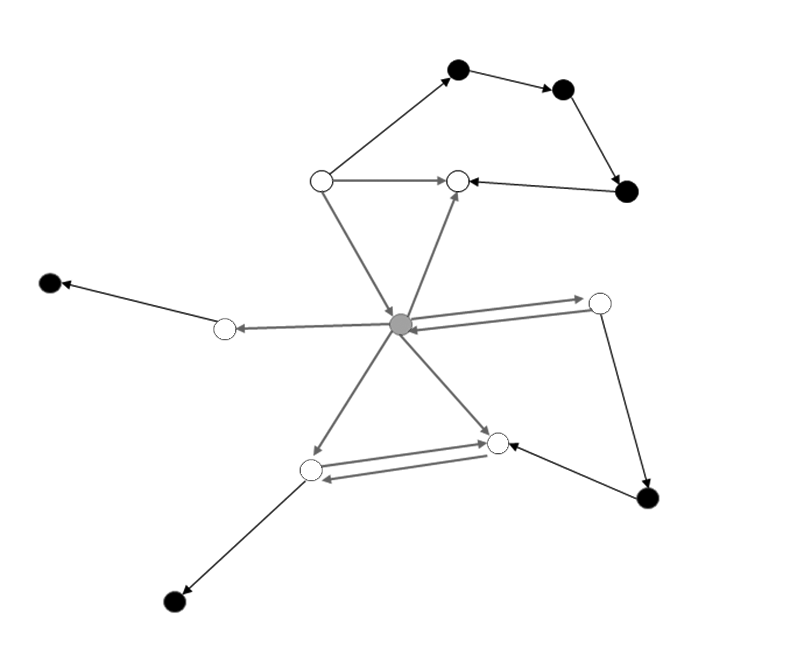
\includegraphics[width=.99\textwidth]{ART_Bielecki/InfoStructcorrectedcopyeditedPP-img001-bw.png}%
 \end{center}%
 \caption{The node-ball of radius 1 centered at a~grey node. The node-ball is a~subgraph composed of the grey node, white nodes, and grey edges.}\label{bie:fig1}
\end{figure}





As it has been mentioned, the information is the structure of the digraph generated by the relation. This structure can be described by the balls. Formally, the node structural information \textit{I}\textit{\textsuperscript{node}} on the set \textit{X}, generated by the relation $\mathcal{R}$ on this set, is the set of all node-balls on the graph \textit{G(X,$\mathcal{R}$)}. Let us consider two nodes that belongs to the same connected component of the graph and all node-balls in the centers in these nodes. If all node-balls of equal radii are isomorphic, meaning they are isomorphic graphs and the isomorphism transforms the center of one ball to the center of another, then the nodes are, by definition, indistinguishable. Otherwise, they are distinguishable. To sum up, the node structural information enables to distinguish the nodes of \textit{G(X,$\mathcal{R}$)}. Indistinguishability of the nodes is an equivalent relation on \textit{V}~(and on \textit{X}, as a~consequence) and equivalent classes generates organization on \textit{X} 
%\label{ref:RND0ZfQQYE0dO}(see Hellerman, 2006).
\parencite[see][]{hellerman_representation_2006}. %
 Consequently, the amount of node information $H^{\textit{node}}$ generates by $\mathcal{R}$~on \textit{n}{}-elementary set \textit{X}~is given as
%$H^{\mathit{node}}=-n\sum _{k=1}^K\frac{n_k} n\log \frac{n_k} n$. (2)
\begingroup
\reqnos
\begin{equation}
H^{\textit{node}}=-n\sum _{k=1}^K\frac{n_k} n\log \frac{n_k} n.
\end{equation}
\endgroup




In formula (2) \textit{K}~denotes the number of equivalent classes and \textit{n}\textit{\textsubscript{k}} denotes the number of elements in the \textit{k}{}-th class. If there are a~few relations on \textit{X}, let us set $\mathcal{R}$\textit{\textsubscript{1}}\textit{,…, $\mathcal{R}$}\textit{\textsubscript{m}}, then all the intersections of the form $Y_{k_1}{\cap}{\dots}{\cap}Y_{k_m}$, where $Y_{k_i}$ denotes the \textit{k}\textit{\textsubscript{i}}\textit{{}-}th equivalence class in the \textit{i}{}-th relation, generate the new partition of \textit{X}~and formula (2) is applied to this new partition. Let us note that supplementing the approach presented in 
%\label{ref:RNDFT6maFg42J}(Bielecki and Schmittel, 2022)
\parencite[][]{bielecki_information_2022} %
 with node existential information is necessary, because otherwise sets with a~different number of elements on which there would be no relation would generate the same amount of information, in both cases equal to zero, which would be counterintuitive.



The node structural information is insufficient because three digraphs that have the same number of nodes: the one without edges, the cyclic one and the complete one would have the same amount of information in each case equal to zero (each two nodes are indistinguishable) that would be a~nonsense result. Therefore, let us introduce edge information. As in the case of node information, we will define edge existential information as information introduced by the fact that a~graph has a~certain number of edges, let us say \textit{m}. Amount of this type of information $H^{\textit{edex}}$ is given as
%\textit{H}\textit{\textsuperscript{edex}} \textit{= log (m+1).} (3)
\begingroup
\reqnos
\begin{equation}
H^{\textit{edex}}=\log (m+1)
\end{equation}
\endgroup

Thus, the node existential information $I^{\textit{edex}}$ is the number of edges in graph $G(X,\mathcal{R})$.

As it was specified above, information is a~structure of the graph generated by a~relation. However, it may happen, for example, that two graphs have the same number of both nodes and edges, and in both cases all nodes are pairwise indistinguishable, but in one graph the edges are indistinguishable, while in the other some edges are distinguishable. Example of such graphs is presented in Fig.2. Therefore, it is necessary to define the edge structural information in similar way as the node structural information was introduced.


\begin{figure}[htbp]
 \centering % Center the figure content

 % First subfigure
 \begin{minipage}[b]{.45\textwidth}
   \centering
   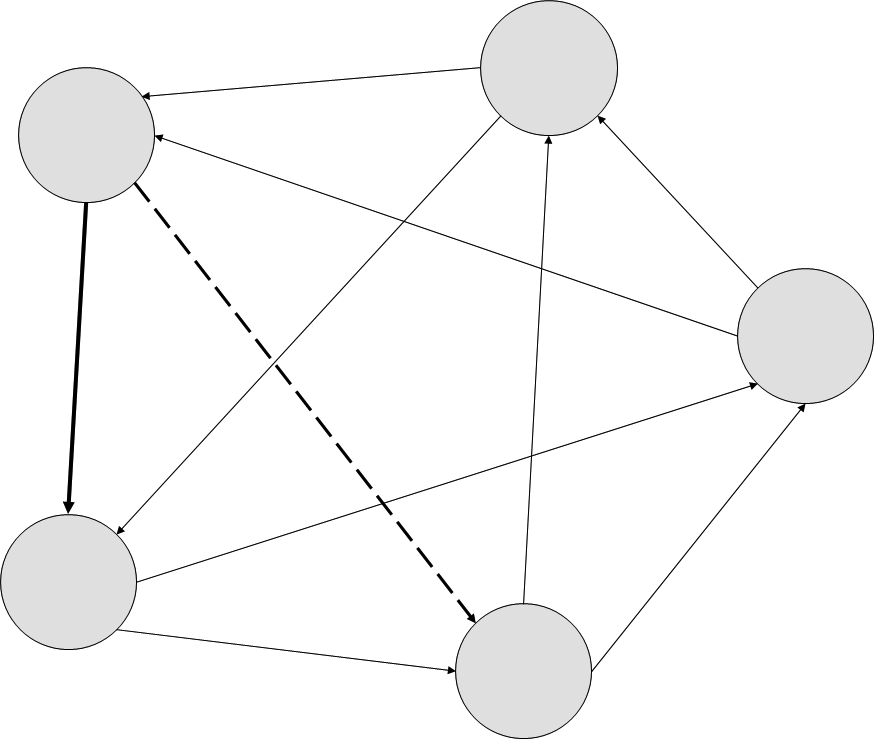
\includegraphics[width=\textwidth]{ART_Bielecki/InfoStructcorrectedcopyeditedPP-img002.png}
   \subcaption{Graph \textit{G}\textsubscript{1}}
 \end{minipage}%
 \hfill
 \begin{minipage}[b]{.45\textwidth}
   \centering
   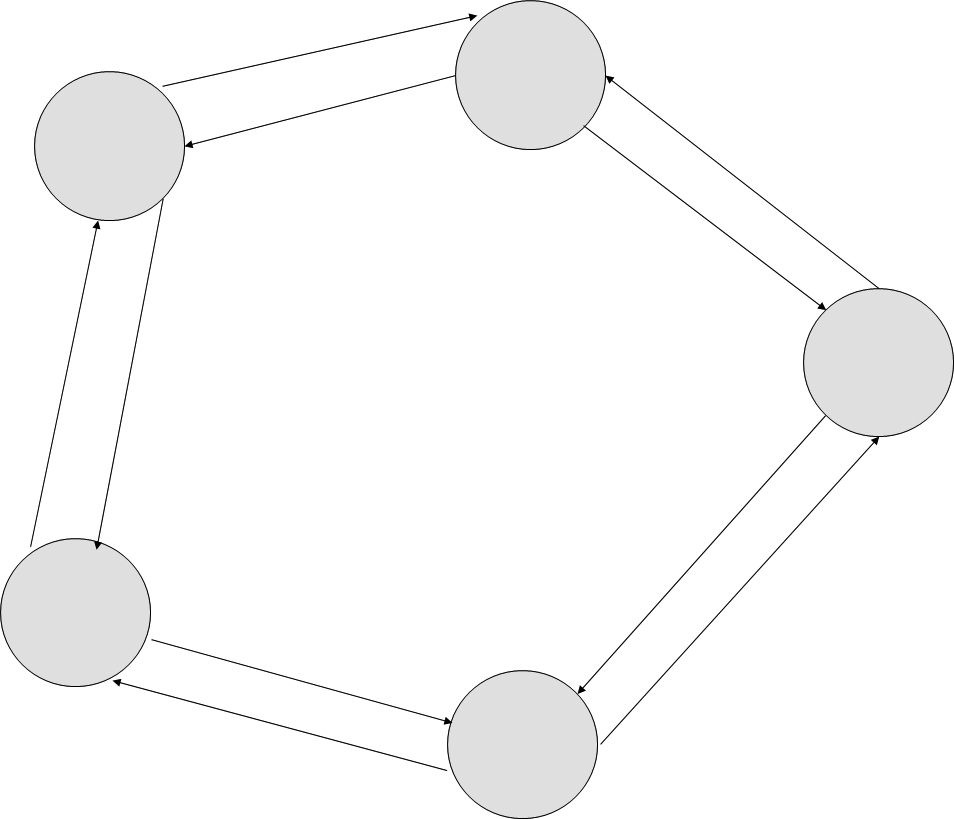
\includegraphics[width=\textwidth]{ART_Bielecki/InfoStructcorrectedcopyeditedPP-img003.png}
   \subcaption{Graph \textit{G}\textsubscript{2}}
 \end{minipage}

 \caption{Two graphs that have the same number of nodes and edges and the same amount of node information and the same amount of both type of existence information but different amount of edge information.}
 \label{bie:fig2}
\end{figure}






So let us define edge-balls on the digraph \textit{G=(V,E)}. An edge ball of radius \textit{1} and a~center in the edge \textit{(u,v)$\epsilon $E} consists of the nodes \textit{u,v,} the edge \textit{(u,v)} and the edge \textit{(v,u)} if it belongs to \textit{E}. The edge-ball of radius \textit{n}~and the center in the edge \textit{e$\epsilon $E} is obtained by completing the edge-ball that has the same center and radius \textit{n-1} by\linebreak all edges adjacent to the nodes of the ball and by completing the nodes that are adjacent to the added nodes. Two edge-balls are, by definition, isomorphic balls if they are isomorphic as the graphs and the isomorphism transforms the center of the one to the center of another. Two edges are indistinguishable if they belong to the same connected component of the graph and all edge-balls of centers in these edges and equal radii are isomorphic edge-balls. Otherwise, the edges are distinguishable. Indistinguishability of edges of a~given graph is an equivalent relation of the set of the graph edges, so it introduces partition of the set of edges. Amount $H^{\textit{edge}}$ of edge information is given as
%$H^{\mathit{edge}}=-m\sum _{t=1}^T\frac{m_k} M\log \frac{m_k} M$, (4)
\begingroup
\reqnos
\begin{equation}
H^{\textit{edge}}=-m\sum _{t=1}^T\frac{m_k} M\log \frac{m_k} M,
\end{equation}
\endgroup
where \textit{m}~denotes the number of edges, \textit{T}~denotes the number of equivalent classes, \textit{m}\textit{\textsubscript{k}} denotes the number of edges in the \textit{k}{}-th class and \textit{M}~is the number of the complete graph that has the same number of nodes. If it is assumed that the relation is antireflexive, then \textit{M=n(n-1)}. Otherwise, \textit{M=n}\textit{\textsuperscript{2}}.  Formally, the node structural information \textit{I}\textit{\textsuperscript{node}} on the set \textit{X}, generated by the relation $\mathcal{R}$ on this set, is the set of all node-balls on the graph \textit{G(X,$\mathcal{R}$)}.



Returning to the example presented in Fig.2 for both graphs we have: \textit{H}\textit{\textsuperscript{ndex}} \textit{= log 6, H}\textit{\textsuperscript{edex}} \textit{= log (11)} and, taken into consideration that in both graphs each two nodes are indistinguishable, \textit{H}\textit{\textsuperscript{node}} \textit{=0.} In graph \textit{G}\textit{\textsubscript{2}} each two edges are indistinguishable, so \textit{H}\textit{\textsuperscript{edge}}\textit{=0.} In graph \textit{G}\textit{\textsubscript{1}} edges denoted by bold arrow and by dashed arrow are distinguishable, because balls of radii 2 are not isomorphic---see Fig.3. For \textit{G}\textit{\textsubscript{1}} on the set of its edges we have the partition (5,5)(20) and, as a~consequence, \textit{H}\textit{\textsuperscript{edge}} \textit{= -10 · 2 · (5/20) log (5/20) = 10.} 


\begin{figure}[htbp]
 \centering % Center the figure content

 % First subfigure
 \begin{minipage}[b]{.45\textwidth}
   \centering
   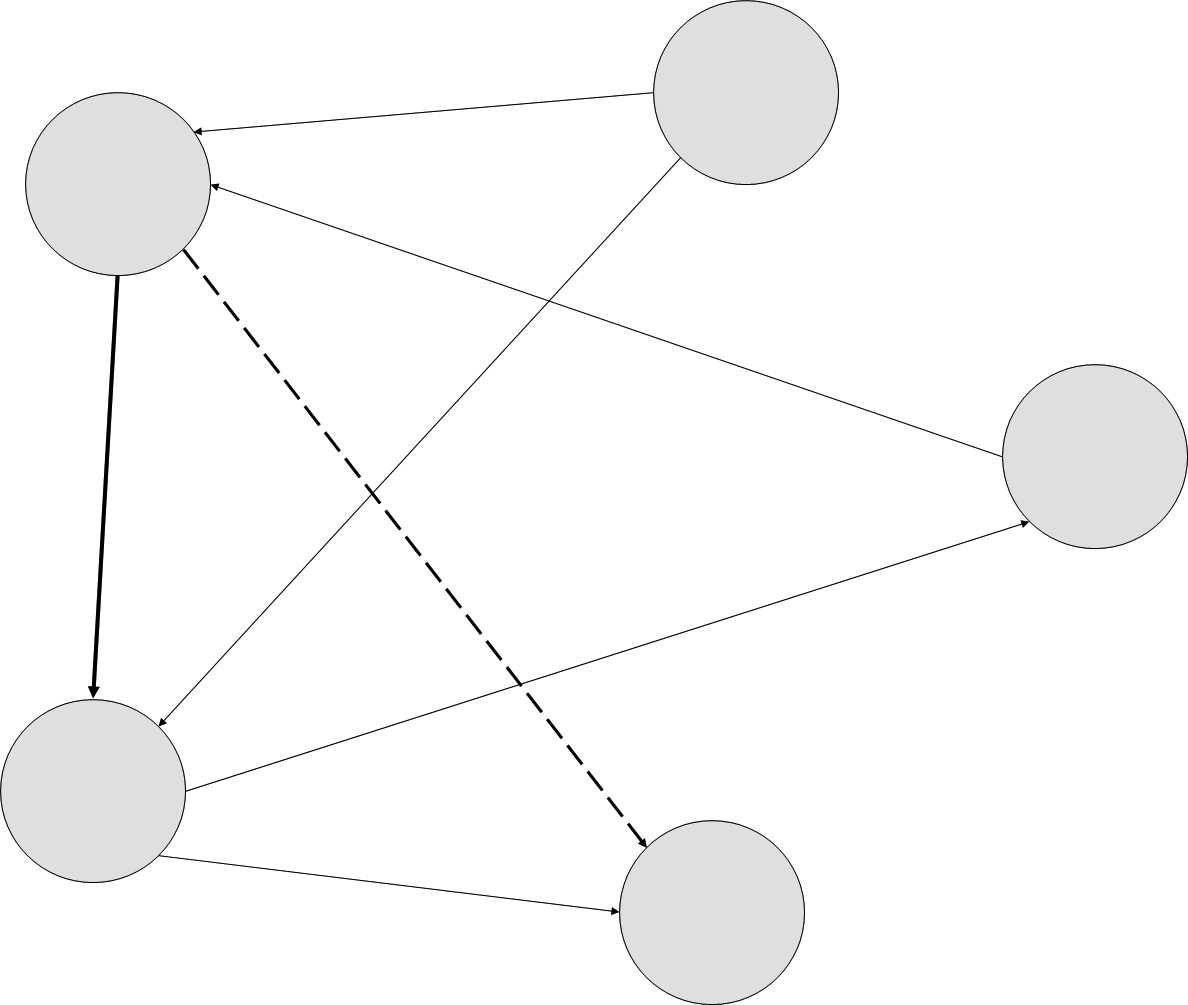
\includegraphics[width=\textwidth]{ART_Bielecki/InfoStructcorrectedcopyeditedPP-img004.png}
   \subcaption{The ball with the center in bold edge and radius \textit{2}}
 \end{minipage}%
 \hfill
 \begin{minipage}[b]{.45\textwidth}
   \centering
   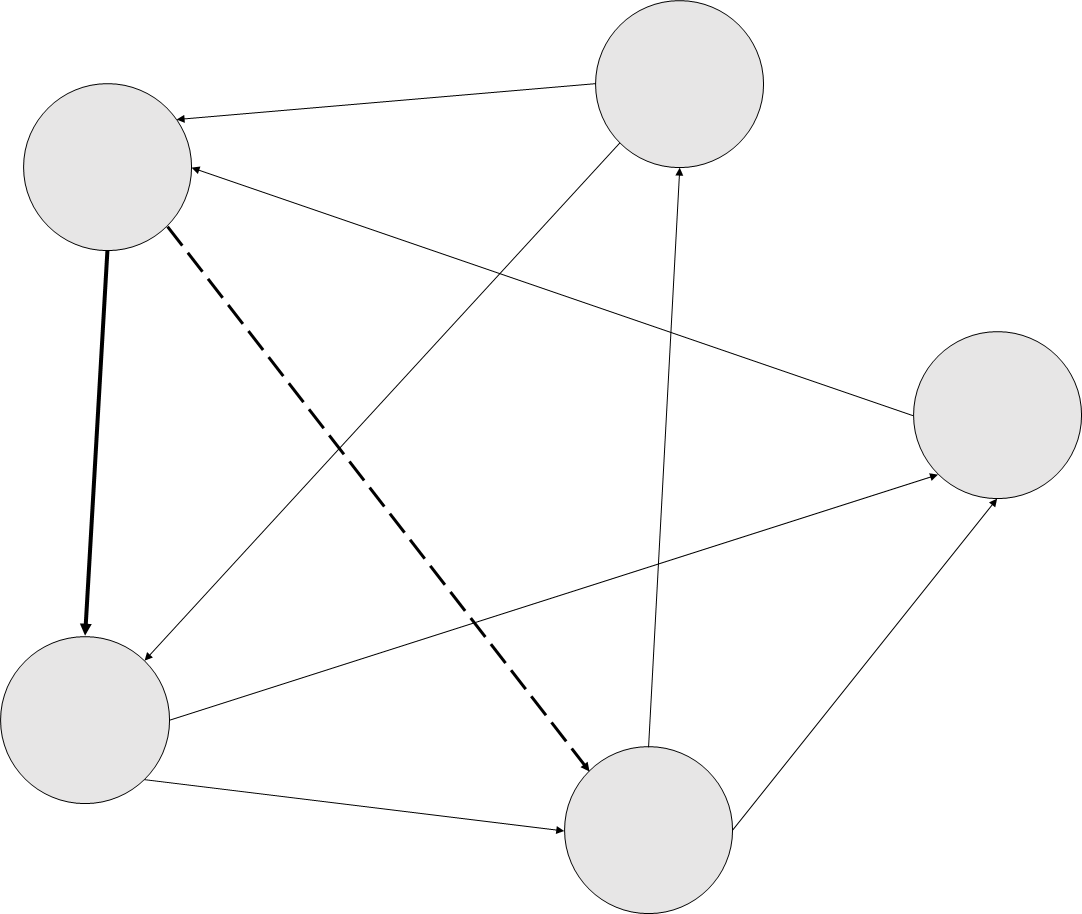
\includegraphics[width=\textwidth]{ART_Bielecki/InfoStructcorrectedcopyeditedPP-img005.png}
   \subcaption{The ball with the center in dashed edge and radius \textit{2}}
 \end{minipage}

 \caption{The balls with centers in bold and dashed edges and radius \textit{2}}
 \label{bie:fig3}
\end{figure}






Let us notice that edges generated by various relations have different labels, so amount of edge information generated by various relations will add up.



Let us summarize the proposed concept. Information is generated on a~given finite set \textit{X} by a~relation defined on this set, which can be easily generalized to a~finite number of relations. This relation, in turn, generates a~structure that is supported by the elements of the set. The generated structure is a~graph whose form is information. This information can be formalized by introducing a~metric into the generated graph, which, in turn, allows to define two types of balls---vertex and edge ones. Said balls define different types of structural information introduced by the said relation. Let us discuss the introduced sorts of information.



\textbf{Node existential information} is given by the number of elements of the set X, on which the information is generated by a~relation or relations on it. This sort of information determines upper boundary of the amount of structural information that can be generated on \textit{X}.



\textbf{Edge existential information} is given by the number of edges in the graph generated by a~given relation on \textit{X}. This sort of information determines what part of the possibility of generating information on \textit{X} was utilized by a~given relation.



\textbf{Node structural information} determines which elements of the set are related to each other and how the introduced relation differentiates the elements of the set in the context of the overall structure, i.e. the graph generated by this relation.



\textbf{Edge structural information} determines the character of a~given relationship between two specific elements in the context of the whole information generated by the introduced relation on~\textit{X}.


Thus, the information introduced by a~relation on a~base set is constituted by existential information, which consists of node existential information and edge existential information, and structural information, that consists of node structural information and edge structural information.



\section{Some remarks about the proposed concept of information}

Let us discuss some aspects and nuances of the proposed concept of information. Research on structured information is conducted in a~broad field in philosophy. Mathematical tools are often used for this purpose 
%\label{ref:RNDPSilXHGCt6}(Schroeder, 2019a).
\parencite[][]{schroeder_analogy_2019}. %
 At the most general level, the concepts of structural information, usually in mathematically oriented studies, are related to the concept of distinguishability-indistinguishability of elements of a~given set 
%\label{ref:RNDplOa9phPxk}(Schroeder, 2019b),
\parencite[][]{dodig-crnkovic_theoretical_2019}, %
 which is sometimes connected with operational aspect of information 
%\label{ref:RND6LXziU0nQw}(Bateson, 1951).
\parencite[][]{bateson_information_1951}. %
 In physical and biological aspects, structural information is considered as a~physical property represented by the spatial and temporal configuration of matter and follows the laws of physics 
%\label{ref:RND1XkdHoLrOs}(Ebeling and Feistel, 2015; Davies, 2019).
\parencites[][]{ebeling_selforganization_2015}[][]{davies_demon_2019}. %
 The effect of the large number of research directions on structured information is, among other things, the fact that the term \textit{structural information} is used with different meanings, depending on the research context. In this paper the term \textit{structure} has only mathematical meaning and concerns the form of the generated graph \textit{G(X,R)} and, in particular, it should not be confused with the meaning used in physics, cosmology and in some contexts of philosophy 
%\label{ref:RNDx2Tl0sKcJY}(see, e.g., Burgin, 2011).
\parencite[see, e.g.,][]{burgin_information_2011}. %
 The presented concept of information seems to be pioneering. Therefore, it is hard to point out papers in which the key terms are used in similar meaning. Nevertheless, the idea of structural information is rooted in the Hellerman's concept of \textit{organization}  
%\label{ref:RNDWClJfv6ZqZ}(see Hellerman, 2006; 2016).
\parencites[see][]{hellerman_representation_2006}[][]{hellerman_animate_2016}.%




The possibility of generalizing the presented concept is an important problem in the philosophical and mathematical aspect. At the present stage, the proposed concept has been developed for finite sets and binary relations. For finite sets and non-binary relations, it is enough to use hypergraphs 
%\label{ref:RNDHAmZRzyGll}(Berge, 1989)
\parencite[][]{berge_hypergraphs_1989} %
 instead of classical graphs. Generalization to the case of infinite sets is a~much more serious problem. First, it should be emphasized that the concept in its present form was developed for specific biological and biochemical applications 
%\label{ref:RNDmcqM5VyStx}(Bielecki, 2015; Bielecki and Schmittel, 2022),
\parencites[][]{bielecki_general_2015}[][]{bielecki_information_2022}, %
 where infinite sets do not occur. Furthermore, it demonstrates utility in cognitive maps problems, where infinite sets do not occur neither. Therefore, its application possibilities and formalization were more important than purely philosophical aspects. Returning to the problem of generalization to the case of infinite sets, instead of the number of vertices in the graph, a~certain measure should be used, which is undoubtedly feasible. However, a~significant difficulty will be replacing the graph with some other mathematical structure that will generate appropriate equivalence classes. At the present stage, it is impossible to determine whether this is doable.



It should be stressed that the structural information cannot be reduced to quantitative aspect. The presented approach does not introduce such reductionism. The form of the generated graph represents the qualitative aspect of structural information, whereas the way of calculating its amount is its quantifying aspect.



Information, in general, has both ontological and epistemological dimensions. Referring to the ontological aspect, the situation is analogue as with energy that, from the most general point of view, can be kinetic or potential, which has far-reaching consequences for its agency. It seems, that in the context of diversity of information, reality is much richer than in the context of various forms of energy. In addition to the four types information defined in the paper---two structural and two existential---there exists at least information generated by possible node labelling---see also remarks at the end of Section 4. Additionally, information generated by the fact that the generating relation is the used one is the another type of information but, in this case, is not structural. Referring to the epistemological aspect, node and edge information point at the various aspects of the form of the generated graph, the form of which is information generated by the relation defined on the base set.



\section{Application to cognitive maps}

As it was mentioned in the first section, the presented concept of information was dedicated to studies that concern life processes. It can be, however, successfully utilized to cognitive maps. This application is initially discussed in this section. Thus, the research that was used to create the analyzed cognitive maps, is described in subsection 3.1. In the subsequent subsection application of the proposed concept to analysis of cognitive maps is described.



\subsection{Cognitive maps in psychology, management and philosophy}



The problem of legitimate methods of knowing the world and the adequate representation of knowledge about the world is a~classic issue of epistemology. Until the end of the 19\textsuperscript{th} century, it was considered only in the context of human cognitive abilities. In the 20\textsuperscript{th} and 21\textsuperscript{st} centuries, these issues included research on the perception of the world by animals and the representation of the world in the context of autonomous robots 
%\label{ref:RNDG69MgxrnAg}(see, e.g., Bielecki, 2021).
\parencite[see, e.g.,][]{bielecki_systemic_2021}. %
 In this context representation by using cognitive maps and various logical representations are studied. The discussion of this stream of scientific investigation in philosophical aspect is presented in 
%\label{ref:RNDlwWJW0gMhX}(Rescorla, 2009).
\parencite[][]{rescorla_cognitive_2009}.%




Authors of \textit{Visible thinking} 
%\label{ref:RND42SCGRhBeT}(Brysson et al., 2004)
\parencite[][]{brysson_visible_2004} %
 start their book with the statement that \textit{thinking really matters.} So having an explicit picture of the thinking process and the concepts would be a~revolutionary step to revealing, analysing and improving the thinking process. Cognitive maps are the first candidate for such endeavour. Although the first cognitive maps were attributed to William James, their first confirmed use was done by in 1948 
%\label{ref:RNDuDLcDjMaBc}(Tolman, 1948).
\parencite[][]{tolman_cognitive_1948}. %
 At that time these were cognitive space representations located in hippocampus. Conceptual maps as we view them now only start with George Kelly in 1955. He compared human beings to scientists who are continuously making hypothesis, formulating theories and checking them empirically. According to Kelly, we are continually carrying out experiments to explain our surrounding reality. We do this to better navigate our life. Kelly's idea had a~huge influence on researchers concerning cognitive processes. Whole trend to study naive theories became a~tool of studying conceptual changes concerning children and youth has arisen, what had serious consequences for education 
%\label{ref:RNDUAx0VOcT7K}(Kuhn, 1989; Vosniadou, 1996).
\parencites[][]{kuhn_children_1989}[][]{vosniadou_towards_1996}.%




Unfortunately, those researches have either general character 
%\label{ref:RNDtmxvlI0snn}(e.g., Kruglansky, 1980)
\parencite[e.g.,][]{kruglansky_lay_1980} %
 or concern theories of indigenous domain having basis meaning for human's life (mainly physic concepts, natural concepts, theories of mind, etc.), or connected with teaching individual subjects at school.



Testing causal maps as cognitive constructs was applied also in developmental psychology---its action was conditioned there with help of mathematic tool---Bayes' network. It was a~trial to understand process of creating causal connections 
%\label{ref:RNDpuzxJMIHup}(Gopnik et al., 2004).
\parencite[][]{gopnik_theory_2004}. %
 Psychologists do not only want to know rules of passing on the knowledge, as it is in the theory of social learning 
%\label{ref:RND45JodZszxo}(Bandura, 1977),
\parencite[][]{bandura_social_1977}, %
 but also they want to understand the mechanism of gaining new knowledge indirectly derived from world's observation. Of course children do not know anything about any maps. Those maps have hidden character; they are only a~construct, which is seen and later on conditioned by scientists. Modelling like that allows on computer simulation and generating analogous ``behavior'' of system with applications, among others, in robotics 
%\label{ref:RNDj5ISJZtsP2}(Chaib-draa, 2002).
\parencite[][]{chaib-draa_causal_2002}.%




Research like this is carried on yet in children from the age of 30 months. For example, specific arrangement of simple objects on the stand with a~detector evokes sound signal and researchers observe how children come up to an idea of when this sound is occurring 
%\label{ref:RND9oSCjgeDrV}(Gopnik et al., 2001).
\parencite[][]{gopnik_causal_2001}. %
 Those researches are very general so that they are useful in organizational diagnosis only in limited scope. Gopnik is ruthless opponent of directly asking tested person about causal connections. As she wrote 
%\label{ref:RNDk1Pb0M2Kkt}(Gopnik et al., 2004),
\parencite[][]{gopnik_theory_2004}, %
 she is almost sure that adults would have made a~mistake if they were directly asked to give causal connections, even if they would do well in tasks requiring this connections. It means that people are not able to directly judge their cognitive constructs. It is worth taking note of the fact that accepting constructivist assumptions concerning how the mind works does not mean that they are also supporters of the second from proposed approaches---domain specificity, meaning belief that it is hard to talk about general rules of building cause-result connections in isolation from content. Although some researchers see the relationship between the map and the real world. For instance Leslie states that ``the infant is a~specialized processor of information with an architecture that (in part) reflects properties of the world'' 
%\label{ref:RNDFExlCYAshV}(Leslie, 1994)
\parencite[][]{hirschfeld_tomm_1994}%
. Such ontological references are infrequent. Usually cognitive maps are simply treated as educational or management tools in multiple such as education 
%\label{ref:RNDYmTxe1blie}(Moon et al., 2011; Barton et al., 2016),
\parencites[][]{moon_applied_2011}[][]{barton_mind_2016}, %
 management 
%\label{ref:RNDewomO7kPDu}(Brysson et al., 2004; Lengyel and Sarah, 2023),
\parencites[][]{brysson_visible_2004}[][]{lengyel_capturing_2023}, %
 economy 
%\label{ref:RNDCQpjIgCSxY}(Voss et al., 1986)
\parencite[][]{voss_informal_1986} %
 and on leadership 
%\label{ref:RND9Lgeivrj6b}(Offermann, Kennedy and Wirtz, 1994).
\parencite[][]{offermann_implicit_1994}. %
 In cognitive social psychology there is whole tradition of researches concerning general understanding of the world, systems thinking, organizational diagnosis 
%\label{ref:RNDZP4i5eyr3l}(Bielecki and Nieszporska, 2019; Bielecki and Stocki, 2010; Laukkanen, 1998).
\parencites[][]{bielecki_analysis_2019}[][]{bielecki_systems_2010}[][]{eden_conducting_1998}.%




A~great step in the use of cognitive maps was done after introduction of a~popular software for generating and sharing cognitive maps 
%\label{ref:RNDR4xF0PQd5r}(Novak and Cañas, 2006).
\parencite[][]{novak_origins_2006}. %
 As a~result today there are servers all around the world which host results of research and educational tools based on Cmaps.\footnote{See https://cmap.ihmc.us/cmapserver/ } In real analysis of concepts with the use of cognitive maps we encounter the problem of complexity of such maps. For instance in the study of positive concepts of mental health 
%\label{ref:RNDxRIQxZkqMX}(Iasiello et al., 2023)
\parencite[][]{iasiello_whats_2023} %
 after review of all the relevant literature arrived at 155 measures and 410 original constituent dimensions. These were reduced to a~set of 21 themes. Figure 4 shows an example of an expert map of an effective cooperative.



\begin{figure}
 \begin{center}
 \begin{adjustwidth}{-.1\textwidth}{}
 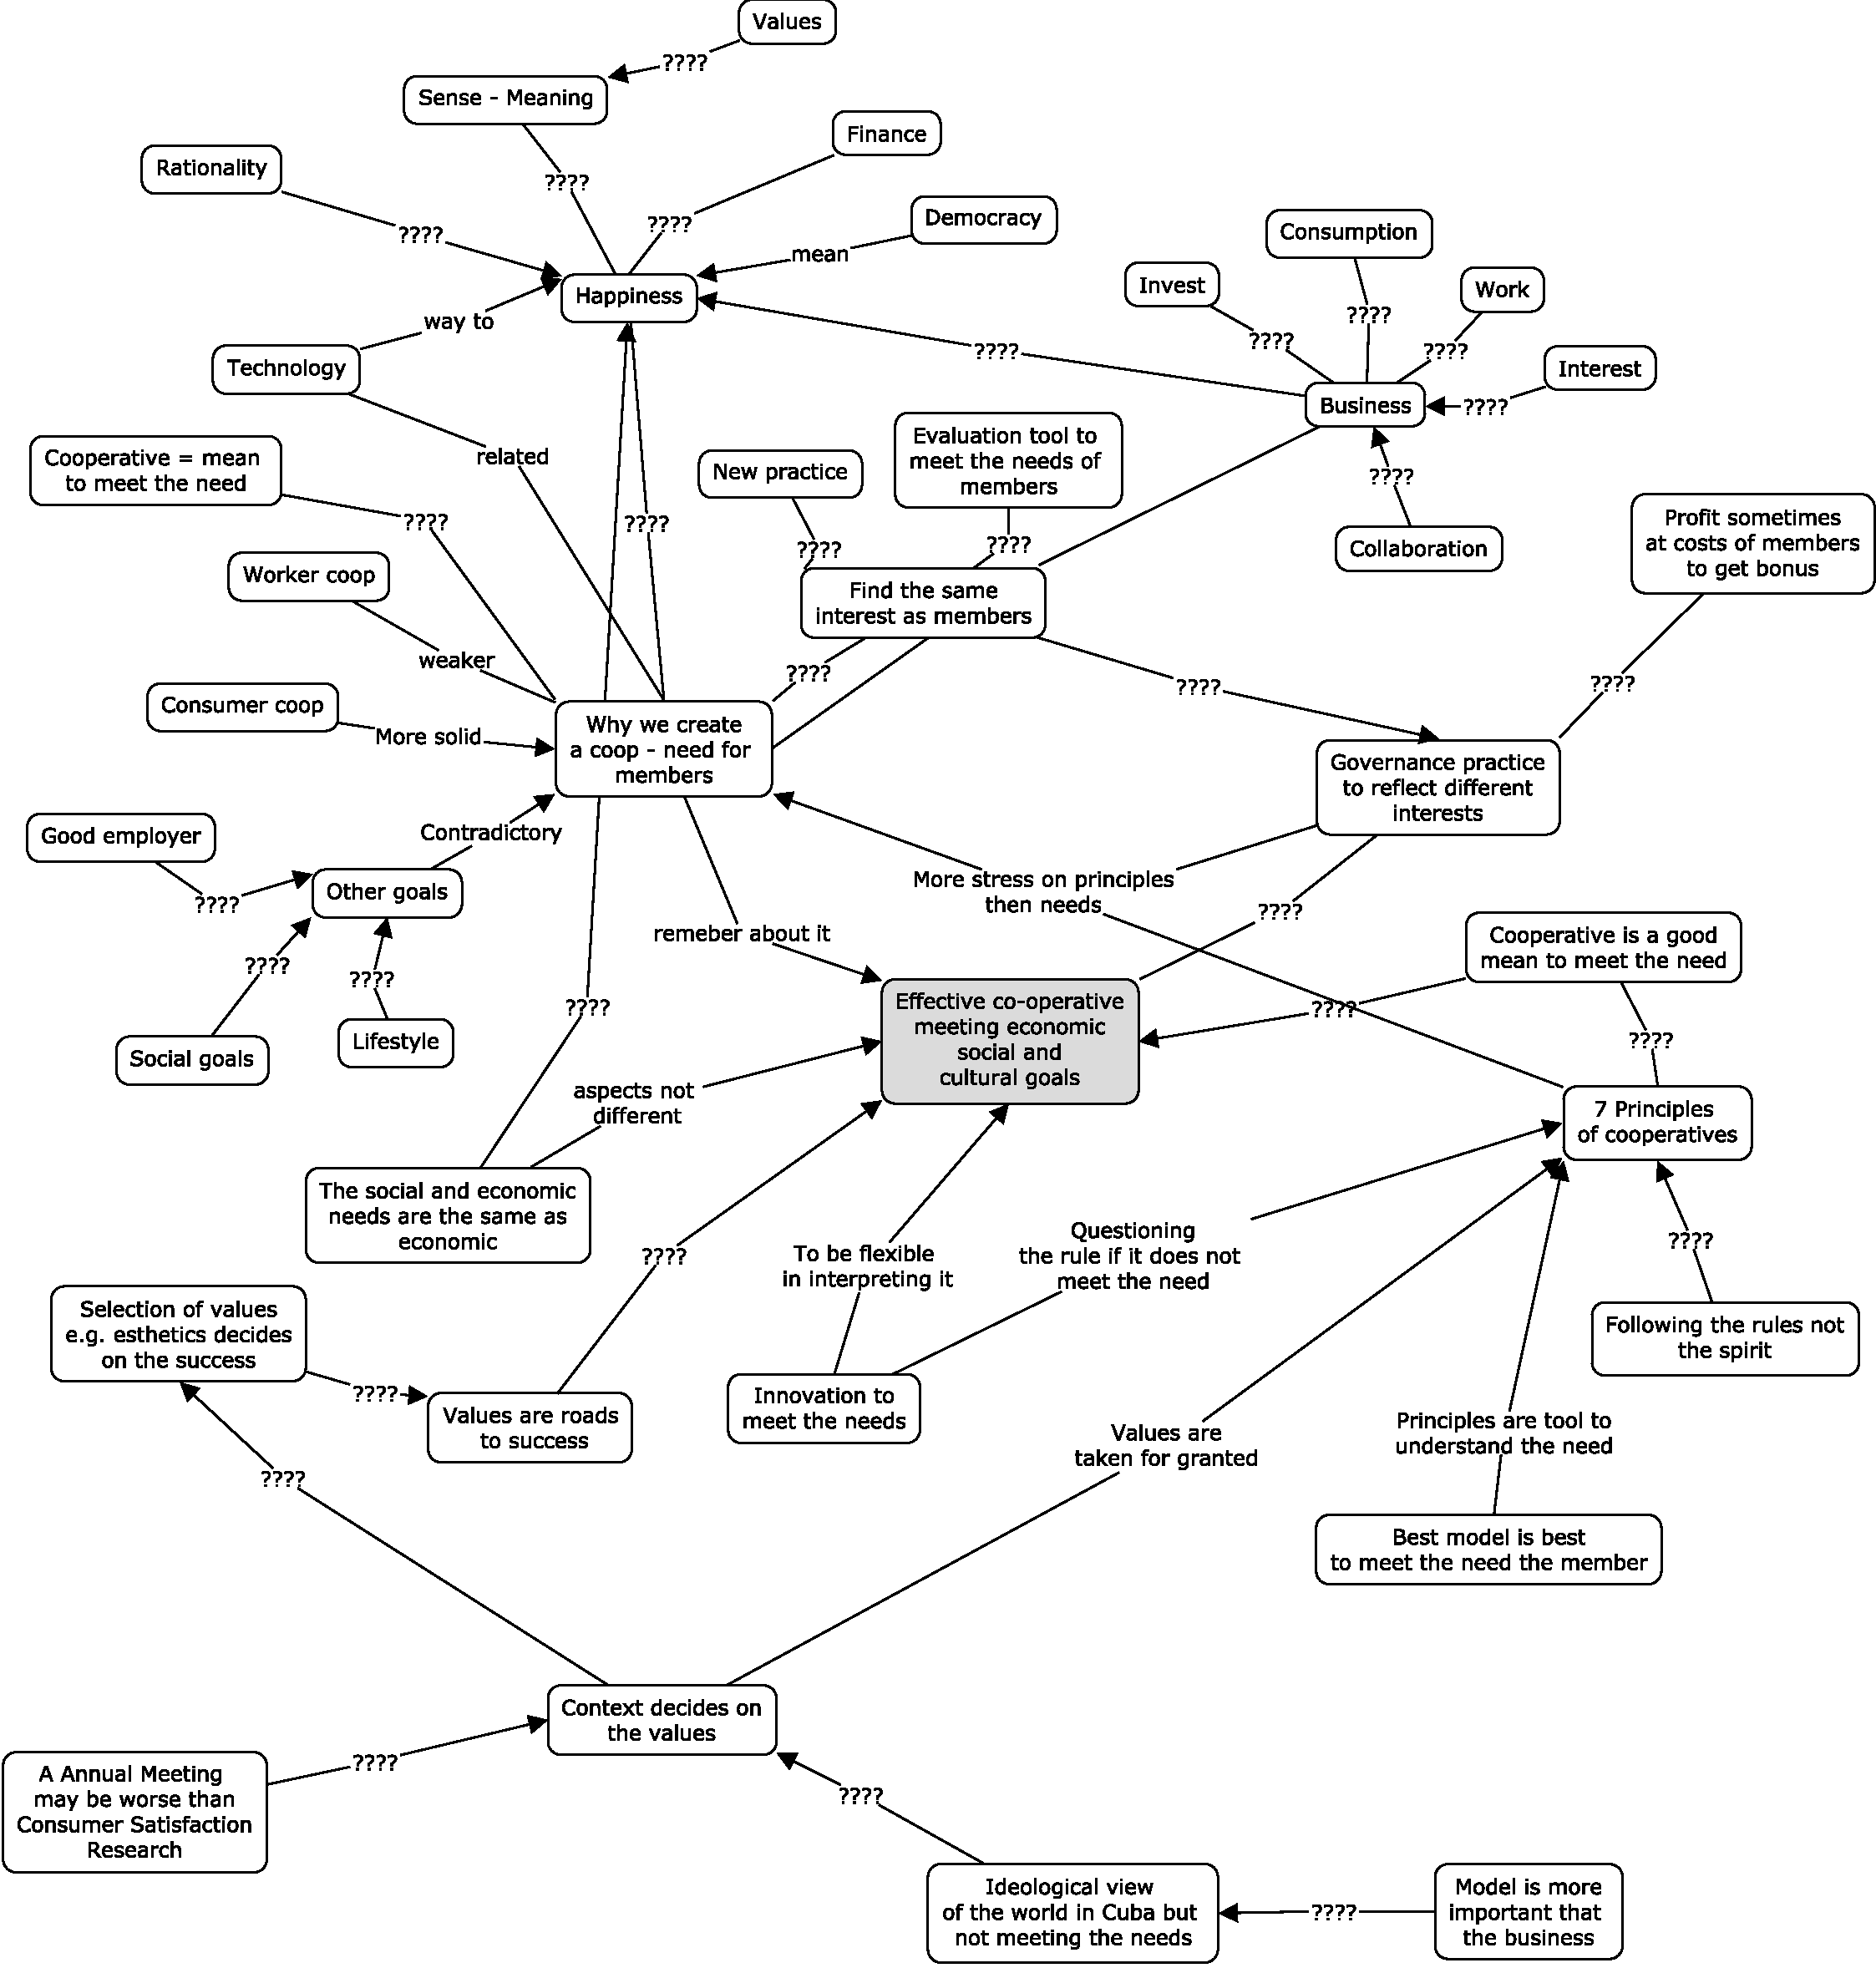
\includegraphics[width=1.2\textwidth]{ART_Bielecki/fig6.pdf}%
 \end{adjustwidth}
 \end{center}%
 \caption{An expert map of an effective coopertive 
 %\label{ref:RNDRQ89DmmkM0}(Stocki, submitted).
 \parencite[][]{stocki_tacit_nodate}.}\label{bie:fig4}
\end{figure}




The concept of structural information, and particularly its analytic opportunities related to balls of different diameter might allow focus on such a~huge 410 
%\label{ref:RNDn7F9scOnGs}(Iasiello et al., 2023)
\parencite[][]{iasiello_whats_2023} %
 or 40 elements map in Fig.4 without the necessity to synthesize it.



\subsection{Application the concept of structural information to cognitive maps}



How people think in the economic context, and particularly in management has a~direct impact on companies' success. No wonder, management is one of the domains that uses the tool such as map analysis most often. Preliminary results indicate that managers' cognitive maps, may impact the decision making process and, as a~result, success of a~company. Thus, investigation of the structure and complexity of such maps can be in such sort of studies in psychology of management. The example of cognitive maps obtained during these studies is presented in Fig.5. The managers were asked of drawing cognitive maps on which the notion \textit{responsibility} was the starting point. On the cognitive map it was necessary to place all the concepts that the concept of \textit{responsibility} affects or which have an impact on \textit{responsibility}. It was also necessary to take into account the mutual influence of the placed concepts.



The presented concept of information, at its current, initial stage, is not a~powerful enough tool to study the structure of natural language utterances, much less the meaning of utterances. Nevertheless, it is sufficient to study the structure of cognitive maps without analyzing their lexical content. Let us consider two cognitive maps obtained during the investigations described in subsection 4.1 presented in Fig.5. The arrows on the cognitive maps means that \textit{notion A~affects notion B.} This is a~relation in the sense of the concept of structural information. The graphs generated by the said relation generates the graphs shown in Fig.6. The filled nodes correspond to the utterance \textit{responsibility}, that was the starting point of the studies.

\begin{figure}[htbp]
\begin{adjustwidth}{-.1\textwidth}{}
  \begin{minipage}{.5\linewidth}
    \centering
  \begin{tikzpicture}[scale=0.6, transform shape,
   centernode/.style={ellipse, align=center, minimum width=2cm},
        mynode/.style={draw, align=center, rounded corners, minimum width=1cm, minimum height=0.5cm},
        myarrow/.style={<-, >=latex, thick},
        node distance=1cm and 2cm
    ]
    
    \node[centernode] (responsibility) {Responsibility};
    \node[mynode, above left=of responsibility, xshift=1.5cm] (submission) {Submission to\\ supervisors};
    \node[mynode, above right=of responsibility, xshift=-1cm] (decision) {Decision\\ making};
    \node[mynode, below right=of responsibility,yshift=.5cm, xshift=-.7cm] (action) {Action};
    \node[mynode, below left=of responsibility, yshift=1cm, xshift=.5cm] (leading) {Leading a team\\ of people};
    \node[mynode, below=of responsibility] (response) {Response to\\ problems};
    
    \draw[myarrow] (submission) -- (responsibility);
    \draw[myarrow] (decision) -- (responsibility);
    \draw[myarrow] (action) -- (responsibility);
    \draw[myarrow] (leading) -- (responsibility);
    \draw[myarrow] (response) -- (responsibility);
  \end{tikzpicture}
	\end{minipage}%
	 \begin{minipage}{.6\linewidth}
  \centering
  \begin{tikzpicture}[scale=0.6, transform shape,
   centernode/.style={ellipse, align=center, minimum width=2cm},
                  mynode/.style={draw, align=center, rounded corners, minimum width=1cm, minimum height=0.5cm},
             myarrow/.style={->, >=latex, thick},
             dbarrow/.style={<->, >=latex, thick},
             node distance=1cm and 2cm
         ]
         
         % Central node
         \node[centernode] (responsibility) {Responsibility};
         
         % Top nodes
         \node[mynode, above left=of responsibility, yshift=1cm, xshift=1cm] (loyalty) {Loyalty};
         \node[mynode, above=of responsibility, xshift=1cm] (honesty) {Honesty};
         \node[mynode, above=of honesty, xshift=1.5cm] (tolerance) {Tolerance};
         
         % Bottom nodes
         \node[mynode, below left=of responsibility,  xshift=1.5cm] (respEmployees) {Responsibility for\\ other employees};
         \node[mynode, below right=of responsibility, xshift=-.5cm] (professionalism) {Professionalism};
         
         % Draw arrows
         \draw[myarrow] (loyalty) -- (responsibility);
         \draw[myarrow] (honesty) -- (responsibility);
         \draw[dbarrow] (tolerance) -- (honesty);
         \draw[myarrow] (responsibility) -- (professionalism);
         \draw[dbarrow] (respEmployees) -- (responsibility);
         \draw[dbarrow] (respEmployees) -- (professionalism);
         \draw[dbarrow] (honesty) -- (professionalism);
         \draw[dbarrow] (tolerance) -- (professionalism);
  \end{tikzpicture}
\end{minipage}
\end{adjustwidth}
 \caption{Examples of two cognitive maps obtained during investigations described in subsection 4.1.}
 \label{fig:maps}
\end{figure}
\begin{figure}[htbp]
 \centering % Center the figure content

 % First subfigure
 \begin{minipage}[b]{.4\textwidth}
   \centering
   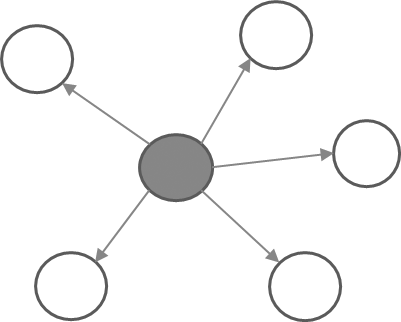
\includegraphics[width=\textwidth]{ART_Bielecki/fig9.png}
   \subcaption{Graph \textit{G}\textit{\textsubscript{1}}}
 \end{minipage}%
 \hfill
 \begin{minipage}[b]{.53\textwidth}
   \centering
   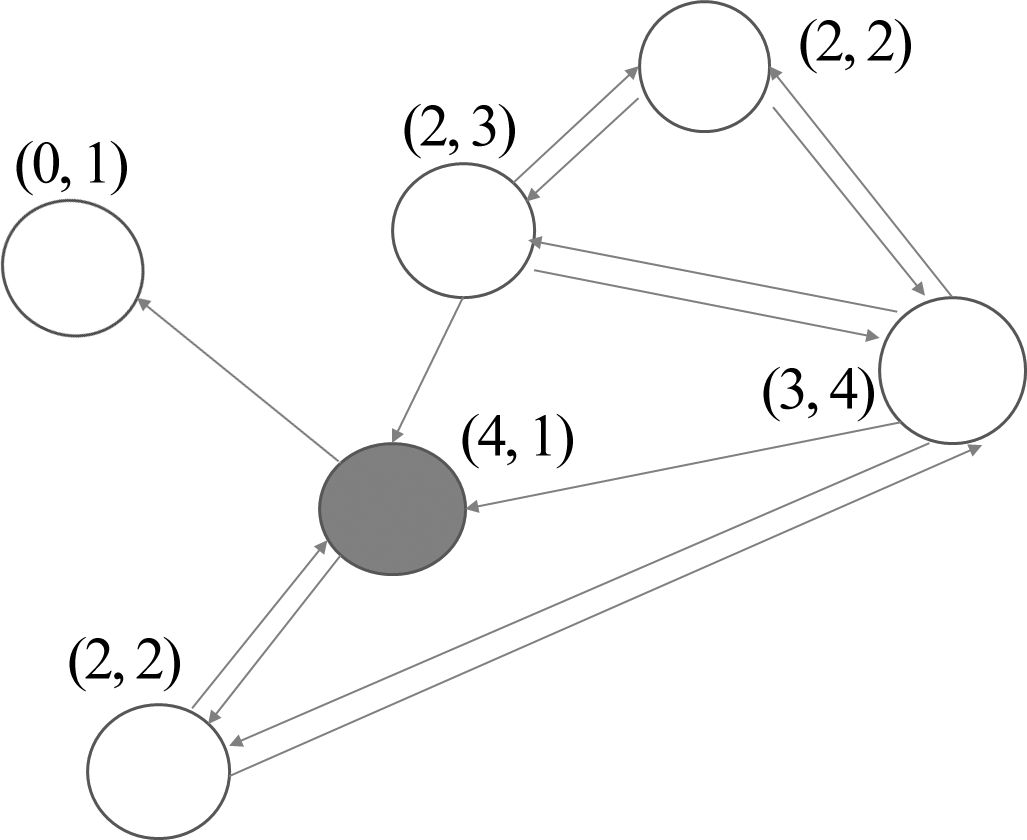
\includegraphics[width=\textwidth]{ART_Bielecki/fig10.png}
   \subcaption{Graph \textit{G}\textit{\textsubscript{2}}}
 \end{minipage}
 \caption{The structure of cognitive maps presented in Fig.5. The numbers in parentheses in graph G\textsubscript{2} denote indegree and outdegree of the node.}
 \label{bie:fig6}
\end{figure}




Let us consider graph \textit{G}\textit{\textsubscript{1}} presented in Fig.6(a). It consists of six nodes and five edges, thus---see formulae (1) and (3) we have
\[
H^{\textit{ndex}} = \log 7 \approx 2.8,
\]
\[
H^{\textit{edex}} = \log 6 \approx 2.6.
\]

The filled node is distinguishable from any other whereas the others are pairwise indistinguishable. Thus, on the set of the nodes we have partition \textit{(5,1)} (in the Hellerman sense) and, as a~consequence
\[
H^{\textit{node}} = -6 \left[ \left(\frac{5}{6}\right) \log\left(\frac{5}{6}\right) + \left(\frac{1}{6}\right) \log\left(\frac{1}{6}\right) \right] \approx 3.9.
\]

It is obvious that all edges are pairwise indistinguishable, so
\[
H^{\textit{edge}} = 0.
\]

Graph \textit{G}\textit{\textsubscript{2}} consists of six nodes and thirteen edges, so
\[
H^{\textit{ndex}} = \log 7 \approx 2.8,
\]
\[
H^{\textit{edex}} = \log 13 \approx 3.7.
\]

In graph \textit{G}\textit{\textsubscript{2}} each two nodes are distinguishable. Indeed, apart from two nodes, all others have pairwise different bi-labels that encoded indegree and outdegree of the node---see Fig.6(b). Thus, they are pairwise distinguishable. Two nodes that have bi-label \textit{(2,2)} are also distinguishable because the node-balls of radius \textit{1} and centers at these points are not isomorphic. The one of two node-balls is a~subgraph that consists of the nodes labeled as \textit{(2,2), (3,4), (2,3)} and six edges connecting them. The second one consists of the nodes labeled as \textit{(2,2), (3,4), (3,2)} and five edges connecting them. Since the numbers of edges in two these balls are different, the node-balls are not isomorphic. As a~consequence, the partition in the Hellerman sense of the set of nodes is \textit{(1,1,1,1,1,1)} and
\[
H^{\text{node}} = -6 \left[ 6 \left(\frac{1}{6}\right) \log\left(\frac{1}{6}\right) \right] \approx 15.5.
\]

In graph \textit{G}\textit{\textsubscript{2}} each pair of edges are distinguishable because for any two edges it is not true that bi-labels of the nodes from which the edges originate are equal and it is not true that bi-labels of the nodes to which the edges enters are equal. Furthermore, let us notice that in the context of the considered cognitive maps self-reference of the relation has no sense, so it is natural to assume that \textit{M=n(n-1)=6·5=30.} So, we have a~partition in the sense defined in 
%\label{ref:RNDYnS0vMCERo}(Bielecki and Schmittel, 2022)
\parencite[][]{bielecki_information_2022} %
 equal to \textit{(1,1,1,1,1,1,1,1,1,1,1,1,1)(30)} and, as a~consequence,
\[
H^{\text{edge}} = -13 \left[ 13 \left(\frac{1}{30}\right) \log\left(\frac{1}{30}\right) \right] \approx 27.7.
\]

Thus, graphs \textit{G}\textit{\textsubscript{1}} and \textit{G}\textit{\textsubscript{2}} have the same amount of node existential information. Graph \textit{G}\textit{\textsubscript{2}} has, however, significantly more amount of edge existential information---\textit{3.7} bites versus \textit{2.6} bites. Furthermore, amount of structural information is far more greater in graph \textit{G}\textit{\textsubscript{2}}---\textit{15.5} versus \textit{3.9} bites in the case of node structural information and \textit{27.7} versus \textit{0} bites in the case of edge structural information.



As it has been mentioned, at the current stage of studies it is impossible to conduct deep lexical analysis in the frame of the proposed concept. Nevertheless, labeling could be introduced to distinguish the central term in the analyzed maps---\textit{responsibility---}from the other terms. In the case of two analyzed maps, however, such labeling does not provide any additional information. In fact, in the case of graph \textit{G}\textit{\textsubscript{1}} it would distinguish the central notion from the other ones, but it is already distinguished with the partition of the set of the nodes introduced by the considered relation. In the case of graph \textit{G}\textit{\textsubscript{2}} all nodes are distinguishable by the considered relation.



It should be stressed that in the context of structural information, labeling is not arbitrary, but encodes information about the nature of the elements of the base set. Labeling by the common label the atoms of the same chemical elements is a~typical example 
%\label{ref:RNDizAbmzmYKf}(see Bielecki and Schmittel, 2022).
\parencite[see][]{bielecki_information_2022}. %
 In this paper, in the analyzed cognitive maps, the term \textit{responsibility} is highlighted as the base term provided by the researcher to which referred all other terms used by the person being examined. Therefore, without falling into the trap of lexical meaning, it was proposed to label this word with a~unique label as a~concept having a~unique status in the study. The remaining vertices were labeled with a~different label, but all with the same one. This labeling was done in order to distinguish the base term without going into lexical analysis.



\section{Concluding remarks}

Let us summarize the proposed concept of information and the presented example of its application. The concept of information at the current stage of the studies is formulated in purely mathematical way. The definitions of various types of information have been put forward and their basic properties have been specified. This was done with care for formal correctness and completeness. Although the concept was originally dedicated to applications for analysis of biological structures and processes 
%\label{ref:RNDIJr53JnJPy}(see Bielecki, 2015)
\parencite[see][]{bielecki_general_2015} %
 and was preliminary tested by using to analysis of molecular cybernetics 
%\label{ref:RNDBmHEi1m1dC}(see Bielecki and Schmittel, 2022)
\parencite[see][]{bielecki_information_2022} %
 it turned out that the concept is also applicable to analysis of cognitive maps. As for the analyzed example of applications, formal analysis of such maps with the assistance of structural information concept allows the researchers to go beyond from the simple analysis of the map content to the analysis of the maps structure and complexity. As is visible in the example above, we can, for instance, analyze the role of the central concept of responsibility in detail showing that in the first map if removed, it disintegrates the structure of the whole graph, whereas the same removing of the central concept from the second graph causes only partial disintegration of the structure of the graph. This means that in critical moments in the decision making process, when some important aspect is undermined, the first manager may have no indication how to behave whereas the second one may reconstruct the decision with the help of a~substitute. Such formal analysis of the concepts make visible properties of our thinking that were, so far, treated as tacit. Furthermore, the proposed approach allow the researcher to calculate precisely amount of information in the cognitive maps.



\end{artengenv2auth}


%\begin{artengenv}{Wojciech P. Grygiel}
	{The applicability of the concept of the field of rationality in the explanation of the fundamental role of symmetries in physics}
	{The applicability of the concept of the field of rationality\ldots}
	{The applicability of the concept of the field of rationality in the explanation of the fundamental role of symmetries in physics}
	{The Pontifical University of John Paul II in Krakow}
	{The introduction of the concept of the field of rationality and its correlates (the field of potentiality and the formal field) by Józef Życiński and Michał (Michael) Heller opened up space for the philosophical explanation of the unreasonable effectiveness of mathematics in capturing regularities built into the physical reality. The presented study is a~response to the clear incentive of these authors towards the development of the understanding and applicability of these concepts. It is argued that identifying symmetries within the field of rationality not only helps to articulate the fundamental role of symmetries in physics but it provides a~better grasp on the issue of potentialities for the emergence of complexity in the Universe. Also, some global properties of this field can be more deeply comprehended. By indicating the drawbacks and limitations of this approach, perspectives for further inquiry into the meaning and usefulness are suggested.
	}
	{symmetry, ontology, potentiality, emergence, field of rationality, field of potentiality.}




\section*{Introduction}

\lettrine[loversize=0.13,lines=2,lraise=-0.03,nindent=0em,findent=0.2pt]%
{T}{}he concept of the \textit{field of rationality} has been proposed independently by Józef Życiński and Michał (Michael) Heller in order to address two fundamental questions within the philosophical reflection on the nature and method of mathematics and physics: (1) how mathematical objects and structures exist and (2) why mathematics is so effective in the physical sciences.\footnote{An extensive overview of the origin and the development of the concept of the field of rationality can be found in: 
%\label{ref:RNDTasydVpCOn}(Pabjan, 2011; Grygiel, 2022).
\parencites[][]{pabjan_jozefa_2011}[][]{grygiel_critical_2022}. %
 } The development of the contemporary physics has revealed that the formalisms of the fundamental physical theories rely on symmetry manifested by the appropriate symmetry groups. Also, symmetry is a~principal tool by which the unification of physics has become possible thereby making the Universe intelligible at an unprecedented scale 
%\label{ref:RNDc3r1pKrunE}(e.g., Gross, 1996).
\parencite[e.g.,][]{gross_role_1996}. %
 This outcome has found its vocal expression in a~phrase coined by Wolfgang Pauli who referred to the ubiquity of symmetry in physics as \textit{Gruppenpest} (the plague of symmetry). The importance of deepened philosophical analysis of why the type of symmetries known as gauge symmetries is so effective in physics has been emphasized by Michael Redhead 
%\label{ref:RNDLaXUK12aTb}(2003, p.138)
\parencite*[][p.138]{brading_interpretation_2003} %
 in the following assertion: ``The gauge principle is generally regarded as the most fundamental cornerstone of modern theoretical physics. In my view its elucidation is the most pressing problem in current philosophy of physics''. The philosophical concerns regarding symmetries in physical theories continue to spark interest and discussions from a~wide range of perspectives 
%\label{ref:RND5F99cb5p0B}(e.g., Dardashti, Frisch and Valente, 2021).
\parencite[e.g.,][]{dardashti_editorial_2021}.%




The aim of this study is to show how the understanding of the internal structure and the global properties of the field of rationality can be deepened by taking into account that symmetries play such an extremely important role in physics. By identifying symmetries within the field of rationality a~metaphysical argument for this state of affairs will become available. The need for this deepening has been clearly expressed by Heller 
%\label{ref:RNDtoVj61hHvL}(2014, p.442)
\parencite*[][p.442]{heller_field_2014} %
 in his assertion that ``the idea never went beyond its seminal stage'' and still remains ``fuzzy''. The additional advantage of identifying symmetries within the field of rationality is that one can better explicate the nature of potentialities for the emergence of physical structures in the course of the Universe's history commencing at the moment of the Big Bang.



The objective of this study will be carried out in fours steps. Firstly, an introduction to the origins and the meaning of the field of rationality as well as its derivatives referred to as the formal field and the field of potentialities will be offered. A~special emphasis will be made on how Życiński attempted to capture the process of the emergence of the physical structures in the Universe as the actualization of potentialities latent in the field and what are the possible shortcomings of this attempt. Secondly, the specificity of the formalisms of the symmetry based physical theories will serve as a~premise to propose a~relation between the formal field and the field of rationality and to introduce the concept of the \textit{field of symmetries}. Thirdly, the formal field as well as the connection between symmetry and structure will be utilized in advancing better understanding of potentialities and the ensuing dynamics leading to the emergence of structures in the Universe. Some useful references to the contemporary discussions on potentialities will be made. Fourthly and lastly, keeping in mind that the inquiry is intended more as an exploration of the possible interpretative perspectives of the field formal field and the field of rationality, some suggestions concerning further investigative efforts will be offered. Since identifying symmetry groups within the field of rationality implies a~decidedly realist position in regards to the status of symmetries within the fundamental fabric of the Universe, this study explores a~new dimension of metaphysical issues that arise in the context of contemporary science.



\section*{The field}

The concept of the \textit{field of rationality} was originally proposed by Józef Życiński and introduced with detailed justification in 
%\label{ref:RNDasUdwPRpoz}(Życiński, 1987).
\parencite[][]{zycinski_filozoficzne_1987}. %
 In a~nutshell, this field comprises all possible mathematical structures as well as all possible relations of inference between them and some section of this field provides a~matrix for the physical functioning of the Universe. This clearly reflects the fact that only a~small portion of mathematics turns out to be relevant from the point of view of physical applications. As long as this field is considered from purely formal point of view only, Heller prefers to call it the \textit{formal field} and to link the field of rationality with the ontological claim positing it as an existing entity that justifies the possibility mathematics as the activity of the human mind 
%\label{ref:RND0VuHOaLI42}(Heller, 1997, p.238).
\parencite[][p.238]{heller_uchwycic_1997}. %
 This, of course, reveals Platonic preferences of Heller and Życiński to which they openly subscribe 
%\label{ref:RNDtslsXM3aZc}(e.g., Życiński, 2013).
\parencite[e.g.,][]{zycinski_swiat_2013}. %
 Unfortunately, both these authors remain somewhat ambiguous whether the field of rationality should refer to the world of mathematics as a~whole or to its portion that is physically relevant only. Since it is the ontological interpretation of the field of mathematical structures that shows the desired explanative power in regards to the possibility of mathematics and its applicability in physics, for the purpose of the conceptual clarity the Platonic world of all possible mathematical structures will be referred to as the \textit{formal field} and its physically applicable portion as the \textit{field of rationality}. The distinct ontological character of these two fields finds its natural environment in the Platonic ontology of the three worlds of \textit{math}, \textit{physics} and \textit{mind} proposed by British mathematician and theoretical physicist, Roger Penrose 
%\label{ref:RNDas9enwZcu6}(e.g., 2004, pp.17–21).
\parencite[e.g.,][pp.17–21]{penrose_road_2004}. %
 In this ontology, the physical world emerges in its entirety from the objectively existing Platonic world of mathematical structures. Undoubtedly, the Platonic interpretation of the formal field of mathematical structures reinforces a~strong metaphysical claim but, at the same time, it does justice to the preferred standpoint of mathematicians treating the object of their study as a~objectively existing reality which they do not construct but discover 
%\label{ref:RNDaudESttG59}(e.g., Penrose, 2004, p.13).
\parencite[e.g.,][p.13]{penrose_road_2004}.%




While the above paragraph shows only a~general statement of what the field of rationality is, Życiński took up the challenge to delve deeper into its nature. In his view, the key role of the field of rationality is to capture the fact that ``the fundamental level of reality is constituted by an abstract network of formal relations and the reality of the observed physical substrate is secondary with respect to the formal relations whose existence we discover in the physical processes which are concrete exemplifications of these structures'' 
%\label{ref:RNDJHh6rXyfWf}(Życiński, 1995, p.102)
\parencite[][p.102]{zycinski_status_1995}%
\footnote{Translated from Polish by Wojciech P. Grygiel.}. In order to provide a~suitable illustration of this assertion, Życiński resorted to quantum field theory and, in particular, to the metaphor based on the process of formation of particles as a~result of the excitation of the lowest energy field, that is, the vacuum. Following the suggestion of American particle physicist, Heinz Pagels 
%\label{ref:RNDe0mjGIoHGN}(1983, p.245),
\parencite*[][p.245]{pagels_cosmic_1983}, %
 Życiński treated the vacuum as a~reservoir of potentialities out of which physical structures could emerge in the evolution of the Universe and, ultimately, find their exemplification in concrete physical systems. And this is the very reason why he proposed to regard the field of rationality as the \textit{field of potentiality}.



His favorite examples of the emergent structures were the Kepler laws of the planetary motions and the Mendeleev's periodic table which---in his opinion---should have both already existed in the early Universe prior to the appearance of planets and chemical elements. He maintains that although these laws must have been somehow coded in the structure of the Universe so their actualization in concrete objects occurred strictly by natural powers, there must remain a~``radical separation'' between these two domains of existence 
%\label{ref:RNDVxi7af1B4I}(Życiński, 2006, pp.53–54).
\parencite[][pp.53–54]{zycinski_pole_2006}. %
 In other words, on one hand he wished to secure the workings of the physical causality in effecting this actualization and yet to preserve some form of otherness of the field of rationality to sensibly articulate the idea of potentiality.



It is not difficult to see that this ambiguity makes Życiński's argumentation inconclusive and that he never came up with a~satisfactory way out of it. Initially, he opted for the Platonic metaphysical view of the field of rationality based on the atemporal character of the abstract structures comprising the field of rationality. While this dualist stance allowed for a~clearer articulation of their potentiality with respect to the domain of physicality, it effectively prevented their causal activity in this domain. Życiński 
%\label{ref:RNDwYpzXVPnw5}(2006, pp.58–59)
\parencite*[][pp.58–59]{zycinski_pole_2006} %
 has eventually abandoned the Platonic view of the field of rationality in favor of its ontological interpretation by naming the field of rationality the \textit{nomic structure} of the Universe (from Greek \textit{nomos} = law) which reflects much closer relationship of this field with the laws that govern the Universe. In his introduction to Życiński's \textit{Świat matematyki i~jej materialnych cieni} Heller parallels this conceptual change with the transformation of the philosophical school of Plato in which the ostensibly dualist metaphysics has been converted into ontology by Plato's successors: Speusipius and Xenoctares 
%\label{ref:RNDwiWKS4P6fW}(Heller, 2013)
\parencite[][]{zycinski_wstep_2013}%
\footnote{For an in-depth analysis of the transformation of the Platonic School see: 
%\label{ref:RNDPCM02Qqsyq}(Dembiński, 2010; see also 2015; 2019).
\parencites[][]{dembinski_pozny_2010}[see also 201][]{dembinski_2015}[][]{Dembinski_2019}.%
}. Heller opines that this is precisely where the final ontological stance of Życiński qualifies and where the idea of the mathematicity of the Universe has its roots.



Życiński's ontological turn finds its corroboration in the approach to quantum gravity pursued by Heller and his collaborators with the use of the non-commutative geometries 
%\label{ref:RNDmvaE0YkT1G}(Heller and Sasin, 1998; Heller, 2002, pp.115–122).
\parencites[][]{heller_emergence_1998}[][pp.115–122]{heller_poczatek_2002}. %
 This approach leads to the elimination of the notion of space and time on the fundamental level of the physical reality thereby offsetting the dichotomy between the atemporal and the temporal as means of delineating what is abstract and ideal and what is concrete. Consequently, atemporality ceases to be the attribute of the abstract Platonic world but shifts over to the domain of the physical and can enter into the causal interactions with the concrete. Contrary to the Platonic stance, this situation neutralizes the barrier for the physical causation in actualizing potentialities but, by this very fact, it makes the articulation of potentiality more difficult.



By bringing up only a~handful of examples illustrating the usefulness of the concept of the field of rationality Życiński \textit{de facto} provides only some local characteristics of this field without much attention its more fundamental global properties. However, intimations of this kind of description appear in his insistence that the field of rationality as a~whole imposes constraints on the ontology of the Universe rendering some phenomena and processes impossible 
%\label{ref:RNDB9JNXg3FWw}(Życiński, 1987, p.180).
\parencite[][p.180]{zycinski_filozoficzne_1987}. %
 According to Życiński, the existence of the field as a~constraint manifests itself in the unchangeability of the physical constants, stability of the physical processes and---most importantly---symmetries and their invariants. In order to substantiate this claim he recalls Pagels' observation that the majority of the history of modern physics are the discoveries of new symmetries 
%\label{ref:RNDMcoybGvbJ1}(Pagels, 1983, p.296).
\parencite[][p.296]{pagels_cosmic_1983}. %
 Engaging the field of rationality to explain the role of symmetries as the cornerstone of contemporary physics accords with Życiński's philosophical intuitions and his endorsement of this line of argumentation can be taken for granted.



It turns out that Życiński's incentive to investigate the global properties of the field of rationality echoed in a~study carried out by Heller in which he does not commence from the field's physical concretizations but he reaches out to the nature of mathematics itself by turning to a~highly abstract mathematical theory known as the \textit{category theory} 
%\label{ref:RNDtcWhxwm5uG}(Heller, 2014).
\parencite[][]{heller_field_2014}. %
 The category theory perceives the different branches of mathematics like calculus or linear algebra as separate categories whereby it provides an overview ``from above'' and reveals possible connections among them. Since a~separate category may be selected to represent a~section of the field of rationality that constitutes a~matrix for the functioning of a~given region of the physical reality, the field of rationality can be matched with the \textit{field of categories}. Heller's assertion that the question ``why is the Universe mathematical'' should be rephrased into ``why is the Universe categorical'' suggests that the field of rationality is rather meant to indicate the collection of physically relevant mathematical structures only. Although there are studies which indicate deep connection between symmetry and categories 
%\label{ref:RNDhirb5PGCKx}(e.g., Heunen, Landsman and Spitters, 2008),
\parencite[e.g.,][]{heunen_principle_2008}, %
 the approach taken up in this study will be \textit{aposterioric} in the sense that it will attempt to infer more on the global nature of the field of rationality from the well established fact of the ubiquity of symmetry in physical theories.



\section*{Symmetries in the Field}

The first indication that there may exist connections between the field of rationality and symmetry can be found in the philosophical understanding of the term \textit{rationality}. The term itself has diverse meanings deriving from the Latin term \textit{ratio} and it may stand for reason, relation as well mathematical proportion. This coincides with the original understanding of symmetry developed in the ancient Greece which reflects the etymology of the term as the \textit{common measure} and which precedes the group theoretical account of symmetry. As emphasized by Brading and Castellani, symmetry remains closely linked with unity which in the ancient meaning is effected by proportion and in the modern by the symmetry operations belonging to a~precisely defined transformation group. They assert that ``the way which this unity is realized on one hand, and how the equal and different elements are chosen on the other, determines the resulting symmetry and in what exactly it consists'' 
%\label{ref:RND18USI560eY}(Brading and Castellani, 2003, p.3).
\parencite[][p.3]{brading_introduction_2003}. %
 This, in turn, correlates with the \textit{normative} character of symmetry, namely, that the invariance with respect to a~group of transformations imparts significant restrictions on the theory's form as well as on the form of its equations 
%\label{ref:RNDiy3EYNiFP1}(Brading and Castellani, 2003, p.13).
\parencite[][p.13]{brading_introduction_2003}.%




The next important piece of information on how to locate symmetries in the field of rationality comes from Heller's attempt to compare the process of the formation of a~physically meaningful representation of an abstract group with the commencement of its existence in the philosophical sense of the term. He grounds this inference in the analogy to St. Anselm's proof of the existence of God on the premise that there occurs a~transition from the formal order to the order of real physical existence 
%\label{ref:RNDeqpa82wk2Z}(Heller, 2003, p.63).
\parencite[][p.63]{heller_teilhards_2003}. %
 As an illustration Heller offers the example of the irreducible unitary representations of the Poincaré group which describe properties of all existing elementary particles and fields. Considered in themselves, groups are but sets of abstract objects defined by the group operation satisfying the group axioms. The Lie groups, which are continuous groups playing key role in physical applications and to which the Poincaré group belongs, are additionally equipped with differentiable manifolds 
%\label{ref:RNDpMeBflyFCe}(e.g., Schwichtenberg, 2018, pp.47–54).
\parencite[e.g.,][pp.47–54]{schwichtenberg_physics_2018}. %
 However, these abstract objects begin to ``do physics'' once they are represented as group structure preserving operations on a~uniquely selected mathematical space most frequently considered as linear transformations of a~vector space. By using representation theory, one can study how a~given group operates on a~variety of vector spaces thereby generating distinct meaningful physical situations.



The simplest and quite illustrative examples in that regard are the SU(2) and SU(1,1) symmetries. Since both these symmetries offer powerful tools in advancing our understanding of the properties of quantum systems, they are undoubtedly important elements of the field of rationality. While there is only one unitary and finite dimensional representation of the SU(2) compact group, the SU(1,1) group, which is probably the simplest non-compact Lie group, has several unitary irreducible representations which refer to different families of coherent states and serve to study physically distinct systems 
%\label{ref:RNDy3tze9voO3}(e.g., Vourdas, 2006).
\parencite[e.g.,][]{vourdas_analytic_2006}. %
 Since the abstract structure of the SU(1,1) group leads to several distinct physical realizations, it seems rational to locate the abstract groups within the formal field while their physically pertinent representations, which are symmetries, should find their place in the field of rationality. Consequently, considering that the abstract groups may have representations that are not physical (e.g., non-unitary representations), one can postulate the existence of the \textit{field of symmetries} that constitutes the subfield of the formal field which contains all possible abstract groups and symmetries regardless of their physical relevance.



In order gain further insight into the relations between the formal field, the field of symmetries and the field of rationality, one needs to take into account three general features of physical theories that rely on symmetries. Firstly, the formalisms of these theories feature mathematical structures other than symmetry groups such as topology, manifolds or differential geometry. Secondly, physical theories contain symmetries that are physically irrelevant such as the symplectic structure of a~Hamiltonian, for instance. This state of affairs may have its source in the fact that physical theories put forward by physicists are but approximations of the structure of the physical reality and as such they may contain structural elements that do not pertain to reality but they are artifacts of the workings of the human mind. A~good example in this regard is given by the four possible formulations of quantum mechanics that are empirically but not mathematically equivalent: Hilbert spaces, Feynman path integrals, C*-algebras and density matrices. As Heller points out, these formulations are different representations of the quantum reality taken in an informal sense that they encode some of the structural features of this reality and only structural invariants of these representations refer to the fabric of the microworld (Heller 2011, pp.144-145). Whatever remains variant is relegated to the domain of the artifact of description. Interestingly enough, such inference is oftentimes given as the defining feature of symmetry whereby symmetries constitute mathematical tools which discriminate between what pertains to reality and what is a~surplus structure, that is, an artifact of a~theory. Paul Dirac 
%\label{ref:RNDn8o6PvCeHR}(1930, p.vii)
\parencite*[][p.vii]{dirac_principles_1930} %
 asserts the following:



\begin{quote}
[Nature's] fundamental laws control a~substratum of which we cannot form a~mental picture without introducing irrelevancies. The formulation of these laws requires the use of the mathematics of transformations.
\end{quote}



The third general feature of a~physical theory with symmetries has to do with the fact that although symmetries provide important constraints for the dynamical equations, they don't determine them uniquely and other factors need to be taken into account in their derivation. For instance, neutrino oscillation is a~phenomenon where an impact of symmetry on dynamic properties (equations of motion) becomes particularly visible. The three-flavor neutrino oscillation can be effectively described as a~3-level system of a~dynamics generated by a~highly non-trivial Hamiltonian directly related to Pontecorvo–Maki–Nakagawa–Sakata mixing matrix relating mass and flavor states 
%\label{ref:RNDg2Px9jkBNv}(e.g., Banerjee et al., 2015; Bilenky, 2016).
\parencites[e.g.,][]{banerjee_quantum-information_2015}[][]{bilenky_neutrino_2016}. %
 A~form of this matrix depends on the CP symmetry constraining neutrino properties. If the CP symmetry is violated---as it seems to be the case according to the recent experiments 
%\label{ref:RNDoEyGAHb5Ka}(e.g., The T2K Collaboration, 2020)
\parencite[e.g.,][]{the_t2k_collaboration_constraint_2020}%
---neutrino and its antiparticle become distinguishable and evolve in time with different Hamiltonians generating their evolution. One can identify measurable properties of the neutrino by indicating particular form of the time evolution and its symmetry 
%\label{ref:RND0J2TVDLx4v}(e.g., Richter, Dziewit and Dajka, 2017).
\parencite[e.g.,][]{richter_leggett-garg_2017}.%




Although by taking into account the ubiquity of symmetries in physics one can be initially tempted to match the field of rationality with the field of symmetries, considerations presented above show that the situation is more complex and a~more nuanced approach needs to be adopted. It has been already suggested that the abstract groups and symmetries belong to the formal field and that this field contains all possible mathematical structures. It turns out naming the field of rationality ``the field'' has yet another advantage because the precise mathematical definition of a~field associates a~certain quantity with each of its points. By way of analogy, a~particular instance of rationality such as those indicated by Życiński can be linked with a~corresponding point of the field. Such a~point stands for a~section of the fundamental ontic structure of the Universe represented by physical theories. Taking into account the ubiquity of symmetries in physics a~conjecture can be put forward that a~symmetry group is located in the neighborhood of the points of the field of rationality and it may constrain structures proper to a~given point. As a~result, a~symmetry group will turn up in the physical theory that describes reality's structure at this point and it will exert influence on the properties of the systems subject to the regime of this theory and its equations. Ultimately, physically relevant symmetries present in the field of rationality seem to form a~non trivial cross section of the field of symmetries, that is a~part of the formal field, with the field of rationality. Unfortunately, at this stage of analysis it is not possible to explain why this cross section contains the symmetries that it does and not any other. One may also legitimately doubt whether, beyond a~mere statement, such an explanation is even possible.



\section*{Exploring potentiality}

A~close corollary of identifying symmetries within the field of rationality is the possibility of clarifying Życiński's ambiguity in regards to the nature of potentialities latent in the field of rationality. It turns out that one can think of these potentialities in two different ways based on how the ``radical separation'' between the abstract and the concrete comes about. The first way arises in some accordance with Życiński's original metaphysical outlook where the field of rationality containing abstract structures was placed in the Platonic world of ideas thereby generating the much desired ``radical separation'' between the abstract and the concrete. It is not hard too see that the proposed placing of the abstract groups such as SU(2) and SU(1,1) in the formal field and not in the field of rationality does justice to this radical separation when the formal field corresponds to the Platonic universe of mathematics. With the obvious reservation of how such abstract groups can exert their causal influence in the physical domain, this separation has to serve as the only reason for now why these groups should be regarded as potencies that become actualized in the form of the properties of fields and particles when unitarily represented in concrete linear spaces.



Keeping in mind that symmetries impose restrictions on the properties of the physical objects they describe, it is worthwhile to point an important difference between the two abstract groups. In contradistinction to SU(2), the SU(1,1) has several physically meaningful representations suggesting that its abstract structure is refracted in a~number concrete physical realizations whereby Życiński's demand of one abstract structure underpinning a~number of concretes is fulfilled. In a~way, the number of physically relevant representations could become a~measure of how potent a~given abstract group is in giving rise to real physical systems. Also, this kind of potency accounts for the physical character of the unbroken symmetries.



The second way of associating potentiality with symmetries has to do with the processes of symmetry breaking. Let us start with the difference between symmetry and design. The opinion that symmetry is a~key element of the design of the Universe has been expressed by American physicist Anthony Zee 
%\label{ref:RNDZbyP4liQAQ}(2007, pp.3, 283).
\parencite*[][pp.3]{zee_fearful_2007}. %
 It has been critically analyzed by American philosopher of science, Peter Kosso, who suggested an intuitive origin of this assertion based on the geometric symmetries of the geometrical objects. In his effort to dismantle this intuition, Kosso 
%\label{ref:RNDVdTQzjaIDm}(2003, p.421)
\parencite*[][p.421]{brading_symmetry_2003} %
 gave a~simple but telling example of juxtaposing a~messy and ordered room. While in a~messy room one can quite easily shift items around without upsetting its invariant structure and frustrating its owner, an ordered room does not admit of practically any displacements of its furnishings that would escape the attention of the one who arranged them. Kosso concluded that the messy room has more symmetry and less design while the ordered less symmetry and more design. Consequently, design means not symmetry but the breaking of symmetry suggesting that producing a~design connotes rather having intentional control over the choice of the desired symmetries than being subjected to a~constraint. As a~confirmation of his conclusions Kosso recalls Steven Weinberg's example of a~chair constructed out of atoms where each atom is rotationally symmetric but the chair itself is not. In other words, the building of a~chair by its designer has led to the decrease of symmetry.



As Debs and Redhead 
%\label{ref:RNDJK6XBF4i3x}(2007, pp.37–39)
\parencite*[][pp.37–39]{debs_objectivity_2007} %
 point out in a~rather informal and intuitive way, symmetry and invariance are complementary ideas bound by the relation of \textit{duality}. In mathematics duality is known to be a~broad concept and its precise definition is given when duality is applied to specific cases, for just that context. The main idea contained in duality is that it points to a~deeper structure that manifests itself in twofold manner as ``two sides of the same coin''. Debs and Redhead do not pursue any rigorous identification of an underlying structure that symmetry and invariance may represent but they wish to articulate the \textit{interchangeability} of these concepts with special emphasis on their \textit{reciprocality}. In particular, they refer to the fact that the higher the symmetry group of a~structure, the more changes it can endure indicating that it is less constrained because it contains less invariants. So if the symmetry group gets smaller, the number of invariants grows and the structure becomes richer (more rigid). In other words, the decrease of the size of the symmetry group, that is, the symmetry breaking, leads to the emergence of more complex structures resulting in the growth of complexity. Manchak and Barrett 
%\label{ref:RNDhWjIkHbTxQ}(2023)
\parencite*[][]{manchak_hierarchy_2023} %
 demonstrate that this relation bears more nuanced character but its informal treatment should suffice for the purpose of this study.



A~good example of the relationship between the operations of symmetry and the invariant structures are the different geometries with the Euclidean being the most rigid that is having the greatest number of invariants and the smallest symmetry group, through affine geometry where the requirement of constant length is loosened and only the parallel lines are preserved. Yet less structure comes with the projective geometry. The ``softest'' structure is topology whose invariant is the Euler number and any transformation is allowed that preserves continuity, that is, the structure of the neighborhoods of points. Ripping the structure apart would mean changing topology and breaking the structure's symmetry.



It is commonly known that the structuring and diversification of the physical reality occurs by means of the processes of symmetry breaking. Peter W. Anderson 
%\label{ref:RNDENP0PCKgPT}(1972, p.395)
\parencite*[][p.395]{anderson_more_1972} %
 offers an example the formation of a~crystal which leads to the lowering of the symmetry: ``the general rule, however, even in the case of a~crystal, is that the large system is less symmetrical than the underlying structure would suggest: symmetrical as it is, a~symmetrical crystal is less symmetrical than perfect homogeneity''. The nature of symmetry breaking has received an extensive treatment in physics leading to the identification of two basic mechanisms through which symmetry might be broken: \textit{explicit} and \textit{spontaneous} 
%\label{ref:RNDLhZNZoiTWM}(e.g., Castellani, 2003).
\parencite[e.g.,][]{brading_meaning_2003}. %
 The mechanism of the spontaneous symmetry breaking occurs when the lowest energy symmetrical solution becomes unstable under small perturbations as some parameter approaches a~critical value resulting in a~new asymmetric but stable lowest energy state. Inasmuch as Życiński's illustration of the actualization of the potentialities in the field of rationality by means of the excitation of a~vacuum could with some reservations reflect the mechanism of the spontaneous symmetry breaking (e.g., the excitation of the quantum harmonic oscillator), phase transitions yield a~much better example in this regard. A~system that is capable of undergoing a~phase transition could be regarded as having potentialities at its disposal to assume a~more ordered state due to symmetry breaking as a~certain external parameter is changed (i.e., decrease of temperature).



The presence of the groups of symmetries in the field of rationality allows for a~rather straightforward understanding of what it means that a~physical structure is contained in this field. Since following the explanation provided in a~previous section symmetries relate to the corresponding invariant structures via the relation of duality, a~concrete structure may be considered as encoded within the field of rationality by means of an appropriate subgroup of a~symmetry group that has been spontaneously broken. From a~more formal point of view, duality stands for a~mathematically precise relation between these two different structures suggesting that Życiński's postulate of the ``radical separation'' between the abstract and concrete finds its expression in this reciprocality. In summary, the actualization of a~physical structure that emerges from the field of rationality could be then understood as a~process of the lowering of a~symmetry present in this field where the original larger symmetry group connotes the potentiality to bring forth a~diversity of concrete structures which commence their physical existence as accessible for the scrutiny of the scientific method.



Also, the identification of symmetries in the field of rationality seems to offer ways of better insight into Życiński's claim that concrete physical systems are instantiations of the general physical laws that govern their dynamics (e.g., the Kepler laws). When symmetry is spontaneously broken, the solutions of the equations of motion are no longer invariant under the action of the equation's symmetries. Phrased differently, the world around us appears to us very asymmetric but it does not mean that the fundamental laws are not symmetric. Although the new lowest energy solutions are asymmetric, they are related through the action of symmetry transformations and the whole set maintains the symmetry of of a~given theory and its laws. Thus the lower symmetry solutions do not violate the symmetry properties of these laws. And conversely, the patterns exhibited by the behavior of nature provide clues to the symmetries that are being broken. The extent to which this mechanism is applicable to such instances as the planetary systems fulfilling the Kepler laws of motion would need much more detailed analysis that remains beyond the confines of this study.



The identification of symmetries within the field of potentialities finds its additional justification in a~path that is in some sense reverse to that of symmetry breaking, namely, a~path that hypothetically leads back to a~structure that has the potency of producing every possible complexity in the Universe. In addressing this issue Heller 
%\label{ref:RNDDwatscuKRd}(1997, p.232)
\parencite*[][p.232]{heller_uchwycic_1997} %
 asserts the following:



\begin{quote}
Everything points to the fact that at the beginning there was supersymmetry---an extremely rich and geometrically simple mathematical structure. The subsequent symmetry breakings (the separation of each of the four interactions) gave rise to increasing diversity. The dream of the theory of everything is the dream of discovering of the mathematical structure from which everything has its origin.\footnote{Translated from Polish by Wojciech P. Grygiel.}
\end{quote}



An attentive reader will quickly notice that in this quote Heller points to the reciprocal relation between symmetry and invariance as applied to the early stages of the Universe. In order to unify bosons and fermions, supersymmetry requires a~sufficiently large symmetry group which should in turn yield relatively few invariants thereby making the corresponding geometry simple. This observation signals an interesting connection between unification and potentiality in light of which a~unified theory would encode potentialities towards a~larger number of possible concretizations. For instance, such increased potentiality could manifest itself in a~theory unifying gravity with the three other interactions because, as Heller 
%\label{ref:RNDRbv1mOwLkq}(2002, p.63)
\parencite*[][p.63]{heller_poczatek_2002} %
 admits: ``it is very difficult to find a~symmetry rich enough to combine the spatiotemporal symmetry of gravitation with the dynamic symmetry of other interactions''.



It turns out the the issue of potentiality is one of the central ones in contemporary metaphysics and it concerns the ongoing discussion on the nature of powers and dispositions and these concepts are used into the explanation of what the laws of nature are 
%\label{ref:RNDCofJCKyIFw}(e.g., Friend and Kimpton-Nye, 2023).
\parencite[e.g.,][]{friend_dispositions_2023}. %
 In most general terms, to attribute a~disposition to a~thing means that if certain conditions are fulfilled, then that thing will behave in a~certain way, or produce a~certain effect---that is, that a~certain outcome will occur. For instance, a~negatively charged particle is an entity that, if brought together with another negatively charged particle, it will experience a~repulsive force. As French 
%\label{ref:RNDqDUG4rC1oG}(2020)
\parencite*[][]{french_doing_2020} %
 clearly shows, while the articulation of dispositions and powers in regards to objects of everyday experience is a~fairly straightforward task, the shift to the domain of the abstract mathematical formalisms of the symmetry based physical theories presents a~considerable challenge. In this regard one can legitimately ask what is the metaphysical significance of the fact that, for example, the spinor representation of the Poincaré group encodes the properties of electrons and quarks. Chances are that the application of the concepts of the formal field and the field of rationality may turn out instrumental in sorting out these difficulties. In order to accomplish that, however, a~separate detailed study will need to follow.



\section*{Conclusions}

In the conclusion of the presented inquiry it is worth to bring out that the identification of symmetries within the field of rationality---much the same as the postulate of the field itself---are philosophical interpretations. This means that they cannot influence the progress of physics but they provide answers to why this progress is possible. In other words, they do not modify or oppose the formalisms of the physical theories but they address questions which cannot be posed within their mathematical frameworks. Nevertheless, it is crucial to recall that the efficacy of the proposed interpretation relies on an \textit{a~posteriori} observation derived from the practical aspects of theoretical physics, revealing that symmetry serves as a~fundamental underpinning in all physical theories. The major contribution of the inquiry consists in that, by relying on this observation, a~novel insight into the global structure of the formal field and the field of rationality has been obtained. Moreover, the identification of symmetries within these domains fortifies a~robust realist standpoint concerning their ontological status, thereby opening up avenues for exploring their metaphysical significance. What might escape even the most sophisticated metaphysical consideration is why the cross section of the field of symmetries with the field of rationality contains these and not other symmetries that are physically relevant.



The identification of symmetries within the field of rationality and its suggested justification carry a~number of shortcomings and are in need of further development to address their full philosophical import. For instance, no reference was made to the different kinds of symmetries that enter into the theoretical frameworks (external (i.e., spatio-temporal), internal, gauge). Moreover, in light of the works of Heller on the application of the non-commutative geometry in the pursuit of the theory of quantum gravity that has been already mentioned of this study, some promising results can be obtained when the concept of a~group is generalized with that of a~\textit{grupoid} 
%\label{ref:RNDoXePTONV7o}(e.g., Heller, 2006).
\parencite[e.g.,][]{heller_evolution_2006}. %
 This indicates that identifying symmetry groups within the field of rationality may bear an approximate character only.



One can rightly expect that the development of Heller's idea of interpreting the field of rationality as the field of categories will provide further support for the meaningfulness of the field of rationality but at some point it might face its conceptual limitations as well. What appears promising from the point of view of this study is that some deep connections have been identified between categories and symmetry suggesting that that the field of categories may relate to the field of symmetries in a~yet unknown way 
%\label{ref:RNDvHaQvjXKm3}(e.g., Heunen, Landsman and Spitters, 2008).
\parencite[e.g.,][]{heunen_principle_2008}. %
 Consequently, the process of ``unfuzzying'' of the field of rationality remains a~challenge as one needs to constantly re-represent it with the use of more abstract conceptual frameworks allowing for the gradual unveiling of its nature. Ultimately, however, one cannot exclude that the intuitively understood duality expressing the relation of reciprocity between symmetry and invariance will reveal its full mathematical meaning suggesting that they are but two sides of the same coin and that the field of rationality is but another means by which the human mind strives to decipher the mystery of the Universe.


\enlargethispage{1.5\baselineskip}
\paragraph{Acknowledgments:}
The author wishes to express his thanks to the reviewers for their incisive comments and to Professor Jerzy Dajka from The Department of Physics of the University of Silesia in Poland for his help in sorting out complex formal technicalities.



\end{artengenv}

%\begin{artengenv}{Adrian Heathcote}
	{Realism, irrationality,\\and spinor spaces}
	{Realism, irrationality, and spinor spaces}
	{Realism, irrationality, and spinor spaces}
	{University of Sydney}
	{Mathematics, as Eugene Wigner noted, is unreasonably effective in physics. The argument of this paper is that the disproportionate attention that philosophers have paid to discrete structures such as the natural numbers, for which a~nominalist construction may be possible, has deprived us of the best argument for platonism, which lies in continuous structures---in fields and their derived algebras, such as Clifford algebras. The argument that Wigner was making is best made with respect to such structures---in a~loose sense, with respect to geometry rather than arithmetic. The purpose of the present paper is to make this connection between mathematical realism and geometrical entities. It thus constitutes an argument against formalism, for which mathematics is merely a~game with humanly set rules; and nominalism, in which whatever mathematics is used is eliminable in the final analysis, by often insufficiently specified means. The hope is that light may be cast on the stubborn mysteries of the nature of quantum mechanics and its mathematical formulation, with particular reference to spinor representations---as they have been developed by Andrej Trautman. Thus, according to our argument, QM may appear more natural, as we have better reasons to take spinor structures as irreducibly real, a~view consonant with the work of Trautman and Penrose in particular.
	}
	{indispensibility, nominalism, spinors, complex numbers, incommensurability.}




\lettrine[loversize=0.13,lines=2,lraise=-0.03,nindent=0em,findent=0.2pt]%
{M}{}any who have more than a~passing interest in mathematical physics have been impressed by the intimate connection that exists between quite advanced mathematics and the elucidation of our best physical theories, and being so impressed have taken this as an argument for a~form of mathematical platonism. Yet, in the wider philosophical community, and certainly in the culture at large, nominalism \textit{seems} (perhaps only to a~jaundiced eye) to dominate. Thus we have a~rather stark opposition between philosophy and science in which the two sides appear to be largely talking past one another, and little that is said advances the debate in a~successful manner,

The present paper is an attempt to get beyond this impasse by offering a~way of recasting the issues, so that 1) a~central part of the nominalist intuition can be seen to have some plausibility; and 2) that nevertheless the platonist can be seen to be correct in that mathematical physics does in fact offer an argument for the reality of mathematical entities. Indeed, my suggestion will be that there is a~straight line between the motivation for platonism among the ancient Greeks and platonism today. Thus the main claim of the present work is that there is a~mechanism for the expansion of our mathematical ontology that is directly tied to our progress in mathematical physics, a~connection that is unlikely to be accidental. In brief: the taking of roots is often \textit{ontologically ampliative}. 

We may begin by noting that perhaps the most important way that the discussion has gone astray is through the historical focus on the arithmetic of the natural numbers, a~focus that was present in Kant as well as Frege, and that flowed naturally through the reductive programmes of the 20\textsuperscript{th} Century. The natural numbers were seen to have first place in the \textit{ordo cognoscendi}: they were our original mathematics---account for these and all else will somehow surely fall into place. In due course philosophical discussion became bound to the twin poles of arithmetic and set theory---the latter having first place in the \textit{ordo essendi}. Though nominalists and realists disagreed on what should be in our ontology, they were at least disposed to agree on what mathematics we should be considering. 

The implicit thought here seems to be that whatever we can say about the natural numbers we will be able to say about any other mathematical structure. However I~want to suggest that this is false: that the natural numbers are a~special case that lend themselves to a~very special nominalist explanation, an explanation that does not extend to other mathematical entities in which we might be interested.



\section{A~nominalism for arithmetic}

Let us begin by giving the Peano axioms in their second-order form. We modify them in a~way that is now customary by taking the first number as 0. Since 0 is the additive unit it means that much more of what would ordinarily be considered elementary arithmetic is derivable. However it also means that we would have to be careful in the statement of divisibility. Peano's own statement would lead to problems unless modified, for it would allow division by zero.\footnote{An extra condition stating that in all cases of $m/n, n~\neq 0$ would be sufficient. This original axiomatisation is weaker than that of Hilbert and Bernays in their \textit{Grundlagen}.}

Where Peano speaks, in the first axiom (and then throughout) of the $n$ being a~member of a~set $N$, I~will be explicit that this set is to be the set of natural numbers $\mathbb{N}$. \\

\noindent\textsc{Axioms for Peano Arithmetic}

\begin{enumerate}[label=P\Roman* :]

  \item 0 is a~natural number;
  
  \item For every natural number $n, n~+ 1$ is a~natural number
  
  \item For every natural number $n, n~+ 1 \neq$ 0 ;
  
  \item For all natural numbers n~and m, $n + 1 = m~+ 1$ if and only if $n = m$;
  
  \item If $\phi$ is a~property of numbers such that: 0 is $\phi$, and for every natural number $n$, if $n$ is $\phi$, then $n + 1$ is $\phi$, then all natural numbers $n$ are $\phi$;
  
  \item $n + 0 = n$;
  
  \item $n + (m + 1) = (n + m) + 1$;
  
  \item $n . 0 = 0$;
  
  \item $n . (m + 1) =  (n . m) + n$;
  
  \item $n . (m + p) = (n . m) + (n . p)$.\\
\end{enumerate}

These axioms, as is well known, are derived from Dedekind's \textit{Was Sind und was sollen die Zahlen?} \parencite*{dedekind_was_1888}, and Dedekind had there shown that his axiom-set is categorical. His method, as outlined in his letter to Hans Keferstein in 1890, is not to appeal to known features of the natural numbers---this, he says, would result in a~vicious circularity---but to give axioms that ought to determine any infinite, well-ordered set \parencite{van_heijenoort_frege_1967}).

But now we come to the crucial point. Not only are these axioms such that they characterise the natural numbers, \emph{they also characterise the numerals that \emph{name} the natural numbers}. For the numerals are also a~well-ordered infinite set and begin with a~first numeral `0'. To achieve this isomorphism we must understand that numerals are not identical with inscriptions of numerals: there are numerals that no one \textit{will} ever, or \textit{could} ever, write down. But no matter, these numerals exist and there are many that cannot be written down that can be characterised by a~definite description---thus the name ``Graham's Number'' is an abbreviation of a~definite description where the numeral itself could not be written down without a~secondary abbreviated notation. 

Of course, there will be some nominalists for whom an infinite set of numerals is already going too far in the direction of platonism: it must be understood that the way out of the problem that I~am offering here will not be a~way that is open to them. But a~rigid Inscriptionism is, I~believe, a~most difficult position to extract explanatory content from, and so we must await someone who is prepared to try to make it work. At any rate I~say no more about such a~view here.

Allowing ourselves an infinite set of numerals we can check the Peano axioms to see what they mean when applied to numerals. As already noted neither Peano nor Dedekind mention numbers, for their purpose in providing an axiomatisation is to characterise numbers without circular descriptions. So, adapting Peano, we have simply:

\begin{enumerate}[label=P*\Roman* :]

  \item 0 $\in N$;
  
  \item If $n \in N$ then $n + 1 \in N$;
  
  \item If $n \in N$ then $n + 1 \neq 0$ ;
  
  \item For $n$ and $m \in N$, $n + 1 = m~+ 1$ if and only if $n = m$;
  
  \item If $\phi$ is a~property of the members of N~such that: `0' is $\phi$, and for every $n \in N$, if $n$ is $\phi$, then $n + 1$ is $\phi$, then all $n \in N$ are $\phi$;
  
  \item etc.
  \end{enumerate}
Since addition is simply an operation that takes a~member of $N$ to another member of $N$ it is also well-defined on numerals: it is simply counting forward. Likewise for multiplication. Thus the remaining Peano axioms will also have a~clear meaning.

Now the philosophical point should be clear: since there is an isomorphism between the two models of the Peano axioms, and since we use the numerals to speak of numbers, there is always a~danger that we will confuse the two---and, the nominalist may say, we \emph{have} confused them, and confused them throughout history. Thus we are, whether we are nominalists or realists, simply creating confusion if we say that `numbers can be written down'. I~can write down a~numeral but I~cannot write down a~number. By analogy, to make the point clear, I~cannot write down Mary but I~can write down Mary's name, `Mary'. So when we speak of writing down numbers we are already confusing a~name with the referent of the name. Thus in Peano's axiomatization what is written down and axiomatised are numerals.\footnote{See Button and Walsh \parencite*{button_philosophy_2018} for a~ discussion of the rôle of language in axiomatisations, including second-order axiomatisations of arithmetic. In their section 1.13 there is again signs of confusion between numbers and numerals. Properly, however, in such second-order axiomatisations we are quantifying over properties of numbers themselves, but we then also sacrifice Dedekind's desideratum of non-circularity.}

Now if we take a~Medieval conception of nominalism, we may hold that there are nothing \textit{but} numerals, that these do not refer to numbers, as a~name refers to a~thing, but that they are \textit{all there is} to what we think of as number. Thus numerals are a~\textit{flatus vocis}, in Roscelin's phrase, an empty wind, and mathematics is simply a~game with rules for the manipulation of these numerals. In the 19\textsuperscript{th} Century there is evidence that this was the view of Helmholtz and Kronecker, though undoubtedly many others followed in the 20\textsuperscript{th} Century, notably the Formalists.\footnote{No direct evidence of Roscelin's position survives, only the replies of his opponents, such as John of Salisbury. Thus see Joseph Owens \parencite*{owens_faith_1982}.} 

Some credence is given to this position if we ask ourselves, sympathetic to this nominalism, what the law of the commutativity for multiplication means: if we multiply together two numbers \thing{a} and \thing{b} then the order of the multiplication does not matter. But, says my imaginary nominalist, surely the \textit{order of an operation} suggests something that \textit{we} do, some way of manipulating objects, in a~particular sequence, and the only objects available for us to manipulate are \textit{numerals}. Likewise with associativity: the order in which an operation is performed suggests an action with consequences. After all, \textit{to add} and \textit{to multiply} are verbs and require objects on which the action is to be performed.\footnote{One can find something of this view expressed in Whitehead's \textit{Universal Algebra}, where he speaks in the introduction of $a + b$ and $b + a$ `directing different thoughts'. I~do not say that this performative interpretation of arithmetical operations is correct, merely that if we have it then it seems most apt to apply it to numerals.}

Now I~will say that I~think we have here the beginning of an interesting discussion about nominalism that could be developed further, and one that would be helpful in clearing our minds of long standing confusion. In particular it may help us understand what we mean when we make a~distinction between the \textit{potential infinite} and the \textit{actual infinite}, for there is a~clear sense in which there are a~potential infinity of numerals that we may write down. By contrast I~am not sure that sense can be made of saying that \textit{numbers themselves} are potentially infinite: either they are finite or they are infinite, and there is nothing in between these two cardinalities. Nor, if it is numbers themselves that are being thought of as potentially infinite, is it all clear what would be \textit{releasing} or \textit{realising} this potential. For \textit{whom} is this potential realised? \textit{When} is it being realised? Can these numbers \textit{return} to being \textit{un}realised? Confusion between name and referent is rife in this area, and of long standing.

But I~cut this discussion short to say that, ultimately, I~do not believe that it can be correct for anything more than the natural numbers (and in the light of an argument to come in \S 5, not even there). It depends on our having numerals which can stand in proxy for natural numbers and thinks of numerical operations as manipulations of those numerals. But, as Hilbert realised, this cannot be extended to the real or complex numbers---a point I~come to in the next two sections.

However, I~think that something like the above reasoning was present to the Pythagoreans and Plato: as long as we had to think \textit{only} of the natural numbers we were able to be lulled into a~state of Nominalism about numbers. But when irrational magnitudes were discovered there was no longer a~way to avoid realism. The argument for this, with some historical evidence, is given in the next section.




\section{Plato and incommensurability}

Mathematics began as an abstract discipline, I~suggest---as opposed to a~pragmatic aid to accounting---with the Pythagorean discovery that the square root of two cannot be either a~whole number or a~ratio of whole numbers. There are now many proofs of this, but here is a~beautiful, little-known one by Theodor Estermann \parencite*{estermann_irrationality_1975}%(Estermann 1975).
 (It isn't known what proof the Pythagoreans actually used, though there has been much speculation. Nor can it be certain that the Pythagoreans were the first to construct such a~proof.) 

If \sqrtwo were a~fraction then there would be a~set of natural numbers~\thing{S,} whose members when multiplied by said fraction would yield a~natural number. And if there is such a~set then by well-ordering there is a~least member of that set: call it \thing{k}. So \ksqrtwo{k} is a~natural number and by definition the smallest such number. But on the hypothesis that \sqrtwo is a~fraction we can find a~number \thing{m} that is smaller than \thing{k} for which \ksqrtwo{m} is also a~whole number. Thus consider \thing{m} = \thing{k}(\sqrtwo $- 1$) = \ksqrtwo{k} $-$ \thing{k}. We now have $$m\sqrt{2} = (k\sqrt{2} - k)\sqrt{2} = 2k - k\sqrt{2}.$$ This shows that \thing{m} is a~member of \thing{S} since \thing{2k} $-$ \ksqrtwo{k} is obviously a~whole number. But this \thing{m} is also less than \thing{k}  (the number 1 was chosen specifically so that we would have$$0 < \sqrt{2} - 1 < 1$$ and thus \thing{m} = \thing{k}(\sqrtwo $-$ 1) is less than \thing{k}). So we have found an \thing{m} $<$ \thing{k,} with \thing{m} $\in$ \thing{S}, contrary to the hypothesis that \thing{k} was the least member in \thing{S}. Repeating the proof will produce an infinitely descending set of natural numbers, which is impossible.

The beauty of this proof, besides its great simplicity, is that it relies only on the properties of natural numbers and ratios of same. As Man-Keung Siu has pointed out there is an interpretation of this proof in the geometry of triangles, but the proof itself is free of any geometric assumptions.\footnote{Man-Keung Siu \parencite*{siu_estermann_1998}. See also P. Shiu \parencite*{shiu_more_1999}.} The proof can also be generalised to the square root of any number that is not a~perfect square, as Estermann noted, while requiring no heavy theorems like the Fundamental Theorem of Arithmetic.

The Pythagoreans of the 6\textsuperscript{th} Century \textsc{bc} probably did not have available \textit{this} proof (if they had, the generalisations to other non-square numbers would have been evident to them) but no matter---they had some other that proved the same fact: \sqrtwo cannot be either a~whole number or a~ratio of whole numbers. And it is a~simple application of the Pythagorean Theorem that the diagonal of a~unit square has a~length that is \sqrtwo \emph{and so, such a~length \emph{must} exist}. It was left to the mathematician Theodorus to extend the proof up to 17 and Theaetetus to generalise the discovery to the square roots of all numbers that are not perfect squares (and again, we cannot be sure what proof was used). By the time of Euclid this discovery was well-developed as the theory of \textit{incommensurable} magnitudes, and developed in books V, IX and X~of the \textit{Elements}. In Book X~Euclid extends the theory of irrationals to all that have the form $$\sqrt{\sqrt{a} \pm \sqrt{b}}.$$ A~lost book of Apollonius is meant to have gone further and considered those that were unordered---possibly including $\pi$.

The mathematical significance of this discovery has been thoroughly researched, by Knorr \parencite*{knorr_evolution_1975} and Fowler \parencite*{fowler_mathematics_1999}. But what about the metaphysical significance? In metaphysical terms, what can \sqrtwo be, and what can it not be?

The best way to approach this question is to ask what \sqrtwo could \textit{not} be. The first thing is that, given the above proof and others like it, we cannot automatically think that a~nominalising strategy that might look promising for the natural numbers or the rationals will work for  \sqrtwo. Thus it might be thought that we could regard number as an abstraction \textit{for our purposes} from aggregates of individuals, as in, \textit{five sheep}, \textit{three goats}---that this is a~\textit{social} fact, like their worth in a~marketplace. I~don't say that such a~nominalising strategy has any real plausibility merely that it will not work for \sqrtwo, for no aggregate of individuals has that number. 

Secondly, it might be thought that some geometrical magnitudes---lengths, areas and volumes---might \textit{be} this number \sqrtwo. But this cannot be right either. The hypotenuse of a~right-angled isosceles (RAI) triangle is not intrinsically any number at all, rational or irrational. Thus if we start with an RAI triangle with catheti of unit length then the hypotenuse will have the length \sqrtwo. But if we had chosen instead to make the hypotenuse of unit length then the catheti of the triangle will each be $\frac{1}{\sqrt{2}}$, which is irrational. The same can be said, \textit{mutatis mutandis}, for areas and volumes. Whereas it might be plausible to think of \textit{things} as having natural units---one goat, one sheep, one neutron, \etc---this cannot be carried across to geometrical magnitudes. And if there are no natural units for geometrical magnitudes then no other such magnitude is intrinsically irrational either.\footnote{The Planck length might be thought to be a~candidate for such a~fundamental unit but it is not clear whether at this level the continuity of the space is destroyed as well.} It is for this reason that, by Euclid's time, the phenomenon revealed by the Pythagorean proof was sometimes referred to as \textit{incommensurability}. This is a~pair-wise relation. The catheti and the hypotenuse of a~RAI triangle cannot \textit{both} be whole numbers or ratios of whole numbers: one must fail, but it is an arbitrary choice which one is made to fail. The consequence is that \sqrtwo cannot be identified with geometrical magnitudes in an absolute sense.

The third form of Nominalism is the one that I~regard as initially the most plausible, and the one that was outlined in the first section, above,. The trouble is that this view will not work either for \sqrtwo. This is because there is \textit{no} \textit{numerical} expression---I must emphasise \name{numerical} to forestall the irrelevant objection that `\sqrtwo' is itself such an expression---for this or any other irrational number. In fact this seems to be how the Pythagoreans themselves understood their discovery: that they had discovered numbers that were \textit{unsayable}. Evidence for this can be found in Plato's statement in \textit{The Republic}: such numbers (or magnitudes) were \textit{arrheton} (unspeakable or unsayable).\footnote{Additional evidence is provided by the title of a~lost work of Democritus, \textit{Of Unsayable Straight Lines and Solids}, noted by Diogenes Laertius. This is the earliest known written work on the Pythagorean discovery, since the Pythagoreans themselves, famously, committed nothing to writing.}


In fact as late as Euclid, Heath reminds us that the term that is normally translated as `rational' was \emph{rheta}, meaning \textit{sayable}, and the obvious root of \textit{arrheton}. By contrast the word in Euclid that we translate as `irrational' was \emph{aloga} which can have as many meanings as that very loaded word \textit{logos}---but will certainly include \textit{beyond words}.\footnote{Euclid in Heath translation \parencite{euclid_thirteen_1956}.}

In saying that irrational numbers are unsayable we do not of course mean (and nor did the Greeks mean) that there is \textit{no} form of words which will describe such numbers, for the expression `the square root of two' is obviously such an expression. The point is that there is no finite expression \textit{in numerals} that will do so. As Leibniz put it, in his \textit{Dialogue on Human Freedom and the Origin of Evil}, of 1695 \parencite{leibniz_dialogue_1989}, such magnitudes as \sqrtwo are not expressible in \textit{numbres exact}, and even God could not find such an expression. If we allow \textit{infinite} forms of expression then we can think of these numbers as limits, for example by the approximation method known as \textit{anthyphyrasis}, which was known in Plato's time. And this in itself leads to a~continued fraction representation of these numbers, as discovered by Pietro Cataldi, Brouncker, Wallis, and Euler. But all of these means of expression are essentially infinite: there is no finite expression in numerals, or \textit{numbres exact}: it is in this sense that they are unsayable. Every schoolchild learns at least one manifestation of this profound fact: the decimal representation of \sqrtwo would be an infinite, non-recurring string of numerals. Cutting it off after any finite length will give a~rational number that is \textit{not} equal to \sqrtwo. So \sqrtwo is something beyond what we can express in numerals. The habitual confusion between numerals and numbers that has given nominalism its longevity is simply not available in this case.

To say that \sqrtwo is unsayable in numerals must also be to wonder whether it is a~number at all. This is the important ontological issue to which we have become numb, but which was still very much a~live issue in the 19\textsuperscript{th} Century. It is a~familiar point that `number' for the Greeks meant \textit{natural} numbers, though they also understood ratios of these natural numbers. So it is possible that Plato could have said, cautiously, that there was \textit{something} that was \sqrtwo but remained agnostic as to whether it was number in a~new sense of the term, or whether it was some \textit{other} kind of entity whose square was a~number! And yet there was at least one good argument for thinking of these unsayable entities as numbers in a~new sense: the square root of 4 is a~number, namely 2; so the square root of 2 surely ought to be something of the same kind, despite being `unsayable'. They marked their caution by distinguishing between \textit{geometria}, as the study that encompasses these entities, and \textit{arithmos}. There is some evidence in the later dialogues that Plato was prepared to take the step of expanding the concept of number to including these new entities, at  \textit{Epinomis} 990d, for example.\footnote{That Plato came at some time in his adulthood to be imbued with Pythagorean concerns is standard, and many date this transition to the post-\textit{Republic} period. But precise dating is more difficult. Philodemus dates it as early as Plato's 27th year. He then says: I~[Philodemus] wrote it up. ‘It had been recognised, however’, he says, ‘that, during that time, the mathematical sciences were also greatly advanced, because Plato was supervising (them) and posing problems that the mathematicians investigated with zeal. In this way, accordingly, this was the first time that issues related to the theory of ratios reached [the peak of their development], and the same holds for the problems related [to definition], since Eudoxus and his followers introduced changes to the old-fashioned approach [of Hippocrates]. Geometry [too] made great progress. For there were produced both the method of analysis and the examination of the limits (of a~problem) and geometry in general was much [advanced]; furthermore, in [optics] and mechanics\xelip' Philodemus \textit{History of the Philosophers} in Kalligas \emph{et al} \parencite*{kalligas_platos_2020}.}

If there are entities without numerical names then those entities cannot be collapsed into such names---and the proof that there are an uncountable number of real numbers means that not every real number \textit{can} receive a~name of any kind. Thus even if we allow ourselves to make use of countable \textit{ad hoc} names---as we do with `$\pi$' or \name{e}---or disguised definite descriptions---as we do with `\sqrtwo'---we still have a~significant problem. For with the numerals expressing the natural numbers there come algorithms for the common arithmetical operations. But there is no such natural extension of these algorithms for these \textit{ad hoc} names. How would Plato (or any mathematician before the 19\textsuperscript{th} Century) go about adding \sqrtwo and $\pi$? Can we be sure that \sqrtwo $\times$ \sqrthree = $\sqrt{6}$? In fact it was Dedekind who noted, as late as 1858, that it had never been proven but only assumed that for real numbers
$$\sqrt{a} . \sqrt{b} = \sqrt{ab}.$$
(And the issue was not trivial, as this equation \textit{fails} for complex numbers \parencite[see][]{waterhouse_square_2012}. So a~formalist or fictionalist conception of Nominalism---in which mathematics is \textit{just} the manipulation of symbols according to set rules---has to confront the fact that here we have entities for which there can be no systematic naming procedure. Moreover this must have been evident even in Plato's day, for there is a~complete absence of discussion of adding or multiplying arbitrary incommensurables.

\section{Taking roots}


It seems that we have in this reconstruction a~quite solid argument for a~form of mathematical realism.
\begin{enumerate}[label=\emph{\alph*})]
  \item There exist mathematical entities for which there is no plausible nominalist construal.
  
  \item These entities figure in the measurement of space and time intervals  and curvature, but also in particular physical problems, including those that require the use of calculus. Moreover their properties explain certain things that are impossible: namely the Delian cube problem, squaring the circle, etc.
 \end{enumerate}
In a~sense we have here an indispensability argument. But this `indispensability' is quite targeted in this case, for it is not simply an indispensibility to modern science, but has a~more general cast: an indispensibility to nature herself. For if the nature of irrational numbers is able to explain the \textit{impossibility} of carrying out particular acts, how does a~nominalist or a~fictionalist strategy have anything that can equally explain that impossibility? After all, neither are invoking the existence of any items not already available to the realist. They are arguing for less, and so have fewer resources. As far as I'm aware there is no answer to this in the existent literature. The only nominalist strategy of which I'm aware that might have something to say here is that of Hartry Field in his \parencite*{field_science_1980}. Field helps himself to a~particular space-time manifold model to argue that real numbers are unnecessary, but his argument is restricted just to explaining positive metrical facts, not all facts. I~think his argument fails in general (I take it up in section 5) and if it fails there is nothing to replace it.

And yet though this gives us a~realism of the real numbers---it does not in itself provide us with a~reason to be realist about other mathematical entities.

But the way we go beyond this beginning point is exactly the same as the way mathematics itself evolved beyond this beginning point. Euclid is the germ from which mathematics grew, by demonstration from axioms which are self-evident. For 1700 years mathematics consisted of furthering the work of Euclid by enlarging on the subjects of geometry, arithmetic and analysis. Abstraction led to algebra, whether in whole number solutions, as in that of Diophantus, or generally in real numbers. But whether mathematics was furthered by solving equations or giving proofs, the method by which mathematical knowledge was gained was hardly a~mystical intuition. Mathematical truths are known by proof and calculation.

The stability of mathematical ontology up to the 15th Century and the revival of Platonism and the re-establishment of the Academy in Florence under Marsilio Ficino and Cosimo de Medici, laid the ground for the next expansion: the discovery of the complex numbers.

The tale has been told often enough of the discovery of the method of solving cubic equations by Tartaglia and its theft and publishing by Cardano in 1545. The interpretation of the root of $-1$ as a~geometric mean of $1$ and $-1$ obtained by solving$$\frac{1}{x} = \frac{x}{-1}$$ and the interpretation of this, geometrically, as a~mean proportional perpen\-dicular to the ordinary number line gives us `two-dimensional numbers', removing linearity as an essential condition of what it is to be a~number. Again, the mathematical aspect of the discovery of complex numbers has been well-described elsewhere, but what of the philosophical significance?

The striking thing about the way complex numbers arise in the solution to the cubic is that they seem to force themselves upon us. We are looking for real solutions to a~cubic equation, which itself has only real coefficients, and yet complex numbers arise naturally on the way to the real number solutions. Thus consider this example, from Bombelli's \textit{L' Algebra}: \textit{x}$^{3}$ = 15\textit{ x} + 4.  The three roots of this equation are 4, $-2-\sqrt{3}$, $-2 + \sqrt{3}$. They can be found by solving this equation from Scipione Dal Ferro, with \thing{b} = 15, and \thing{c} = 4: $$x = \sqrt[3]{\frac{c}{2} + \sqrt{\frac{c^{2}}{4} - \frac{b^{3}}{27}}} + \sqrt[3]{\frac{c}{2} - \sqrt{\frac{c^{2}}{4} - \frac{b^{3}}{27}}}$$ This will give us, on substitution: $$x = \sqrt[3]{2 + \sqrt{-121}} + \sqrt[3]{2 - \sqrt{-121}}$$ or $$x = \sqrt[3]{2 + 11i} + \sqrt[3]{2 - 11i} $$ where each cube root has three solutions. One of these, 2 + \textit{i} along with its conjugate 2 $-$ \textit{i}, Bombelli must have found, since it yields the root 4, which he gives as a~solution to the equation. (Bombelli would have been inclined to discard the negative roots.) 

The philosophical puzzle that Bombelli faced was this: the roots of the equation are acceptable numbers, or at the very least, one of them is; but the method by which we reach them involves taking the cube roots of numbers that appear unreal or ``sophistical''. And the cube roots themselves are also unreal or sophistical. But it is only by adding together these unreal numbers (in conjugate pairs) that we reach the roots, that we \textit{must} take seriously. For Bombelli the puzzle must have verged upon paradox: for he did not regard negative numbers as proper---by contrast he had no problem with irrational numbers---and yet he was taking the square root of negative numbers, and then taking the cube root of the complex radicals that resulted---and then adding them pairwise.\footnote{His notation for $\sqrt{-1}$ was \thing{R} (0 $\cdot$ \thing{m} $\cdot$ 1) which translates directly to $\sqrt{0 - 1}$ with `m' standing for `minus'--- thus neatly avoiding making the negative sign an adjectival modifier. Note also that there are nine pairs that could be summed, and it requires some clarity to realise that only three of those pairs, the conjugates, are relevant for finding the roots.} He declared this discovery as the discovery of a~new kind of cubic radical and said that he had a~geometrical proof of it. He says:
\begin{quotation}\noindent
This kind of root has in its calculation different operations than the others and has a~different name\ldots [It] will seem to most people more sophistic than real. This was the opinion I~held too until I~found its geometrical proof (translated in Federica La Nave and Barry Mazur's \parencite*{la_nave_reading_2002}).
\end{quotation}
This geometric proof of Dal Ferro's equation appears late in Bombelli's work and resembles the geometric proofs of the existence of irrationals: in a~sense complex numbers stand to irrationals as Dal Ferro's equation stands to Pythagoras's Theorem---they both emerge as surprising solutions given well-recognised inputs.\footnote{The geometric proof is broken down a~little in La Nave and Mazur \parencite*[17ff]{la_nave_reading_2002}.  See also Barry Mazur's \parencite*{mazur_imagining_2004}, which tells the story of Bombelli's imaginative leap.} However it was not for another 100 years, when Wallis and then De Moivre showed that \isqrtwo{}{-1} could be not just be proven to exist but also given a~representation in the Euclidean plane, the mis-named \textit{Argand} plane, that its acceptance was assured. But they---\emph{i.e.} complex numbers---come to us as a~natural extension of our previous ontological commitments---they were not `posited' for the purposes of doing physics, or whatever, they were instead a~discovery that emerged naturally from pursuing ordinary mathematics. And it is \textit{this} that gives one the confidence that they exist.\footnote{Thus I~am here resisting the idea that the indispensibility of mathematics be given a~pragmatic cast, as though it were a~tool of an engineer with an Aristotelian bent \parencite[\qv,][]{newstead_indispensability_2012}.}

\textit{En passant} this helps to solve another puzzle. It has sometimes been said that the discovery that our physical space is not Euclidean but instead has a~Riemannian curvature shows that Euclidean geometry is ``wrong''. This, I~think, is a~mis-saying. The geometrical representation of the complex numbers shows that the axioms for two-dimensional Euclidean geometry are instantiated after all. They are just not instantiated in the way one might have thought. And once we have an instantiation for Euclidean space then we get linear algebra and operators all as part of the machinery for the description of that space. The rich connections between Euclidean geometry and the real and complex numbers have been thoroughly explored, and need no further comment. Again, this is an issue we come back to.\footnote{See for example Liang Shin-Hahn \parencite*{hahn_complex_1994}; also Kaplansky \parencite*{kaplansky_linear_2003} (a reedition of 1969).}

Our realism, or platonism, has taken us as far as complex numbers and linear geometry with no reliance on the usefulness of mathematics to physics---and Bombelli died 60 years before the appearance of even Galileo's \textit{Dialogue Concerning the Two Chief World Systems}. Most curiously, the expansion of the mathematical ontology---or, to put it more accurately, the realisation that there was more ontology implicit in the initial commitment to whole numbers than had been realised---in both Pythagoras and Cardano-Tartaglia-Bombelli---involved taking roots. Once again: taking roots has been ontologically ampliative. In fact had the ancients been prepared from the outset to countenance negative numbers then the process of taking roots might have led directly to the complex numbers two millennia earlier.

Complex numbers are used routinely in quantum mechanics---but do we have any evidence that their use is unavoidable? Until recently the answer would have seemed to be `no', for it always looked possible to translate standard quantum mechanics on the complex field (CQM) into a~more cumbersome real number form (which we will abbreviate to RQM). This is hardly any form of nominalism, but it has been a~standard suggestion made against being realists about complex numbers. This situation may have changed recently by a~paper that argues that there are situations in CQM that cannot be explained in RQM \parencite{renou_quantum_2021}. The gist of the argument is that if we take three individuals, Alice, Bob and Charlie, and have two entangled photons shared between Alice and Bob, and another two shared between Bob and Charlie: when Bob measures the two particles he has received the entanglement is transferred to one between Alice and Charlie, even though they have not received particles from a~common source. The claim of Renou et al. \parencite{renou_quantum_2021} is that this transfer of entanglement can't be explained in RQM, though it can be explained in CQM. They calculate an entanglement coefficient, based on the Clauser-Horne-Shimony-Holt inequality, of 6\sqrtwo, which is higher than the maximum attainable by RQM. There is also an experimental protocol that could test this difference. If the test were to come out as the authors believe then complex numbers would not after all be eliminable in favour of real numbers.

If this is so, what we have is a~mathematical discovery that is essential for physics being made well before that physics came into existence. It would be hard in this circumstance not to come to the conclusion that mathematical discoveries are of something real that are laying the groundwork for us to make such physical discoveries.

A~very similar case is provided by the \textit{quaternions}. Hamilton's construction of these was designed to be by analogy with the complex numbers: he wished to find a~four-dimensional analogue of them to represent spatial rotation. But it was not forced by the solution of any existing equations or problems in mainstream physics or mathematics. So we once had no reason to believe that they exist---only that they could possibly exist. Nevertheless, subsequently, we may feel quite differently: W. K. Clifford's use of them in what we now call Clifford algebra, and the role that they play in the theory of spinors, may convince us that Hamilton's instincts were right, against the critics of the day. This is the issue we take up in the next section.\footnote{For the fraught history of quaternions see Simon Altmann's \parencite*{altmann_hamilton_1989}.}



\section{Spinors}

We can find an even more significant discovery that affords a~better example of mathematics preceding the physics for which it is indispensible.

In his \parencite*{cartan_les_1913} Élie Cartan discovered an entirely new representation of the orthogonal Lie Algebra SO(3) which could not be obtained from vector representations. This was, again, a~discovery in pure mathematics---following on from previous discoveries in transformation groups: there were entities which transformed in a~wholly unexpected way. Quite separately, however, Wolfgang Pauli began to employ these entities in quantum mechanics in 1927 as a~way of describing electron spin (followed, independently, by Dirac for the relativistic electron in 1928) and the mathematical entities were then named after their physical manifestations: \textit{spinors}. R. Brauer and H. Weyl described the mathematical theory of these entities in a~paper in 1935, without knowledge it seems of Clifford algebra, and then Cartan followed with a~fuller monograph in 1937---making full reference to Grassmann's exterior algebra and Clifford's usage of it. In Weyl's \textit{Classical Groups} \parencite*{weyl_classical_1939}, the fuller picture is given also.\footnote{Brauer and Weyl \parencite*[425--449]{brauer_spinors_1935}. For the English translation of Cartan's monograph: \parencite{cartan_theory_1966}. B.L. van der Waerden was the important link between Ehrenfest's physics group and the mathematical community in the early 1930's: it was the latter who simplified and made accessible the mathematics. See Veblen \parencite*{veblen_geometry_1933} and \parencite*{veblen_spinors_1934}, also Payne \parencite*{payne_elementary_1952}.}
Thus we have from Weyl \parencite*{weyl_classical_1939} the derivation of the spin representation. `Instead of the projective we have thus obtained an ordinary though double-valued representation $ \pm S~(o)$ of degree $2^{\nu}$, called the \textit{spin representation}.' Significantly, he goes on:  %Hijazi inequality.

\begin{quotation}
The normalization requires the possibility of \textit{extracting square roots}. The constructions in Euclidean geometry with ruler and compass are algebraically equivalent to the four species and the extraction of square roots. A~field in which every quadratic equation  $x^{2} - \rho = 0$ is solvable may therefore be called a~\textit{Euclidean field}. Our result is then that \textit{in every Euclidean field we can construct the spin representation}; the Euclidean nature of the field is essential. The orthogonal transformations are the automorphisms of Euclidean vector space. Only with the spinors do we strike that level in the theory of its representations on which Euclid himself, flourishing ruler and compass, so deftly moves in the realm of geometric figures. In some way Euclid's geometry must be deeply connected with the existence of the spin representation \parencite[273]{weyl_classical_1939}.
\end{quotation}
What might Weyl have meant by this enigmatic final remark? We find it echoed by Michael Atiyah. `No one fully understands spinors. Their algebra is formally understood but their general significance is mysterious. In some sense they describe the `square root' of geometry and, just as understanding the square root of $-1$ took centuries, the same might be true of spinors.' (quoted in Farmelo \parencite*{farmelo_strangest_2009}).\footnote{In a~direct reference, Atiyah, in his 2013 conference lecture ``What is a~Spinor?'' quoted Weyl's line verbatim.} What is the `square root of geometry'?

Isotropic vectors are those whose `length'---as given by the square of the modulus---is zero. So let \textbf{x} = $(x_{1}, x_{2}, x_{3})$ be an isotropic vector in a~three-dimensional space. In fact we will specify that the space is $\mathbb{C}^{3}$ to make the connection with the physics more apparent---thus each of the components is a~complex number. The isotropic vectors form a~two-dimensional surface in $\mathbb{C}^{3}$, and for each we will have $$x_{1}^{2} + x_{2}^{2} + x_{3}^{2} = 0.$$ Each such isotropic vector has associated with it two numbers $\xi_{0}$ and $\xi_{1}$ given as solutions to the following three equations: \[  \begin{array}{cc}
x_{1} = & \xi_{0}^{2} - \xi_{1}^{2},   \\[2.0mm]
x_{2} =  & i(\xi_{0}^{2} + \xi_{1}^{2}), \\[2.0mm]
x_{3} =  & -2 \xi_{0} \xi_{1}. \\
 \end{array} \] 
where these are of the form $$\xi_{0} = \pm \sqrt{\frac{x_{1} - ix_{2}}{2}}\quad \mbox{and}\quad  \xi_{1} = \pm \sqrt{\frac{- x_{1} - ix_{2}}{2}}.$$ These two numbers parameterize the two-dimensional surface of isotropic vectors. The vector  \[ \left( \begin{array}{c}
\xi_{0} \\
\xi_{1} \\ \end{array} \right)\] 
is a~spinor. But as with Bombelli's solution to Dal Ferro's formula there are two choices, depending on the sign, as the solutions come in yoked pairs (again the cross terms are discarded). So we also have
\[ \left( \begin{array}{c}
- \xi_{0} \\
- \xi_{1} \\ \end{array} \right)\] as a~second solution, analogous to the partnering of \isqrtwo{}{-1} and \isqrtwo{$-$}{-1}.

Though Atiyah spoke of spinors as being `square roots' of (isotropic) vectors, Cartan himself refers to them as ``polarisations''---``en quelque sorte un vecteur isotrope \textit{orienté} ou \textit{polarisé}", where a~rotation of this vector through 2$\pi$ changes this polarisation of the isotropic vector \parencite[42]{cartan_theory_1966}. They are of course now ubiquitous in physics since fermion states are spinors. These are not unknown in relativity theory either---the light cone is represented by isotropic vectors and has associated with it spinors (with real components) which are time-like. This was the point of view emphasised by Cartan in his 1937 lectures, with particular emphasis on Minkowskian geometry. Since Brauer and Weyl in \parencite*{brauer_spinors_1935} had given an algebraic view, Cartan wanted to emphasise their relation to space-time geometry. Thus he presented 
\begin{quotation}\noindent
\xelip a~purely geometrical definition of these mathematical entities: because of this geometrical origin, the matrices used by physicists in Quantum Mechanics appear of their own accord, and we can grasp the profound origin of the property, possessed by Clifford algebras, of representing rotations in space having any number of dimensions. (Cartan \parencite*{cartan_theory_1966} from his Introduction.)
\end{quotation}
But, with respect to his conception of spinors, he also pointed to the impossibility of using the usual coordinate transformation techniques in Riemannian geometry (a remark that was sometimes mistakenly construed as an impossibility proof of introducing spinors into general relativity).

Spinors are closely related to the Atiyah-Singer Index theorem and K-Theory, the Seiberg-Witten theory and Alain Connes' non-commutative geometry. Roger Penrose has made them the centrepiece of his proposed unification scheme for relativity and quantum mechanics in Twistor theory \parencite{penrose_road_2004_ah}. Their fundamental character would be hard to overestimate---and yet they emerged, firstly, from pure mathematics, only to (independently) come, some 13 years later, to represent a~property that had no macroscopic visualisation: a~hitherto unsuspected property of matter that arose first from the abstract study of Lie groups---from the Lie group SO(3) and its double cover SU(2). This is surely one of the most dramatic and least heralded examples of the uncovering of mathematical structures in nature. And here the mathematics seems very close to being directly physically detectable in the form of spin eigenvalues. And due to the character of the double cover SU(2) spinors have the remarkable property that if we pick an isotropic vector and rotate it through 2$\pi$ it returns to its original position but the spinor is only rotated through $\pi$ and its sign is reversed. It takes a~rotation of 4$\pi$ to bring it back to its original state. It is argued in Christian (2014) that this is also measurable.\footnote{See Penrose and Rindler \parencites*{penrose_spinors_1987}{penrose_spinors_1988}. Also Claude Chevalley \parencite*{chevalley_algebraic_1997}, particularly the afterword by J.-P. Bourguignon; also Lounesto \parencite*{lounesto_clifford_2001}.} Moreover it is remarkable that the spin values of the fermions and bosons arise directly from the dimension of the irreducible representations of the Lie algebra $\mathfrak{sl} (3)$, which is the Lie algebra of the groups SO(3) and SU(2)---the former giving the spin values for bosons and the latter for fermions.

The non-classical nature of a~spinor's double-rotational invariance is surprising and constitutes a~challenge to the idea that particles can be seen as physical objects in the classical manner. Despite this, and acknowledging that it represents only a~partial solution to the geometrical problem, Penrose has ingeniously utilised the properties of the Riemann Sphere $\mathbb{P}(\Hilbtwo)$ to give a~graphical representation of the pure states of spin. It is when one moves to higher fermionic spin states that this picture---the \textit{Majorana picture}---becomes highly non-classical and defies ready visualisation. Penrose pointed out that as we aggregate matter to form higher spin values that  there is no convergence to the classical picture, rather the opposite. 
\begin{quotation}\noindent
\xelip we see that a~randomly chosen quantum system with a~\textit{large} angular momentum (large \textit{j} value) has a~state defined by a~Majorana description consisting of 2\textit{j} points more-or-less randomly peppered about the sphere $S^{2}$. This bears no resemblance to the classical angular momentum state of a~system of large angular momentum, despite the common impression that a~quantum system with large values for its quantum numbers should approximate a~classical system!\xelip The answer is that almost all `large' quantum states do not resemble classical ones \parencites[566]{penrose_road_2004_ah}[also see][]{penrose_spinors_1987}{penrose_spinors_1988}.
\end{quotation}

But despite defying ready geometric visualisation, spinors are required in quantum theory. Since the work of Cartan, Weyl, and then Chevalley in the 1950's it has become clear that the natural home for a~discussion of spinors is Clifford Algebra. And within the Clifford Algebra in which the simplest expression of quantum mechanical spin is representable, the 8-dimensional algebra usually denoted $\mathit{Cl}_{3}$, the real numbers and the complex numbers are naturally represented as sub-algebras. Thus, spinors represent a~\textit{culmination of algebraic structure} within the structures applicable in physics, that includes the real and complex numbers, and also the quaternions. And it is the unit quaternions that are the spinors as defined by Pauli. Thus Clifford Algebras encapsulate and relate together these seemingly different mathematical structures---all of which are intimately related to our most successful physical theories and in the case of the real and  complex numbers, spinors, and quaternions, actually preceded them.

We can close the circle on the progression that we have been noting here: from right angled triangles to the Pythagorean understanding of irrationality and the real numbers, to complex numbers, to spinors, by mentioning a~remarkable fact: Pythagorean triples can be understood as generating spinors defined on the null vectors of $\mathbb{Z}^{3}$. This is due to the mapping induced by the Euclidean parameters $(p, q)$, with $p > q$, to the Pythagorean triples $(x, y, z)$ by
$$ x~= p^{2} - q^{2}, \quad y~= 2pq,\quad z~= p^{2} + q^{2}.$$
At least one of the numbers $(x, y)$ must be even. The \textit{primitive} Pythagorean triples are those that are mutually prime. A~\textit{standard} Pythagorean triple is one which is either primitive with $z$ positive and $y$ even, or $(\frac{x}{2}, \frac{y}{2}, \frac{z}{2})$ is primitive and $\frac{y}{2}$ is odd. Thus the triple $(3, 4, 5)$ is standard, whereas $(4, 3, 5)$ is not. Then, it is provable that for every standard Pythagorean triple there is a~pair of Euclidean parameters that are relatively prime which generate the Pythagorean triple. This is then a~one-to-one correspondence (bijection) between the directions in $\mathbb{Z}^{2}$ and the null directions in $\mathbb{Z}^{3}$.\footnote{See Trautman \parencite*{trautman_pythagorean_1998} Proposition 1. These ideas are developed in greater detail in Kocik \parencite*{kocik_clifford_2007}, though without acknowledging Trautman's prior work. Kocik links this with quasi-quaternions and the Apollonian Gasket.}

Euclid's discovery of the parameterisation of Pythagorean triples may be viewed then as the first recorded use of a~spinor space.

This in turn is related to complex numbers: $c = p~+ qi$, since the norm is equal to $cc*$, the complex number multiplied by its conjugate, which is $$p^{2} + q^{2}.$$ And the square of the complex number is 
\[ (p^{2} - q^{2}) + 2pqi.\]
Thus the squares of certain integer complex numbers generate Pythagorean triples. Or, to put it another way, Pythagorean triples have square roots that are integer complex numbers. A~comparison with the immediately preceding discussion of isotropic vectors shows that Euclid's three equations for Pythagorean triples are analogous to the equations that define a~spinor in Cartan's formulation. Pythagorean triples \textit{are} spinors in $\mathbb{Z}^{2}$! As Kocik \parencite*{kocik_clifford_2007} puts it: `Euclid's discovery of the parameterisation of Pythagorean triples may be viewed then as the first recorded use of a~spinor space.'

This appears to vindicate Weyl's mysterious remark.\footnote{Of course we might also add, for further evidence, that the square root of the classical Laplacian is the Dirac operator of relativistic quantum mechanics---and this takes us to the Lorentz invariant spinors of Cartan. There is thus a~sense, not entirely figurative, in which quantum mechanics is the square root of classical mechanics, as suggested by Penrose.} But it also emphasises that there is a~connection between the metric on the space and the definition of spinors---so that the latter actually \textit{requires} the former. This dependence is further discussed in Bär \textit{et al.} \parencite*{bar_generalized_2005} and Bourguinon \textit{et al} \parencite*{bourguignon_spinorial_2015}.

Let us return briefly to Penrose's idea of the centrality of the Riemann sphere. As noted, he pointed out that a~spin-\textonehalf\ particle can have the possible directions in which its spin can be measured mapped to the Riemann sphere. But he then said:
\begin{quotation}
Although quantum amplitudes seem to be very abstract things, having this strange `square root' relation to a~probability, they actually have close associations with space-time geometry. Penrose \parencite[230]{arnold_mathematical_2000}:
\end{quotation}
To make this connection he noted that being situated at a~point in space the light cone at that point can also be represented by a~Riemann sphere. This sphere represents all of the light like rays that pass through the observer's point in space. This Riemann sphere is then conformally deformed if we pass to another observer passing through that same point with a~different velocity, Thus the non-reflective Lorentz transformations can be represented by complex conformal transformations of the Riemann sphere. It would be interesting to consider that these different usages of the Riemann sphere could be unified by Cartan's geometrical picture of spinors as square roots of null vectors.\footnote{Penrose \parencite*{penrose_road_2004_ah} does not reference Cartan in this context.}


\section{Realism defended}


The enlargement of mathematical ontology from Pythagoras through to Cartan and Weyl is properly the uncovering of structure already present, and uncovered through the process of doing ordinary mathematics---solving equations, constructing proofs, analysing existing mathematical structures. And through this process mathematicians have given us an understanding of real numbers and analysis, including differential geometry; complex numbers and their associated structures in geometry and algebra; and spinors and their structures. In these three cases the mathematical structures preceded, sometimes by centuries, their application in physics. 

We can thus see the danger in an over-reliance on the indispensability thesis. There is a~strongly pragmatist construal of this thesis that would have it that the \textit{only} reason we should believe in mathematical entities is their usefulness in physical explanation---with the implication that if they had \textit{not} found an application in physical explanation we would not have reason to believe in them. This does an injustice to the very thing that makes mathematical epistemology unique: \textit{proof}. A~far more compelling fact about the use of mathematics in physics is that the mathematical discoveries made by entirely different methods often precede the discovery that they can be found also in the natural world. It is this that should keep the Nominalist awake at night. But we should accept a~more modest role for indispensability: that physics is capable of providing a~layer of additional confirmation that mathematical structures and entities exist, and moreover that this existence should not be regarded as an \textit{abstract} matter, for they are part of the fabric of the Universe.

Thus let us consider the most well-developed nominalist view: that proposed by Hartry Field in his \parencite*{field_science_1980}. The central idea is to take congruences on a~Newtonian space as giving one all the `numbers' that we need. And yet I~think it misses the mark. As suggested earlier, if the nominalist is permitted to help himself to space-time as a~flat 4-dimensional differentiable manifold \textit{with a~metric structure} then he has thereby helped himself to the real numbers already, both in the metric and also in the differentiable structure. For an \textit{n}-dimensional differentiable manifold is locally isomorphic to $\mathbb{R}^{n}$.\footnote{This style of criticism of Field was signalled early on by Michael D. Resnik in his review of Field's book: Resnik \parencite*{resnik_hartry_1983}, also \parencite{resnik_how_1985}. See also Steiner \parencite*{steiner_applicability_1998}.} In fact a~4-dimensional, not necessarily flat, differentiable manifold proves to be unlucky for Field and nominalists generally as it is the only dimension for which there can exist an infinite number of \textit{distinct} quasi-conformal structures---and thus there can be more than one way to determine the local mappings to $\mathbb{R}^{4}$ that are conformally inequivalent \parencite{donaldson_quasiconformal_1989}. These are not simply many different metrics definable on a~differentiable manifold---which would be a~trivial point and would not distinguish 4-manifolds. Rather the quasi-conformal structures are distinct in that \textit{no} finite amount of stretching or shrinking of the metric will deform one quasi-conformal manifold into another, despite being topologically identical. (Guided as we are by 2- and 3-dimensional topology this seems impossible to visualise.) The problem for Field is that these infinite possibilities are precisely the kind of \textit{abstracta} that his nominalism cannot countenance.

If the space-time is Newtonian (as it is for Field) then the metric is globally singular though well-defined on the time-like fibrations---this alone creates complications since then his congruence relations are only defined on the fibrations. If it is Minkowskian then it is globally well-defined everywhere.\footnote{This leads David Malament in his review \parencite*{malament_science_1982} to shift Field's case to a~Klein-Gordon scalar field theory.} Field is of necessity a~substantivalist about space-time geometry but I~cannot see how comparatives will allow him to give a~Nominalist construal of the light cone structure, since \textit{all} points that are light-like separated \emph{have 0 distance from one another by the Lorentz-signature metric, even when they are collinear}!  This by itself refutes the idea that congruence can be a~nominalist substitute for the role that the metric structure plays! Since Minkowski space-time is a~more realistic space-time structure than Field's preferred euclidean space this seems definitive.

But I'd like to sketch an ancilliary argument of a~different kind, which suggests that Field's strategy does not do away with numbers in the way he suggests, even on Euclidean space. Suppose that there were two four-dimensional manifolds, one with its metrical structure determined by a~mapping to $\mathbb{R}^{4}$ and the other with the a~mapping to the quaternions $\mathbb{H}$ or even to $\mathbb{C} \times \mathbb{C}$. According to Field's nominalism these spaces are acceptable because they can be construed substantivally, though the metrical structures are not taken to be substantive, because they involve numbers. So his plan is to eliminate these metrical structures using his reformulation thesis in favour of segment-congruences. But this presents him with a~dilemma: either the results of this elimination gives us the same `space-time', or they are different. If they are the same then the reformulation has eliminated crucial information---because multiplication (and therefore segment length) acts differently in these cases---but if they are different then the metrical structures are still present in an implicit form: we have simply stopped using useful numerical words! We could run this same argument with a~comparison of $\mathbb{R}^{4}$ with Minkowski space-time, or with a~different signature metric entirely, such as (+ + - -), or, most significantly, with a~Kähler 4-manifold in which there is more than one metric-like structure. 

If real numbers are smuggled in in the form of geometric structure then the nominalist, though helping himself to a~lot, has still not got enough even for the simplest cases of quantum mechanics. If we consider the Hilbert space as a~space of the possible states of a~system then it is clear that even in the simplest case of $\mathbb{C}^{2}$---for a~spin-half spinor space---it is not reducible to anything that Field is prepared to countenance---for despite being topologically identical to $\mathbb{R}^{4}$---which Field needs for the purpose of his space-time structure---it is precisely \textit{unlike} $\mathbb{R}^{4}$ in its metrical features. And for the Hilbert space of the spin-1 particle there is simply nothing available at all. The problems are then only compounded from this point on. Once we begin to consider quantum field theory we must consider spaces of operators that are defined on each of the space-time points. So let us consider the noncommuting operators of the electro-magnetic field: then the algebra will be an infinite-dimensional noncommutative algebra. Dispensibilist Instrumentalism has no hope in this case, nor has it ever been attempted.\footnote{Of course, we can accept, with Field, that there is no canonical natural isomorphic mapping of an \textit{n}-manifold to $\mathbb{R}^{4}$. But that is less than Field needs, for we can allow that the metric is defined only up to a~scale factor without abandoning the idea that the metric is a~part of the space. The metric simply becomes an equivalence class of numerical assignments, equivalent up to a~scalar factor. But by only allowing congruence classes of intervals Field ends up with less than this---and here we come back to one of the main themes of this paper---for he cannot capture the  facts about incommensurable magnitudes that so impressed the Greeks. Thus consider again the 1:1:\sqrtwo triangle. Congruence classes will allow Field to say that the two catheti are the same length, but \textit{not} that no integer that is assigned to that class will allow an integer to be assigned to the hypotenuse, or vice versa. Incommensurability is a~pairwise, \textit{metrical} relation, and it is entirely \textit{intrinsic} to the space. So it holds for every coordinatization in the equivalence class that defines the metric.}

The \textit{In}dispensibilist Instrumentalist might accept all of this as evidence of the indispensability of said mathematics but insist that we can think of the mathematics as merely ``indexing'' the physical facts. The term `indexing' comes from Melia \parencite*{melia_weaseling_2000} and is meant to cover the use of real numbers for distances as well as other cases of measured magnitudes. However it is not at all clear what else it is meant to cover and without a~very clear recipe for applying the term the charge of question begging will be hard to avoid (see Daly and Langford \parencite*{daly_mathematical_2009} for a~defence of this way of understanding Indispensibilist Instrumentalism).\footnote{I~say nothing in this paper about structuralism, as I've discussed it elsewhere---see Heathcote \parencite*{heathcote_exhaustion_2014}. In its anti-realist form structuralism is unable to address the objections made here.}

Thus it is hard to see how we can account for \textit{dimensionless} physical constants---such as Summerfeld's \textit{fine structure constant} $\alpha = 0.0072973525693\ldots$, first introduced in 1917. The constant has the (or one) meaning:
\[ \alpha\; =\; \frac{1}{4 \pi e_{0}} \frac{e^{2}}{\hbar c}.  \]
Here $e_{0}$ is the electric constant and $e^{2}$ is the square of the elementary charge of an electron. The value of the constant has been measured very accurately---and the accuracy is always improving, but it does not seem to be related to any known mathematical constants, and note that it isn't clear, and may never be clear, whether it is rational or irrational.\footnote{The fine structure constant is often given in the reciprocal form $\alpha^{-1} = 137.035999206\ldots$.} And yet, it has been argued that if $\alpha$ were different by even a~small amount then the Universe would not exist: matter as we know it would not exist. However it is not its precise value that is our concern here, but simply the fact that it is a~\textit{dimensionless number.} For the nominalist view is that numbers don't exist, and thus that $\alpha$ does not exist either. But if that is the case then, never mind its exact value, \textit{no} such value exists---and so matter can't exist. No form of nominalism of which I'm aware has made an attempt to deal with this problem of dimensionless constants such as $\alpha$---and no strategy suggests itself. That is the realist argument in its starkest form, and indeed may summarise the point of this paper: \textit{either numbers exist or nothing exists.}\footnote{As Wolfgang Pauli is alleged to have said: `When I~die my first question to the Devil will be: What is the meaning of the fine structure constant?' Of course there are other dimensionless physical constants besides $\alpha$ that could make the same point.}


But, as hinted at earlier, I~believe we can find a~simpler case, with ancient and venerable Platonic credentials, that seems rather clearly to not be a~case of mere indexing. And it is one that is equally as hard for any form of nominalism that is currently espoused.\footnote{Jody Azzouni has recently resurrected, in his \parencite*{azzouni_deflating_2006} and \parencite{azzouni_talking_2010}, a~form of pure fictionalism about mathematics---mixed with a~form of social constructionism---that seems particularly vulnerable to this challenge, as it makes no attempt to deal with the mathematics that occurs in physics and is content to discuss the counting and computation of natural numbers. See Batterman \parencite{batterman_explanatory_2010}.}

The argument is as follows. Premise 1: Whether an action \textit{can be} performed, or a~task completed, has a~determinate truth value: one either can or can't. Premise 2: Whatever facts the ability to perform the act or complete the task depends upon must likewise  be determinate.  But consider the task set by the Delphic oracle to the Delians: they were required to double the size of their altar---which was cubic shaped. And let us suppose, as Plato apparently did, when the Delians approached him on the matter, that this doubling of the cube must be done only within constructive geometry, that is with straightedge and compass, anything else being merely approximate.\footnote{Thus note Plutarch's comment on this: `And therefore Plato himself dislikes Eudoxus, Archytas, and Menaechmus for endeavouring to bring down the doubling of the cube to mechanical operations; for by this means all that was good in geometry would be lost and corrupted, it falling back again to sensible things, and not rising upward and considering immaterial and immortal images\xelip .' Platonic Questions, Quest. 2, \textit{Moralia}.} The doubling of the cube requires finding $\sqrt[3]{2}$ which is irrational (the proof is an easy generalisation of some of the proofs of the irrationality of \sqrtwo). But it is also a~non-constructible number---as proven by Wantzel in 1837. And this means that there is no way to perform the action required by the oracle. So it is false that $\sqrt[3]{2}$ is constructible and so false that the Delians task can be performed. The same argument can be run using \textit{squaring the circle} as the example, where the impossibility depends upon the transcendental character of $\pi$, which implies that it too is non-constructible.\footnote{As proven by Lindemann in 1882. The impossibility of squaring the circle was probably known by the time Plato was writing: Aristophanes ridicules circle-squarers in \textit{The Birds}.} The point is that mathematics is not just, as a~discipline, indispensable to science, it is that mathematical facts \textit{constrain and determine physical facts, and cannot easily be distinguished from them}. Thus, as another example, it is the topology of the 2-sphere that determines that there must be some point on Earth where the wind does not blow. It is impossible to partition explanation into the physical versus the mathematical in a~way that leaves Nominalism with any clear content. Once we have let in what is needed for physical explanation then mathematics has been let in as well. This is particularly the case with the structures chosen here: the division algebras and the spinor structures. Mathematics and physics seem to have converged.


\section{The royal road to ontology}

It is time to take stock. 

In the process of taking roots we have jumped from a~discrete structure to continuous structures, in other words to geometry. In the first instance this led us to the real numbers, via incommensurable magnitudes and irrational numbers. Then in a~second step we were led to the complex numbers and their richer geometry. And then, through complex numbers, Clifford algebras, and quaternions, we arrived at spinors. I've argued that there is no plausible nominalist strategy that can account for these structures: Field's nominalist strategy won't work and---even if its problems could be set aside (as I~believe they cannot)---we would confront the problem of the dimensionless constants. This latter problem defeats even a~putative structuralist solution. Nor is a~narrow indispensibilist explanation plausible. My suggestion in this paper has been that the major steps of this progress would warrant a~realistic attitude to these entities even if one could lay aside the application of this mathematics to physics.

So the process of taking roots turns out to be ontologically ampliative, and resists nominalistic reduction. Should we find this surprising? One might suggest, aphoristically, that platonism manifests itself in its most irresistible form as geometry. In support we may quote Shing-Tung Yau, the inventor of Calabi-Yau manifolds, on the importance of geometry: 
\begin{quotation}
Since the time of the Greek mathematicians, geometry has always been at the centre of science. Scientists cannot resist explaining natural phenomena in terms of the language of geometry. Indeed, it is reasonable to consider geometric objects as part of nature. Practically all elegant theorems in geometry have found applications in classical or modern physics \parencite[253]{arnold_review_2000}.
\end{quotation}
This of course is not to seek to take anything away from algebra, or to suggest that arguments for realism do not extend to algebras. How could they not when there is such a~close relationship between algebra and geometry? If geometry may be likened to the face, then algebra is the mind behind the face. As Kähler said (in a~philosophical essay): ``[\ldots] one must interpret the development of algebra as the revelation of the realm of ideas postulated by \textit{Plato}'' \parencite{kahler_il_2003}.

Thus this argument for mathematical realism gives precedence to the reals over the integers, and to the complex numbers over the reals. This is not to say that nominalism can easily deal with the integers---I believe that even here it must fail. But in mathematical terms the integers are now just one example of a~commutative ring, one among an infinite number of others---and quantum mechanics has directed our attention to the \textit{non}-commutative rings as possibly equally or more fundamental. The primacy of the three associative division algebras in mathematical explanation — the reals, the complex numbers and the quaternions — is what I~mean by saying that these `almost geometrical structures' are the primary basis for mathematical realism, a~meaning that is in accord with Plato's own emphasis on the importance of geometry. These division algebras and their associated higher structures, such as Clifford Algebras, or spin representations, are structures about which we \textit{must} be realist.\footnote{In this context, the importance of group representation theory in quantum physics is worth emphasising. For here we take an often complicated non-linear algebraic object like a~group and we consider it under the aspect of a~geometric object by considering a~homomorphism to a~vector space. That this is especially fruitful has been argued often, as far back as Weyl \parencite*{weyl_theory_1931} or Wigner \parencite{wigner_unitary_1939}. For additional comments on this see Heathcote \parencite*{heathcote_multiplicity_2021}.} It is here that the evidence is most irresistible. Indeed, if we turn the matter around, we could say this: the \textit{only} plausible explanation for physics continually using the seemingly abstract mathematical structures uncovered by mathematics is that our universe contains those mathematical facts as generalised, non-local, parts of itself. In short: as `geometry'. My historical conjecture is that this was itself Plato's original insight, inscribed on the entrance to the Academy: \textit{Let No-one Unskilled in Geometry Enter Here}.\\[1.5cm]

\paragraph{Acknowledgement:} I~wish to express my warm thanks to the readers for the journal who offered useful suggestions.
\paragraph{Declaration:} The author declares that there are no conflicts of interest, no funding issues, and no ethics issues involved with this paper.




\end{artengenv}



\begin{artengenv}{Roman Krzanowski}
	{From philosophy in science to information in nature: Michael Heller's ideas}
	{From philosophy in science to information in nature\ldots}
	{From philosophy in science to information in nature: Michael Heller's ideas}
	{The Pontifical University of John Paul II in Krakow}
	{This paper discusses the concept of information that was formulated by Michael (Michał) Heller. Heller---a philosopher, theoretical physicist, cosmologist, and theologian---provided a~complex image of information and its role in nature, one that is rarely found in studies of information. Heller posited that the laws of nature may be interpreted as information, or as providing information, with this being a~complementary view to scientific structuralism (not discussed in this paper). According to Heller, the informational content of a~structure (in nature) is inversely proportional to that structure's degree of freedom. The more constrained or complex, while also being less likely to exist, a~structure is, the more information it contains. In Heller's view, the concept of information presented in the Shannon's Theory of Communication (ToC) is inadequate for expressing the notion of information beyond the concept of a~numerical measure of a~signal structure. Information in Heller's research comes very close to the concepts of Jacquette's and Perzanowski's combinatorial ontology (the concepts not discussed in this paper) and the general theory of information (GTI) of Mark Burgin, although Heller himself did not make these connections.
	}
	{natural information, physical information, information in nature, information in cosmology, Michał Heller, Mark Burgin.}



\section{Introduction}

\lettrine[loversize=0.13,lines=2,lraise=-0.03,nindent=0em,findent=0.2pt]%
{A}{}modern concept of information (and its quantification) in science and technology was introduced (not created) into the scientific and technical discourse in the mid-20\textsuperscript{th} century by Shannon 
%\label{ref:RNDutSohEfMiR}(1948),
\parencite*[][]{shannon_mathematical_1948}, %
 Shannon and Weaver 
%\label{ref:RND47G0bEhlq4}(1949; 1964),
\parencites*[][]{ShannonWeaver1949}[][]{ShannonWeaver1998}, %
 and Weaver 
%\label{ref:RNDMKzwoQeQhw}(1949),
\parencite*[][]{weaver_mathematics_1949}, %
 and a~flood of research publications on information followed 
%\label{ref:RNDEZA06K6FfX}(e.g., Seising, 2009).
\parencite[e.g.,][]{carvalho_60_2009}. %
 Nevertheless, after decades of continuous efforts, we still only have a~rather vague understanding of what information is.\footnote{For historical, pre-Shannon, notes on the concept of information, see Vreeken 
%\label{ref:RNDde911hRbTQ}(2005),
\parencite*[][]{vreeken_history_2005}, %
 Adriaans 
%\label{ref:RNDqAGX1Tl5WN}(2020),
\parencite*[][]{adriaans_information_2020}, %
 or Gleick 
%\label{ref:RNDYlgtArikh4}(2011).
\parencite*[][]{gleick_information_2011}.%
} Instead of one definition, we have many 
%\label{ref:RNDNGqtAmEOxQ}(e.g., Adriaans, 2020; Krzanowski, 2022).
\parencites[e.g.,][]{adriaans_information_2020}[][]{krzanowski_ontological_2022}. %
 Most discussions of information are limited to a~specific context, such as biological information, information in communication, pragmatic information, semantic information, symbolic information, synthetic information, physical information, quantum information, natural information, environmental information, or structural information with variants in each of the classes, although this list is not exhaustive.



On a~few occasions, in an attempt to express information more comprehensively as a~fundamental aspect of reality (an intuition shared with our pre-Socratics, religious colleagues, and some physicist with the bent for metaphysics),\footnote{The papers were published in an edited volume by Davies and Gregersen 
%\label{ref:RNDch8toC7Nqn}(2010).
\parencite*[][]{Davies2010-DAVIAT-5}.%
} researchers have formulated enigmatic \textit{koans} like ``everything is Information'' 
%\label{ref:RNDzV4R7lzlJw}(Jones, 2018),
\parencite[][]{jones_everything_2018}, %
 ``information is the difference that makes a~difference'' 
%\label{ref:RNDl6YHtSaJdX}(see Sloman, 2018),
\parencite[see][]{sloman_what_2018}, %
 or ``It from Bit'' 
%\label{ref:RNDEHJLLaxOot}(Wheeler, 1989).
\parencite[][]{wheeler_information_1989}. %
 Different versions of these have become entrenched in popular culture, yet these sayings do not explain much.\footnote{The fact that these phrases have been entrenched in popular culture does not make them truer. It makes them what they are---a staple of popular culture. Further, one of these koans, a~well-known ``It from Bit'' 
%\label{ref:RNDvdJsZXicmR}(Wheeler, 1989)
\parencite[][]{wheeler_information_1989} %
 implying human effect on QM has been proven wrong in the Delayed Choice Quantum Eraser experiment, the point which, of course, popular publications miss to the detriment of the scientific truth. As other ‘koans' do not pretend to express scientific truths but intuitions, they continue their lives in commons, unchallenged (commons understood as in https://onthecommons.org/).} They serve as useful quips in TED talks or alike, but they are without much impact beyond 
%\label{ref:RNDwREDVIhdRV}(see e.g., Tetlow, 2017).
\parencite[see, e.g.,][]{tetlow_phil_2017}.%
\footnote{In the author's view, enthusiasm about the apparent deep meaning of these koans, quite widespread in popular publications, has not been reflected in advanced discussions on philosophy of information.}



Heller as a~philosopher, theoretical physicist, cosmologist, and theologian provided a~complex image of information and illustrated its role in cosmology, something that is rarely found in studies of information. In what follows, we discuss Heller's account of information, present his extant claims and views about Shannon's information entropy, and present the enigmatic idea of harmony between abstract mathematical structures and nature. We also discuss how Heller's concepts of information fit into the wider modern discussion about information, including the GTI and the idea of the latent order of nature.\footnote{A~part of this paper has been published as D. Phil. thesis 
%\label{ref:RNDzmTe0LbiAE}(Krzanowski, 2022).
\parencite[][]{krzanowski_ontological_2022}.%
}



A~word of caution: Heller's ideas on information do not form a~comprehensive theory of information like Shannon's' TOC, Floridi's \textit{General Definition of Information} (GDI) 
%\label{ref:RNDVZBXwgxHZk}(see e.g., Floridi, 2011)
\parencite[see, e.g.,][]{floridi_philosophy_2011} %
 or Burgin's \textit{General Theory of Information} (GTI) 
%\label{ref:RNDXZvEWepqnw}(Burgin, 2003).
\parencite[][]{burgin_information_2003}. %
 They are dispersed throughout his papers on cosmology and philosophy of science and are more akin to Heraclitus or pre-Socratic fragments than to Shannon's, Floridi's, or Burgin's comprehensive theories. Thus, they have to be in some way weaved out of the larger context. Interpretation of such dispersed fragments is riddled with dangers. On one hand, we want to understand what Heller is telling us about information. On the other hand, we do not want to over-interpret his ideas, as it has been done (sometimes) with pre-Socratics. Therefore, the following presentation of Heller's thoughts on information may be seen by some as incomplete. But, we prefer the presentation to be incomplete in this sense, rather than incorrect, stating what Heller said but not what Heller might have said. Thus, the reader will often find our comments on Heller's fragments ending with the pose, ``Heller does not clarify this intuition further,'' and so we don't do it either.



\section{Heller and Information}

Michael Heller's views on information resulted from his studies of the fundamental structures of the cosmos (i.e., the Universe), its mathematical models, and the properties of nature (i.e., physical phenomena).\footnote{All Heller's quoted writings here have been translated from Polish into English by the author.} In a~series of observations, Heller outlines his vision of information in nature. The first fragment (1) comes from Heller's book \textit{The Introduction to the Philosophy of Science}:



\begin{quote}
(1) The informational interpretation of the laws of nature may be seen as a~complement rather than a~competing option to scientific structuralism 
%\label{ref:RNDcwX7611rKL}(Heller, 2009, pp.62–63).
\parencite[][pp.62–63]{heller_filozofia_2009}.%
\end{quote}




Heller posits that the laws of nature may be interpreted as information, or as providing information, in a~view that complements scientific structuralism.\footnote{Heller's views about laws of nature and structuralism may be found in 
%\label{ref:RNDmvWcWqZOaK}(Heller, 2009).
\parencite[][]{heller_filozofia_2009}.%
} What ``complements'' means here is unclear, but it may be interpreted as saying that there is no dichotomy between the structural and information views of nature, with structure and information both being characteristic of nature.



In fragment (2), Heller interprets Shannon's theory of communication and claims that the increase in the information content of a~structure is inversely proportional to the structure's degrees of freedom.\footnote{The degrees of freedom is the number of independent variables (dimensions) the (any) system may be characterized by or exist within.}



\begin{quote}
(2) According to the modern theory of information, the increase in informational content arises in transition from a~set with a~larger number of degrees of freedom to a~more limited set. For example, the informational content of a~set of all letters will increase for a~set of letters that expresses some sentence 
%\label{ref:RNDkJ6OzGmvCJ}(Heller, 2009, pp.62–63).
\parencite[][pp.62–63]{heller_filozofia_2009}.%

\end{quote}



Heller observes how the laws of nature impose constraints on nature's structures, so they control, in a~way, what can and what cannot be (i.e., not everything is possible in physics).\footnote{An interesting interpretation of the relation between the laws of nature and the organization of natural world is suggested by Laughlin. He writes that ``At the most fundamental level, the laws of physics are laid out in plain sight for everyone to see. Yet you cannot generally predict things with these equations […] [however, there are] collective principles of organization encrypted into these equations'' 
%\label{ref:RNDnzcDoo3DGv}(Laughlin, 2008, p.36).
\parencite[][p.36]{laughlin_crime_2008}. %
 Thus, you may say that the laws of physics define principles of organization or that information is expressed through the laws of physics. It is, however, a~very farfetched conjecture.} What is possible is limited to the very large number of combinations of fundamental elements, so it is constrained by physical laws. The presence of quantum or discrete building blocks then makes the universe possible. This view is also reflected in the models of the universe in combinatorial ontologies, or ancient atomism.



For Heller, the laws of nature act like information (fragments (3) and (4)) in determining and constraining what is possible.



\begin{quote}
(3) Thus, information increases when the number of degrees of freedom decreases. (4) Limited sets (i.e., sets with constraints imposed on them) are nothing but certain structures, and every structure has certain information. The more restrictions that a~given structure possesses, the more information it contains 
%\label{ref:RNDtiBLjkb0Ib}(Heller, 2009, pp.62–63).
\parencite[][pp.62–63]{heller_filozofia_2009}.%

\end{quote}



The more constrained or complex structures are, and therefore less likely to exist, the more information they contain, based on Shannon's law. Thus, do the structures (in nature) code information (fragment (5)) or express information?



\begin{quote}
(5) As the world is a~certain structure, it contains information, because this structure-world encodes information. This information is decoded by science and formulated as the laws of nature 
%\label{ref:RNDeo2HJcV2zl}(Heller, 2009, pp.62–63).
\parencite[][pp.62–63]{heller_filozofia_2009}.%
\end{quote}




Would Heller suggest here that the laws of nature are information, or is information merely their expression? Alternatively, maybe it is a~chicken-and-the-egg problem. Nevertheless, we do not get an answer to this question in Heller's writings.



This interpretation of nature, information, structures, and natural laws is further discussed in Heller's article titled ``Nauka i~wyobraźnia'' [Science and Imagination] 
%\label{ref:RNDgUo1ws5gLi}(Heller, 1995).
\parencite[][]{heller_nauka_1995}. %
 In fragments (6,7, and 8), Heller positions structures and laws of nature as information.



\begin{quote}
(6) Modern theoretical physics suggests that the world does not possess structure but is a~structure. (7) This structure contains encoded information or is information. (8) Science decodes its fragments by fitting mathematical structures to the structures of the cosmos 
%\label{ref:RND3ipRg5vybk}(Heller, 1995, p.170).
\parencite[][p.170]{heller_nauka_1995}.%
\end{quote}




This information, as natural laws, is partially decoded and expressed in scientific laws. While scientific laws do represent a~fragment, or an aspect, of cosmic structures, even though they are obviously much less complex than the natural structures, Heller does not explain in what sense the laws of nature are natural structures.



In fragments (9) and (10), Heller states that while the laws of nature and structures are not isomorphic, they act in concert with nature, which perhaps refers to a~sort of codependency.



\begin{quote}
(9) The decoded fragments of information are denoted as scientific theories or models of nature. (10) The mathematical structures of our theories and the structure of the cosmos are not isomorphic, but there is a~strange resonance, a~harmony between them. Because of this, resonance–harmony theories are grossly simplified in comparison to the structures of the cosmos, but they harmonize with the world, reproducing some of its [structural] properties 
%\label{ref:RNDmBexqPBPLt}(Heller, 1995, p.170).
\parencite[][p.170]{heller_nauka_1995}.%
\end{quote}




In other words, the laws of nature are the causes, or the results of, nature's properties to some degree, although to what degree we are not sure. The point behind this remark is that laws and natural structures are not the same but somewhat codependent. Heller refers to the similarity between nature and abstract mathematical structures as harmony. Harmony, as proposed by Heller, is an intriguing (strange) property of the abstract models of the cosmos. According to Heller, the mathematical models of nature are highly simplified, with respect to the complexity of nature, and formalized. In other words, they have a~high level of abstraction. They are not of the same ``nature'' as physical entities, so how are they able to reflect some of nature's properties quite accurately? In these abstractions, one may be tempted to see Platonic forms and nature as their realization, and such a~view would certainly explain this strange harmony. This would be the position of modern Platonism or mathematical Platonism, which by the way has little to do with the ontology of Plato 
%\label{ref:RNDGVNX0QOpyL}(e.g., Linnebo, 2018).
\parencite[e.g.,][]{linnebo_platonism_2018}.%




Further explanations for the concepts of nature, structures, information, and form can be found in Heller's paper titled ``Evolution of the concept of mass'' 
%\label{ref:RND6tth03hi1y}(Heller, 1987).
\parencite[][]{heller_ewolucja_1987}. %
 In fragments (11) and (12), Heller posits that information can be thought of as a~foundational element of nature instead of matter.



\begin{quote}
(11) As one must have some image of the world, the image of matter as foundational ``stuff'' must be substituted with another one. The image of the world not as a~material composite but as a~pure form would correspond much better with the findings of modern physics. (12) All models of the cosmos constructed by modern physics are abstract mathematical models. They do not have anything else but shape and structure (i.e., purely formal schema)
%\label{ref:RNDJxzdODhhrY}(Heller, 1987).
\parencite[][]{heller_ewolucja_1987}.%
\end{quote}




In particular, modern physics does model the universe as mathematical formulas through shapes/structures without content. In this view, information is expressed in, or by, the ``empty'' mathematical structures, or these structures are information. Nevertheless, Heller does not clarify this intuition further.



In fragments (13) and (14), Heller suggests that even if there is something beyond these ``Platonic'' structures, modern science is unable to detect it.



\begin{quote}
(13) Even if the real world contains something beyond the form, the modern methods of physics cannot detect it; this something slips through the net of mathematical–empirical methods. (14) In this sense, the world of physics is a~pure form 
%\label{ref:RNDXPWsSRu86n}(Heller, 1987).
\parencite[][]{heller_ewolucja_1987}.%
\end{quote}

This statement approaches the position of epistemic structuralism (i.e., taking the mathematical version of structuralism) in claiming that the structures of nature are mathematical structures of which nothing else (i.e., ontology) cannot be known.



In fragments (15 and16), Heller posits that this concept of information differs from the concept of information arising in the Shannon–Weaver–Hartley theory of communication (ToC).



\begin{quote}
(15) The same concept can be expressed as follows: If we define information as the constraint on degrees of freedom (possibilities), each law of physics is information as it limits the possibilities of nature. (16) One may think that the ``stuff'' of the universe is nothing else but information. But our current understanding of information is purely formal (e.g., Shannon-Hartley theory of information). Thus, information is reduced here to structure rather than to what this structure is filled with. In this view, the structure of the world is an information code, or encoded information, and the role of science is to decipher this code 
%\label{ref:RNDK8FyFTcsRd}(Heller, 1987).
\parencite[][]{heller_ewolucja_1987}.%
\end{quote}




This theory perceives structure as something for encoding something rather than as the ``stuff of the universe.'' Thus, the concept of information in the ToC is inadequate for expressing the notion of information beyond the concept of a~numerical value. In fact, the ToC does not define information, as some have mistakenly concluded, but rather measures it. To put it more precisely, the function defined by Shannon is referred to as a~measure of information (i.e., information entropy), with the elementary unit of information being a~digital bit (0/1). Indeed, Shannon's measure of information (i.e., the entropy of information) does not define information, just as the definition of a~kilogram does not define what mass is. The entropy of information merely quantifies a~specific property of a~modulated physical phenomenon (i.e., a~signal) under certain assumptions of syntax. Thus, it no more defines information than the definition of a~kilogram defines what mass is. It is instead simply quantifying a~certain property of a~certain physical phenomenon (a signal) under certain assumptions. Thinking of the ToC this way is less prone to misinterpretations and may be closer to Shannon's original intention.



\section{Heller on Information in Perspective}

If we were to consider the most insightful ideas from Heller, what would they be? The statement that ``the concept of information in the ToC is inadequate for expressing the notion of information beyond the concept of a~number'' would certainly count as one. Most studies of information in any domain base their concepts of information on Shannon's information metrics (i.e., information entropy). Few people, including Shannon himself 
%\label{ref:RNDPWpbz9tYpZ}(Shannon, 1956),
\parencite[][]{shannon_bandwagon_1956}, %
 foresaw this profusion of concepts stemming from his idea and warned against this. Indeed, these ``Shannon's extensions'' are often over-interpretations (of the original intent) or to put it more bluntly, misinterpretations of the original idea and purpose. Shannon developed his ToC as a~theory of communication for measuring the efficiency of a~communication channel in the presence of noise and little more than this. Shannon's information entropy, in Heller's view, is a~metric for certain observable structures that depending on what information is, may or may not contain information. As it happens, if we ask in what sense is this information, we generally get lost in explanations, or mathematics.\footnote{Any measure of information based on shape/form does not measure information but rather its effect in nature. In addition, any measure of information based on shape/form/morphology actually contains/conceals a~time variable, as pointed out by Burgin 
%\label{ref:RNDDCTQkaqTGz}(2010),
\parencite*[][]{burgin_theory_2010}, %
 so such measures should be indexed by time. For example, Shannon's information entropy ``IE'' should be rewritten as ``IEt''.}



The next insight from Heller's work would be the notion that information is somewhat expressed as the natural (and by extension any) structures and laws of nature while being neither of these. According to Heller, the structures only encode or express information. Information lies beyond the visible and is expressed in, or by, ``empty'' mathematical structures, or these structures are information. Interestingly, Heller never associates information with meaning, such as knowledge or data, as many do 
%\label{ref:RNDkQicQ824sl}(e.g., Losee, 1997; Sveiby, 1998; Casagrande, 1999; Dretske, 1999; Floridi, 2010; 2011; 2019; Lenski, 2010; Vernon, 2014).
\parencites[e.g.,][]{losee_discipline_1997}[][]{sveiby_what_1998}[][]{casagrande_information_1999}[][]{dretske_knowledge_1999}[][]{floridi_information_2010}[][]{floridi_philosophy_2011}[][]{floridi_semantic_2019}[][]{lenski_information_2010}[][]{vernon_artificial_2014}. %
 However, Heller's information in the physical world is just form or form behind form, with meaning as in knowledge coming from, and with, us.



In Heller's view, with ``information expressed in or by ‘empty' mathematical structures,'' information comes close to Platonic or platonic forms,\footnote{The term ``Platonic'' refers to the original teachings of Plato himself, while the term ``platonic'' refers to modern versions of Plato's metaphysics.} a~metaphysical position that has a~ring of truth to it, but this does not go down well with hardline physicalists. Nevertheless, the fact is that Burgin's theory of information (GTI) is arguably the most comprehensive conceptualization of information proposed so far 
%\label{ref:RNDBpmiZTvtcr}(Burgin, 2003; 2010; 2017; Burgin and Feistel, 2017; Burgin and Mikkilineni, 2022),
\parencites[][]{burgin_information_2003}[][]{burgin_theory_2010}[][]{burgin_structural_2017}[][]{burgin_structural_2017}[][]{burgin_is_2022}, %
 and it includes Heller's metaphysical aspect of information in some form, thereby granting Heller's intuitions legitimacy of sorts.



In the GTI, information is stratified according to the global structure of the world, as represented by the Existential Triad, which comprises the world's top-level components as a~unified whole that reflects the unity of the world. This triadic structure is rooted in the long-standing traditions of Plato and Aristotle, and it comprises three components: the Physical (i.e., material) World, the Mental World, and the World of Structures 
%\label{ref:RND9v6oWGxvXU}(Burgin, 2010; 2017).
\parencites[][]{burgin_theory_2010}[][]{burgin_structural_2017}. %
 The Physical World represents the physical reality that is studied by natural and technological sciences, while the Mental World encompasses different forms and levels of mentality. Finally, the World of Structures comprises various kinds of ideal structures. The Existential Triad involves differentiating information into two fundamental classes: ontological information (i.e., information in nature) and mental information.



A~more detailed explanation of the GTI can be gained from Burgin's works, as cited above. Due to its metaphysical import, the GTI may not be to everyone's liking, but it does not make the theory itself any less comprehensive or wrong; philosophy is not a~beauty contest, even if it seems to be so from time to time. Further, the fact that the GTI is not known outside of the narrow circle of experts in the philosophy of information does not take away anything from its import; the veracity of scientific theories is not voted in or out by a~democratic process or won in a~popularity contest (a point that some people may miss). Moreover, in the authors view, we do not have anything better than the GTI theory, at least for now.



\section{Beyond Heller's Information}

Out of Heller's fragment (11) and the works of other cosmologists' (e.g., Wheeler, Reeves),\footnote{Not surprisingly, visions of information as a~fundamental element of nature did not originate from computer or data scientists or communication and networking engineers but rather people working intimately with information and nature.} which envision information as a~fundamental element of nature, grew the idea that information cannot be identical to, or identified with, the external form or shape of an object, structure as such, syntax, or even semantics because these ``things'' are temporal and ephemeral, whereas a~fundamental element of nature should have a~more stable existence.\footnote{The stability in time of physical objects, which is denoted as persistence, is the property of something to exist through time simpliciter. All physical things, including the Universe itself, persist in that they come into existence, exist for a~certain time (possibly changing forms on the way), and disappear (as in Heraclitian flux), at least this is the view of The Standard Model of Cosmology. (See the discussion about the SMC in, for example, the work of Smeenk and Ellis 
%\label{ref:RNDBoKzKWhArt}(2017),
\parencite*[][]{smeenk_philosophy_2017}, %
 Scott 
%\label{ref:RNDiLQuQPN39N}(2018),
\parencite*[][]{scott_standard_2018}, %
 and Page 
%\label{ref:RNDjvTHoAeCPd}(2020).
\parencite*[][]{page_little_2020}.%
) } These material forms (the external form or shape of an object ) should be better regarded as the medium through which information discloses itself to us, Heller's position, rather than information itself. To address this insight, Heller proposed that information is ``an abstract form'' or ``something beyond the form,'' which verges on the Platonic realm.



In the GTI, information is conceptualized as nature's potential to form complexes or low-entropy structures 
%\label{ref:RNDugKxZRF2Vz}(see Krzanowski, 2023)
\parencite[see][]{krzanowski_inquiry_2023}%
\footnote{See ft. 14.} or information as a~latent order in nature.\footnote{The term ``latent order'' should always be interpreted as the ``latent order or the potential of nature to create complex morphologies.'' Wheeler denotes this latent order, it seems, as a~principle of organization 
%\label{ref:RNDC5IqTaonUY}(Wheeler, 1989).
\parencite[][]{wheeler_information_1989}.%
} The concept of information as the potential of nature to create low-entropy (thermodynamic entropy) complexes (structures) appears to resemble the concept of Aristotelian potency, but the precise nature of this apparent similarity needs further research. Several recent studies have implied the existence in nature of the potentiality, which is also referred to as self-organization, to create forms or complexes 
%\label{ref:RNDI3yTakFRnC}(e.g., Eigen and Winkler, 1993).
\parencite[e.g.,][]{eigen_laws_1993}. %
 The self-organization property of nature is observable in everything from snowflake structures to organic life and the cosmos 
%\label{ref:RND0hZBPGH0UX}(e.g., Reeves, 1986; Schrodinger, 2012).
\parencites[e.g.,][]{reeves_heure_1986}[][]{schrodinger_what_2012}.%
\footnote{We regard snowflakes as low-entropy complexes that epitomize the persistence of natural objects or naturally organized complexes 
%\label{ref:RND25uEQGaUv3}(Reeves, 1986).
\parencite[][]{reeves_heure_1986}. %
 Forming complexes (i.e., ice crystals) that later disintegrate exemplifies nature's flux and the transition from low–high–low organizational states. Under specific conditions, nature forms low-entropy systems in local violation of the second law of entropy. Complex, highly organized natural systems are characterized by low entropy, while chaotic systems with simpler organization are high-entropy systems. This process for forming low-entropy systems can go on for as long as the required conditions are satisfied. For an extended discussion of low-entropy complexes and information, see the work of Krzanowski 
%\label{ref:RND8VjaSuEddP}(2023).
\parencite*[][]{krzanowski_inquiry_2023}.%
} Nevertheless, we should add that potentiality in its modern form does not attribute Aristotelian \textit{telos} to nature. Information as nature's potency or power is a~rather poorly explored topic and it should therefore be the subject of a~separate study. (See the discussion about nature's potencies in the work of Bird 
%\label{ref:RNDbMjZFqEieE}(2007)
\parencite*[][]{bird_natures_2007} %
 or Austin and Marmodoro 
%\label{ref:RNDOI7j9FRSFC}(2017).
\parencite*[][]{simpson_structural_2017}.%
)



\section{Conclusion}

Heller's intuitions about information in nature are not part of the mainstream information research, fortunately, otherwise we would have few reasons to talk about his work. Heller's intuitions belong to studies into the deep foundations of reality and border (for some) on metaphysics. It is certainly a~path less travelled, one reserved rather for a~minority of more open minds. With this comes the (sort of) penalty of not being frequently referred to, albeit with the delight of exploring the deep unknown. Then again, is this not where the real pleasures of science and philosophy reside?



Being a~hard–core scientist, Heller never abandoned the philosophical perspective 
%\label{ref:RNDJ6puDgrvvG}(called by himself ‘philosophy in science', see Heller, 2019; Polak, 2019; 2022)
\parencites[called by himself ‘philosophy in science', see][]{heller_how_2019}[][]{polak_philosophy_2019}[][]{polak_beyond_2022} %
 however at the cost of introducing metaphysical ambiguities. We may argue that Heller did not clarify his ideas about information and that some of his claims are enigmatic (e.g., ``laws of nature are information, or information is their expression only,'' ``structures code information or express information,'' ``in what sense are laws of nature natural structures,'' and ``information is expressed in or by ‘empty' mathematical structures or these structures are information''). This leaves the reader feeling somewhat uneasy. Yet the concepts Heller was grappling with are not well understood, and even now, nobody has proposed any better elucidations for them. At least with Heller, our ignorance and ambiguities about information and the foundations of reality have been explicated. Why we did not try to interpret Heller's ideas on information further? As we have said in the introduction, we try to report what Heller said, not what his claims might have implied.



The connection between Heller and the GTI, the most comprehensive formulation for the nature of information we have, adds some importance to Heller's perspectives (it shows that Heller's ideas on information fits well into a~larger comprehensive theory), but it also legitimizes the GTI itself. This is because Heller's perspective is built upon a~deep understanding of the foundation of nature and physics.\footnote{For more popular publications by Heller on the cosmos, science, and the foundations of the universe, see 
%\label{ref:RNDC1KC1z2LCO}(Heller, 2008a; 2008b; 2011; 2012; 2013a; 2013b; 2017; 2020).
\parencites[][]{heller_ostateczne_2008}[][]{heller_podgladanie_2008}[][]{heller_philosophy_2011}[][]{heller_matematyka_2012}[][]{heller_filozofia_2013}[][]{heller_logos_2013}[][]{heller_przestrzenie_2017}[][]{heller_jedna_2020}. %
 For the full list of Heller's 200+ scientific publications, see http://www.obi.opoka.org/heller/ or https://www.faraday.cam.ac.uk/about/people/prof-michal-heller/.} The GTI, meanwhile, is a~complex construct, and comprehensive as it is, it is the best we currently have, having been built by an exquisite philosopher and mathematician extraordinaire, not through a~deep study of nature, as was the case with Heller's ideas,\footnote{This point is important. Philosophy, mathematics, cosmology, and sciences in general all attempt to address fundamental questions using their own different methodologies, and often they diverge in their conclusions. Nevertheless, when their conclusions agree in some cases, it significantly strengthens the results of their inquiries.} but rather through the deep conceptual analysis.



The possible role of information in nature has been discussed in several studies. The researchers who have conceptualized information as something more fundamental in nature (like Heller proposed) rather than just an idea or knowledge over the past 50 years includes von Weizsäcker 
%\label{ref:RNDmw6MivsyS4}(1971),
\parencite*[][]{weizsacker_einheit_1971}, %
 Burgin 
%\label{ref:RND5f9144pqSu}(2003; 2010; 2017),
\parencites*[][]{burgin_information_2003}[][]{burgin_theory_2010}[][]{burgin_structural_2017}, %
 Burgin and Feistel 
%\label{ref:RNDe3JVKsbhZ3}(2017),
\parencite*[][]{burgin_structural_2017}, %
 Burgin and Mikkilineni 
%\label{ref:RNDWYgBzw5fYd}(2022),
\parencite*[][]{burgin_is_2022}, %
 Turek 
%\label{ref:RNDrCFSbyFfhv}(1978; 1981),
\parencites*[][]{turek_filozoficzne_1978}[][]{turek_rozwazania_1981}, %
 Collier 
%\label{ref:RND8u2CUeD5lm}(1990),
\parencite*[][]{hanson_intrinsic_1990}, %
 Reeves 
%\label{ref:RNDMmBf53y93k}(1986),
\parencite*[][]{reeves_heure_1986}, %
 Stonier 
%\label{ref:RNDXGTASYBeZs}(1990),
\parencite*[][]{stonier_information_1990}, %
 Devlin 
%\label{ref:RNDIGTEPE7yb3}(1991),
\parencite*[][]{devlin_logic_1991}, %
 De Mul 
%\label{ref:RNDWzR3xMHLdp}(1999),
\parencite*[][]{mul_informatization_1999}, %
 Polikghorne 
%\label{ref:RNDtyNxeC5qMA}(2000),
\parencite*[][]{Polkinghorne2000}, %
 von Baeyer 
%\label{ref:RNDFzGClcz9KO}(2005),
\parencite*[][]{baeyer_information_2005}, %
 Seife 
%\label{ref:RNDhNSj49azPO}(2006),
\parencite*[][]{seife_decoding_2006}, %
 Dodig-Crnkovic 
%\label{ref:RNDaeMUBdQOYa}(2012),
\parencite*[][]{dodig-crnkovic_alan_2012}, %
 Hidalgo 
%\label{ref:RNDjH4xR2nYQ0}(2015),
\parencite*[][]{hidalgo_why_2015}, %
 Wilczek 
%\label{ref:RNDKolD0LZuJV}(2015),
\parencite*[][]{wilczek_beautiful_2015}, %
 Carrol 
%\label{ref:RNDAvu70WunTm}(2017),
\parencite*[][]{carroll_big_2017}, %
 Rovelli 
%\label{ref:RND8YMGc1S60E}(2016),
\parencite*[][]{rovelli_reality_2016}, %
 Davies 
%\label{ref:RNDrf0LOWU1iF}(2019),
\parencite*[][]{davies_demon_2019}, %
 Sole and Elena 
%\label{ref:RNDFlA1ltHVlo}(2019),
\parencite*[][]{sole_viruses_2019}, %
 Schroeder 
%\label{ref:RNDx0C3aJJ6RT}(2005; 2017),
\parencites*[][]{schroeder_philosophical_2005}[][]{schroeder_structural_2017}, %
 Wheeler 
%\label{ref:RNDtMBizZtCna}(1989),
\parencite*[][]{wheeler_information_1989}, %
 Landauer 
%\label{ref:RNDpjEakRB0SK}(1961; 1991; 1996),
\parencites*[][]{landauer_irreversibility_1961}[][]{landauer_information_1991}[][]{landauer_physical_1996}, %
 and Krzanowski 
%\label{ref:RNDusb7eOdEEu}(2022).
\parencite*[][]{krzanowski_ontological_2022}. %
 This list is certainly not exhaustive, but it offers a~comprehensive overview of the recent (going back to the1960s) seminal discussions on this topic.



Heller's writings about information should be seen on a~par with the work of these authors, and should enter the canon of works on this topic, because his insights and intuitions not only confirm their studies but offer a~perspective about the role of information in nature that is grounded in cosmology and physics rather than just in conceptualizations and philosophy, as is often the case with works on information.



\end{artengenv}


%\setcounter{secnumdepth}{0}



\newcounter{saveenum}







\begin{document}

New experimentalism and computer-aided experiments



Abstract



In the 1980s, computer{}-aided experimental research became standard in the majority of good research laboratories. Unfortunately, back then this was not properly reflected in the professional literature related to the philosophy and methodology of science. As a~matter of fact, a~new experimentalism did emerge, and this sort of philosophy of experiment, according to its creators, was proposed in order to adequately describe the experimental practice (this will be later discussed in the first part of this article), however, in the initial phase of its development, it omitted in its analyses the role of computers in experimental research (see the second part of this article). This seems to be the greatest oversight of the philosophers of science being the creators of the new experimentalism (see the third part of this article) and calls for supplementation (see the fourth part of this article). It is true that the turn of the 20th and 21st century saw a~number of philosophical analyses related to computer experiments.\textcolor[rgb]{0.3254902,0.5058824,0.20784314}{ }These include, e.g., computer simulations, however I~am only interested in classic experiments whose performance is enabled by various computer systems (e.g. LHC at CERN). In the final part of this article I~will present examples of aspects of experimental works that have not yet been analyzed and that may, in fact, supplement the new experimentalism with the analyses of computer-aided experiments.



\textbf{Keywords:} philosophy of science, computer-aided experiment, new experimentalism



\section{Introduction}

The development of computers, software and peripheral devices has enabled a~more efficient use of computing, testing, advisory, diagnostic, monitoring, measuring and controlling functions, as well as a~number of others; it has triggered the use of computers in virtually any area of human activity. Computer sciences as such, being a~group of theoretical (mathematical methods, logic, theory of automates, theory of algorithms, mathematical linguistics), technical (the structure of computer equipment and development of software) as well as application branches of science (application of computer sciences in various fields) have currently been developing extremely fast. One of the crucial uses of computers is supporting scientific research in empirical sciences.



In the 1980s, computer-aided experimental research became standard in the majority of good research laboratories 
%\label{ref:RNDBF5RrjHXHj}(Crowley-Milling, 1974).
\parencite[][]{crowley-milling_computer_1974}. %
 Unfortunately, back then this was not properly reflected in the professional literature related to the philosophy and methodology of science.



As a~matter of fact, a~new experimentalism did emerge, and this sort of philosophy of experiment, according to its creators, was proposed in order to adequately describe the experimental practice (this will be later discussed in the first part of this article), however, in the initial phase of its development, it omitted in its analyses the role of computers in experimental research (see the second part of this article). This seems to be the greatest oversight of the philosophers of science being the creators of the new experimentalism (see the third part of this article) and calls for supplementation (see the fourth part of this article).



It is true that the turn of the 20th and 21st century saw a~number of philosophical analyses related to computer experiments. These include, e.g., computer simulations 
%\label{ref:RNDqFQ8OVOy2Z}(Bartz-Beielstein, 2005; Giere, 2009; Guala, 2002; Hughes, 1999; Humphreys, 1995; Morgan, 2003; Peschard, 2009; Winsberg, 2010; Burge, 1998; Epstein, 1999; Hartmann, 1996; Lenhard, 2007; Morrison, 2009; Parker, 2013),
\parencites[][]{bartz-beielstein_new_2005}[][]{giere_is_2009}[][]{guala_models_2002}[][]{morgan_ising_1999}[][]{humphreys_computational_1995}[][]{morgan_experiments_2003}[][]{peschard_modeling_2009}[][]{winsberg_science_2010}[][]{burge_computer_1998}[][]{epstein_agent-based_1999}[][]{hartmann_world_1996}[][]{lenhard_computer_2007}[][]{morrison_models_2009}[][]{parker_computer_2013}, %
 however I~am only interested in classic experiments whose performance is enabled by various computer systems (e.g. LHC at CERN). In the final part of this article I~will present examples of aspects of experimental works that have not yet been analyzed and that may, in fact, supplement the new experimentalism with the analyses of computer-aided experiments.



\section{New experimentalism}

It is obvious to many philosophers of science that theory is the basic structural unit of knowledge within the empirical disciplines. The supporters of such an approach to theoreticism also analyze the experimental practice arguing, however, that theories themselves should, in fact, determine the possibility of conducting experiments, the principles of the construction of research equipment and the ways of interpreting the results obtained in the course of experimental research. However, theoreticism, when juxtaposed with actual research practice, appears to be a~grossly inadequate description of that practice. This prompted Ian Hacking to propose a~new program for philosophical reflection on science, which was later known as ``new experimentalism'' 
%\label{ref:RNDRdtiZrc1g6}(Hacking, 1983; Ackermann, 1989).
\parencites[][]{hacking_representing_1983}[][]{ackermann_new_1989}.%




New experimentalism was created by philosophers (Ian Hacking, Peter Galison, Allan Franklin) who were convinced that the philosophical reflection on empirical sciences should be conducted starting from real experimental practice and considering theoretical scientific practice in its context. The representatives of the new experimentalism follow the achievements of science, write down contemporary experimental stories related mainly to high energy physics, assist in the course of experiments, represent a~high level of knowledge of physics and the principles of construction of research equipment.



Hacking's philosophy of science can be seen as belonging to the study area of problem-solving activity, yet it is fundamentally different from other concepts of this type (e.g. those of Thomas Kuhn or Larry Laudan). Solving research problems is not, according to Hacking, solving the puzzles of normal science within a~particular paradigm, nor is it a~measure of the theoretical progress of science. Most of the research problems present in the natural sciences are empirical problems arising in the course of experimental research practice 
%\label{ref:RND6Ra99J7CVq}(Schummer, 2021).
\parencite[][]{sobczynska_why_2021}.%




Hacking also weakens the thesis of the complete theoretical dependence of the experiment. He does not claim that experimentation can take place without making any assumptions, yet he believes that in many cases theories were created on the basis of pre-theoretical experiments 
%\label{ref:RNDSclUNXniGz}(Hacking, 1983).
\parencite[][]{hacking_representing_1983}.%




Hacking also claims that the analysis of the research practice of empirical sciences suggests that it is dominated by experimental practice and that theorizing is not a~homogeneous form of scientific work but it is broken down into a~series of activities such as: speculation, calculation and building models 
%\label{ref:RNDLNdzmlu3Q2}(Hacking, 1983, pp.210–217).
\parencite[][pp.210–217]{hacking_representing_1983}. %
 According to this philosopher of science, theoretical research and experimental discoveries often proceed independently and only later are they combined to create theoretically developed scientific facts (e.g. the discovery of positrons or relic radiation). Thus, according to Hacking, the role of scientific experiments is not merely limited to situations in which a~choice is made between competing theories or to procedures for testing scientific theories.



A~crucial postulate of the new experimentalism is also assigning a~fundamental role in scientific research to tampering with, acting and intervening in the world. The activity of scientists, therefore, consists essentially in conscious intervening in the world, and, to a~much lesser extent, in representing it in scientific theories 
%\label{ref:RNDr7BkUQq2Vv}(Hacking, 1983, pp.153–154).
\parencite[][pp.153–154]{hacking_representing_1983}. %
 Thus, science cannot be reduced only to learning about and representing the world. Science is also acting and intervening in the world. The new experimentalists therefore propose a~new vision of science, in which science becomes not so much knowledge as practice. The culture of science is therefore not limited to theories (as in the tradition of logical empiricism) or paradigms (as proposed by Kuhn), but consists of many different elements that enter into relationships with each other.



As already indicated, according to new experimentalists, one of the important roles of the experiment is the creation of new phenomena that fail to occur in nature in a~pure state. In the late 19\textsuperscript{th} century physicists began to call these phenomena ``effects'' (Compton effect, photoelectric effect, piezoelectric effect, etc.). According to Hacking, ``to experiment is to create, produce, refine and stabilize phenomena'' 
%\label{ref:RND2W3nCkrSl2}(Hacking, 1983, p.230).
\parencite[][p.230]{hacking_representing_1983}.%




New experimentalists also believe that experimental activity in science is now becoming a~largely autonomous field. The own life of the experiment manifests itself in various areas. One of them is the dichotomy of the aforementioned ``theoretical cultures'' and ``experimental cultures'' that became increasingly clear in the 20\textsuperscript{th} century. Another area is the close connection between experimental work and technique and technology. The third area is the sometimes significant non-theoretical or a-theoretical nature of experimental practice (e.g. PEGGY II) 
%\label{ref:RNDvleeiceDQO}(Hacking, 1984, pp.161–170).
\parencite[][pp.161–170]{leplin_experimentation_1984}.%




Hacking 
%\label{ref:RNDXztLOM6qId}(1985)
\parencite*[][]{churchland_we_1985} %
 and Franklin 
%\label{ref:RNDIOT6L1nGKk}(1986, pp.226–243)
\parencite*[][pp.226–243]{franklin_neglect_1986} %
 also analyze the issue of ``fraud'' produced by research equipment on the example of microscopic artifacts as each experimental device produces its own effects, generally known as ``noise''. These effects arise as a~result of the work of the apparatus itself without the contribution of the tested object. It is natural that the undesirable effects of the work of experimental apparatus raise anxiety among naturalists and philosophers of science. However, according to the new experimentalists, it is unnecessary to exaggerate the negative significance of artifacts. In the functional-engineering approach to the research apparatus, it is possible to find ways of exposing the aforementioned undesirable effects. With regard to microscopes, Hacking presents three basic ways of distinguishing artifacts from real images: on the basis of the grid\footnote{Scaled grids are prepared for microscopic observation of various objects. The drawing of the grid made by the researcher is subject to the process of photographic reduction, and then enlarged under the microscope as many times as it was reduced. The person using the microscope receives an image of a~grid with the same square size as the original one. The researcher's control over the work of the apparatus\textrm{---}from preparing the grid to observing the magnified image---convinces them that they are observing a~real image, not an artifact 
%\label{ref:RNDO13ild509z}(Hacking, 1985).
\parencite[][]{churchland_we_1985}. %
 }, coincidence\footnote{Apart from optical microscopes, we currently also use electron, fluorescence, polarizing, acoustic ones, and others. If the image of a~given specimen seen through each of these instruments looks the same, it is a~confirmation of the reliability of the images from different microscopes. Different types of microscopes operate under completely different physical laws and it would be strange if different theories about the functioning of different types of microscopes were false in such a~way that each camera would produce exactly the same artifact 
%\label{ref:RNDFsHDCD4XJC}(Hacking, 1985).
\parencite[][]{churchland_we_1985}.%
} and the ``blind test''\footnote{The blind test method (calibration) consists in both the suspension and the slide in the suspension being examined separately to check if the suspension does not give an absorption signal in the expected specimen wavelength range (e.g. in IR spectroscopy). The spectrum of the substance is taken into account only when the result of the blind test is negative 
%\label{ref:RND6CEHEUNwwc}(Franklin, 1986).
\parencite[][]{franklin_neglect_1986}.%
} method 
%\label{ref:RNDavt7IspJ0U}(Hacking, 1985, pp.145–151).
\parencite[][pp.145–151]{churchland_we_1985}.%




I~will return to the methods of unmasking artifacts in the context of computer-aided experimental research systems in the last section. I~will then compare the main theses of new experimentalism with contemporary computer-aided experimental practice. This will be used to support the thesis that it is necessary to further develop new experimentalism so that it constitutes a~philosophy of experiment that would be adequate also in the 21\textsuperscript{st} century.



\section{Computer-aided experimental research }

One of the crucial applications of computers is to support research in empirical sciences. Contemporary computer functions in empirical sciences can be divided into three main groups: analytical (on-line), synthetic (off-line) and presentational (on-line and off-line) 
%\label{ref:RNDgIRHS0BX1l}(Leciejewski, 2019; 2018).
\parencites[][]{leciejewski_preface_2019}[][]{leciejewski_struktura_2018}. %
 The first group involves cases when the computer is directly connected to the measuring instrument (consisting of a~measuring device, analog-to-digital converters and interface) and is mainly used for the collection and preliminary analysis of empirical data coming from the experimental set. This group of computer applications in empirical sciences includes:



\begin{enumerate}

\item retrieving empirical data from measuring devices using analog-to-digital converters (A/D) and interfaces as well as controlling the course of the experiment through digital-to-analog converters (D/A) and actuators (this computer function will be subject to a~detailed discussion later in this article);

\item gathering empirical data (creating digital empirical databases);

\item comparing empirical data with theoretical data.

\end{enumerate}

In the second group of applications, the computer is no longer directly connected to the experimental set but is mainly used to process the previously gathered empirical data. This group of computer functions includes:



\setcounter{saveenum}{\value{enumi}}

\begin{enumerate}

\setcounter{enumi}{\value{saveenum}}

\item formulating simple phenomenological laws (computer inductive generalizations formulated on the basis of digital empirical databases);

\item numerical justification of further experiments (optimization of further experiments by narrowing down the possible class of experiments);

\item computer simulations of the course of phenomena/processes (based on gathered empirical data and assumed theories);

\item design and optimization of new, computer-aided experimental sets.

\end{enumerate}

An important class of computer applications is the presentation of the processed empirical data (from the first group---points 1-3) and of the obtained results of numerical analyzes (from the second group---points 4-7). Visualization can take place during the operation of the computer as part of the experimental set (on-line mode) and outside of it (off-line mode). This group of computer applications in empirical sciences includes:



\setcounter{saveenum}{\value{enumi}}

\begin{enumerate}

\setcounter{enumi}{\value{saveenum}}

\item visualization of the empirical data and obtained results of numerical analyses,

\item electronic communication between research centers (the exchange of data, simulations and visualizations),

\item optimization of the human-machine communication processes (scientist---computer system supporting scientific research)\footnote{It is quite obvious that this is not a~disjoint division. Some points overlap when it comes to their scope, e.g. 8 is partly contained in 6, 5 intersects with 6, similarly as 6 and 7 (however the latter ones to a~small extent).}.

\end{enumerate}

In general, however, there are three interacting factors in experimental research:



\begin{enumerate}

\item the experimenter, i.e. the subject stimulating the experiment and interpreting its results;

\item the tested object, i.e. the object of the experimental research;

\item and what mediates between them, i.e. the experimental research automation system (nowadays, it is usually a~computer-aided experimental research system\footnote{A~computer-aided experimental research system is a~set of methods and means used in order to improve, in compliance with the general assumptions of the (scientific, technical, medical, etc.) experiment, the processes of collecting information on the tested object and its processing by means of computer technology. }).

\end{enumerate}

In contemporary computer-aided experimental set, several hardware elements can be distinguished, constituting one functional whole being the first of the above-mentioned computer functions in empirical sciences. In the system in question, the information from the object of the experimental research is gathered using measuring devices (sensors\footnote{The sensor converts the measured quantity (e.g. temperature) to another physical quantity (e.g. DC voltage), which is easier to measure or more convenient to transmit over a~distance (the input quantity of the sensor is the measured quantity).}). Subsequently, this analog information is pre-processed using analog-to-digital converters\footnote{Thanks to the analog-digital converter, the information from measuring devices (sensors) can be obtained in the form of data that will be digitally processed using a~computer with software. Converting an analog quantity into a~digital signal consists of three operations: sampling (signal discretization in time), quantization (signal value discretization) and coding.}. The digitized data is then transferred via various interfaces\footnote{The interface is a~type of digital-to-digital converter that can be either a~series or parallel.} to a~computer\footnote{The computer being part of the experimental set can perform various functions in this system: control the course of the experiment (through the interface, digital-to-analog converters and actuators), record and process data coming from the measuring device (through the analog-to-digital converter and interface), operate the peripherals (monitor, keyboard, mouse, printer) used for controlling the experimental set and presenting the measurement and calculation results, control data transmission outside the experimental set (e.g. via the Internet). }. There, the information---as a~result of the operation of various kinds of software\footnote{The most popular programming environment used to support experimental work is LabVIEW using the graphical programming language G.}---can be processed, stored and made available (for example in the form of a~visualization). A~computer with appropriate software can also control the course of the experiment through interfaces, digital-to-analog converters and actuators.



From the perspective of computerization of contemporary experiments, it is worth considering whether the use of computer-aided experimental research introduces only indisputable quantitative changes to experimental work, or if we are also dealing here with qualitative changes. Does the ``distance'' between the subject (A) and the object of the experiment (B) change due to the use of analog-to-digital converters and interfaces (C)? Is the interpretation of the results of experiments with the experimental research supported by a~computer different from the interpretation of the results of classic empirical research? Does the use of numerical methods introduce a~different type of justification of scientific hypotheses---namely a~numerical justification? Does the status of the experimenter in empirical sciences change in a~qualitative way when the scientific research is supported by computers?



In the initial phase of the development of the new experimentalism such questions, crucial from the perspective of the philosophy of experimental sciences, were not even posed by its representatives, and thus no answers were given to them. In the following paragraph, I~will also present other shortcomings of this philosophy of experiment in comparison with contemporary computerized research practice and, subsequently, determine research fields which, once developed, would enable the emergence of a~new version of the new experimentalism. It turns out that the instruments used in computer-aided experimental research imply the need to reformulate a~number of theses advanced by the supporters of the existing version of the new experimentalism.



\section{New experimentalism and computer-aided experimental research: problems}

Undoubtedly, the representatives of the new experimentalism have significantly appreciated the role of experiment in scientific research. Together, they opposed the dismissive treatment of the realities of experimental practice in the analyses of the philosophy and history of science. An important contribution of the new experimentalism to the philosophy of science is the analysis of the new role that an experiment can play. It is the creation of new phenomena that do not or cannot occur in nature in a~pure state. According to the representatives of the new experimentalism, experimenting does not only mean testing theories but above all---creating, producing, refining and stabilizing phenomena.



Hacking noted that the so-called laboratory science emerged already in the 17\textsuperscript{th} century. It is characterized by the construction of apparatus intended to isolate and purify the existing phenomena and to create new ones 
%\label{ref:RNDazQgiMctcp}(Hacking, 1996).
\parencite[][]{hacking_disunities_1996}. %
 Today, this type of equipment is aided by computer systems. Hacking himself also notes that one of the unifying factors that bring together sciences are certain tools which include fast computer calculations (it is quite surprising that he does not include computers among the tools, but, instead, fast computer calculations 
%\label{ref:RNDfrwZZzSn19}(Hacking, 1996)
\parencite[][]{hacking_disunities_1996}%
). Unfortunately, his analysis of this issue cannot be exhaustive, as it only spreads over a~single paragraph of the cited article. Hacking claims in it that thanks to fast numerical calculations, we can formulate new theories and process large amounts of empirical data. Examples of this type of computer calculations, according to him, are the counts of data coming from a~telescope with many small mirrors as well as virtual acoustic designs of theater architecture 
%\label{ref:RNDGZkCnVTa0f}(Hacking, 1996).
\parencite[][]{hacking_disunities_1996}.%




The above remarks made by Hacking indicate that he does not take into account the specificity of computer-aided experiments, as---firstly---he reduces the role of computers in empirical research only to fast computer calculations (in the previous paragraph I~listed nine other functions that computers can perform in empirical sciences). Secondly, he claims that, thanks to these calculations, it is possible to formulate new theories, which currently is not feasible 
%\label{ref:RNDPsAZZYGpFO}(Leciejewski, 2013, pp.86–93)
\parencite[][pp.86–93]{leciejewski_cyfrowa_2013}%
\footnote{The main objective of this book is to provide answers to two fundamental questions from the field of philosophical reflection on science and its development. Firstly, if the use of computer in empirical studies has created a~brand new computer style of scientific research; secondly, whether computer has revolutionized experimental studies. When providing the answers, the monograph refers to the well-known concepts of thought developed by Ludwik Fleck, the style of scientific research by Alistair Cameron Crombie and its further modifications, as much as to several concepts of scientific revolutions (by Thomas Samuel Kuhn, Bernard Cohen and Steven Shapin). These ideas in the nutshell could be found also in 
%\label{ref:RNDxPguYKtGME}(Leciejewski, 2018).
\parencite[][]{leciejewski_struktura_2018}.%
}.



The new experimentalists argue that many scientific experiments are non-theoretical or a-theoretical. This thesis is valid for chemistry, however, in physics fundamental theories play a~much greater role than, for example, in chemistry 
%\label{ref:RNDIHl06pqhSq}(Zeidler and Sobczyńska, 1995).
\parencite[][]{zeidler_idea_1995}. %
 In modern physics, laboratory research is aimed at confirming a~general theory. For example, CERN's largest physics laboratory and most complex and intricate research facility, the Large Hadron Collider, was built mainly to test a~certain theoretical concept explaining the origin of hadron masses. This experiment was conducted with a~view to confirming the existence of the so-called Higgs field by finding a~particle mediating interactions with this field, i.e. the so-called Higgs boson 
%\label{ref:RND1PRQ2Lu5J8}(Bhat, 2013).
\parencite[][]{bhat_observation_2013}. %
 The idea of such a~new particle appeared in an article by Peter Higgs published in 1964 in which the author proposed a~theoretical explanation for the origin of the mass of elementary particles 
%\label{ref:RNDEBQf9cn0tz}(Higgs, 1964).
\parencite[][]{higgs_broken_1964}.%




It is worth noting that the Higgs mechanism played a~key part in the development of the theory of the electroweak interaction by Steven Weinberg 
%\label{ref:RNDoam4nb2t1P}(1967).
\parencite*[][]{weinberg_model_1967}. %
 Without this mechanism, the unification of the electromagnetic and nuclear weak interactions would be impossible. The theory of electroweak interactions resulted in many predictions that could be verified experimentally. These were, for example, two new types of particles, W~and Z~bosons, responsible for the transfer of weak interactions. They were discovered in 1983, in the SPS (Super Proton Synchrotron) accelerator operating at CERN since 1976. One of the main research objectives of this accelerator was to indirectly confirm the electroweak theory by discovering new particles 
%\label{ref:RNDyygCZCrBlc}(Weinberg, 1992).
\parencite[][]{weinberg_dreams_1992}. %
 This experiment was therefore aimed at confirming the general theory.



It needs to be emphasized that already at the time of the emergence of the new experimentalism (in the 1980s), computers played a~crucial part in the experimental research. The creators of this philosophy of experiment, however, fail to observe this fact, and---what is worth pointing out---the role of computers in the experimental research was already significant at that time. To support this thesis, I~will present two examples of the use of computers in research work, which were either known to the creators of the new experimentalism (as they write about them themselves), or commonly known when the new experimentalism was emerging (the existence of the CERN laboratory).



Computers have been widely used at CERN since the early 1970s 
%\label{ref:RNDOvIx85S4HY}(Crowley-Milling, 1974).
\parencite[][]{crowley-milling_computer_1974}. %
 Their role in the above-mentioned discovery of theoretically predicted bosons mediating weak interactions (the Super Proton Synchrotron accelerator which was transformed into a~proton-antiproton collider) in 1983 was crucial. Without computers, the entire device was unable to function. It is hard to believe that Hacking did not hear about the most computerized laboratory in the world (i.e. CERN) and did not know about the role of computers in the experiments carried out there for already over a~decade, especially since he himself gave numerous examples related to high energy physics, thus he for sure must have been familiar with the most important laboratory dealing with this particular branch of physics.



In addition, in the PEGGY II experiment described by Hacking, it was in fact the computer that was responsible for recording the polarization direction for each pulse (as reported by Hacking himself 
%\label{ref:RND7emScn2s9U}(Hacking, 1984, p.164)
\parencite[][p.164]{leplin_experimentation_1984}%
), thus---and it is worth emphasizing---without the computer the entire device would be worthless. However, this aspect of the functionality of the PEGGY II device is altogether disregarded by the mentioned philosopher and is not subject to a~methodological analysis. Yet already in 1978 (the creation of PEGGY II 
%\label{ref:RND4e7n0Xh2Y5}(Hacking, 1984, p.162)
\parencite[][p.162]{leplin_experimentation_1984}%
) an important part of the experimental apparatus analyzed (in 1984) by Hacking was the computer, although the author ignores this fact. Thus, based on the analysis of the works of representatives of the new experimentalism, it can be concluded that they failed to fully comprehend the significance of computers in experimental research.



It should therefore be concluded that the failure to take into account the role of the computer together with the appropriate software (and analog-to-digital converters) in experimental research is a~serious oversight of the representatives of the new experimentalism. Hacking postulates that the philosophy of science should begin with the analysis of actual research practice, and not only focus on the analysis of its products. Unfortunately, he fails to observe the fact that the actual research practice of the last twenty years of the 20\textsuperscript{th} century and the beginning of the 21\textsuperscript{st} century was indeed dominated by computer-aided experimental research systems. Due to this significant omission, the new experimentalism it its initial phase was not a~methodological concept that would adequately reconstruct contemporary experimental practice, as it is largely computer-aided. In support of this thesis, I~will give some examples of results obtained by representatives of the new experimentalism which cannot be easily applied to modern computer-aided experiments carried out using even such simple experimental sets as those described in the previous paragraph. It will at least partially justify the need to supplement the new experimentalism.



Hacking and Franklin investigate the emergence of artifacts in research equipment. As we know, each experimental device generates noise resulting from the operation of the experimental apparatus without the tested object. According to the new experimentalists, there is no need to exaggerate the negative impact of artifacts, as there are ways to expose such undesirable effects. The entire analysis of this issue by Hacking is based on one example only---various types of microscopes. However, as this is not the only research tool, it is worth checking whether the methods of exposing artifacts postulated by this philosopher can also be applied to commonly used computer-aided experimental sets.



For example, Hacking's argument from coincidence applies to microscopic techniques, thus it is not universal. Nowadays, in most empirical sciences, we perceive objects not only with the help of a~microscope, but mainly with the help of computer systems. Therefore, one should try to reformulate the argument from coincidence in such a~way that it would also refer to contemporary scientific work, i.e. perceiving with the use of a~computer 
%\label{ref:RNDj9dEoj369D}(Bialynicki-Birula and Bialynicka-Birula, 2004).
\parencite[][]{bialynicki-birula_modeling_2004}.%




From the perspective of computer-aided experimental sets, one should look for coincidences between the empirical research conducted without the use of a~computer and that in which the computer is a~part of the experimental set. This would refer to the process of obtaining empirical data, i.e. to the first two computer functions in the empirical sciences (listed in the previous paragraph). The second coincidence would have to refer to the analysis and processing of the obtained empirical data, i.e. to the remaining tasks of the computer (listed in the previous paragraph). If a~given experiment could be conducted analogically and the data processed analytically, and the same results were to be obtained as in the case of a~computer-aided experiment with a~numerical analysis of empirical data, it would undoubtedly strengthen the importance of the results obtained. Therefore, we would have two more arguments from coincidence: analog-digital and analytical-numerical. However, I~am afraid that in the vast majority of cases conducting such comparative research is not possible. It is difficult to imagine contemporary non-computerized research conducted in the field of elementary particle physics, e.g. analogous to those conducted at CERN, which collects 30 PB of digital data 
%\label{ref:RNDyB1QQtC5Kx}(Leciejewski, 2015)
\parencite[][]{leciejewski_digital_2015} %
 or, for example, analytical calculations of the dynamics of the observable Universe involving only the determination of the trajectory of 150 billion galaxies. The mere analytical justification of the stability of the Solar System is not possible, let alone modeling the dynamics of the entire Universe.



It is, therefore, evident that the theoretically possible arguments from analog-digital and analytical-numerical coincidence are unfortunately inapplicable in practice. Therefore, the problem of exposing artifacts in digitally-aided experimental sets can be solved neither using the methods proposed by Hacking (grid-based, coincidence-based, blind test method) nor applying their modifications proposed above. The problem of the negative significance of artifacts in modern science cannot be, therefore, ignored, as the representatives of the new experimentalism would like, claiming that there are reliable methods of exposing them.



\section{New experimentalism and computer-aided experimental research: perspectives}

In the following part of this article I~will analyze, as I~did so far, only the computer-aided experiments. I~will skip in my study computer experiments, i.e. various types of computer simulations. They might be considered a~next step in the development of the new experimentalism, if one could prove that they differ fundamentally from real experiments performed on physical objects. In light of the related long-standing discussion, it is hard to equate real experiments of that kind with computer simulations\footnote{There is a~large body of literature in the philosophy of science\textstylerynqvb{ that includes attempts to determine whether computer simulations are classic experiments, a~type of theoretical work or some new hybrid method of doing science.} \textstylerynqvb{Eric Winsberg }\label{ref:RNDsTCp7JYcgx}\textstylerynqvb{(2010, p.136)}\textstylerynqvb{ notes that ``}We have […], rejected the overly conservative intuition that computer simulation is nothing but boring and straightforward theory application. But we have avoided embracing the opposite, overly grandiose intuition that simulation is a~radically new kind of knowledge production, ‘on a~par' with experimentation. In fact, we have seen that soberly locating simulation ‘on the methodological map' is not a~simple matter\textstylerynqvb{''.} \textstylerynqvb{In the following part of my study I~will skip the seemingly unresolved and multi-faceted discussion regarding the relationship between computer simulations and classic experiments }
%\label{ref:RNDiZAL7GXODC}(Kaufmann and Smarr, 1993; Humphreys, 1995; Hughes, 1999; Norton and Suppe, 2001; Guala, 2002; 2008; Morgan, 2003; Gilbert and Troitzsch, 2005; Giere, 2009; Morrison, 2009; Parker, 2009; 2017; Peschard, 2009; Winsberg, 2009; Parke, 2014)
\parencites[][]{kaufmann_supercomputing_1993}[][]{humphreys_computational_1995}[][]{morgan_ising_1999}[][]{miller_why_2001}[][]{guala_models_2002}[][]{guala_paradigmatic_2008}[][]{morgan_experiments_2003}[][]{gilbert_simulation_2005}[][]{giere_is_2009}[][]{morrison_models_2009}[][]{parker_does_2009}[][]{parker_computer_2017}[][]{peschard_modeling_2009}[][]{winsberg_tale_2009}[][]{parke_experiments_2014}%
\textstylerynqvb{. Thus, I~will not be interested in computer experiments (e.g. computer simulations of climate change, where \textit{x} amount of carbon dioxide is added to the atmosphere) but merely in the classic computer-aided experiments (e.g. those in which protons are accelerated to high speeds and made to collide with each other).} \textstylerynqvb{The philosophical consequences of computer experiments have been broadly discussed, contrary to the philosophical consequences of computer-aided experiments. }}.



Moreover, the new experimentalists have repeatedly spoken about intervening in the world 
%\label{ref:RNDtHl6Nn9Izl}(Hacking, 1983, pp.149–219)
\parencite[][pp.149–219]{hacking_representing_1983} %
 and the manipulative criterion of existence 
%\label{ref:RNDVTam9e7OWC}(Hacking, 1983, pp.220–232)
\parencite[][pp.220–232]{hacking_representing_1983} %
 and, in the case of computer simulations, this intervention and manipulation would be limited to electric currents in silicon devices and yet---so it seems---this is not necessarily the kind of ``experimentation'' the new experimentalists had in mind. In their works they analyzed real experiments, e.g. Hacking analyzed the Michelson-Morley experiment 
%\label{ref:RNDbRTPLBIyhG}(Hacking, 1983, pp.253–261),
\parencite[][pp.253–261]{hacking_representing_1983}, %
 Franklin---the measurement of the K\textsuperscript{+} experiment 
%\label{ref:RND53auqFBMVc}(Franklin, 1990, pp.115–131),
\parencite[][pp.115–131]{franklin_experiment_1990}, %
 while Galison---the early stages of seeking the intermediate vector bosons in weak W~and Z~interactions at CERN 
%\label{ref:RND3DdSAaiX6W}(Galison, 1987, pp.198–208).
\parencite[][pp.198–208]{galison_how_1987}. %
 Only Galison discussed in his publications issues related to the digital support used in experiments 
%\label{ref:RND1f1BKDGond}(Galison, 1997, pp.752–780).
\parencite[][pp.752–780]{galison_image_1997}. %
 However, also in this case these analyses still referred to real experiments and not to research being computer simulations exclusively 
%\label{ref:RNDwJXccciQ7P}(Galison, 1997, pp.689–752).
\parencite[][pp.689–752]{galison_image_1997}.%




Galison's analyzes mainly related to the analyzes of digital calculations carried out on the basis of previously obtained experimental data 
%\label{ref:RNDyYM9mk41YL}(Galison, 1997, pp.1–7, 752–771).
\parencite[][pp.1–7]{}. %
 Thus, it appears that several important aspects of computer-aided experimentation have escaped the attention of new experimentalists. These include: epistemological problems related to analog-to-digital processing in experimental systems and problems relating to the impossibility of archiving all empirical data generated by modern digitally supported experiments.



It is worth remembering that as a~result of natural phenomena, electrical signals corresponding to physical quantities such as: temperature, pressure, stress, radiation intensity, magnetic field strength, electrochemical potential, etc. are generated in measuring devices. These analog signals cannot be transmitted directly to the computer and require processing in analog-to-digital converters. This digital signal is transmitted to the computer via an interface. Also via interfaces (and digital-to-analog converters), the computer controls actuating devices (e.g. heaters, dosing valves, motors, radiation intensity regulators, etc.), which ensure control of the experiment parameters.



Most measuring devices respond to physical influences such as pressure, temperature, electrical voltage, liquid flow rate, etc., which change continuously within a~certain range. These are analog signals that must be converted to digital signals before they can be processed by computers. This change is made possible by analog-to-digital converters located at the meeting point of the analog and digital parts of the experimental system (between the measuring device and the interface plus the computer). Similarly, if digital signals from a~computer are to be used to control an experiment through analog actuators, they must be converted to an analog form using a~digital-to-analog converter\footnote{A~detailed description of how analog-to-digital converters work can be found in 
%\label{ref:RND8Yh3lNbX21}(Pelgrom, 2022).
\parencite[][]{pelgrom_analog--digital_2022}.%
}.



Crucial parameters of analog-to-digital converters include: resolution (the smallest size of the input signal distinguishable by the converter), frequency (the maximum number of input signal processing per unit of time) and processing time (the time elapsed between the input signal and the appearance of the encoded value at the output). These parameters determine the accuracy and speed of processing. It can therefore be said that each converter has a~specific ``inertia'' (processing time), which causes delays between the moment of occurrence of the examined phenomenon and the possibility of recording and processing the digital signal in a~computer system. Therefore, if the experimental system consists of many different measuring devices and many different analog-to-digital converters, there is a~problem of time synchronization of the data flowing to the computer. Each A/D converter may have different processing times and this must be taken into account when planning the experiment. This will result in a~slowdown in the operation of the experimental system---in accordance with the longest processing time of one of the A/D converters. All other converters will have to ``wait'' for the slowest one before the next cycle of time-synchronized measurements from all detectors begins.



The processing time of analog-to-digital converters only slows down the experimental system, yet the ``granularity'' of the converters (processing frequency) brings forth much more severe consequences. A~computer-aided experimental system may not ``notice'' rapidly changing processes taking place between the quantized moments of reading data from the measuring device. It is only possible to choose an appropriately fast converter if one knows how fast the changes in a~given parameter will be in the phenomenon under study, yet this is exactly what is to be determined in the very experiment! Therefore, it is impossible to properly design a~computer-aided experimental system without a~considerable knowledge about the tested object. Thus, it is difficult to talk about computer-aided atheoretical experiments.



The sampling frequency is also of great importance for the reliability and accuracy of the data that is transmitted between the measuring device and the computer. Without the knowledge of the phenomenon under study and the type of input data that will reach the analog-to-digital converter, it is impossible to select an appropriately accurate converter that meets the Kotelnikov-Shannon theorem (the sampling frequency cannot be less than twice the value of the highest frequency occurring in the signal) or the Nyquist theorem (a continuous signal can be recreated from a~discrete signal if it has been sampled at a~frequency at least twice the cut-off frequency of its spectrum). This further strengthens the thesis that it is impossible to conduct atheoretical computer-aided research. The very use of analog-to-digital converters in modern experimental research means that we must have some preliminary knowledge about the input signals of such converters. This, in turn, forces us to refer to theoretical knowledge regarding the phenomenon under study in order to be able to select the appropriate measuring device and analog-to-digital converter.



Similar conclusions can be drawn when analyzing the resolution parameter of the analog-to-digital converter. The input signal may change in such a~small range that the converter will not be able to distinguish these changes. If we do not know the changes that may potentially occur, we will not be able to select a~converter with the appropriate resolution.



Moreover, it is known that analog-to-digital converters generate numerous errors in the course of signal processing. The converter characteristics may not be linear, gain errors and zero offset errors may occur. Although the latter two can be eliminated by making an appropriate adjustment, there is no method to reduce linearity errors. Other errors (nonlinearity errors, total nonlinearity, total processing error, differential nonlinearity, differential nonlinearity coefficient, zero and scale thermal coefficients, differential nonlinearity thermal coefficient) often overlap and separating them is often impossible, as compensation for one error may cause an increase in another. This means that we will always be dealing with some processing error that we will not be able to eliminate and about which we will often know little. This results in the appearance of various types of artifacts in analog-to-digital converters. Moreover, there are no simple methods for exposing artifacts appearing in A/D converters, which are a~very important element emerging at the meeting point of the analog and digital parts of modern experimental systems.



In addition to artifacts, another consequence of incorporating analog-to-digital converters into the experimental set is the emergence of a~qualitative principle that can be considered an analogy to the Heisenberg's uncertainty principle for quantum mechanics. The limitation of our cognitive capabilities is caused by the fact that the A/D converter is either fast with low resolution and generates numerous errors (flash converter), or very accurate but slow. Thus, in computer-aided experimental systems, thanks to the use of analog-to-digital converters, we either obtain a~massive amount of inaccurate data in a~short time or are satisfied with a~small portion of very precise data. It therefore seems as if measurement accuracy and speed are negatively correlated.



\section{Conclusions}

The introduction of computer support to experimental research results in the creation of a~``distance'' between the experimenter and the tested object as well as the appearance of completely new artifacts that could not appear in experiments conducted without the use of computers. The introduction of analog-to-digital converters that are part of the experimental system causes the appearance of qualitatively new errors and introduces a~qualitatively new cognitive limitation (speed or accuracy of measurements). Moreover, when using A/D converters, we should be aware that in order to select the appropriate converter for the experimental system we are assembling, we must not only know the principle governing the operation of the measuring device, but also have a~lot of theoretical knowledge about the tested object.



A~similar analysis should also be carried out in relation to the impossibility of archiving all empirical data generated by modern digitally supported experiments. In great research laboratories (e.g. LHC at CERN) it is impossible to archive as little as 1\% of the data generated by detectors, as there are no such massive data repositories that could store this information. It is therefore necessary to delete almost in real time over 99\% of the data representing the processes taking place in the course of the experiment. We should therefore consider to what extent algorithms filtering empirical data deprive us of valuable knowledge about the processes taking place within the framework of the experiment. Are technical difficulties related to archiving empirical data a~sufficient justification for deleting most experimental data? Is this another cognitive limitation of the cognizing entity that has not been sufficiently analyzed? These questions relating to the role of digital elements in the experimental system are still waiting to be developed (discussing them here would excessively expand the scope of this article).



I~am aware that there is a~number of analyzes relating to computer experiments (computer simulations), which, under certain assumptions, could be considered an extension of the concept of the new experimentalism 
%\label{ref:RND046FlgHnlQ}(Bartz-Beielstein, 2005).
\parencite[][]{bartz-beielstein_new_2005}. %
 It seems, however, that the methodological and epistemological aspects of incorporating digital elements into the experimental system are still an important and unrecognized research field of the philosophy of science. Their development would allow to expand the new experiment to such an extent that it could be a~philosophy of experiment of the 21\textsuperscript{st} century and not just a~historical concept dating back to the end of the 20\textsuperscript{th} century.



\section{Bibliography}

Ackermann, R., 1989. The New Experimentalism. \textit{The British Journal for the Philosophy of Science}, [online] 40(2), pp.185–190. https://doi.org/10.1093/bjps/40.2.185.



Bartz-Beielstein, T., 2005. \textit{New experimentalism applied to evolutionary computation}. [online] Technische Universität Dortmund. https://doi.org/10.17877/DE290R-15667.



Bhat, P.C., 2013. Observation of a~Higgs-like Boson in CMS at the LHC. \textit{Nuclear Physics B~- Proceedings Supplements}, [online] 234, pp.7–14. https://doi.org/10.1016/j.nuclphysbps.2012.11.003.



Bialynicki-Birula, I. and Bialynicka-Birula, I., 2004. \textit{Modeling Reality: How Computers Mirror Life}. Oxford: Oxford University Press.



Burge, T., 1998. Computer Proof, Apriori Knowledge, and Other Minds: The Sixth Philosophical Perspectives Lecture. \textit{Philosophical Perspectives}, [online] 12, pp.1–37. Available at: {\textless}https://www.jstor.org/stable/2676139{\textgreater} [Accessed 27 February 2024].



Crowley-Milling, M.C., 1974. Computer control applied to accelerators. In: \textit{Meeting on Technology Arising from High-Energy Physics}. [online] Geneva: CERN. pp.120–128. https://doi.org/10.5170/CERN-1974-009-V-1.120.



Epstein, J.M., 1999. Agent-based computational models and generative social science. \textit{Complexity}, [online] 4(5), pp.41–60. https://doi.org/10.1002/(SICI)1099-0526(199905/06)4:5{\textless}41::AID-CPLX9{\textgreater}3.0.CO;2-F.



Franklin, A., 1986. \textit{The Neglect of Experiment}. [online] Cambridge University Press. https://doi.org/10.1017/CBO9780511624896.



Franklin, A., 1990. \textit{Experiment: Right or Wrong}. Cambridge: Cambridge Univ. Press.



Galison, P., 1987. \textit{How Experiments End}. [online] Chicago, IL: University of Chicago Press. Available at: {\textless}https://press.uchicago.edu/ucp/books/book/chicago/H/bo5969426.html{\textgreater} [Accessed 20 February 2024].



Galison, P., 1997. \textit{Image and Logic: A~Material Culture of Microphysics}. [online] Chicago, IL: University of Chicago Press. Available at: {\textless}https://press.uchicago.edu/ucp/books/book/chicago/I/bo3710110.html{\textgreater} [Accessed 20 February 2024].



Giere, R.N., 2009. Is computer simulation changing the face of experimentation? \textit{Philosophical Studies}, [online] 143(1), pp.59–62. https://doi.org/10.1007/s11098-008-9314-1.



Gilbert, G.N. and Troitzsch, K.G., 2005. \textit{Simulation for the Social Scientist}. 2nd ed ed. Maidenhead, England[202F?]; New York, NY: Open University Press.



Guala, F., 2002. Models, Simulations, and Experiments. In: L. Magnani and N.J. Nersessian, eds. \textit{Model-Based Reasoning: Science, Technology, Values}. [online] New York, NY: Springer US. pp.59–74. https://doi.org/10.1007/978-1-4615-0605-8\_4.



Guala, F., 2008. Paradigmatic Experiments: The Ultimatum Game from Testing to Measurement Device. \textit{Philosophy of Science}, [online] 75(5), pp.658–669. https://doi.org/10.1086/594512.



Hacking, I., 1983. \textit{Representing and Intervening: Introductory Topics in the Philosophy of Natural Science}. [online] Cambridge: Cambridge University Press. https://doi.org/10.1017/CBO9780511814563.



Hacking, I., 1984. Experimentation and Scientific Realism. In: J. Leplin, ed. \textit{Scientific Realism}. Berkeley: University of California Press. pp.154–172.



Hacking, I., 1985. Do We See through a~Microscope? In: P.M. Churchland, C.A. Hooker and W. a~R. from B.C. van Fraassen, eds. \textit{Images of Science: Essays on Realism and Empiricism}, Science and Its Conceptual Foundations series. [online] Chicago, IL: University of Chicago Press. pp.132–152. Available at: {\textless}https://press.uchicago.edu/ucp/books/book/chicago/I/bo5966739.html{\textgreater} [Accessed 23 February 2024].



Hacking, I., 1996. The Disunities of the Sciences. In: P. Galison and D. Stump, eds. \textit{The Disunity of Science}. Stanford, CA: Stanford University Press. pp.37–74.



Hartmann, S., 1996. The World as a~Process. In: R. Hegselmann, U. Mueller and K.G. Troitzsch, eds. \textit{Modelling and Simulation in the Social Sciences from the Philosophy of Science Point of View}, Theory and Decision Library. [online] Dordrecht: Springer Netherlands. pp.77–100. https://doi.org/10.1007/978-94-015-8686-3\_5.



Higgs, P.W., 1964. Broken Symmetries and the Masses of Gauge Bosons. \textit{Physical Review Letters}, [online] 13(16), pp.508–509. https://doi.org/10.1103/PhysRevLett.13.508.



Hughes, R.I.G., 1999. The Ising Model, Computer Simulation, and Universal Physics. In: M.S. Morgan, ed. \textit{Models as Mediators: Perspectives on Natural and Social Science}, Ideas in context. Cambridge: Cambridge Univ. Press. pp.97–145.



Humphreys, P., 1995. Computational science and scientific method. \textit{Minds and Machines}, [online] 5(4), pp.499–512. https://doi.org/10.1007/BF00974980.



Kaufmann, W.J. and Smarr, L.L., 1993. \textit{Supercomputing and the Transformation of Science}. New York: W~H Freeman \& Co.



Leciejewski, S., 2013. \textit{Cyfrowa rewolucja w~badaniach eksperymentalnych: studium metodologiczno-filozoficzne}. Seria Filozofia i~Logika / Uniwersytet im. Adama Mickiewicza w~Poznaniu. Poznań: Wydawnictwo Naukowe Uniwersytetu im. Adama Mickiewicza.



Leciejewski, S., 2015. The digital revolution in empirical science. \textit{E-methodology}, [online] 2, pp.9–17. https://doi.org/10.15503/emet2015.9.17.



Leciejewski, S., 2019. Preface to the Special Issue on Philosophy in Computer Science. \textit{Foundations of Computing and Decision Sciences}, 44(1), pp.3–9.



Leciejewski, S.G., 2018. Struktura cyfrowej rewolucji naukowej. \textit{Philosophical Problems in Science (Zagadnienia Filozoficzne w~Nauce)}, [online] (64), pp.117–136. Available at: {\textless}https://www.zfn.edu.pl/index.php/zfn/article/view/429{\textgreater} [Accessed 4 February 2021].



Lenhard, J., 2007. Computer Simulation: The Cooperation between Experimenting and Modeling. \textit{Philosophy of Science}, [online] 74(2), pp.176–194. https://doi.org/10.1086/519029.



Morgan, M.S., 2003. Experiments without material intervention: model experiments, virtual experiments and virtually experiments. In: H. Radder, ed. \textit{The Philosophy of Scientific Experimentation}. Pittsburgh, PA: University of Pittsburgh Press. pp.216–235.



Morrison, M., 2009. Models, measurement and computer simulation: the changing face of experimentation. \textit{Philosophical Studies}, [online] 143(1), pp.33–57. https://doi.org/10.1007/s11098-008-9317-y.



Norton, S.D. and Suppe, F., 2001. Why Atmospheric Modeling Is Good Science. In: C.A. Miller and P.N. Edwards, eds. \textit{Changing the Atmosphere: Expert Knowledge and Environmental Governance}, Politics, science, and the environment. [online] Cambridge, Mass: MIT Press. pp.88–103. https://doi.org/10.7551/mitpress/1789.003.0006.



Parke, E.C., 2014. Experiments, Simulations, and Epistemic Privilege. \textit{Philosophy of Science}, [online] 81(4), pp.516–536. https://doi.org/10.1086/677956.



Parker, W.S., 2009. Does matter really matter? Computer simulations, experiments, and materiality. \textit{Synthese}, [online] 169(3), pp.483–496. https://doi.org/10.1007/s11229-008-9434-3.



Parker, W.S., 2013. Computer Simulation. In: M. Curd and S. Psillos, eds. \textit{The Routledge Companion to Philosophy of Science}, 2nd ed. Routledge.



Parker, W.S., 2017. Computer Simulation, Measurement, and Data Assimilation. \textit{The British Journal for the Philosophy of Science}, [online] 68(1), pp.273–304. https://doi.org/10.1093/bjps/axv037.



Pelgrom, M.J.M., 2022. \textit{Analog-to-Digital Conversion}. [online] Cham: Springer International Publishing. https://doi.org/10.1007/978-3-030-90808-9.



Peschard, I., 2009. Modeling and Experimenting. In: P. Humphreys and C. Imbert, eds. \textit{Models, Simulations, and Representations}. London: Routledge. pp.42–61.



Schummer, J., 2021. Why Do Chemists Perform Experiments? In: D. Sobczynska, P. Zeidler and E. Zielonacka-Lis, eds. \textit{Chemistry in the Philosophical Melting Pot}, Dia-Logos. [online] Frankfurt am Main: Peter Lang. pp.395–410. Available at: {\textless}https://www.peterlang.com/document/1097803{\textgreater} [Accessed 23 February 2024].



Weinberg, S., 1967. A~Model of Leptons. \textit{Physical Review Letters}, [online] 19(21), pp.1264–1266. https://doi.org/10.1103/PhysRevLett.19.1264.



Weinberg, S., 1992. \textit{Dreams of a~Final Theory}. 1st ed. New York: Pantheon Books.



Winsberg, E., 2009. Computer Simulation and the Philosophy of Science. \textit{Philosophy Compass}, [online] 4(5), pp.835–845. https://doi.org/10.1111/j.1747-9991.2009.00236.x.



Winsberg, E.B., 2010. \textit{Science in the Age of Computer Simulation}. Chicago: University of Chicago Press.



Zeidler, P. and Sobczyńska, D., 1995. The idea of realism in the new experimentalism and the problem of the existence of theoretical entities in chemistry. \textit{Foundations of Science}, [online] 1(4), pp.517–535. https://doi.org/10.1007/BF00125784.

\end{document}


%\begin{artengenv}{Paweł Polak}
	{Philosophy in technology: Objectives, questions,\\methods, and issues}
	{Philosophy in technology\ldots}
	{Philosophy in technology: Objectives, questions, methods, and issues}
	{The Pontifical University of John Paul II in Krakow}
	{Philosophy in technology is a~research program that studies the philosophical roots of engineering and technology. By virtue of their education, technologists believe that the limits, goals, possibilities, and effects of technology on society and humankind are exclusively technological problems, so their solutions must lie exclusively in technology. In contrast, philosophy in technology asserts that the resolutions to these problems need to be rooted in an understanding of their philosophical origins. In this program paper, we define the objectives of philosophy in technology together with the kinds of questions it explores, the methods it uses, and its differences to the philosophy of technology. \enlargethispage{2.5\baselineskip}
	}
	{philosophy in technology, philosophy of technology, engineering perspective, semantic gap, philosophy in science, theology.}


\begin{customepigraph}
\textit{The man who has no tincture of philosophy goes through life imprisoned in the prejudices derived from common sense, from the habitual beliefs of his age or his nation, and from convictions which have grown up in his mind without the co-operation or consent of his deliberate reason. To such a man the world tends to become definite, finite, obvious; common objects rouse no questions, and unfamiliar possibilities are contemptuously rejected.} \\
\parencite[][p.243]{russell_problems_1912}. \\

\noindent\textit{[Philosophy] removes the somewhat arrogant dogmatism of those who have never travelled into the region of liberating doubt} \\
\parencite[][pp.243–244]{russell_problems_1912}. \\
\end{customepigraph}

%\begin{customepigraph}
%\textit{[Philosophy] removes the somewhat arrogant dogmatism of those who have never travelled into the region of liberating doubt} \\
%\parencite[][pp.243–244]{russell_problems_1912}. \\
%\end{customepigraph}


%\epigraph{{\footnotesize \textit{The man who has no tincture of philosophy goes through life imprisoned in the prejudices derived from common sense, from the habitual beliefs of his age or his nation, and from convictions which have grown up in his mind without the co-operation or consent of his deliberate reason. To such a~man the world tends to become definite, finite, obvious; common objects rouse no questions, and unfamiliar possibilities are contemptuously rejected}}}{{\footnotesize \parencite[][p.243]{russell_problems_1912}.}\hfill \phantom{}}
%%
%\epigraph{{\footnotesize \textit{[Philosophy] removes the somewhat arrogant dogmatism of those who have never travelled into the region of liberating doubt}}}{{\footnotesize \parencite[][pp.243–244]{russell_problems_1912}.}\hfill \phantom{}}








\enlargethispage{1.5\baselineskip}



\section[Introduction: The need for a~new approach for reflecting on technology]{Introduction: The Need for a~new approach for reflecting on technology\footnotemark}

\footnotetext{This paper is based on the paper co-authored with Roman Krzanowski presented at the conference ``Philosophy in Technology 2.0'' (Wroclaw University of Technology \& Polish Academy of Arts and Sciences). This text is an extended and modified version of my part of the joint publication. I~would like to thank Roman Krzanowski for the discussions, inspiration, and contributions to the joint publication. Of course, all errors and mistakes in this text are my own.}

\lettrine[loversize=0.13,lines=2,lraise=-0.03,nindent=0em,findent=0.2pt]%
{T}{}he modern world bears the stamp of the science and technology that has shaped culture and given it an extraordinarily dynamic development. This trend is so deep and persistent that people uses the modern products of technology to express and promote themselves, with some even spinning the most extreme anti-rationalist, anti-developmental ideas. A~deeper philosophical reflection is therefore needed for the technology that forms the fabric of modern culture and determines our future models of life. We believe that the philosophy of technology has raised many important questions to date, but it has almost completely ignored the specific role that philosophy plays in the development of technology. To fill this void, we here propose a~program that we call ``philosophy in technology.'' We picked this name because we want to pay greater attention to philosophy that is ``internal'' to technology. Technology sometimes benefits directly from philosophical concepts, but the roles played by philosophy are more diverse, with them ranging from fundamental ideas and assumptions to the philosophical roles of technology itself. 
%\label{ref:RND4DM4Dc1Gp4}(For more on the metaphysical roles of technology see, for example, Bolter, 1984.)
\parencite[For more on the metaphysical roles of technology see, for example,][]{Bolter1984TuringsMan}%




The following section begins by discussing the roots of ``philosophy in technology'' based on the idea of adapting the existing methodology of ``philosophy in science.'' Next, we contrast philosophy in technology with the philosophy of technology. In Section 5, we move on to discussing the main tenets of philosophy in technology as a~research program before we outline the methodological assumptions of philosophy in technology in Section 6. Next, Section 7 presents how a~philosophy in technology agenda may be useful for technology–theology relations. Section 8 then finally summarizes our observations about philosophy in technology and suggests a~need for an open dialogue between philosophers and technologists, even though they are not as far apart as many seem to think.



This text is programmatic for developing a~philosophical inquiry in such an important contemporary direction. As such, many topics are treated only sketchily, and the analyses are far from complete. This work aims to point out a~new direction for research, and subsequent works should fill in the identified gaps.



\section{Historical background: The shift from science to technology}

Contemporary technology is so closely related to science that we even use the term technoscience to reflect the deep interdependence between science and modern technology 
%\label{ref:RNDm32eyhF9Mi}(Hottois, 2023).
\parencite[][]{hottois_technoscience_2023}.%
\footnote{It is worth to mention that the relationship between science and technology has been strengthening since the emergence of engineering (polytechnic) sciences in the 18th century 
%\label{ref:RNDzbOaiPepkv}(Rodzeń, 2019, p.669).
\parencite[][p.669]{janeczek_nauka_2019}.%
} We focus here mainly on technology because the philosophy of science is at a~much more developed level, so we need to pay more attention to technology. Due to the strong connections between science and technology, we believe that we could benefit from some philosophical considerations about science, namely the metaphilosophical concept of ``philosophy in science.''\footnote{Keeping in mind the important differences between science and technology. For a~good synthetic account of the relationship between technology and science, see, for example, 
%\label{ref:RNDOSWOhNI3qP}(Franssen, Lokhorst and van de Poel, 2023).
\parencite[][]{franssen_philosophy_2023}.%
}



Now, what does the concept of ``philosophy in technology'' have in common with Michel Heller's well-known metaphilosophical concept of ``philosophy in science'' 
%\label{ref:RNDL3K3SwgmBf}(Heller, 2019; see also Polak, 2019)?
\parencites[][]{heller_how_2019}[see also][]{polak_philosophy_2019}? %
 Is it just a~play on words, or is it a~deeper result of the development of the philosophical school known as the Krakow School of Philosophy in Science 
%\label{ref:RNDFQCdL47BPA}(Polak and Trombik, 2022)?
\parencite[][]{polak_krakow_2022}? %
 We believe that we can adapt this existing metaphilosophical concept to illuminate the most important contemporary aspects of technology. While we were inspired by Heller's concept, it has also been greatly modified due to the differences between science and technology and the different historical backgrounds.



If we consider that good philosophy should shed some light on the current pressing problems faced by humanity, then ``philosophy in science'' was primarily an attempt to respond to the broad cultural crisis caused by the extreme positivist interpretations imposed on the sciences. This program was initiated by Michel Heller almost fifty years ago, and its name, which is used literally in the English version, has accompanied the journal ZFN since its first issues.\footnote{ZFN is an acronym of this journal's Polish title ``Zagadnienia Filozoficzne w~Nauce,'' which translates as ``Philosophical Problems in Science.''} The program has proven fruitful on many levels 
%\label{ref:RNDA6tNqkBrtA}(e.g., Brożek, Mączka and Grygiel, 2011; Polak, Mączka and Grygiel, 2017),
\parencites[e.g][]{brozek_philosophy_2011}[][]{polak_oblicza_2017}, %
 and it has served as a~bridge for developing a~dialogue between the fields of science and faith 
%\label{ref:RNDUruS65ukra}(Polak and Rodzeń, 2023).
\parencite[][]{polak_theory_2023}.%




Today, it is worth taking a~broader look at this philosophical program from the perspective of 75 issues of the journal. What are its prospects now? Does it still have a~\textit{raison d'être}? After all, the philosophy of positivism is already a~part of the history of philosophy, and the groundbreaking theories of the natural sciences are now standard topics for philosophers.



As science continues to provide new intellectual challenges, we believe that philosophy in science is still necessary. These days, however, we do not focus exclusively on physics, like positivism did in the past, because the range of sciences that significantly affect modern culture is now much broader. Indeed, it includes the humanities and the social sciences, such as economics, which has found an important place in ZFN, as well as technology.



\section{Technology as a~philosophical challenge}

Technology occupies a~special place among all the challenges facing modern society. It is broadly related to science in the sense that it makes extensive use of scientific developments, yet the problems posed by technological development cannot be reduced to the scientific problems associated with it. Indeed, they emphasize different goals: Science's goals are cognitive in nature (i.e., gaining knowledge), while technology has practical goals (i.e., taking actions).\footnote{In fact, the matter of relationships is more complex, but strong reductionist positions are difficult to maintain, see e.g. 
%\label{ref:RND5tIt2ZZuIB}(Franssen, Lokhorst and van de Poel, 2023, sec.2.1.-2.2.).
\parencite[][sec.2.1.-2.2.]{franssen_philosophy_2023}.%
}



Social media alienation of the individual 
%\label{ref:RNDH7lu5j71VV}(Reveley, 2013),
\parencite[][]{reveley_understanding_2013}, %
 digital surveillance 
%\label{ref:RNDPzpXA2ke0h}(Galič, Timan and Koops, 2017; Selinger and Rhee, 2021),
\parencites[][]{galic_bentham_2017}[][]{selinger_normalizing_2021}, %
 the undermining of democracy 
%\label{ref:RNDx8uEgRdtQu}(Olaniran and Williams, 2020),
\parencite[][]{olaniran_social_2020}, %
 and censorship 
%\label{ref:RNDQ3v9jty3M6}(Cobbe, 2021)
\parencite[][]{cobbe_algorithmic_2021} %
 are just some of the current problems that technology is accused of causing. Technology was supposed to be the embodiment of scientific rationality and provide tangible proof of the effectiveness and usefulness of science, but in reality, it has turned out to be far more complex and problematic than earlier philosophers thought it would. It is therefore difficult to understand the modern world without reference to both science and technology. Thus, the original ``philosophy in science'' program needs to be supplemented by a~complementary program for technology, which we will call ``philosophy in technology.'' These research programs share many metaphilosophical issues, but there are also some important differences between them. It therefore seems high time that we attempt to better define what philosophy in technology is and what it could be, because this should also help us gain a~better understanding of what technoscience could be.



Philosophy in technology explores the philosophical roots of technology.\footnote{By this we mean the process of creating technology, and in particular the process of ``design as decision making'' 
%\label{ref:RNDfPqxJakITo}(Franssen, Lokhorst and van de Poel, 2023).
\parencite[][]{franssen_philosophy_2023}. %
 For most engineers, a~concept ‘philosophy in technology' may seem strange, since neither in their studies nor in their engineering practice do they generally refer overtly to philosophical concepts. However, the lack of awareness of references to philosophy does not mean that philosophical issues are absent from engineering or that they are neutral---rather, it points to the shortcomings and problematic nature of such a~model of engineering education. We must note that there is already an emerging group of engineers who recognize the importance of philosophical issues. Dias 
%\label{ref:RNDygQT8YoJhl}(2019),
\parencite*[][]{dias_philosophy_2019}, %
 for example, is an excellent testimony to the beginning of the process of change. The analyses presented there of the role of philosophy in relation to technology and engineering are basically in line with the program of philosophy in technology presented here. Another example of the use of philosophical concepts directly in technology is also provided by Smolnik 
%\label{ref:RNDOHaNa2jaCS}(2017; 2018),
\parencites*[][]{smolnik_comparative_2017}[][]{smolnik_praxiological_2018}, %
 who shows the use of philosophical praxeology in systems engineering.}
It is not concerned with any particular technical domain but rather with how different technologies can benefit from purely philosophical concepts, how technological domains often unwittingly adapt traditional philosophical concepts to meet their needs, and how from an abstract metaphysical, ontological, or axiological perspective, philosophy shapes and defines what technology does, how it develops, and how it evolves.\footnote{It should be noted that we take a~broad view of technology here, as it is one of the oldest areas of human activity and has a~rich history of development
% \label{ref:RNDG7pZYB1a7R}(Hughes, 2005; Arthur, 2009).
 \parencites{Hughes2005HumanBuiltWorld}{Arthur2009NatureTechnology}. %
 Given the limited scope of the article, we refer here only to the most recent technologies, which we have chosen because of their current cultural significance. This does not mean, however, that philosophy in technology is limited to the narrow field of new digital technologies. It applies in principle to any technology, although the readability of the philosophical issues involved in a~given technology may vary greatly depending on the field.}



Philosophy in technology also highlights the semantic gap between the concepts used by technology and the concepts that are understood in philosophy. We argue here that this semantic gap has become a~source of confusion that leads to misunderstandings between philosophers, the general population, and technologists. It also serves to downplay or exaggerate the risks and threats posed by technological development.



\section{Philosophy in technology versus the philosophy of technology}

Philosophy of technology can be viewed from many perspectives. As we see it, it can be seen as (1) a~systematic clarification of the nature of technology as an element and product of human culture. Alternatively, it can be regarded as (2) a~systematic investigation of the practices involved in inventing, designing, engineering, and making technological artifacts or (3) a~systematic reflection on a~technology's consequences for humanity.



What distinguishes the pre-existing philosophy of technology is the external (from technology) perspective that it adopts and its aims. Technical systems, networks of interactions, artifacts, and so on are analyzed ``from the outside,'' as a~given object of philosophical reflection. In other words, they are considered from a~chosen philosophical perspective, imposing chosen philosophical view on technology. In its broadest sense, technology is therefore simply an object of reflection when attempting to formulate certain general relationships. A~typical aim of philosophy of technology is to understand the philosophical implications of technology and its products.



Philosophy in technology, in contrast, takes an ``internal'' perspective, because we are interested in the philosophy that underlies a~particular technology. In other words, we want to reconstruct and consider the philosophy that is embodied in the technology.\footnote{Evidently, such reconstruction is always biased by certain \textit{a~priori} accepted philosophical concepts, but these can be reasonably modified in the course of critical discussion (see below).} We stress here that the mere ideological declarations of the technology's creators are, at most, of secondary importance, because what we are interested in here is what a~technology actually does and the philosophical basis for it.



The aim of philosophy in technology is to understand what philosophical concepts, assumptions, and values have been used in the process of creating a~particular technology, technical solution or artefact. In doing so, we hope to gain a~better understanding of the object of study. In other words, philosophy in technology is an important preparation for philosophy of technology. Even more important is the practical purpose---to raise awareness of the role of philosophy for engineering and to remove philosophical obstacles to the development of technology. Examples of such blocking effects of philosophical concepts on the development of AI can be found, see for example 
%\label{ref:RNDaJaJ2anBaB}(Smith, 2019; Krzanowski, 2021; Wooldridge, 2021).
\parencites[][]{smith_promise_2019}[][]{krzanowski_road_2021}[][]{wooldridge_road_2021}.%




Thus, philosophy in technology (1) searches for the implicit philosophical grounding for technology and engineering and the role it plays in shaping technological solutions; (2) explicates the ontological, metaphysical, axiological, and methodological dimensions of technology; and (3) clarifies the semantic gap between technical and philosophical concepts and attempts to bring them together under one perspective. The latter endeavor could involve concepts such as agents, autonomy, intelligence, the mind, ethics, justification, responsibility, phenomenology, selfhood, personhood, knowledge, wisdom, privacy, power, right vs. wrong, ontology, truth conditions, verification, and so on, although the list is potentially endless.



If we compare philosophy in technology with well-known concepts, such as Carl Mitcham's distinction between the engineering philosophy of technology and the humanistic philosophy of technology, we see that they are orthogonal. According to Mitcham:
%\label{ref:RNDhvaU2eqT5c}(1994, p.62):





\begin{quote}
Engineering philosophy of technology begins with the justification of technology or an analysis of the nature of technology itself---its concepts, its methods, its cognitive structures, and objective manifestations. It then proceeds to find that nature is manifested throughout human affairs and, indeed, even seeks to explain both the nonhuman and the human worlds in technological terms. [...] Humanities [...] philosophy of technology seeks by contrast insight into the meaning of technology---its relation to the transtechnical: art and literature, ethics and politics, religion \parencite[][p.62]{mitcham_thinking_1994}.
\end{quote}



Philosophy in technology is located somewhere between the world of engineers and the world of humanists, but it takes a~different perspective. It looks for the philosophy that is involved in technology rather than reflecting on the nature of technology or its relation to trans-technical spheres. It analyzes how engineers use philosophical concepts and what the broader philosophical implications are of using these transformed concepts. The aims of philosophy in technology also differ from Mitcham's two variations of the philosophy of technology. So, what are the specific details of this new approach?



\section{Philosophy in technology as a~research program}

Philosophy in technology is not a~given set of philosophical propositions to be shared and incorporated into the development of technology. This program is a~critical study of the philosophical foundations of technology, and its purpose is to critically discuss these foundations in order to benefit technology primarily but also philosophy itself. This will enable technology to free itself from ideological traps, purify itself of erroneous or harmful elements, and provide developmental impulses. For philosophy, it opens up a~new field of inquiry and prompts it to contribute to the development of our techno-scientific civilization.



Thus, philosophy in technology is a~metaphilosophical concept, one based on concepts of critical rationalism that have been adapted from the Kraków School of Philosophy of Science 
%\label{ref:RNDlk1NKaFwmE}(Polak and Trombik, 2022).
\parencite[][]{polak_krakow_2022}.%




Philosophy in technology therefore attempts to clarify the philosophical roots of technology by (a) explaining how philosophy is present in technology and engineering (e.g., fundamental philosophical assumptions, the philosophical concepts involved, the axiology of decisions); (b) identifying the role that philosophy plays in technology and engineering (i.e., philosophy for technology and engineering); (c) stimulating a~discussion of the philosophical foundations and implications of new technologies, such as to minimize any existential threats; (d) using philosophical reflection to shape a~more humanistic technology; and (e) opening up the technical perspective to philosophical analysis.



In order to deepen our discussion about the philosophical foundations of technology, we need involve not just philosophers but also the representatives of technology. This will not be possible without a~change in both parties' mutual attitudes, so it is also necessary to look for new ways of teaching philosophy at technical universities in order to bridge the gap between these two fields.



\section{Methodological remarks}

As a~research program, philosophy in technology was created as an extension and adaptation of the concept of philosophy in science, which Michel Heller developed in the 1980s primarily to analyze the relationship between philosophy and physics. This concept has since proven to be very useful for highlighting the relevance of philosophy not just to physics but also other natural sciences 
%\label{ref:RNDVkK51mwtvT}(e.g., Brożek, Mączka and Grygiel, 2011; Polak, Mączka and Grygiel, 2017).
\parencites[e.g][]{brozek_philosophy_2011}[][]{polak_oblicza_2017}. %
 However, reflections on the problems of modern technology have made it evident that an analogous concept is needed to analyze the relationship between philosophy and technology, but what methods should philosophy in technology apply? We have already mentioned that a~discussion of the philosophical foundations of technology should be rooted in the critical rationalism framework of the Krakow school of philosophy of science, which was inspired mainly by the thinking of Karl Popper. I list some proposals below, but the list remains open for further discussion.\footnote{It is worth noting that Tavani 
%\label{ref:RNDLFhvkJxZLj}(2013)
\parencite*[][]{tavani_ethics_2013} %
 independently proposed many similar aspects. He emphasized the role of critical reasoning skills when building an artificial ethical system.}


\begin{enumerate}[label=(\Roman*)]
\item Philosophy in technology is \textbf{a~reflection on the classical philosophical problems in technology}. It is analogous to philosophy in science because we propose tracing the presence and roles of the great classical philosophical questions in technology, such as the nature of free will, the mind, intelligence, autonomous agents, and so on, so that we may be able to identify and analyze references to classical philosophical concepts such as matter and time 
%\label{ref:RNDhexFp1myYp}(e.g., Bolter, 1984).
\parencite[e.g][]{Bolter1984TuringsMan}. %
 Technology is not just philosophy-laden---it also influences our thinking as a~source of models and metaphors. Understanding what the intellectual contribution of technology is to our comprehension of reality is an important task for philosophers, but it is one that is all too often quietly overlooked.



\item Philosophy in technology explores \textbf{how classical philosophical concepts can be adapted to meet the needs of technology}. Of course, we are aware that it is generally not possible to apply classical concepts directly, because they were forged for different purposes and embedded in specific conceptual frameworks. For technology, we should therefore adapt classical concepts, keeping in mind that while they are indeed inspired by classical concepts, they are not equivalent to them. An example of this could be adapting Aristotelian phronetic ethics to machine ethics 
%\label{ref:RNDbiuxGW1s1Q}(Polak and Krzanowski, 2020b; 2020a).
\parencites[][]{polak_phronetic_2020}[][]{polak_ethics_2020}. %
 An important and interesting issue here is the task of \textbf{formalizing classical concepts,} so they can be made as specific as possible and translated into a~language that fits the pragmatics of a~technical implementation 
%\label{ref:RNDfLa2jAp0Oa}(e.g., Janusz, 2006; Tavani, 2013).
\parencites[e.g][]{darowski_relacja_2006}[][]{tavani_ethics_2013}.%




\item Philosophy in technology is a~\textbf{disclosure and critical analysis of technology that exposes philosophical biases and assumptions}, reconstructs accepted philosophical concepts in technology and engineering 
%\label{ref:RNDoEDOjv2dcv}(e.g., Smith, 2019),
\parencite[e.g][]{smith_promise_2019}, %
 and clarifies the unclear use of concepts 
%\label{ref:RNDswcuKJXAtp}(e.g., Cervantes et al., 2019).
\parencite[e.g][]{cervantes_artificial_2019}. %
 Engineers who create and use technology refer to philosophy, and even if they are unaware of it, they rely on serious philosophical assumptions in their actions. They use these assumptions mostly subconsciously and uncritically, following the principles they have learned without usually caring about the far-reaching, non-technical consequences of their actions.\footnote{Bertrand Russell aptly pointed out this general problem over a~century ago. See the quote at the beginning of this article 
%\label{ref:RNDRQghSwDKdg}(Russell, 1912, pp.243–244).
\parencite[][pp.243–244]{russell_problems_1912}.%
} On the other hand, even when they are aware of the philosophical significance of the decisions they make, their lack of philosophical experience makes them exceptionally ill-equipped to avoid naive or extremely reductionist solutions 
%\label{ref:RNDwGgYe307qY}(cf., Gordon, 2019).
\parencite[cf.][]{gordon_building_2020}.%




\item Philosophy in technology analyzes \textbf{the consequences of philosophical prejudices in technology}, thus determining their role in specific technical realizations and analyzing the consequences and possible postulates for any changes in the philosophical foundations 
%\label{ref:RND8G80tiuaAZ}(e.g., Smith, 2019; Suchacka, Muster and Wojewoda, 2021; Wieczorek and Jędrzejko, 2021).
\parencites[e.g][]{smith_promise_2019}[][]{suchacka_human_2021}[][]{wieczorek_conscience_2021}. %
 In this way, philosophy in technology contributes to the long-term beneficial development of humanity, and in this sense, it could just as easily be called ``philosophy for technology.''
\end{enumerate}


\section[Framework for technology–theology (technology-religion) relationships analysis]{Framework for technology–theology (technology-religion) relationships analysis\footnotemark}

\footnotetext{I~would like to thank Jacek Rodzeń for his valuable comments on philosophy and technology, as well as for his lengthy discussions on the issue of the neo-Scholastic reinterpretation of science.}

Technology today plays various important roles in daily life, so the import of the philosophical aspects of technology stretches beyond philosophy itself. One important area is the impact of technology on religion and theology 
%\label{ref:RND6iHI23xmLt}(e.g., Rodzeń, 2016).
\parencite[e.g][]{salamon_religia_2016}.%




Contemporary discussions about technological impact on religious practice and religions include, for example, technological spiritual enhancement 
%\label{ref:RNDhDvMKKHNhx}(e.g., Wildman and Stockly, 2021)
\parencite[e.g][]{wildman_spirit_2021} %
 or the theological aspects of human-like robots 
%\label{ref:RNDE8Mj0eb1Iv}(Balle, 2022).
\parencite[][]{balle_theological_2022}. %
 The classical religions of today also face important challenges like secularization, and at the heart of such issues lies the question of the profound cultural changes brought about by the rapid development of technology. Will technology displace religion? How will the message of faith be shaped for people who are surrounded by the wondrous realm of technology, which often obscures reality.\footnote{Recall Baudrillard's concept of simulacra 
%\label{ref:RNDZ2pAlKAFSR}(Baudrillard, 1994).
\parencite[][]{baudrillard_simulacra_1994}.%
}



In the field of theology, we could observe that the cultural changes brought about by technology's exceptionally rapid development in the 21st century make the classical theological concepts unclear and incomprehensible to modern people, because these concepts were created within the context of a~completely different worldview. This is particularly evident in Catholic theology, which is based on the concepts, ideas, and worldview of medieval culture (e.g., the contribution of St. Thomas Aquinas). Attempts to reinterpret modern culture within this medieval conceptual framework began as early as the nineteenth century with Leo XIII's encyclical \textit{Aeterni Patris} (1879), but these were doomed to failure as evidenced by the problems with receiving the discoveries of modern science 
%\label{ref:RNDXipy1XACss}(Polak and Rodzeń, 2023).
\parencite[][]{polak_theory_2023}. %
 The same applies to the latest technologies and the culture based on them.



Any attempt to solve mentioned problems should begin with a~proper understanding of the realm of technology. If we understand the philosophical role of technology, it will become easier to understand how we can incorporate it into theology or religious practices. With a~proper understanding of technology, its goals, and the values it embodies, one can perhaps hope to navigate between the extremes of fanatical optimism about technology and a~fear-driven techno-skepticism, because both of these extremes pose a~risk to rational human beings and threaten to ideologize religion in the context of technology. After all, theology has always built its message on the existing philosophy through which a~given culture expresses itself.



In reality, technology is even closer to theology than it is to science due to its direct involvement in the sphere of human activity. Theology, after all, concerns itself with the practical life of people, albeit from the perspective of faith rather than technical action. However, the two fields are united by the question of a~person's practical life (\textit{praxis}), which is why a~mutual interaction between these spheres is inevitable.\footnote{Today's increasingly bold takeover of areas of faith by technology 
%\label{ref:RNDjyLc08C3bq}(see, e.g. Wildman and Stockly, 2021)
\parencite[see.g.][]{wildman_spirit_2021} %
 is an expression of the contemporary crisis of theology and religious faith as classically understood. It should be noted, however, that deep interactions between the spheres of faith and technology have been taking place for centuries and took a~particularly interesting form in the Middle Ages 
%\label{ref:RND5O7qGsB8yT}(Ovitt, 1987).
\parencite[][]{ovitt_restoration_1987}. %
 (I am especially grateful to Jacek Rodzeń for bringing this important issue of the proximity of science and technology to our attention).}



Due to its goals, philosophy in technology can serve as a~convenient platform for a~dialogue to take place between modern technology and theology. It could provide theology with the concepts and elements of the current worldview that are needed to modernize the theological vision. In turn, by analyzing the ``inner'' philosophy of technology, we can hope that theology will not isolate itself from this sphere and instead become more sensitive to the important problems that condition the development of modern technology (e.g., axiology). From the point of view of technology, thanks to such a~high-level dialogue, the far-reaching effects of technology, which go far beyond purely technical applications, will become clearer. In other words, the dialogue between theology and technology represents an important step toward the humanization of technology. Moreover, if theology does not wish to be reduced to a~blind, irrational opponent of technology, it should engage in such a~dialogue. This dialogue seems feasible because an analogous process has already developed at the interface of science and theology, one where the concept of philosophy in science has played an important role.



\section{Conclusions}

The new digital technologies place many demands on engineering, including some of a~non-technical nature. In the past, classical engineering operated within requirements that were clearly defined, precise (i.e., a~permissible range of parameters was specified), and measurable (quantifiable). Today's engineering, in contrast, works with requirements of an extremely non-technical nature, such as requiring ethical or social behavior. Such problems should prompt engineers to automatically turn their attention to philosophy. While this may give the impression that only some recent technologies are directly related to philosophy, we can identify philosophical problems in other areas of technology. Some philosophical concepts were even directly applied in classical engineering.\footnote{An example of direct application of philosophical theories in ‘classical' engineering was analyzed by Maksymilian Smolnik, e.g. application of Tadeusz Kotarbiński's praxiological model for mechanical engineering 
%\label{ref:RNDEc2uzeNmGt}(Smolnik, 2018)
\parencite[][]{smolnik_praxiological_2018} %
 as well Józef Konieczny praxiological models 
%\label{ref:RND4NAUE7bCk2}(Smolnik, 2017).
\parencite[][]{smolnik_comparative_2017}.%
}



The lessons we can draw from this discussion are as follows:\footnote{The conclusions were formulated together with Roman Krzanowski.}


\begin{enumerate}[label=(\arabic*)]
\item Technology tends to substitute its own meaning for terms with traditional connotations in philosophy, but usually there is no awareness of what new meanings are being created. Indeed, the differences between the meanings of technological and philosophical terms are often so great that they may refer to completely different things, such as in the case of ethics, ethical behavior, justice, agency, autonomy, intelligence, the mind, and so on. This lies at the root of many significant misunderstandings, and this confusion with terms can even become a~tool for ideological manipulation.



\item Changes in the meaning of concepts applied to technology can have serious consequences, not only within academic discussions but also for sociocultural change. Incorrect meanings also lead to a~myopic vision of technology.



\item To better understand technology, we need to understand its foundations in terms of the philosophical concepts and assumptions of technology. We need a~full disclosure and critical analysis of technology to expose its philosophical biases and assumptions.



\item For technological development, we need to understand how classical philosophical concepts can be adapted to meet the needs of technology.



\item Philosophy in technology is also important for painting a~broader picture of the technology's impact. For example, it could serve as a~conceptual bridge for analyzing the relationship between technology and theology.



\item There should be an open and frank dialogue where both sides (i.e., technologists with a~philosophical bent and philosophers with a~technological understanding) can freely exchange their ideas without fear of being dismissed as ignoramuses or simpletons.
\end{enumerate}


By drawing attention to the important role of philosophy in technology, we hope to facilitate a~technological development that is better suited to the complex nature of us \textit{Homo sapiens}. We also hope that it will mitigate, at least a~little, the scale of the crises that humanity is experiencing as a~result of the unusually rapid transformations affecting most areas of our lives.



\paragraph{Acknowledgements:}
I~would like to firstly thank Roman Krza\-nowski, with whose cooperation the idea of ``Philosophy in Technology'' finally matured. In many discussions, rehearsals, and joint papers, this vision was gradually clarified. Of course, all the errors and ambiguities in this present article are entirely my own. I~would also like to thank Roman for his efforts in creating the ``Philosophy in Technology'' conference series, because he is the true \textit{spiritus movens} behind this series.



I~would also like to thank Łukasz Mścisławski for organizing the second instance of the aforementioned conference and being kind enough to contribute many critical comments for my text that certainly helped to improve it.



I~am also very grateful to Jacek Rodzeń for the discussions on philosophy and technology that we have been having for more than a~decade. Many ideas were born under the influence of these discussions. I~would also like to thank Jacek for his valuable and profound comments on this text.



I~would also like to thank the anonymous reviewers for their valuable comments and inspiration for further research.
\enlargethispage{1.5\baselineskip}


\end{artengenv}



%\begin{artengenv}{Tadeusz Sierotowicz}
	{Theology of science: Its collocation and critical role for understanding of limits of theological and scientific investigations}
	{Theology of science\ldots}
	{Theology of science: Its collocation and critical role for understanding of limits of theological and scientific investigations}
	{ISR-Bolzano,\\IISS ``Gandhi'' Merano}
	{The paper presents a~brief outline of the Michał Heller's programme of theology of science, with a~specific attention to its collocation and critical role with respect to both theology and science. The former consideration is based on a~third domain of truths (Hans Urs von Balthasar), while the latter is inspired by Józef Tischner's presentation of religious thinking. Theology of science as such will be described with the reference to Larry Laudan's approach, considered here as a~very useful and pragmatic tool for the description of basic concepts of this theology.
	}
	{theology of science, third domain of the truths, research tradition, Michał Heller, Hans Urs von Balthasar, Józef Tischner, Larry Laudan.}





\section{Introduction }

\lettrine[loversize=0.13,lines=2,lraise=-0.03,nindent=0em,findent=0.2pt]%
{I}{}n the vast area of study designated ``faith and reason'' the theology of science occupies a~special position. While considered a~branch of theology, the theology of science has a~specific topic of study, namely science, which do not belong to theology proper. This situation raises a~number of uncertainties, including questions regarding its methodology and locus of enquiry. In this essay, I~will focus my attention on two issues: the collocation of theology of science in the realm of theological investigation, and the purpose it serves for both theology and science. In fact, the theology of science serves in communicating faith to a~secular world and in developing a~reasonable and informed faith. But not only, as it will be explained later.



I~will follow the approach of Donald Lococo developed in his \textit{Life in One Breath: Meditations on Science and Christology} 
%\label{ref:RND9gungMSkGl}(2021).
\parencite*[][]{lococo_life_2021}. %
 As he writes, modern reflections on theology and science evince a~``large lacunae, owing to the near ablation from consideration'' of some of the ``most significant twentieth-century Catholic theologians, namely Balthasar and Karl Rahner''.\footnote{It is worth to note, that Karl Rahner thought is also present in Michael Heller's programme of theology of science described below 
%\label{ref:RNDAVFdVHLsHU}(cf., Macek, 2014, pp.80–81; Maziarka, 2016, p.13).
\parencites[cf.][pp.80–81]{macek_teologia_2014}[][p.13]{maziarka_w_2016}. %
 } ``[O]ne can hardly conceive of building on the theology of any denomination without paying attention to its most deeply influential thinkers'' 
%\label{ref:RNDmdG2RhaCy2}(Lococo, 2021, p.11).
\parencite[][p.11]{lococo_life_2021}.%




Lococo mentions these two names only. Of course, in order to give a~fuller account of the development of theology in the context that interests me, the list of names should be considerably longer, including theologians as Ratzinger, Guardini or Teilhard de Chardin. As this text is not intended to be a~review paper, but aims to formulate a~working hypothesis inspired by Balthasar's approach, his works will provide the basis for further considerations. As far as the role of science in religious thinking and the limits of the theology of science are concerned, I~will be guided by the thought of Józef Tischner (Polish priest and an eminent philosopher), whose ideas on religious thinking were developed in the Kraków academic milieu, not without a~dialogue with the thought of Michael (Michał) Heller. At the same time it is worthwhile to remember the possible correlation between Balthasar's and Tischner's thinking 
%\label{ref:RNDgtYyfLBgCP}(see Wołowski, 2019).
\parencite[see][]{wolowski_problem_2019}.%




With these thoughts in mind, I~will state my point of view as follows. As to the understanding of theology of science itself, I~will follow Michael Heller's approach, briefly outlined in the first section.\footnote{Donald J. Lococo has observed that ``over the last quarter-century and more, the relationship between science and faith has been addressed by numerous scholars, resulting in the publication of a~surfeit of books, many with titles so similar that it is difficult to distinguish between them'' 
%\label{ref:RNDK1kUdqaI1u}(Lococo, 2021, p.10).
\parencite[][p.10]{lococo_life_2021}. %
 Rather than attempting to summarize the immense number of resources available, I~will focus specifically on Michael Heller's approach to the theology of science. An extensive bibliography appears in the next section. For an understanding of the difference between the conjunctions And and Of in the aggregation of theology and science 
%\label{ref:RNDdstarT2BLU}(Tyson, 2022, pp.1–4);
\parencites[see][pp.1–4]{tyson_christian_2022}[for other programmes of theology of science see, for example][]{lococo_towards_2002}[][]{lococo_life_2021}[][]{rodzen_teologia_2021}[][]{tyson_christian_2022}[][]{wilkinson_after_2022}.%
} Then, I~will enquire into the theology of Hans Urs von Balthasar, a~pre-eminent theologian in the Catholic tradition, looking for the answer to the question about the collocation of theology of science in the domain of theological research (section 2). Next, Michael Heller's programme will be further examined, and framed, in the broader context of Larry Laudan's research tradition (section 3).\footnote{The first paper on that topic was published by Michael Heller in 1982 and by Józef Życiński in 1984 
%\label{ref:RNDsiDwMoTqAq}(Heller, 1982; Życiński, 1984; see Polak, 2015; Rodzeń, 2021).
\parencites[][]{heller_stworzenie_1982}[][]{zycinski_w_1984}[see][]{polak_teologia_2015}[][]{rodzen_teologia_2021}. %
 M. Heller's writings on theology of science goes back to 1992 
%\label{ref:RNDBBxH30MYSL}(for an overview see, Oleksowicz, 2020, pp.759–760).
\parencite[for an overview see][pp.759–760]{oleksowicz_we_2020}. %
 As to the main bibliography, see: 
%\label{ref:RNDYGcSrQlTg0}(Heller, 1996; 2015; Macek, 2014; Mączka and Urbańczyk, 2015; Maziarka, 2016; Polak, 2016; Oleksowicz, 2020; Rodzeń, 2021).
\parencites[][]{heller_new_1996}[][]{maczka_wstep_2015}[][]{macek_teologia_2014}[][]{maczka_teologia_2015}[][]{maziarka_w_2016}[][]{polak_teologia_2016}[][]{oleksowicz_we_2020}[][]{rodzen_teologia_2021}. %
 As to the science and religion dialogue in the Kraków School, see: 
%\label{ref:RNDibxffqWZbw}(Brożek and Heller, 2015; Obolevitch, 2015; Polak and Rodzeń, 2021; 2023).
\parencites[][]{brozek_science_2015}[][]{obolevitch_relationship_2015}[][]{polak_science-religion_2021}[][]{polak_theory_2023}.%
} In the conclusion, Józef Tischner view of religious thinking will be questioned in order to describe the role of theology of science in developing a~reasonable faith and in understanding of limits of both science and theology (section 4).



\section{Michael Heller's theology of science programme}

This essay has its \textit{raison d'être} in the faith of the Church. Before proceeding, an important clarification must be made. The main participants in the conversation reported in this essay belong to the circle of Catholic Church. Coherently, the views expressed by the Christian Catholic theology represent what can be considered ``the First Truth Discourse'' on God and His Revelation.\footnote{I~use this expression following 
%\label{ref:RNDsAiBIiwJxZ}(Tyson, 2022, pp.26–39).
\parencite[][pp.26–39]{tyson_christian_2022}. %
 } Thus, it presupposes the existence of God, who reveals Himself, and the legitimacy of theology which ``begins with the self-revelation of the triune God in the Incarnation of the divine Logos, the Word, the Son, and the expositor [\textit{Auslegei}] of the Father'' 
%\label{ref:RND3JFTplAl6q}(Balthasar, 2004, p.11).
\parencite[][p.11]{balthasar_theo-logic_2004}. %
 Stated otherwise, the essay has its locus in theology, which refers to talk about God and God's Word of Revelation in the Catholic Church 
%\label{ref:RNDTzN1ooihOw}(an expression, \textit{mutatis mutandis}, of Barth, 2010, p.2).
\parencite[an expression, \textit{mutatis mutandis}, of][p.2]{barth_church_2010}.%




The purpose of Revelation is not to communicate truths about the natural world that satisfy the innate curiosity of the human being, but above all to show the path leading to salvation.\footnote{Cardinal Baronio has expressed this idea very clearly: ``The intention of the Holy Spirit is to teach us how to go to heaven, and not how the heavens go'' 
%\label{ref:RNDfkZ7pNppDW}(McMullin, 1999, p.185).
\parencite[][p.185]{mcmullin_augustine_1999}. %
 } Revelation is not informative in the way that ordinary knowledge is informative. It does not add to our list of facts about the world or the universe in which we live. Instead, it is existential in the sense that it concerns the deepest dimension of human existence and gives direction and meaning to human life. For this reason, the knowledge gained through revelation cannot be combined with the findings of science, which focus on the material universe and do not touch the deeper question of meaning. As John Paul II puts it, addressing a~group of scientists and researchers, ``Divine Revelation, of which the Church is the guarantor and witness, does not in itself entail any scientific theory of the universe, and the assistance of the Holy Spirit does not guarantee the explanations we propose regarding the physical constitution of reality'' 
%\label{ref:RNDAWwOmegoOr}(John Paul II, 1983).
\parencite[][]{john_paul_ii_address_1983}.%




Nevertheless, within the framework of theology, it is possible to reflect critically on those truths of Revelation which allow for a~deeper understanding of science as a~specifically human activity dedicated to the world created by God. This critical reflection is the very purpose of that branch of theology that might be called ``theology of science''.



According to Michael Heller, the theology of science is a~branch of theology that engages the experimental sciences, their existence, foundations, methods and results, with the understanding that the experimental sciences study the world created by God. As a~branch of theology, the theology of science has all the characteristics of theology as a~discipline. Its context for reflection is the life of the believer, the Church, and its methods and sources are not extraneous to those used in other theological disciplines. Consequently, a~theology of science can be thought as an authentic research tradition within Catholic theology.\footnote{In the words of Michael Heller, ``the purpose of the theology of science is the same as that of all theology, but always with reference to the specific object as it is proper for a~given theological discipline''. Therefore, ``the theology of science is dedicated to a~critical reflection on those data of Revelation which allow us to contemplate the sciences as a~specific human activity'' of exploring the world created by God 
%\label{ref:RNDEMnlehO8ff}(Heller, 1996, pp.97 and 99).
\parencite[][pp.97 and 99]{heller_new_1996}.%
}



The basic premise of the theology of science is thus one that has already been put forward: the statement that the universe was created by God. It should be specified here that, for theologians, the concept of the universe encompasses all that has been created by God. Of course, the universe of science and the universe of theology are not identical. The former pertains to the material world while the universe of theology goes beyond the material or visible world. However, while the two realms are separate, theology cannot bring forward theses that contradict those advocated by the sciences. It cannot, therefore, enter arbitrarily into the specific domain of the experimental sciences.



The thesis that the world, and indeed the universe, came into existence through God's special design has to be completed by the thesis which affirms the absolute dependence of everything that exists on the Creator. Traditional theology, following in the footsteps of traditional philosophy, thus used to speak of the ``contingency of the world''. The thesis that the world is utterly dependent on God not only for its creation but also for its continued existence is one of the essential elements of Christian doctrine concerning creation; however, the way God interacts with world is not a~question that will be addressed in this essay.



Rather, I~will focus on the rationality and comprehensibility of the world, a~primary focus within the theology of science. As Heller writes, ``with the theology of creation is connected another problem, the problem of the rationality of the world. […] by the rationality of the world I~mean that property of the world by which it can be studied rationally. This investigation of the world belongs to the domain of science and the accomplishments within the sciences are the best attestation to the rationality of the world. From a~theological perspective, the rationality of the world is the mark of the Creator's rationality'' 
%\label{ref:RND5Pt6JTkPyq}(Heller, 2015, p.21).
\parencite[][p.21]{maczka_wstep_2015}. %
 This theme is frequently highlighted in the theology of science. In the Christian doctrine of creation, it belongs to a~study of the Logos-Word. Olaf Pedersen writes that ``the identification of the divine logos with Christ [...] make it possible to connect in a~fundamental way faith in Christ with the quest for understanding the inherent rationality of nature, or even to see this rationality as a~sign of God's immanence in the world'' 
%\label{ref:RNDwFFgy3RA9U}(Pedersen, 1990, p.147).
\parencite[][p.147]{pedersen_historical_1990}.%




Finally, the question of values needs to be mentioned in connection with the theology of science. It is well known that the method of the experimental sciences is insensitive to values: normative and value statements do not belong to the language of the experimental sciences. This thesis has been put forward since at least the time of the Vienna Circle formed in the 1920s. It does not mean, however, that the material world has nothing to do with values. On the contrary, from the standpoint of theology, the creation of the world is essential for the realization of God's project of love and salvation. This project takes into account not only everything that the experimental sciences seek to discover and investigate, but also what is called a~``value system'', that is an axiology. Hence, reflection on the experimental sciences from an axiological point of view is also one of the tasks of the theology of science.



\section{A~Third domain of truths }

Clear from what has been so far written is that the theology of science belongs to the discipline of theology and shares with science an interest in the natural world, albeit from a~particular perspective, which is different from that of the experimental sciences. Michał Heller and his commentators emphasise that it is a~perspective which considers the world as created by God. Therefore, the theology of creation is considered a~pillar of the theology of science. But what is the precise meaning of that statement? What is the specific, material object of the theology of science, which, while guaranteeing its belonging to the field of theological enquiry as such, nevertheless distinguishes it from other theological disciplines and from the sciences as well? The question pertains, on the one hand, to the place of the theology of science within theology and, on the other, to the relation of theology of science to the natural sciences. In short, the question is about the specific domain (the material object) of the theology of science. To properly belong to theology and science this domain must fulfil the following conditions: (1) it must belong to the domain of theology as such; (2) it must also belong to the domain of the sciences; (3) it must allow theology of science to be considered a~distinct theological discipline, distinct from the sciences; and, last but not least (4) it must ensure the autonomy of theology and science.\footnote{The fourth condition may appear not obvious. Some scholars consider it a~``myth'' 
%\label{ref:RND4gavVkK159}(as Paul Tyson in his book on theology of science: Tyson, 2022, chap.9.1.).
\parencite[as Paul Tyson in his book on theology of science:][chap.9.1.]{tyson_christian_2022}. %
 Nevertheless, other researchers like 
%\label{ref:RNDCSZx97AYPT}(Lococo, 2021)
\parencite[][]{lococo_life_2021} %
 and the scholars from the so called Kraków School 
%\label{ref:RND65Ck0OFvEK}(Obolevitch, 2015; Polak, 2015; see also Macek, 2014)
\parencites[][]{obolevitch_relationship_2015}[][]{polak_teologia_2015}[see also][]{macek_teologia_2014} %
 hold up the theses of autonomy.}



One of the possible solutions to the problem suggested by this list of criteria has been suggested by Szczurek 
%\label{ref:RNDFEv8g2AgQ1}(2015, pp.133–134).
\parencite*[][pp.133–134]{maczka_teologia_2015-1}. %
 In his essay on the structure of theology of science, he advocates that theology of science is an authentically theological discipline working with scientific results as interpreted by the philosophy of science in the light of Revelation and the Ultimate Aim of the man. Interesting as this thesis may be, Szczurek's suggestion can be further elaborated and slightly changed since it identifies the formal object of theology of science with science as seen by philosophy of science. Consequently, it presents the theology of science in the guise of philosophy of science, that is, as another way of meditating science and its achievements. Whether a~more radical interpretation of theology of science that does not collapse the discipline into one that already exists remains to be investigated. Some stimulating remarks which outline a~possible, more profound, I~even dare to say -- ontological -- insight, can be found in the works of Hans Urs von Balthasar, mainly in the first volume of his \textit{Theo-Logic} 
%\label{ref:RNDU5G7NWTLbq}(Balthasar, 2000).
\parencite[][]{balthasar_theo-logic_2000}. %
 Let us follow his train of thoughts.



According to Balthasar, ``the world as it concretely exists is one that is always already related positively or negatively to the God of grace and supernatural revelation''. Consequently, ``the world, considered as an object of knowledge, is always already embedded in this supernatural sphere, and, in the same way, man's cognitive powers operate either under the positive sign of faith or under the negative sign of unbelief'' 
%\label{ref:RNDoszRtdcIfY}(Balthasar, 2000, p.11).
\parencite[][p.11]{balthasar_theo-logic_2000}. %
 The author of \textit{Theo-Logic} emphasizes that the natural fundamental structures of the world and knowledge are by no means eliminated or altered in their essence by their inclusion in the supernatural sphere. Therefore, philosophical thought, in its capacity for abstraction, can probe them apart from conscious reflection on their supernatural imbuement. However, as philosophical thought probes the concrete object of enquiry deeper and deeper, it begins to encounter an increasing amount of theological data. This is so, because ``the supernatural takes root in the deepest structures of being, leavens them through and through, and permeates them like a~breath of an omnipresent aroma''. For that reason, Balthasar asserts that it is impossible not to include theological data in thinking about the nature of things: ``it is not only impossible, it would be sheer folly to attempt at all costs to banish and uproot this fragrance of supernatural truth from philosophical research; the supernatural has too strongly impregnated nature so deeply that there is simply no way to reconstruct it in its pure state'' 
%\label{ref:RNDEfMdb8iJYG}(Balthasar, 2000, p.12).
\parencite[][p.12]{balthasar_theo-logic_2000}.%




Balthasar proceeds to describe three ways in which theological data is embedded in concrete philosophical thought. There is, of course, the unconscious assimilation of such data in philosophical enquiry (Balthasar gives the example of Plato). Then there is a~kind of secularization of theological data, whereby the data is given the status of rational, properly human truths (e.g. modern rationalism and existentialism). The first way, however, is no longer accessible given our knowledge of the incarnation, and the second way entails a~prejudice against divine Revelation, which can hardly be justified theologically and is therefore unsuitable for a~theology of science. There remains a~third way: ``to describe the truth of the world in its prevalently worldly character, without, however, ruling out the possibility that the truth we are describing in fact includes elements that are immediately of divine, supernatural provenance''. According to this statement, between the two domains of the natural and the supernatural, we need to postulate what Balthasar, following Romano Guardini, calls ``a third domain of truths, that genuinely belong to creaturely nature yet do not emerge into the light of consciousness until they are illuminated by a~ray of the supernatural'' 
%\label{ref:RNDMUG7H6s4qP}(Balthasar, 2000, p.12).
\parencite[][p.12]{balthasar_theo-logic_2000}.%




This third domain of truths is constituted by truths ``visible'' only under certain conditions, that is only when illuminated by ``a supernatural ray''. Which truths belong to this domain? Balthasar indicates, as an example, the First Vatican Council teaching that natural reason suffices ``to know with certainty the one true God as our Creator and Lord through creatures'' 
%\label{ref:RNDj6SAMRICLY}(Balthasar, 2000, p.12).
\parencite[][p.12]{balthasar_theo-logic_2000}. %
 This truth could be the foundation for a~specific, material object of theology of science. As a~matter of fact, it satisfies all four criteria stated at the beginning of this section. Indeed, it is the supernatural light (theology) that illuminates the natural world (of science). What is so illuminated by that supernatural light is what theology of science explores. Given this approach, it follows as a~matter of course that theology and science remain effectively autonomous in their specific fields.\footnote{Paul Tyson, in his remarkable book on theology of science, tries to rethink ``the very idea of ‘science' and ‘religion'''. His way of thinking is that of a~hermeneutic spiral: to think what is ``unfamiliar'' (religion), starting with what is familiar (science). It entails a~new integration between understanding (religion) and knowledge (science), and -- what is more important here -- enables ``to define Christian theology within the truth categories of modern science'' 
%\label{ref:RNDPZHjcLNJtk}(Tyson, 2022, p.9).
\parencite[][p.9]{tyson_christian_2022}. %
 Consequently, he meticulously constructs an ``Integrative Zone of Knowledge and Understanding'', where such definition could be achieved 
%\label{ref:RNDIo9hVpQikB}(Tyson, 2022, chap.9).
\parencite[][chap.9]{tyson_christian_2022}. %
 Tyson's approach to a~theology of science is very stimulating. Nevertheless, it gives an impression of infringing slightly the autonomy of science from theology, as it seems to attribute in some sense a~priority to knowledge (science). Needless to say, his concept of an Integrative Zone does not correspond to the Balthasar's idea of a~third domain if truths.}



\section{Theology of science as research tradition}

Having described the specific object of theology of science, I'll rest for a~moment my case to present Heller's theology of science as a~research tradition. One can find a~useful guide in the model of science proposed by Larry Laudan.\footnote{The reference to Larry Laudan's approach is purely pragmatic as it offers useful linguistic tools for the description of basic concepts of theology of science.} His approach situates itself in the mainstream of the philosophy of science set forth by Thomas Kuhn and Imre Lakatos. Laudan's model, which as a~basic unit of the description of the development of science accepts the so-called research traditions, interprets science as intellectual activity of solving problems of different kind. A~research tradition is a~``group of general assumptions concerning the objects and processes in the field of research and the assumptions concerning the methods that should be applied in order to solve problems and to construct new theories in this field'' 
%\label{ref:RNDP4kT2duLGA}(Laudan, 1977, p.81),
\parencite[][p.81]{laudan_progress_1977}, %
 or, in a~more synthetic way: a~research tradition is ``a set of ontological and methodological do's and don'ts'' 
%\label{ref:RNDPpMkbBKFua}(Laudan, 1977, pp.79–80).
\parencite[][pp.79–80]{laudan_progress_1977}.%




A~given research tradition consists of various theories (which are sometimes in conflict with each other). Among various research traditions in the same field of research, the more successful ones are those that leads to solving more different problems, and which imply fewer anomalies and unresolved problems. The full research tradition definition must also take into account ``certain metaphysical and methodological commitments, which, taken as a~whole, define a~particular tradition and distinguish it from other traditions''. One might introduce the following schematic description of research traditions:



$$\textrm{Research Tradition} \to (\textit{I}; \textit{O}; \textit{R}; \textit{M}; \{\textit{T}\}; \{\textit{p}\})$$





in which the individual symbols stand for, respectively:



\textit{I} - metaphysical and methodological commitments,



\textit{O}\&\textit{R} -- basic objects\&relationships,



\textit{M} -- methodology accepted in the particular research tradition,



\{\textit{T}\} –the set of theories proposed in the framework of the research tradition to solve the set of problems of the vital importance, and



\{\textit{p}\} -- problems occurring in the given field of reflection (at the first glance there are two kinds of problems: ``\textit{first order problems}; they are substantive questions about the object which constitute the domain of any given science'' 
%\label{ref:RNDZLDioMzJCv}(Laudan, 1977, p.15; Laudan's italics);
\parencite[][p.15, Laudan's italics]{laudan_progress_1977}; %
 and conceptual problems that relates to the theory itself 
%\label{ref:RNDcFfSjqVzJB}(Laudan, 1977, chap.2)
\parencite[][chap.2]{laudan_progress_1977}%
).



Laudan believed that his approach could be applied, after making appropriate changes, to other fields of knowledge 
%\label{ref:RNDvSvf5OM7nS}(Laudan, 1977, pp.189–192).
\parencite[][pp.189–192]{laudan_progress_1977}. %
 Thus, Michał Heller's program of theology of science can be shortly narrate as a~specific theological research tradition operating in the area of theological research. If so, the meaning of symbols in the above-mentioned synthetic definition of research tradition could be as follows:



\textit{I} -- the existence of God as described in Christian Tradition (supernatural);



\textit{O}\&\textit{R} -- a~third domain of truths,



\textit{M} -- overall methodology of theology in the Christian Tradition,



\{\textit{T}\} -- e. g. evolution and creation as presented in
%Heller, 1996, pp. 81-103,
\parencite[][pp.81–103]{heller_new_1996}



\{\textit{p}\} -- \textit{first order problems}: contingency, comprehensibility of the world, creation, evolution 
%\label{ref:RNDfiGDiANilx}(for a~more detailed compilation, see: Macek, 2014, pp.67–137);
\parencite[for a~more detailed compilation, see:][pp.67–137]{macek_teologia_2014}; %
 \textit{conceptual problems}: (1) if theology of science is a~branch of theology, then all criteria of its evaluation are that of theology, and have nothing in common with science, (2) has theology of science bring any new solution to significant problems (or formulate any new problem), which without its contribution would not be known in theology or in science?



But, after all, who needs such a~research tradition? Doesn't it promise more than it can deliver, letting down theologians and scientists as unable to offer anything new to both theological and scientific reflection?\footnote{For a~critical appraisal of M. Heller's research tradition, see: 
%\label{ref:RNDaBjCNlFI0m}(Polak, 2016).
\parencite[][]{polak_teologia_2016}.%
} It seems that at least two reasons in favor of Heller's theology of science can be given. The first one is that of its contribution to the announcement of the Gospel. Here, the Message of John Paul~II to George V. Coyne remains a~\textit{magna carta}. Just a~few passages from the Message to give an example of what is at stake here:



\begin{quote}
the Church and the scientific community will inevitably interact; their options do not include isolation. Christians will inevitably assimilate the prevailing ideas about the world, and today these are deeply shaped by science. The only question is whether they will do this critically or unreflectively, with depth and nuance or with a~shallowness that debases the Gospel and leaves us ashamed before history. […] Contemporary developments in science challenge theology far more deeply than did the introduction of Aristotle into Western Europe in the thirteenth century. Yet these developments also offer to theology a~potentially important resource. Just as Aristotelian philosophy, trough the ministry of such great scholars as St Thomas Aquinas, ultimately came to shape some of the most profound expressions of theological doctrine, so can we not hope that the sciences of today, along with all forms of human knowing, may invigorate and inform those parts of the theological enterprise that bear on the relation of nature, humanity and God? 
%\label{ref:RNDwWPUuTPsXi}(John Paul II, 1988).
\parencite[][]{john_paul_ii_letter_1988}.%
\end{quote}




An example of a~``potentially important resource'' could be beauty. As Lococo rightly writes, ``beauty and truth are linked in physical science, as is reason with our feelings'' 
%\label{ref:RNDZVUlwnRRaQ}(Lococo, 2021, p.61).
\parencite[][p.61]{lococo_life_2021}. %
 Of course, one cannot forget, that beauty is not a~scientific category. Nevertheless, the beauty of the first image of a~black hole 
%\label{ref:RNDkfhWC8se6X}(Szybka, 2020)
\parencite[][]{szybka_remarks_2020} %
 or of an electron micrograph ``makes us enthused that data gleaned from it will be significant'' 
%\label{ref:RNDrj0F0bgEOT}(Lococo, 2021, p.61).
\parencite[][p.61]{lococo_life_2021}. %
 Again, significant for what? Significant and valid, explains Lococo, ``to posit that the beauty-that-beings-are, is being-in-unity'' 
%\label{ref:RNDer14uuzj0I}(Lococo, 2021, p.62).
\parencite[][p.62]{lococo_life_2021}. %
 These considerations lead to Balthasar's theological syntheses offered in his treatise on theological aesthetics 
%\label{ref:RND1vmgwWHYSm}(Balthasar, 2009).
\parencite[][]{balthasar_glory_2009}.%




The second reason is the critical role played by theology of science towards both science and theology. John Paul II, in the quoted letter has stated that: ``Science can purify religion from error and superstition; religion can purify science from idolatry and false absolutes. Each can draw the other into a~wider world, a~world in which both can flourish'' 
%\label{ref:RNDT2GRkbg70G}(John Paul II, 1988).
\parencite[][]{john_paul_ii_letter_1988}. %
 In the conclusion, I~would like to examine this issue following Józef Tischner's approach to religious thinking, as it provides a~very profound insight into the question at hand. Of course, and it is to be stressed clearly, Tischner's thinking is rather weakly related to the theology of science. It has different object, vocabulary, philosophical roots -- shortly, it is a~pretty different research tradition 
%\label{ref:RNDAzR4glR189}(Sierotowicz, 2018).
\parencite[][]{sierotowicz_filozofia_2018}. %
 However, using the language which is typical for Tischner, the critical role of theology of science (that is not absolutizing both the scene and scientific rationality) can be described clearly enough.



\section{Conclusions: On the role of theology of science}

For Tischner religious thinking is the thinking of ``the man whose reason is seeking faith, and whose faith is seeking reason thinks in a~religious manner. His faith becomes manifest in his thinking, and his thinking becomes manifest in his faith'' 
%\label{ref:RNDgTb2DaGPgC}(Jagiełło, 2020, p.221).
\parencite[][p.221]{jagiello_jozef_2020}. %
 The religious thinking makes possible different, sometimes contradictory, theologies. But each theology exists because of religious thinking, not vice versa. Religious thinking, as with all thinking, is ``someone's thinking, thinking with \textit{someone} and thinking about \textit{something}. Thus, thinking has three dimensions: a~subjective dimension (I think), a~dialogic dimension (I think with you), an objective dimension (we think about it)'' 
%\label{ref:RNDPxkm6Nv3o8}(Jagiełło, 2020, p.224).
\parencite[][p.224]{jagiello_jozef_2020}. %
 Roughly speaking these dimensions correspond to Tischner's description of a~human being as a~dramatic existence: ``to be a~dramatic being is to: live in the present time, with other people around and the ground under one's feet. Man would not be a~dramatic existence but for these three factors: opening up to another man, opening up to a~scene of drama and to the passage of time'' 
%\label{ref:RNDiuKoFYuCsx}(Jagiełło, 2020, p.165).
\parencite[][p.165]{jagiello_jozef_2020}. %
 Religious thinking in its objective dimension turns to the stage of human drama:



\begin{quote}
For the people involved in living the drama, writes Tischner, the stage of life is above all a~plane of meetings and partings, a~sphere of freedom, in which man searches for a~home, bread and God, and where he finds a~graveyard. The stage is at man's \textit{feet}. […] Man experiences the stage by objectifying it, turning it into a~space filled with ‘objects', which he then arranges in a~variety of wholes that serve him looking for its essential design 
%\label{ref:RNDe1yjnsOJRq}(Jagiełło, 2020, p.166).
\parencite[][p.166]{jagiello_jozef_2020}.%
\end{quote}




However, in the context of religious thinking, is the objectified stage only at man's feet? That stage undergoes a~process of metaphorization. It turns into the metaphor of the true, proper reality. The stage as a~metaphor suggests movement from one domain of existence to another. This happens, when for example, somebody affirms ``my home is not a~true home, my true home has to be collocated in another world, and the same for happiness, love, real life'' 
%\label{ref:RNDzYUwLWkJ1b}(Tischner, 2011, p.388).
\parencite[][p.388]{tischner_myslenie_2011-1}. %
 Religious thinking is in opposition to all those interpretations of the scene that attribute absolute existence to what man's has under his feet. This way of looking at the scene binds all hope of human existence to the ``here and now'', attributing definitive existence to the scene. It thus becomes blind to the contingency and relative character of the scene. But above all, it forgets that the objectified world of man, the scene, and the only scene of the human drama, also manifests itself as a~metaphor of true existence 
%\label{ref:RNDCLoyQvx6ng}(Tischner, 2011, p.391).
\parencite[][p.391]{tischner_myslenie_2011-1}. %
 The non-absolute character of the scene is precisely where I~see the theology of science as occupying a~critical role, especially insofar as it points to the metaphorical character of the scene, and, consequently, to the limitation of the investigation dedicated exclusively to the scene (i.e., science).



On the other hand, the rapid development of the sciences and the increasingly profound understanding of the world of nature offered by experimental science, invites theology to adopt more than one metaphorical interpretation of the scene. Just to give an example of such interpretations, one can indicate the conviction, that the stage is the only intersubjective way to God or the belief that from the circumstance that our is the world of contingencies, follows the contingency of the world itself 
%\label{ref:RNDIKFvharL5V}(Tischner, 2011, pp.386–387).
\parencite[][pp.386–387]{tischner_myslenie_2011-1}.%
\footnote{For a~critical evaluation of these interpretations of the scene, see: 
%\label{ref:RND9o3DEW1KBs}(Johnson, 2019).
\parencite[][]{hunsinger_barth_2019}.%
}



These considerations permit to sum up the train of thought of the present paper. At first, the theology of science appears to be an authentic theological discipline, having as its basic objects and relationships of study the domain called by Hans Urs von Balthasar ``a third domain of truths''. The second point to be stressed is that the bond between science and theology within the theology of science appears both critical and bilateral. Besides, the theology of science preserves the rational character of both theology and science. In fact, science ``is never more reasonable than when it recognizes the limits of its methods, and never less so than when it presumes to be adequate to the full reality of the human and the divine.''\footnote{See J. McGrath in his introduction to 
%\label{ref:RNDqsiq6MpSCV}(Lococo, 2021, p.5).
\parencite[][p.5]{lococo_life_2021}. %
 } Rephrasing these words, one might say that theology is never more reasonable than when it recognizes the limits of its metaphors of the stage, and never less so than when it presumes to offer the unique metaphorization of the scene. The issues outlined above open up further research perspectives. To give just one example: a~systematic presentation of the science-faith/theology relationship in the works of Hans Urs von Balthasar. This topic seems urgent, as so far it has been almost completely ignored by researchers studying the Swiss theologian thought.



\end{artengenv}


%\begin{artengenv}{Timothy Tambassi}
	{For the sake of simplicity: Applying software design parsimony to the content of information system ontologies}
	{For the sake of simplicity\ldots}
	{For the sake of simplicity: Applying software design parsimony to the content of information system ontologies}
	{Ca' Foscari University of Venice}
	{Although many information system ontologies [ISOs] claim to be parsimonious, the notion of parsimony\textcolor{red}{ }seems to influence the debate on ISOs only at the level of vague and uncritical assumption. To challenge this trend, the paper aims to clarify what it means for ISOs to be parsimonious. Specifically, Sect. 2 shows that parsimony in computer science generally concerns software design and, together with elegance, is one of the two aspects of the broader notion of simplicity. Sect. 3 transforms the main claims of parsimony in software design into claims about the content of ISOs, the combination of which is hereafter called ``parsimony of content''---where ``content'' refers only to the content of ISOs. Sects. 4-7 discuss the application of this parsimony to the design of ISOs, and outline different kinds (and combinations) of parsimony of content. Finally, section 8 considers whether parsimony of content could provide some criteria both for selecting and/or classifying the contents of ISOs and for choosing between different and equally consistent ISOs.
	}
	{information system ontologies, ontological aims, parsimony, representation primitives, simplicity.}

\begin{customepigraph}
\textit{There are two ways of constructing a~software design:
one way is to make it so simple that there are obviously no deficiencies,
and the other way is to make it so complicated that there are no obvious deficiencies.
} \\
Tony Hoare (1980)
\end{customepigraph}


\newcounter{saveenumtambassi}

\section{Introduction}

According to Turner 
%\label{ref:RNDV1PAblDjhO}(2018),
\parencite*[][]{turner_computational_2018}, %
 there are two methodological advantages to adopting parsimony in software design:



\begin{itemize}

\item diminishing the amount of work,

\item reducing the risk of error.

\end{itemize}

«This is in line with Quine, who, in the case of theories, argues that parsimony carries with it pragmatic advantages, and that pragmatic considerations themselves provide rational grounds for discriminating between competing theories» 
%\label{ref:RNDkLhu0OCR7q}(Turner, 2018, p.139).
\parencite[][p.139]{turner_computational_2018}.%




Acknowledging such advantages, however, does not imply that the adoption of parsimony is mandatory. Indeed, in speaking of information system ontologies [ISOs], Smith 
%\label{ref:RNDXcl4PsYojm}(2004)
\parencite*[][]{floridi_ontology_2004} %
 and Grenon 
%\label{ref:RNDukQSlXBJb6}(2008)
\parencite*[][]{munn_primer_2008} %
 remark that nothing prevents ISOs from:



\begin{enumerate}[label={[\arabic*]}]

\item endorsing/rejecting different assumptions,

\item including parsimony among those assumptions,

\item considering the possibility of multiple forms of parsimony, and then repeating [1–2].

\end{enumerate}

Despite [1–3], the adoption of parsimony is so common for ISOs that many ISOs implicitly and uncritically assume this notion. To prevent parsimony from influencing the debate on ISOs at the level of an implicit and uncritical assumption, this paper aims to clarify what it means for ISOs to be parsimonious. Sect. 2 shows that parsimony in computer science generally concerns software design and, together with elegance, is one of the two aspects of the broader notion of simplicity. Sect. 3 transforms the main claims of parsimony in software design into two claims about the contents of ISOs, the combination of which is hereafter called ``parsimony of content''---where ``contents'' refers only to the contents of ISOs. Sects. 4–7 discuss the application of this parsimony to the design of ISOs, and outline different kinds (and combinations) of parsimony of content. Finally, Sect. 8 considers whether parsimony of content could provide some criteria both for selecting and/or classifying the contents of ISOs and for choosing between different and equally consistent ISOs.



\section{Parsimony in software design}

One of the main reasons why computer scientists place simplicity at the core of good and/or successful software design\footnote{On software design, see Allen 
%\label{ref:RNDu7LGVjHRhr}(1997);
\parencite*[][]{allen_formal_1997}; %
 Baljon 
%\label{ref:RNDjD9j6SQGDR}(2002);
\parencite*[][]{baljon_history_2002}; %
 Parsons 
%\label{ref:RNDjLVRqmMj5I}(2015).
\parencite*[][]{parsons_philosophy_2015}.%
} is that simplicity contributes to the transparency and reliability of the design.\footnote{On simplicity in software design, see also Wirth 
%\label{ref:RND5FbOktAkkg}(1974);
\parencite*[][]{wirth_design_1974}; %
 Dijkstra 
%\label{ref:RNDcl3gE1ch0O}(1979).
\parencite*[][]{yourdon_humble_1979}.%
} According to Turner 
%\label{ref:RNDQC3jZenQTm}(2018, pp.133–134),
\parencite*[][pp.133–134]{turner_computational_2018}, %
 simplicity does not have a~single meaning in this context; rather, it refers to two distinct and related notions: elegance (or syntactic simplicity) and parsimony (or ontological simplicity).\footnote{See also Baker 
%\label{ref:RNDykvx6jKfKL}(2016),
\parencite*[][]{baker_simplicity_2016}, %
 who analyzes the distinction between elegance and parsimony within the philosophy of science debate. }



Elegance generally concerns the graspability, clarity, transparency, correctness, efficiency, consistency, generality, uniformity, and explanatory power of software.\footnote{On elegance in software design, see Bentley and McIroy 
%\label{ref:RNDjjKxjSNemy}(1993);
\parencite*[][]{bentley_engineering_1993}; %
 Gelernter 
%\label{ref:RND7590bTYUus}(1998);
\parencite*[][]{gelernter_machine_1998}; %
 Oram and Wilson 
%\label{ref:RNDNOqSwpLxL7}(2007);
\parencite*[][]{oram_beautiful_2007}; %
 Hill 
%\label{ref:RNDzvJBzPQkXH}(2018);
\parencite*[][]{de_mol_elegance_2018}; %
 Turner 
%\label{ref:RNDwReEAcJrjf}(2018).
\parencite*[][]{turner_computational_2018}.%
} Parsimony links software design with its specification\footnote{One referee rightly pointed out that there are other ways of relating simplicity and parsimony. The example they give is simplicity in understanding the code (i.e. ``semantic simplicity''), including self-commenting code, which is simple in terms of understanding the code. I~fully agree with them. I~can only note here that this paper is not intended to exhaust the debate on the relationship between simplicity and parsimony. For more details on semantic simplicity, see Gelernter 
%\label{ref:RNDgojrYzKn6o}(1998);
\parencite*[][]{gelernter_machine_1998}; %
 Sober 
%\label{ref:RNDjCK4WyMHqZ}(2002);
\parencite*[][]{sober_what_2002}; %
 Turner 
%\label{ref:RNDowLEJtjqeZ}(2018).
\parencite*[][]{turner_computational_2018}.%
}, and insists that



\setcounter{saveenumtambassi}{\value{enumi}}

\begin{enumerate}[label={[\arabic*]}]

\setcounter{enumi}{\value{saveenumtambassi}}

\item software solutions do not go beyond \textit{what is required}.

\end{enumerate}

While Turner further specifies the meaning of ``what is required'' in [4] by claiming that



\setcounter{saveenumtambassi}{\value{enumi}}

\begin{enumerate}[label={[\arabic*]}]

\setcounter{enumi}{\value{saveenumtambassi}}

\item software should solve the problem it aims to solve, but no more,

\end{enumerate}

Pawson 
%\label{ref:RNDXzNTRi5WyF}(1998)
\parencite*[][]{pawson_minimum_1998} %
 takes one step further. First, he considers



\setcounter{saveenumtambassi}{\value{enumi}}

\begin{enumerate}[label={[\arabic*]}]

\setcounter{enumi}{\value{saveenumtambassi}}

\item parsimony to have been achieved when it is no longer possible to improve software by subtraction.

\end{enumerate}

Then, he adds that

\enlargethispage{1.5\baselineskip}

\setcounter{saveenumtambassi}{\value{enumi}}

\begin{enumerate}[label={[\arabic*]}]

\setcounter{enumi}{\value{saveenumtambassi}}

\item parsimony is the quality that software applications have when their components, details, and junctions have been reduced to the essential.

\end{enumerate}

[7] in turn means that



\setcounter{saveenumtambassi}{\value{enumi}}

\begin{enumerate}[label={[\arabic*]}]

\setcounter{enumi}{\value{saveenumtambassi}}

\item the link between the design and the aims of software (see [4–5]) also concerns the components, details, and junctions of the software.

\end{enumerate}

[4–8] (together) imply that



\setcounter{saveenumtambassi}{\value{enumi}}

\begin{enumerate}[label={[\arabic*]}]

\setcounter{enumi}{\value{saveenumtambassi}}

\item parsimony concerns the [9.1] aims of software and [9.2] its components, details, and junctions.

\end{enumerate}

\section{Parsimony in information system ontologies}

Section 2 has shown that:

\enlargethispage{1.5\baselineskip}

\setcounter{saveenumtambassi}{\value{enumi}}

\begin{enumerate}[label={[\arabic*]}]

\setcounter{enumi}{\value{saveenumtambassi}}

\item simplicity is at the core of good and/or successful software design;

\item simplicity can be divided into elegance and parsimony.

\end{enumerate}

Turner (2018, p. 128) adds that



\setcounter{saveenumtambassi}{\value{enumi}}

\begin{enumerate}[label={[\arabic*]}]

\setcounter{enumi}{\value{saveenumtambassi}}

\item design is everywhere in computer science.

\end{enumerate}

This means that, if [10–12] hold, parsimony also applies to the design of ISOs.



Gruber 
%\label{ref:RND9qXQktxp3y}(2009)
\parencite*[][]{liu_ontology_2009} %
 defines ISOs as follows:



\setcounter{saveenumtambassi}{\value{enumi}}

\begin{enumerate}[label={[\arabic*]}]

\setcounter{enumi}{\value{saveenumtambassi}}

\item ISOs are sets of representational primitives (henceforth, primitives) with which to model a~domain (of knowledge).\footnote{For further (and competing) definitions of ISO, see Neches et al. 
%\label{ref:RNDs79Rw3smTh}(1991);
\parencite*[][]{neches_enabling_1991}; %
 Gruber 
%\label{ref:RNDulDWUalQHD}(1993);
\parencite*[][]{gruber_translation_1993}; %
 Guarino and Giaretta 
%\label{ref:RNDNc93EP1veQ}(1995);
\parencite*[][]{guarino_ontologies_1995}; %
 Bernaras et al. 
%\label{ref:RNDyJd8BX2iSu}(1996);
\parencite*[][]{bernaras_building_1996}; %
 Borst 
%\label{ref:RNDFOBsz9JegY}(1997);
\parencite*[][]{borst_construction_1997}; %
 Swartout et al. 
%\label{ref:RNDZWeg7QpVjT}(1997);
\parencite*[][]{swartout_toward_1997}; %
 Studer et al. 
%\label{ref:RNDDSELqzHVKQ}(1998);
\parencite*[][]{studer_knowledge_1998}; %
 Guarino 
%\label{ref:RNDUOi3fhFvwb}(1998);
\parencite*[][]{guarino_formal_1998}; %
 Uschold and Jasper 
%\label{ref:RNDtVnvyrP1Mw}(1999);
\parencite*[][]{uschold_framework_1999}; %
 Sowa 
%\label{ref:RNDkevWbfYmM7}(2005);
\parencite*[][]{sowa_guided_2005}; %
 Noy and McGuinness 
%\label{ref:RNDCZq17toNhF}(2003);
\parencite*[][]{noy_ontology_2003}; %
 Tambassi and Magro 
%\label{ref:RNDrJpx0AqoZM}(2015).
\parencite*[][]{tambassi_ontologie_2015}. %
 Gruber 
%\label{ref:RNDciyDRYg1al}(2009, p.1964)
\parencite*[][p.1964]{liu_ontology_2009} %
 has also affirmed that ISOs, or ``ontologies'', are artefacts specified by (ontological) languages. Before him, Guarino and Giaretta 
%\label{ref:RNDPAWMiYAUY8}(1995)
\parencite*[][]{guarino_ontologies_1995} %
 have pointed out that ``ontology'' in computer science has (at least) two different meanings: the artefact and the philosophical discipline---which finds direct application in computer science (see, for example, Turner 
%\label{ref:RNDEIxMrfnX5h}(2018);
\parencite*[][]{turner_computational_2018}; %
 Krzanowski and Polak 
%\label{ref:RND4FPWHBdLXS}(2022)
\parencite*[][]{krzanowski_meta-ontology_2022}%
). This explains why ``ontology'' can have the same meaning in both philosophy and computer science. } Primitives are primarily instances, classes, properties, and relations.\footnotemark

\end{enumerate}

Therefore, based on [4–9], applying parsimony (of software design) to [13] means that:

\setcounter{saveenumtambassi}{\value{enumi}}

\begin{enumerate}[label={[\arabic*]}]

\setcounter{enumi}{\value{saveenumtambassi}}

\item ISOs should not go beyond the problem(s) they aim to solve (see [4–5] and [9.1])---that is, beyond the domain(s) (of knowledge) ISOs aim to model;

\item the components, details and junctions of ISOs, that is the primitives of ISOs, should be reduced to the essential (see [6–7] and [9.2]).

\end{enumerate}

\footnotetext{Instances are the lowest-level components, the basic units, of ISOs 
%\label{ref:RNDdr97C4EV5N}(Laurini, 2017).
\parencite[][]{laurini_geographic_2017}. %
 Classes, which may contain sub-classes and/or be sub-classes of other classes, are sets of instances that share common features 
%\label{ref:RNDBg41DF7QTa}(Jaziri and Gargouri, 2010).
\parencite[][]{jaziri_ontology_2010}. %
 Properties describe the various features of a~class and of its instances 
%\label{ref:RNDO5jcCKaTQ1}(Noy and McGuinness, 2003; Jaziri and Gargouri, 2010).
\parencites[][]{noy_ontology_2003}[][]{jaziri_ontology_2010}. %
 Relations represent the way in which both classes and instances interact with each other 
%\label{ref:RNDhcWtvdFqLf}(Laurini, 2017).
\parencite[][]{laurini_geographic_2017}. %
 On primitives, see also Tambassi 
%\label{ref:RNDR0Py0GAbHa}(Tambassi, 2021).
\parencite[][]{tambassi_philosophy_2021}.%
}

Henceforth, by ``parsimony of content'' (where ``content'' refers only to the contents of ISOs) I~will mean the application of [4–9] to [13], namely [14–15]. There are two main reasons for this emphasis on ``content''---rather than on ``parsimony of ISOs'' in the broader sense. The first reason is that, within the debate on ISOs, the notion of parsimony is chiefly associated with the content of primitives.\footnote{See Burgun et al. 
%\label{ref:RNDVwq8XaiFhH}(1999);
\parencite*[][]{burgun_sharing_1999}; %
 Yao et al. 
%\label{ref:RNDLNiZPaJvJH}(2011);
\parencite*[][]{yao_benchmarking_2011}; %
 Motara and Van der Schiff 
%\label{ref:RNDOkvKiog8MQ}(2019);
\parencite*[][]{motara_functional_2019}; %
 Partridge et al. 
%\label{ref:RND3xHRAkVhXC}(2020).
\parencite*[][]{partridge_survey_2020}.%
} Therefore, to speak of ``content'' in ``parsimony of content'' and ``primitives'' in [13] (i.e. according to Gruber's definition of ISO) means to account for this relation. The second reason is that parsimony of content does not (aspire to) exhaust the debate on the parsimony of ISOs. In other words, there may \textit{in principle} be other parsimonies involved in the ISOs debate, as well as other ways of applying [4–9] to ISOs. And this is also in line with [10–12], which do not rule out that parsimony could be ``everywhere'' in ISOs, and thus also apply to something other than the content of ISOs 
%\label{ref:RNDquisra6ZW5}(Turner, 2018, pp.161–167).
\parencite[][pp.161–167]{turner_computational_2018}. %
 Moreover, although it would transitively follow from [8–9] that



\setcounter{saveenumtambassi}{\value{enumi}}

\begin{enumerate}[label={[\arabic*]}]

\setcounter{enumi}{\value{saveenumtambassi}}

\item parsimony of content deals with \textit{both} [14–15],

\end{enumerate}

we should also consider the possibility of



\setcounter{saveenumtambassi}{\value{enumi}}

\begin{enumerate}[label={[\arabic*]}]

\setcounter{enumi}{\value{saveenumtambassi}}

\item following [14–15] separately.

\end{enumerate}

Indeed, if adopting parsimony of content means following both [14–15] (see [16]), nothing prevents us from adopting parsimony of content partially, that is, from adopting either [14] or [15] by itself.



\section{On the rivers of the UK}

To specify what it means to adopt parsimony of content in practice, suppose we build an ISO, \textit{ISO}\textit{\textsubscript{1}}, aimed at [\textit{A}\textit{\textsubscript{1}}] listing and [\textit{A}\textit{\textsubscript{2}}] classifying all the rivers of the UK. Unless \textit{A}\textit{\textsubscript{1}} and \textit{A}\textit{\textsubscript{2}} are further specified, \textit{A}\textit{\textsubscript{1}} is fulfilled if and only if



\setcounter{saveenumtambassi}{\value{enumi}}

\begin{enumerate}[label={[\arabic*]}]

\setcounter{enumi}{\value{saveenumtambassi}}

\item no river in the UK is excluded from \textit{ISO}\textit{\textsubscript{1}},

\end{enumerate}

whereas achieving \textit{A}\textit{\textsubscript{2}} means



\setcounter{saveenumtambassi}{\value{enumi}}

\begin{enumerate}[label={[\arabic*]}]

\setcounter{enumi}{\value{saveenumtambassi}}

\item providing any classification of such rivers.

\end{enumerate}

[18] generally refers to the notion of completeness (of ISOs),\footnote{See Bittner and Smith (2008).} according to which



\setcounter{saveenumtambassi}{\value{enumi}}

\begin{enumerate}[label={[\arabic*]}]

\setcounter{enumi}{\value{saveenumtambassi}}

\item the contents of an ISO should be exhaustive\footnote{See Tambassi (2021b). ``Exhaustive'' in [20] also refers to the debate on categories in philosophy, within which ``exhaustive'' represents one of the three criteria of adequacy (see Cumpa 2019), indicating that whatever there is (or could be) should find its place in one and only one category (see Thomasson 2019). } with respect to the domain that the ISO aims to model.

\end{enumerate}

For \textit{ISO}\textit{\textsubscript{1}}, [20] means that the nearly 1,500 rivers crossing the UK should find their place among the contents of \textit{ISO}\textit{\textsubscript{1}}, which ultimately fall within (one of) the primitives of \textit{ISO}\textit{\textsubscript{1}} (see also [13]), no matter which primitive.



As for [19], \textit{A}\textit{\textsubscript{2}} can in principle be achieved in many ways. For example, \textit{ISO}\textit{\textsubscript{1}} could



\setcounter{saveenumtambassi}{\value{enumi}}

\begin{enumerate}[label={[\arabic*]}]

\setcounter{enumi}{\value{saveenumtambassi}}

\item classify the rivers according to their biotic and/or topographic features;

\item systematize the rivers according to the geographical region(s) they cross;

\item catalogue the rivers according to some (arbitrary) length intervals;

\item consider [21–23] together;

\item provide any arbitrary classification.

\end{enumerate}

The reason why there can be many ways to achieve \textit{A}\textit{\textsubscript{2}} is that \textit{A}\textit{\textsubscript{2}} does not specify any criteria for classifying the UK's rivers. Therefore, to the extent that each of [21–25] classifies the UK's rivers, there is no way to prefer one among [21–25] over the others, at least \mbox{according to \textit{A}\textit{\textsubscript{2}}.}



\section{On the aims of information system ontologies}

According to [14–15], applying parsimony of content to \textit{ISO}\textit{\textsubscript{1}} entails that:



\setcounter{saveenumtambassi}{\value{enumi}}

\begin{enumerate}[label={[\arabic*]}]

\setcounter{enumi}{\value{saveenumtambassi}}

\item \textit{ISO}\textit{\textsubscript{1}} should not go beyond its aims;

\item (and) the primitives of \textit{ISO}\textit{\textsubscript{1}} should be reduced to the essential.

\end{enumerate}

As for [26], \textit{ISO}\textit{\textsubscript{1}} has two aims: \textit{A}\textit{\textsubscript{1}} and \textit{A}\textit{\textsubscript{2}}. In accordance with [26], \textit{ISO}\textit{\textsubscript{1}} is thus expected to



\setcounter{saveenumtambassi}{\value{enumi}}

\begin{enumerate}[label={[\arabic*]}]

\setcounter{enumi}{\value{saveenumtambassi}}

\item list all the UK's rivers (see \textit{A}\textit{\textsubscript{1}}),

\item classify those rivers (see \textit{A}\textit{\textsubscript{2}}),

\item do nothing more than what [25–26] specify.

\end{enumerate}

[28] implies [18], [29] leads to [21–25], and thus assumes that there can be different ways of fulfilling [26], or that \textit{ISO}\textit{\textsubscript{1}} could not go beyond its aims in different ways. [30] limits \textit{ISO}\textit{\textsubscript{1}}'s tasks to [28] (or \textit{A}\textit{\textsubscript{1}}) and to [29] (or \textit{A}\textit{\textsubscript{2}}). This means that, according to [30], \textit{ISO}\textit{\textsubscript{1}} should not, for example,



\setcounter{saveenumtambassi}{\value{enumi}}

\begin{enumerate}[label={[\arabic*]}]

\setcounter{enumi}{\value{saveenumtambassi}}

\item list the UK's lakes,

\item (or) classify Germany's rivers,

\end{enumerate}

because [31–32] would go beyond \textit{A}\textit{\textsubscript{1}} and \textit{A}\textit{\textsubscript{2}}, and hence contradict [26] and [28–29]. All this also implies that



\setcounter{saveenumtambassi}{\value{enumi}}

\begin{enumerate}[label={[\arabic*]}]

\setcounter{enumi}{\value{saveenumtambassi}}

\item (all) \textit{ISO}\textit{\textsubscript{1}}'s contents should be consistent with and functional to its aims,

\end{enumerate}

but also that



\setcounter{saveenumtambassi}{\value{enumi}}

\begin{enumerate}[label={[\arabic*]}]

\setcounter{enumi}{\value{saveenumtambassi}}

\item no content of \textit{ISO}\textit{\textsubscript{1}} should go beyond the aims of \textit{ISO}\textit{\textsubscript{1}}.

\end{enumerate}

However, things can get complicated in cases like the following. Suppose we fulfill [29] by means of [23], that is, by classifying the UK's rivers according to some (arbitrary) length intervals, such as 0–40 miles, 40–80 miles, 80–120 miles, and so on. What about the property ``length of the river''? Does the inclusion of such a~property within \textit{ISO}\textit{\textsubscript{1}}'s contents follow from [33–34]? On the one hand, one could answer ``no'': \textit{A}\textit{\textsubscript{1}} and \textit{A}\textit{\textsubscript{2}} only require [28–29], which do not explicitly refer to the specific length of the rivers. On the other hand, one could also answer ``yes'', insofar as the ``length of the river'' would justify the assignment of each (UK) river to one of the length intervals of [23].



\section{Completeness and parsimony of content}

The principle of completeness (of ISOs) states that the contents of an ISO should be exhaustive for the domain that the ISO aims to model (see [20]). Applying completeness to (\textit{ISO}\textit{\textsubscript{1}}'s) \textit{A}\textit{\textsubscript{1}} implies [14], but does not exclude that:



\setcounter{saveenumtambassi}{\value{enumi}}

\begin{enumerate}[label={[\arabic*]}]

\setcounter{enumi}{\value{saveenumtambassi}}

\item the same river appears twice (or several times) in \textit{ISO}\textit{\textsubscript{1}},

\item \textit{ISO}\textit{\textsubscript{1}} also includes the UK's lakes and/or Germany's rivers.

\end{enumerate}

Conversely, applying parsimony of content to \textit{A}\textit{\textsubscript{1}} implies [18], but excludes [36] because of [33–34]---which are ultimately inferred from [26]. From [36], however, it does not follow that completeness and parsimony of content are mutually contradictory, since:



\setcounter{saveenumtambassi}{\value{enumi}}

\begin{enumerate}[label={[\arabic*]}]

\setcounter{enumi}{\value{saveenumtambassi}}

\item ISOs may consistently follow both completeness and parsimony of content (see [1]).

\end{enumerate}

To justify [37], we could consider the negation of [36] to be only a~possibility for completeness, as well as a~necessity for parsimony of content. The same, we may add, can be said for the negation of [35]. If so,



\setcounter{saveenumtambassi}{\value{enumi}}

\begin{enumerate}[label={[\arabic*]}]

\setcounter{enumi}{\value{saveenumtambassi}}

\item how does the negation of [35] follow from parsimony of content?

\end{enumerate}

To answer [38], let us return to [27], according to which \textit{ISO}\textit{\textsubscript{1}}'s primitives should be reduced to the essential. If [27], an (easy) solution might be to avoid repetitions, so that



\setcounter{saveenumtambassi}{\value{enumi}}

\begin{enumerate}[label={[\arabic*]}]

\setcounter{enumi}{\value{saveenumtambassi}}

\item each content of an ISO should appear only once in the same ISO.

\end{enumerate}

Now, [39] is based on [27], which follows from [15], which in turn is one of the two pillars of parsimony of content (see [14–15]). Moreover, maintaining [39] means affirming the negation of [35], which is a~necessity for parsimony of content and a~possibility for completeness. But if so, [37] can also be justified by [35].



\section{Parsimony of content and (representational) primitives}

While [39] follows from [27], this is not all. Indeed, ``\textit{ISO}\textit{\textsubscript{1}}'s primitives should be reduced to the essential'' seems to be open to different interpretations, such as:



\setcounter{saveenumtambassi}{\value{enumi}}

\begin{enumerate}[label={[\arabic*]}]

\setcounter{enumi}{\value{saveenumtambassi}}

\item reducing the types of the primitives we use (to the essential);

\item reducing the tokens of the primitives we use (to the essential);\footnote{The distinction between [40] and [41] is largely based on Fiddaman and Rodriguez-Pereyra's 
%\label{ref:RND3nV9UetV8V}(2018)
\parencite*[][]{fiddaman_razor_2018} %
distinction between two different forms of ontological economy. According to the authors, the principle of qualitative economy requires us to avoid multiplying types of entities when not necessary, while that of quantitative economy requires us to avoid multiplying token entities when not necessary. For further reading on ontological economy, see Sober 
%\label{ref:RNDG9yseufJnE}(1975),
\parencite*[][]{sober_simplicity_1975}, %
 Lewis 
%\label{ref:RNDS0R1896DZL}(1973),
\parencite*[][]{lewis_counterfactuals_1973}, %
 van Inwagen 
%\label{ref:RNDPFpyRoLDbH}(2001),
\parencite*[][]{van_inwagen_ontology_2001}, %
 Lando 
%\label{ref:RNDJwWAkM47VD}(2010),
\parencite*[][]{lando_ontologia_2010}, %
 and Schaffer 
%\label{ref:RNDme5rBj5rmm}(2015).
\parencite*[][]{schaffer_what_2015}.%
}


\item combining [40] and [41].

\end{enumerate}
\setcounter{saveenumtambassi}{\value{enumi}}

To explain [40–42], let us imagine that \textit{ISO}\textit{\textsubscript{1}} follows [23] and thus classifies all the UK's rivers according to some (arbitrary) length intervals. \textit{ISO}\textit{\textsubscript{1}}\textit{\textcolor[rgb]{0.1254902,0.12941177,0.14117648}{ }}\textit{\textcolor[rgb]{0.1254902,0.12941177,0.14117648}{${\wedge}$}} \textit{[23]} therefore has two aims: (\textit{A}\textit{\textsubscript{3}}) to list all the UK's rivers and (\textit{A}\textit{\textsubscript{4}}) to classify them according to [23].



Now, [40] suggests reducing the types of primitives: using fewer primitive types to model a~domain (see [13] and [20]) is preferable to modelling the same domain using more primitive types. This means that placing [\textit{S}\textit{\textsubscript{1}}] the UK's rivers among the instances of \textit{ISO}\textit{\textsubscript{1}} \textit{${\wedge}$ [23] }and the intervals of length among the classes of \textit{ISO}\textit{\textsubscript{1}} \textit{${\wedge}$ [23]} (respectively) would be preferable to [\textit{S}\textit{\textsubscript{2}}] placing those rivers and length intervals among the instances, classes, and properties of \textit{ISO}\textit{\textsubscript{1}} \textit{${\wedge}$ [23]}. Indeed, \textit{S}\textit{\textsubscript{1}} uses fewer primitive types than \textit{S}\textit{\textsubscript{2}}.



[41] is instead ambiguous. It may refer to


\begin{enumerate}[label={[\arabic*]}]



\item [{[41.1]}] an ISO's overall amount of tokens,

\end{enumerate}

meaning that the tokens of \textit{ISO}\textit{\textsubscript{1}} \textit{${\wedge}$ [23]} should be reduced to the essential. Now, while \textit{A}\textit{\textsubscript{3}} (simply) requires that all of the nearly 1,500 rivers crossing the UK find their place among the contents of \textit{ISO}\textit{\textsubscript{1}} \textit{\textcolor[rgb]{0.1254902,0.12941177,0.14117648}{${\wedge}$}} \textit{[23]} (for example, among the instances of \textit{ISO}\textit{\textsubscript{1}} \textit{\textcolor[rgb]{0.1254902,0.12941177,0.14117648}{${\wedge}$}} \textit{[23]}), \textit{A}\textit{\textsubscript{4}} might be fulfilled in different ways. Supposing, for example, that each length interval corresponds to a~class of \textit{ISO}\textit{\textsubscript{1}} \textit{\textcolor[rgb]{0.1254902,0.12941177,0.14117648}{${\wedge}$}} \textit{[23]}, [41.1] suggests that [\textit{S}\textit{\textsubscript{3}}] classifying the UK's rivers by means of two length intervals (e.g., ``longer than 100 miles'' and ``shorter than 100 miles'') is preferable to [\textit{S}\textit{\textsubscript{4}}] classifying those rivers by means of five length intervals (e.g., ``between 0–30 miles'', ``between 40–80 miles'', ``between 80–120 miles'', and so forth). Why so? Because \textit{S}\textit{\textsubscript{3}} requires (almost) 1,500 instances and 2 classes, 1,502 tokens in total, whereas \textit{S}\textit{\textsubscript{4}} requires (almost) 1,500 instances and 5 classes, 1,505 tokens in total. (This also means that, insofar as \textit{S}\textit{\textsubscript{3}} and \textit{S}\textit{\textsubscript{4}} are both consistent with the aims of \textit{ISO}\textit{\textsubscript{1}} \textit{\textcolor[rgb]{0.1254902,0.12941177,0.14117648}{${\wedge}$}} \textit{[23]}, it is irrelevant to [41.1] whether \textit{S}\textit{\textsubscript{4}} is more detailed than \textit{S}\textit{\textsubscript{3}}). But [41.1] also represents a~way of balancing the overall tokens of \textit{ISO}\textit{\textsubscript{1}} \textit{${\wedge}$ [23]} within the various primitives. For example, if achieving \textit{A}\textit{\textsubscript{3}} and \textit{A}\textit{\textsubscript{4}} required that \textit{S}\textit{\textsubscript{3}} also include 10 properties and \textit{S}\textit{\textsubscript{4}} includes 2 properties, then \textit{S}\textit{\textsubscript{4}} would be preferable to \textit{S}\textit{\textsubscript{3}}. In other words, the reduction of tokens within one primitive should not be at the expense of a~proliferation of tokens within the whole ISO.



[41.1], however, is not the only way to interpret [41], which might also refer to





\begin{enumerate}[label={[\arabic*]}]



\item [{[41.2]}] the tokens of each primitive.

\end{enumerate}

In turn, [41.2] could have two interpretations: [41.2.1] and [41.2.2]. [41.2.1] indicates that modelling \textit{ISO}\textit{\textsubscript{1}} \textit{${\wedge}$ [23]} by means of, for example, [\textit{S}\textit{\textsubscript{5}}] 10 classes, 2 relations and 1,500 instances is preferable to modelling \textit{ISO}\textit{\textsubscript{1}} \textit{${\wedge}$ [23]} by means of [\textit{S}\textit{\textsubscript{6}}] 2 classes, 3 relations, 2 properties and 1,500 instances. For although there is no difference between \textit{S}\textit{\textsubscript{5}} and \textit{S}\textit{\textsubscript{6}} in terms of the tokens of instances, \textit{and} \textit{S}\textit{\textsubscript{6}} is preferable to \textit{S}\textit{\textsubscript{5}} in terms of the tokens of classes, \textit{S}\textit{\textsubscript{5}} is preferable to \textit{S}\textit{\textsubscript{6}} in terms of the tokens of relations and properties. This means that, according to [41.2.1], we should prefer \textit{S}\textit{\textsubscript{5}} over \textit{S}\textit{\textsubscript{6}}, insofar as \textit{S}\textit{\textsubscript{5}} is preferable with regard to both relations and properties, and \textit{S}\textit{\textsubscript{6}} is preferable only with regard to classes. [41.2.2] instead focuses on the tokens of each primitive, the reduction of which is independent from one primitive to another, and does not directly concern [41.1] or [41.2.1]. In other words, [41.2.2] offers the chance to apply [41] (and more generally [15] or [27]) to one and only one primitive. Consequently, we could have a~[41] based on tokens of classes when the tokens of classes are reduced to the essential, a~[41] based on the tokens of relations when the tokens of relations are reduced to the essential, and so on for each primitive. All this does not imply that those applications of [41] to one and only one primitive cannot be combined to improve [15], [27] and/or [40–41], nor that the list of primitives will never change, and with it the varieties of applications of [41] to which the primitives refer.



However, there are also ambiguities surrounding [42]. Firstly, it is unclear whether



%\setcounter{saveenumtambassi}{\value{enumi}}

\begin{enumerate}[label={[\arabic*]}]

\setcounter{enumi}{\value{saveenumtambassi}}

\item the combination refers to [40] and [41.1], or [40] and [41.2.1], or [40] and [41.2.2], or [40], [41.1], and [41.2.1], and so on.

\end{enumerate}

Secondly,



\setcounter{saveenumtambassi}{\value{enumi}}

\begin{enumerate}[label={[\arabic*]}]

\setcounter{enumi}{\value{saveenumtambassi}}

\item once [43] is clarified, we should also define the order of priority of the combination.

\end{enumerate}

To clarify [44], let us suppose that the combination refers to [40] and [41.1]. Giving priority to [40] means that reducing the types of primitives is more important than reducing the total number of tokens: that is, both primitive types and tokens should be reduced to the essential but the reduction of the tokens comes after that of the types of primitives. Giving priority to [41.1] means the opposite.



\section{Parsimony (of content) as a~set of criteria}

According to [14], ISOs should not go beyond their aims, whatever these may be. As regards the contents of an ISO, [14] means that they should all be consistent with the ISO's aims (see [33–34]). According to [15], for any ISO, we should reduce the types of primitives (see [40]), the total number of tokens (see [41.1]), or the tokens of each primitive (see [41.2.1] and [41.2.2]) to the essential. Alternatively (see [42]), we could adopt [40] and one or more of [41.1], [41.2.1], and [41.2.2] by defining their priority. According to [16], we should adopt both [14] and [15], or better [14] and at least one of [40], [41.1], [41.2.1], [41.2.2], or [42].



On this basis, let us focus on \textit{ISO}\textit{\textsubscript{1}}'s \textit{A}\textit{\textsubscript{2}}, according to which \textit{ISO}\textit{\textsubscript{1}} should provide a~classification of the UK's rivers. Now, insofar as \textit{A}\textit{\textsubscript{2}} does not specify any criteria to classify the UK's rivers and [21–25] are (all) consistent with \textit{A}\textit{\textsubscript{2}}, there is no reason why we should not regard



\setcounter{saveenumtambassi}{\value{enumi}}

\begin{enumerate}[label={[\arabic*]}]

\setcounter{enumi}{\value{saveenumtambassi}}

\item {[21–25]}  as \textit{equally} \textit{consistent} with \textit{A}\textit{\textsubscript{2}}.

\end{enumerate}

But, if [45], how are we to choose among [21–25]? The fact that the criteria, if any, are not deducible from \textit{A}\textit{\textsubscript{2}} does not imply or guarantee that [14–16] provide any criteria. In other words,



\setcounter{saveenumtambassi}{\value{enumi}}

\begin{enumerate}[label={[\arabic*]}]

\setcounter{enumi}{\value{saveenumtambassi}}

\item choosing among [21–25] may both [46.1] (at least partially) depend \textit{and} [46.2] not depend on (some of) [14–16].

\end{enumerate}

In turn, [46] does not imply or guarantee that



\setcounter{saveenumtambassi}{\value{enumi}}

\begin{enumerate}[label={[\arabic*]}]

\setcounter{enumi}{\value{saveenumtambassi}}

\item once we choose among [21–25], [14–16] provide criteria for selecting and/or classifying the contents of ISOs.

\end{enumerate}

All this means that parsimony of content (in general) can provide:



\setcounter{saveenumtambassi}{\value{enumi}}

\begin{enumerate}[label={[\arabic*]}]

\setcounter{enumi}{\value{saveenumtambassi}}

\item some criteria for choosing among different and equally consistent classifications/ISOs;

\item some criteria for selecting and/or classifying the content of ISOs;

\item both [48] and [49];

\item neither [48] nor [49].

\end{enumerate}

\section{Concluding remarks }

Since some ISOs adopt parsimony as an implicit and uncritical assumption, and/or without explaining what parsimony specifically consists of (or refers to), these pages sought to clarify the point. In this regard, I~introduced the notion of parsimony of content, showing that



\setcounter{saveenumtambassi}{\value{enumi}}

\begin{enumerate}[label={[\arabic*]}]

\setcounter{enumi}{\value{saveenumtambassi}}

\item this parsimony concerns two main claims, [14–15], as well as their connection, [16], from which [33–34], [37], [39–40], [41.1], [41.2.1], [41.2.2], [43–44] and [48–51] follow.

\end{enumerate}

[52] broadly suggests that the adoption of parsimony of content has to do with



\setcounter{saveenumtambassi}{\value{enumi}}

\begin{enumerate}[label={[\arabic*]}]

\setcounter{enumi}{\value{saveenumtambassi}}

\item the interpretation and combination of claims about parsimony of content,

\item specifying whether parsimony of content provides some criteria for choosing among different classifications/ISOs and/or for selecting and/or classifying the contents of ISOs.\footnote{Unlike some computer scientists 
%\label{ref:RNDYmGYe3RjMq}(Floyd, 1967),
\parencite[][]{floyd_assigning_1967}, %
 I~have not considered the possibility of combining parsimony of content with modularization: indeed, breaking down complex ISOs into (in)dependent modules would simply defer the question of adopting parsimony of content to both complex ISOs and their (in)dependent modules.}



\end{enumerate}

All this means that



\setcounter{saveenumtambassi}{\value{enumi}}

\begin{enumerate}[label={[\arabic*]}]

\setcounter{enumi}{\value{saveenumtambassi}}

\item the notion (and application) of parsimony of content is multifaceted;

\item an informed adoption of parsimony of content requires [53–54].

\end{enumerate}

It does not follow from [55–56] that parsimony of content exhausts the debate on the parsimony of ISOs, nor that ISOs are bound to adopt parsimony of content. In other words, [55–56] are consistent with [1–3], thus ensuring the plurality of the methodological approaches shaping the debate on ISOs.



\paragraph{Funding.} This paper has received funding from the European Research Council under the European Union Horizon Europe Research and Innovation Programme (GA no. 101041596 ERC---PolyphonicPhilosophy).



\paragraph{Disclamer.} Funded by the European Union. Views and opinions expressed are however those of the author(s) only and do not necessarily reflect those of the European Union. Neither the European Union nor the granting authority can be held responsible for them.

\end{artengenv}

%\begin{artengenv}{Kamil Trombik}
	{Andrzej Fuliński as a~representative of the concept of philosophy in science}
	{Andrzej Fuliński as a~representative\ldots}
	{Andrzej Fuliński as a~representative of the concept of philosophy in\\science}
	{The Pontifical University of John Paul II in Krakow}
	{This paper analyzes selected issues related to the philosophy of the Krakow physicist Andrzej Fuliński. Since the 1970s, Fuliński has been strongly associated with the interdisciplinary milieu gathered around Heller and Życiński. His activity can therefore be considered within the context of the broader phenomenon known as the Krakow School of Philosophy in Science, which was founded by Heller and Życiński. This paper proposes the thesis that Fuliński's style of philosophy is connected with the concept of philosophy in science and tries to justify the thesis that Fuliński, due to his cooperation with the interdisciplinary milieu in Krakow and the specificity of his philosophical works, deserves to be regarded as a~representative of the Krakow School of Philosophy in Science.
	\enlargethispage{1.5\baselineskip}}
	{Andrzej Fuliński, the Krakow School of Philosophy in Science, philosophy in science, philosophy of nature, history of philosophy in Poland.}


\vspace{-1.5\baselineskip}

\section*{Introduction}

\lettrine[loversize=0.13,lines=2,lraise=-0.03,nindent=0em,findent=0.2pt]%
{T}{}he interdisciplinary approach to issues on the border between science and philosophy has become a~permanent part of Krakow's intellectual landscape, with an important element of this local tradition being the phenomenon of the so-called ``philosophizing scientists,'' who are researchers and thinkers who address problems specific to philosophy, especially the philosophy of science and the philosophy of nature, based on scientific investigations. Over the past century, these philosophizing scientists have included Marian Smoluchowski, Tadeusz Garbowski, Zygmunt Zawirski, and many others 
%\label{ref:RNDlA2xxfUKm7}(see, for example, Heller et al., 2007; Polak, 2011b; 2011a; 2018).
\parencites[see, for example,][]{heller_krakowska_2007}[][]{polak_u_2011}[][]{polak_19th_2011}[][]{polak_tradycja_2018}. %
 Following World War II, cooperation between philosophers and scientists developed in Krakow, mainly among the friends of Karol Wojtyła 
%\label{ref:RNDSrab988fN6}(Heller and Mączka, 2006; Trombik, 2021; 2022).
\parencites[][]{heller_poczatki_2006}[][]{trombik_koncepcje_2021}[][]{trombik_stworzyc_2022}. %
 At the time, physicists associated with the Jagiellonian University were widely influential in this milieu, alongside others including Jerzy Janik and Andrzej Fuliński.



Following the election of Cardinal Wojtyła as pope, Janik and Fuliński remained active participants in local interdisciplinary projects, which were initiated from that point on by Michał (Michael) Heller and Józef Życiński. After 1978, both these scientists from the Jagiellonian University became involved in organizing seminars at Castel Gandolfo, which provided an opportunity for meetings and discussions between scientists, philosophers, and theologians throughout the pontificate of John Paul II. These meetings continued previous interdisciplinary conferences organized by Wojtyła during his time in Krakow in the 1960s and 1970s 
%\label{ref:RND4OJAhB0jgs}(Trombik, 2022).
\parencite[][]{trombik_stworzyc_2022}.%




Janik's work in philosophy has already had its initial reception within the Polish academic community 
%\label{ref:RNDcoIHcc2Db1}(Fuliński and Maślanka, 2015),
\parencite[][]{fulinski_profesor_2015}, %
 but the case is completely different with Fuliński's work. Nevertheless, this scientist's activity seems noteworthy for at least two reasons: First, it fits into the tradition of having a~dialogue between science and philosophy, something that was successfully achieved in the circle of the Polish Pope's associates. It therefore provides important evidence about the crossing of boundaries between natural sciences and philosophy that took place in Polish culture over the past several decades. Second, although Fuliński's academic achievements lie primarily in the area of statistical physics, he is not limited to the area of pure science. Taking various issues that are present in contemporary science as a~starting point, Fuliński has often expressed his philosophical competencies, as evidenced by the numerous, valued articles in which this physicist discussed various issues in the field of the philosophy of science and philosophy of nature.\footnote{Fuliński's papers were cited in various philosophical works, including a~coursebook on the philosophy of nature (Bugajak et al., 2009) and in books and papers by authors such as J. Życiński, A. Lemańska, K. Doliwa, A. Biegalska, S. Cisek, and J. Grzanka (e.g., Lemańska, 1996; Życiński, 1988, 1993, 2009, 2011; Biegalska, 2016; Doliwa, 2009).} It is worth mentioning that the term ``philosophical activity'' in Fuliński's case is not confined to a~short period---it accompanied him continuously for several decades. Moreover, in his articles, this physicist often returned to previously discussed philosophical issues, trying to philosophize within the context of the natural sciences at various stages on his scientific path.



Fuliński's ties to the interdisciplinary milieu centered around Heller and Zyciński, and this makes it possible to consider his activities within the context of the broader phenomenon known as the Krakow School of Philosophy in Science 
%\label{ref:RNDDzF5Xphpns}(Trombik, 2021, p.226; Polak and Trombik, 2022).
\parencites[][p.226]{trombik_koncepcje_2021}[][]{polak_krakow_2022}. %
 In this paper, I~propose that Fuliński's publications fit well with the style of practicing the philosophy of nature that was initiated by Heller. Moreover, I~believe that Fuliński himself, due to his cooperation with the local interdisciplinary milieu and the specificity of his philosophical works, deserves to be regarded as a~representative of the Krakow School of Philosophy in Science 
%\label{ref:RND8zxmRFLYrL}(see Polak and Trombik, 2022).
\parencite[see][]{polak_krakow_2022}.%




In the remainder of this article, I~will present Fuliński's profile and discuss a~selection of his philosophical views, with the focus being especially on those aspects of his philosophical activity that fit with the trend of philosophy in science 
%\label{ref:RNDrTT9EVYJ8P}(Polak, 2019; Trombik, 2021).
\parencites[][]{polak_philosophy_2019}[][]{trombik_koncepcje_2021}.%




\section*{Between Kraków and Castel Gandolfo: Fuliński as a~philosophizing scientist}

Andrzej Fuliński began his academic career in Krakow. In 1955, he was awarded a~master's degree in theoretical chemistry at the Jagiellonian University before obtaining his doctorate five years later at the Polish Academy of Sciences in Warsaw. He later obtained his habilitation in 1966 at his \textit{alma mater}. Fuliński's scientific activity was highly appreciated by the academic community. In 1975, he became the head of the newly established Department of Statistical Physics at the Jagiellonian University. Fuliński, together with his colleagues, dealt primarily with describing the phenomena that occur in complex systems using broadly understood statistical physics methods. His research achievements resulted in, among other things, being awarded a~full professorship in 1980 and becoming director of the Institute of Physics at the Jagiellonian University.



A~period of increased scientific activity for Fuliński coincided with the initiatives of Michał Heller and Józef Życiński, who in Krakow had developed, on behalf of the Pontifical Academy of Theology, some large-scale interdisciplinary activities that had been previously initiated by Wojtyła 
%\label{ref:RNDRvVZszXRG0}(Trombik, 2022).
\parencite[][]{trombik_stworzyc_2022}. %
 Their areas of interest included, among other things, issues on the border between philosophy and physics, as well as the general methodology of science. They took up philosophical issues in the sciences and not just in their own publications. They also promoted and developed the idea of philosophy in science within the Center for Interdisciplinary Studies [in Polish Ośrodek Badań Interdyscyplinarnych (OBI)], which since the 1980s has been an important, although informal, institution aimed at deepening the dialogue between science and philosophy. This goal was achieved thanks to interdisciplinary meetings, conferences, and publications mainly appearing in the periodical \textit{Zagadnienia Filozoficzne w~Nauce} / \textit{Philosophical Problems in Science} 
%\label{ref:RNDT70NA0bkhO}(Heller and Mączka, 2006; Polak, 2019; Trombik, 2019).
\parencites[][]{heller_poczatki_2006}[][]{polak_philosophy_2019}[][]{trombik_origin_2019}.%




From the very beginning, Fuliński engaged in various interdisciplinary initiatives that were undertaken first by Wojtyła and then by Heller and Życiński. He participated in seminars, panel discussions, and conferences organized by the OBI 
%\label{ref:RNDo7weM8BKTD}(Liana and Mączka, 1999),
\parencite[][]{liana_z_1999}, %
 and he also took part in the ``Krakow Methodological Conferences'' that have replaced the earlier interdisciplinary meetings since the 1990s. Fuliński also regularly appeared at the Castel Gandolfo Seminars, which were held from 1980 at the summer residence of John Paul II. The Pope wanted these meetings to be a~continuation of the discussions on the border between science, religion, and philosophy that he had started with Krakow's scholars as early as the 1950s 
%\label{ref:RNDQ6OBEjinJo}(Janik, 1981, p.5; Nowina Konopka, 2020).
\parencites[][p.5]{janik_nauka_1981}[][]{nowina_konopka_kontakty_2020}. %
 Among physicists, Fuliński was, along with Janik, the most frequent participant in these seminars. During his stay in Castel Gandolfo, he had the opportunity to deliver a~number of papers, and his speeches were later published in the form of articles in special issues of \textit{Nauka–Religia–Dziej}e [Science–Religion–History], which has been in circulation since 1981.



Fuliński also published in the already mentioned \textit{Zagadnienia Filozoficzne w~Nauce} 
%\label{ref:RNDsCPEdhTFAz}(Fuliński, 2015; 2017).
\parencites[][]{fulinski_profesor_2015}[][]{fulinski_fluktuujacy_2017}. %
 His philosophical papers have also been published in magazines such as \textit{Znak} 
%\label{ref:RND3R9YuTdrnM}(Fuliński, 1993),
\parencite[][]{fulinski_o_1993}, %
 \textit{Studia Philosophiae Christianae} 
%\label{ref:RND0Kxb23GUyQ}(Fuliński, 1989),
\parencite[][]{fulinski_maszyna_1989}, %
 and \textit{Prace Komisji Filozofii Nauk Przyrodniczych} 
%\label{ref:RNDVq0vjcZb0Z}(Fuliński, 2010),
\parencite[][]{fulinski_czy_2010}, %
 as well as in post-conference materials published by the OBI 
%\label{ref:RND6HBKUnGiQn}(e.g., Fuliński, 1990c; 1991a; 2003).
\parencites[e.g.,][]{janik_glos_1990}[][]{heller_co_1991}[][]{heller_jednosc_2003-2}. %
 The topics of his work fit well with the issues raised by Heller, Życiński, and their students. Fuliński dealt with issues like the relationship between science and philosophy (together with an analysis of the ``two cultures'' phenomenon), the ontological aspects of physics, the problem of the mathematical universe, the issue of reductionism in science and philosophy, the issue of time, the issue of determinism, and the concept of chance. At the same time, these issues were vigorously discussed by the representatives of ``philosophy in science'' 
%\label{ref:RNDnISL43S4F6}(e.g., Trombik, 2021, pp.222–223),
\parencite[e.g.,][pp.222–223]{trombik_koncepcje_2021}, %
 and Fuliński himself regularly referred to the publications of Heller and Życiński in his works.



In the 1980s, Fuliński's cooperation with the OBI community deepened. The Krakow physicist even became one of the reviewers for Włodzimierz Skoczny's doctoral dissertation, which was titled ``Filozoficzne aspekty Zasady Antropicznej'' [``Philosophical Aspects of the Anthropic Principle''], written under the supervision of Życiński and defended at the Pontifical Academy of Theology in 1986. Fuliński was also keenly interested in the publications of Heller and Życiński. A~good example of this is his review of their book \textit{Wszechświat---maszyna czy myśl?} [\textit{The Universe---a machine or a~thought?}] that was published in the periodical \textit{Studia Philosophiae Christianae} 
%\label{ref:RNDkFSlc9WPFp}(Fuliński, 1989).
\parencite[][]{fulinski_maszyna_1989}. %
 It should also be noted that between 1988 and 1991---at the request of John Paul II and together with Heller, Życiński, and Zygmunt Kolenda---Fuliński prepared the work ``Reports on the socio-political situation in Poland'' 
%\label{ref:RNDfhCYv8sFZW}(Heller, 2020).
\parencite[][]{heller_jan_2020}.%
\footnote{The pope read these reports carefully. Fuliński recognized fragments of his observations on the current situation in Poland in the speeches of John Paul II during his pilgrimage to Poland in 1991.} This proves not only the enormous trust that the pope had in Fuliński but also the spirit of understanding and cooperation that existed between the Krakow physicist and the creators of philosophy in science, a~cooperation that continued into later years. Even over the last decade, Fuliński has repeatedly participated in various scientific initiatives of the Copernicus Center for Interdisciplinary Studies, an institution that was established by Heller after receiving the prestigious Templeton Prize in 2008, with this being a~21\textsuperscript{st} century continuation of the former OBI.



The indicated connections between Fuliński and the Krakow interdisciplinary milieu seem so important and so large scale that they provoke questions about the mutual dependencies that existed, including philosophical ones. When reconstructing Fuliński's views, it is worth noting their references to the concept of philosophy in science. Due to the limited length of this article, I~will limit myself here to discussing just some selected philosophical ideas in Fuliński's works, ones that will illustrate the mutual connections and dependencies, namely the issue of the relationship between science and philosophy (and also the relationship between science and religion), the problem of reductionism, and the dispute over the mathematical nature of the universe.



\section*{Toward interdisciplinary research: Selected philosophical issues in Fuliński's works}

The ``philosophy in science'' project, as initiated by Heller and Życiński in the Krakow milieu, was a~proposal to practice philosophy within the context of the results of contemporary mathematical and natural sciences 
%\label{ref:RNDBJKzmo7hg2}(Heller, 2019; Polak, 2019).
\parencites[][]{heller_how_2019}[][]{polak_philosophy_2019}. %
 As scholars coming from a~Catholic background, Heller and Życiński were formed during their studies in seminary by the spirit of the Thomistic philosophy of nature 
%\label{ref:RNDVQQ0QWGUtQ}(e.g., Heller, 2016, p.107),
\parencite[e.g][p.107]{heller_wierze_2016}, %
 but during their academic careers, they quickly developed a~style of practicing philosophy that was far removed from the Aristotelian and Thomistic trend. There were several reasons for this: According to Heller, Thomism as a~metaphysical system was not capable of creatively addressing key problems on the border between science and philosophy 
%\label{ref:RNDutIEF6MFrZ}(Heller, 1990).
\parencite[][]{janik_nowa_1990}. %
 Moreover, Heller was skeptical of all philosophical systems and critical of the so-called great syntheses in the form of Thomism, Hegelianism, and so on 
%\label{ref:RNDakBk0YlWCR}(see e.g., Heller, 2004, pp.139–146; 2011, pp.92–95).
\parencites[see e.g.,][pp.139–146]{heller_filozofia_2004}[][pp.92–95]{heller_philosophy_2011}. %
 Similar thoughts were echoed by Heller's students and colleagues,\footnote{In the case of Życiński, the problem is somewhat more complex, because he was impressed by some metaphysical systems like Whitehead's philosophical project. It should be noted, however, that Życiński himself never developed any philosophical synthesis that followed the example of the British thinker. In his works, especially from the 1990s, it is difficult to discern any attempt to develop anything like a~philosophical system.} who despite their strictly metaphysical interests, usually rejected the products of philosophical systems as being unsuitable for interdisciplinary research 
%\label{ref:RND20Alu6nKAd}(see Polak and Trombik, 2022).
\parencite[see][]{polak_krakow_2022}.%




Fuliński also shared this critical stance toward philosophy derived from the Aristotelian–Thomistic trend. In this aspect, his thoughts corresponded well with those of Heller and his colleagues. According to Fuliński, Thomistic philosophy was not only outdated, especially in the context of issues bordering science and philosophy, but also harmful in light of the social mission of the Church, which wanted to establish contact with contemporary intellectual culture. As Fuliński wrote, ``I have always had quite mixed feelings towards Thomism (and especially neo-Thomism), suspecting, probably not without reason, that it is today one of the causes of mutual distrust, not to say dislike or even sometimes hostility, between the community of people of science and the Church''
%[Original Polish: ``zawsze miałem dość mieszane uczucia wobec tomizmu (a zwłaszcza neotomizmu) podejrzewając, chyba nie bez powodów, że jest on dziś jedną z~przyczyn wzajemnego braku zaufania, by nie powiedzieć: niechęci, czy wręcz nieraz wrogości, pomiędzy społecznością ludzi nauki i~Kościoła''] 
%\label{ref:RND9Al1BkOCEQ}(Fuliński, 1989, p.227).
\parencite[][p.227]{fulinski_maszyna_1989}.%




Fuliński shared the view that the discrepancy between science and Christianity may have its origins in the overly strong connection between the Church's teachings and neo-Thomistic philosophy, a~type of philosophy that is inadequate for addressing problems that have emerged in the context of the modern natural sciences, so it is unattractive for the scientific community. Elsewhere, Fuliński even suggested that the historical rooting of Thomism in Western culture has over time become one of the causes of the gap both between science and religion and, from a~broader perspective, between humanistic culture and scientific culture, thus contributing to the emergence of the so-called ``two cultures'' phenomenon 
%\label{ref:RNDDljNa4ujgb}(Snow, 1959).
\parencite[][]{snow_two_1959}. %
 Fuliński wote: ``It is possible that the roots [of this phenomenon] could be looked for in the Thomistic doctrine. The Thomist assumes that he possesses the Absolute Truth, which gives him the right to treat in advance all those who do not want to recognize this Truth. This mentality was then taken over by both armchair philosophers\footnote{Fuliński used this term to refer to those philosophers who, as he used to say, ``instructed scientists in how science should be interpreted (see Bergson).''} and scientism''
% [Original Polish: ``Niewykluczone, że korzeni [tego zjawiska] można by szukać w~doktrynie tomistycznej. Tomista zakłada, że posiadł Prawdę Absolutną, co daje mu prawo do traktowania z~góry wszystkich tych, którzy owej Prawdy nie chcą uznać. Tę mentalność przejęli następnie zarówno filozofowie fotelowi jak i~scjentyści''] 
%\label{ref:RNDRFHs2ULwU7}(Fuliński, 1993, p.32).
\parencite[][p.32]{fulinski_o_1993}. %
 It was obvious to Fuliński that the Thomistic philosophy of nature, even in a~modified form like Louvain Thomism,\footnote{The Louvain type of Thomism was an attempt at the turn of the 19\textsuperscript{th} and 20\textsuperscript{th} centuries to harmonize modern science with Aristotelian–Thomistic philosophy, an attempt that was ultimately unsuccessful, and the Louvain type of Thomism did not gain traction beyond a~narrow circle of Catholic philosophers. } could not be reconciled with contemporary scientific knowledge, so it should be abandoned altogether before looking for a~more adequate system with better methods for analyzing the results of natural sciences.



His approach was not intended to discredit the intellectual heritage of Christianity, however. On the contrary, the development of a~different type of reflection was intended to establish a~new platform of understanding between science and faith.\footnote{Remarks related to this can also be found in, \textit{inter alia}, the transcript of the discussion panel named ``Between knowing and believing'' 
%\label{ref:RNDqeg3vkq5hM}(Fuliński, 1990b),
\parencite[][]{heller_watpliwosci_1990}, %
 where Fuliński, in the context of the question about the relationship between science and faith, referred to the methodological proposals of I. Barbour 
%\label{ref:RNDyH17SjNXze}(Fuliński, 1991b).
\parencite[][]{fulinski_glos_1991}.%
} Together with his colleagues and students, Heller made a~similar assumption when developing the concept of philosophy in science 
%\label{ref:RND2nNT55PeNf}(e.g., Polak and Rodzeń, 2021; 2023; Trombik and Polak, 2022).
\parencites[e.g][]{polak_science-religion_2021}[][]{PolakRodzen2023}[][]{polak_krakow_2022}. %
 It is worth noting here that Fuliński clearly pointed to the historical importance of Christianity in the emergence of modern science 
%\label{ref:RNDJeMq0ODV8b}(Fuliński, 1981),
\parencite[][]{janik_fizyka_1981}, %
 which over time also became the main view of, among others, Życiński, who devoted a~book to this issue 
%\label{ref:RNDsgL6UHZsVO}(Życiński, 2000).
\parencite[][]{zycinski_inspiracje_2000}.%




Both Heller and Życiński were convinced of the need to develop a~philosophy that was in close contact with science and the latest logic and methodologies. The prerequisites for practicing this kind of philosophy include anti-separationism (i.e., a~rejection of the thesis that there is a~radical epistemological rift between the sciences and philosophy) and an openness to the changes and modifications being dictated by the development of the sciences and methodological reflection. A~similar approach can be seen in the works of Fuliński,\footnote{It is worth noting here that in Fuliński's works, one can find numerous references to the philosophical tradition, as well as to contemporary philosophy, especially in the area of the philosophy of physics and the philosophy of science. In addition to the works of Heller and Życiński, Fuliński refers to, among others, the works of K.R. Popper, T. Kuhn, P.K. Feyerabend, W. Quine, W. Heisenberg, and even E. Husserl 
%\label{ref:RNDszgCrC0v4r}(see Fuliński, 1996).
\parencite[see][]{wszolek_o_1996}. %
 This shows that Fuliński attempted to gain a~deeper understanding of the philosophical aspects of natural science rather than limiting his analyses to just the professional perspective of a~theoretical physicist.} which serve as a~good example of the practical application of the assumptions of the ``philosophy in science'' project.



One of the basic goals behind Heller's and Życiński's efforts was an attempt to deepen the dialogue between philosophy and natural sciences. The search for contacts between broadly understood humanities and the mathematical–empirical sciences is also noticeable in Fuliński's work. Taking part in the discussion of the ``two cultures,'' he emphasized how numerous interactions between science and culture exist that are visible, for example, at the level of language:



\begin{quote}
Such interactions can be seen, for example, in the transition and processing of concepts, in the cycle: philosophy and common parlance, science, and common parlance and general culture. Philosophy or common parlance introduces some concepts. Science takes them over, when it is prepared to do so, and on examining them carefully, processes them in its own way. Eventually, this concept is returned, albeit in a~processed form, into everyday language and common culture. The most obvious example is the concept of the atom [...] An example of a~concept that is currently being refined by detailed science, and at the same time, in a~purified form, is beginning to pass into general culture, is the notion of heredity, which originates in common parlance and the related more technical notion of the gene, innate traits, and so on. Finally, an example of a~concept that is just beginning to enter this processing process is the concept of time
% [Original Polish: ``Oddziaływania takie można zauważyć na przykład w~przechodzeniu i~przetwarzaniu pojęć, w~cyklu: filozofia i~język potoczny -- nauka szczegółowa -- język potoczny i~kultura ogólna. Filozofia lub język potoczny wprowadza jakieś pojęcia. Przejmuje je nauka szczegółowa -- gdy jest do tego przygotowana -- i~badając dokładnie, przetwarza je po swojemu. W~końcu następuje zwrot tego pojęcia, ale już w~postaci przetworzonej, do języka potocznego i~do kultury powszechnej. Najbardziej oczywistym przykładem jest pojęcie atomu […] Przykładem pojęcia, które aktualnie jest uściślane przez naukę szczegółową i~jednocześnie w~oczyszczonej postaci zaczyna przechodzić do kultury ogólnej, jest pochodzące z~języka potocznego pojęcie dziedziczności i~związane z~nim bardziej techniczne pojęcie genu, cechy wrodzonej i~tak dalej. W~końcu przykładem pojęcia, które właśnie zaczyna wchodzić w~ów proces przetwarzania, jest pojęcie czasu''] 
%\label{ref:RNDNoSWodS43b}(Fuliński, 1981, p.22).
\parencite[][p.22]{janik_fizyka_1981}.%
\end{quote}




The interpenetration of the precise language of science with the ambiguous language of culture is a~key, although not the only, area of possible interaction between natural sciences and the humanities. Fuliński also noticed other examples of mutual influences, paying attention, for example, to the importance of various cultural creations in the context of scientific discovery 
%\label{ref:RNDRUHZI7iwr5}(Fuliński, 1981, p.15).
\parencite[][p.15]{janik_fizyka_1981}. %
 The view shared by Fuliński about the unity of the world and therefore the need to integrate the various disciplines that describe the same world (despite them coming from different perspectives) is the main reason for him rejecting the separation paradigm. He also expresses hope ``that the understanding of the unity of the world and the unity of culture will return to our way of thinking in a~purified and processed form in the specific sciences, including the humanities''
% [Original Polish: ``rozumienie jedności świata i~jedności kultury powróci do naszego sposobu myślenia w~postaci oczyszczonej i~przetworzonej w~naukach szczegółowych, z~naukami humanistycznymi włącznie.''] 
%\label{ref:RND31dBiqqbfm}(Fuliński, 1981, p.28).
\parencite[][p.28]{janik_fizyka_1981}. %
 The idea of the unity of the world, and consequently the postulated unity of knowledge, would remedy the existing rupture in culture, as manifested by the gap between humanists and representatives of empirical sciences.\footnote{In this context, Fuliński referred to the ``mirror metaphor'' from Professor A. Staruszkiewicz, writing, among other things, ``physics is a~mirror reflecting the world. About a~hundred years ago, it was a~mirror perhaps not the most perfect, a~little cloudy, and the image of the world was not the clearest. But it was one mirror and one image. Today, the image of the world provided by physics is much more accurate and sharper, but the mirror has shattered into many pieces that we cannot fit together. This metaphor can be extended, in particular, to philosophy and physics, and indeed to the entire culture: unfortunately, we still have a~broken mirror. It would be good if we managed not to merge this mirror, but to create one, a~new one''
% [Original Polish: ``fizyka jest zwierciadłem odbijającym świat. Około stu lat temu to było zwierciadło może nie najdoskonalsze, trochę mętne, obraz świata nie był najwyraźniejszy. Ale było to jedno zwierciadło i~jeden obraz. Dzisiaj obraz świata, dostarczany przez fizykę jest znacznie dokładniejszy i~ostrzejszy, ale zwierciadło się rozprysło na wiele kawałków, których do siebie nie umiemy dopasować. Tę metaforę można rozszerzyć, w~szczególności na filozofię i~fizykę, a~właściwie na całą kulturę: niestety mamy ciągle rozbite zwierciadło. Dobrze by było, gdyby udało się nie tyle scalić to zwierciadło, ile stworzyć jedno -- nowe'']
% (Fuliński, 1995, s.~154).
 \parencite[][p.154]{fulinski_glos_1995}.
 }
 The concept of ``philosophy in science'' also sought to counteract this discrepancy: Heller and Życiński emphasizing in their works the need to break down the walls between science and culture and justifying it in a~manner similar to Fuliński 
%\label{ref:RNDrPgXU8ydST}(Życiński, 1990; Heller, 1998).
\parencites[][]{zycinski_trzy_1990}[][]{heller_czy_1998}.%




Fuliński believed that at the root of the growing antagonism lies, among other things, a~simplified, colloquial image of science that is deeply rooted in culture. According to Fuliński, various areas of misunderstanding exist between the humanities and science, and one of the key ones is the dispute over evaluating the reductionist method. The issue of reductionism in physics appears in many of Fuliński's works. He already devoted attention to this issue in his opening article for the first seminar at Castel Gandolfo, where he suggested that the reductionist attitude specific to science is sometimes treated by humanists with a~great deal of suspicion, but how does Fuliński himself respond to this type of allegations?



For the Krakow physicist, reductionism is ``an attempt to reduce the world of physics to the basic laws of nature and, if possible, to one basic law of nature''
%[Original Polish: ``usiłowanie sprowadzenia świata fizyki do podstawowych praw przyrody, o~ile możności do jednego podstawowego prawa przyrody.''] 
%\label{ref:RNDTvCr7z4QVa}(Fuliński, 1990b, p.187).
\parencite[][p.187]{heller_watpliwosci_1990}. %
 Nevertheless, according to Fuliński, the proposed concept of reductionism is significantly different from the reductionisms of the past that were grounded in mechanistic or scientistic philosophies 
%\label{ref:RNDNBMmkjevPb}(Fuliński, 1993; 2003).
\parencites[][]{fulinski_o_1993}[][]{heller_jednosc_2003-2}. %
 Fuliński is aware that the understanding of reductionism he proposes expresses not just a~specific methodology, but ``it is sometimes actually the adoption of a~certain ontology, the belief that there is a~some unifying principle, some central order of things and phenomena''
% [Original Polish: ``jest to nieraz rzeczywiście przyjęcie pewnej ontologii -- wiary w~istnienie jakiejś jednoczącej zasady, jakiegoś centralnego porządku rzeczy i~zjawisk.''] 
%\label{ref:RND3GQv3teBnm}(Fuliński, 1990a, p.36).
\parencite[][p.36]{janik_czesc_1990}. %
 Nevertheless, the reductionism of physics, as Fuliński puts it, does not mean the belief that everything can be reduced to one simple ``world-machine'' model that explains all phenomena. According to Fuliński, reductionism understood like this would be a~real threat to philosophy:



\begin{quote}
I~see the dangers of today's reflection on the world not in reducing, for example, biology to chemistry or physics, emphasizing the role of chance in evolution, or such like. The pitfalls today lie in the fact that the tendency to think in simple models is strongly established among very wide circles of thinking people: the struggle for existence, the selfish gene, the class struggle, agent activity, and so on. The class of such simplifications also includes viewing the world in terms of purpose, causality, blind fate, or historical necessity. The danger is that belief in simple models leads to belief in simple recipes for understanding the world, taming it, and even worse, repairing all its sins and imperfections
%[Original Polish: ``Nie w~sprowadzaniu np. biologii do chemii czy fizyki, podkreślaniu roli przypadku w~ewolucji itp. widzę niebezpieczeństwa grożące dzisiejszej refleksji nad światem. Pułapki leżą dziś raczej w~tym, że silnie ugruntowane wśród bardzo szerokich kręgów myślących ludzi są tendencje do myślenia prostymi modelami: walki o~byt, samolubnego genu, walki klas, rynku, działalności agenturalnej etc. Do klasy takich uproszczeń należy też ujmowanie świata w~kategoriach celowości, przyczynowości, ślepego losu, konieczności historycznej. Niebezpieczeństwo zaś polega na tym, że wiara w~proste modele prowadzi do wiary w~proste recepty na zrozumienie świata, ujarzmienie go i~-- co gorsza -- na naprawę wszelkich jego grzechów i~niedoskonałości.''] 
%\label{ref:RNDdqx2x1IIAP}(Fuliński, 1989, p.230).
\parencite[][p.230]{fulinski_maszyna_1989}.%
\end{quote}




In his papers, Fuliński suggested distinguishing between methodological reductionism and the ontological version of reductionism, but he also defined the relationship between them fluently. Drawing attention to the benefits of using reductionist procedures in science, he emphasized that the ontological equivalent of reductionism, as long as it is applied to the scope of the physical world, does not have to necessarily lead to a~monistic, extremely physicalistic metaphysics. According to Fuliński, stating that the properties of increasingly higher levels of the world are reducible to some basic law is not the same as asserting that it is possible to model the entirety of reality according to one pattern and based on one language.



At one point, Fuliński even wrote that ``there is no contradiction between the reductionism of physics, the search for a~unified description of the natural world, and the existence of a~transcending world of freedom, the products of which are not fully determined by the laws of nature, with them containing an element of human creation''
%[Original Polish: ``nie ma sprzeczności między redukcjonizmem fizyki, poszukującym zunifikowanego opisu świata przyrody, a~istnieniem transcendującego świata wolności, którego wytwory nie są w~pełni określone przez prawa przyrody, zawierając element ludzkiej kreacji.''] 
%\label{ref:RNDrVjcibsBhO}(Fuliński, 1993, p.47).
\parencite[][p.47]{fulinski_o_1993}. %
 This suggests that Fuliński applied the reductionist theory to the world of physical objects (i.e., the equivalent of Popper's World 1), with him excluding the sphere of the human mind and the results of its activity, such as the issue of self-awareness, the problem of free will\footnote{Particularly interesting in this respect are Fuliński's analyses about the problem of the ``determinism of physics and human free will'' 
%\label{ref:RNDmr9rzvTkgD}(see e.g., Fuliński, 1998; 2005),
\parencites[see e.g.,][]{janik_fizyka_1998}[][]{wojtowicz_determinizm_2005}, %
 which also demonstrate Fuliński's competence in the area of the traditional problems of philosophical anthropology.}, the issue of values, and so on. This approach to the problem was not so distant from the methodological and ontological views expressed in the OBI community, such as what can be seen, for example, in the works of Życiński related to the concept of emergence 
%\label{ref:RNDa3aIqGQ0Yf}(e.g., Życiński, 2009).
\parencite[e.g.,][]{zycinski_wszechswiat_2009}.%




Another issue to which Fuliński devoted considerable attention in his philosophical works is the problem of the mathematical nature of the world. The question of ``Is the world mathematical?'' was one of the most important and frequently discussed issues by Heller and Życiński. Many representatives of the OBI formulated an affirmative answer to this question, and their views often moved towards mathematical Platonism (\textcolor{black}{the subject of mathematics research is not a~product of the mind but refers to a~reality that exists independently of cognitive entities}). Fuliński was slightly more cautious in this context 
%\label{ref:RNDP6HPH2C48j}(e.g., Fuliński, 1990c),
\parencite[e.g.,][]{janik_glos_1990}, %
 with him clearly not taking sides in the philosophical dispute.



Firstly, it was obvious to Fuliński that nature exhibits important features of ordering, so we can model it mathematically, but he also believed that the fact that the world can be described mathematically does not mean that reality is mathematical in the ontological sense 
%\label{ref:RNDvL9xY4wIDj}(Fuliński, 1988b; 1990c; 1993).
\parencites[][]{janik_glos_1988}[][]{janik_glos_1990}[][]{fulinski_o_1993}. %
 Thus, he postulated that the relations between the description of the world (i.e., physical theory) and the world itself should be captured in a~broader context, with this also taking into account other solutions.



When confronted with the question of whether a~scientific theory discovers objectively existing laws or just constructs a~description of the world, Fuliński answered that the problem was apparent and that the two claims should not be considered to be contradictory. A~scientific theory can be a~reflection of reality as well as its reconstruction, structuring, and even a~kind of ``creation.'' A~good illustration of this view is given in his following words:



\begin{quote}
[…] the statements that theoretical physics discovers objectively existing laws, or that theoretical physics constitutes the description of the world, are probably not contradictory. Like a~work of art, like an artistic creation, theoretical physics is both a~reconstruction (in a~different order) of the world and, to some extent, the creation of this world, except that when we talk about art, we tend to emphasize, to some extent, the moment of creation, but when we talk about physics, we tend to emphasize the moment of mapping''
%[Original Polish: ``stwierdzenia, iż fizyka teoretyczna odkrywa istniejące obiektywnie prawa, bądź że fizyka teoretyczna konstytuuje opis świata, zapewne nie są ze sobą sprzeczne. Podobnie jak dzieło sztuki, jak twórczość artystyczna, fizyka teoretyczna to i~rekonstrukcja (w odmiennym porządku) świata i~do pewnego stopnia kreacja tego świata; z~tym, że gdy mówimy o~sztuce, jesteśmy skłonni eksponować do pewnego stopnia moment kreacji; gdy mówimy o~fizyce, jesteśmy skłonni eksponować moment odwzorowania''] 
%\label{ref:RNDd5cjNpx3Yv}(Fuliński, 1988a, p.221).
\parencite[][p.221]{janik_o_1988}.%
\end{quote}




Fuliński therefore distanced himself from the question of whether mathematics is a~kind of ontology of the world, as has been assumed, for example, by Życiński 
%\label{ref:RNDSRQmFuMJ9p}(2013).
\parencite*[][]{zycinski_swiat_2013}. %
 Although he did not question this possibility, he demanded greater caution when examining this dispute, pointing to, among other things, the linguistic difficulties that philosophers and scientists encounter here. He pointed to terminological ambiguities that appear in the context of the dispute, as well as to the fact that ``the problem of the primary or secondary nature of language in relation to perception is directly related to the understanding of the mathematical nature of the world and the ontological status of theoretical physics''
% [Original Polish: ``problem pierwotności lub wtórności języka wobec postrzegania jest bezpośrednio związany z~rozumieniem matematyczności świata i~ze statusem ontologicznym fizyki teoretycznej'' 
%\label{ref:RNDnuWvmIzO5D}(Fuliński, 1988b, p.65; see also 1991a, p.81)
\parencites[][p.65]{janik_glos_1988}[see also][p.81]{heller_co_1991} %
 and how these make the metaphysical question about the nature of reality require very subtle analyses and caution when formulating an answer.



It is worth emphasizing, however, that Fuliński's analyses in the context of the problem of the mathematical nature of the world were positively received in the OBI community 
%\label{ref:RNDYfzhDI9neu}(e.g., Życiński statement in discussion in: Fuliński, 1988a, pp.217–218).
\parencite[e.g.,][pp.217–218]{zycinski_teizm_1988}. %
 On analyzing the works of other representatives of the Krakow interdisciplinary community, it can be discerned that they took Fuliński's critical remarks into account. Such critical positions, which also came from other authors, could consequently influence a~more nuanced attitude to the idea of the mathematical universe, and this is already noticeable in the works of the younger generation of philosophers from Heller's milieu, such as Ł. Lamża and M. Hohol.



\section*{An attempt to summarize}

During his scientific career, Fuliński became well known not just as a~physicist but also as a~scholar who was sensitive to philosophical issues. For many years, he has been involved in the dialogue between science and philosophy and participated in various interdisciplinary projects, with him publishing a~number of works primarily in the area of the philosophy of nature and the methodology of science.



Fuliński's publications clearly bear the mark of ``philosophy in science''. In his texts, the Krakow physicist has addressed issues that fit into the project of philosophy that was outlined by Heller 
%\label{ref:RNDUfGvSsqxoX}(1986, English translation: 2019).
\parencites*[][]{heller_jak_1986}[English translation:][]{heller_how_2019}. %
 In his programmatic paper, Heller indicated that the subjects of interest for philosophy in science include (A) the influence of philosophical ideas on the development and evolution of scientific theories; (B) traditional philosophical problems that are entangled in empirical theories; and (C) philosophical reflections on the assumptions of empirical science. The issues discussed by Fuliński correspond to each of the three areas of ``philosophy in science'', e.g.:


\begin{enumerate}[label=(\Alph*):]
\item methodological analyses of science–culture relations, including issues of interaction; this group could also include, among other things, works on the history of science and philosophy, devoted, for example, to the achievements of the ``philosophical physicist'' Marian Smoluchowski 
%\label{ref:RND20RZHSduO4}(e.g., Fuliński, 2017);
\parencite[e.g.,][]{fulinski_fluktuujacy_2017};%

\item problems of time, determinism, the question of chance, and so on 
%\label{ref:RNDM0N3i4NFdN}(e.g. Fuliński, 1993; 2015);
\parencites[e.g.,][]{fulinski_o_1993}[][]{fulinski_profesor_2015};%

\item the question of the mathematicality of the world and the problem of the elementarity and unity of nature (including the issue of reductionism).
\end{enumerate}




It is noteworthy that Fuliński's approach to analyzing philosophical problems also turned out to be close to the style of Heller. The works of the Krakow physicist show that he rejected the radical isolationism of science and philosophy, and he was also very critical of systemic philosophical concepts like Thomism. He placed his reflections within a~scientific context while remaining open to traditional metaphysical problems.\footnote{However, on various occasions, Fuliński himself has expressed a~distanced attitude toward philosophy as such and philosophers in particular. This is well illustrated by a~statement from a~discussion panel during a~symposium organized by the OBI in 1995: ``What do physics and philosophy offer? First, the results of physics and philosophy are sometimes put into practice. The implementation of certain philosophical concepts has brought a~lot of harm, which we experienced first-hand. Everyone knows how much harm is associated with the implementation of some results of physics. I~wouldn't be able to judge which of these effects were worse. What good do physics and philosophy do? Physics certainly gives various good things: the light in this room, the flash just now, and so on. What good things philosophy has brought I~prefer to leave to philosophers to judge. What do physics and philosophy give to each other? First, what does physics give to philosophy? Theoretically, it should give a~lot; at least many physicists believe that physics, especially theoretical physics practiced at a~sufficiently deep level, is actually philosophy. In practice, I'm afraid it doesn't help much, because the typical response of a~philosopher to a~physicist's arguments is at best ‘Yes, but...' or at worst ‘The physicist is being smart again.' What does philosophy directly contribute to physics? Philosophers think there must be a~lot. Physicists know from practice that it is nothing. It is better not to talk about examples of adopting philosophical concepts into science, such as Lysenko's methods. More seriously, philosophy gives some things, but not so much to physics but rather to the physicist, not least because it broadens the imagination. But the whole culture works in the same way as philosophy, like poetry, music, fantasy. To put it maliciously, many physicists have directly benefited more from science fiction than from philosophy''
%[Original Polish: ``Co fizyka i~filozofia dają? Po pierwsze, wyniki fizyki i~filozofii bywają wcielane w~życie. Realizacja pewnych koncepcji filozoficznych przyniosła dużo złego, co przeżyliśmy na własnej skórze. Każdy wie, jak wiele złego wiąże się z~realizacją niektórych rezultatów fizyki. Nie umiałbym ocenić, które z~tych skutków były gorsze. Co fizyka i~filozofia dają dobrego? Fizyka na pewno różne dobre rzeczy daje: światło na tej sali, błysk flesza przed chwilą itd. Co dobrego dała filozofia, to wolę pozostawić do oceny filozofom. Co fizyka i~filozofia dają sobie wzajemnie? Najpierw, co daje fizyka filozofii? Teoretycznie powinna dawać dużo; przynajmniej wielu fizyków sądzi, że fizyka -- zwłaszcza teoretyczna, uprawiana na dostatecznie głębokim poziomie -- to jest już właściwie filozofia. W~praktyce obawiam się, że daje niewiele, ponieważ typową odpowiedzią filozofa na wywody fizyka jest w~najlepszym wypadku: «Tak, ale...»; a~w gorszym wypadku: «Znowu fizyk się wymądrza». Co bezpośrednio daje filozofia fizyce? Filozofowie sądzą, że na pewno dużo. Fizycy z~praktyki wiedzą, że -- nic. O~przykładach przejmowania koncepcji filozoficznych do nauki -- takich np., jak metody Łysenki -- lepiej nie mówić. Mówiąc bardziej serio, filozofia pewne rzeczy daje, ale nie tyle fizyce, ile fizykowi, m.in. dlatego, że poszerza wyobraźnię. Ale tak samo jak filozofia działa w~ogóle cała kultura: także poezja, muzyka, fantastyka. Mówiąc złośliwie, wielu fizyków bezpośrednio więcej skorzystało z~literatury fantastyczno-naukowej niż z~filozofii''] 
%\label{ref:RNDZjVasxyB1M}(Fuliński et al., 1995, p.147).
\parencite[][p.147]{fulinski_glos_1995}.%
} This was appreciated by some representatives of the School, such as Życiński, who willingly referred to Fuliński's publications (see footnote 1).



Significantly, the activities of the Krakow physicist fell into, among other things, the early formative period for the concept of ``philosophy in science'' and the milieu of Heller and Życiński 
%\label{ref:RNDTxX1PpPAZm}(Trombik, 2021).
\parencite[][]{trombik_koncepcje_2021}. %
 It is therefore possible to speculate that Fuliński was not just part of the Krakow School of Philosophy in Science current but also a~creative influence within this school, both philosophically and organizationally, having participated in various interdisciplinary undertakings. I~think this thread should be developed and deepened in a~future, larger dissertation that would more comprehensively study the life and work of Fuliński.



Thinking about the research perspectives related to the School's activities, I~believe that it would be worth undertaking detailed research to indicate the possible scope of the impact on Heller and Życiński's milieu from other philosophizing scientists, such as Jerzy Janik, Andrzej Staruszkiewicz, Zygmunt Chyliński, Małgorzata Głódź, Jerzy Rayski, Leszek Sokołowski, Alicja Michalik, or Marek Szydłowski.\footnote{It is worth adding that some of the mentioned representatives of philosophizing scientists were very sympathetic to the idea of ,,philosophy in science'' 
%\label{ref:RNDqb5UQaFfug}(e.g., Głódź, 1999).
\parencite[e.g.,][]{glodz_zfwn_1999}.%
} Such research would not only enrich our knowledge about the historical development of the School but could also bring closer some interesting and often still-current philosophical views that are part of native interdisciplinary traditions.



\end{artengenv}




%\addtocontents{toc}{\protect\pagebreak}
%\sekcja{Essays}{Eseje}
%\sekcja{Proceedings of the PAU Commission\\\ on the Philosophy of Science}{Z prac Komisji Filozofii Nauk PAU}
%\sekcja{Reports}{Sprawozdania}


%\sekcja{Review essays}{Artykuły recenzyjne}
%\begin{newrevengenv}{Andrzej Anderwald}
	{The interdisciplinary profile of theology---fashion or necessity?}
	{The interdisciplinary profile of theology---fashion or necessity?}
	{The interdisciplinary profile of theology---fashion or necessity?}
	{University of Opole}
	{Wojciech P. Grygiel, Damian Wąsek, \textit{Teologia ewolucyjna. Założenia -- problemy -- hipotezy}, Copernicus Center Press, Kraków 2022, ss.~268.}









\lettrine[loversize=0.13,lines=2,lraise=-0.03,nindent=0em,findent=0.2pt]%
{S}tudies of the complexity of reality, which are carried out at the intersection of different areas of knowledge, are nowadays gaining more and more supporters among researchers. Three directions of these studies dominate today: multidisciplinarity, intradiscilpilnarity and interdisciplinarity. The last and the most frequently used means taking up common research projects by scientists coming from different disciplines. This occurs at each stage of the project beginning with the formulation of a~research problem, then proposing appropriate hypotheses and ultimately interpreting data that were obtained 
%\label{ref:RNDVphmznouhr}(Mette, 1996).
\parencite[][]{kasper_interdisziplinaritat_1996}. %
 Since the Second Vatican Council, theology has also become more open to cooperation with other sciences, including not only the humanities, but various disciplines of empirical sciences such as physics, chemistry, biology, psychology, sociology and cognitive science. The need of this kind of cooperation is signaled at present not only by the representatives of theology but by those involved in empirical sciences as well. Some researchers even go so far as to make the future of theology and its presence at universities dependent on the interdisciplinary direction of research. However, the interdisciplinary openness of theology raises a~number of questions: Does opening theology to other disciplines not threaten to break the internal identity of its content? Why should a~theologian listen to the voices of representatives of other sciences since many of them are not interested in his research discipline? Does theology have something to say to other sciences in an interdisciplinary dialogue? Is theology itself interested in opening up to new \textit{loci theologici alieni}? Can the interdisciplinary nature of theology help in creating an integral concept of man and the world? Can interdisciplinary theological research contribute to the clarification and transmission of faith among people with scientific and technical mentality?



An unequivocally positive answer to the questions posed is provided by the authors of the book \textit{Evolutionary Theology}: Wojciech Grygiel, a~natural philosopher, chemist, theologian, and Damian Wąsek, a~theologian. As representatives of various disciplines through their joint work they give a~concrete example of the interdisciplinary cooperation.\footnote{It is worthy of note that this is not the first interdisciplinary work by these authors, for example, see 
%\label{ref:RNDqynK0y5WAi}(Wąsek, 2018; Grygiel, 2020; 2021)
\parencites[][]{wasek_teologia_2018}[][]{Grygiel2019IntelligentDesign}[][]{grygiel_cognitive_2021}%
} Their project is methodological in nature: it is to ``show how the development of science can entail the development of theology, and what assumptions must be met to result in a~constantly deepening insight into the divine essence'' 
%\label{ref:RNDE8DsEpdEoG}(Grygiel and Wąsek, 2022, p.12).
\parencite[][p.12]{grygiel_teologia_2022}. %
 The book consists of two main parts: \textit{Assumptions} (pp. 15–151) and \textit{Problems and Hypotheses} (pp. 152–236).



The first part, consisting of five chapters, discusses the methodological assumptions of evolutionary theology. Chapter 1 under the title \textit{Revelation: between formulas and relation} 
%\label{ref:RNDxETKKVO3rf}(2022, pp.16–37),
\parencite*[][pp.16–37]{grygiel_teologia_2022}, %
 considered by the authors to be the most important for capturing the essence of evolutionary theology, presents a~dynamic concept of theology of revelation in the perspective of its historical development. This approach shows, with all its internal dynamics, the importance of the concept of revelation in the construction of evolutionary theology. The category linking the conducted considerations is the relationship between man and the self-giving God taking place against the background of changing images of the world. Chapter 2 entitled \textit{Truths of Faith: Between Immutability and Evolution} 
%\label{ref:RNDclC81FaA6k}(2022, pp.38–60)
\parencite*[][pp.38–60]{grygiel_teologia_2022} %
 presents the tension between what is essential, unchangeable and changeable in the interpretation of the truths of the Christian faith. The latter conditioned by the time context, especially the specific image of the world related to it, may be subject to change, reinterpretation or even correction. In reference to theological thought, e.g., John Henry Newman 
%\label{ref:RNDyceyT4uvZM}(2022, pp.43–44)
\parencite*[][pp.43–44]{grygiel_teologia_2022} %
 and Karl Rahner 
%\label{ref:RNDbF9ZGhYqvX}(2022, pp.50–51)
\parencite*[][pp.50–51]{grygiel_teologia_2022} %
 the authors clearly point to the evolution of the Christian doctrine taking place in compliance with certain rules. ``The doctrine -- as they write -- is not about accepting historical formulations, but their inner essence. At the same time, one should be aware that this ``explication'' cannot be expressed in an ahistorical way'' 
%\label{ref:RNDhGHJc8jW1T}(2022, p.51).
\parencite*[][p.51]{grygiel_teologia_2022}. %
 Unlike the descriptive titles of the previous chapters, the third chapter with a~metaphorical title \textit{Theology as a~Work for Orchestra} 
%\label{ref:RNDZia7eHmRpK}(2022, pp.61–84)
\parencite*[][pp.61–84]{grygiel_teologia_2022} %
 deals with the classification of the theological places. Theology distinguishes two types of its sources: proper places (\textit{loci proprii}) and auxiliary ones (\textit{loci alieni}). It is the latter, based solely on human authority, that is the subject of the analysis conducted in this chapter. The authors are particularly interested in defining more precisely the criteria for interdisciplinary dialogue involving theology 
%\label{ref:RNDSGQiotOG68}(2022, pp.77–84),
\parencite*[][pp.77–84]{grygiel_teologia_2022}, %
 so strongly related to the topic of \textit{loci alieni}. This issue seems crucial in developing a~methodology for evolutionary theology. The fourth chapter, \textit{From a~static to a~dynamic image of the world} 
%\label{ref:RNDNnpUyAFePa}(2022, pp.85–121),
\parencite*[][pp.85–121]{grygiel_teologia_2022}, %
 deals with the analysis of various ways of interaction between the language of theological statements and the current image of the world. The adoption of the hermeneutic category of the image of the world, as proposed here, makes it possible to better capture and understand the complex contextuality of not only scientific, but also religious and theological beliefs 
%\label{ref:RNDNhVUSVs8wr}(2022, pp.86–87).
\parencite*[][pp.86–87]{grygiel_teologia_2022}. %
 In a~broader historical perspective, as indicated by the title of the chapter, the authors successfully indicate both the ongoing transformations of the image of the world effected by the new discoveries in physics and biology, as well as the related reinterpretations at the level of the philosophy of science 
%\label{ref:RNDT6sd5WE23e}(e.g., 2022, pp.119–120).
\parencite[e.g.,][pp.119–120]{grygiel_teologia_2022}. %
 In the fifth chapter, \textit{In the flow of logos} 
%\label{ref:RNDewyvRmpxim}(2022, pp.122–151),
\parencite*[][pp.122–151]{grygiel_teologia_2022}, %
 one more argument for the need to develop evolutionary theology is presented. This way of practicing theology in the evolving Universe strives not only to protect against its marginalization by taking into account the current image of the world in theological reflection, but ``is primarily aimed at a~much deeper insight into the mysteries of who God is in essence'' 
%\label{ref:RNDy9u7sMVAmL}(2022, p.122).
\parencite*[][p.122]{grygiel_teologia_2022}. %
 This chapter is a~supplement to the methodological assumptions of evolutionary theology and it is particularly important in setting the epistemic boundaries that prevent from making unjustified extrapolations between natural and theological cognition. ``The existence of such a~border -- as we read -- is necessary for revelation to make sense, that is, for there needs to be room for the transcendent voice of God who speaks from beyond the immanence of the Logos to its interior'' 
%\label{ref:RNDxY0xYjgLSs}(2022, p.146).
\parencite*[][p.146]{grygiel_teologia_2022}.%




The second part of the book, which consists of three chapters, deals with the application of the discussed assumptions of evolutionary theology in practice. The authors present ``several selected reinterpretation problems [...], aptly illustrating how these assumptions ‘work' in specific cases'' 
%\label{ref:RNDSIqqgNOitu}(Grygiel and Wąsek, 2022, p.13).
\parencite[][p.13]{grygiel_teologia_2022}. %
 And so, in chapter six, \textit{Adam, where are you? Evil and The Original Sin} 
%\label{ref:RNDV7N5FPRMMr}(2022, pp.153–173)
\parencite*[][pp.153–173]{grygiel_teologia_2022} %
 they synthetically discuss the problem of evil and suffering as well as the classical doctrine of the original sin in the perspective of the evolving image of the world. The presented reinterpretation of the doctrine of original sin is a~strong argument for the necessity of practicing theology in the perspective of evolutionary theology 
%\label{ref:RNDcYPgZrVAFx}(2022, pp.168–170).
\parencite*[][pp.168–170]{grygiel_teologia_2022}. %
 Chapter Seven: \textit{Soul: Between Nature and Divine Intervention} 
%\label{ref:RNDcjoMkY7CHL}(2022, pp.174–196)
\parencite*[][pp.174–196]{grygiel_teologia_2022} %
 deals with the analysis of the current topic of the relationship between theology and neuroscience: ``between the biological reality shaped in the process of evolutionary development, and the one that is associated in traditional theology with direct divine intervention'' 
%\label{ref:RNDqet6MjSDMs}(Grygiel and Wąsek, 2022, p.175).
\parencite[][p.175]{grygiel_teologia_2022}. %
 The emphasis is placed here on showing the consequences of this type of relationship both for the reinterpretation of the theological concept of the soul and the very contribution of neuroscience to the theological discourse. In chapter eight, \textit{In the Footsteps of Agency: Cognitive Religious Studies} 
%\label{ref:RNDQxnhakDYlS}(2022, pp.197–233),
\parencite*[][pp.197–233]{grygiel_teologia_2022}, %
 the authors take up a~new research concerning the phenomenon of religion within the cognitive sciences. In their considerations, they strive to capture and show the impact of the scientific knowledge on the formation of religious beliefs. Specific issues are analyzed in turn, such as: the origin of religious beliefs, the doctrine of intelligent design and miraculous events. Some doubts may be raised by the presented analysis of a~miracle which links its recognition as God's way of acting in the world with interpretations inspired by the thought of St. Augustine and St. Thomas Aquinas 
%\label{ref:RND3qBtJC4zp2}(2022, pp.224–230).
\parencite*[][pp.224–230]{grygiel_teologia_2022}. %
 It seems that reference to the modern semantic concept of a~miracle, especially in the layer of its cognition including scientific and religious knowledge, gives the possibility of the interpretation of a~miracle better harmonizing with the evolving image of the world.



The second part of the discussed book is not only an example of a~practical application of the methodological assumptions of evolutionary theology presented in the first part but it also provides specific arguments against the anti-Christian theses of Richard Dawkins. They have been quite widespread recently mainly through his \textit{The God Delusion} \parencite*{Dawkins2006TheGodDelusion} as well as through the naturalistic ideas propagated by the supporters of the new atheism.\footnote{E.g., Sam Harris
%\label{ref:RNDIVsMG8jXye}(2004);
\parencites*[][]{harris_end_2004, harris_letter_2006}, %
% Sam Harris
%%\label{ref:RNDwReNGTtUnv}(2006);
%\parencite*[][]{harris_letter_2006}; %
 Christopher Hitchens 
%\label{ref:RND8HPwdUIG4i}(2009).
\parencite*[][]{hitchens_god_2007}.%
}



In conclusion, the book \textit{Evolutionary Theology} is a~successful study that shows how interdisciplinarity in theological research leads to a~departure from the one-dimensional scientific paradigm and gives the opportunity to develop a~holistic view of nature and man. Especially from the perspective of the fundamental theology interdisciplinarity is not a~fashion but rather a~necessity and an expression of the understanding the complexity of reality which no single science is able to grasp integrally. The research project of the book, its structure in which it combines issues in the field of systematic theology and philosophy of science as well as science itself shows the importance and necessity of the interdisciplinary research for the development of modern theology. The interest of a~modern man in the scientific knowledge is an expression of a~certain sign of the times in which his expectations, needs and requirements are revealed. Also, the reviewed book is a~positive example in search of the new forms to integrate faith and reason as part of the dialogue between theology and other sciences. It shows how to defend the rationality of the Christian faith as it confronts the claims of the contemporary science. The book adds its voice to the attempts of providing this king of defense which are present in the Anglosaxon literature by such authors as John Polkinghorne, Alister McGrath, Gary Keogh, Anderw Pinsent, Markus Holden, and in German by Jürgen Moltmann, Christian Link, Dieter Hattrup, Urlich Lüke and Alexander Loichinger.



A~reliable interdisciplinary exchange may not only lead to discovering the boundaries of one's own scientific discipline, but also to an increase in methodological awareness. Such discoveries result in the mutual cleansing of past errors and guard against unwarranted extrapolations so that theology does not turn into pseudoscience and science into unconscious theology. The reliance on the contribution of the authors' own scientific community to interdisciplinary research, which fits into the research perspective of evolutionary theology, should also be positively assessed. Grygiel and Wąsek not only refer to the achievements of the great precursors and initiators of the Copernicus Center of the Interdisciplinary Studies, Michał Heller and Józef Życiński or their own publications, but they also incorporate the achievements of philosophers and theologians associated with the Pontifical University of John Paul II, such as: S. Wszołek, J. Bremer, J. Mączka, Z. Liana, R.J. Woźniak, Ł. Kamykowski or T. Dzidek.



Based on the above considerations, I~recommend the book \textit{Evolutionary Theology} not only to anyone who is interested in the interdisciplinary dialogue and who wishes to do theology within the changing image of the world but to anyone who is looking for the justification of a~personal Christian creed against the claims of mentality dominated by the scientific thinking.



\vspace{15mm}%
{\subsubsectit{\hfill Abstract}}\\
{This review pertains to the book \textit{Evolutionary Theology} (\textit{Teologia ewolucyjna}) written by Wojciech P. Grygiel and Damian Wąsek. The book presents a distinct and modern viewpoint on theology by offering a~comprehensive analysis of the characteristics of theological language and utilizing it to reevaluate certain theological beliefs, such as the concept of original sin, within the framework of the ever-changing understanding of the Universe. This approach contributes significantly to the restoration of theology's credibility in modern culture by bridging the gap between science and theology.}\par%
\vspace{2mm}%
{\subsubsectit{\hfill Keywords}}\\
{evolutionary theology, interdisciplinarity, science and theology.}%



\end{newrevengenv}


%\begin{newrevengenv}{Roman Krzanowski}
	{Introduction to topo-philosophy}
	{Introduction to topo-philosophy}
	{Introduction to topo-philosophy}
	{The Pontifical University of John Paul II in Krakow}
	{Bartłomiej Skowron, \textit{Część i~całość: w~stronę topoontologii}, Oficyna Wydawnicza Politechniki Warszawskiej, Warszawa 2021.}










\lettrine[loversize=0.13,lines=2,lraise=-0.03,nindent=0em,findent=0.2pt]%
{I}n philosophy, it is always refreshing to introduce unconventional ideas. It requires a~certain audacity from the author; she/he may face the wall of silence or be shunned by academia, both treatments being undesirable. But still these are more rewarding than gathering laurels for beating the dead philosophical cats like Humes, Leibnitzs, Wittgensteins, Whiteheads and others, the practice that for many philosophers is their life opus. Bartłowmiej Skowron\footnote{Bartlomiej Skowron is an adjunct professor at the Faculty of Administration and Social Sciences at Warsaw University of Technology. B. Skowron research interests include formal ontology (part-whole theory, mereotopology), phenomenology, philosophy of morality, axiology, philosophical anthropology, the basis and philosophy of mathematics, applied logic and applied topology. He recently edited a~special issue of ZFN on category theory 
%\label{ref:RNDtxYl8OmCwG}(see editorial note Eckstein and Skowron, 2020)
\parencite[see editorial note][]{eckstein_is_2020} %
 and the book on contemporary Polish ontology 
%\label{ref:RNDDAoLfBPmL1}(Skowron, 2020; reviewed by Krzanowski, 2020).
\parencites[][]{skowron_contemporary_2020}[reviewed by][]{krzanowski_contemporary_2020}.%
}'s book \textit{Part and Whole: Towards Topo-Onotology} published by Oficyna Wydawnicza Politechniki Warszawskiej in 2022\footnote{The book was published in Polish with the title \textit{Część i~całość.W stronę topontologii}. The book is also available in in an open access model as a~PDF file at https://philarchive.org/archive/SKOCIC-2.} is certainly not in this last category.



The book is quite rich in content and topics. It may be seen, as the author suggests, as a~review of mereological and topological perspectives 
%\label{ref:RNDx0A8hPcE4N}(Skowron, 2021, p.xi)
\parencite[][p.xi]{skowron_czesc_2021} %
 or a~topological vision of what exists 
%\label{ref:RNDJcU0MgN4fz}(Skowron, 2021, p.xi).
\parencite[][p.xi]{skowron_czesc_2021}. %
 The book may also be regarded as an advanced introduction to topology, mereology, and mereo-topology as well as their historic roots, beginning with Plato and ending with Brentano and Ingarden.\footnote{Taking a~historical perspective in philosophy is always a~rewarding exercise, if only to teach us humility. This goes contrary to the deep-seated conviction in Anglo-Saxon philosophy that philosophy began with Hume and Locke et al., and everything that came before---with the exception of Plato, Aristotle, and a~few others---were musings about ultimate questions that were of no importance, both in terms of the questions and the musings.} The concept of an advanced introduction is clearly an oxymoron, yet it still seems to reflect the book's content. For example, the definitions and formalism in the book certainly go beyond an introductory level but the chapters are relatively short, hence introduction. However, the unique contribution of this book lies, it seems, somewhere other than the essays on these topics.



We believe that the center of gravity for this book lies in its discussion of topo-philosophy,\footnote{This view is also hinted at by the author, with him saying that ``the third chapter [the chapter discussing topo-philosophy] is essential for the book'' 
%\label{ref:RND97lJ3HNuVa}(Skowron, 2021, p.xix).
\parencite[][p.xix]{skowron_czesc_2021}.%
} so we expect Skowron to introduce us to topo-philosophy and explain what topo-philosophy is, who has engaged with it, and where it may go in future.



Now, why might topo-philosophy be interesting and worthy of attention? The answer to this question is rather long but rewarding. We are told the following: ``Philosophy, in particular its theoretical part, is too difficult to be apprehended with common sense and everyday reasoning'' 
%\label{ref:RNDXH91RTKmZu}(Skowron, 2021, p.xvi).
\parencite[][p.xvi]{skowron_czesc_2021}. %
 So, what is needed to address this? The author states that a~deep understanding of philosophical ideas requires a~deep understanding of the fundamental philosophical structure for concepts like that of the whole and parts, of unity, of foundation, of place, and of autonomy. Topo-philosophy---as a~fusion of topology, topo-ontology, mereology, and philosophy---offers tools for analyzing these complex philosophical structures by juxtaposing them with concepts from topology, such as topological spaces, connectedness, borders, subspaces, density, dimensions, and metrics. Now, let us attempt a~simpler explanation.



Philosophy is about ideas and their structures, while topology is about the properties of a~geometric object that are preserved under continuous deformations, mereology is the study of parts and the wholes they form and topo-ontology---fusion of topology, mereology and ontology---is about topological-like structures of ontological concepts. This means that topo-philosophy is about topological representations of philosophical ideas that go beyond mere ontology. In the author's own words, ``philosophy using spatio-topological concepts is denoted as topo-philosophy'' 
%\label{ref:RNDFItaH2Hc3G}(Skowron, 2021, p.xi).
\parencite[][p.xi]{skowron_czesc_2021}.%




A~two other explanations of topo-philosophy can be found in the book: (1) ``[…] topo-philosophy belongs to mathematical philosophy or some philosophy that uses the language of mathematics to express philosophical concepts, with the proviso that topo-philosophy uses the language and concepts of topology'' 
%\label{ref:RNDYgDZC75Zk0}(Skowron, 2021, p.153).
\parencite[][p.153]{skowron_czesc_2021}. %
 Alternatively, (2) ``Topo-philosophy is based on the judicious application of ideas of geometry [esprit de géométrie is Skowron's suggestion]'' to philosophy (p.169). Geometry always involves an ordering of things, and topo-philosophy is simply doing the same in ordering the conceptual space of philosophy (p.171). ``Judicious application'' may be the key phrase here, because ``topologization'' must be done with ``esprit de finesse'' (again Skowron's suggestion), otherwise it may lose its power to give insight into non-topological ideas and morph into a~barren abstract discourse.



Thus, how to ``topologize'' philosophy can be learned by studying applications of topo-philosophy, for which Skowron provides ample examples. Possibly the most accessible one, thanks to it having already enjoyed wider recognition, is the catastrophe theory of Rene Thom. Nevertheless, Skowron discusses applications of topo-philosophy in epistemology, physics, robotics, data analysis, and models of the mind and the central nervous system. Indeed, topo-philosophy is really coming out into the open.



We see the emerging applications of topo-philosophy in research for AI, information, and deep neural networks (DNN), which are topics not covered in this book. Quantified theories of information have a~topological side in terms of topological information and information geometry. Information geometry was defined by its founder Shun-ichi Amari 
%\label{ref:RNDNOYbRcPFMx}(2016)
\parencite*[][]{amari_information_2016} %
 as ``[…] a~method of exploring the world of information by means of modern geometry.'' Information geometry studies information science---which is an umbrella term grouping statistics, information theory, signal processing, machine learning, and AI 
%\label{ref:RNDZ16DsgJt2D}(Nielsen, 2020)
\parencite[][]{nielsen_elementary_2020}%
---through geometry. Information geometry provides a~context-free, pure method for studying relations like the distance between, for example, probability distributions. Information science can be viewed as the science of deriving models from data, which is often presented as the geometry of decision making, such as through curve fitting and classification 
%\label{ref:RNDDFJNifdSvJ}(Nielsen, 2020; 2022).
\parencites[][]{nielsen_elementary_2020}[][]{nielsen_many_2022}. %
 Topological information views information geometry as being topological. Thus, information is topological in the sense that the relations between systems that manipulate and exchange information can be captured through topological relations.



A~topological representation of information and computing allows for Turing machines and computing to be generalized to information manipulation on tangle machines.\footnote{``Tangle machines are topologically inspired diagrammatic models. Their novel feature is their natural notion of equivalence. Equivalent tangle machines may differ locally, but globally they share the same information content. The goal of tangle machine equivalence is to provide a~context-independent method to select, from among many ways to perform a~task, the ‘best' way to perform the task.'' 
%\label{ref:RNDR0SxnolEhe}(Carmi and Moskovich, 2015, p.1).
\parencite[][p.1]{carmi_tangle_2015}.%
} (For more about information topology, see the works 
%\label{ref:RND5ptQtRkOYk}(Moskovich and Carmi, 2014; Carmi and Moskovich, 2015)
\parencites[][]{moskovich_tangle_2014}[][]{carmi_tangle_2015}%
). The advantages of information geometry and topological information lie in their power to capture various forms of information processing (e.g., information science, decision science) in context-free formal systems based on geometry or topology, thus allowing for results to be generalized from a~specific domain.



Of course, if the topological perspective is so revealing, we may wonder why we did not realize this before. Indeed, Skowron's book is an eye opener to some extent.



However, focusing on topo-philosophy may not do Skowron's work justice, because it is only a~small part of his book. Substantial parts are devoted to reviewing topological research, mereological concepts, mereo-topology, and historical notes. How then should we view these sections? One way is to regard them as a~sort of background introduction to topo-philosophy, but why? Well, if you want to learn about topo-philosophy, you need to understand some basic tenets of mereology, topology, mereo-topology, and topo-ontology, so these sections are helpful as a~reference. It is certainly useful to have them in one place.



One could also forget the notion that the book is about topo-philosophy (the subtitle of the book suggests an introduction to topo-ontology) and treat it as a~series of detailed essays on topological and mereological concepts, with them being connected by the overall theme of topo-ontology, of which a~discussion of topo-philosophy is an integral part. From this viewpoint, Chapter 3 being about topo-philosophy is not central, as we previously presumed. Instead, all the chapters are equally important, and the message is the entire book, which elaborates on the main title and subtitle.



Thus, one may think of the book as a~review of the main tenets of topo-philosophy (unfortunately quite short) together with a~background discussion of topology, mereology, mereo-topology, and so on. Alternatively, one may introduce the book as a~review of the main tenets of topology, mereology, mereo-topology, and so on together with a~side discussion of topo-philosophy(appropriately quite short).



The problem with this second option, however, is that it takes the punch away from the book in terms of its novelty, because topology, mereology, and mereo-topology are rather well-known, well-studied topics.\footnote{Substantial resources on these topics are available. In fact, Skowron provides ample references for all the presented ideas, both historical and modern, so his book is a~self-contained, comprehensive source of knowledge for the discussed topics.} In contrast, topo-philosophy seems fairly novel,\footnote{A~Google search for topo-philosophy directed us to a~Wiki page on El topo: El Topo is a~1970 Mexican acid Western art film based on ``symbolism and Eastern philosophy,'' a~topic certainly outside the scope of Skorwon's book (accessed at https://en.wikipedia.org/wiki/El\_Topo). In addition, topo-philosophy does not register in the Google Ngram Viewer, so this concept has been banished into the Internet's conceptual never-never land. In contrast, the presence of topology, mereology and mereo-topology is well established. This also means that LLMs like GTP-X will not be writing essays on topo-philosophy anytime soon, but it may do so for topology or mereology (\textit{signa temporum}).} despite its deep historical roots, so as something rather unique, topo-philosophy would be a~good choice to serve as the fulcrum for the book, as we originally suggested.



There are a~few more impressions from reading the book. The book is certainly not an easy read, and the presentation of topology, mereology, and mereo-topology is relatively advanced. For an expert, the book offers a~fairly comprehensive review of these topics. In contrast, if one wants to learn about topology, mereology, or mereo-topology, these sections in the book are not the place to start. As we said earlier, it is a~rather advanced introduction. In other words, the book provides a~formal introduction to the topics and is rather shy on conceptual or intuitive perspectives. (For an easier ride into topology, see, for example, the work of Earl 
%\label{ref:RNDxE7Hpp2xnW}(2019)
\parencite*[][]{earl_topology_2019} %
 and the philosophy of mereology by Lando 
%\label{ref:RNDVWJEpuRF4z}(2017).
\parencite*[][]{lando_mereology_2017}.%
) Skowron is well aware of this, however, and from time to time, he shows a~lighter side (Socrates' sting). Overall, though, the thorough, formal approach makes the book a~hard nut to crack. Every author has to make choices, and this book was certainly not intended for display on airport bookstands.



There are also a~few minor things that catch the eye: (1) The claims for the ``entropy of philosophical systems'' 
%\label{ref:RNDzlZG4W5EOg}(Skowron, 2021, p.172)
\parencite[][p.172]{skowron_czesc_2021} %
 and ``entropy as a~measure of unpredictability'' (after Hutchins 
%\label{ref:RND4nadzPgTrP}(2012)
\parencite*[][]{hutchins_concepts_2012}%
), seem to be a~misadventure, albeit one that is quite popular in philosophy. Thermodynamic entropy is a~well-understood physical phenomenon that has little to do with the state of philosophical systems. Any application of thermodynamic entropy concept outside of its proper context, while quite common 
%\label{ref:RNDyOyW11cEuR}(see e.g. Müller, 2007),
\parencite[see e.g.,][]{muller_history_2007}, %
 are misleading.\footnote{``For level-headed physicists, entropy---or order and disorder---is nothing by itself. It has to be seen and discussed in conjunction with temperature and heat, and energy and work. And, if there is to be an extrapolation of entropy to a~foreign field, it must be accompanied by the appropriate extrapolations of temperature and heat and work. If we wish, we can now assign an entropy to the message which Shakespeare sent us when he wrote Hamlet: We look up the probability of each letter of the English alphabet, count how often they occur in Hamlet and calculate Inf (Shannon's information entropy). People do that and we may suppose that they know why. Ingenious as this joke may be, it provides no more than amusement.'' 
%\label{ref:RNDpGCEazyNqm}(Müller, 2007, pp.133–134).
\parencite[][pp.133–134]{muller_history_2007}. %
 } (2) The book would benefit from a~more extended synthesis of the discussed ideas. We have a~short synthetic view of what the topo-philosophical method may be but more would benefit the book. (3) The connection between English sources (many quoted key works are in English) and the Polish text would be greatly facilitated if the author provided a~lexicon of English technical terms rendered in Polish. (4) The book may also benefit by focusing on topo-philosophy and its main actors, objectives, and applications from a~historical perspective. As we have said, topo-philosophy is where the novelty of this book appears to dwell, so why not dedicate the book to it at the expense of thinning out the contextual parts? In addition, a~more focused book would be more amenable to being published in English, which I~think would be worth doing. (5) Moreover, an English edition of the entire book, or selected parts thereof, would bring some interesting works from Polish philosophers to a~wider audience, so it is certainly worth considering.



Overall, the book is a~well-executed foray into topo-ontology or topo-philosophy, depending on whichever lens you prefer to use. More specifically, whatever perspective you may adopt, Skowron offers a~much-needed review of the main discussions, players, applications, and perspectives related to topo-philosophy, something that is hard to find collected in one place, so this is certainly a~plus. What the reader may wish to see, however, is more of the author's synthesis for the presented ideas, expanded beyond ``Towards general topology of object and its parts'' in section 7. One may also follow up on Skowron's ideas in his recently published paper ‘A metaphysical foundation for mathematical philosophy'' 
%\label{ref:RNDh35Q7fwlFn}(Wójtowicz and Skowron, 2022).
\parencite[][]{wojtowicz_metaphysical_2022}.%



\vspace{15mm}%
{\subsubsectit{\hfill Abstract}}\\
{In philosophy, it is always refreshing to introduce unconventional ideas. It requires a certain audacity  from the author; she/he may face the wall of silence or be shunned by academia, both treatments being  undesirable. But still these are more rewarding than gathering laurels for beating the dead philosophical  cats like Humes, Leibnitzs, Wittgensteins, Whiteheads and others, the practice that for many philosophers  is their life opus. Skowron’s book is certainly not in this category. Bartłomiej Skowron undertakes such a  discovery trip into an unknown land in his book \textit{Part and Whole: Towards Topo-Onotology}, which was published by Oficyna Wydawnicza Politechniki Warszawskiej in 2021.}\par%
\vspace{2mm}%
{\subsubsectit{\hfill Keywords}}\\
{topology, topoontology, mereology, topo-philosophy.}%



\end{newrevengenv}




%\sekcja{Review articles}{Artykuły recenzyjne}
%\input{REV_Mscislawski/Mscislawski.tex}









%\clearpage
%\thispagestyle{plain}
%\input{Autorzy.tex}
%\thispagestyle{plain}
%\input{Stopka.tex}
%\thispagestyle{plain}

\end{document}
